\documentclass[11pt]{article}
\usepackage[a4paper,margin=22mm]{geometry}
\usepackage{fontspec}
\setmainfont{Noto Serif}
\setsansfont{Noto Sans}
\usepackage{amsmath,amssymb,array,longtable,booktabs,tikz,enumitem,graphicx,multicol,xcolor}
\usepackage[hidelinks]{hyperref}
\usetikzlibrary{calc}
\graphicspath{{img/}}
\setlength{\parindent}{0pt}
\setlength{\parskip}{0.55em}
\setcounter{tocdepth}{2}
\sloppy
\interfootnotelinepenalty=10000
\newcommand{\scanpage}[2]{\clearpage\setcounter{footnote}{0}\noindent{\footnotesize\color{gray}PDF page #1 · #2}\par\medskip}
\newcommand{\scanfooter}{}
\newcommand{\unclear}[1]{\textsuperscript{[?~#1]}}
\providecommand{\textls}[2][]{#2}
\newcommand{\uncertain}[1]{\textbf{[uncertain:} #1\textbf{]}}
\newcommand{\ornamentnote}[1]{{\footnotesize\emph{#1}}}
\newcommand{\filleddot}{\tikz[baseline=-0.5ex]\fill (0,0) circle (1.7pt);}
\newcommand{\opendot}{\tikz[baseline=-0.5ex]\draw (0,0) circle (1.7pt);}
\newcommand{\bookplate}{%
\begin{center}
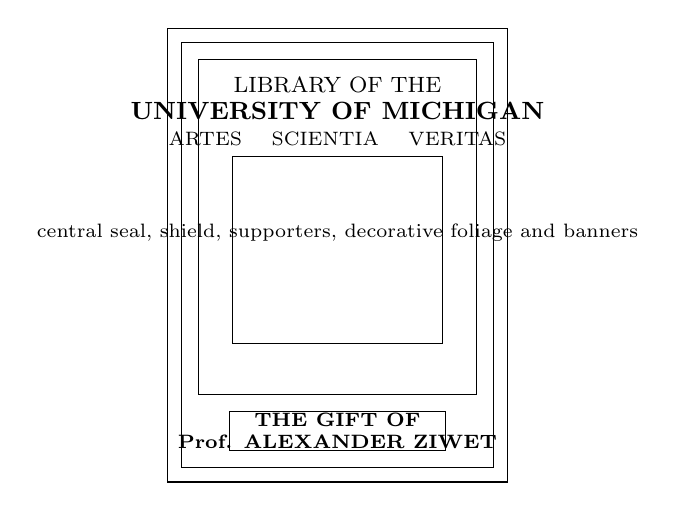
\begin{tikzpicture}[scale=.72]
  \draw[line width=.6pt] (0,0) rectangle (6,8);
  \draw (0.25,0.25) rectangle (5.75,7.75);
  \draw (0.55,1.55) rectangle (5.45,7.45);
  \node[align=center,font=\footnotesize] at (3,7.0) {LIBRARY OF THE};
  \node[align=center,font=\small\bfseries] at (3,6.55) {UNIVERSITY OF MICHIGAN};
  \node[align=center,font=\scriptsize] at (3,6.05) {ARTES \quad SCIENTIA \quad VERITAS};
  \draw (1.15,2.45) rectangle (4.85,5.75);
  \node[align=center,font=\scriptsize] at (3,4.4) {central seal, shield, supporters,\ decorative foliage and banners};
  \draw (1.1,.55) rectangle (4.9,1.25);
  \node[align=center,font=\scriptsize\bfseries] at (3,.9) {THE GIFT OF\\Prof. ALEXANDER ZIWET};
\end{tikzpicture}
\end{center}}
\newcommand{\hotu}{%
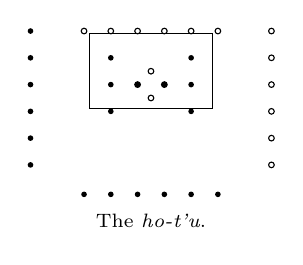
\begin{tikzpicture}[scale=.34,baseline=(current bounding box.center)]
\foreach \y in {0,1,2,3,4,5}{\fill (0,\y) circle (3pt);} % left vertical six
\foreach \x in {2,3,4,5,6,7}{\draw (\x,5) circle (3pt);} % top six open
\draw (2.2,2.1) rectangle (6.8,4.9);
\foreach \x/\y in {3/3,4/3,5/3,6/3,3/4,6/4,3/2,6/2}{\fill (\x,\y) circle (3pt);}
\foreach \x/\y in {4.5/3.5,4.5/2.5,4.0/3.0,5.0/3.0}{\draw (\x,\y) circle (3pt);}
\foreach \y in {0,1,2,3,4,5}{\draw (9,\y) circle (3pt);} % right vertical six
\foreach \x in {2,3,4,5,6,7}{\fill (\x,-1.1) circle (3pt);} % bottom six filled
\node[font=\scriptsize] at (4.5,-2.1) {The \emph{ho-t'u}.};
\end{tikzpicture}}
\newcommand{\loshudiagram}{%
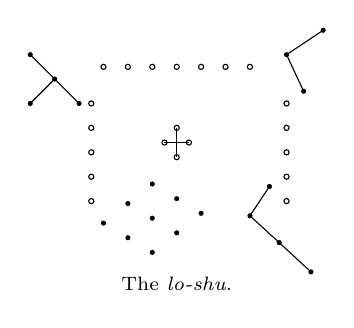
\begin{tikzpicture}[scale=.31,baseline=(current bounding box.center)]
\foreach \p in {(0,6),(1,5),(2,4),(0,4)}{\fill \p circle (3pt);} \draw (0,6)--(1,5)--(2,4); \draw (0,4)--(1,5);
\foreach \x in {3,4,5,6,7,8,9}{\draw (\x,5.5) circle (3pt);} 
\foreach \p in {(10.5,6),(12,7),(11.2,4.5)}{\fill \p circle (3pt);} \draw (10.5,6)--(12,7); \draw (10.5,6)--(11.2,4.5);
\foreach \y in {0,1,2,3,4}{\draw (2.5,\y) circle (3pt);} 
\foreach \p in {(5.5,2.4),(6.5,2.4),(6,1.8),(6,3)}{\draw \p circle (3pt);} \draw (5.5,2.4)--(6.5,2.4); \draw (6,1.8)--(6,3);
\foreach \y in {0,1,2,3,4}{\draw (10.5,\y) circle (3pt);} 
\foreach \p in {(3,-.9),(4,-.1),(5,.7),(4,-1.5),(5,-.7),(6,.1),(5,-2.1),(6,-1.3),(7,-.5)}{\fill \p circle (3pt);} 
\foreach \p in {(9,-.6),(10.2,-1.7),(11.5,-2.9),(9.8,.6)}{\fill \p circle (3pt);} \draw (9,-.6)--(10.2,-1.7)--(11.5,-2.9); \draw (9,-.6)--(9.8,.6);
\node[font=\scriptsize] at (6,-3.4) {The \emph{lo-shu}.};
\end{tikzpicture}}
\newcommand{\magicsquare}{\begin{array}{|c|c|c|}\hline 4&9&2\\\hline 3&5&7\\\hline 8&1&6\\\hline\end{array}}
\newcommand{\tocline}[2]{\noindent\parbox[t]{0.82\linewidth}{#1}\dotfill #2\par}
\newcommand{\toclinewide}[2]{\noindent\parbox[t]{0.86\linewidth}{#1}\dotfill #2\par}
\newcommand{\scandetail}[1]{{\footnotesize\emph{#1}}}
\newcommand{\teubnermark}{%

\begin{tikzpicture}[scale=.42,baseline=(current bounding box.center)]
  \draw[line width=.7pt] (-.55,-.55) rectangle (.55,.55);
  \node[font=\bfseries\Large] at (-.12,.08) {T};
  \node[font=\bfseries\Large] at (.17,-.10) {G};
\end{tikzpicture}}
\newcommand{\bookplateJobAA}{%
\begin{center}
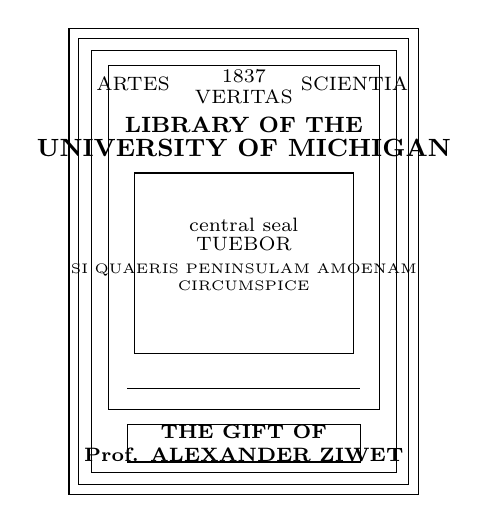
\begin{tikzpicture}[scale=.74]
  \draw[line width=.6pt] (0,0) rectangle (6,8);
  \draw[line width=.35pt] (0.17,0.17) rectangle (5.83,7.83);
  \draw[line width=.35pt] (0.38,0.38) rectangle (5.62,7.62);
  \draw[line width=.35pt] (0.68,1.47) rectangle (5.32,7.37);
  \node[font=\scriptsize] at (1.1,7.05) {ARTES};
  \node[font=\scriptsize] at (3.0,7.18) {1837};
  \node[font=\scriptsize] at (4.9,7.05) {SCIENTIA};
  \node[font=\scriptsize] at (3,6.83) {VERITAS};
  \node[align=center,font=\footnotesize\bfseries] at (3,6.35) {LIBRARY OF THE};
  \node[align=center,font=\small\bfseries] at (3,5.95) {UNIVERSITY OF MICHIGAN};
  \draw (1.12,2.42) rectangle (4.88,5.52);
  \node[align=center,font=\scriptsize] at (3,4.64) {central seal};
  \node[align=center,font=\scriptsize] at (3,4.30) {TUEBOR};
  \node[align=center,font=\tiny] at (3,3.86) {SI QUAERIS PENINSULAM AMOENAM};
  \node[align=center,font=\tiny] at (3,3.58) {CIRCUMSPICE};
  \draw[line width=.3pt] (1.0,1.82) -- (5.0,1.82);
  \draw (1.0,.56) rectangle (5.0,1.20);
  \node[align=center,font=\scriptsize\bfseries] at (3,.88) {THE GIFT OF\\Prof. ALEXANDER ZIWET};
\end{tikzpicture}
\end{center}}
\newcommand{\dotopen}[2]{\draw (#1,#2) circle (.095);}
\newcommand{\dotfilld}[2]{\fill (#1,#2) circle (.095);}
\newcommand{\hotuJobAA}{%
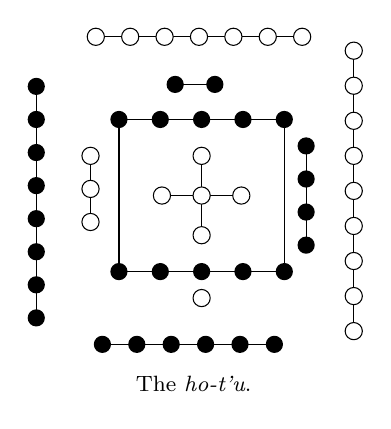
\begin{tikzpicture}[scale=.84,baseline=(current bounding box.center),line cap=round,line join=round]
  \draw[line width=.42pt] (0.00,0.65)--(0.00,4.15);
  \draw[line width=.42pt] (0.90,4.90)--(4.02,4.90);
  \draw[line width=.42pt] (1.00,0.25)--(3.60,0.25);
  \draw[line width=.42pt] (4.80,0.45)--(4.80,4.69);
  \draw[line width=.42pt] (.82,2.10)--(.82,3.10);
  \draw[line width=.42pt] (2.10,4.18)--(2.70,4.18);
  \draw[line width=.42pt] (1.25,1.35) rectangle (3.75,3.65);
  \draw[line width=.42pt] (4.08,1.75)--(4.08,3.25);
  \draw[line width=.42pt] (1.90,2.50)--(3.10,2.50);
  \draw[line width=.42pt] (2.50,1.90)--(2.50,3.10);
  \foreach \y in {0.65,1.15,1.65,2.15,2.65,3.15,3.65,4.15}{\mikafigfill{0.00}{\y}}
  \foreach \x in {1.00,1.52,2.04,2.56,3.08,3.60}{\mikafigfill{\x}{0.25}}
  \foreach \x in {1.25,1.875,2.50,3.125,3.75}{\mikafigfill{\x}{3.65}}
  \foreach \x in {1.25,1.875,2.50,3.125,3.75}{\mikafigfill{\x}{1.35}}
  \foreach \y in {1.75,2.25,2.75,3.25}{\mikafigfill{4.08}{\y}}
  \foreach \x in {2.10,2.70}{\mikafigfill{\x}{4.18}}
  \foreach \x in {0.90,1.42,1.94,2.46,2.98,3.50,4.02}{\mikafigopen{\x}{4.90}}
  \foreach \y in {0.45,0.98,1.51,2.04,2.57,3.10,3.63,4.16,4.69}{\mikafigopen{4.80}{\y}}
  \foreach \y in {2.10,2.60,3.10}{\mikafigopen{.82}{\y}}
  \foreach \x/\y in {1.90/2.50,2.50/2.50,3.10/2.50,2.50/1.90,2.50/3.10,2.50/.95}{\mikafigopen{\x}{\y}}
  \node[font=\footnotesize] at (2.38,-.35) {The \emph{ho-t'u}.};
\end{tikzpicture}}
\newcommand{\loshudiagramJobAA}{%
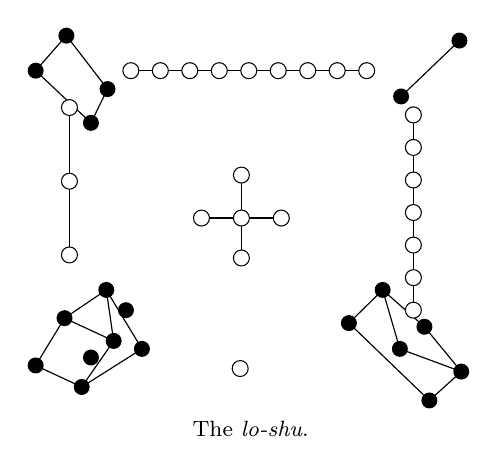
\begin{tikzpicture}[scale=.78,baseline=(current bounding box.center),line cap=round,line join=round]
  \draw[line width=.42pt] (.45,5.35)--(.95,5.92)--(1.62,5.05)--(1.35,4.50)--(.45,5.35);
  \draw[line width=.42pt] (2.00,5.35)--(5.84,5.35);
  \draw[line width=.42pt] (6.40,4.93)--(7.35,5.84);
  \draw[line width=.42pt] (1.00,2.35)--(1.00,4.75);
  \draw[line width=.42pt] (3.15,2.95)--(4.45,2.95);
  \draw[line width=.42pt] (3.80,2.30)--(3.80,3.65);
  \draw[line width=.42pt] (6.60,1.45)--(6.60,4.63);
  \draw[line width=.42pt] (.45,.55)--(1.20,.20)--(2.18,.82)--(1.60,1.78)--(.92,1.32)--(.45,.55);
  \draw[line width=.42pt] (.92,1.32)--(1.72,.95); \draw[line width=.42pt] (1.20,.20)--(1.72,.95)--(1.60,1.78);
  \draw[line width=.42pt] (5.55,1.24)--(6.10,1.78)--(6.78,1.18)--(7.38,.45)--(6.86,-.02)--(5.55,1.24);
  \draw[line width=.42pt] (6.10,1.78)--(6.38,.82)--(7.38,.45);
  \foreach \x/\y in {.45/5.35,.95/5.92,1.62/5.05,1.35/4.50}{\mikafigfill{\x}{\y}}
  \foreach \x/\y in {6.40/4.93,7.35/5.84}{\mikafigfill{\x}{\y}}
  \foreach \x/\y in {.45/.55,.92/1.32,1.20/.20,1.60/1.78,1.72/.95,2.18/.82,1.35/.68,1.92/1.45}{\mikafigfill{\x}{\y}}
  \foreach \x/\y in {5.55/1.24,6.10/1.78,6.38/.82,6.78/1.18,7.38/.45,6.86/-.02}{\mikafigfill{\x}{\y}}
  \foreach \x in {2.00,2.48,2.96,3.44,3.92,4.40,4.88,5.36,5.84}{\mikafigopen{\x}{5.35}}
  \foreach \y in {2.35,3.55,4.75}{\mikafigopen{1.00}{\y}}
  \foreach \x/\y in {3.15/2.95,3.80/2.95,4.45/2.95,3.80/2.30,3.80/3.65}{\mikafigopen{\x}{\y}}
  \foreach \y in {1.45,1.98,2.51,3.04,3.57,4.10,4.63}{\mikafigopen{6.60}{\y}}
  \mikafigopen{3.78}{.50}
  \node[font=\footnotesize] at (3.95,-.48) {The \emph{lo-shu}.};
\end{tikzpicture}}
\newcommand{\gridsquarebase}{\draw[step=1] (0,0) grid (7,7);}
\newcommand{\diagonsquare}{%
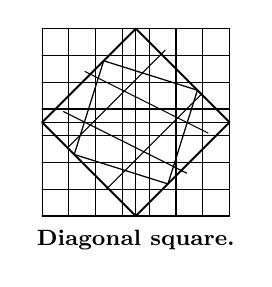
\begin{tikzpicture}[scale=.34,baseline=(current bounding box.center),line cap=round,line join=round]
  \gridsquarebase
  \draw[line width=.7pt] (3.5,7)--(7,3.5)--(3.5,0)--(0,3.5)--cycle;
  \draw[line width=.45pt] (2.3,5.8)--(5.8,4.7)--(4.7,1.2)--(1.2,2.3)--cycle;
  \draw (.8,3.9)--(5.4,1.6); \draw (1.6,5.4)--(6.2,3.1); \draw (1.0,2.6)--(4.6,6.2); \draw (2.4,1.0)--(6.0,4.6);
  \draw (3.5,0)--(3.5,7); \draw (0,3.5)--(7,3.5);
  \node[font=\footnotesize\bfseries] at (3.5,-.9) {Diagonal square.};
\end{tikzpicture}}
\newcommand{\breadthsquare}{%
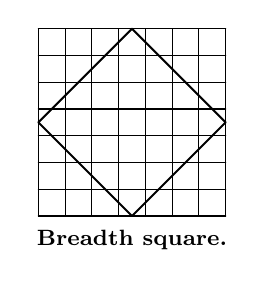
\begin{tikzpicture}[scale=.34,baseline=(current bounding box.center),line cap=round,line join=round]
  \gridsquarebase
  \draw[line width=.7pt] (3.5,7)--(7,3.5)--(3.5,0)--(0,3.5)--cycle;
  \draw[line width=.55pt] (3.5,7)--(7,3.5); \draw[line width=.55pt] (0,3.5)--(3.5,7);
  \node[font=\footnotesize\bfseries] at (3.5,-.9) {Breadth square.};
\end{tikzpicture}}
\newcommand{\lengthsquare}{%
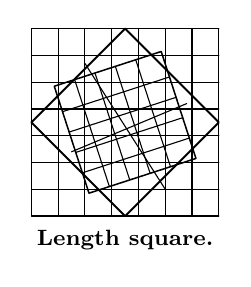
\begin{tikzpicture}[scale=.34,baseline=(current bounding box.center),line cap=round,line join=round]
  \gridsquarebase
  \draw[line width=.7pt] (3.5,7)--(7,3.5)--(3.5,0)--(0,3.5)--cycle;
  \begin{scope}[rotate around={18:(3.5,3.5)}]
    \draw[line width=.55pt] (1.4,1.4) rectangle (5.6,5.6);
    \foreach \x in {2.2,3.0,3.8,4.6}{\draw (\x,1.4)--(\x,5.6);} 
    \foreach \y in {2.2,3.0,3.8,4.6}{\draw (1.4,\y)--(5.6,\y);} 
  \end{scope}
  \draw (1.5,2.4)--(5.8,4.2); \draw (2.0,5.7)--(5.0,1.0);
  \node[font=\footnotesize\bfseries] at (3.5,-.9) {Length square.};
\end{tikzpicture}}
\newcommand{\fangtableA}{\begin{tabular}{|c|c|c|l|}\hline 1&2&3&1st class\\\hline 2&3&2&2nd ``\\\hline 3&1&1&3rd ``\\\hline 26&34&39&measures\\\hline\end{tabular}}
\newcommand{\fangtableB}{\begin{tabular}{|c|c|c|l|}\hline 1&0&3&1st class\\\hline 2&5&2&2nd ``\\\hline 3&1&1&3rd ``\\\hline 26&24&39&measures\\\hline\end{tabular}}
\newcommand{\fangtableC}{\begin{tabular}{|c|c|c|l|}\hline 0&0&3&1st class\\\hline 4&5&2&2nd ``\\\hline 8&1&1&3rd ``\\\hline 39&24&39&measures\\\hline\end{tabular}}
\newcommand{\fangtableD}{\begin{tabular}{|c|l|}\hline 36&third class\\\hline 99&measures\\\hline\end{tabular}}
\newcommand{\fangtableE}{\begin{tabular}{|c|c|c|l|}\hline 1&&2&1st class\\\hline &3&1&2nd ``\\\hline 4&1&&3rd ``\\\hline 1&1&1&measures\\\hline\end{tabular}}
\newcommand{\fangtableF}{\begin{tabular}{|c|c|c|l|}\hline $-5$&3&2&cows\\\hline 6&$-9$&5&sheep\\\hline 8&3&$-13$&hogs\\\hline $-600$&&1000&pieces\\\hline\end{tabular}}
\newcommand{\mikafigopen}[2]{\path[fill=white] (#1,#2) circle (.13);\draw[line width=.38pt] (#1,#2) circle (.13);}
\newcommand{\mikafigfill}[2]{\fill (#1,#2) circle (.13);}
\newcommand{\rodglyph}[2]{\raisebox{-0.25ex}{\includegraphics[height=#1,keepaspectratio]{#2}}}
\newcommand{\sourceasset}[2]{\begin{center}\includegraphics[width=#1,keepaspectratio]{#2}\end{center}}
\newcommand{\dec}[2]{#1{\cdot}#2}
\newcommand{\tg}{\mathop{\mathrm{tg}}}
\newcommand{\arcop}{\mathop{\mathrm{arc}}}
\newcommand{\versin}{\mathop{\mathrm{versin}}}
\newcommand{\rectsym}{\mathord{\raisebox{0.15ex}{\begingroup\setlength{\fboxsep}{0pt}\setlength{\fboxrule}{0.35pt}\fbox{\rule{0pt}{0.55ex}\rule{0.9ex}{0pt}}\endgroup}}}
\newcommand{\sourceassetJobAJ}[2][width=.84\linewidth]{\begin{center}\includegraphics[#1]{#2}\end{center}}
\newcommand{\dd}{\mathbin{\cdot}}
\newcommand{\congk}{\mathrel{\equiv}}
\begin{document}
\begin{titlepage}\centering
{\Large Yoshio Mikami}\par\vspace{1em}
{\Huge The Development of Mathematics\\[0.3em] in China and Japan}\par\vspace{1.5em}
{\large Leipzig: B.\ G.\ Teubner, 1913}\par
{\large Abhandlungen zur Geschichte der mathematischen Wissenschaften, XXX. Heft}\par\vfill
{\normalsize Complete transcription of the printed English text, page by page (366 PDF pages of the scan),\\
with the figures cropped from the scan. AI-transcribed; see the edition notes at the end.}\par
\end{titlepage}
\tableofcontents
% PDF page 1: cover, no printed text.
% PDF page 2: bookplate, no printed text.
% PDF page 3: call-number endpaper, no printed text.
% PDF page 4: blank endpaper, no printed text.
\scanpage{0005}{title page}
\begin{center}
ABHANDLUNGEN ZUR GESCHICHTE DER MATHEMATISCHEN\\
WISSENSCHAFTEN MIT EINSCHLUSS IHRER ANWENDUNGEN\\
BEGRÜNDET VON MORITZ CANTOR. XXX. HEFT.

\par\vspace{.35em}
\rule{\linewidth}{0.45pt}\\[-.35em]
\rule{\linewidth}{0.2pt}

\vspace{4em}
{\LARGE THE DEVELOPMENT\\ OF MATHEMATICS IN\\ CHINA AND JAPAN}

\vspace{2em}
BY

\vspace{1em}
{\large YOSHIO MIKAMI}\\[-.15em]
\rule{1.25em}{0.35pt}\\[-.42em]
\rule{.85em}{0.2pt}

\vspace{4em}
WITH 67 FIGURES IN THE TEXT

\vspace{3em}

\includegraphics[width=1.15cm]{pdf005-teubner-monogram.png}

\vspace{6em}
\begin{tabular}{ccc}
\underline{NEW YORK} & LEIPZIG: B. G. TEUBNER & \underline{LONDON}\\
G. E. STECHERT \& Co. & POSTSTRASSE 3 & WILLIAMS \& NORGATE\\
151--155 WEST 25th ST. & 1913 & 14 HENRIETTA STREET\\
& & COVENT GARDEN W. C.
\end{tabular}
\end{center}
\scanfooter

\scanpage{0006}{copyright page}
\begin{center}
\vfill
ALL RIGHTS RESERVED\\
PRINTED BY B. G. TEUBNER, DRESDEN
\end{center}
\scanfooter

\scanpage{0007}{dedication}
\begin{center}
THE AUTHOR DEDICATES\\[.5em]
THE PRESENT WORK TO HIS BENEFACTORS\\[1.2em]
{\large BARON D. KIKUCHI}\\[.5em]
Mr. N. OKAMOTO\\[.5em]
AND\\[.5em]
{\large Mr. T. ENDŌ}
\end{center}
\scanfooter

% PDF page 8: blank verso, no printed text.

\scanpage{0009}{Prefatory Note by George Bruce Halsted}
\begin{center}{\Large PREFATORY NOTE.}\end{center}

That English is already the world language, what proof could be more striking than its use in a history of Chinese mathematics written in Japan, revised in America, published in Europe? But naturally this is not the idiom of England nor of the United States, nor have I striven so to cramp it. My own slight connection with this work comes from Japan's being the first nation to appreciate the importance of the non-euclidean geometry, then available to them only in my Bolyai and Lobachevski, which led to the republication of both my little books in Tōkyō, each with an introductory Note by Baron Kikuchi, Imperial Minister of Education, now President of the University of Kyoto (the first dated Feb. 15, 1892). To realize how marvelously the dormant Japanese genius for geometry has since awakened, consult ``Mathematical Papers from the Far East'', edited by the Author of this history (Teubner, 1910), where 24 of the 55 papers (dating from 1892 to 1907) are in geometry.

It is a romantic piece of good fortune that our Author knew personally the last of the great mathematical giants of old Japan.

\begin{flushleft}Greeley, Colorado, U. S. A.\end{flushleft}
\begin{flushright}George Bruce Halsted.\end{flushright}
\scanfooter

\scanpage{0010}{Introductory Note, first page}
\begin{center}{\Large INTRODUCTORY NOTE.}\end{center}

Historical descriptions of the mathematics that has developed in China and Japan have been given by various authors. But these are all scattered in various journals, to which we have no easy access; we know of no single work that has been separately published, particularly devoted to the subject. There are, it is true, works like the Chinese Yüan Yüan's ``Biographies of Mathematicians and Astronomers'', that appeared at the close of the 18\textsuperscript{th} century, and T. Endo's ``History of Japanese Mathematics'', Tokyo, 1896. These are, indeed, valuable sources of information, but they are of little avail to European and American readers, being written in Chinese or Japanese. We have therefore undertaken the composition of the present volume. We shall be completely satisfied if we are able to give some knowledge of the subject to Occidental readers.

The results of my studies are by no means complete as a history. Therefore, I have avoided this title. My accounts are rather a collection of historical materials; even as such they are only too meagre and insufficient, and we must in advance inform our readers that there are still numerous other subjects considered by the old mathematicians of Japan and China, of which no mention is made in our book.

About the Japanese mathematics I am just collaborating a popularly written work with Dr. D. E. Smith, of New York. This history is only too simple, but it will give a good general view of the subject. Some parts of the productions of the Japanese mind considered in it are not reproduced in the present volume. We have therefore tried to give a general view and a chronology of the Japanese mathematics, which are followed by accounts of some particular subjects. This is the reason why I have adopted different plans of description for the Japanese mathematics and the Chinese science.

Throughout the whole volume I have instituted little or no comparison with the mathematical achievements of other nations. The course of development through which the mathematical ideas have arizen is also not specially accounted for, although studies in the line constitute my ideal. These are all left for further and maturer researches.

Old mathematical books, both written and printed, are now very difficult to collect. I have thus had considerable hardship in procuring
\scanfooter

\scanpage{0011}{Introductory Note, second page}
my materials. But despite all that, I must be exceedingly grateful for the kindness and sympathy shown by my friends, so that I have been able to carry on my studies chiefly on original sources of information, except for some parts, that are rather trifling. In completing this book I must acknowledge my indebtedness to the assistance rendered by these gentlemen. My thanks are especially due to Mr. T. Endō, Dr. Y. Fujikawa, the late T. Hagiwara, Prof. G. B. Halsted, Prof. T. Hayashi, Dr. K. Kano, Mr. C. Kawakita, Baron D. Kikuchi, Prof. S. Mikami, Mr. N. Okamoto, and Mr. K. Uyeno.

\begin{center}\rule{3cm}{0.4pt}\end{center}

The reading of Chinese ideograms has been done all in accordance with the way prevailing at present. In China the same ideograms or letters have been employed from old times down to our days, but their readings have gone through changes. The ideograms that are used in Japan are almost entirely those that have been brought from China, but the Japanese ways of reading are quite different from the Chinese ways, being, it is said, more like to one system followed of old in China. But the changes in the way of reading Chinese ideograms are in general being neglected by the Orientalists, so that we have followed their usage. Nor is it easy to trace the exact readings of various periods and of various localities. Even now the ideograms are not all read quite definitely; their readings are sometimes different in different parts of the country. Thus it is not seldom that the name of the same person is spelled in four or five different ways in the writings of the Orientalists of Europe and America. We must therefore ask our readers not to attach much importance to the spelling of Chinese names as given in the present work.

In the names of Chinese persons the family names are written first, being followed by the personal or individual names. In this respect the Chinese names differ from the Occidental names.

In Japan too the family names are written first, as in China.

In the Japanese language all syllables end in vowels with the single exception of those that end in \emph{n}. When the sound of \emph{n} comes before \emph{b}, or \emph{p}, or \emph{m}, this will be changed into \emph{m}, as is usually spelled by Japanese Occidentalists. For convenience sake we also employ spelling like \emph{kitto} or \emph{itchi}. The vowels \emph{a}, \emph{i}, \emph{u}, \emph{e}, \emph{o} should be pronounced something as in the German short sounds, their sounds being all very short. The long sounds of \emph{o} and \emph{u} will be denoted by \emph{ō} and \emph{ū}, which are of the same nature as the short sounds except for their lengths. \emph{Ai}, \emph{ei}, \emph{ii}, etc., should be read pronouncing the sounds of both vowels. \emph{Ku} should be pronounced almost like \emph{k}. Words properly spelled with \emph{ku} have sometimes been given only with the letter \emph{k}.

It is sometimes very difficult to know the correct reading of Japanese proper names. For instance the name of a mathematician
\scanfooter

\scanpage{0012}{Introductory Note, third page}
was read Yasushima by R. Fujisawa and Ajima by D. Kikuchi. But the family names are comparatively easy to read. The individual names are much more difficult. Thus we are accustomed to read such names in the general way of reading according to the sounds of the ideograms themselves irrespective of the true way of reading. We read Seki Kōwa, although his personal name Kōwa should have been read Takakazu. Takahashi Shiji's individual name was read Shigetoki or Yoshitoki by T. Hayashi, but others read it Munetoki. But in actuality we know nothing of the true reading of his name, and so we have to read it only Shiji according to the general reading of the ideograms. The differences of readings between me and Hayashi (in his \emph{Brief History of Japanese Mathematics}, in the \emph{Nieuw Archief voor Wiskunde}) have arisen mostly in this way.

A descendant of the astronomer Yamaji Shūjū is an eminent historian and thinker, but he does not know, as he has personally told me, how the name Shūjū should have been read. Saitō Gigi was T. Hagiwara's master, but the latter told me that he had never learned of the true reading of his master's individual name Gigi. The individual names of the old Japanese were used upon grave or serious occasions only, such as in signing books, for instance. On common occasions, these names were never employed, every one bearing his familiar name. That of Seki was Shinsuke, and thus he is sometimes called Seki Shinsuke.

The old Japanese manuscripts are never free from various errors; it is even so with the hand-writings of the authors. In the transcripts which have gone through the hands of several copyists, the errors are especially numerous. Those which we have utilised in reference are not free from these faults. When we compare various copies of the same manuscripts we sometimes find some parts of these quite differing from one another. But the errors committed in these manuscripts are not generally easy to be found, and so in my accounts of them the errors are not necessarily all corrected. However, we hope, the readers who take these circumstances into account will not blame us too much for such faults as are left unnoticed in our work.

\begin{flushleft}Ōhara in Kazusa, September 20\textsuperscript{th}, 1910.\end{flushleft}
\begin{flushright}Y. Mikami.\end{flushright}
\scanfooter


\scanpage{0013}{Contents, first page}
\begin{center}{\Large CONTENTS.}\end{center}
\begin{flushright}{\footnotesize Page}\end{flushright}
\begingroup\small\setlength{\parskip}{0.18em}
\tocline{Prefatory note. By Prof. G. B. Halsted}{V}
\tocline{Introductory note}{VI}
\tocline{Contents}{IX}
\tocline{Part I. The Chinese Mathematics}{1}
\tocline{\quad Chap. 1. Earliest period of Chinese mathematics}{1}
\tocline{\quad Chap. 2. The Chou-Pei}{4}
\tocline{\quad Chap. 3. The Chiu-chang Suan-shu}{8}
\tocline{\quad Chap. 4. The Sun-Tsŭ Suan-ching or the arithmetical classic\\\hspace*{2.8em}of Sun-Tsŭ}{25}
\tocline{\quad Chap. 5. The Hai-tao Suan-ching or the Sea-Island Arithmeti-\\\hspace*{2.8em}cal Classic}{33}
\tocline{\quad Chap. 6. The Wu-t'sao Suan-ching and the works of Hsia-hou\\\hspace*{2.8em}Yang, Chang Ch'iu-chien and Chen Luan}{37}
\tocline{\quad Chap. 7. The circle-measurements by older Chinese mathematicians}{46}
\tocline{\quad Chap. 8. Wang Hsiao-t'ung and cubic equations}{53}
\tocline{\quad Chap. 9. On the Indian influence}{56}
\tocline{\quad Chap. 10. Ch'ên Huo}{61}
\tocline{\quad Chap. 11. Ch'in Chiu-shao}{63}
\tocline{\quad Chap. 12. Li Yeh}{79}
\tocline{\quad Chap. 13. Yang Hui}{84}
\tocline{\quad Chap. 14. Chu Shih-chieh}{89}
\tocline{\quad Chap. 15. The Arabian influence, and Kuo Shou-ching}{98}
\tocline{\quad Chap. 16. The mathematics of the Ming Dynasty}{108}
\tocline{\quad Chap. 17. The introduction of the European mathematics}{112}
\tocline{\quad Chap. 18. The revival of old modes of mathematics and the state\\\hspace*{2.8em}of subsequent years}{120}
\tocline{\quad Chap. 19. Later progress of the solution of equations}{128}
\tocline{\quad Chap. 20. The studies about the values of $\pi$ by later Chinese\\\hspace*{2.8em}mathematicians}{135}
\tocline{\quad Chap. 21. Analytical studies about circle-measurement. Infinite series}{142}
\tocline{Part II. The Japanese Mathematics}{156}
\tocline{\quad Chap. 22. A general view of the Japanese mathematics}{156}
\tocline{\quad Chap. 23. A chronology of the Japanese mathematics}{178}
\tocline{\quad Chap. 24. Seki's conception of the determinant}{191}
\tocline{\quad Chap. 25. The values of $\pi$ used by the Japanese mathematicians}{200}
\tocline{\quad Chap. 26. Japanese mathematicians' studies of the spherical volume}{203}
\tocline{\quad Chap. 27. Japanese mathematicians' studies of finding the surface\\\hspace*{2.8em}of a sphere}{206}
\endgroup
\scanfooter

\scanpage{0014}{Contents, second page}
\begin{flushright}{\footnotesize Page}\end{flushright}
\begingroup\small\setlength{\parskip}{0.18em}
\tocline{\quad Chap. 28. A formula for the square of an arc of a circle in the\\\hspace*{2.8em}Kwatsuyō Sampō of 1709}{210}
\tocline{\quad Chap. 29. Some series for $\pi$ used by the Japanese mathematicians}{213}
\tocline{\quad Chap. 30. Kurushima's circle-measurement}{217}
\tocline{\quad Chap. 31. Kurushima's method of continued fractions for the\\\hspace*{2.8em}quadratic surd}{223}
\tocline{\quad Chap. 32. Problems in indeterminate analysis in Matsunaga's manu-\\\hspace*{2.8em}script}{229}
\tocline{\quad Chap. 33. The indeterminate equation $x^p - ky = a$}{237}
\tocline{\quad Chap. 34. Ajima's Renjutsu Henkan}{238}
\tocline{\quad Chap. 35. Ajima's study of circles successively inscribed forming a\\\hspace*{2.8em}crown within a circle}{243}
\tocline{\quad Chap. 36 Aida's solution of the indeterminate equation $x_1^2+x_2^2$\\\hspace*{2.8em}$+x_3^2+x_4^2+x_5^2=y^2$}{247}
\tocline{\quad Chap. 37. Aida's studies of the ellipse}{249}
\tocline{\quad Chap. 38. Shiraishi's calculation of the ellipsoidal surface}{256}
\tocline{\quad Chap. 39. Sakabe-Kawai's solution of equations}{260}
\tocline{\quad Chap. 40. Some tables used in the y\,e\,n\,r\,i calculations, and the\\\hspace*{2.8em}equation of infinite degree}{268}
\tocline{\quad Chap. 41. On the wedge-sections in Hasegawa's Kyūseki Tsūkō}{284}
\tocline{\quad Chap. 42. Magic squares}{290}
\tocline{\quad Chap. 43. The catenary}{294}
\tocline{\quad Chap. 44. Hagiwara Teisuke}{301}
\tocline{\quad Chap. 45. Hagiwara's formula for the area of the curve described\\\hspace*{2.8em}by a sphere rolling round an anchor-ring standing on a plane}{311}
\tocline{\quad Chap. 46. The skew surface}{315}
\tocline{\quad Chap 47. A short notice of the historical studies of the Japanese\\\hspace*{2.8em}mathematics}{322}
\tocline{Index}{331}
\endgroup
\scanfooter

\scanpage{0015}{Part I, Chapter 1, first page}
\begin{center}
PART I.\\[1em]
{\Large THE CHINESE MATHEMATICS.}\\[1em]
CHAPTER 1.\\
{\large EARLIEST PERIOD OF CHINESE MATHEMATICS.}
\end{center}
\phantomsection\addcontentsline{toc}{section}{Part I. The Chinese Mathematics}
\phantomsection\addcontentsline{toc}{subsection}{Chapter 1. Earliest Period of Chinese Mathematics}

China is one of oldest nations in the world. In ancientness China can be compared only with Egypt and Babylon, but with no other countries. However far we go back on our search into remoter periods in Chinese history, we still find there some traces of early culture. According to the native annals, the Chinese have enjoyed their civilization for tens of milleniums in the past. With their early rise of a civilised life, mathematics dawned too undoubtedly in an early age. The Chinese have, from the oldest times, been a race most observant of religious rites and taking utmost care in calendrical regulations; and consequently there can be no doubt at all as to the careful culture of arithmetical arts even in ancient days. But we are utterly at a loss when we try to investigate the growth of the science in remote antiquity, for old documents or records are entirely wanting.

There is no doubt as to China being an ancient nation. But the Chinese did not always inhabit the vast land watered by the Yellow River and the Yangtse Chiang; they came from the West to settle where they now live. They are sometimes referred to as a race a-kin to the Babylonians. As some scholars point out, the civilizations of the two peoples in great antiquity resemble each other in a considerable measure. When so, is it not possible that the Chinese had in ancient times a knowledge in arithmetical rules the same as possessed by their brethren in the west? We are however at present unable either to affirm or deny this view. We are not therefore going, at least in this place, to argue about the interrelations of the mathematics developed in China and cultivated by the Babylonians. So this

\scanfooter

\scanpage{0016}{Part I, Chapter 1, second page}
\setcounter{footnote}{0}
interesting question must be left untouched for the results for further studies.

According to old documents, Huang-Ti or the Yellow Emperor made I-hai divine the sun, Chang-i divine the moon, Yü-ch’ü divine the stars, Ling-lun establish the musical notes, Tai-nao construct the \emph{chia-tsŭ} or sexagesimal system, Li-shou invent the numbers or the art of numbers, and Yung-ch’éng employ all these six arts to regulate calendars.\footnote{Yüan Yüan, the \emph{Ch’ou-jen Ch’uan} or ``Biographical Collections of Astronomers and Mathematicians'', Book 1.} As is well known the Yellow Emperor reigned over China in the 27\textsuperscript{th} century B. C.

The \emph{chia-tsŭ} that has been ever employed from the time of the Yellow Emperor down to the present day, consists in coordinating the two systems, which are \emph{chia}, \emph{i}, \emph{ping}, \emph{hsü}, \emph{chi}, \emph{kong}, \emph{hsin}, \emph{jen}, \emph{kuei}, and \emph{tsŭ}, \emph{ch’ou}, \emph{yin}, \emph{mao}, \emph{ch’én}, \emph{szŭ}, \emph{wu}, \emph{wei}, \emph{shen}, \emph{yu}, \emph{wu}, \emph{hai}.

In the \emph{chia-tsŭ} system of enumeration, the first, second, and so forth, are represented as \emph{chia-tsŭ}, \emph{i-ch’ou}, \ldots\ Or if we represent the members of the two cycles of 10 and 12 for the sake of plainness by $A_1,A_2,\ldots,A_{10}$ and $B_1,B_2,\ldots,B_{12}$, respectively, then the enumeration will follow as indicated below:
\[
\begin{aligned}
A_1B_1&=1,\quad A_2B_2=2,\ldots, A_{10}B_{10}=10,\\
A_1B_{11}&=11,\quad A_2B_{12}=12,\quad A_3B_1=13,\ldots, A_{10}B_8=20,\\
A_1B_9&=21,\ldots, A_4B_{12}=24,\quad A_5B_1=25,\quad A_6B_2=26,\\[-.5em]
&\hspace{4em}\cdots\cdots\cdots\cdots\cdots\\[-.5em]
A_{10}B_2&=50,\quad A_1B_3=51,\ldots, A_9B_{11}=59,\quad A_{10}B_{12}=60.
\end{aligned}
\]
Above 60 the same enumeration returns again in repeated cycles. The years and the days have been numbered in this way. Directions were also indicated by this way of dividing the whole circumference into 60 parts.

Li-shou is sometimes referred to as the author of an arithmetical work entitled the \emph{Chiu-chang} or ``Nine Sections'', from which the still extant \emph{Chiu-chang Suan-shu} or ``Arithmetic in Nine Sections'' has arisen by successive revisions. This opinion is probably no more than a fiction. There was indeed a work with the title of the \emph{Huang-Ti Chiu-chang} or the \emph{Yellow Emperor's Nine Sections} some time at the end of the \emph{Sung Dynasty}, which, however, appears to be a mere invention of later scholars. We have no means of knowing of what kind of arithmetic was the arts Li-shou established at so early a date
\scanfooter

\scanpage{0017}{Part I, Chapter 1, third page}
\setcounter{footnote}{0}
as over 3500 years ago. We may only reasonably guess the science developed in so great an antiquity must necessarily have been of a mere rudimental kind. So highly developed a system as laid down in the ``Arithmetic in Nine Sections'' could not exist in the times of Huang-Ti, we believe. As to the contents of the treatise just mentioned we shall try to give a description in a special chapter devoted to it.

In the sacred book of \emph{I-ching}, the chapter on \emph{Hsi-tzŭ}, it is stated that a river made the \emph{t’u} and the Lo made the \emph{shu}. This means the figures called the \emph{ho-t’u} and the \emph{lo-shu} were employed in fortune-telling. According to tradition the former came down from the time of the Emperor Fu-hi in the 29\textsuperscript{th} century B. C., when a dragon-horse had discovered himself at a river and his footsteps had left the figures of the \emph{pa-kua}, which have served in sooth-saying. The \emph{lo-shu} comes down to us from the time of the sage Yü, who was a great statesman and enlightened emperor. When he was embanking upon the calamitous ever-flowing Yellow River, there appeared a divine tortoise, whose back was decorated with a figure made up of the numbers from 1 to 9. The great sage recorded and applied it. The \emph{ho-t’u} and the \emph{lo-shu} occur in Chinese works as shown below.

\begin{center}
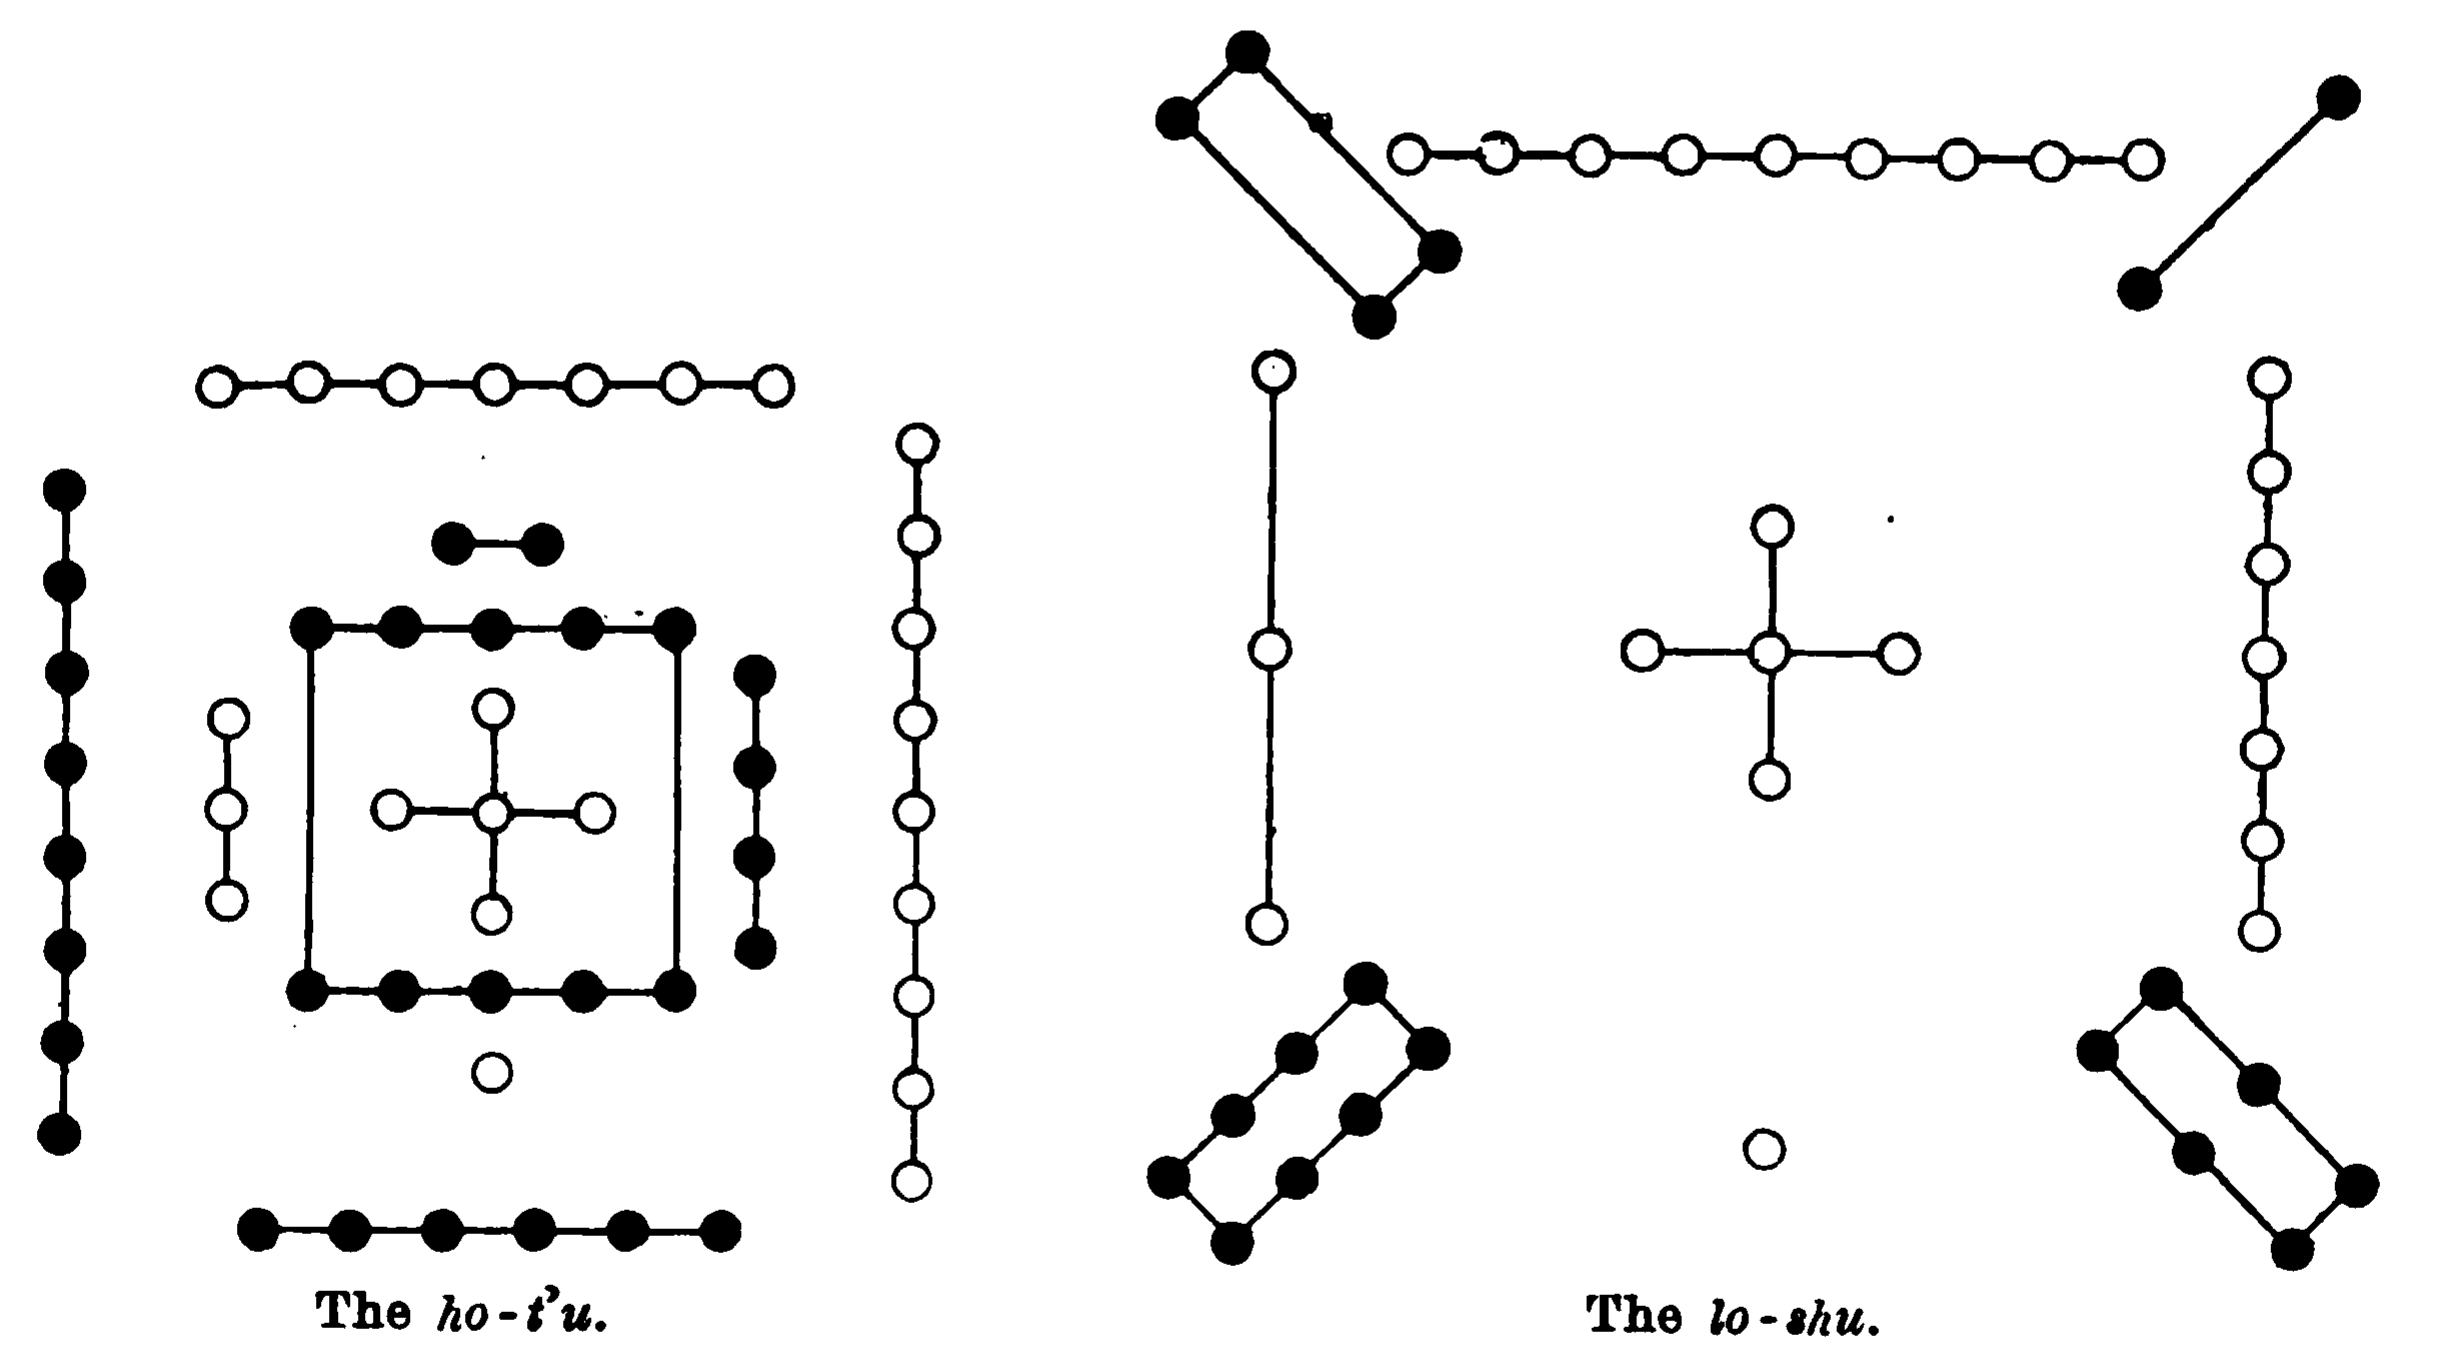
\includegraphics[width=.92\linewidth]{pdf017-hotu-loshu.png}
\end{center}

The \emph{lo-shu} is a magic square with the nine figures as its elements as annexed. It comes therefore that the magic squares were called by that name in later China and also by some earlier Japanese mathematicians.\footnote{The Chinese \emph{lo-shu} was read \emph{rakusho} in Japan.}
\begin{center}
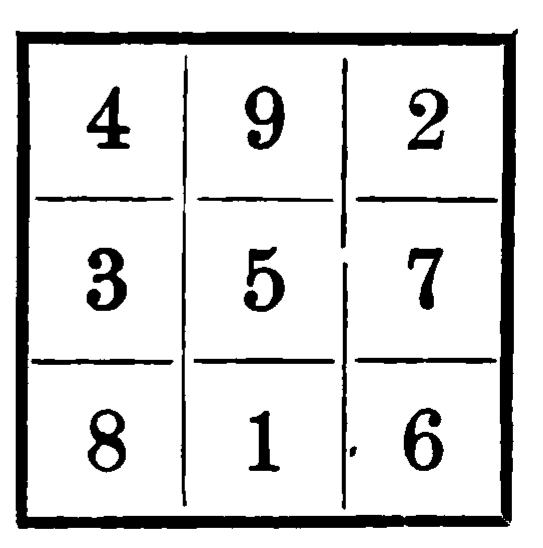
\includegraphics[width=.20\linewidth]{pdf017-magic-square.png}
\end{center}
\scanfooter

\scanpage{0018}{Part I, Chapter 2, printed page 4}
\begin{center}
CHAPTER 2.\quad THE CHOU-PEI.
\end{center}
\phantomsection\addcontentsline{toc}{subsection}{Chapter 2. The Chou-Pei}

The oldest mathematical work left by the ancient Chinese that remains extant to this very day is doubtless the \emph{Chou-pei} or the \emph{Chou-pei Suan-ching}. The word \emph{suan-ching} should be literally rendered by ``a mathematical classic'' or ``a sacred book of arithmetic''. But in strictness, the \emph{Chou-pei} is no mathematical work, it is one in which calendrical subjects are considered. Yet it is of unsurmountable interest in the history of the Chinese mathematics.

The author of the \emph{Chou-pei} has ever remained unknown; nor is known the date when it was composed. It is also questionable whether the whole of the book was composed at a single time or at several different times. The \emph{Chou-pei} as it has been handed down to us consists of two books, of which the second treats of calendrical theories that little concern us in this place. In the first book of the \emph{Chou-pei} there is laid down a famous dialogue that had taken place between the sage prince Chou-Kong and his learned minister Shang Kao. The dialogue is followed by another between Ying Fang and Ch'ên-Tsŭ. It is not known in what age these lived. As is generally believed, or rather imagined, this second dialogue seems to be an addition supplied by a subsequent writer. Next to the second dialogue there is still another passage written by or recorded as taught by Lü-Shih, that is, by Lü Pu-i, who was a powerful minister of the Monarchy of Ch'in in the 3rd century B. C. In any case, therefore, the personages represented in the second dialogue must have lived at the end of the Chou Dynasty or previous to that time.

The \emph{Chou-pei} has been preserved through the commentaries of Chang Chun-ch'ing, Ch'ên Luan, Li Ch'un-fêng and others. The date of the first of these commentators is given by later native writers as unknowable. But his preface refers to an astronomical work, the \emph{Ling-hsien}, that was composed by Chang Hêng. This proves well that Chang Chun-ch'ing lived in or subsequent to the 2\textsuperscript{nd} century A. D., for Chang Hêng died in 139 A. D.

Although the composition of the \emph{Chou-pei} or at least of its augmented parts may be of a comparatively recent date, yet the dialogue recorded in it serves to reveal to us the state of mathematical studies the Chinese had attained in so early an age as the 12\textsuperscript{th} century B. C., for it was in the year 1105 that Chou-Kong died. Chou-Kong was a brother to Wu-Wang, King of the Chou Dynasty, and
\scanfooter

\scanpage{0019}{Chapter 2, printed page 5}
ruled over China as a regent when his youthful nephew Ch'êng-Wang sat on the throne.

The dialogue runs as follows:

``Of old, Chou-Kong inquired of Shang Kao: As I have heard that you are versed in the arts of numbers, so let me ask you. In old times Fu-hi measured the heavens and regulated the calendar. But are neither the heavens susceptible of climbing, nor is the earth of measurement by means of our measures. Whence will it be, then, that their numbers are deduced from?

``Shang Kao replied: The art of numbers is derived from the circle and the square. The circle is derived from the square, and the square from the \emph{kuei} or the right-angled lineal. The lineal comes from 9 into 9, which makes 81. Thus break the lineal, and make the \emph{kou} or breadth 3, the \emph{ku} or length 4; then the distance joining the corners is 5. Take the squares of the outer numbers, and halving, the lineal is obtained.''

This last sentence is very hard to be appropriately understood, as it is originally given in the text of the \emph{Chou-pei}, as well as in Chang's comment. It perhaps means that, taking the sum of the squares on two sides of a right triangle and extracting its square root, the hypotenuse will be obtained.

Shang Kao continues:

``Surrounding (a space), set them on the board, when we get 3, 4 and 5, for the two sets are both 25, which we call \emph{chi-chü} or the laying of \emph{chüs}. The means, therefore, which Yü had used in governing the world arise from these numbers.''

Here the following three diagrams are intervened.

\begin{center}
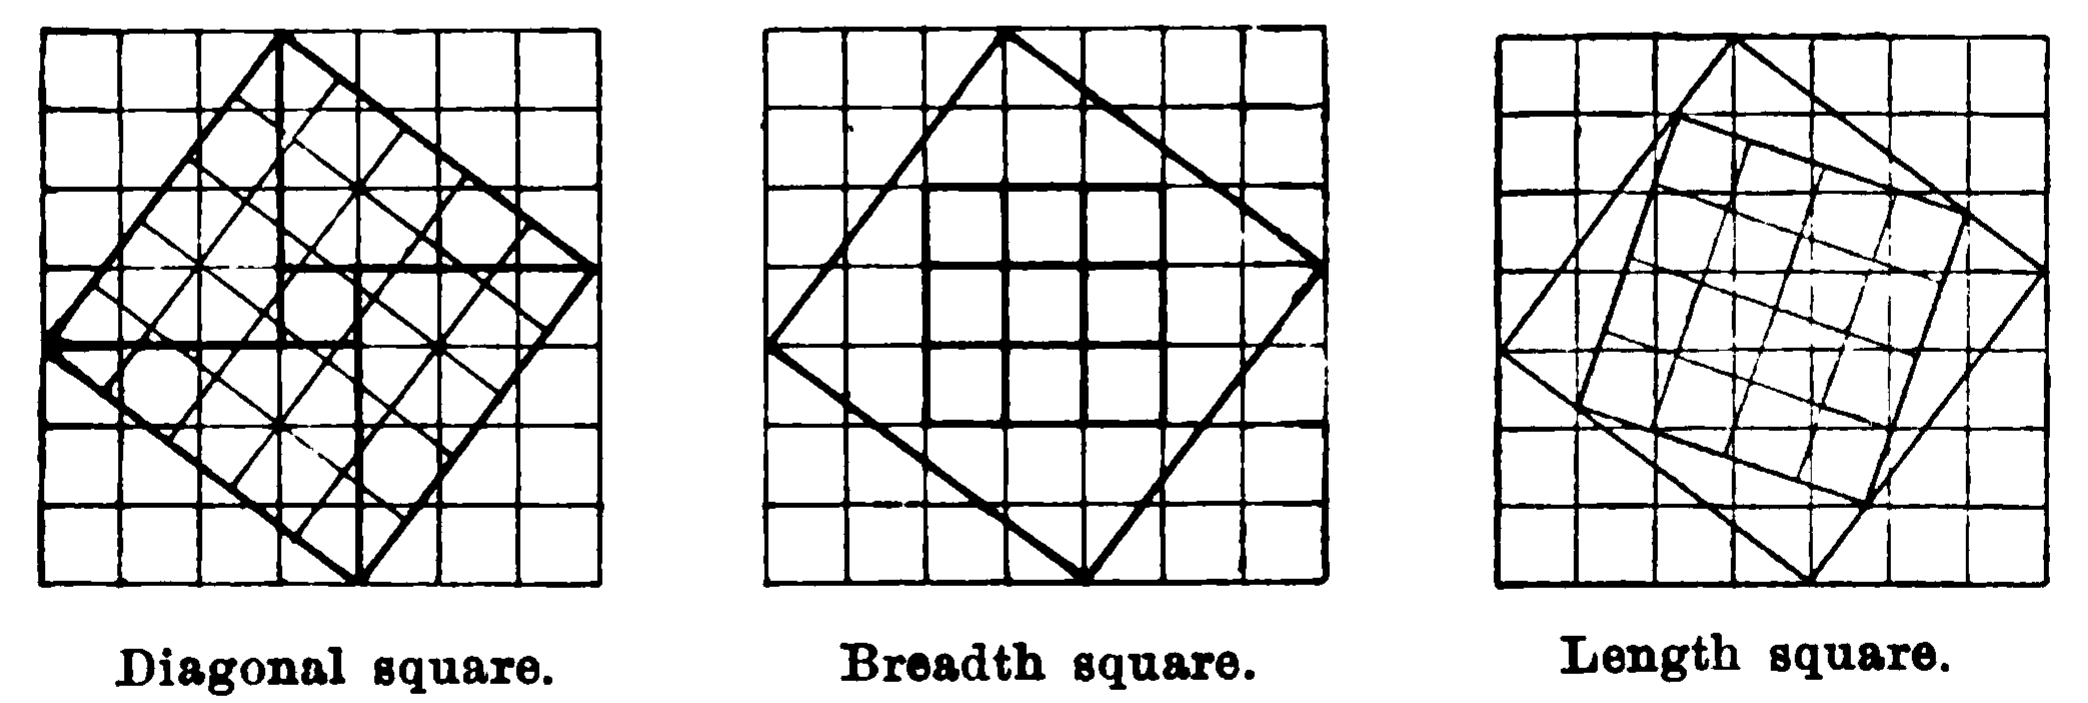
\includegraphics[width=.85\linewidth]{pdf019-chou-pei-three-diagrams.png}
\end{center}

``Chou-Kong said: Ah mighty is the art of numbers! I dare ask you of the employment of the \emph{chüs} or lineals.

``Shang Kao replied: The horizontal lineal adjusts the lines; the vertical lineal looks on the height; the overturned lineal measures the depth; the lying lineal serves to know distance; the turning lineal makes the circle; and double lineals make a square. The square be-
\scanfooter

\scanpage{0020}{Chapter 2, printed page 6}
\setcounter{footnote}{0}
longs to the earth, the circle to the heaven; heaven is round and earth is square.''

In this place Chang Chun-ch'ing's note most interests us, for he runs:`` Things are round or pointed; numbers are odd or even. The heaven moving describes a circle, whose subordinate numbers are odd. The earth resting makes a square, whose subordinate numbers are even. These are said concerning the doctrine of the \emph{yin-yang} or the positiveness and negativeness\footnote{The \emph{yin} and \emph{yang} are the basic principles of the dualistic philosophy of the \emph{I-ching}, one of the sacred books of China. The word \emph{yang} means positivity, sun-shine, male, increase, etc., and \emph{yin} negativity, shadow, female, decrease, and so forth.}, and do not represent the actual forms of the heavens and the earth. The heaven cannot be perceived through to its limits; the earth cannot be followed to its ends. How then could they be affirmed to be round or squared?''

This note is perfectly in accordance with the view entertained by a Christian missionary who long stayed in China, a view which Moritz Cantor adopts in his work as interestingly probable.\footnote{M. Cantor, \emph{Vorl. üb. Geschichte der Mathematik}, I., dritte Auflage, 1907, p. 680.} According to the missionary, heaven and earth were symbolic for 3 and 4; and besides the number 3 belongs to the circle, whose circumference is three times its diameter; 4 belongs naturally to the square; and therefore follows the further comparisons of the heaven with the circle and the earth with the square.

In the sacred book, \emph{I-ching}, it is stated: Heaven one and earth two; heaven three and earth four; heaven five and earth six; and so on. This and allied passages in the works of various philosophers and astrologers of different ages seem to make certain the correctness of the entertained view.

Shang Kao proceeds:

``The number pertaining to the square serves the standard, and the circle is derived from the square.''

Here Chang Chun-ch'ing makes his comment that this passage is intended to mean the measurement of the circular area as that of a square by multiplying together its semi-circumference and radius.

Shang Kao goes on:

``Umbrella-formed is the heaven. The heaven is bluish black; the earth yellowish red. The number (or rather the form) pertaining
\scanfooter

\scanpage{0021}{Chapter 2, printed page 7}
\setcounter{footnote}{0}
to the heaven is formed, when bluish black is its front, reddish yellow its back. And one moulds the situations of the heaven and earth.

``Therefore one who knows of the earth is intelligent, one who knows of the heaven is sage.\footnote{Here it is meant that no one can deal with astronomical subjects unless he be a distinguished wise man.} The knowledge comes from the shadow, and the shadow comes from the gnomon or the lineal. The lineal together with the number rules and guides everything in the universe as is desired.

``Chou-Kong said: Excellently good.''

As will appear from the text in the dialogue, the Chinese in the time of Chou-Kong had known of the Pythagorean theorem, so important in application, that relates to the squares described upon the sides of a right-angled triangle. Although it is not enunciated in such a concise geometrical form as is given in Euclid, yet there is no denying the fact of its being soundly established by the Chinese in great antiquity.

The Chinese are sometimes considered as a race akin in blood to the ancient Babylonians. The latter seem to have been in possession of the same relation at least for the special case of the sides 3, 4 and 5. If the Chinese could be supposed to have borrowed their knowledge from their Babylonian kinsmen, then why could the latter not be thought on the contrary to have learned from the former? Pythagoras who flourished six long centuries later than Chou-Kong, is he not said to have traveled in the east to Babylon and perhaps farther on probably to India? Will it not be probable that he had seen the theorem that was destined to be connected with his name on his travel? Might he not have encountered it brought from China in some unknown way? The lapse of time between him and Chou-Kong justly makes the matter an open question.

In the second dialogue of the \emph{Chou-pei}, the learned Ch'ên-Tsŭ instructs Ying Fang in more material or well-organised topics than Shang Kao does in the first dialogue to Chou-Kong. But the whole concerns solely to calendrical or astronomical theories, and it is of a comparatively later date, and so we shall not dare give it in full. Only a stage of Ch'ên-Tsŭ's statement will be reproduced:

``The sun lies at the summer solstice 16000 Chinese miles to the south, and at the winter solstice 135000 miles to the south, where
\scanfooter

\scanpage{0022}{Chapter 2 ending and Chapter 3 opening, printed page 8}
\setcounter{footnote}{0}
vertical rods throw no shadow at the midday.\footnote{These distances are inferred in a peculiar manner as is given in the book from the lengths of shadows of the gnomon, the earth being supposed to be flat.} Therefore the positions of the sun at the two solstices are 119000 miles distant from each other, and at midnight the sun lies the same way distant to the north. Hence the length of 238000 miles represents the diameter of the sun's orbit at the summer solstice, when its length of revolution measures 714000 miles''

As Ch'ên-Tsŭ states further:

``At the winter solstice the sun's orbit has a diameter of 476000 miles, the circumference of the orbit being 1428000 miles.''

In these cases the circumference of the circle is taken as three times its diameter, as will be easily seen. The Chinese had used the value of $\pi=3$ from old times.

In Lü's argument found in the \emph{Chou-pei} is stated that one year consists of $365\frac14$ days, and that the circumference of a circle is divided into $365\frac14$ degrees. Such a usage is commonly believed to have arisen in a far earlier period than the age in which Lü lived.

In the second book of the \emph{Chou-pei} we read a passage to the effect that arranging the diameter $121\cdot 75$ feet and multiplying it by 3, one should get $365\frac14$ feet, which corresponds to the $365\frac14$ degrees in the circumference of the heavens.

Among Lüh-Shih's considerations there is given a case of division by a fraction. To divide 119000 miles by $182\frac58$ days, both the dividend and the divisor are first multiplied by the denominator of the divisor, which is 8 in the present case; or the division is carried out after both the members are rendered to assume integral values by changing the unit. Though the description is given in a language somewhat obscure, it seems to convey no other meaning than we have mentioned.

\begin{center}
CHAPTER 3.\\
THE CHIU-CHANG SUAN-SHU.
\end{center}
\phantomsection\addcontentsline{toc}{subsection}{Chapter 3. The Chiu-Chang Suan-Shu}

The Chinese mathematical treatise now extant next in age to the \emph{Chou-pei} is doubtless the \emph{Chiu-chang Suan-shu} or the ``Arithmetic in Nine Sections''. The \emph{Chou-pei} is no work on arithmetic when properly spoken of, while the \emph{Chiu-chang} is a true arithmetical treatise,
\scanfooter

\scanpage{0023}{Chapter 3, printed page 9}
\setcounter{footnote}{0}
the oldest therefore that remains to the present day. This is besides the most extensive and far-reaching of all treatises that concern mathematics belonging to older times in China. The \emph{Chiu-chang} has therefore an invaluable interest in history.

Neither the author of the ``Arithmetic in Nine Sections'' nor the date of its composition is exactly known to us. But so far as we can learn from what the commentator Liu Hui, who lived in the third century of the Christian era, records in the preface of his edition, the work was a remnant of old writings, which was revised or enlarged by Chang T'sang and Ching Ch'ou-ch'ang in the first part of the Han Dynasty.\footnote{The Han Dynasty begins with the accession of the Emperor Kao-tsu to the throne in 202 B. C. The Dynasty flourished for two centuries, until it was upset by the usurpation of Wang Mang at the beginning of the 1st Christian century.} As is popularly known, all books were burned and all scholars were buried in the year 213 B. C., by an edict of the mighty and despotic emperor Shih Hoang-ti of the Ch'in Dynasty, without saving the harmless treatises of arithmetic or of astronomy. It comes therefore that there remains no book on arithmetic that belongs to a remoter age. But Shih Hoang-ti's empire fell to pieces soon after his death\footnote{Shih Hoang-ti died in 210 B. C.}, and in the beginning of the succeeding dynasty, the Han, the lost books were searched after and learning was seen soon reviving. It was just at this juncture that Chang T'sang made his appearance. According to Liu Hui, the commentator, Chang had found some old writings, upon which he based the composition of his ever-valued \emph{Chiu-chang Suan-shu}. The work was revised for a second time later on by Ching Ch'ou-ch'ang. The original treatise Chang had used in composing his work is generally believed to have been the \emph{Chiu-chang}, that was edited by Chou-Kong's orders, a fact that is however little trustworthy. It is not known whether there had been such a work of Chou-Kong's at all. As we read in the calendrical department of the \emph{Chin-Shu}\footnote{The same is also recorded in the \emph{Sui-Shu} or ``Records of the Sui Dynasty''.} or the ``Records of the Chin Dynasty'', Liu Hui's commentary on the ``Arithmetic in Nine Sections'' was written in 263 A. D., in the reign of Ch'ên-liu-Wang, King of the Wei Monarchy. Commentaries on the same book were again written by Li Ch'un-fêng in the 7\textsuperscript{th} century.

Biographical notices of Chang T'sang are given in Szü-ma Ch'ien's \emph{Shih-chi} or ``Historical Records'' and Pan Ku's \emph{Han Shu} or ``Records
\scanfooter

\scanpage{0024}{Chapter 3, printed page 10}
\setcounter{footnote}{0}
of the Han Dynasty''. According to these records, which are almost identical, Chang was a civil servant of the Ch'in government in his early life. Afterwards he fought under the first of the Han emperors, when he achieved many brilliant exploits. After the order of things had been restored, he served as an able civil officer, and in 176 B. C. he was made the head minister, which position he filled for fourteen years. Living to upward of a hundred years old, he died in 152 B. C. As a statesman Chang was a distinguished character and his talents were especially devoted to the financial administration. He was also noted for his uncommon erudition; he was in particular deeply learned in astronomical and astrological matters. He kept hundreds of wives, who, when once pregnant with a child, were never again looked upon.

As to Ching Ch'ou-ch'ang's life we know little or nothing, except that he was a minister in the reign of the Emperor Hsüan-Ti (73--49 B. C.), as is recorded in the ``Han Records''.

Of the contents of the ``Arithmetic in Nine Sections'', how much are due to Chang and how much to Ching? Or how much had these authors utilised of the old relics of the preceding ages? About these matters we have no means of making any decision whatever. We must therefore content ourselves in this place merely to see what kinds of subjects the book contains. The ``Arithmetic in Nine Sections'' consists of nine separate books or chapters, as its title indicates. In the following we try and give short descriptions of the contents of the nine sections in turn.\footnote{T. Hayashi's description of these nine sections in his \emph{Brief History of Japanese Mathematics}, Nieuw Archief, Tweede Reeks, Deel VI, Derde Stuk, pp. 306--307, is utterly different from what I know of the book. I know nothing of the correctness of his description.}

In the first of these sections, which is headed the \emph{fang-t'ien} or \emph{field mensuration}, there are contained the rules for measuring fields of various forms, such as the triangular, quadrangular, circular, segment-shaped, sector-shaped, or annular, etc.

The area of a triangle is given as half its base multiplied by its altitude.

A trapezoid, isosceles or else, is half the sum of the two bases multiplied by its altitude.

Four different rules are recorded for the area of a circle, which are equivalent to
\[
\frac12 c\times \frac12 d,\qquad \frac14 cd,\qquad \frac34 d^2,\qquad \text{and}\qquad \frac1{12}c^2,
\]
where $c$ and $d$ are
\scanfooter

\scanpage{0025}{Chapter 3, printed page 11}
written for the circumference and the diameter. In these rules $\pi$ is obviously taken as equal to 3.

The area of a segment of a circle is given as
\[
=\frac12\{(\text{chord})\times(\text{altitude})+(\text{altitude})^2\},
\]
and that of a sector of a circle as a quarter of the product of arc and diameter.

An annular field is measured by taking half the sum of the inner and outer circumferences and multiplying by the normal distance between the two circumferences.

In the same chapter is given the treatment of fractions. Thus the \emph{yüeh-fen} means the reduction of a fraction to its simplified form. The rule for this operation reads thus: ``When capable of halving, halve it. When not capable of halving, set down the denominator and the numerator, and from the greater subtract the smaller. Repeat the process, and finally one finds the \emph{têng} or the common divisor. Simplify with this common divisor.'' This rule is nothing but finding the greatest common factor of the two numbers and dividing both by it. For example, $\frac{49}{91}$ is given as equal to $\frac{7}{13}$.

In adding fractions, first each numerator is multiplied by the denominators of other fractions, and then the results being added, the sum is to be divided by the continued product of the denominators. In case of fractions with equal denominators, the numerators are to be added at once together.

The subtraction of two fractions is carried out by multiplying the numerators by the alternate denominators and subtracting the smaller of the two products from the greater, and dividing the remainder by the product of the denominators.

To multiply fractions, the numerators and the denominators are multiplied respectively together and a division of these products leads to the desired result.

The multiplication of the quantities $a+\frac cb$ and $a'+\frac{c'}{b'}$ is effected by forming the fraction
\[
\frac{(ab+c)(a'b'+c')}{bb'}.
\]

In this section there is no further treatment of fractions, but the division with a fraction is considered in a subsequent section, which we are going on to mention in due place.

The second section is the \emph{su-mi}, which treats of questions in simple percentage and proportion.
\scanfooter

\scanpage{0026}{Chapter 3, printed page 12}
The third section, \emph{shuai-fen}, treats of problems on the distribution of properties among partners according to prescribed rates. In the beginning of the section we find the rule: ``Set down the rates. Adding them together, take the sum for the divisor. Multiply the amount to be distributed by each rate, and we get each dividend. Thus the division gives the answer for each.''

The same section treats further of the \emph{fan-shuai}. An example will make clear what is meant by this heading.

``When 1 weight of string costs 240 pieces of money, how many weights of string shall we have for 1328 pieces?''

This is nothing but a question in proportion.

The fourth section is the \emph{shao-kuang}, the object of which lies in the determination of a rectangle, whose area and one side are given, and in the evaluation of the square and cube roots of a number.

It is very noteworthy that in the problems in this section the unit fractions are employed, although the answers are given in terms of the usual fractions. For instance a side of a rectangular field is denoted by
\[
1+\frac12+\frac13+\frac14+\frac15+\frac16+\frac17+\frac18+\frac19+\frac1{10}+\frac1{11}.
\]

In this chapter a rude kind of division with fractions is given. For illustration's sake we give one example and its rule taken from the book.

``There is a [rectangular] field whose breadth is one pace and a half and one third. If [the area] is 1 \emph{pu} [240 square paces], what will be the length of the field?

``Answer. $130\frac{10}{11}$ paces.

``Rule. As there is [the number] 3 in the denominator, we have to take 1 to be 6, half to be 3 and one third to be 2. Adding these together we get 11, which will be made the \emph{fa} or divisor. Set down the 240 [square] paces of the field, where too 1 is to be counted as 6, and so this number 6 is to be multiplied. The product is the \emph{shih} or dividend. Thus carrying out the division we get the number of paces contained in the length [of the field].''

It will be evident from the above that the division with a fraction was effected by multiplying by the reversed fraction.

In the ``Nine Sections'' as well as in all other works of the ancient Chinese we meet with no use of decimals.

The rules given in the section before us for the evaluation of the square and cube roots are enunciated in obscure languages hardly
\scanfooter

\scanpage{0027}{Chapter 3, printed page 13}
\setcounter{footnote}{0}
intelligible to an unprepared mind. But when we compare these descriptions with those in the works of Sun-Tsŭ and Ch'ên Luan, and when we reflect on the ways in which the calculating pieces have been manipulated in later ages, all mysteries are cleared up without leaving any trace of doubt.

The extraction of the square root of a given number is carried out as follows:

``Arrange the number to be evolved in the dividend class.

``Borrowing a unit calculator, advance it every two columns\footnote{This is the division of the given number into groups of every two digits}, and consider what number should be obtained (for the first digit in the root).

``With the obtained number multiply the borrowed unit, and arrange the result in the divisor class.

``Then carry out the division (with the dividend and the divisor).

``The division being over, double the divisor and take it as the determinate divisor.

``Draw back the new divisor one column.

``Again borrow a unit calculator and advance it as before.

``Again consider what is to be the next figure in the root.

``Multiply it by the borrowed unit, and subjoin the product to the next lower column of the determinate divisor. Then carry out the division.

``Make the subjoining for a second time and proceed in the same manner as before.''

In Liu Hui's commentary on the ``Nine Sections'' this process is explained geometrically, although in a very insufficient manner.

As the Chinese of old times did not know how to treat with decimals, their consideration of the decimal part in the square root has led to a strange fault. Thus the ``Arithmetic in Nine Sections'' proceeds something as in these lines:

``When evolving, if we don't come to a conclusion, the number cannot be evolved definitely. In such a case, divide the remainder with the evolved root and take the result to the fractional part of the root.''

No example is given, however, in the ``Nine Sections'' that leads to such a value as indicated in the above rule. Imagine how it had answered for practical purposes, however the result might have been!

As to a number having a fractional part, the whole was first transformed into a fractional form, and then the operations of root-
\scanfooter

\scanpage{0028}{Chapter 3, printed page 14}
\setcounter{footnote}{0}
extracting were applied to both members. When however the denominator is not a perfect square, both members are multiplied by the denominator, before the process is applied.

The process described in the ``Arithmetic in Nine Sections'' for extracting the cube root of a number is almost literally as follows:

``Arrange the given number in the dividend class.

``Borrow a unit calculator and advancing it every three columns, consider what should be obtained.

``With the number obtained twice multiply the borrowed unit and take the product as the divisor. Then divide the dividend.

``The division being over, take three times the divisor, and make the result the determinate divisor. Draw it back one column.

``Multiply the figure now got for the root by three, and arrange the product in the middle line.\footnote{This is meant to be arranged between the divisor class and the borrowed unit, of course coming below the divisor.}

``Again borrow a unit in the lowest line.

``Draw these members back, the fomer two columns and the latter three columns.

``Again estimate what should be obtained (for the next digit of the root). Multiply it once by the middle class, then multiply the same twice by the lowest. Subjoin these results to the determinate divisor. Carry out a division with this class.

``And proceed further in like manner (for the next steps).

``If there be a remainder at the end, the operation does not end exactly.

``When subjoined with a fraction, first transform the whole to a fractional value, and extracts the roots of the denominator and the numerator.

``When the denominator is a number not capable of an exact evaluation, carry out the operation after multiplying both members twice by the denominator.''

The extraction of the square and cube roots as given in the ``Nine Sections'' appears to a high degree of certainty to be applied with calculating pieces. We shall describe this sort of abacus in connection with the contents of Sun-Tsŭ's work later on.

The circumference of a circle is given in the same book of the ``Nine Sections'' as equal to the square root of 12 times the area, and the diameter of a sphere as equal to the cube root of $\frac19(\text{volume})\times 16$.
\scanfooter

\scanpage{0029}{Chapter 3, printed page 15}
In the fifth section termed the \emph{shang-kung}, there are given the volumes of various solids.

The volumes of castle walls, dikes, canals, and moats are measured by multiplying together half the sum of their upper and lower breadths, their height or depth, and their length.

In what follows we shall for convenience sake use these abbreviations: $c=$ circumference, $h=$ altitude or height, $d=$ diameter, $s=$ side, $l=$ length, $b=$ breadth, $(up.\ b)=$ upper breadth, etc. Thus:

A square prism is stated as $=s^2h$.

A circular cylinder is $=\frac1{12}c^2h$.

A truncated square pyramid is
\[
=\frac13\{(up.\ s)(low.\ s)+(up.\ s)^2+(low.\ s)^2\}h.
\]

A frustum of a circular cone is
\[
=\frac1{36}\{(up.\ c)(low.\ c)+(up.\ c)^2+(low.\ c)^2\}h.
\]

A square pyramid is $=\frac13(s\text{ of base})^2h$.

A circular cone $=\frac1{36}(\text{base }c)^2h$.

A right triangular prism $=\frac12 blh$.

A rectangular pyramid $=\frac13 blh$.

A tetrahedron, whose two opposite edges $a$ and $b$ are at right angles, is given to have the volume $=\frac16abh$, where $h$ or the height denotes the common perpendicular of the said edges. Here Liu Hui's note adds that the volume is so measured because the figure is just half of a rectangular pyramid.

A solid, the upper and lower breadths of whose one end are 10 and 6 respectively, the depth being 3, and whose other end has the breadth 8 and has no depth, and whose length is 7, is given to be $=\frac16$ (sum of three breadths) (depth) (length).

A wedge, whose lower end has the breadth 30 and the length 40, and whose upper end is of the length 20 with no breadth, and whose height is 10, has the volume $=\frac16\{2(low.\ l)+(up.\ l)\}bh=5000$.

The volume of the solid generated by cutting this wedge parallel to its base is
\[
=\frac16\{[2(up.\ l)+(low.\ l)]\times(up.\ b)+[2(low.\ l)+(up.\ l)](low.\ b)\}h.
\]
\scanfooter

\scanpage{0030}{Chapter 3, printed page 16}
Some problems in this section refer to the comparative speeds of different kinds of traveling, to the comparative qualities of labours, and so forth.

The sixth section is on the \emph{chün-shu}, which is nothing but alligation. We here give two of the examples collected under this heading.

``While a good runner walks 100 paces (or $a$), a bad runner goes 60 paces (or $b$). Now the latter goes 100 paces (or $c$) in advance of the former, who then pursues the other. In how many paces will the two come together?''

The answer is: $a\times c\div(a-b)=250$ paces.

``A hare runs 100 paces ($a$) ahead of a dog. The latter pursues the former for 250 paces ($b$), when the two are 30 paces ($c$) apart. In how many further paces will the dog overtake the hare?''

The answer is: $cb\div(a-c)=107\frac17$ paces.

The seventh section is headed the \emph{ying-pu-tsu}, which is however sometimes referred to as the \emph{ying-nu}. Both mean \emph{surplus and deficiency}. Here we give a pair of examples of the subject.

``When buying things in companionship, if each gives 8 pieces, the surplus is 3; if each gives 7, the deficiency is 4. It is required to know the number of persons and the price of the things bought.''

``When buying hens in companionship, if each gives 9, then 11 will be surplus; and if each gives 6, then 16 will be the deficiency. What will be the number of persons and the price of the hens?''

These problems are equivalent to the solution of the equations
\[
y=ax-b\quad \text{and}\quad y=a'x+b'.
\]

The rule for solution is given as follows:

``Arrange the rates ($a$ and $a'$) forwarded by the partners in buying things. What surpasses ($b$), or is deficient ($b'$), be each arranged below these rates, and then cross multiply with them. Add the products together, and one gets the \emph{shih}. The surplus and deficiency being added, make the \emph{fa}. If fractional, first make both members equidenominated. Then the \emph{shih} and the \emph{fa} being divided by the difference of the rates, the quotients represent the price of the things bought and the number of persons, respectively.''

According to this rule we first form the arrangement (1), from which by cross multiplication follows (2); and then by addition we have (3). Thus
\[
(1)\quad \begin{array}{cc}a&a'\\ b&b'\end{array},\quad
(2)\quad \begin{array}{cc}ab'&a'b\\ b&b'\end{array},\quad
(3)\quad \begin{array}{c}ab+a'b\\ b+b'\end{array}.
\]
And now we have to take price $=\dfrac{ab'+a'b}{a-a'}$, persons $=\dfrac{b+b'}{a-a'}$.
\scanfooter

\scanpage{0031}{Chapter 3, printed page 17}
Although we have no means of knowing by what kind of reasoning the ancient Chinese had been led to the above way of solution, because no explanation is tried in the ``Arithmetic in Nine Sections'' for the construction of this rule as well as for other rules, we can well see that the process is quite algebraical. Thus from the two equations given above by cross multiplying we eliminate the absolute terms, when we obtain the result
\[
(b'+b)y=(ab'+a'b)x,\quad \text{or}\quad \frac yx=\frac{ab'+a'b}{b+b'}.
\]
Again from the given equations by subtraction follows
\[
(a-a')x-(b+b')=0,\quad \text{or}\quad x=\frac{b+b'}{a-a'},
\]
and then the value of $y$ is also easily made out.

If I rightly conjecture, the solution appears to have been practised with the calculating pieces.

In the section there is further given a second rule for the same case, which is this: ``Add the surplus and deficiency, which makes the \emph{shih}. The difference of the rates is the \emph{fa}. The \emph{shih}, divided by the \emph{fa}, gives the number of persons. Multiply it by the rates and subtract the surplus or add the deficiency, when we get the price of the things.''

Here the solution of the equations considered above is given by taking $x$ as equal to $(b+b')\div(a-a')$, and $y$ as
\[
=\frac{b+b'}{a-a'}\times a-b,\quad \text{or}\quad =\frac{b+b'}{a-a'}\times a'+b'.
\]

From the above it appears that the ancient Chinese had taken two different courses in solving the system of equations of the kind described.

In the problems that lead to the equations
\[
\left.\begin{aligned} y&=ax+b\\ y&=a'x+b'\end{aligned}\right\}\quad\text{or}\quad
\left.\begin{aligned} y&=ax-b\\ y&=a'x-b'\end{aligned}\right\},
\]
the first rule requires the arrangement $\begin{array}{cc}a&a'\\ b&b'\end{array}$, from which through a cross multiplication we get $\begin{array}{cc}ab'\sim a'b\\ b\sim b'\end{array}$. Then we have
\[
y=\frac{ab'\sim a'b}{a\sim a'}\quad \text{and}\quad x=\frac{b\sim b'}{a\sim a'}.
\]
The problems also, where the corresponding equations are of the forms $y=ax\pm b$ and $y=a'x$, are considered. In this case $x$ is given as equal to $b\div(a\sim a')$.

\scanfooter

\scanpage{0032}{Chapter 3, printed page 18}
This same section contains also such problems as this:

``Of two water-weeds, the one grows 3 feet and the other one foot on the first day. The growth of the first becomes every day half of that of the preceding day, while the other grows twice as much as on the day before. In how many days will the two grow to equal heights?''

This question is solved by applying the method of the surplus and deficiency. For in two days there is a deficiency of $1\cdot5$ feet; and in 3 days a surplus of $1\cdot75$ feet.

The answer is thus given to be $2\frac6{13}$ days, when both grow to the same height of 4 feet and $8\frac6{13}$ decimal parts.

Nowhere in this work or in any other old treatise of the Chinese do we find any attempt at the summation of progressions, arithmetical or geometrical.

The eighth section, on the \emph{fang-ch'êng}, is in actuality a consideration of systems of linear simultaneous equations in three or more unknown quantities. It is very remarkable that this section contains the use of the terms, \emph{chêng} and \emph{fu}, the positive and the negative.

The first problem in this section reads:

``There are three classes of corn, of which three bundles of the first class, two of the second and one of the third make 39 measures. Two of the first, three of the second and one of the third make 34 measures. And one of the first, two of the second and three of the third make 26 measures. How many measures of grain are contained in one bundle of each class?''

``Rule. Arrange the 3, 2 and 1 bundles of the three classes and the 39 measures of their grains at the right. Arrange other conditions at the middle and at the left.''

The arrangement then takes the form shown in the accompanying diagram.
\begin{center}
\fangtableA
\end{center}
The text proceeds: ``With the first class in the right column multiply currently the middle column, and directly leave out.''
\scanfooter

\scanpage{0033}{Chapter 3, printed page 19}
This means to subtract the terms in the right column as often as possible from the corresponding terms of the middle column thus multiplied. The arrangement after such an operation becomes as annexed.
\begin{center}\fangtableB\end{center}

``Again multiply the next, and directly leave out.''

This teaches to repeat the operation with the left column. The arrangement now becomes as represented in the diagram.
\begin{center}\fangtableC\end{center}

``Then with what remains of the second class in the middle column, directly leave out''.

That is, the 2nd class from the left column is to be eliminated by applying the process as above described. The result is as shown here.
\begin{center}\fangtableD\end{center}

``Of the quantities that do not vanish, make the upper the \emph{fa}, the divisor, and the lower the \emph{shih}, the dividend, i. e., the dividend for the third class.

``To find the second class, with the divisor multiply the measure in the middle column and leave out of it the dividend for the third class. The remainder, being divided by the number of bundles of the second class, gives the dividend for the 2nd class.

``To find the first class, also with the divisor multiply the measures in the right column and leave out from it the dividends for the third and second classes. The remainder being divided by the number of bundles of the first class, gives the dividend for the first class.

``Divide the dividends of the three classes by the divisor, and we get their respective measures.''

The above process, as will be seen on a first glance, does not deviate seriously from our procedure in solving the simultaneous system
\[
3x+2y+1z=39,\qquad 2x+3y+1z=34,\qquad 1x+2y+3z=26.
\]
\scanfooter

\scanpage{0034}{Chapter 3, printed page 20}
The only difference is that the expressions are arranged in vertical columns instead of writing in horizontal lines as we do nowadays. The Chinese manipulation appears however without doubt to have been carried on with the calculating pieces, not in a written scheme.

The answer for the above problem is given as $9\frac14$, $4\frac14$, and $2\frac34$ measures of grain, respectively.

The above process is directly applicable only in the case when the terms in a column are all subtractible from other columns. But how had done the ancient Chinese to proceed in the case, for which such is not the case?

The following is one of such examples.

``There are three kinds of corn. The grains contained in two, three and four bundles, respectively, of these three classes of corn, are not sufficient to make a whole measure. If however we add to them one bundle of the 2nd, 3rd, and 1st classes, respectively, then the grains would become full one measure in each case. How many measures of grain does then each one bundle of the different classes contain?''

\begin{center}
\begin{minipage}{0.58\linewidth}
\centering\fangtableE
\end{minipage}\hfill
\begin{minipage}{0.36\linewidth}
\raggedright
The arrangement that corresponds to this problem will be as annexed. The empty blanks have no numbers to be arranged therein.
\end{minipage}
\end{center}

The answer is given as $\frac9{25}$, $\frac7{25}$, $\frac4{25}$ measures of the three classes.

When we have to solve this problem as has been done with the first problem, we will be led to an absurdity, because we here encounter a case of subtracting a number from nothing. But a rule is provided in the ``Nine Sections'' for the consideration of such a problem; the solution is carried according to the process of the \emph{chêng-fu-shu}.

But what is this \emph{chêng-fu-shu}? The word \emph{chêng} means \emph{positive} and the word \emph{fu} \emph{negative}. This was therefore the treatment of positive and negative numbers. Although no explanation is tried in the text as to the way in which the positive and negative numbers or rather quantities were represented, yet Liu Hui states expressly in his commentaries that the positive calculators were of the red colour and the negative black.

Well, the ``Nine Sections'' explains as to the treatment of the positive and negative quantities thus:
\scanfooter

\scanpage{0035}{Chapter 3, printed page 21}
``When the equi-named (or equally signed) quantities are to be subtracted and the different named are to be added (in their absolute values), if a positive quantity has no opponent, make it negative; and if a negative has no opponent, make it positive. When the different named are to be subtracted and the same named are to be added (in absolute values), if a positive quantity has no opponent, make it positive; and if a negative has no opponent, make it negative.''

From this we are able to see that the author or the revisors of the ``Arithmetic in Nine Sections'' had known in those old days of the algebraical addition and subtraction of positive and negative numbers or quantities.

The ancient Chinese even employed negative numbers in the arrangement of their equations, the negative sometimes appearing in the beginning of an expression.

\begin{center}
\begin{minipage}{0.28\linewidth}
\raggedright
For instance there is a problem for which we shall have the arrangement as given here.
\end{minipage}\hfill
\begin{minipage}{0.66\linewidth}
\centering\fangtableF
\end{minipage}
\end{center}

In this case the text runs: ``Arrange two cows and five sheep positive, 13 hogs negative, the surplus of money positive'', and so forth.

It comes in the comments of Liu Hui that any terms in the equations, not necessarily the topmost, may be eliminated, and that the subtraction or addition may not necessarily be carried out from right to left, but conveniently with one another in any order as we please.

The ninth and last section is on the \emph{kou-ku}. The \emph{kou} is one side of a right triangle and the \emph{ku} another side. The term \emph{kou-ku} means therefore the right triangle. The problems in this section, twenty-four in number, are mostly those that can be solved by means of the theorem of Pythagoras, which is enunciated in these words:

``Square the first side and the second side, and add them together; then the square root (of the sum) is the \emph{hsien} or the hypotenuse.

``Again, when the square of the second side is subtracted from the square of the hypotenuse, the square root of the remainder is the first side.

``Again, when the square of the first side is subtracted from the square of the hypotenuse, the square root of the remainder is the second side.''
\scanfooter

\scanpage{0036}{Chapter 3, printed page 22}
Some of the problems found in this section are reproduced in the following lines.

``Under a tree 20 feet high and 3 feet in circumference, there grows an arrow-root vine, which winds seven times the stem of the tree and just reaches its top. How long is the vine?''

``Rule. Take $7\times 3$ for the second side (of a right triangle) and the tree's height for the first side. Then the hypotenuse is the length of the vine.''

``There grows in the middle of a pond 10 feet square a reed, which measures 1 foot upward of the water-surface. When it is drawn to the bank, it comes just with it. It is required to find the depth of the water and the reed's length.''

This problem is solved in a rule that leads to the formulae,
\[
(\text{depth})=\frac{(\text{half pond's side})^2-(\text{upward of water})^2}{2(\text{upward of water})},
\]
\[
(\text{reed})=(\text{depth})+(\text{upward of water}).
\]

``There is a string hanging from the top of a tree, its end measuring 3 feet ($a$) on the ground. When however it is tightly stretched, it reaches a point 8 feet ($b$) from the base of the tree. How long is the string ($x$)?''

Solution. $x=\frac12\left(\frac{b^2}{a}+a\right)$.

``There is a pole which is inclined to a wall 10 feet high ($h$) at its top. When the pole is drawn 1 foot ($d$) further, it will entirely fall on the ground. What is the length of the pole?''

The solution is: $\frac12\left(\frac{h^2}{d}+d\right)=55$.

``There is a wood of cylindrical form, whose size is unknown, and which is buried in a wall. When it is chiseled $\frac1{10}$ feet deep ($a$), it will be seen to extend to the breadth of 1 foot ($b$). It is required to know its diameter.''

Rule for solution: $a+\left(\frac12 b\right)^2\div a$ is the diameter.

This solution is equivalent to the geometrical proposition that the product of the diameter and the altitude of a segment of a circle is equal to the square of the chord that joins the end of the arc and its middle point. This proposition was extensively referred to by later Japanese mathematicians of the 18th and 19th centuries.
\scanfooter

\scanpage{0037}{Chapter 3, printed page 23}
``The height ($h$) of a door is $6\cdot8$ feet ($l$) longer than its breadth ($b$), and the diagonal line measures 10 feet ($d$). How long are its breadth and height?''

The solution of this problem is effected by the formulae:
\[
b=\sqrt{\frac12\left\{d^2-2\times\left(\frac l2\right)^2\right\}}-\frac l2,
\qquad
h=\sqrt{\frac12\left\{d^2-2\times\left(\frac l2\right)^2\right\}}+\frac l2.
\]
The way of the derivation of these formulae remains questionable. But it will be seen that the expressions represent the positive roots of the literal quadratic equations $x^2+(x+l)^2=d^2$.

``There is a door, whose height and breadth are unknown, and there is a rod of unknown length. It is only said that the rod is 4 feet ($a$) longer than the breadth of the door, and 2 feet ($b$) longer than its height, being equal to its diagonal. It is required to find these three lengths.''

Here the breadth is given by $\sqrt{2ab}+b$, the height by $\sqrt{2ab}+a$, and the rod's length by $\sqrt{2ab}+a+b$.

In the text of the ``Nine Sections'' this rule is of course expressed like all other rules in full words, not in algebraical expressions.

The expressions found in this rule also seem to arise from a quadratic equation.

``There is a bamboo 10 feet high, the upper end of which being broken down reaches the ground at 3 feet from the stem; what is the height of the break?''

This is solved in
\[
(\text{height of break})=\frac{\text{height}}{2}-\frac{(\text{distance from stem})^2}{2(\text{height})}.
\]

This problem highly interests us, because it is stated to be contained also in Brahmagupta's work. It is certain that the Indian learning exceedingly influenced Chinese thought, but at the same time the discoveries made in China might have touched the eyes of Hindoo scholars. If it were not a mere coincidence that the problem under consideration appeared in the same form in the treatises of the two neighbouring countries, one of the two must have borrowed it from the other; and this may be an instance of the Chinese productions transferred to the enlightened land in the south; for Brahmagupta appeared full six or seven centuries subsequent to the compilation of the Chinese treatise which we are just describing.

``There are two men standing on the same spot, of whom $A$ goes 7, while $B$ goes 3. $B$ starts to the eastward, and $A$ goes 10 paces to
\scanfooter

\scanpage{0038}{Chapter 3, printed page 24}
the south and then going obliquely he just meets with $B$ (in a point). How many paces have $A$ and $B$ walked before they meet?

``Answer. $B$ walks $10\cdot5$ paces and $A$ obliquely walks $14\frac12$ paces.''

The rule is given essentially as follows: Let $\frac12(7^2+3^2)$ ($=a$) be the rate of $A$'s oblique walk. Then $7^2$ --- (this rate) ($=b$) is the rate of the southward walk, and $3\times7$ ($=c$) is the rate of $B$'s walk. Then we have
\[
(A\text{'s oblique walk})=\frac{10\times a}{b},\qquad (B\text{'s walk})=\frac{10\times c}{b}.
\]

A side of the square inscribed in a right-angled triangle is given as the quotient of the product and sum of the two sides.

The diameter of the circle inscribed in a right-angled triangle is given as $=$ the quotient of twice the product of the two sides of the right angle with the sum of the three sides.

A few problems relate to geometrical proportions.

``A village of 200 paces square has a gate in the middle of each of its sides. Fifteen paces out of the east gate there is a tree. At how many paces out of the south gate will it be visible?''

``A (rectangular) town, whose side from east to west measures 7 miles, and whose side from south to north 9 miles, has one gate opened in the midway of each of its four walls; and there is a tree at 15 miles from the east gate. At what distance from the south gate will this tree be visible?''

``A square town of unknown sides has a gate opened in midway of each of its sides. Twenty paces out of the north gate there is a tree, which is visible from a point where one gets by walking 14 paces from the south gate and then 1775 paces turning to the west. What is the length of one side?''

The solution of this problem is very remarkable, because it is not given in a rule as usual, that is equivalent to a formula. It is only indicated that the answer should be obtained by evolving the root of an expression which expresses nothing but the equation,
\[
x^2+(20+14)x-2\times20\times1775=0.
\]

As a matter of course we don't find in the text anything referring to such an equation. It is however highly probable that it is suggested to carry the operation of root-extracting with the additional line or term in the coefficient of the first degree in the unknown. This additional line on the board for calculating pieces is termed the \emph{tsung},
\scanfooter

\scanpage{0039}{Chapter 3 ending and Chapter 4 opening, printed page 25}
\setcounter{footnote}{0}
a terminology universally followed in later growth of the Chinese mathematics; it was a term first employed by the author of the ``Nine Sections'' in describing the process of extracting the square root. The alleged process is only applicable to numerical calculations, not to literal equations. But this must be deemed an extraordinary occurrence for the mathematical attainments of the ancient Chinese, for the same process had the destination of developing into a beautiful solution of numerical equations of higher degrees under the exalted name of the \emph{celestial element method}, which is the same as the illustrious method of Horner. As to the invention of this method we shall return later on.

\begin{center}
CHAPTER 4.\quad THE SUN-TSÜ SUAN-CHING OR THE\\
ARITHMETICAL CLASSIC OF SUN-TSÜ.
\end{center}
\phantomsection\addcontentsline{toc}{subsection}{Chapter 4. The Sun-Tsü Suan-Ching or the Arithmetical Classic of Sun-Tsü}

The \emph{Sun-Tsŭ Suan-ching} which literally means the ``Arithmetical Classic of Sun-Tsŭ'' is a treatise methodically elaborated, consisting of three books. It is from this work that we are enabled to know how the ancient Chinese had treated the arithmetical operations of multiplication and division. We shall devote a short space to the description of this work.

The date of the life-time of Sun-Tsŭ, the author of the work, is unfortunately not known. He was sometimes considered to be the same person as Sun Wu, the celebrated tactician in the 6th century B. C., who is usually referred to as Sun-Tsŭ in way of respect. The learned and illustrious archaeologist Chu I-tsun (1629--1709) was of this opinion\footnote{Yüan's \emph{Biographical Notices}, Book 1.}, while Tai Chêng (1722--1777), the mathematician, maintains that the composition of Sun-Tsŭ's treatise could not ante-date the reign of the Han emperor, Ming-Ti. Tai Chêng bases his argument on the fact that the treatise before us contains some words such as ``Chang-an'' and ``Lo-yang'' and ``Buddhist works''\footnote{Yüan's \emph{Biographical Notices}, Book 1.}, all of which are assuredly of no origin of pre-Ch'in era.\footnote{That is, before the 2nd century B. C.} Ming-Ti held government from 58 to 75 A. D., and it was during his reign, i. e., in the year 65 A. D., that Buddhism was introduced into China.

The above words are contained in the following problems\footnote{The \emph{Arithmetical Classic of Sun-Tsŭ}, Book 3.}:

``The distance between Chang-an and Lo-yang is 900 Chinese miles. When a wheel, that measures 11 feet in a revolution, is carried
\scanfooter

\scanpage{0040}{Chapter 4, printed page 26}
\setcounter{footnote}{0}
between these two cities, it is required to find how many revolutions will suffice?''

``There is a Buddhistic work consisting of 29 stanzas, each of which contains 63 ideographs. It is required to find how many ideographs will be contained in all?''

Yüan Yüan (1764--1849), who was a distinguished statesman and the writer of a work on the biographical notices of Chinese astronomers and mathematicians\footnote{This work is entitled the \emph{Ch'ou-jên Ch'uan}, to which we shall refer as Yüan's ``Biographical Notices''.}, agrees as do most others with the opinion of Tai Chêng.\footnote{Yüan's ``Biographical Notices'', Book 1.} As we see, we find nowhere any indication or record that identifies the author of Sun-Tsŭ's ``Arithmetical Classic'' with the tactician Sun Wu.

Moreover we cannot take Sun-Tsŭ's work as older than the ``Arithmetic in Nine Sections''. The former greatly surpasses the latter in point of elaborateness of descriptions. Sun-Tsŭ may have, it appears, based his considerations on the contents of the ``Nine Sections''.

Sun-Tsŭ ascribes, in the preface of his work, the origin of all things, material as well as intellectual, to the science of numbers or of calculation.

At the beginning of Sun-Tsŭ's treatise he gives the names of great and small numbers and of the measures and weights.

We here quote from Sun-Tsŭ's text:

``The measure originates with \emph{hu}. What is one \emph{hu}? The silk-worm vomits its string, which measures (in diameter) one \emph{hu}. Ten \emph{hu} make one \emph{mi}; ten \emph{mi} one \emph{hao}; ten \emph{hao} one \emph{li}; ten \emph{li} one \emph{fen}; ten \emph{fen} one \emph{t'sun}; ten \emph{t'sun} one \emph{ch'o} or one foot; ten feet one \emph{chang}; ten \emph{chang} one \emph{yin}. And 50 feet make one \emph{tuan}, 40 feet one \emph{p'i}, 6 feet one \emph{p'ou} or one pace, 240 paces one \emph{mou}, and 300 paces one \emph{li} or one Chinese mile.

``The weight originates with one grain of panicum maliaceum; ten of such grains make one \emph{t'sen}; ten \emph{t'sen} one \emph{shu}; 24 \emph{shu} one \emph{liang}; 16 \emph{liang} one \emph{chin}; 30 \emph{chin} one \emph{chün}; and 4 \emph{chün} one \emph{shih}.

``The solid measure originates in a \emph{su} or a grain of millet; six such grains make one \emph{kuei}; ten \emph{kuei} one \emph{t'so}; ten \emph{t'so} one \emph{ch'ao}; ten \emph{ch'ao} one \emph{shao}; ten \emph{shao} one \emph{ho}; ten \emph{ho} one \emph{shong}; ten \emph{shong} one \emph{tou}; ten \emph{tou} one \emph{hu}, which contains 60000000 grains of millet.''

Sun-Tsŭ's conception of great numbers was, it appears, very imperfect, for he says: Ten thousands of ten thousands make one \emph{i};
\scanfooter



\newcommand{\rodv}[1]{\begin{tikzpicture}[baseline=-.15em,scale=.35,line width=.8pt,line cap=round]\foreach \i in {1,...,#1}{\draw (\i*.28,0)--(\i*.28,1.05);}\end{tikzpicture}}
\newcommand{\rodh}[1]{\begin{tikzpicture}[baseline=.2em,scale=.35,line width=.8pt,line cap=round]\foreach \i in {1,...,#1}{\draw (0,\i*.22)--(1.2,\i*.22);}\end{tikzpicture}}
\newcommand{\rodunit}[1]{\begin{tikzpicture}[baseline=-.15em,scale=.35,line width=.8pt,line cap=round]
  \ifnum#1<6\foreach \i in {1,...,#1}{\draw (\i*.28,0)--(\i*.28,1.05);}\else\pgfmathtruncatemacro{\vv}{#1-5}\draw (0,1.05)--(1.25,1.05);\foreach \i in {1,...,\vv}{\draw (\i*.28,0)--(\i*.28,.85);}\fi
\end{tikzpicture}}
\newcommand{\rodten}[1]{\begin{tikzpicture}[baseline=-.15em,scale=.35,line width=.8pt,line cap=round]
  \ifnum#1<6\foreach \i in {1,...,#1}{\draw (0,\i*.22)--(1.2,\i*.22);}\else\pgfmathtruncatemacro{\hh}{#1-5}\draw (.6,.2)--(.6,1.25);\foreach \i in {1,...,\hh}{\draw (0,\i*.22)--(1.2,\i*.22);}\fi
\end{tikzpicture}}
\newcommand{\rodnumsunit}{\begin{center}\begin{tabular}{ccccccccc}\rodunit{1}&\rodunit{2}&\rodunit{3}&\rodunit{4}&\rodunit{5}&\rodunit{6}&\rodunit{7}&\rodunit{8}&\rodunit{9}\\[-1mm]1&2&3&4&5&6&7&8&9\end{tabular}\end{center}}
\newcommand{\rodnumstens}{\begin{center}\begin{tabular}{ccccccccc}\rodten{1}&\rodten{2}&\rodten{3}&\rodten{4}&\rodten{5}&\rodten{6}&\rodten{7}&\rodten{8}&\rodten{9}\end{tabular}\end{center}}
\newcommand{\rodnumberAnnexed}{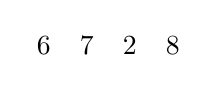
\begin{tikzpicture}[baseline=-.5em,scale=.42,line width=.8pt,line cap=round]
  \node at (0,0) {\rodten{6}}; \node at (1.3,0) {\rodunit{7}}; \node at (2.6,0) {\rodten{2}}; \node at (3.9,0) {\rodunit{8}};
\end{tikzpicture}}
\newcommand{\sqrttableA}{\begin{center}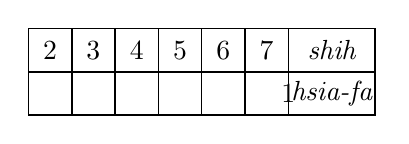
\begin{tikzpicture}[scale=.55,line width=.55pt]
\draw (0,0) rectangle (8,2);\foreach \x in {1,...,6}{\draw (\x,0)--(\x,2);}\draw (0,1)--(8,1);
\foreach \x/\t in {0.5/2,1.5/3,2.5/4,3.5/5,4.5/6,5.5/7}{\node at (\x,1.5){\t};}
\node[font=\itshape] at (7,1.5){shih};\node at (6,.5){1};\node[font=\itshape] at (7,.5){hsia-fa};
\end{tikzpicture}\end{center}}
\newcommand{\sqrttableB}{\begin{center}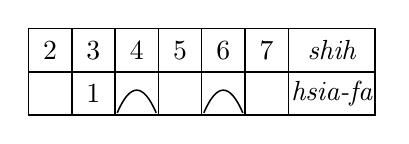
\begin{tikzpicture}[scale=.55,line width=.55pt]
\draw (0,0) rectangle (8,2);\foreach \x in {1,...,6}{\draw (\x,0)--(\x,2);}\draw (0,1)--(8,1);
\foreach \x/\t in {0.5/2,1.5/3,2.5/4,3.5/5,4.5/6,5.5/7}{\node at (\x,1.5){\t};}
\node[font=\itshape] at (7,1.5){shih};\node at (1.5,.5){1};\draw (2.05,.05)..controls(2.35,.75)and(2.65,.75)..(2.95,.05);\draw (4.05,.05)..controls(4.35,.75)and(4.65,.75)..(4.95,.05);\node[font=\itshape] at (7,.5){hsia-fa};
\end{tikzpicture}\end{center}}
\newcommand{\sqrttableC}{\begin{center}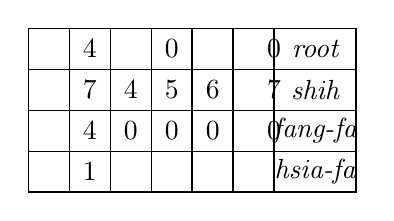
\begin{tikzpicture}[scale=.52,line width=.55pt]
\draw (0,0) rectangle (8,4);\foreach \x in {1,...,6}{\draw (\x,0)--(\x,4);}\foreach \y in {1,...,3}{\draw (0,\y)--(8,\y);} 
\node at (1.5,3.5){4};\node at (3.5,3.5){0};\node at (6,3.5){0};\node[font=\itshape] at (7,3.5){root};
\node at (1.5,2.5){7};\node at (2.5,2.5){4};\node at (3.5,2.5){5};\node at (4.5,2.5){6};\node at (6,2.5){7};\node[font=\itshape] at (7,2.5){shih};
\node at (1.5,1.5){4};\node at (2.5,1.5){0};\node at (3.5,1.5){0};\node at (4.5,1.5){0};\node at (6,1.5){0};\node[font=\itshape] at (7,1.5){fang-fa};
\node at (1.5,.5){1};\node[font=\itshape] at (7,.5){hsia-fa};
\end{tikzpicture}\end{center}}
\newcommand{\sqrttableD}{\begin{center}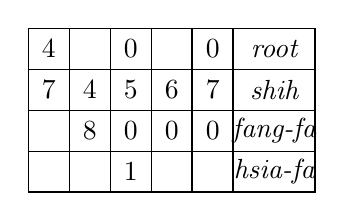
\begin{tikzpicture}[scale=.52,line width=.55pt]
\draw (0,0) rectangle (7,4);\foreach \x in {1,...,5}{\draw (\x,0)--(\x,4);}\foreach \y in {1,...,3}{\draw (0,\y)--(7,\y);} 
\node at (.5,3.5){4};\node at (2.5,3.5){0};\node at (4.5,3.5){0};\node[font=\itshape] at (6,3.5){root};
\node at (.5,2.5){7};\node at (1.5,2.5){4};\node at (2.5,2.5){5};\node at (3.5,2.5){6};\node at (4.5,2.5){7};\node[font=\itshape] at (6,2.5){shih};
\node at (1.5,1.5){8};\node at (2.5,1.5){0};\node at (3.5,1.5){0};\node at (4.5,1.5){0};\node[font=\itshape] at (6,1.5){fang-fa};
\node at (2.5,.5){1};\node[font=\itshape] at (6,.5){hsia-fa};
\end{tikzpicture}\end{center}}
\newcommand{\sqrttableE}{\begin{center}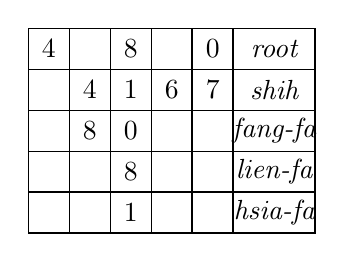
\begin{tikzpicture}[scale=.52,line width=.55pt]
\draw (0,0) rectangle (7,5);\foreach \x in {1,...,5}{\draw (\x,0)--(\x,5);}\foreach \y in {1,...,4}{\draw (0,\y)--(7,\y);} 
\node at (.5,4.5){4};\node at (2.5,4.5){8};\node at (4.5,4.5){0};\node[font=\itshape] at (6,4.5){root};
\node at (1.5,3.5){4};\node at (2.5,3.5){1};\node at (3.5,3.5){6};\node at (4.5,3.5){7};\node[font=\itshape] at (6,3.5){shih};
\node at (1.5,2.5){8};\node at (2.5,2.5){0};\node[font=\itshape] at (6,2.5){fang-fa};
\node at (2.5,1.5){8};\node[font=\itshape] at (6,1.5){lien-fa};
\node at (2.5,.5){1};\node[font=\itshape] at (6,.5){hsia-fa};
\end{tikzpicture}\end{center}}
\newcommand{\sqrttableF}{\begin{center}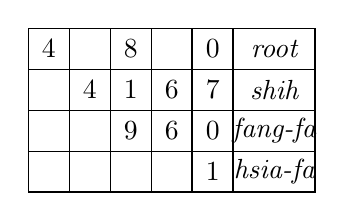
\begin{tikzpicture}[scale=.52,line width=.55pt]
\draw (0,0) rectangle (7,4);\foreach \x in {1,...,5}{\draw (\x,0)--(\x,4);}\foreach \y in {1,...,3}{\draw (0,\y)--(7,\y);} 
\node at (.5,3.5){4};\node at (2.5,3.5){8};\node at (4.5,3.5){0};\node[font=\itshape] at (6,3.5){root};
\node at (1.5,2.5){4};\node at (2.5,2.5){1};\node at (3.5,2.5){6};\node at (4.5,2.5){7};\node[font=\itshape] at (6,2.5){shih};
\node at (2.5,1.5){9};\node at (3.5,1.5){6};\node at (4.5,1.5){0};\node[font=\itshape] at (6,1.5){fang-fa};
\node at (4.5,.5){1};\node[font=\itshape] at (6,.5){hsia-fa};
\end{tikzpicture}\end{center}}
\newcommand{\sqrttableG}{\begin{center}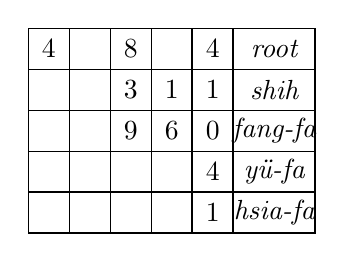
\begin{tikzpicture}[scale=.52,line width=.55pt]
\draw (0,0) rectangle (7,5);\foreach \x in {1,...,5}{\draw (\x,0)--(\x,5);}\foreach \y in {1,...,4}{\draw (0,\y)--(7,\y);} 
\node at (.5,4.5){4};\node at (2.5,4.5){8};\node at (4.5,4.5){4};\node[font=\itshape] at (6,4.5){root};
\node at (2.5,3.5){3};\node at (3.5,3.5){1};\node at (4.5,3.5){1};\node[font=\itshape] at (6,3.5){shih};
\node at (2.5,2.5){9};\node at (3.5,2.5){6};\node at (4.5,2.5){0};\node[font=\itshape] at (6,2.5){fang-fa};
\node at (4.5,1.5){4};\node[font=\itshape] at (6,1.5){yü-fa};
\node at (4.5,.5){1};\node[font=\itshape] at (6,.5){hsia-fa};
\end{tikzpicture}\end{center}}
\newcommand{\seaislandfig}{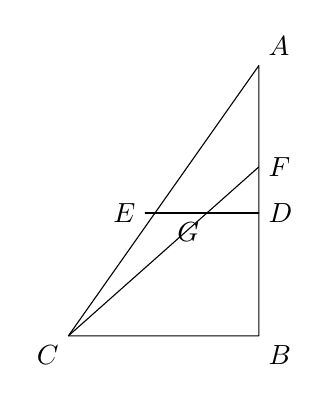
\begin{tikzpicture}[scale=.78,line cap=round,line join=round]
\coordinate (C) at (0,0);\coordinate (B) at (3.1,0);\coordinate (A) at (3.1,4.4);\coordinate (D) at (3.1,2.0);\coordinate (F) at (3.1,2.75);\coordinate (E) at (1.25,2.0);\coordinate (G) at (1.95,2.0);
\draw (C)--(B)--(A)--cycle;\draw (C)--(F);\draw (E)--(D);\node[above right] at (A){$A$};\node[below right] at (B){$B$};\node[below left] at (C){$C$};\node[left] at (E){$E$};\node[right] at (D){$D$};\node[right] at (F){$F$};\node[below] at (G){$G$};
\end{tikzpicture}}
\newcommand{\quadtable}{\begin{center}\begin{tabular}{|c|c|}\hline $-\left(c^2-\dfrac{r}{h}\times36\right)$&$x^0$\\\hline $c$&$x^1$\\\hline $1$&$x^2$\\\hline\end{tabular}\end{center}}
\renewcommand{\sqrttableA}{\begin{center}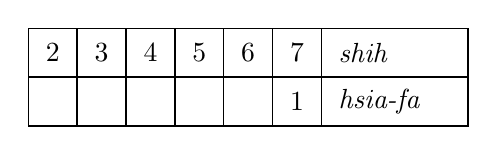
\begin{tikzpicture}[scale=.62,line width=.55pt]
\draw (0,0) rectangle (9,2);\foreach \x in {1,...,6}{\draw (\x,0)--(\x,2);}\draw (0,1)--(9,1);
\foreach \x/\t in {0.5/2,1.5/3,2.5/4,3.5/5,4.5/6,5.5/7}{\node at (\x,1.5){\t};}
\node[font=\itshape,anchor=west] at (6.15,1.5){shih};\node at (5.5,.5){1};\node[font=\itshape,anchor=west] at (6.15,.5){hsia-fa};
\end{tikzpicture}\end{center}}
\renewcommand{\sqrttableB}{\begin{center}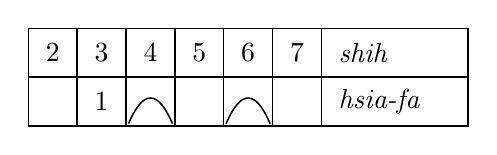
\begin{tikzpicture}[scale=.62,line width=.55pt]
\draw (0,0) rectangle (9,2);\foreach \x in {1,...,6}{\draw (\x,0)--(\x,2);}\draw (0,1)--(9,1);
\foreach \x/\t in {0.5/2,1.5/3,2.5/4,3.5/5,4.5/6,5.5/7}{\node at (\x,1.5){\t};}
\node[font=\itshape,anchor=west] at (6.15,1.5){shih};\node at (1.5,.5){1};\draw (2.05,.05)..controls(2.35,.75)and(2.65,.75)..(2.95,.05);\draw (4.05,.05)..controls(4.35,.75)and(4.65,.75)..(4.95,.05);\node[font=\itshape,anchor=west] at (6.15,.5){hsia-fa};
\end{tikzpicture}\end{center}}
\renewcommand{\sqrttableC}{\begin{center}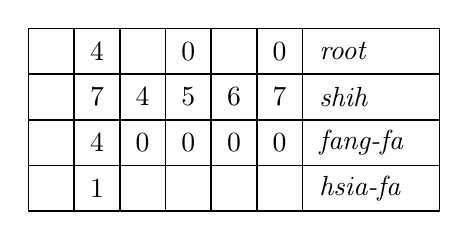
\begin{tikzpicture}[scale=.58,line width=.55pt]
\draw (0,0) rectangle (9,4);\foreach \x in {1,...,6}{\draw (\x,0)--(\x,4);}\foreach \y in {1,...,3}{\draw (0,\y)--(9,\y);} 
\node at (1.5,3.5){4};\node at (3.5,3.5){0};\node at (5.5,3.5){0};\node[font=\itshape,anchor=west] at (6.15,3.5){root};
\node at (1.5,2.5){7};\node at (2.5,2.5){4};\node at (3.5,2.5){5};\node at (4.5,2.5){6};\node at (5.5,2.5){7};\node[font=\itshape,anchor=west] at (6.15,2.5){shih};
\node at (1.5,1.5){4};\node at (2.5,1.5){0};\node at (3.5,1.5){0};\node at (4.5,1.5){0};\node at (5.5,1.5){0};\node[font=\itshape,anchor=west] at (6.15,1.5){fang-fa};
\node at (1.5,.5){1};\node[font=\itshape,anchor=west] at (6.15,.5){hsia-fa};
\end{tikzpicture}\end{center}}
\renewcommand{\sqrttableD}{\begin{center}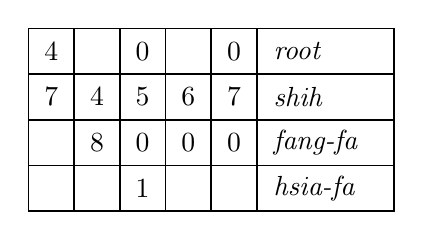
\begin{tikzpicture}[scale=.58,line width=.55pt]
\draw (0,0) rectangle (8,4);\foreach \x in {1,...,5}{\draw (\x,0)--(\x,4);}\foreach \y in {1,...,3}{\draw (0,\y)--(8,\y);} 
\node at (.5,3.5){4};\node at (2.5,3.5){0};\node at (4.5,3.5){0};\node[font=\itshape,anchor=west] at (5.15,3.5){root};
\node at (.5,2.5){7};\node at (1.5,2.5){4};\node at (2.5,2.5){5};\node at (3.5,2.5){6};\node at (4.5,2.5){7};\node[font=\itshape,anchor=west] at (5.15,2.5){shih};
\node at (1.5,1.5){8};\node at (2.5,1.5){0};\node at (3.5,1.5){0};\node at (4.5,1.5){0};\node[font=\itshape,anchor=west] at (5.15,1.5){fang-fa};
\node at (2.5,.5){1};\node[font=\itshape,anchor=west] at (5.15,.5){hsia-fa};
\end{tikzpicture}\end{center}}
\renewcommand{\sqrttableE}{\begin{center}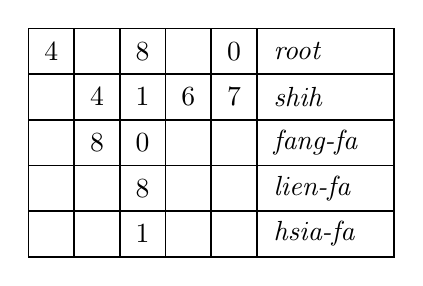
\begin{tikzpicture}[scale=.58,line width=.55pt]
\draw (0,0) rectangle (8,5);\foreach \x in {1,...,5}{\draw (\x,0)--(\x,5);}\foreach \y in {1,...,4}{\draw (0,\y)--(8,\y);} 
\node at (.5,4.5){4};\node at (2.5,4.5){8};\node at (4.5,4.5){0};\node[font=\itshape,anchor=west] at (5.15,4.5){root};
\node at (1.5,3.5){4};\node at (2.5,3.5){1};\node at (3.5,3.5){6};\node at (4.5,3.5){7};\node[font=\itshape,anchor=west] at (5.15,3.5){shih};
\node at (1.5,2.5){8};\node at (2.5,2.5){0};\node[font=\itshape,anchor=west] at (5.15,2.5){fang-fa};
\node at (2.5,1.5){8};\node[font=\itshape,anchor=west] at (5.15,1.5){lien-fa};
\node at (2.5,.5){1};\node[font=\itshape,anchor=west] at (5.15,.5){hsia-fa};
\end{tikzpicture}\end{center}}
\renewcommand{\sqrttableF}{\begin{center}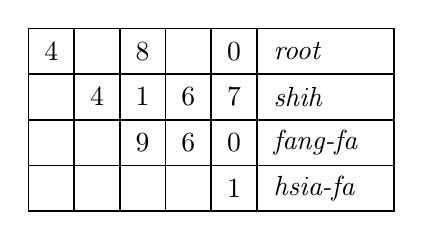
\begin{tikzpicture}[scale=.58,line width=.55pt]
\draw (0,0) rectangle (8,4);\foreach \x in {1,...,5}{\draw (\x,0)--(\x,4);}\foreach \y in {1,...,3}{\draw (0,\y)--(8,\y);} 
\node at (.5,3.5){4};\node at (2.5,3.5){8};\node at (4.5,3.5){0};\node[font=\itshape,anchor=west] at (5.15,3.5){root};
\node at (1.5,2.5){4};\node at (2.5,2.5){1};\node at (3.5,2.5){6};\node at (4.5,2.5){7};\node[font=\itshape,anchor=west] at (5.15,2.5){shih};
\node at (2.5,1.5){9};\node at (3.5,1.5){6};\node at (4.5,1.5){0};\node[font=\itshape,anchor=west] at (5.15,1.5){fang-fa};
\node at (4.5,.5){1};\node[font=\itshape,anchor=west] at (5.15,.5){hsia-fa};
\end{tikzpicture}\end{center}}
\renewcommand{\sqrttableG}{\begin{center}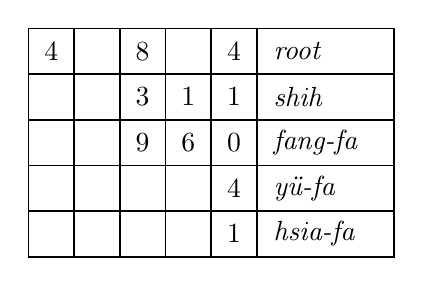
\begin{tikzpicture}[scale=.58,line width=.55pt]
\draw (0,0) rectangle (8,5);\foreach \x in {1,...,5}{\draw (\x,0)--(\x,5);}\foreach \y in {1,...,4}{\draw (0,\y)--(8,\y);} 
\node at (.5,4.5){4};\node at (2.5,4.5){8};\node at (4.5,4.5){4};\node[font=\itshape,anchor=west] at (5.15,4.5){root};
\node at (2.5,3.5){3};\node at (3.5,3.5){1};\node at (4.5,3.5){1};\node[font=\itshape,anchor=west] at (5.15,3.5){shih};
\node at (2.5,2.5){9};\node at (3.5,2.5){6};\node at (4.5,2.5){0};\node[font=\itshape,anchor=west] at (5.15,2.5){fang-fa};
\node at (4.5,1.5){4};\node[font=\itshape,anchor=west] at (5.15,1.5){yü-fa};
\node at (4.5,.5){1};\node[font=\itshape,anchor=west] at (5.15,.5){hsia-fa};
\end{tikzpicture}\end{center}}

\scanpage{0041}{Chapter 4, printed page 27}

ten thousands of ten thousands of one \emph{i} make one \emph{chao}, and so forth; while he counts thus: One \emph{hu} of the millet grains is six thousands of ten thousands; ten \emph{hu} are six \emph{i}, a hundred \emph{hu} are six \emph{chao}, etc.

Sun-Tsŭ takes $\pi=3$, and the ratio of the side and the diagonal of a square to be 5 to 7.

The weights of gold, silver, jewel, copper, lead, iron and stone are given to be one \emph{chin}, 14, 12, $7\frac{1}{2}$, $9\frac{1}{2}$, 6 and 3 \emph{liangs}, respectively, for one \emph{t'sun} cube.

Sun-Tsŭ does not explain expressly the use of the calculating pieces, but what he records in the first book of his treatise seems to indicate clearly the recourse being taken to that sort of abacus.

The calculating pieces are made of small bamboo or wooden pieces of two colours, red and black, representing the positive and the negative numbers. The pieces that were used in the later growth of mathematics were some $1\frac{1}{2}$ inches long and a sixth part of their length broad. But in old times much longer pieces made of bamboo were in use, as is recorded in the \emph{Han Shu}, written by Pan Ku at the end of the 1st Christian century. Although we are not certain how long the abacus had been used in China, yet we are sure that it was not first brought into use during the ages of the Han Dynasty; it had most likely been employed from time immemorial in China. A passage in the illustrious book, \emph{Tso Ch'uan}, serves to confirm this view; and the event told there relates to an occurrence in the year 542 B. C.

Sun-Tsŭ says in the first book of his treatise:

``In making calculations we must first know positions of numbers. Unity is vertical and ten horizontal; the hundred stands while the thousand lies; and the thousand and the ten look equally, and so also the ten thousand and the hundred.''

This stage in Sun-Tsŭ is nothing but a description of the arrangement of the calculating pieces. These pieces are usually arranged in the following manner:

The first five numbers are represented by 1, 2, 3, 4 and 5 of these pieces, that are arranged vertically, while in the arrangement of the numbers from 6 to 9 one piece taken in the horizontal position over other vertical pieces is taken for 5. Thus:

\begin{center}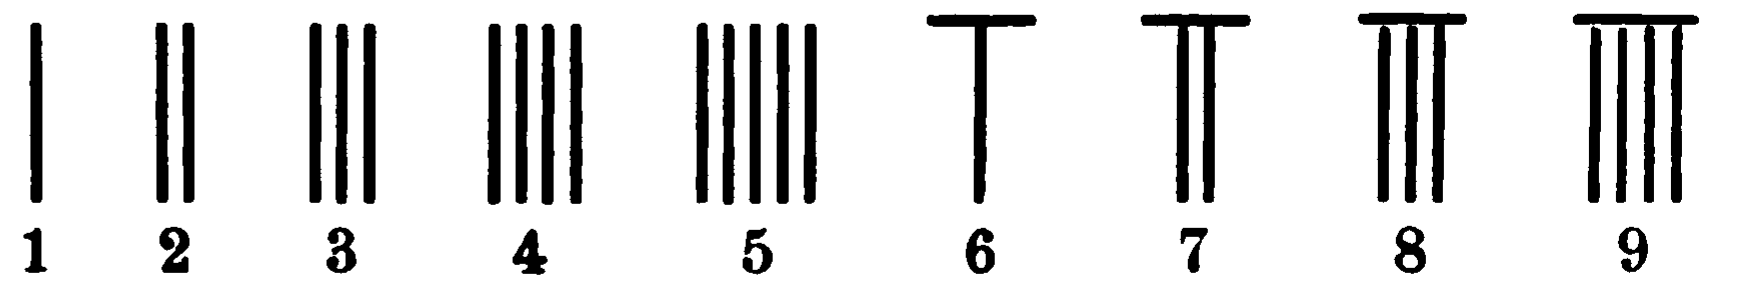
\includegraphics[width=.70\linewidth]{pdf041-rod-numerals-units.png}\end{center}

This way of arrangement is referred to in Sun-Tsŭ's work in the paragraph that follows that which we have just quoted; and it is also
\scanfooter

\scanpage{0042}{Part I, printed page 28}

in sound accordance with what we can conjecture from the obscure passage in the \emph{Tso Ch'uan} mentioned above. Moreover, this was the very way that was followed in subsequent ages.

The figures in the ten's column are arranged with the calculating pieces in the following manner:

\begin{center}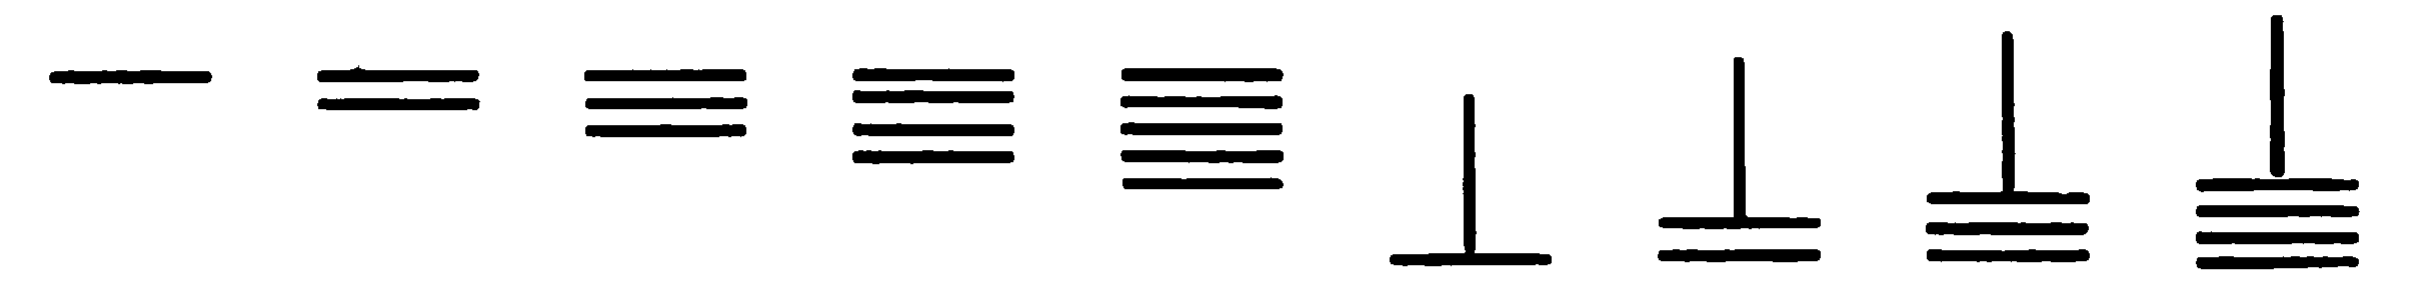
\includegraphics[width=.86\linewidth]{pdf042-rod-numerals-tens.png}\end{center}

For hundreds and higher numbers these arrangements are repeated alternately, but nothing new comes in. Thus the number 6728 will be arranged as annexed.

\begin{center}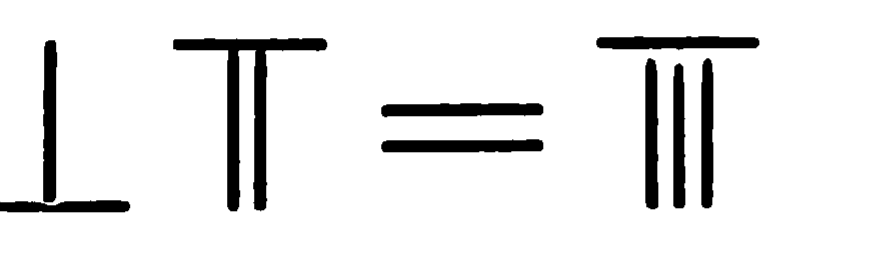
\includegraphics[width=.32\linewidth]{pdf042-rod-number-6728.png}\end{center}

To multiply two numbers together, Sun-Tsŭ directs to arrange these numbers in superposition upper and lower, in such a way that the unit in the lower number should come just underneath the highest digit in the upper number. That highest digit should first be multiplied by the lower number, when the partial product thus obtained should be arranged in a line that comes between the two. Then the highest digit in the upper number should be striken out, and the number underneath is to be drawn back by one digit. And now the second highest digit in the upper number should be multiplied by the lower number, the partial product being entered in the middle line, which is thus rectified. This rectification is not very difficult because the numbers are all arranged with movable pieces. Proceeding in this way the final answer will be obtained at the end of the process.

In division, as stated by Sun-Tsŭ, unlike the case of multiplication, the quotient is not arranged in the middle line, or between the dividend and the divisor, but in the topmost line. For instance, to divide 100 by 6, these numbers are arranged in superposition, the divisor coming below the other. Advance the divisor, in this case, by two positions or columns so as to bring it under the hundred's position, and try the division. But 1 is not divisible by 6, because the divisor is greater than the dividend. Hence drawing back to the ten's position, and arranging 1 for the quotient in the uppermost line, we multiply it by the divisor in the lowest line, and we are able to strike out $1\times 6=6$ from the dividend. Then the divisor is to be drawn back by one column, and we proceed in like manner. When there is a remainder after the division is over, take the quotient of this remainder divided by the divisor as the fractional part of the quotient.
\scanfooter

\scanpage{0043}{Chapter 4, printed page 29}

The division with a divisor that is of more than one digits is not explained in the Classic of Sun-Tsŭ, though it contains a number of such examples.

Fractions are treated in the second book of Sun-Tsŭ.

The reduction of a fraction to the simplest form is done by finding the greatest common measure of the two members, which is the same as we find in the ``Arithmetic in Nine Sections''. But Sun-Tsŭ states that the denominator should be arranged in the lower line and the numerator in the upper line.

In adding two fractions Sun-Tsŭ indicates that the denominators should be arranged in the right and the numerators in the left, and that then the denominators should be cross multiplied into the numerators, the sum of which products makes the numerator and the product of the denominator in the right column makes the denominator of the resulting fraction.

Sun-Tsŭ takes the area of a circle to be $\dfrac{c}{2}\times\dfrac{d}{2}$, $\dfrac{c^2}{12}$, or $d^2\times\dfrac{3}{4}$, where $d$ and $c$ denote the diameter and circumference.

The explanation of the extraction of the square-root found in the second book of Sun-Tsŭ, although little differing from that in the ``Nine Sections'', is exceedingly clear in meaning, unlike the obscure language in the latter. The technical terms used here were the same that became current both in China and in Japan in later years, if not in the same meanings as uesd by Sun-Tsŭ. We shall therefore try to quote from the text the following rule:

``Arrange the area 234567 paces square and make it the \emph{shih}.

``Next borrow a unit calculator, and make it the \emph{hsia-fa}.''\footnote{The word \emph{hsia} means below or under.}

Thus

\begin{center}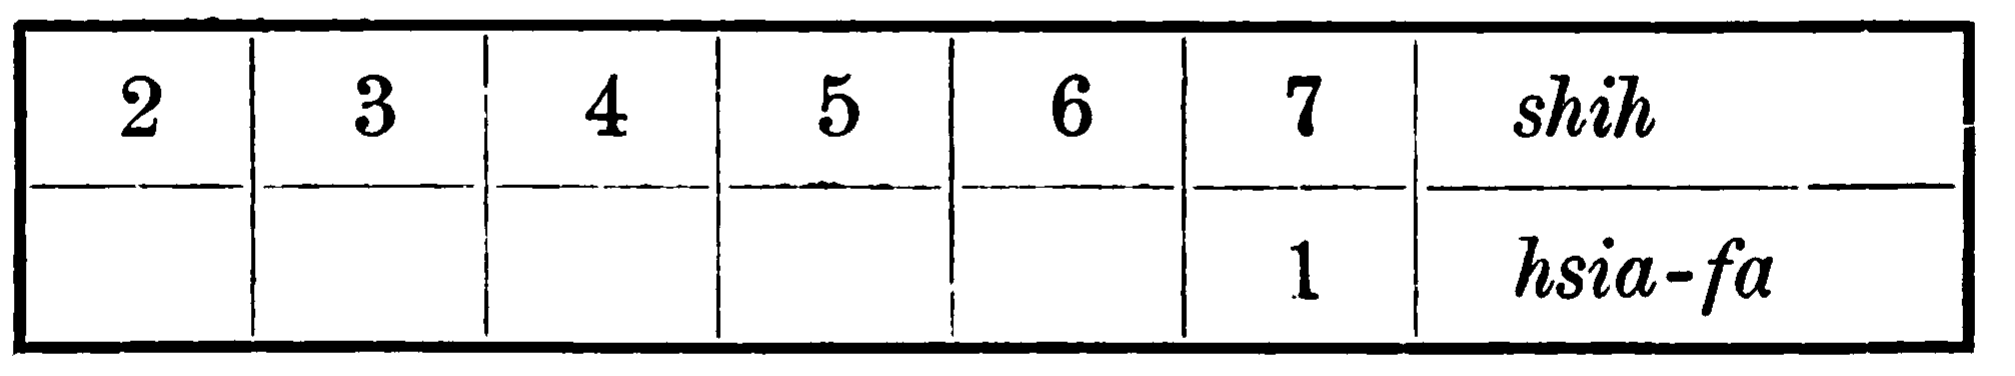
\includegraphics[width=.80\linewidth]{pdf043-sqrt-table-a.png}\end{center}

``Advance it over every one column, thus dividing the \emph{shih} in groups, until it reaches the hundred's place.'' Thus:

\begin{center}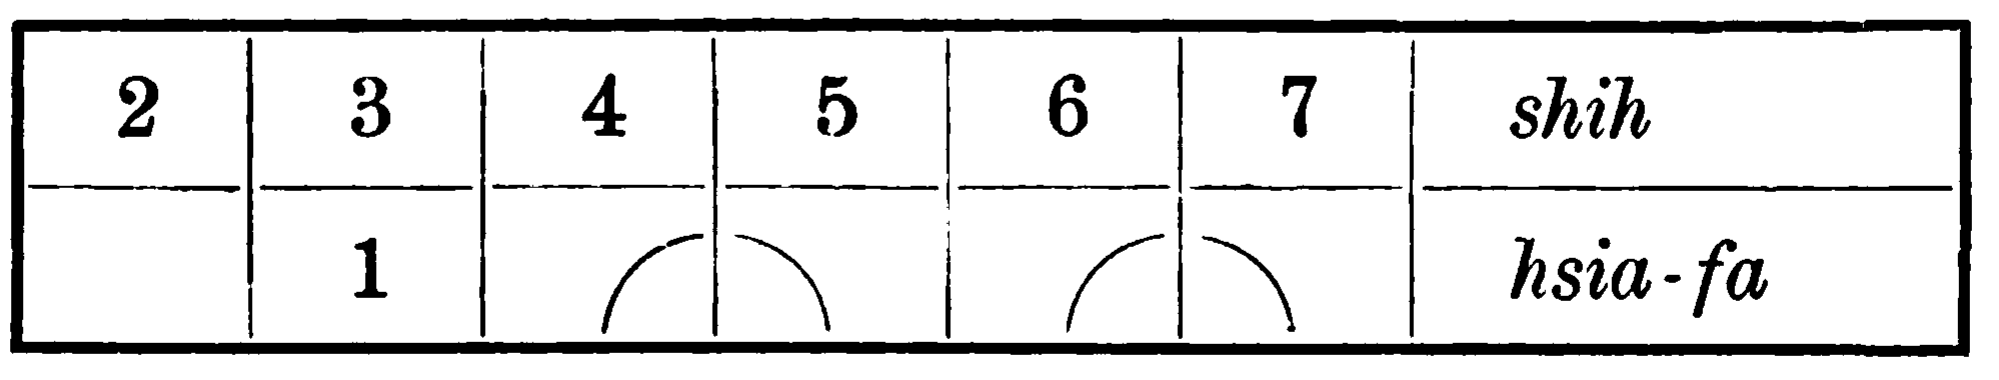
\includegraphics[width=.80\linewidth]{pdf043-sqrt-table-b.png}\end{center}

``Arrange the \emph{shang} or root 400 above the \emph{shih}.
\scanfooter

\scanpage{0044}{Part I, printed page 30}

``Subjoin 40000\footnote{This is the product of the root and the \emph{hsia-fa}.} under the \emph{shih} and above the \emph{hsia-fa}, and make it the \emph{fang-fa}.

``With it multiply the root 400 and subtract the product from the \emph{shih}.'' Thus:

\begin{center}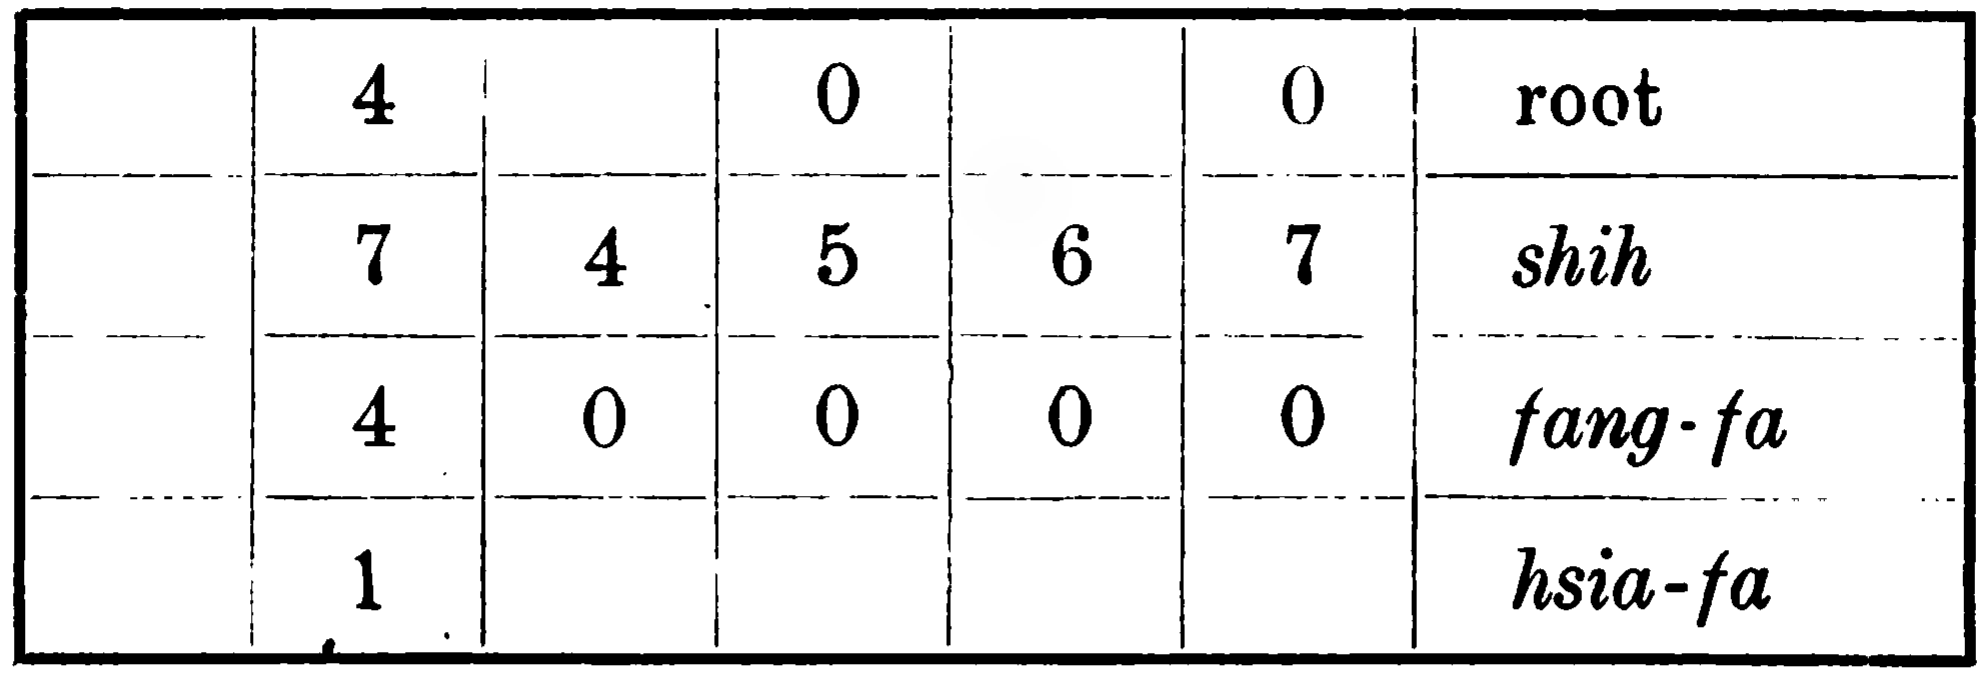
\includegraphics[width=.72\linewidth]{pdf044-sqrt-table-c.png}\end{center}

``The subtraction being done, double the \emph{fang-fa}, and draw it back one column, and the \emph{hsia-fa} two columns.'' Thus:

\begin{center}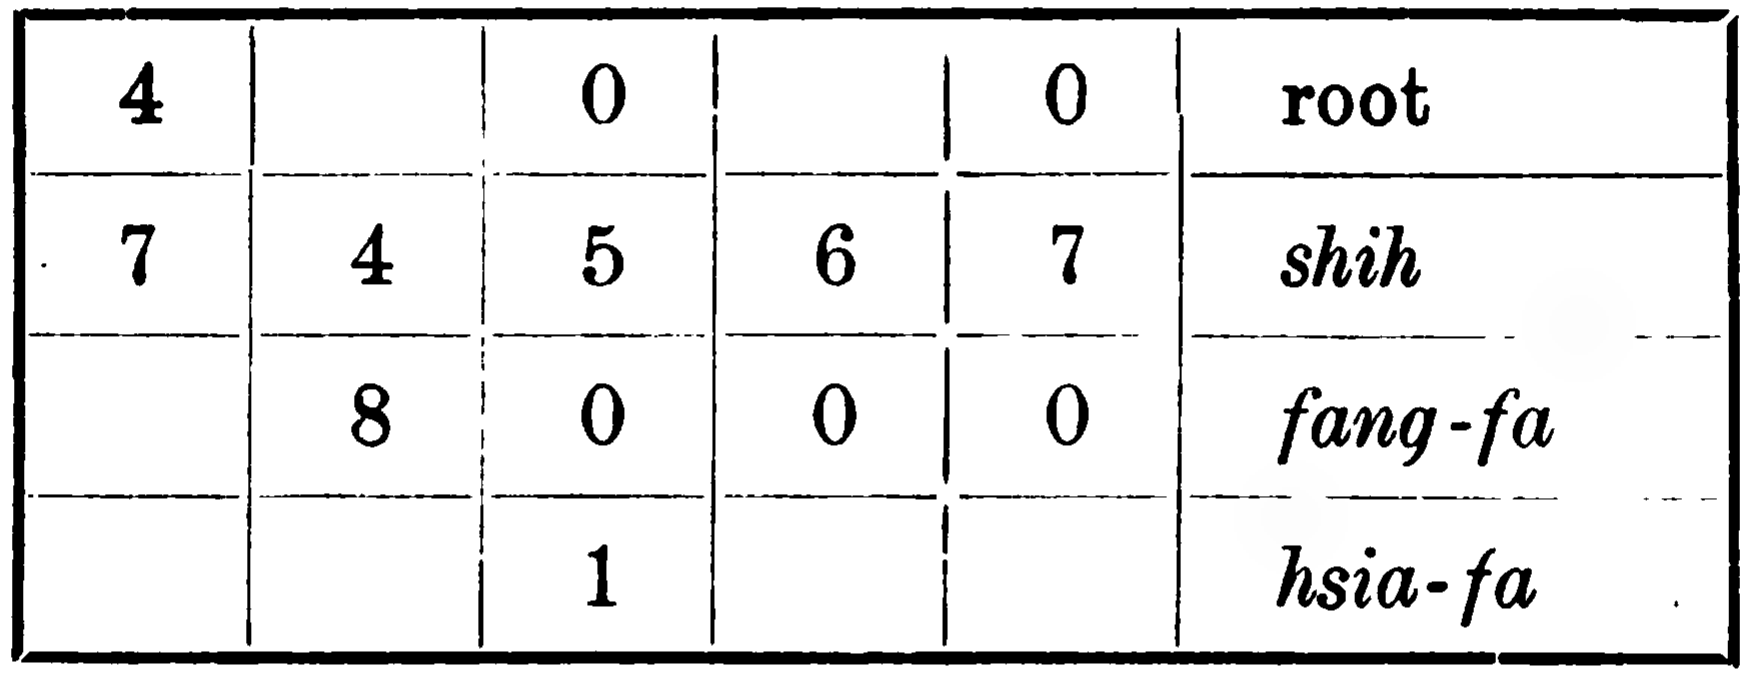
\includegraphics[width=.64\linewidth]{pdf044-sqrt-table-d.png}\end{center}

``Again arrange 80 for the root next to the previous digit.

``Subjoin 800 under the \emph{fang-fa} and above the \emph{hsia-fa}; nominate it the \emph{lien-fa}.

``Multiply the \emph{fang-fa} and the \emph{lien-fa} by the root 80, and subtract the products from the \emph{shih}.'' Thus:

\begin{center}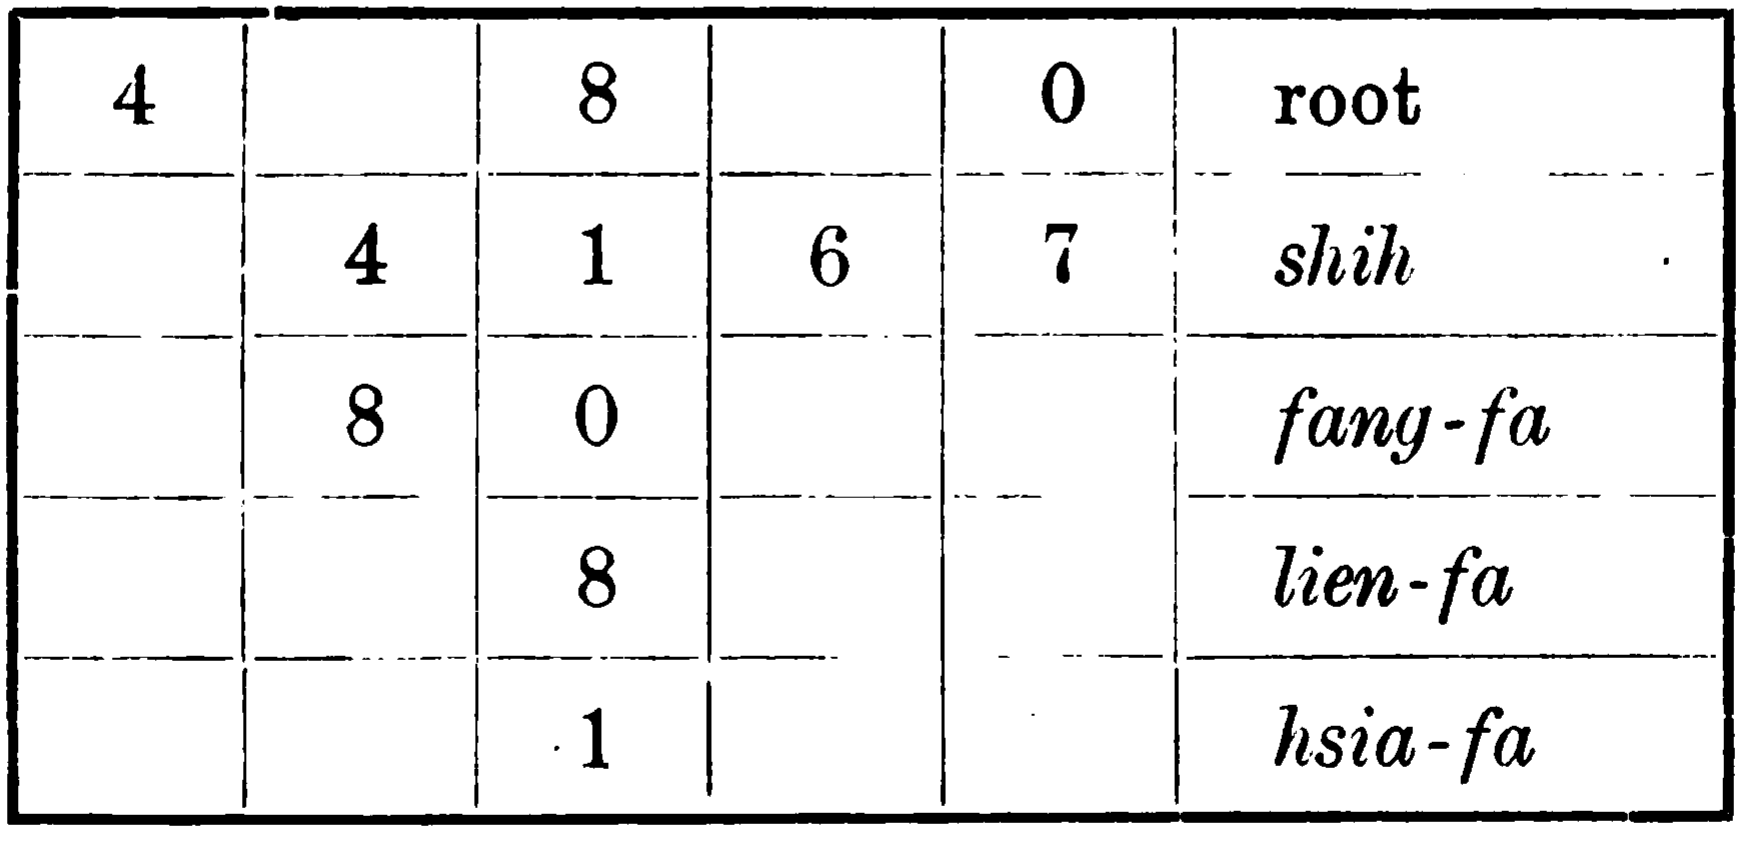
\includegraphics[width=.64\linewidth]{pdf044-sqrt-table-e.png}\end{center}

``When these subtractions are done, double the \emph{lien-fa}, and add to the \emph{fang-fa}.

``Draw back the \emph{fang-fa} one column, and the \emph{hsia-fa} two columns.''
\scanfooter

\scanpage{0045}{Chapter 4, printed page 31}

Here the \emph{lien-fa} is understood to be got rid of. And thus the arrangement becomes:

\begin{center}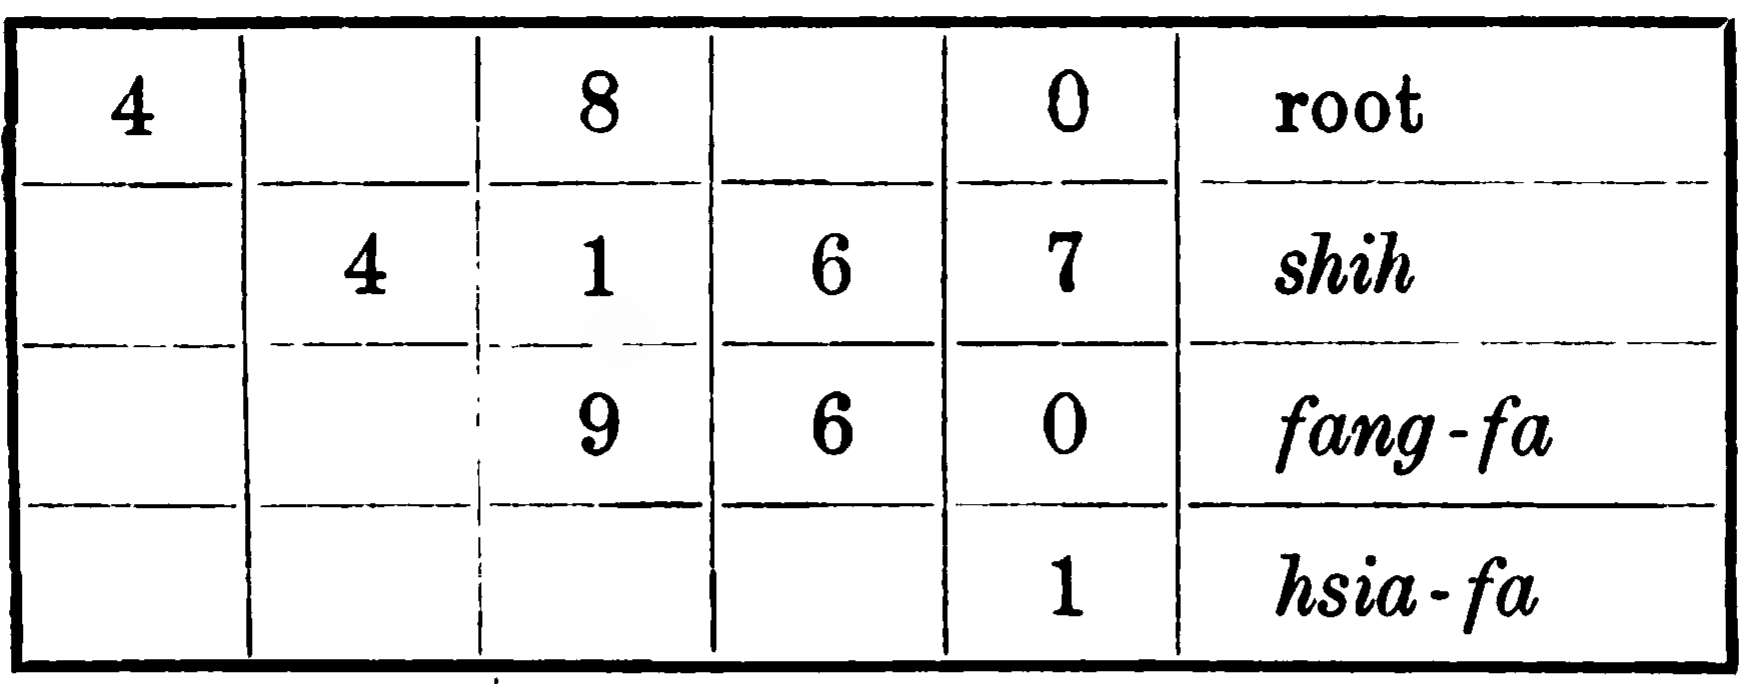
\includegraphics[width=.70\linewidth]{pdf045-sqrt-table-f.png}\end{center}

``Again, arrange 4 in the next column of the previous root.

``Subjoin 4 under the \emph{fang-fa} and above the \emph{hsia-fa}, and name it the \emph{yü-fa}.\footnote{This is the same as the previous \emph{lien-fa}, only that it is differently named.}

``Multiply the \emph{fang}, \emph{lien}, and \emph{yü}\footnote{This passage may seem somewhat strange, but it means that the \emph{fang-fa} and the \emph{yü-fa} are to be multiplied by 4 in the root.} by the root 4, and subtract the products from the \emph{shih}.'' Thus:

\begin{center}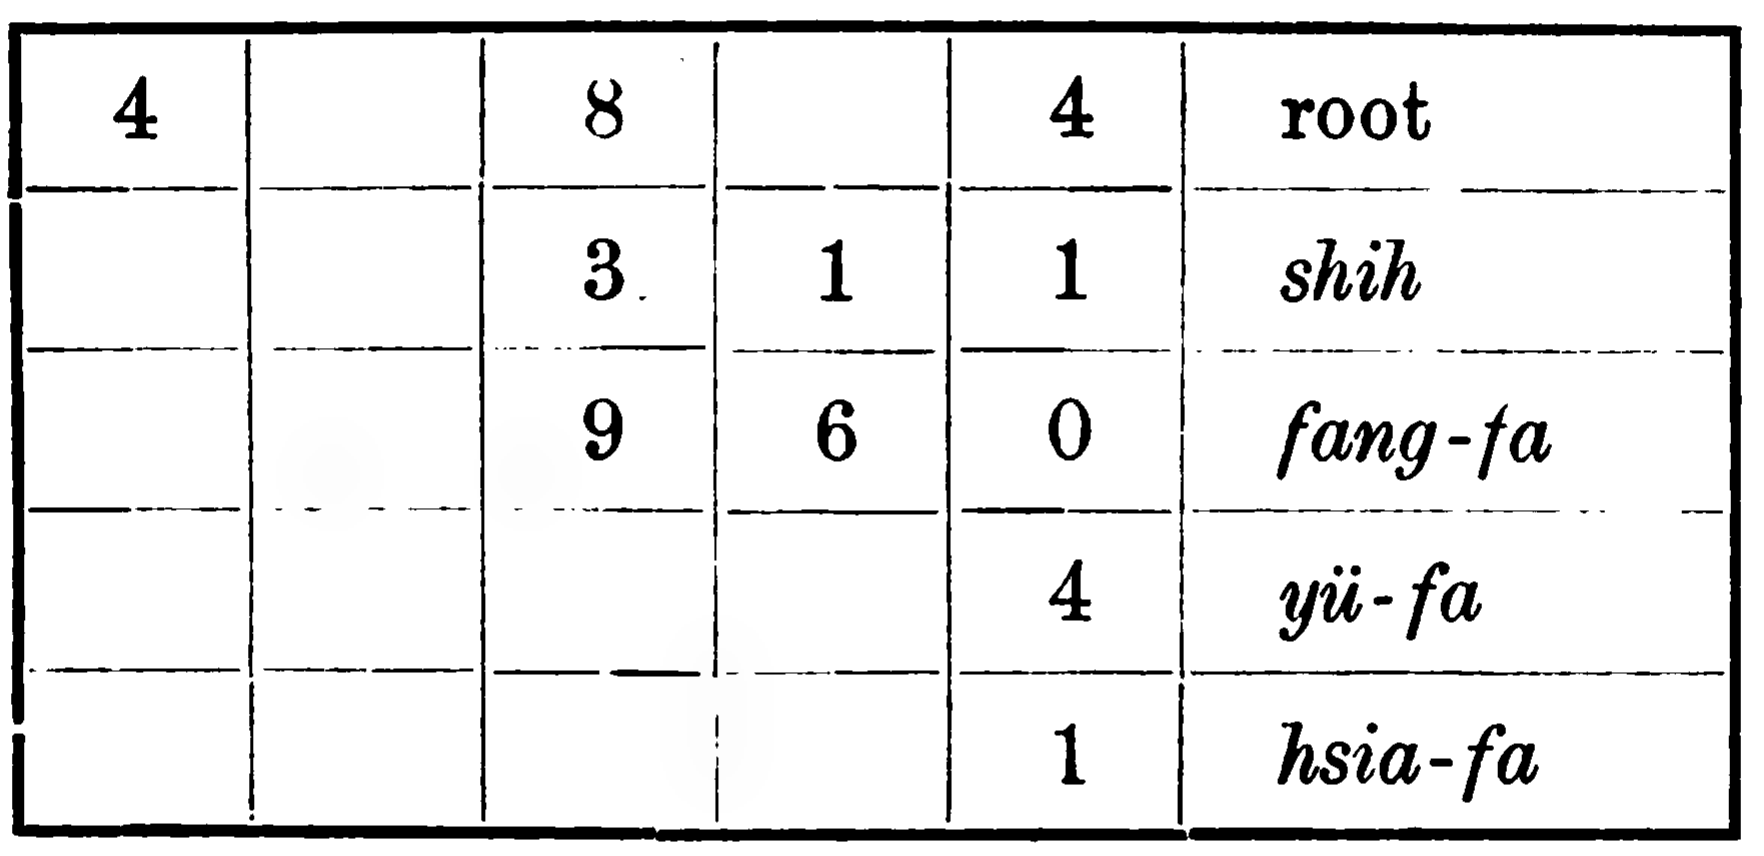
\includegraphics[width=.70\linewidth]{pdf045-sqrt-table-g.png}\end{center}

``This being over, double the \emph{yü-fa} and add it to the \emph{fang-fa}.

``Thus we get 484 for the root in the above and 968 for the \emph{hsia-fa}\footnote{This is not in the same meaning as previously.}, the remainder being 311.''

``One side (of the square) is therefore $484\,\dfrac{311}{968}$ paces.''

This last step, that had been also adopted in the ``Nine Sections'', appears to have been invariably followed by all the mathematicians of ancient China.

Sun-Tsŭ does not consider the case of the cube root.

We here state one or two problems from Sun-Tsŭ's ``Arithmetical Classic'', Book 3.

``A woman was washing dishes in a river, when an official whose business was overseeing the waters demanded of her: `Why are there so
\scanfooter

\scanpage{0046}{Part I, printed page 32}

many dishes here?' --- `Because a feasting was entertained in the house', the woman replied. Thereupon the official inquired of the number of the guests. `I don't know', the woman said, `how many guests had been there; but every two used a dish for rice between them; every three a dish for broth; every four a dish for meat; and there were sixty-five dishes in all.''

``Rule. Arrange the 65 dishes, and multiply by 12, when we get 780. Divide it by 13, and thus we obtain the answer.''

``There are certain things whose number is unknown. Repeatedly divided by 3, the remainder is 2; by 5 the remainder is 3; and by 7 the remainder is 2. What will be the number?''

This problem reduces to the indeterminate equations
\[
3m_1+2=5m_2+3=7m_3=2,
\]
of which the solution is
\[
m_1=5\times7r+7,\qquad m_2=21r+4,\qquad m_3=3\times5r+3,
\]
for $r=0,1,2,3,\ldots$.

Sun-Tsŭ tries to solve this problem thus:

``The remainder divided by 3 is 2, and so take 140. The remainder divided by 5 is 3, and so take 63. The remainder divided by 7 is 2, and so take 30. Adding these together we get 293. Therefrom subtract 210, and we obtain the answer.''

Sun-Tsŭ thus satisfied himself with a single solution of the problem.

Further adds Sun-Tsŭ: ``In general, take 70, when the remainder of the repeated divisions by 3 is 1; take 21, when the remainder of the repeated divisions by 5 is 1; and take 15, when the remainder of the repeated divisions by 7 is 1. When the sum of these numbers is above 106, subtract 105, before we get the answer.''

All the subjects treated by Sun-Tsŭ were those that had been given in the ``Arithmetic in Nine Sections'', but the problem of indeterminate analysis first appeared in the above in Sun-Tsŭ.

In solving what is equivalent to the simultaneous system
\[
2x+1y=96,\qquad 2x+3y=144,
\]
Sun-Tsŭ tries to multiply these equations respectively by the coefficients of $x$ in the other, and carry out the mutual subtraction. See how he adheres to form; but see how here a step has been obtained in advance of the ``Nine Sections'' by mutually multiplying the coefficients by each other.
\scanfooter

\scanpage{0047}{Chapter 4, printed page 33; opening of Chapter 5}

We find in Sun-Tsŭ a problem of finding the least common multiple. It is this:

``There are three sisters, of whom the eldest comes home once in every 5 days, the middle in every 4 days, and the youngest in every 3 days. In how many days will all the three meet together?''

The answer is 60 days.

To solve it Sun-Tsŭ gives the rule in these words:

``Arrange the 5 days of the eldest sister, the 4 days of the middle and the 3 days of the youngest in the right column. Opposite to each of these arrange unity on the left column. Then cross multiply (the numbers on the right), when we get the numbers of their returning. Thus the eldest comes 12 times, the middle 15 times and the youngest 20 times. If we multiply these numbers by the numbers of days in which the sisters once come back, we shall obtain the desired answer.''

The last problem in the ``Arithmetical Classic'' of Sun-Tsŭ is one that relates to fortune-telling. Thus:

``A pregnant woman, who is 29 years of age, is expected to give birth to a child in the 9th month of the year. Which should be her child, a son or a daughter?''

Sun-Tsŭ gives to this problem the rule:

``Take 49; add the month of her child-bearing; subtract her age. From what now remains, subtract the heaven 1, subtract the earth 2, subtract the man 3, subtract the four seasons 4, subtract the five elements 5, subtract the six laws 6, subtract the seven stars 7, subtract the eight winds 8, subtract the nine provinces 9. If then the remainder be odd, the child shall be a son; and if even, a daughter.''

Yüan Yüan desires in his ``Biographical Collections'' to ascribe this one problem to a subsequent addition, not to the original text of Sun-Tsŭ, since it appears to him too unbecoming for so able a writer as Sun-Tsŭ.

\begin{center}
CHAPTER 5.\par
\medskip
THE HAI-TAO SUAN-CHING OR THE SEA-ISLAND\par
ARITHMETICAL CLASSIC.
\end{center}
\phantomsection\addcontentsline{toc}{subsection}{Chapter 5. The Hai-Tao Suan-Ching or the Sea-Island Arithmetical Classic}

The \emph{Hai-tao Suan-ching} or literally the ``Sea-Island Arithmetical Classic'' was a treatise written by Liu Hui, who belonged to the Kingdom of Wei at the warlike period of the Three Monar-

\scanfooter

\scanpage{0048}{Part I, printed page 34}

chies.\footnote{The age of the Three Monarchies begins with the collapse of the Later Han Dynasty in the beginning of the 3rd century A. D., and lasted for half a century. The three monarchies are Wei in the north, Wu in the south, and Shih in the west. The Kingdom of Wei was exterminated in the year 265, when the Dynasty of Chin rose in power.} The title of the ``Sea-island Arithmetical Classic'' was not the one originarilly applied by the author himself. Liu Hui commented on the ``Arithmetic in Nine Sections'', as we have said, when he worked the solutions of some problems which he classified under the heading of \emph{Chung-ch'a}, and added next to the chapter on the \emph{Kou-ku}, the last of the nine sections. But Liu's additions could not constitute the text of the ``Nine Sections'', and it was destined in course of time to be considered separately, assuming the title it now illustriously bears. The title originated, because the first problem in the book concerns the measurement of an island from a distance; it has been used perhaps from the beginning of the T'ang Dynasty, which arose to ascendency in the 7th century.

There has remained no proper copy of Liu Hui's work; it was only preserved in the manuscripts bearing the title, \emph{Yung-lo Tai-tien}, composed in the \emph{Yung-lo} Era (1403--1424) by the Ming government. The ``Sea-island Arithmetical Classic'', as we now possess it, was collected by the imperial librarian and mathematician, Tai Chêng, in 1775 from among the great collections just mentioned. The book is provided with the commentaries of Li Ch'un-fêng, who flourished at the middle of the 7th century.

About Liu Hui's life we know little or nothing, except that he wrote his commentary on the ``Arithmetic in Nine Sections'' in the year 263 A. D., under the reign of Ch'ên-liu-Wang of the Wei Kingdom, as we learn from the \emph{Chin Shu} or the ``Records of the Chin Dynasty''. If there be some different opinions about Liu's date, yet we cannot but believe that the accounts in the ``Chin Records'' are the most authentic.

The first problem in the ``Sea-island Arithmetical Classic'' is this:

``There is a sea-island that is to be measured. Two rods that are both 30 feet ($a$) high are erected at the distance of 1000 paces ($b$) from each other, making the rod in the rear to come in the same straight line with the island and the other rod. When a man walks 123 paces ($c$) back from the nearer rod, the top of the island is just visible through the end of that rod, if he tries to see with his eye brought on the ground. The summit of the island peak is also seen
\scanfooter

\scanpage{0049}{Chapter 5, printed page 35}

costraight with the end of the hind rod, when seen bringing the eye in contact with the ground from a point 127 paces ($d$) back from that rod. It is required to know the height and the distance of the island.''

The rule given for the solution of this problem runs:

``Rule. With the height of the rods multiply the distance of the rods, and take (the product) as the dividend; and carry the division taking the difference (of the distances walked back from the rods) as the divisor; add to the quotient the rod's height, when we obtain the height of the island.

``To find the distance of the island from the nearer rod, multiply with the distance walked back from that rod the distance between the two rods, and divide the product by the difference of the distances walked back from the rods, when the quotient gives the distance required.''

This rule is equivalent to the formulae,
\[
(\text{height})=a+\frac{ab}{d-c};\qquad (\text{distance})=\frac{cb}{d-c}.
\]

It is not known how Liu Hui got at these expressions, but it appears not improbable that they were deduced from the two proportions,
\[
\frac{x}{x+c}=\frac{a}{c},\qquad \text{and}\qquad \frac{x}{x+b+d}=\frac{a}{d},
\]
or what are equivalent to them.

The term \emph{chung-ch'a} seems to indicate an agreement with our view. The term was originally intended to mean double or repeated applications of the consideration as met with in the chapter on the right triangle in the ``Nine Sections'', i. e., the double application of proportions.

The second of Liu Hui's problems is as follows:

``There grows on a hill a pine-tree, whose height is not known. Two rods, each 20 feet high ($a$), are so erected in the plain below at the mutual distance of 50 paces ($b$), that they come in a straight line with the tree. The top of the tree and the end of the front rod make a straight line with a point on the ground 7 paces and 4 feet ($c$) behind the rod, and at this point the base of the tree measures 2.8 feet ($e$) on the top of the rod. The top of the tree again makes a straight line with the end of the hind rod and a point on the ground 8 paces and 5 feet ($d$) behind the rod. It is required to know the height of the pine-tree and the distance of the hill from the (front) rod.''
\scanfooter

\scanpage{0050}{Part I, printed page 36; end of Chapter 5}

The rule that is intended to solve this problem leads to the formulae,
\[
(\text{height})=\frac{eb}{d-c}+e;\qquad (\text{distance})=\frac{bc}{d-c}.
\]

The third problem is:

``One sees to the south a square town of unknown size. He erects two rods 60 feet ($a$) apart from east to west, which are joined with a string at the eye's height, and let the eastern rod be costraight with the S. E. corner and the N. E. corner of the town.

\begin{center}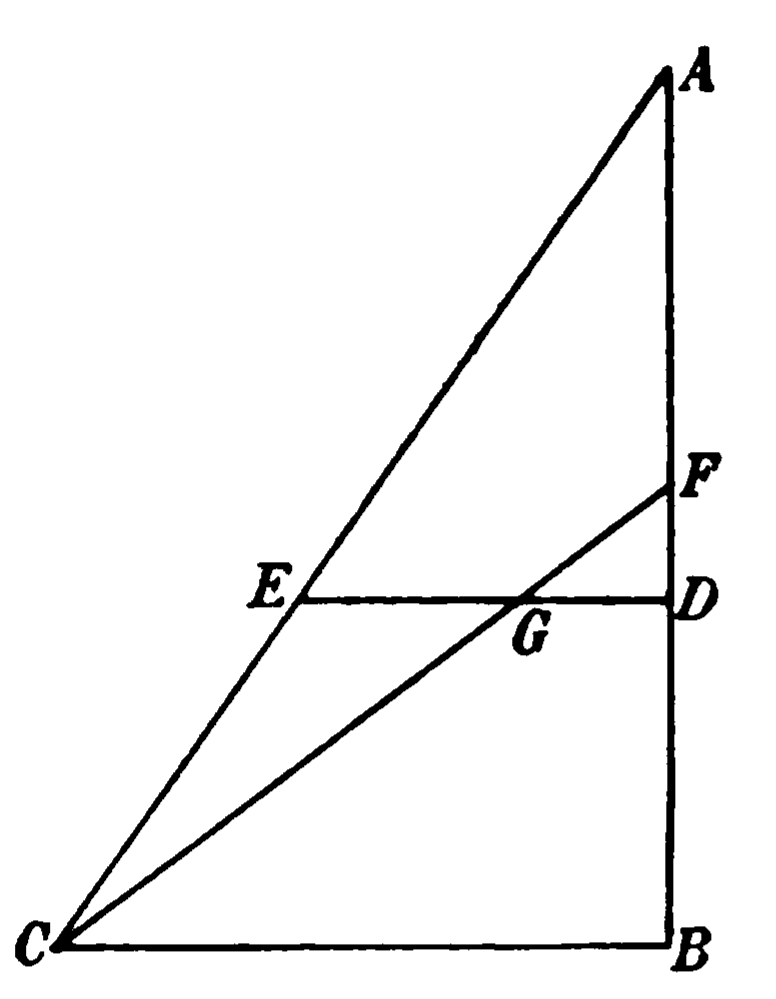
\includegraphics[width=.28\linewidth]{pdf050-square-town-diagram.png}\end{center}

He gets 5 paces ($b$) to the north of the eastern rod, and observes the N. W. corner of the town through a point of the string at $22\cdot6\frac{1}{2}$ feet ($c$) from the east end. Again getting back to the north 13 paces and 2 feet ($d$) from the rod, the observer sees the N. W. corner of the town just costraight with the western rod. What are then one side of the town and the distance of the town from the rod?''

This problem is the same as asking for the lengths (see the figure) $CB=x$ and $BD=y$ in terms of $DE=a$, $DF=b$, $DG=c$, $DA=d$. [In the figure $B$ is a right angle and $DE$ is drawn parallel to $BC$.]

The formulae in the answer are given in forms equivalent to
\[
x=\frac{(d-b)c}{\dfrac{cd}{a}-b},\qquad
 y=\frac{\left(d-\dfrac{cd}{a}\right)b}{\dfrac{cd}{a}-b}.
\]

Liu Hui gives in his ``Arithmetical Classic'' six further similar problems, together with the rules for their solutions.

Liu Hui's studies of these complicated problems appear to tell that he was acquainted with some way of algebraical manipulations. When we moreover reflect on the contents of some parts of the ``Nine Sections'', we cannot but ascribe the birth of algebra to Chinese mathematicians in a comparatively early part of their history, much earlier than the time of the appearance of Ch'in Chiu-shao and Li Yeh in the 13th century, when, as is generally believed, the Chinese algebra was born. We put therefere a stress on Liu Hui's considerations of these complicated problems, that had taken place in the 3rd century, a whole millenium previous to the dawning of the algebra of the celestial element, of which we shall have to consider something later on.
\scanfooter

\scanpage{0051}{Chapter 6, printed page 37}
\begin{center}
CHAPTER 6.\par
\medskip
THE WU-T'SAO SUAN-CHING AND THE WORKS OF HSIA-HOU\par
YANG, CHANG CH'IU-CHIEN AND CHÊN LUAN.
\end{center}
\phantomsection\addcontentsline{toc}{subsection}{Chapter 6. The Wu-T'sao Suan-Ching and the Works of Hsia-Hou Yang, Chang Ch'iu-Chien and Chên Luan}

What we have next to describe are the arithmetical classics that were adopted by the T'ang government as the treatises in its vast examination system for the election of civil officers, and that are still extant, other than those of which we have already made our reviews. We mean namely the \emph{Wu-t'sao Suan-ching} and the works of Hsia-hou Yang, Chang Ch'iu-chien and Chên Luan.

Of these the author of the \emph{Wu-t'sao Suan-ching} is not known; this title was given to the work, perhaps because it contains five books or chapters treating under so many different headings. Its date of composition is also unknown. So also are all lost the dates of the two mathematicians Hsia-hou Yang and Chang Ch'iu-chien. But Hsia-hou speaks in the preface to his treatise thus:

``But the arithmetic dawned from the time of Fu-hi, and the Yellow Emperor\footnote{The Yellow Emperor belonged to the 27th century B. C.} regulated the three numbers and made the ten degrees\footnote{These are understood to be something in arithmetical considerations.}, when Li-Shou thereby worked the ``Nine Sections''. \ldots{} After the \emph{Wu-t'sao} and Sun-Tsŭ, there have been various arithmetical treatises, and Chên Luan and Liu Hui wrote detailed commentaries on these books. \ldots{}''

Chang Ch'iu-chien states expressly in the preface to his work that he changes some of the solutions of Hsia-hou Yang and of Sun-Tsŭ, which he actually does in the text of his book.

It therefore appears that Sun-Tsŭ and the \emph{Wu-t'sao Suan-ching} belong to the earliest dates, certainly to the age of the Dynasties of Han, Former or Later, the works of Hsia-hou and Chang appearing in subsequent ages. When we reflect however on the fact that Chang's ``Arithmetical Classic'' was commented upon by Chên Luan, although these commentaries of Chên are now lost, and that Hsia-hou speaks of the commentaries of Liu Hui and Chên Luan upon the works of Sun-Tsŭ and the \emph{Wu-t'sao Suan-ching}, it must be concluded that the two authors Hsia-hou and Chang were doubtlessly both contemporaries of Chên Luan. Moreover, according to Yüan Yüan\footnote{Yüan's \emph{Biographical Notices}, Book 11.}, Chên Luan even wrote a commentary on the ``Arithmetical Classic'' of Hsia-hou Yang.
\scanfooter

\scanpage{0052}{Part I, printed page 38}

Hsia-hou writes in the text of his treatise that the standard of the measure of volume had been reconstructed in the year 425, and again by Chên Luan in 535. It is well known that Chên Luan served Wu-Ti, emperor of Chou, as a minister in the second half of the 6th century. He was extraordinarily enthusiastic in favouring Buddhism against the persecutions. Chên Luan's \emph{Wu-ching Suan-shu} was a composition under the reign of the Monarchy of Chou, for he signs in it as belonging to the Dynasty, a monarchy that sprung into existence in 557 and was overthrown in 581.

The mathematical treatises under consideration, except the \emph{Wu-t'sao}, belong therefore safely to the 6th century.

We shall first describe the oldest of these treatises, or the \emph{Wu-t'sao Suan-ching}.

There are some problems in this work, whose rules of solution appear odd and unintelligible. These are taken as erroneous by later scholars.

For instance the areas of ``drum-shaped'' fields, whose form probably consists of two congruent equilateral trapezoids, whose two equal bases, the greater or the smaller, are made to coincide, are given to be equal to the product of one-third of the sum of the three bases and the altitude.

The area of a segment of a circle is calculated by multiplying half its chord and the altitude. The result is more rough than that found in the ``Arithmetic in Nine Sections''.

``There is a quadrangular field, of which the eastern side is 35 paces, the western side is 45 paces, the southern side is 25 paces and the northern side is 15 paces. It is required to find the area of the field.''

This problem is solved in the following rule:

``Adding the eastern and western sides we get 80 paces, and halving it, we have 40 paces. Again add the southern and northern sides to get 40 paces, and halving it we have 20 paces. Multiply the two together, giving the product 800 (square) paces, \ldots{} which is the answer required.''

This is just calling the area of a quadrilateral one fourth the product of the sums of pairs of opposite sides. Its incorrectness is evident.

A field of the form of an overturned moon (probably a lune bounded by the arcs of two circles) is given to be measured by the product of half its length (the common chord) and its diameter (which is probably meant to be the part of the common sagitta intercepted between the two arcs).
\scanfooter

\scanpage{0053}{Chapter 6, printed page 39}

The above are all found in Book 1 of the \emph{Wu-t'sao Suan-ching}. All the problems in the treatise are solved by applying multiplication and division.

The \emph{Hsia-hou Yang Suan-ching} or the ``Arithmetical Classic of Hsia-hou Yang'' consists of three books. The work belongs to the middle or the latter half of the 6th century.

Hsia-hou states the same as Sun-Tsŭ about the arrangement of numbers, and about multiplication and division. In some stages of the book the author follows the \emph{Wu-t'sao Suan-ching}, and in some stages he bases his considerations on the old ``Nine Sections''. Hsia-hou makes the same mistakes as the \emph{Wu-t'sao Suan-ching} in the rule for the area of a figure consisting of two congruent trapezoids and of a quadrilateral. For the area of a circular segment, however, he follows the ``Nine Sections'', but does not follow the \emph{Wu-t'sao Suan-ching}.

Hsia-hou gives three formulae for the area of a circle.

Hsia-hou describes the extraction of the square root exactly in the same manner as Sun-Tsŭ does, except that he does not give the remainder after the operation as the fractional part of the square root obtained, as is done by Sun-Tsŭ and indicated in the ``Nine Sections''. He only adds that such a remainder is left after the operation.

The problems considered by Hsia-hou Yang are all restricted to applications of multiplication and division and to the method of simple percentages, except some that concern the measurement of volumes, etc.

The \emph{Chang Ch'iu-chien Suan-ching} or the ``Arithmetical Classic of Chang Ch'iu-chien'', that probably belongs to the latter half of the 6th century, consists of three books or chapters. Some parts of the book are now wanting, being lost. This work has been preserved, with other old works, through the edition made by the government of the Sung Dynasty in 1084. It was supplied with the detailed accounts of the rules by Liu Hs'iao-sun, and commented by Li Ch'un-fêng, in the 7th century.

Chang says in the preface to his work, ``In learning arithmetic, we are not troubled with the difficulties in multiplication and division, but we are troubled with the hardships of considering fractions.'' He thus puts a stress on the treatment of fractions.

Problems of division with a fraction are met with in this book. Two of them are found there, of which one is this:

``With $27\dfrac{3}{5}$ divide $1768\dfrac{4}{7}$, and it is required to find what is obtained.''
\scanfooter

\scanpage{0054}{Part I, printed page 40}

The answer is given to be $64\dfrac{38}{483}$, but no rule for the operation is given in Chang's text, although such is supplied by Liu Hs'iao-sun's explanations.

The other of the two problems is:

``With $58\dfrac{1}{2}$ divide $6587\dfrac{2}{3}+\dfrac{3}{4}$, and it is required the answer.''

A rule is given for this problem, which runs:

``Arrange 6587 on the top. Apart from it and below it, arrange the denominator 3 to the right and the numerator 2 to the left; and again arrange the denominator 4 below 3 to the right and the numerator 3 to the left of it. Then cross multiplying, we get 12 for the denominator and 17 for the numerator\footnote{This brief statement should be understood to indicate the addition of the two fractions.}; dividing the numerator with the denominator, 1 is obtained for the quotient, which should be added to the number on the top, making it 6588. Multiply it with the denominator 12, and add thereto the numerator 5, thus obtaining 79 061. Again multiply this number by the denominator 2 of the divisor, when we get 158 122. Again arrange the divisor 58 below, and multiply by 2, and add the numerator 1, obtaining 117. Again with the denominator 12 of the dividend multiply it, and we get 1404. Taking this as the divisor, carry out the division, and we obtain 112, and the divisor and the remainder being both halved, the fractional part is obtained to be $\dfrac{437}{702}$.''

From this rule we see that the division of the fraction $\dfrac{a}{b}$ by another $\dfrac{c}{d}$ was carried out by forming a third fraction $\dfrac{ad}{bc}$. From this we may infer that the old Chinese had known, the division by a fraction is equivalent to the multiplication by the reversed fraction. If the theorem is not expressly stated, the result is exactly the same. This theorem was obtained in Europe first in the 16th century, while the Hindoo Mahavirakarya knew it in the 9th century.\footnote{D. E. Smith, in \emph{Bibliotheca Mathematica}, 1909.}

Chang Ch'iu-chien further treats problems like those found in the ``Sea-island Arithmetical Classic''. He gives also problems in percentage partition, surplus and deficiency, simultaneous equations, and the \emph{kou-ku} or problems relating to the right triangle.

Chang considers the arithmetical progression in a general way, unlike other old Chinese works. Thus:
\scanfooter

\scanpage{0055}{Chapter 6, printed page 41}

``There is a woman, who weaves 5 feet on the first day, and her weaving diminishes day after day, until she weaves 1 foot on the last day. Supposing she has woven 30 days, it is required to know the total amount of her weaving.''

For this problem Chang gives the following rule:

``Add together the amounts woven on the first and last days, and take the half of the sum; then multiply thereto the number of days of weaving, when we get the answer.''

This gives the sum of an arithmetical progression by the product of half the sum of the first and last terms and the number of terms.

Another problem is:

``There is a weaver woman, whose weaving increases day after day. She weaves 5 feet on the first day and 9 \emph{p'i} and 30 feet in a month. It is required to find the amount of the daily increase of her weaving.''

Here the author appends the rule for solution:

``Arrange the number of feet woven, and divide it by the number of days in a month; double the quotient obtained, and subtract therefrom twice the number of feet woven on the first day; the result will be taken for the dividend. And divide it by the number of days in a month less one day. Then the quotient is the answer.''

If we denote the first term, the common increase, the number of terms, and the sum of an arithmetical progression by $a$, $x$, $r$ and $k$, respectively, the above rule is equivalent to the formula $x=\left(\dfrac{2k}{r}-2a\right)\div(r-1)$, which is correct.

Chang considers problems in proportion, that do not relate to geometrical figures. The following is one of them:

``A man, who had stolen a horse, rode away on his back. When he had gone 37 Chinese miles ($a$), the owner discovered the theft and pursued the thief for 145 miles ($b$); he then returned, being unable to overtake him. When he turned back, the thief was riding 23 miles ($c$) ahead of him; if he had continued in his pursuit without coming back, in how many further miles would he have overtaken him?''

This problem is solved in a rule equivalent to the formula,
\[
c\times b\div(a-c).
\]

Chang also solves problems in compound proportion.

``If 7 men ($a$) construct $12\frac{1}{2}$ bows ($b$) in 9 days ($c$), how many days will be required for 17 men ($d$) to construct 15 bows ($e$)?''
\scanfooter

\scanpage{0056}{Part I, printed page 42}

The required number of days is given to be $=(e\times c\times a)\div(d\times b)$.

As matter of fact we are not sure that the author has applied the usual process we would now try.

A problem in Chang's work relates to a geometrical progression:

``A horse, halving its speed every day, runs 700 miles in 7 days. What are his daily journeys?''

Chang solves this problem according to the formula,
\[
700\times(\text{each day's rate})\div(64+32+16+8+4+2+1),
\]
where the first day's rate is taken as 64, and where he does not apply any general formula to the summation of the geometrical progression at hand, which probably had been unknown to the ancient Chinese.

The altitude of a square pyramid cut by a given section from a given pyramid is stated by Chang to be
\[
(\text{new altitude})=\frac{(\text{side of section})\times(\text{altitude})}{(\text{side of base})}.
\]

This involves the theorem that the altitudes are proportional to the sides of the sections.

In extracting the square root, Chang follows the same course as Sun-Tsŭ and Hsia-hou Yang. The additional fraction, so strange in meaning, appears also in the case of our celebrated author.

The extraction of the cube root is also considered.

In the problem of finding the altitude of a circular segment, whose chord is $68\dfrac{3}{5}$, and whose area is $514\dfrac{32}{45}$, Chang Ch'iu-chien gives the answer as $12\dfrac{2}{3}$. He seems to have applied the quadratic equation, although the last part of his rule is wanting; for he says twice the area the \emph{shih} or the constant term, the chord the \emph{tsung} or the first degree term, and then we miss the words that are to follow.

This view is in concord with the expression obtained for the area of a segment:
\[
(\text{area})=\frac{1}{2}\{(\text{altitude})\times(\text{chord})+(\text{altitude})^2\}.
\]

Chang considers another problem that is applied to a quadratic equation.

``There is a truncated circular cone, 120 feet ($h$) in height, and containing so and so of rice ($r$); if the upper base is 15 feet ($c$) in circumference, how much will be the circumference of the lower base?''
\scanfooter

\scanpage{0057}{Chapter 6, printed page 43}

This problem is indicated to be solved according to the equation
\[
x^2+cx+\frac{r}{h}\times 36-c^2=0,
\]
where $r$ is the measure of rice expressed in square feet; or rather applying to the operation of root-extracting with the arrangement as annexed.

\begin{center}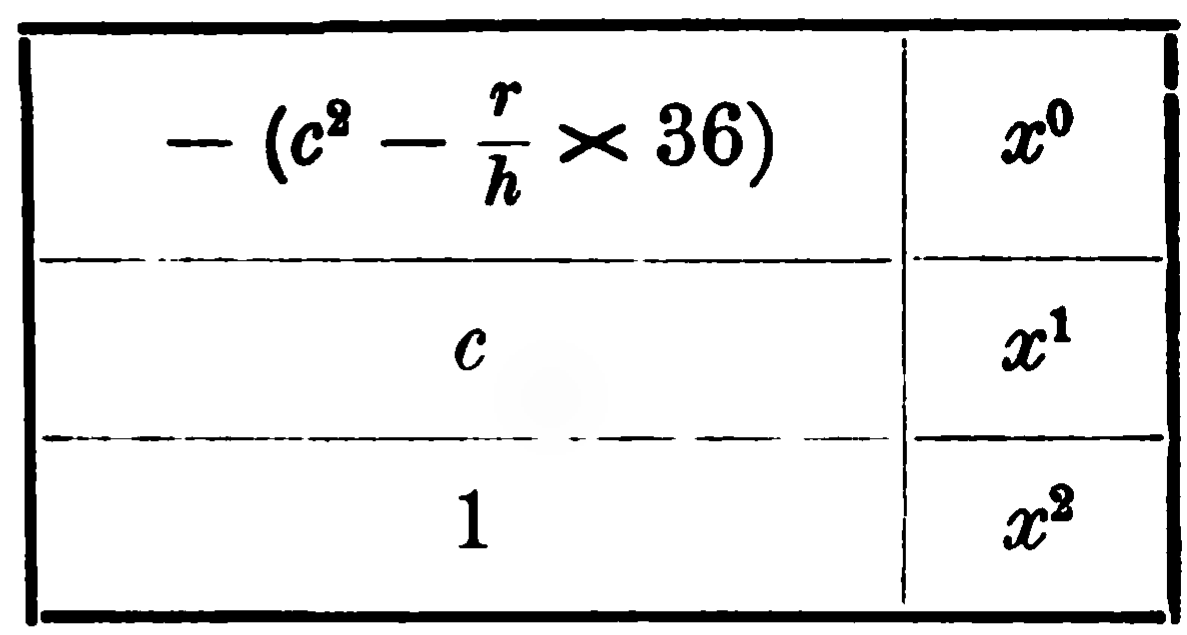
\includegraphics[width=.48\linewidth]{pdf057-quadratic-arrangement.png}\end{center}

A problem in Chang's work, that has become known as the ``problem of hundred hens'' is remarkable, because different suits of solutions are adopted for it. The problem is:

``A cock costs 5 pieces of money, a hen 3 pieces, and 3 chickens 1 piece. If then we buy with 100 pieces 100 of them, what will be their respective numbers?''

This is equivalent to the system of indeterminate equations,
\[
x+y+z=100,\qquad \text{and}\qquad 5x+3y+\frac{1}{3}z=100.
\]

Chang gives the answer to be
\[
\begin{array}{rcl}
(1)& 4\ \text{cocks},&18\ \text{hens and }78\ \text{chickens};\\
(2)& 8\ `` ,&11\ ``\quad ``\quad 81\ `` ;\\
(3)&12\ `` ,& 4\ ``\quad ``\quad 84\ `` .
\end{array}
\]

Chang's rule for its solution is very roughly stated thus:

``The cocks every time increase by 4, the hens decrease every time by 7, and the chickens every time increase by 3; and we get the answers.''

Here Tai Chêng adds in his edition of the work that this rule is hardly intelligible, but that even the commentators Chên Luan and Li Ch'un-fêng are not known to have made its explanation clear. Tai also adds a rule for its solution obtained by Shieh Ch'a-wei, who lived some time in the reign of the Sung Dynasty before the 13th century. This solution is also not of a general kind. To obtain a particular solution, he only suggests that the 100 pieces of price should be divided by $3+3+3=9$, in order to derive the number of hens, because a chicken costs $\dfrac{1}{3}$ pieces, so that the cock and hen must be multiplied by 3 and their numbers be added. The remainder then being subtracted from the divisor 9, gives the number of cocks.

A like problem is also seen in Chên Luan's commentary on the \emph{Su-shu Chi-i} written by Hsü Yüeh who belonged to the Han Dynasty.
\scanfooter

\scanpage{0058}{Part I, printed page 44}

Hsü Yüeh is believed to have been a pupil to Liu Hung, a statesman and astronomer of some renown, who lived about the middle of the 2nd century A. D. According to the \emph{San-kuo Chih} or the ``History of the Three Monarchies'', composed in 285, Han Chai, the astronomer, who became a minister of the Kingdom of Wu, and who died in 243, had learned Liu Hung's calendar theory from Hsü Yüeh. These considerations fix the life-time of Hsü at about the year 200. Chên Luan, the commentator, belonged to the 6th century, as we have mentioned above.

The problem Chên solves in the commentaries on Hsü's work runs: ``If a cock costs 5 pieces, a hen 4 pieces and 4 chickens 1 piece, how many cocks, hens and chickens can be bought with 100 pieces so as to make 100 in all?''

Chên gives his answer to be 15 cocks, 1 hen, and 84 chickens.

If the cock costs 4 pieces, the hen 3 pieces, and 3 chickens 1 piece, the answer becomes 8 cocks, 14 hens, and 78 chickens, as Chên solves it.

Hsü Yüeh says in his text, ``Avoid doing the measurement by calculations as much as possible, let it be effected by mental determination.'' Here Chên Luan explains the meaning of the sentence to be that some problems are better answered by a direct consideration than by the calculating pieces. He thus applies a geometrical construction.

``There is a large river, whose breadth is unknown. It is required to measure it, without using the calculating pieces.''

Here the river is supposed to flow from west to east.

For the solution of this problem, Chên Luan erects three rods on the northern side of the river costraight from north to south and each 10 feet apart; and looks at the two banks of the river from the middle rod, through two points in the southern rod, which will be marked accordingly; he then transfers the heights of these marks to the northern rod and looks through them from the middle rod on two points on the ground, the distance between which gives the breadth of the river that was required to be measured.

In measuring the length of a long staff, Chên Luan erects a rod of known length and with its shadow he measures that of the staff.

To know the depth of a deep well, Chên throws therein a stick, 10 feet long for instance, and looks upon it through the ends of another stick which he holds stretching his hand; he then let a man go back with a stick 10 feet long farther and farther until the stick
\scanfooter

\scanpage{0059}{Chapter 6, printed page 45; end of chapter}

can be seen corresponding to the marks in the stick in his hand; then the distance walked by the man represents the depth of the well.

According to Yüan Yüan\footnote{Yüan's \emph{Biographical Notices}, Book 11.}, Chên Luan composed a calendar system in the reign of the emperor Wu-Ti of Chou. He also wrote commentaries on the \emph{Chou-pei}, Chang Ch'iu-chien's ``Arithmetical Classic'', Tun Ch'üan's \emph{San-têng-shu}, the ``Arithmetical Classic'' of Hsia-hou Yang, the ``Arithmetic in Nine Sections'', the \emph{Wu-t'sao Suan-ching}, and other calendrical works. Chên Luan was a learned man not only in mathematical and allied subjects but he was also profoundly read in books of the Buddhistic religion. He wrote the \emph{Wu-ching Suan-shu} or the ``Arithmetic in the Five Classics'', in which he embodied various problems alluded to in the sacred books, \emph{Yi-ching}, \emph{Shu-ching}, \emph{Shi-ching}, \emph{Lun-i}, etc. A commentary was written on it by Li Ch'un-fêng in the 7th century.

In concluding this chapter, we must own that the treatises we have described in this and preceding chapters are the whole that now remain of the Chinese productions from the oldest times down to the 6th century. There had existed various others that are now all lost. The existant works were certainly only a few among a multitude of those that have been lost. Nor could they be looked upon by any means as the best representatives of the highest mathematical attainments of the Chinese arrived at in those days. But unfortunately we have no means of making any guess at the true nature of the actual state of mathematical studies carried on by the ancient Chinese, except through the few remnants that are nowadays possessed by us. Among the lost we may mention the \emph{Hsü Shang Suan-shu} or the ``Arithmetic of Hsü Shang'', that consisted of 26 books, and the \emph{Tu Chung Suan-shu} or the ``Arithmetic of Tu Chung'', that consisted of 16 books. These two mathematicians Hsü and Tu belong to the age of the Former Han Dynasty, and so are not subsequent to the 1st Christian century. Another instance of a lost work is the \emph{San-têng-shu} of Tun Ch'üan, who seems to have been a contemporary of the astronomer Ho Ch'êng-t'ien, wose life-time lay in the first half of the 5th century.

Of Tsu Ch'ung-chih's \emph{Chui-shu}, which is also lost, we shall speak again in the next chapter.
\scanfooter


\scanpage{0060}{Chapter 7, printed page 46}
\setcounter{footnote}{0}
\begin{center}
CHAPTER 7.\\
THE CIRCLE-MEASUREMENTS BY OLDER\\
CHINESE MATHEMATICIANS.
\end{center}
\phantomsection\addcontentsline{toc}{subsection}{Chapter 7. The Circle-Measurements by Older Chinese Mathematicians}

As we have already observed, the ancient Chinese employed for $\pi$ the value 3, or they counted the circumference of a circle compared with its diameter as 3 to 1. This value of $\pi$ was used in China as early at least as the time of Chou-Kong in the 12th century B. C., and ever subsequently. So was it employed in the \emph{Chou-pei}. The ``Arithmetic in Nine Sections'', on such a high plane in its mathematical attainments as we have described, took no other value of $\pi$. With Sun-Tsŭ, the \emph{Wu-t'sao Suan-ching}, Hsia-hou Yang, Chang Ch'iu-chien and Chên Luan, it was all the same.

But the Chinese did not in any way remain always satisfied only with this rough value of $\pi$. An attempt at circle-measurement appeared soon in the course of progress of mathematical studies.

According to the \emph{Sui-shu} or the ``Records of the Sui Dynasty'', in the section on the ``Calendrical and Allied Subjects'', there had appeared in China a host of circle-squarers in the persons of Liu Hsing, Chang Hêng, Liu Hui, Wang Fan, P'i Yen-tsung and others, who all calculated the length of the circular circumference, who however all obtained results differing in values from one another.

It will not be altogether without interest to give a brief description of the lives of these scholars, though we know little or nothing about the values got by some of them.

Liu Hsing was a younger son to Liu Hsiao, the philosopher, who was of the imperial house of the Han Dynasty. Liu Hsing himself was also a philosopher and was learned in calendrical subjects. The ``San-t'ung Calendar'' was his composition. He held a high office under the usurper Wang Mang.\footnote{Yüan's \emph{Biographical Notices}, Book 2.} He belongs to the first quarter of the 1st century A. D. Unfortunately we are not imformed of his value of $\pi$.

Chang Hêng was a native of Nan-yang. Being intelligent from his very childhood, he had betaken himself mostly to studies on astronomy, calendar-theories, and philosophy or rather fortune-telling. On account of his uncommon erudition he was given an office in the court by the emporor An-Ti. He held for a time the place of chief astrologer, and he served as a minister, before he died, which happened in 139 A. D. He was 61 years old when he died. Chang Hêng constructed a celestial globe that serves to illustrate the motions of
\scanfooter

\scanpage{0061}{Chapter 7, printed page 47}
\setcounter{footnote}{0}
heavenly bodies, making the earth the centre of the system. He also constructed a certain instrument, which is believed to have been a contrivance serving for a seismometer. Chang wrote the \emph{Ling-hsien}, an astronomical work in which he gives a creation-theory of the universe and explains how the world has arisen from chaos or nothing.\footnote{The \emph{Hou-Han Shu}, or ``Records of the Later Han Dynasty''.} Chang's calculation of the circle has been however lost, although his value of $\pi$ is given in a commentary on the ``Arithmetic in Nine Sections'' in the form that the square of the circular circumference and the perimeter of the circumscribed square are as 5 to 8. This is equivalent to take $\pi$ at $\sqrt{10}$.

T'sai Yung, who lived about the years 190---193 A. D., is said to have used the value $\pi=3$, the same as most other ancient mathematicians.

Wang Fan was a general of the Wu Kingdom in South China in the age of the Three Monarchies. When Sun Hao the king or emperor of Wu had held a council of state in the year 267, Wang appeared drunk before his emperor, who became so furiously offended with his rude behabior that he at once drew his sword and cut him down on the spot. Wang was 38 years of age when he died.\footnote{The \emph{San-kuo Chih} or ``Records of the Three Monarchies'', section on biographies.} According to Yüan Yüan,\footnote{Yüan's ``Biographical Collections'', Book 5.} Wang Fan calculated the circle, arriving at the result that if the circumference be 142, then the diameter should be 45. This value corresponds to $\pi=3\cdot1555\ldots$. As to Wang's way of quadrature, however, we have no means of knowing the details. As we learn from the Records of the Chin and Sung Dynasties, Wang had been an able astronomer.

Contemporary with Wang Fan but belonging to a different Kingdom of Wei in North China, there lived another mathematician Liu Hui, about whose life we know nothing except that he wrote in 263 his commentaries on the ``Arithmetic in Nine Sections''. But his commentaries still remain and we find among them the particulars of his quadrature of the circle.\footnote{Commentaries on the ``Nine Sections''.}

Liu Hui starts, in his measurement of the circle, with a hexagon inscribed in a circle whose diameter is taken as 2 feet. Each side of the hexagon is equal to half the circular diameter. On this hexagon Liu Hui describes a dodecagon by doubling the number of its sides,
\scanfooter

\scanpage{0062}{Chapter 7, printed page 48}
then doubles again the sides and describes a 24-gon, and so on. By this way the areas of the polygons thus formed gradually approach to that of the circle, the difference diminishing step by step. ``Hence'', he says, ``doubling and doubling the number of sides, and if we proceed until we can no more continue the process of doubling, the perimeter ultimately comes to coincide with the circumference of the circle, so that by taking its area for that of the circle, no portion however small will go neglected. Therefore multiplying with half circumference to half diameter, we get the circular area.''

To carry out this calculation in actuality, Liu Hui first tries the evaluation of a side of the inscribed dodecagon.

The diameter of the circle being 2 feet, its half or 1 foot is one side of the hexagon. Hence with the radius 1 foot as hypotenuse and with half a side $=0\cdot5$ feet as the second side of a right triangle, we calculate the third side, which is equal to $\sqrt{0\cdot75}=0\cdot866\,025\frac{2}{5}$; and subtracting this from the radius we get $0\cdot133\,994\frac{3}{5}$.

Here of course Liu Hui does not take recourse to the decimal fraction, --- a conception that was entirely wanting in the ancient mathematics of China. By Liu Hui the last written quantity is designated in terms of $0\cdot000\,001$ feet as the unit. It may however be safely said, that the conception of a decimal fraction had been nearly arrived at in the times of Liu Hui and of his successors. In what follows the numbers are expressed with this unit.

Taking the last obtained quantity and the half of a side as the two sides of a right-angled triangle, the hypotenuse square will be calculated to be $26\,79491\,93445$, where the fractional part is postponed. Extracting the square root of the number, a side of the dodecagon is obtained.

Next to calculate a side of the 24-gon, Liu Hui first deduces from a quarter of one side square of the dodecagon and the circular radius the third side of the right triangle with these sides to be $=965\,925\frac{4}{5}$, the difference of which with the radius is $34\,074\frac{1}{5}$.

The square of the hypotenuse of the right triangle with this length and half a side of the 12-gon as two sides is $=6\,81483\,49446$, where the fractional continuation is postponed. This gives the square of a side of the 24-gon.

In like manner, after calculating the two lengths, $991\,444\frac{4}{5}$ and $8595\frac{1}{5}$, Liu Hui gives the square of a side of the 48-gon
\scanfooter

\scanpage{0063}{Chapter 7, printed page 49}
\setcounter{footnote}{0}
$=1\,71102\,78813$, and hence its one side is $=130\,806$. Multiplying it by 1 foot of the radius and also by 24, we have $313\,93440\,00000$.

If we divide this number by a hundred thousands millions, we obtain the area of the 96-gon to be $313\frac{584}{625}$, where the unit of length is taken to be a tenth of one foot.

Again to carry out this calculation for the 192-gon, two quantities $9\,97858\frac{9}{10}$ and $2141\frac{1}{10}$ being derived in similar way as done in the above, the square of one side of the 96-gon is calculated to be $42821\,54012$, $\therefore$ one side $=65\,438$. Multiplying it by the radius and also by 48, we get $314\,10\,240\,00\,000$, or taking its a-hundred thousands millionth part, the area of the 192-gon is found to be $314\frac{64}{625}$ with the same unit as before.

Twice the difference of this area and that of the 96-gon, which is equal to $\frac{210}{625}$, is the sum of the areas of the 96 figures obtained on the outside of the 96-gon by multiplying its sides by their sagittae. If we add this sum to the area of the 96-gon, the result is greater than the circular area. Hence, of the area of the 192-gon Liu Hui takes the integral part only as the determinate value of the circular area, neglecting the fractional part.

When this value is divided by the radius, which is 1 foot, and the result is doubled, we obtain the length of the circumference to be $=6\cdot28$ feet.

Liu Hui compares this length with the diameter, 2 feet, and obtains as the ratio of the circumference to the diameter:
\[
(\text{circumference})=157\quad\text{and}\quad(\text{diameter})=50.
\]

Here Liu Hui adds that in this ratio the moment or modulus of the circumference is taken somewhat smaller than its real value.

Of P'i Yen-tsung's value of $\pi$ we have never met with any mention; nor know we exactly of his date. It seems, however, he was a contemporary of the astronomer, Ho Ch'êng-t'ien, and flourished therefore somewhere about the first half of the 5th century, if we may rely on a slight indication in the \emph{T'ang-shu} or the ``Records of the T'ang Dynasty.''

Men, who lived during the Chin Dynasty, is said to have used the value $\pi=3\cdot14$, and Wu, of Sung Dynasty, the value $\pi=3\cdot1432+$.\footnote{Muramatsu's \emph{Sanso} of 1663, Book 4.}
\scanfooter

\scanpage{0064}{Chapter 7, printed page 50}
Two centuries after Liu Hui, there appeared another and more distinguished circle-squarer, --- I mean Tsu Ch'ung-chih of the Liu-Sung Dynasty. According to the \emph{Sui-shu} or the ``Records of the Sui Dynasty'', the section on calendrical and allied subjects, Tsu contrived a more effective method of proceeding than his predecessors had followed. He took a circle of diameter $1000\,00\,000$ or $10^8$ as equal to 10 feet and obtained for the length of its circumference the upper and lower limits, $3\cdot1415927$ and $3\cdot1415926$, where we have taken the unit to be 10 feet. From these numbers he inferred that the true value of the length must lie between the two, and thereupon he deduced by some way the two fractional values for $\pi$, which were called the accurate and inaccurate values. These were $\frac{355}{113}$ and $\frac{22}{7}$.

The inaccurate value of $\pi$ that Tsu Ch'ung-chih obtained is nothing but the same as arrived at by the Greek Archimedes hundreds of years previously, but as to the other no single page of mathematical history can assure us of its preexistence in any part of the world. As matter of course did the Greeks not possess it. Nor knew the Hindoos anything of it. Even in subsequent years the learned Arabians could not rediscover Tsu's value again. In modern Europe too it was not known until the Dutch mathematician Adriaan Anthoniszoon, father of Adriaan Metius, obtained it first in 1585. The Chinese had therefore been possessed of this, the most extraordinary of all fractional values, over a whole millenium earlier than Europe. We are on this account strongly urged to express a desire that it should henceforth be called by the name of Tsu Ch'ung-chih's fractional value for $\pi$.

Tsu Ch'ung-chih wrote the \emph{Chui-shu} consisting of many books or chapters, in which his calculation of the above value of $\pi$ had been laid down. As we are informed, this book was afterwards adopted by the T'ang government in its mighty system of elective examinations. But it does not exist now; it has been lost. Nevertheless the account we have mentioned above has been preserved fortunately enough, given by Wei Chih in his \emph{Sui-shu} or the ``Records of the Sui Dynasty''. Wei Ch'ih was a learned doctor and able statesman flourishing in the reign of Tai-tsung, the second of the T'ang emperors. He died in the year 643.

Some scholars believe that the term \emph{chui-shu} had meant the method or process, which Tsu used in his illustrious circle-measurement. Thus later scholars both in China and in Japan actually applied this term to the analytical process of measuring the circle, as we shall see later
\scanfooter

\scanpage{0065}{Chapter 7, printed page 51}
\setcounter{footnote}{0}
on. But in my opinion, the term \emph{chui-shu} had originally meant no such process, but was merely a technical term used in the calendrical science or art. So we find the term applied as the motto to some problems of calendrical computations in the \emph{Su-shu Chiu-chang} (1247) of Ch'in Chiu-shao of Sung. Ch'ên Huo of Sung and others used the term also in the same meaning. Some of later Chinese mathematicians have been of the same opinion as we. Therefore we take Tsu's \emph{Chui-shu} as a treatise of calendrical theory, to which his calculation of the circle was appended. Tsu was a great astronomer.

As Tsu Ch'ung-chih had employed the terms \emph{k'ai-ch'a-mi} and \emph{k'ai-ch'a-li}, as is recorded in the ``Records of the Sui Dynasty'', although their meanings are hardly to be discovered and so we are little able to give them corresponding English words, yet some scholars agree in believing in Tsu's resorting to some kind or other of expansion in series, because the obscure terms used by him seem to tell that they were intended to mean the second and third terms in a series. He may have applied a process something like the indeterminate multipliers to determine three terms in an expansion. When we reflect on the uncommon birth of Tsu's genius, we think he might well have done what posterity has wanted to ascribe to him.

According to Wei Chih\footnote{The Records of the \emph{Sui Dynasty}.} Tsu Ch'ung-chih's processes or theories as laid down in the \emph{Chui-shu} were extraordinarily minute in description and elegant in meaning, in so much that he stood at the head of all mathematicians old and recent. The academical officials were little able to understand the deep significance of his writings, which were accordingly left untouched.

The biographical notices of Tsu Ch'ung-chih are recorded in the Biographical Sections of the \emph{Nan-Shih} or ``Records of the Southern Monarchies'' and of the \emph{Nan Chai Shu} or the ``Records of the Chai Dynasty in the South''. These two works hardly differ in their accounts of the life of our great mathematician and astronomer.

Tsu Ch'ung-chih was born in 430 in Fang-yang. He served the Emperor Hsiao-wu of the Monarchy of Sung or of Liu-Sung as it is better known. He lived in a time when power was in a foreign conquerors' hands, and he served in a monarchy founded by the Hun tribes; he himself was however certainly a native Chinese, for his ancestors had been officials of an older native dynasty.

During the reign of Hsiao-wu, Tsu composed a new calendar system of his own. It was just on the eve of being adopted for
\scanfooter

\scanpage{0066}{Chapter 7, printed page 52}
public use in place of the system of Ho Ch'êng-t'ien (died at the end of the Yüan-chia Era covering 424---453), when the emperor died (464) and consequently Tsu's calendar remained unapplied.

Tsu Ch'ung-chih invented a new kind of ``south-pointing vehicle'', which was found to be better than any other of the kind.

Tsu's invention is extraordinarily remarkable, for the two ``Records'' mentioned above equally say that it was moved neither by wind nor by water, but by a special contrivance arranged within itself. He also constructed an automobile vessel, which was neither provided with sails nor rowed by human hands, but that went more than a hundred Chinese miles in a day. The particulars, however, of these contrivances are now all forgotten.

Tsu was not only learned in mathematical sciences, but he was also versed in philosophy. He is said to have composed commentaries on the \emph{Nine Sections} as well as on various philosophical classics.

Tsu Ch'ung-chih died in 501 at the advanced age of 71. In the decline of his life he belonged to the Monarchy of Chai, the Liu-Sung Kingdom having been overthrown in 479. But his work \emph{Chui-shu} is always referred to as written by Tsu Ch'ung-chih of Liu-Sung, indicating that his writing of the treatise happened in the reign of the Sung Monarchy. The Sui Records fixes the date of Tsu's circle-measurement as having been done at the end of the Sung Dynasty and therefore not later than the year 479, twenty years before his death.

Tsu Ch'ung-chih's son Tsu Hong-chih and his grandson Tsu Hao were also both versed in calendrical matters. The latter once held the office of a local Governer General. He was captured and killed in a battle.

Tsu Ch'ung-chih had calculated his accurate and inaccurate values of $\pi$ in the 5th century, but these values were not destined to be soon followed by all his successors. For as we have observed, the mathematicians of the next century, like Chên Luan, Hsia-hou Yang and Chang Ch'iu-chien, used neither of these values. Even the illustrious commentator Li Ch'un-fêng, who flourished in the first half of the 7th century, employed only the inaccurate value given by Tsu, making no mention of the accurate value. Moreover Li referred to Tsu's inaccurate value as the accurate value. Afterwards it was long used by this name. Li may not have known of Tsu's accurate value, but it must be noted that Wei Chih who made a record of Tsu's
\scanfooter

\scanpage{0067}{Chapter 8, printed page 53}
invention of his two fractional values in his \emph{Sui Records}, was a contemporary of Li Ch'un-fêng. Tsu's accurate fractional value was taken up again by Chang Yu-chin many centuries later in the age of the Mongolian yoke.

\begin{center}
CHAPTER 8.\\
WANG HS'IAO-T'UNG AND CUBIC EQUATIONS.
\end{center}
\phantomsection\addcontentsline{toc}{subsection}{Chapter 8. Wang Hs'iao-T'ung and Cubic Equations}

As we have said before, the ``Arithmetic in Nine Sections'' contains a problem whose solution is given by a statement which is equivalent to the general formula for the root of a literal quadratic equation. In another problem in the same work the solution is equivalent to a treatment of the quadratic equation with numerical coefficients. This latter case was also applied by Chang Ch'iu-chien in his Arithmetical Classic. Thus the Chinese had been acquainted with the quadratic equations from so early a date at least at the 2nd or 1st century B. C., and these were being used in the 6th century A. D.

Besides, the ``Nine Sections'' treated of systems of simultaneous equations, and Liu Hui considered in the 3rd century those problems of so complicated a nature that we have mentioned above. All this points out that algebraical manipulations were by no means foreign to the Chinese mathematicians in old times.

Being prepared in this way, then, it is no wonder that we should find a way soon developed in the next age for the solution of cubic numerical equations.

The equations of the third degree come for the first time in the Chinese history of mathematics with the \emph{Ch'i-ku Suan-ching} written by Wang Hs'iao-t'ung at the beginning of the T'ang Dynasty, or in the first half of the 7th century. Of Wang's life we know little or almost nothing, save that he was ordered in his capacity as a Doctor of Arithmetic in the years 623, 626, etc., to carry on an examination upon the contents of the calendar composed by Fu Jên-chün in 618, and that he served as an expert in the Astronomical Board of the T'ang government. But fortunately his work, the \emph{Ch'i-ku Suan-ching}, has remained preserved to this very day, though the last parts are now wanting.

When Wang Hs'iao-t'ung had completed the writing of his work, he presented it to the emperor then on the throne, as we know from his own letter of presentation which remains prefixed to his work.
\scanfooter

\scanpage{0068}{Chapter 8, printed page 54}
But the date of neither his composition nor his presentation is indicated. Nor is it known to which emperor it had been presented. Wang's letter of presentation, however, reveals that the methods employed in the solution of his problems were his own contrivances. The book contains 20 problems, some of which are reproduced in the following lines.

``There is a right triangle, the product of whose two sides is $706\frac{1}{50}$, and whose hypotenuse is greater than the first side by $30\frac{9}{60}$. It is required to know the lengths of the three sides.''

Wang gives the answer of this problem to be $14\frac{7}{20}$, $49\frac{1}{5}$ and $51\frac{1}{4}$. He then proceeds to give the rule:

``The product ($P$) being squared and being divided by twice the surplus ($S$), make the result the \emph{shih} or the constant class. Halve the surplus, and make it the \emph{lien-fa} or the second degree class. And carry out the operation of evolution according to the extraction of cube root. The result gives the first side. Adding the surplus to it, one gets the hypotenuse. Divide the product with the first side and the quotient is the second side.''

The rule is the same as to construct the cubic equation
\[
x^3+\frac{S}{2}x^2-\frac{P^2}{2S}=0,
\]
or the arrangement as annexed, and to solve it in a process similar to the extraction of a cube root. It is very evident that the way of solving an equation of the third degree in this way applies only to numerical equations.

\begin{center}
\renewcommand{\arraystretch}{1.45}
\begin{tabular}{|c|c|}\hline
$-\dfrac{P^2}{2S}$ & $0^0$\\\hline
$0$ & $1^0$\\\hline
$\dfrac{S}{2}$ & $2^0$\\\hline
$1$ & $3^0$\\\hline
\end{tabular}
\end{center}

``In a right triangle, the product of the first side and the hypotenuse is $1337\frac{1}{20}$, and the difference of the hypotenuse and the second side is $\frac{1}{10}$; what is the length of this second side?

``Answer. $92\frac{2}{5}$.

``Rule. The (given) product ($P$) being squared and divided by twice the (given) difference ($D$), we call the result the `solid volume'. Again cube the (given) difference, and halve it, when the difference of this quantity and the `solid volume' should be taken for the \emph{shih} or the constant class. Again square the (given) difference and take its twice as the \emph{fang-fa} or the 1st degree class. Again take $\frac{5}{2}$ of the
\scanfooter

\scanpage{0069}{Chapter 8, printed page 55}
(given) difference as the \emph{lien-fa} or the 2nd degree class. Then (making 1 the 3rd degree class) divide according to the rule of the cubic root extraction. The root gives the length required.''

This rule is equivalent to the construction of the cubic equation,
\[
x^3+\frac{5}{2}Dx^2+2D^2x=\frac{P^2}{2D}-\frac{D^3}{2}.
\]

``In a store-house shaped like a truncated square pyramid, the difference of whose upper and lower sides is 6 feet ($D$) and whose height is 9 feet ($G$) greater than the upper side, there is contained $187\cdot2$ measures of corn, of which $50\cdot4$ measures are carried out. What will be the lengths of the upper and lower sides of the store-house, its height, and the depth and a side of the upper end of the remaining corn?

``Answer. Upper side is 3 feet; lower side is 9 feet; height 12 feet; depth and upper side of the remainder are each 6 feet.''

To find the upper side of the store-house in this problem, Wang Hs'iao-t'ung applies the equation,
\[
x^3+(D+G)x^2+\left(DG+\frac{D^2}{3}\right)x=P-\frac{D^2G}{3},
\]
where $P$ represents the volume of the store-house expressed in cubic feet. This is the very equation to which we are led by eliminating $y$ and $z$ from
\[
y-x=D,\qquad z-x=G,\qquad \frac{1}{3}z(xy+x^2+y^2)=P,
\]
where $y$ and $z$ represent the lower side and the height respectively, and the last equation is in accordance with the formula that appears in the ``Arithmetic in Nine Sections''.

The depth of the remaining corn is obtained from the equation
\[
x^3+3\frac{hs}{D}x^2+3\left(\frac{hs}{D}\right)^2x=\frac{P'}{3}\times\frac{h^2}{D^2},
\]
where $h$ and $s$ denote the height and the upper side of the store-house, and where $P'$ is the quantity of corn carried out measured in cubic feet.

Wang Hs'iao-t'ung gives in the \emph{Ch'i-ku Suan-ching} only his rules for the arrangement of the equations; he does not give the particulars of the procedure for arriving at such equations.

No instance is to be found in Wang's work of equations of the fourth and higher degrees.
\scanfooter

\scanpage{0070}{Chapter 8 ending and Chapter 9 opening, printed page 56}
The treatment of higher equations, together with the algebraical explanation of their construction, appear for the first time in the history of the Chinese mathematics six whole centuries subsequent to the age in which Wang lived.

\begin{center}
CHAPTER 9.\\
ON THE INDIAN INFLUENCE.
\end{center}
\phantomsection\addcontentsline{toc}{subsection}{Chapter 9. On the Indian Influence}

It was in the year 65 A. D., when the Han Emperor Ming-Ti dreaming of a ``golden man'' had sent a messenger to India, that the Buddhist religion was brought to China. Even before that time intercourse may have existed between the two nations, for it is stated in history that the Shamans, Shih-li-fang and others, who made their appearance in China in B. C. 218, were suspiciously sent away by the emperor Shih Hoan-Ti of Ch'in. During Ming-Ti's reign there came Indian Buddhists, Kashiapmadanga, Godharma and others, who settled in China and translated Buddhistic sûtras, the first of a long and tremendous series that followed during the succeeding centuries. Buddhism soon spread over the whole nation, and there arose a great rivalry with the preexisting native religion of the Taoists, out of which the former came victorious.

At first the Chinese translations of Sanscrit works were all done by the Indians or the persons come to China from those countries located in Central Asia. But at length native Buddhists themselves were seen engaged in the matter.

A Chinese Buddhist Fa-hsien visited India from the land through Central Asia and he returned to China in 414 from the sea. He brought with him many sûtras, in the translation of which the remainder of his life was employed.

As will be seen from the account of Fa-hsien's travels and from the fact that the Indian Bôdhidharma came to China in 520 by sea, we know there had existed between China and India a high way over the seas. In these navigations comparatively large boats had been in use, for the sailing vessel that carried Fa-hsien home from India had 200 souls on board, including the crew and passengers.

Hsüan-tsang went to India in 629 and returned to China in 645. On his return Hsüan-tsang occupied his life in the translation of the numerous books he had brought back with him.

In the period of the Southern and Northern Monarchies, that lasted through the 5th and 6th centuries, when China was under the
\scanfooter

\scanpage{0071}{Chapter 9, printed page 57}
yoke of foreign tribes, Buddhism had become universal throughout the whole of the empire, and as we read in history, the Indian works were read in translations ten times more than the native classics, a fact that vividly tells how the Indian influence had swept over the country. Things Indian exercised supremacy in art and literature, in philosophy, in the mode of life and the thoughts of the inhabitants, in every thing. It is even said, astronomy and calendrical arts had also felt their influence. How then could arithmetic remain alone unaffected? Nodoubt the Chinese studied the arithmetical works of the Hindoos.

In the older mathematical works such as the \emph{Chou-pei} and the ``Nine Sections'' we find the value of $\pi$ given merely as equal to 3; we don't find there any other values mentioned; nor see we their authors engaged in the problem of the circle-measurement, of which, it appears, they had taken little care. But the question did not long remain untouched by the Chinese, and yet, as we see, these studies were taken up only after they had come in contact with the Indian civilization; for the Chinese circle-squarers Chang Hêng, Liu Hui, Wang Fan, and others belong all, with the single exception of Liu Hsing who flourished in the first part of the 1st century A. D., to the 2nd and subsequent centuries. Moreover, Wang Fan is said to have embraced the Buddhistic faith, and it was the same with the astronomer Han Chai who served the same monarchy as Wang a short time previous to him. Will it be too rash for us to assume that the problem of the circle-measurement had been transplanted from Indian soil to the fertile land of the Middle Empire?

Of Liu Hui's quadrature of the circle we have already mentioned. The particulars of the calculations as he records in his note to the ``Arithmetic in Nine Sections'' as well as his value there obtained were in all probability owing to himself; yet the first stimulus to his undertaking of such a troublesome attempt might have been, may it not be, got by him directly or indirectly from a Hindoo source or a Central Asiatic? Might not the fundamental principles that have led to Liu's result be borrowed from somewhere outside of the empire?

The same may be the case also with Tsu Ch'ung-chih, although we can never suspect that his extraordinary result could have been derived from without.

Chên Luan to whom we have referred so often was an ardent believer in the Buddhistic faith. He did much in defending the religion against the rivalry of Taoism. Hsü Yüeh's \emph{Su-shu Chi-i}
\scanfooter

\scanpage{0072}{Chapter 9, printed page 58}
applies to a Sanscrit term, and Chên Luan who wrote a commentary on this work of Hsü's refers expressly to Buddhistic sûtras in Chinese translation, although he tells nothing of Indian mathematics. The problems we have described as given by Chên in his note, may perchance be a reproduction from Hindoo works. As to questions in indeterminate analysis we meet with instances only in works that were compiled after the introduction of Buddhism.

But all this, it must be confessed, remains our mere conjecture; there is nothing positive that serves as an evidence of any actual Indian influence upon the Chinese mathematics.

In astronomy some of the Hindoo theories were studied and there are still extant some part of them in translations and quotations. But neither a single problem nor a single rule for solution in the domain of mathematics now remains that is definitely known as of Indian origin.

The fact however that the Indian mathematical works had been studied in China can by no means be denied; for in Wei Chih's ``Records of the Sui Dynasty'', the section on the classical and other works, it is stated that there had been works in Chinese translations like the \emph{Brahman T'ien-wen-ching} or the ``Brahman Astronomical Classic'', consisting of one book, the \emph{Brahman Chieh-ch'ieh Hsien-jên T'ien-wen-shuo} or the ``Astronomical Theories of the Brahman Chieh-ch'ieh Hsien-jên'', consisting of 30 books, the \emph{Brahman T'ien-ching} or the ``Brahman Heavenly-Theory'' consisting of one book, the \emph{Mo-têng-chieh-ching Huang-t'u} or the ``Map of Heavens in the Mo-têng-chieh Sûtra'', consisting of one volume, the \emph{Brahman Suan-fa} or the ``Brahman Arithmetical Rules'' consisting of one book, and the \emph{Brahman Suan-ching} or the ``Brahman Arithmetical Classic'', consisting of three books. These translations are now all lost. We therefore can not know what kind of arithmetical problems or what mode of analysis these works had taught. There had existed nodoubt various other translations of similar works in China.

From the 7th century and downwards Indian scholars were sometimes employed in the Astronomical Board. There are four astronomers recorded in the \emph{T'ang-shu} or the ``Records of the T'ang Dynasty'' who bear the name of Chü-t'an or Gudon and who were officials in the Astronomical Board. These persons were Chü-t'an Chüan, Chü-t'an Lo, Chü-t'an Ch'ien and Chü-t'an Hsi-ta. These astronomers are not exactly stated in the \emph{T'ang Records} to be Indians; but these names tell us they were. For Buddha or Sakiamni is sometimes represented
\scanfooter

\scanpage{0073}{Chapter 9, printed page 59}
in Chinese works as Chü-t'an, which is read Gautama. And the name of Chü-t'an Hsi-ta was to read Gautama Sidharta in all probability.

Of these Indians Chü-t'an Chüan composed a calendar system in 618 for the first emperor of the T'ang Dynasty. Chü-t'an Lo served as the president of the Astronomical Board; a calendar system called the \emph{Kuang-chai Calendar} was his composition.

Chü-t'an Ch'ien was an official in the Astronomical Board; he lived at the end of the 7th century and at the beginning of the next.

Chü-t'an Hsi-ta or Gautama Sidharta translated the \emph{Chiu-chih Calendar} from the Sanscrit into Chinese by an imperial order. He served the Chinese government as the president of the Astronomical Board. We are not informed what kind of a calendar it was, and the work has been lost. But as we learn from a passage in the \emph{T'ang Records}, in this calendar the heavenly circumference, or the circle plainly to speak, was divided into 360 degrees, each of which contained 60 minutes. In this respect it differed widely from the classical usage of dividing the heavens into as many degrees as a year contains days and of subdividing one degree into centesimal parts. The new calendar differed further in not applying to the calculating pieces but in resorting to a written mode of arithmetic. The technical terms used therein, it is stated, were so peculiar that the Chinese scholars who are ever fond of following conservative tendencies were little able to understand its contents.

The employment of the symbol $\bigcirc$ for zero or for the digit that is wanting was probably derived from this translation of an Indian calendrical treatise, or from some other Indian source. This employment does not however occur until the middle of the 13th century, so far as we are informed.

The written arithmetic brought from India is little known to have been practised in China. But the same mode of multiplication as followed in India was considered nearly a millenium later in the \emph{Suan-fa T'ong-tsung} of Ch'êng Tai-wei, which serves as a warrant of the way being preserved in the land of the Chinese perhaps from the time of the translation of the \emph{Chiu-chih Calendar}.

Chü-t'an Hsi-ta also wrote the \emph{K'ai-yüan Chan-ching} or the ``K'ai-yüan Astrological Treatise'', that consisted of 100 books. K'ai-yüan was the title of the Era when the treatise was composed; it covered the years 713---741. This work is said to be a valuable source of information.
\scanfooter

\scanpage{0074}{Chapter 9, printed page 60}
\setcounter{footnote}{0}
Soon after Chü-t'an Hsi-ta's translation of the \emph{Chiu-chih Calendar} there appeared the native Buddhist priest I-hsing, who loved seclusion and cared nothing for distinction, but who was urged to serve the emperor as his adviser, in which capacity he proved an able and distinguished character. As he was deeply learned in astronomy he was ordered in 721 to compose a calendrical system, which he accomplished in 727. I-hsing's system is known as the \emph{T'ai-yen Calendar}. He contrived an arithmetical method called the \emph{t'ai-yen shu}, by applying which he succeeded in the construction of his system. The \emph{t'ai-yen} method was a consideration in the indeterminate analysis. This was the same that led to the beautiful process of the \emph{t'ai-yen ch'iu-i shu} established six centuries later by Ch'in Chiu-shao at the end of the Sung Dynasty.

I-hsing was born in 683 and he died in 727 at the comparatively early age of 44, when his composition of the \emph{T'ai-yen Calendar} was just complete. His life was full of wonderful miracles; he was one of those experts in magic not rare among learned priests.\footnote{The \emph{Records of the T'ang Dynasty}, Biographical Notices.}

After I-hsing was dead and his calendar-system had been ordained for practice, the learned Indian Chü-t'an Ch'ien, who was dissatisfied in not being employed in the late calendrical composition, made an accusation with the astronomer Ch'ên Yüan-ching in 733 that I-hsing's calendar was nothing but copied from the \emph{Chiu-chih Calendar} and that in copying he was even left behind by the original. Nan-kung Shuo too disapproved it. Hereupon were made observational verifications of various calendars in the Imperial Observatory, when I-hsing's calendar was found to stand the actual test for 7 to 8 times in 10, while the calendar composed by Li Ch'ung-fêng proved good 3 or 4, and the \emph{Chiu-chih} only 1 or 2. Consequently the accusers were silenced and condemned. As the ``Records of the T'ang Dynasty'' adds here, there had been twenty-three different systems of calendars since the \emph{T'ai-ch'u Calendar} down to Li Ch'ung-fêng's. These calendars had gradually become more accurate, but they did not go as yet very exactly with the actual progress of the heavens. On the contrary the system of I-hsing answered very minutely, and it was imitated by the calendar-makers for a long time in the succeeding centuries.

I-hsing was a Buddhist priest and he was an extraordinarily learned man, even versed in Sanscrit. It was therefore no wonder that he should have been suspected of consulting an Indian calendar in his composition. If not entirely imitating the processes in the \emph{Chiu-chih}
\scanfooter

\scanpage{0075}{Chapter 9 ending and Chapter 10 opening, printed page 61}
\setcounter{footnote}{0}
\emph{Calendar}, yet he had consulted the contents of the \emph{Chiu-chih Calendar}, as we learn in the ``T'ang Records''.

The possibility of the Chinese mathematic having been influenced by the science of India may well be conjectured from the meagre account here given. As for exact information, we have none.

\begin{center}
CHAPTER 10.\\
CH'ÊN HUO.
\end{center}
\phantomsection\addcontentsline{toc}{subsection}{Chapter 10. Ch'ên Huo}

After I-hsing's time during the long reign of the dynasties of T'ang and Sung, mathematics was undoubtedly cultivated and made some progress; but we have few particulars of these ages. Ch'ên Huo and Shieh Ch'a-wei are the only two men we can mention as belonging to this period, of whom we have some knowledge. We therefore give in this place what we know about these two mathematicians, which, we hope, may serve as a link that connects the age of the older mathematicians we have already described and the flourishing period of the Chinese algebra in the 13th and 14th centuries, when Ch'in Chiu-shao, Li Yeh and Chu Shih-chieh were active.

As to Shieh's life we know nothing except that he wrote an arithmetical treatise known by his name. His note on a problem in Chang Chiu-chien's work we have mentioned already in connection with the latter.

Ch'ên Huo was a native of Ch'ien-t'ang and he was once the president of the Astronomical Board; he then held ministerial rank. He died in 1075 at the age of 64. As astronomer he was able.\footnote{The \emph{Records of the Sung Dynasty}, section on Biographies.}

He wrote the \emph{Mong-hsia Pi-t'an} or the ``Talks Recorded at Mong-hsia'', in which he records two arithmetical contributions of his own. These we explain in this place.\footnote{Ch'ên Huo's \emph{Talks Recorded at Mong-hsia}.}

The volume of a wedge-shaped figure whose head is parallel to the base is obtained as in the ``Arithmetic in Nine Sections'', according to the formula
\[
\frac{1}{6}\{(2a+a')b+(2a'+a)b'\}h,
\]
where $a$ and $b$, $a'$ and $b'$ are the lengths and breadths of the upper and lower bases, and $h$ the height. ``When we have to apply this formula'', says Ch'ên Huo, ``to the calculation of the number of wine-
\scanfooter

\scanpage{0076}{Chapter 10, printed page 62}
kegs in a pile whose form is of a truncated wedge as just considered, the result will be seen not exactly answering to the case. This deviation of the results arises because there are vacancies between the kegs and the two cases are not quite the same. The result is to be somewhat smaller in number. If however we add to the above formula the quantity $\frac{1}{6}(b'-b)h$, the sum represents the number required.

``If for instance the uppermost layer consists of $2^2$ kegs and the lowest of $12^2$, there are 11 layers, and we find the number of kegs in the pile thus:
\[
\frac{1}{6}\{(2\times2+12)\times2+(2\times12+2)\times12\}\times11
\]
\[
{}+\frac{1}{6}(12-2)\times11=649.''
\]

This was perhaps the first instance of the Chinese trying the summation of a progression.

As Ch'ên Huo says, in measuring the areas of fields the process in old treatises suffices for both rectilinear and circular shapes; but there was no method devised for the determination of a circular arc. He himself was not able to give a thorough process but tried to solve the problem in one way. The following lines are taken from Ch'ên's own words:

``Arrange the diameter of the circular field and halve it; then the result is to be taken as the hypotenuse. Let the difference, that arises when the radius is diminished by the divided part (or the sagitta), be the first side. Subtract the square of this side from that of the hypotenuse; extract the square-root of the remainder, and take the result as the second side. Twice this side is the chord of the segmental field. Square the divided part (or the sagitta) and lower its digits by one position, and double the result. Again, divide the result by the diameter and add the chord, which gives the arc of the divided circular field.''

In this rule, the lowering of digits by one position, which is the same as dividing by 10, is little intelligible. But here Ch'ên Huo himself tries a comment, by dint of which we are able to judge that the rule is meant to express the arc of a circle according to the formula,
\[
(\text{arc})=(\text{chord})+2\times\frac{(\text{sagitta})^2}{(\text{diameter})}.
\]
\scanfooter


\scanpage{0077}{Chapter 10 conclusion and Chapter 11 opening, printed page 63}
\setcounter{footnote}{0}
Yüan Yüan\footnote{Yüan's \emph{Biographical Notices}, Book 20.} refers to this process of Ch'ên as the harbinger of the way that Kuo Shou-ching used two centuries later for the same purpose, involving an equation of the fourth degree.

\begin{center}
CHAPTER 11.\\
CH'IN CHIU-SHAO.
\end{center}
\phantomsection\addcontentsline{toc}{subsection}{Chapter 11. Ch'in Chiu-Shao}

The 13th century in China was an age of bustle and disorder. The formidable Tartar monster Genghis Khan made his appearance at the beginning of the century; he proved a terror not only to the Chinese but generally to the whole of the Asiatic countries. The two rival monarchies of Sung and Chin were both pressed on by the Mongolian conquerors. The Kingdom of Chin was overthrown. The Chinese struggled for life and existence. The savage Mongolians ever pressed on to conquer. China was deprived of territory after territory, until it sunk destroyed in 1279.

The 13th century was such an age. Among the very bustle of attack and defence, under the very agony of life and death, that occupied the times, who could ever expect a sound footing won for the progress of mathematical science? But in actuality such was the case. It was just during this epoch that the highly esteemed scholars Ch'in Chiu-shao and Li Yeh came out from among the contending powers. The solution of higher equations and the explanation of algebraical considerations descend from the hands of these two mathematicians.

Ch'in Chiu-shao wrote in 1247 the \emph{Su-shu Chiu-chang} or the ``Nine Sections of Mathematics'', in which he explained the process of solving numerical equations of all degrees. The beautiful proceeding in the indeterminate analysis known under the name \emph{t'ai-yen ch'iu-yi-shu} that had come down from Sun-Tsŭ's problem and through I-hsing's skilled hands, was also laid down in this treatise. Ch'in's work must not be considered an edition of the \emph{Chiu-chang Suan-shu} or the ``Arithmetic in Nine Sections'', because of his adopting the title of \emph{Chiu-chang}. He adopted that title because he considered his subjects as distributed in nine separate sections, which are not the same as the headings in the ``Arithmetic in Nine Sections''.

Of Ch'in's life no authentic history makes any record; but something about his biography is stated in the ``Subsequent Collections''
\scanfooter

\scanpage{0078}{Chapter 11, printed page 64}
\setcounter{footnote}{0}
of the \emph{Kuei-hsin T'sa-chih} written by Chou Mi. According to this book, Ch'in Chiu-shao enlisted in the army at the age of seventeen as a captain of volunteers. He was ingenious from childhood, and was deeply learned in astronomy, music, arithmetic, and in the art of architecture. In poetry too he was no stranger. In all arts of amusement, in riding, in fencing, in shooting arrows, he was a dexterous hand. Endowed with such a brightness of intellect, he was naturally proud, he loved extravagance. Ch'in showed little faith in his friends; his character was of a loose nature.

Of Ch'in's leading a military life, he himself writes in the preface to the \emph{Su-shu Chiu-chang}. He also states about his studying at the Astronomical Board, and learning arithmetic from a certain wise man retired in seclusion. He survived the dangers of stones and arrows, but he was caught with a disease from which he suffered for ten long years, when his heart sinking within him, he found himself an utterly disappointed man. But gaining at length a firm faith in the inevitableness of fate, he recovered his vigorous spirit and was now free once more to employ his hours in studies, the outcome of which was the production of the treatise that should be ever highly esteemed by the students of Chinese mathematics.

The dates of Ch'in's birth as well as of his death are utterly unknown. Nor know we much about the particulars of his life.

According to Yüan Yüan,\footnote{Yüan's \emph{Biographical Notices}, Book 22.} Ch'in served the Sung Government at Chien-k'ang Fu in 1244 and during the Pong-yu Era (1253---1258) he was in his service on the banks of the Yang-tse River. He was made afterwards the governor of Ch'iung Chou and then of Mei Chou, where he died.

Ch'in Chiu-shao's \emph{Su-shu Chiu-chang} was not originally given under this title by its author. Ch'in appears to have called it the \emph{Su-shu} or the \emph{Su-hsiao} merely, as we learn from the statement made by Chang Ch'i-mei\footnote{Chang's preface is dated 1616.} in his copy of the work which he had made from another copy of Wang Ying-lin, the latter being taken again from the manuscripts among the \emph{Yuan-lo T'ai-tien} or the \emph{Yuan-lo Great Collections}. Ch'in's work as we now possess it was printed from Chang's copy. In the \emph{Great Collections}, it was called, however, it seems, by the title of \emph{Su-hsiao Chiu-chang}, which was perhaps Ch'in's original title.
\scanfooter

\scanpage{0079}{Chapter 11, printed page 65}
Ch'in treats 81 problems in his work distributed in nine sections, making eighteen books or chapters. His grouping of problems is done neither according to the old ``Nine Sections'' nor to the different methods of treatment, but merely in accordance with the species of problems considered. Every sort of arithmetical rules found in the ``Nine Sections'' and the ``Sea-island Arithmetic'' are retaken by Ch'in under various heads and often in more complicated forms. Ch'in does not however consider very easy problems in his book.

Ch'in first considers some problems which he solves by means of a method called the \emph{t'ai-yen ch'iu-i-shu}. Ch'in says in his preface that this method was not treated in the ``Arithmetic in Nine Sections'' but that it has been developed in the hands of calendar-makers or astronomers. Here he is certainly alluding to the priest I-hsing and others The method concerns the treatment of some problems in indeterminate analysis.

We have mentioned Sun-Tsŭ's solving a problem in the indeterminate analysis. It was to find a number that gives 2, 3 and 2, respectively, as the remainders, when divided repeatedly by 3, 5 and 7. His rule for the solution however does not indicate in what way it was obtained. Now Ch'in Chiu-shao's process applies to the treatment of this kind of problems. We shall illustrate the process by applying it to Sun-Tsŭ's problem, because it seems to afford a most suitable example for our purpose.

The numbers 3, 5 and 7, that appear in the problem, are called by Ch'in the \emph{yuen-su} or the original numbers, which he arranges in a vertical column. He then arranges unity against each of these original numbers to the left of them. These are called the \emph{t'ien-yuen} or the celestial elements or celestial monads. The term ``celestial element'' is very noteworthy in the history of Chinese mathematics, as we shall see later on. The arrangement is effected as annexed,
\[
\begin{array}{c|c}
1&3\\ \hline
1&5\\ \hline
1&7
\end{array}
\]

The numbers in the left column are cross multiplied by those of the right column, or each celestial element is multiplied by the original numbers not pertaining to it. The results are called the \emph{yen-su} or operation-numbers. The arrangement thus becomes
\[
\begin{array}{c|c|c|l}
3&5&7&\text{original numbers}\\ \hline
35&21&15&\text{operation-numbers.}
\end{array}
\]

Here we have represented the arrangement in horizontal lines for the sake of convenience, though originally vertically arranged.
\scanfooter

\scanpage{0080}{Chapter 11, printed page 66}
If there be a factor common to two or more of the original numbers, this factor should be removed from these numbers, retaining it only in one of them. The original numbers are thus to be made such that every two of them are prime to one another. The numbers thus simplified are called the \emph{ting-mu} or definite base-numbers. The operation-numbers such as obtained in the above are to be formed from the base-numbers.

The definite base-numbers are taken as moduli and the congruences are formed with their respective operation-numbers. Thus we have in our case
\[
35\equiv2\pmod 3,\qquad 21\equiv1\pmod 5,\qquad 15\equiv1\pmod 7.
\]

The residues of these congruences are called the \emph{ch'i-su}. The results are arranged thus
\[
\begin{array}{c|c|c|l}
3&5&7&\text{base-numbers}\\ \hline
2&1&1&\text{residues}
\end{array}
\]

The residues that are unity are at once taken for the multipliers. With residues that are not unity, the corresponding multipliers are to be found according to a method called the \emph{t'ai-yen chiu-i-shu} or the great extension method of finding unity if we have to literally render the term. We shall shortly describe this process in full, but for the present we have to find in particular the multiplier for the base-number 3, whose corresponding residue is 2.

For this purpose the residue 2 is arranged in the right upper space, and the base-number 3 under it. Then the celestial element or unity is put to the left of the residue, thus
\[
\begin{array}{l|l}
1\ (\text{celestial element})&2\ (\text{residue})\\ \cline{2-2}
&3\ (\text{base-number})
\end{array}
\]

The base-number 3 is divided by the residue 2, when we get the integral quotient 1, and the remainder 1. The quotient is multiplied by the celestial element, giving the product 1, which is called the \emph{kuei-su} or reduced number. It is arranged below the celestial element, thus
\[
\begin{array}{l|l}
1\ (\text{celestial element})&2\ (\text{residue})\\ \hline
1\ (\text{reduced number})&1\ (\text{remainder of base})
\end{array}
\]

The next step is to divide the residue 2 by the remainder 1 of the base-number, getting the quotient 1, for in the end of the operation the remainder obtained from the residue in the right upper space
\scanfooter

\scanpage{0081}{Chapter 11, printed page 67}
should be made unity. This quotient is to be multiplied by the number arranged in the left under space, and the result is to be added to the left upper number. The result becomes 2, giving the arrangement
\[
\begin{array}{l|l}
2&1\ (\text{remainder of the residue})\\ \hline
1\ (\text{reduced number})&1\ (\text{remainder of the base})
\end{array}
\]

When thus the remainder of the residue becomes unity, the operation has been brought to an end, and the number obtained now in the left upper space will be taken for the required multiplier.

The multipliers thus obtained are then arranged in the following way:
\[
\begin{array}{c|c|c|l}
3&5&7&\text{base-numbers}\\ \hline
35&21&15&\text{operation-numbers}\\ \hline
2&1&1&\text{multipliers}
\end{array}
\]

The operation-numbers should be multiplied by the corresponding multipliers, when we obtain the \emph{fan-yung} or the reduced use-numbers, which will be arranged in this way:
\[
\begin{array}{c|c|c|l}
3&5&7&\text{base-numbers}\\ \hline
70&21&15&\text{reduced use-numbers}
\end{array}
\]

The continued product of the definite base-numbers is called the \emph{yen-mu} or operation-modulus, which is 105 in our case.

When common factors have been removed, these removed factors should be restored now, the corresponding use-numbers being multiplied by them. In this way the reduced use-numbers become the definite use-numbers.

In our case the reduced use-numbers are themselves the definite use-numbers. These are the same numbers as employed by Sun-Tsŭ in his rule of solution. Multiplying them by the respective remainders given in the problem, their sum is to be repeatedly diminished by the operation-modulus, when we get the desired answer, which is 23.

The above is not Ch'in's own description but we have tried to represent as exactly as possible the actual way of his treatment of the process. This same way is applicable to the general case where a number is to be found such that it will give when repeatedly divided by $m_1,m_2,m_3,\ldots,m_n$ the remainders $r_1,r_2,r_3,\ldots,r_n$. We shall only consider the divisors as having no common factors between any two of them.
\scanfooter

\scanpage{0082}{Chapter 11, printed page 68}
To determine such a number, we have only to find the undetermined multipliers $\varrho_1,\varrho_2,\varrho_3,\ldots,\varrho_n$ in the expression
\[
M=r_1M_1\varrho_1+r_2M_2\varrho_2+r_3M_3\varrho_3+\cdots+r_nM_n\varrho_n,
\]
where for $M_1,M_2,\ldots,M_n$ we understand numbers of the type
\[
M_k=m_1m_2\cdots m_{k-1}m_{k+1}\cdots m_n
=\frac{m_1m_2\cdots m_n}{m_k}.
\]

The quantities $M_2,M_3,\ldots,M_n$ all contain the factor $m_1$, so that the remainder of $M$ when it is divided by $m_1$, is the same as that of the first term for its expression. We have therefore to determine $\varrho_1$ in such a way that $M_1\varrho_1$ becomes $\equiv1$ with the modulus $m_1$. It is obvious that $M_1$ may be replaced by its residue $R_1$ for the modulus $m_1$ for the determination of $\varrho_1$. It is consequently only necessary to find the integral value of $\varrho_1$ satisfying the relation $\varrho_1R_1-pm_1=1$.

If $R_1=1$, it follows at once that $\varrho_1$ is to be taken also $=1$, for $p=0$ establishes the relation. In the contrary case the determination is to be made by the method of finding unity, of which Ch'in gives a general description, that runs as follows:

``Arrange the \emph{ch'i} (or $R_1$) at the right upper space, the \emph{ting} (or $m_1$) at the right under, and the celestial element at the left upper. First divide with the right upper the right under; the (integral) quotient obtained should be multiplied by the number in the left upper and (the product) should be entered into the left under. Then repeat the process with the two members in the right column, dividing the greater by the less. The obtained quotients should be every time cross multiplied by the left upper or under and added to the other. The operation should be brought to an end when the \emph{ch'i} (or the right upper) is reduced to unity. The quantity now obtained in the left under is the multiplier required.''

This rule is the same, $Q_1,Q_2,\ldots,Q_{2k}$ being the successive quotients, as to form the quantities
\[
\begin{aligned}
A_1&=1Q_1, & A_2&=A_1Q_2+1, & A_3&=A_2Q_3+A_1,\\
A_4&=A_3Q_4+A_2, & \ldots\ ,&& A_{2k}&=A_{2k-1}Q_{2k}+A_{2k-2},
\end{aligned}
\]
of which the last is taken for the required value of $\varrho_1$.

Some of the problems considered by Ch'in of the same nature are reproduced in the following:

``In old calendars the winter solstice returns in $365\frac14$ days, the lunar month in $29\frac{499}{940}$ days, and the \emph{kia-tsŭ} (or sexagesimal cycle) in
\scanfooter

\scanpage{0083}{Chapter 11, printed page 69}
60 days.\ .\ .\ . In how many years or months or days will these three return to the same concurrence .\ .\ .?''

``There were three farmers who divided the rice they had raised in common .\ .\ . equally among themselves. They went to different places, where different standards of measure were being used, and sold their shares, as much as could be exactly measured by the respective standards of the places .\ .\ ., when A had $0\cdot32$, B $0\cdot70$, and C $0\cdot30$ measures of rice left in their hands. What would have been the total amount raised by the three and the respective measures sold by them separately?''

In this problem the measures of the three places are taken to be $0\cdot83$, $1\cdot10$, and $1\cdot35$ units of the common standard, with which the total is to be measured.

This problem is solved according to the general scheme we have mentioned above. The respective standards of measure 83, 110, and 135 are taken for the original numbers with which the sum total is to be divided, giving the remainders 32, 70 and 30, respectively.

In chapter or book 4, Ch'in gives a problem that relates to the volume of a circular keg, the diameters of whose mouth, middle section, and base, are $1\cdot05$, $2\cdot4$ and $0\cdot8$ feet ($m,s,b$), respectively, and whose depth is $1\cdot6$ feet ($d$), and that contains water to the depth of $1\cdot2$ feet ($w$). Ch'in gives the solution, without making any explanations whatever, like all other problems in the work, as follows. Here of course he writes in full words. Thus
\[
A=(bs+b^2+s^2)\times\frac d2\times11,\qquad A'=42,
\]
\[
B=\frac d2\times m+\left\{\left(\frac d2+w\right)-d\right\}\times(s-m),
\qquad C=\frac d2\times s,
\]
\[
D=B^2+C^2+BC,\qquad D'=\left(\frac d2\right)^2\times42;
\]
and he gives
\[
(\text{lower half volume})=A\div A',
\]
\[
(\text{diameter of water surface})=B\div\frac d2,
\]
\[
(\text{upper half volume})=D\div D',
\]
and the contained water will be measured in a cylindrical form with the section equal to the mouth of the keg and with the depth
\[
\left\{\left(\frac d2\right)^2\times A+D\right\}\div(m^2\times D').
\]
\scanfooter

\scanpage{0084}{Chapter 11, printed page 70}
In this place Ch'in employs the value of $\pi=\frac{22}{7}$, which he calls the \emph{accurate value}, as Li Ch'un-fêng had done. In another place, however, he employs the old value of 3. And sometimes, so for instance in book 6, he refers to the value $\pi=\sqrt{10}$. Thus in a problem concerning an annular field, he says:

``Take the diameters of the circles in the ring, and square them, and advance the results by one position (which is equivalent to multiplying by 10), when we get the dividends; take unity as the second degree class, and carry out the evolution for the square root; we then get the circumferences.

``Take the circumferences of the circles in the ring, and square them, and retrogress the results by one position (that is, divide by 10), when we get the dividends; take unity as the second degree class and carry out the square-root extraction, when we get the diameters.''

Here Ch'in takes $\pi^2=10$. The same value of $\pi$ was used by Chang Hêng, as we have said. It is curious this same value should have been also employed in India and Arabia. We cannot however conclude that Ch'in might have learned from his Hindoo or Arabian predecessors of this value, because Chang Hêng had lived in an age that precedes the times where the records are made of the Hindoo and Arabian employment of the same value. The same value appears again in the mathematical history of China, and this time quite recently. The earlier Japanese mathematicians too employed it.

In book 5, Ch'in gives the area of a scalene triangle thus:

``With the square of the smallest side add to the square of the greatest side, therefrom subtract the middle side square, and take the half of the remainder, which should be squared in the upper line. With the smallest side square multiply the greatest side square and therefrom subtract the quantity in the above; divide the remainder by 4 and take as the dividend. Take unity as the positive second degree class, and carry out the square-root extraction, when we get the area.''

This rule is the same as expressed by the formula,
\[
\sqrt{\frac14\left\{c^2a^2-\left(\frac{c^2+a^2-b^2}{2}\right)^2\right\}}
=\sqrt{s(s-a)(s-b)(s-c)},
\]
where $a,b,c$ represent the three sides, $a$ and $c$ being the greatest and the smallest, and where $s=\frac12(a+b+c)$.
\scanfooter

\scanpage{0085}{Chapter 11, printed page 71}
In the calculation of the area of a quadrangle, Ch'in does not follow the erroneous views employed in the \emph{Wu-t'sao Suan-ching} and adopted by Hsia-hou Yang. Ch'in calculates the area by the four sides and a perpendicular from a vertex to one of its opposite sides and applies the formula obtained for the triangle.

For the area of a quadrangle with two pairs of equal sides $a$ and $b$ and with the diagonal $c$ that join the ends of these pairs, Ch'in employs the equation
\[
-(B-A)^2+2(A+B)x^2-x^4=0,
\]
where
\[
A=\left\{b^2-\left(\frac c2\right)^2\right\}\times\left(\frac c2\right)^2,
\qquad
B=\left\{a^2-\left(\frac c2\right)^2\right\}\times\left(\frac c2\right)^2.
\]

\begin{center}
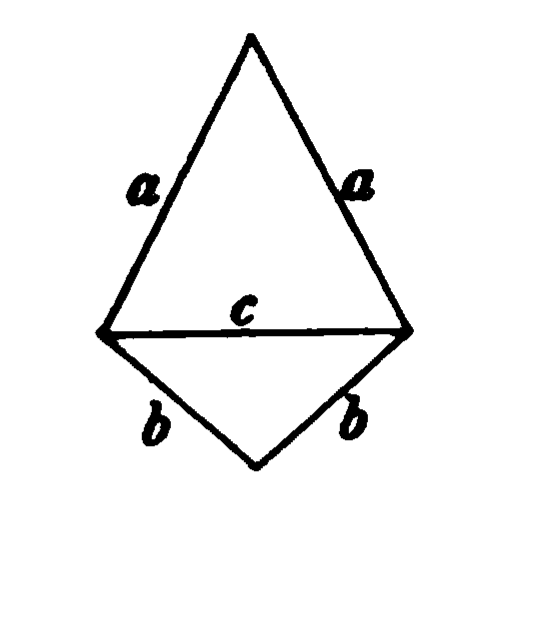
\includegraphics[width=0.18\textwidth]{pdf085-quadrangle.png}
\end{center}

Half the area of a banana-leaf shaped field is given by the equation
\[
-(a+b)^3\times10+\left\{\left(\frac a2\right)^2-\left(\frac b2\right)^2\right\}x+x^2=0.
\]

The field is included by two equal circular arcs, whose common chord is $a$, and whose common sagitta is $b$. This equation is therefore one that gives the area of a circular segment, whose chord is $a$ and whose altitude is $b$.

The book contains a problem on the equal partition of a trapezoid field. This is the earliest instance of various problems of the same nature that attracted much attention among later Chinese and Japanese mathematicians. The problem is this:

``There is a field, whose form is like a rudder; the south side is smaller and measures 34 paces ($a$), the north side is greater and measures 52 paces ($b$); the normal length is 150 paces ($h$). The field is possessed by three brothers, to whom it is to be equally divided. In the division a path is to be provided by a side. It is required to find the respective lengths, etc., of the distributed parts.''

For the length of A's share that comes in the south side, the equation is given:
\[
-\frac K2\times h+ahx+\frac{b-a}{2}x^2=0,
\]
where $K$ is the quotient of $(a+b)h$ divided by the number of persons.

In book 8, Ch'in gives the following problem:

``There is a circular castle, whose circumference and diameter are unknown; it is provided with four gates and three miles ($a$) out of the
\scanfooter

\scanpage{0086}{Chapter 11, printed page 72}
north gate there is a large tree, which is visible from a point 9 miles ($b$) east of the south gate. What will be the lengths of the circumference and the diameter of the castle? Here the old value of $\pi$ is to be used.''

\begin{center}
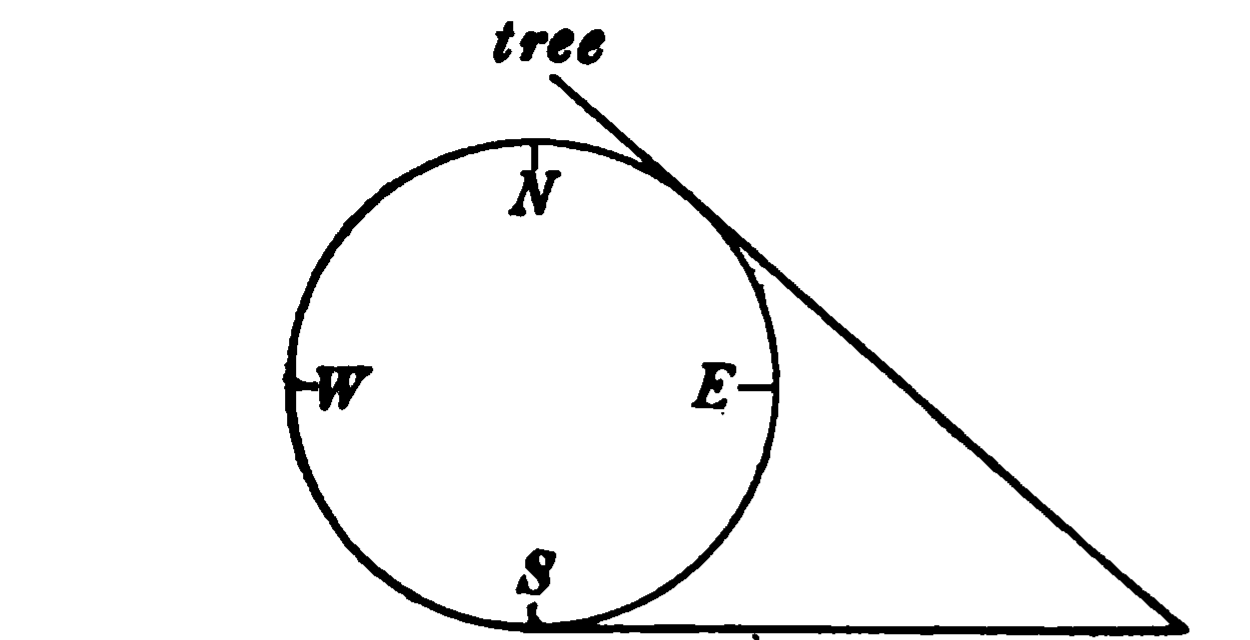
\includegraphics[width=0.45\textwidth]{pdf086-castle-tree.png}
\end{center}

Ch'in solves it according to the equation
\[
1x^{10}+7ax^8+8a^2x^6-4(b^2-a^2)x^2-2b^2\times8a^2x^2-2b^2\times8a^2\times b=0,
\]
which is treated as one of the 10th degree.

This gives the root $x=9$, for the length of the diameter. The treatment of equations of higher degrees appeared with the Chinese mathematicians first in Ch'in's work.

A problem in book 14 is this:

``There is a pile of cedar timbers accumulated in a triangular form. The number in the pile not being known, it is only known that when the timbers are taken away to the middle part, the remaining layer will consist of 9 timbers. The original number and the remaining are required.''

This is a problem of arithmetical progression, and the rule given by Ch'in shows that the sum of such a progression will be expressed as equal to
\[
=\frac{2(\text{the middle layer})\times\{2(\text{middle layer})-1\}}{2}.
\]

In books 15 and 16 there are further some problems concerning arithmetical progressions. He gives as the sum of the first $r$ natural numbers and as that of those from $k$ to $r$ the formulae,
\[
\frac{r(r+1)}2\qquad\text{and}\qquad
\frac{r(r+1)}2-\frac{(k-1)k}{2}.
\]

Ch'in also makes use of the formula
\[
a+(a+b)+\cdots+\bigl(a+\overline{r-1}\,b\bigr)
=\frac b2r^2+\left(a-\frac b2\right)r.
\]

Book 12 contains a problem relating to the number of months that will be required in repaying the sum of 500000 by a monthly payment of 100000, the interest being reckoned at the rate of $0\mathbin{\cdot}65\%$ per month. In solving this problem Ch'in merely calculates the remainders after each payment; he does not use any method of general treatment, although he employs equations of higher degrees in other
\scanfooter

\scanpage{0087}{Chapter 11, printed page 73}
places. He was probably unaware of the general formula that gives the sum of numbers in a geometrical progression.

In book 17 the ancient treatment of the simultaneous linear equations is given in writing in such a form as is annexed. Of course the letters are intended to represent the numbers recorded in numerals representing the forms of the arrangement of calculating pieces. It must not be supposed that Ch'in had recourse to a written mode of manipulation for the simultaneous system. For he only writes down what is to be arranged and carried out on the board for calculating pieces.

\begin{center}
\renewcommand{\arraystretch}{1.25}
\begin{tabular}{|l|c|c|}\hline
weight & $a$ & $a'$ \\ \hline
salt & $b$ & $b'$ \\ \hline
silver & $c$ & $c'$ \\ \hline
\end{tabular}
\end{center}

The numerals Ch'in employs in his work, and indeed very freely throughout in all parts of it, differ little from what we have given as the arrangements of the calculating pieces in connection with our view of Sun-Tsŭ. Besides he used the symbol $\bigcirc$ for zero. Such symbols as \rodglyph{1.45em}{pdf087-rod-numeral-4.png}, \rodglyph{1.45em}{pdf087-rod-numeral-5.png}, \rodglyph{1.45em}{pdf087-rod-numeral-9a.png}, \rodglyph{1.45em}{pdf087-rod-numeral-9b.png} are also employed to indicate 4, 5, and 9, the two last symbols both representing 9. In Ch'in's notation, the principle of local value is strictly observed. But this is no wonder, for it is a mere way of writing down what should be arrranged on the calculating board, where the same principle was followed from time immemorial. The symbol for cipher was certainly borrowed from an Indian source, perhaps through the Chinese translation of the \emph{Chiu-chih-Li}, which is now lost. Although its use first occurs in Ch'in's work in so far as we know, yet Ch'in was not in all probability the first to use this symbol in China.

We have spoken of Ch'in Chiu-shao's resorting to higher equations in solving some of his problems. He also explains in detail the actual steps of solving such equations. We have here to describe the practical process of extracting a root of a numerical equation as carried out by Ch'in.

The Chinese practised abacus arithmetic with the calculating pieces, or the sangis, as we have observed, from ancient times. They extracted the square and cube roots on the sangi-board, and indeed on the same principle in both cases. They solved even quadratic equations as early at least as in the times of Chang T'sang and Ching Ch'ou-ch'ang. Such a solution was most probably carried out on the same lines as with the extraction of a square root. At the beginning of the 7th century Wang Hs'iao-t'ung solved many problems by the application of the cubic equations. Wang did not indeed indicate the
\scanfooter

\scanpage{0088}{Chapter 11, printed page 74}
practical way of solving these equations, but as he expressly states, they were required to be treated in the same manner as in the extraction of the cube-root.

Thus the approximate way of solving numerical equations had not been foreign to the Chinese from early times; but there occurred no instance of equations of degrees higher than the third' until in the work of Ch'in Chiu-shao. Even his solution did not rest on a new principle, it was a natural extension of the way of root-extraction of the second and third degrees and of the guessed process for the quadratic and cubic equations practised in old times. Nevertheless his explanation or extension was indispensable for the progress of the Chinese mathematics. This way of solution of numerical equations was not one that was executed in writing as some Occidental scholars have conjectured; it was carried out on the calculating board. If I am right in my opinion, the practice of the calculating pieces alone has led the Chinese to the establishment of so estimable a process as the solution of numerical equations of higher degrees.

Ch'in first illustrates the extraction of the root of the fourth power in Book 4 of his work. He then proceeds in the next chapter to the solution of the quartic equation,
\[
-x^4+763\,200x^2-40\,642\,560\,000=0.
\]

Ch'in does not treat this equation as quadratic in $x^2$; it is solved as a quartic equation.

It is noteworthy that Ch'in, --- and with him all other Chinese mathematicians, --- makes the absolute term always negative.

In Ch'in's original copy of the work, it is stated, he has distinguished the positive and the negative numbers by writing in red and black colours in accordance with the colours of the positive and negative pieces.

In the first place the equation before us is arranged in the following form:

\begin{center}
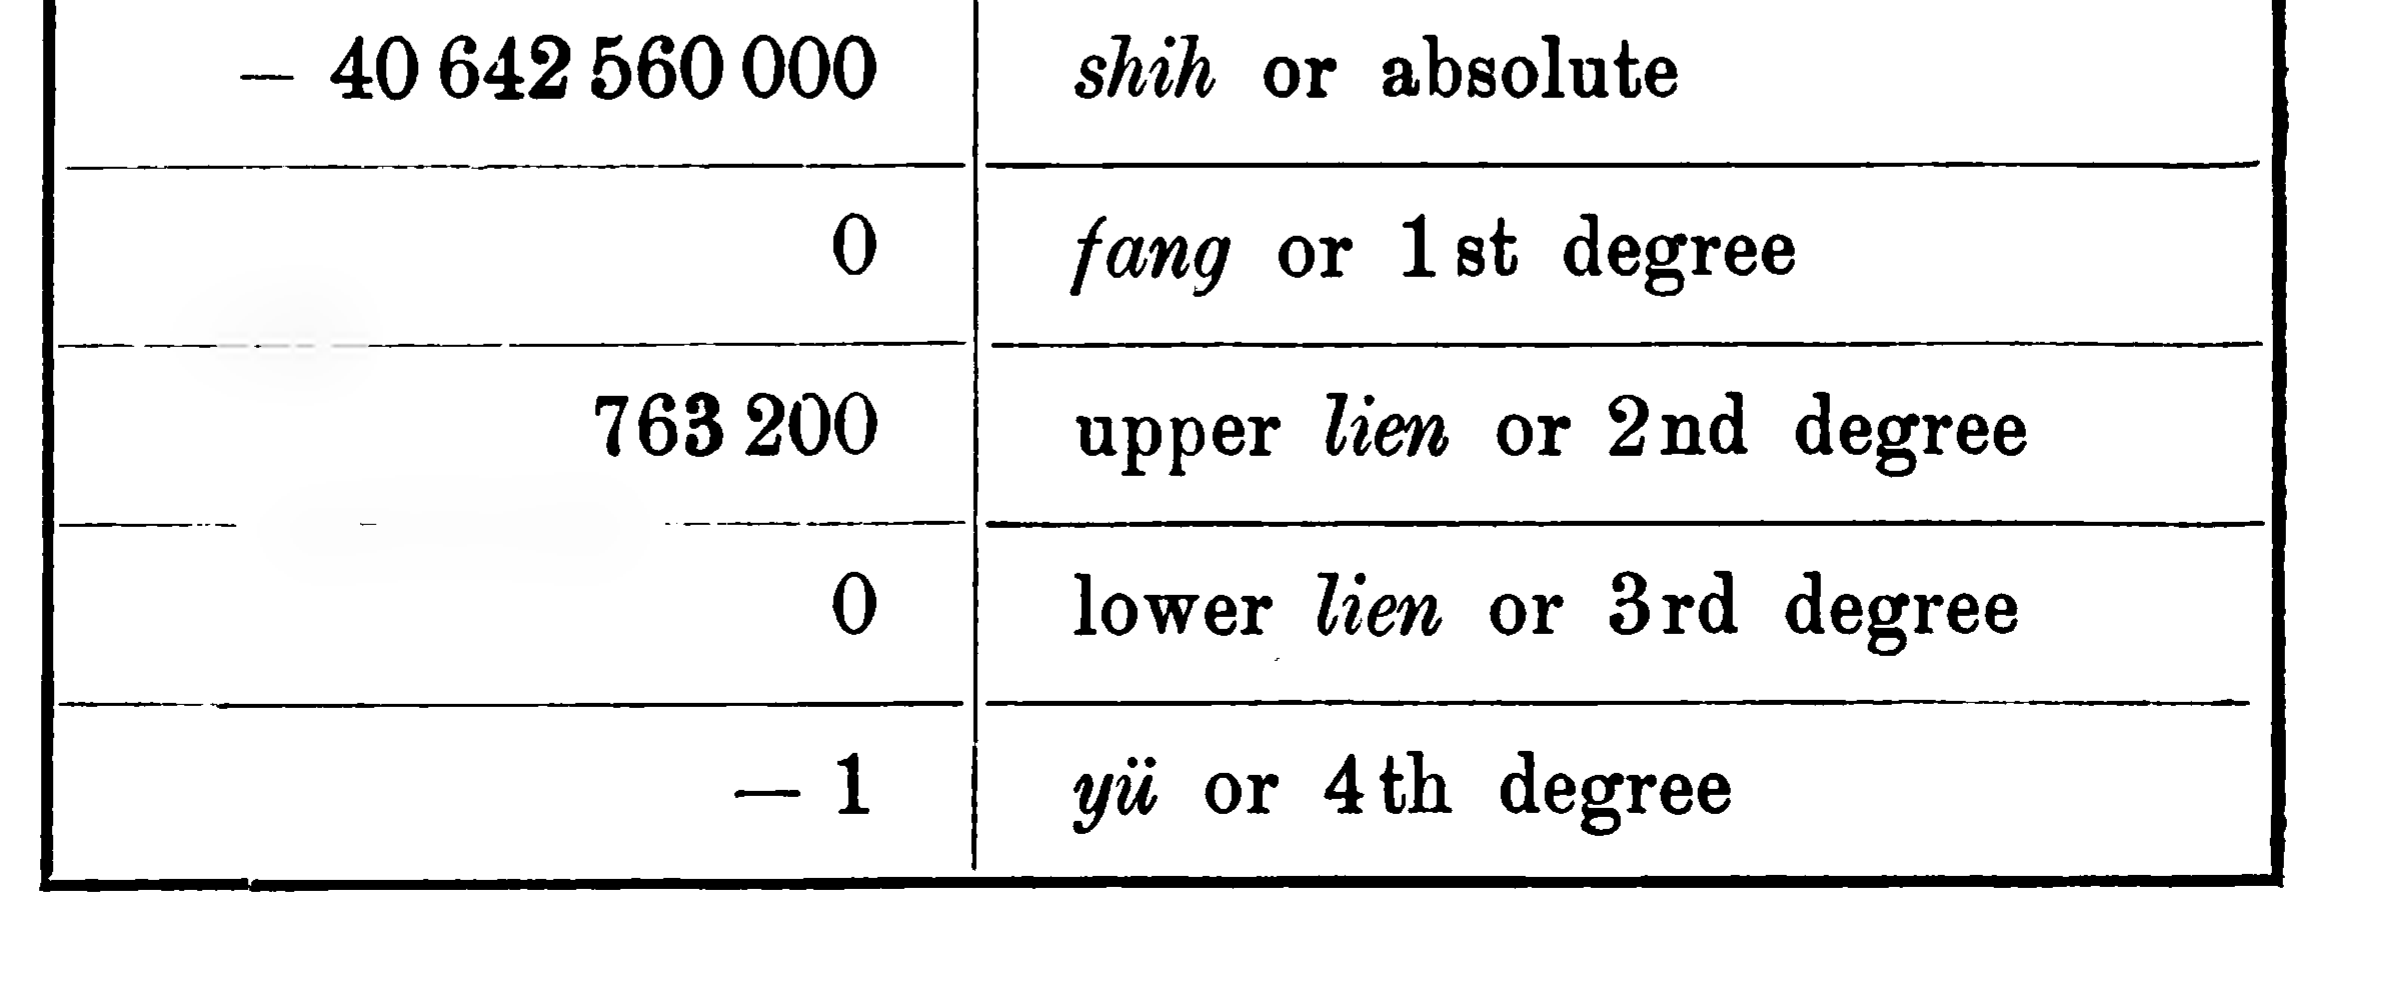
\includegraphics[width=0.94\textwidth]{pdf088-initial-root-arrangement.png}
\end{center}
\scanfooter

\scanpage{0089}{Chapter 11, printed page 75}
To carry out the evolution of the root the respective classes except the absolute must be removed to the left, as in the case of the extraction of the square and cube roots; these removals should be so effected that the 1st degree class is advanced by one column, the 2nd degree class by two columns, the 3rd degree class by three columns, and the 4th degree class by four columns. In the case before us, the same process must be repeated for the second time; and thus the root is known to be of three figures. Although the successive steps are indicated in Ch'in's work in separate diagrams, we shall here explain the process in an abridged form, because it is too tedious to reproduce all the passages followed by the author.

The first figure in the root will be seen to be 8, and this is to be multiplied by the 4th degree class and the result added algebraically to the 3nd degree class. Multiply this by the root and algebraically add to the 2nd degree class. Multiply the result again by the root and add algebraically to the 1st degree class. Multiply the root by this result and subtract from (or algebraically add to) the absolute class. The result is:

\begin{center}
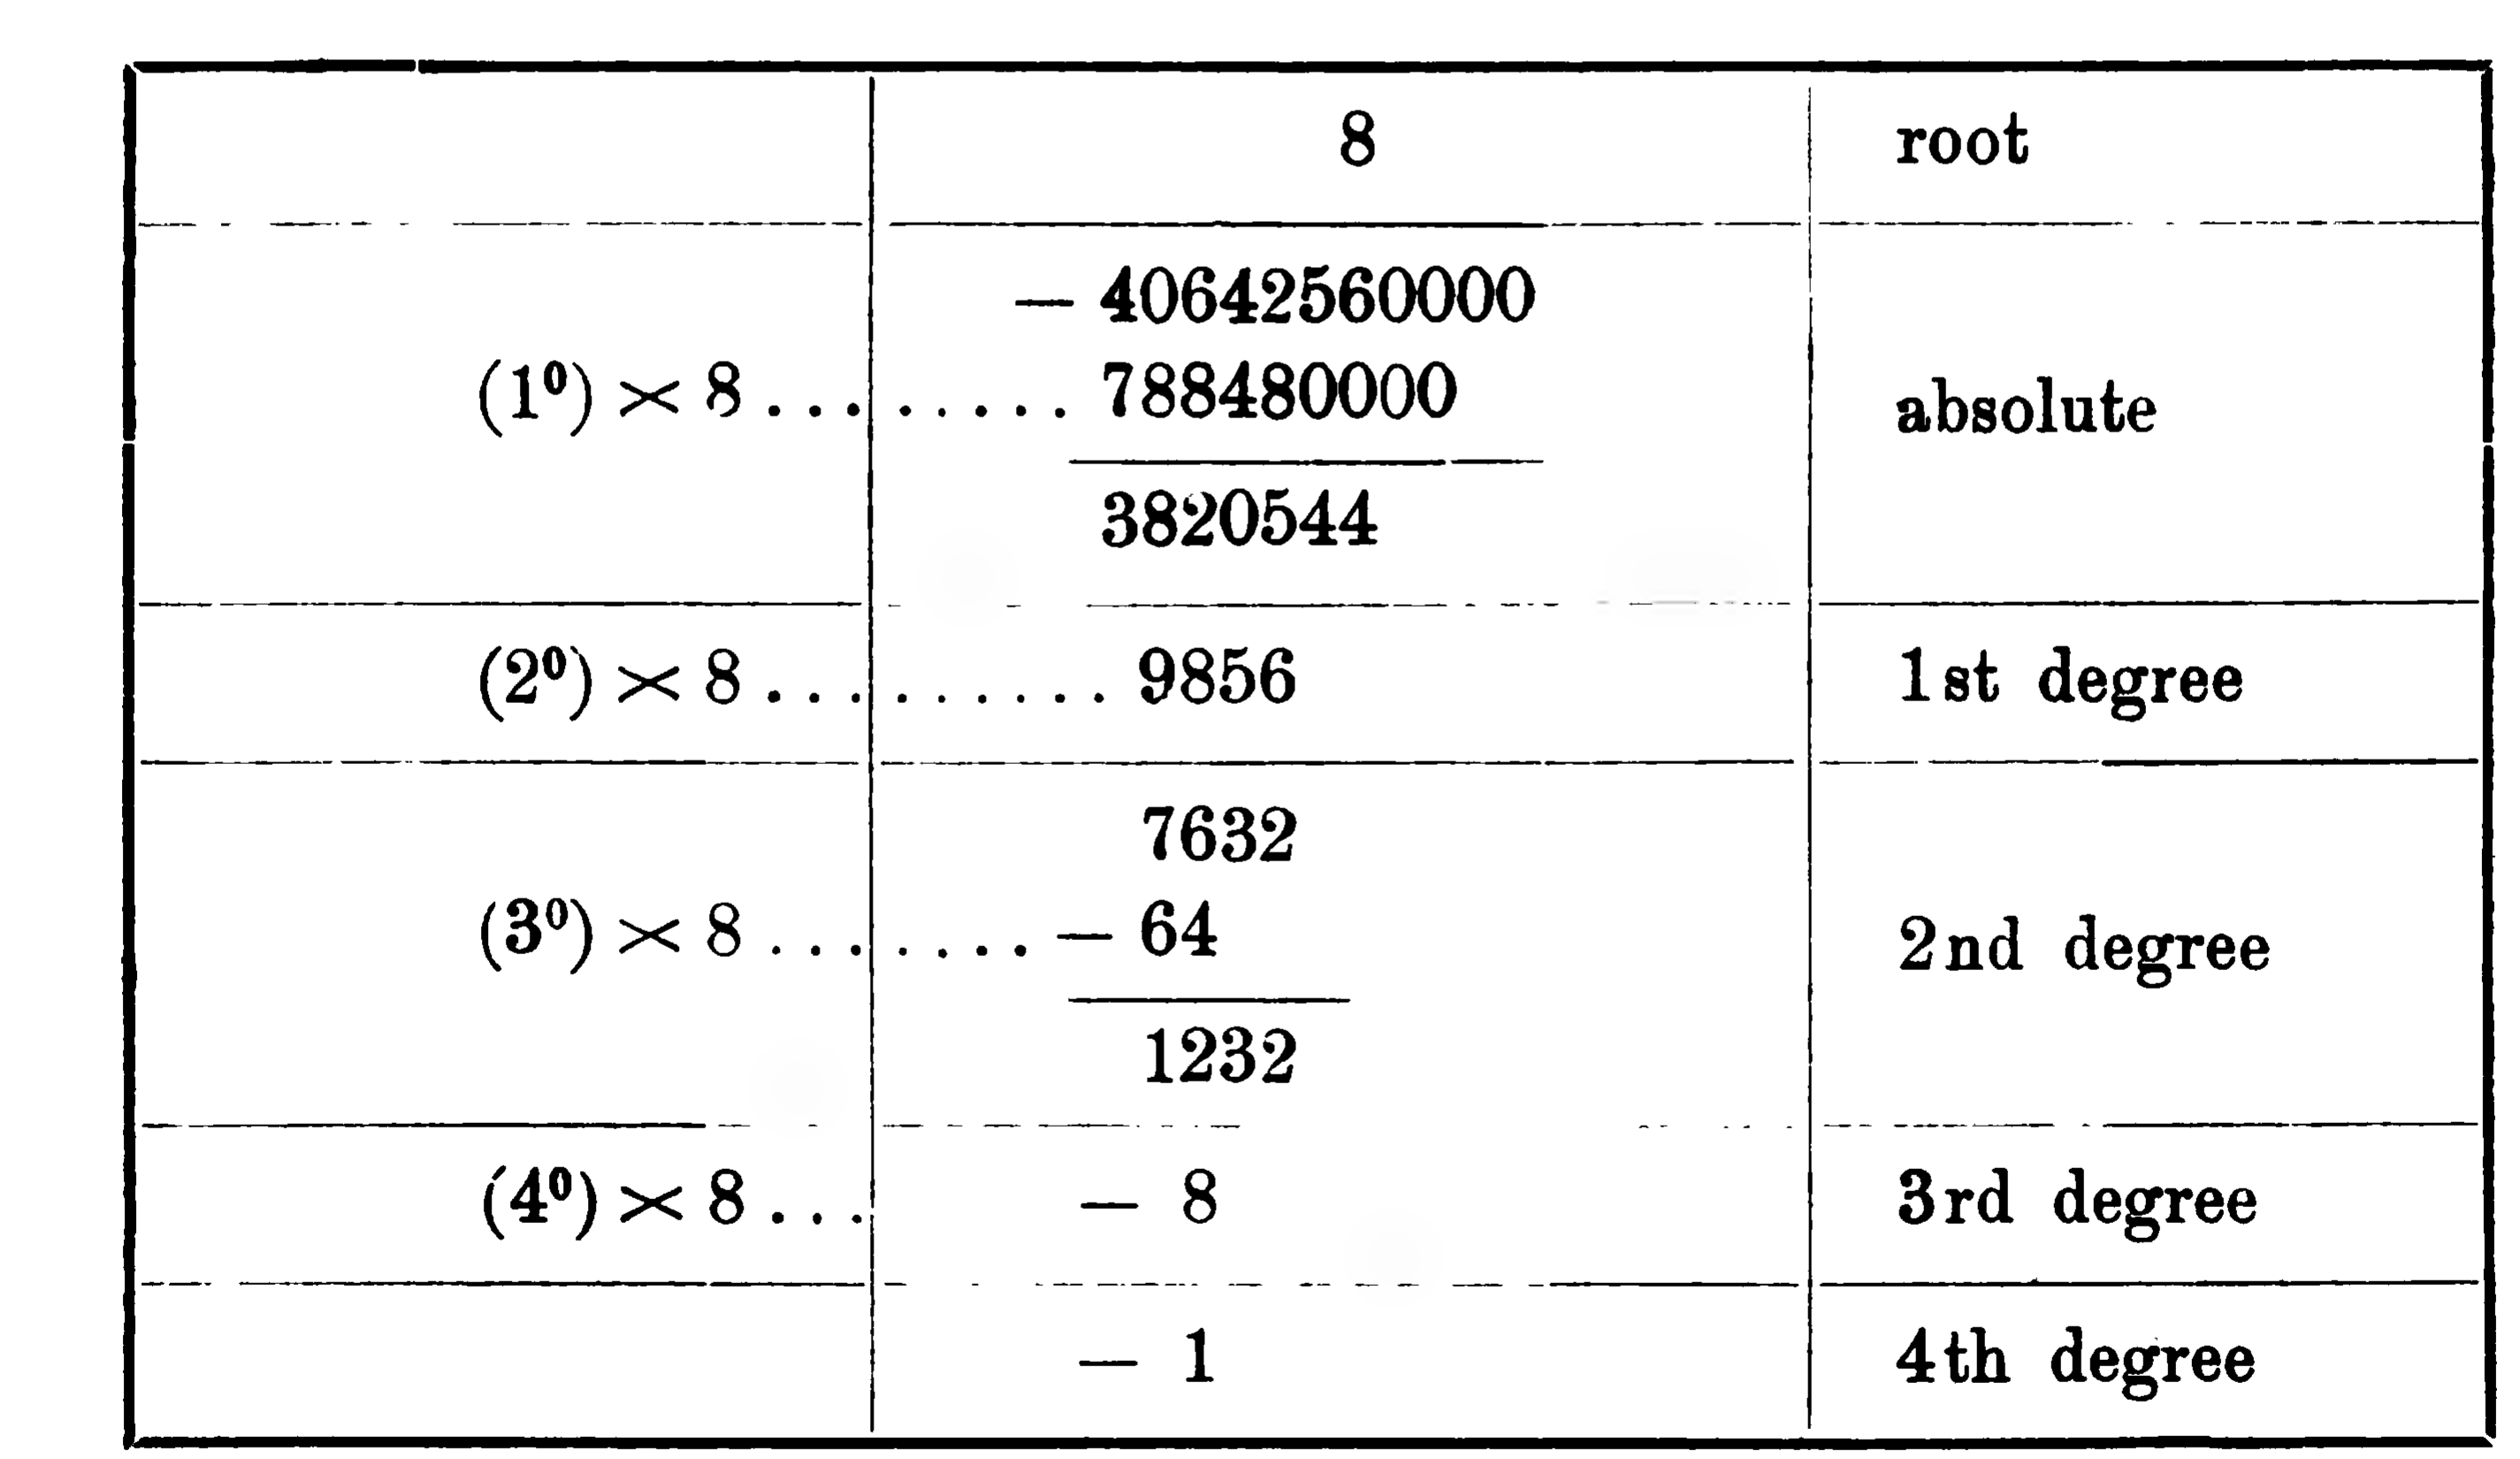
\includegraphics[width=0.94\textwidth]{pdf089-first-root-figure.png}
\end{center}

Now multiply the root by the 4th degree class in the newly obtained expression and add the product algebraically to the 3rd degree class. Multiply this result by the root and add the product algebraically to the 2nd degree class. Multiply by this result the root and add the product algebraically to the 1st degree class.
\scanfooter

\scanpage{0090}{Chapter 11, printed page 76}
Again multiply the 4th degree class by the root and add the product algebraically to the 3rd degree class. Multiply by this result the root and add the product algebraically to the 2nd degree class.

Again multiply the 4th degree class by the root and add the product algebraically to the 3rd degree class.

The result of these operations is as follows:

\begin{center}
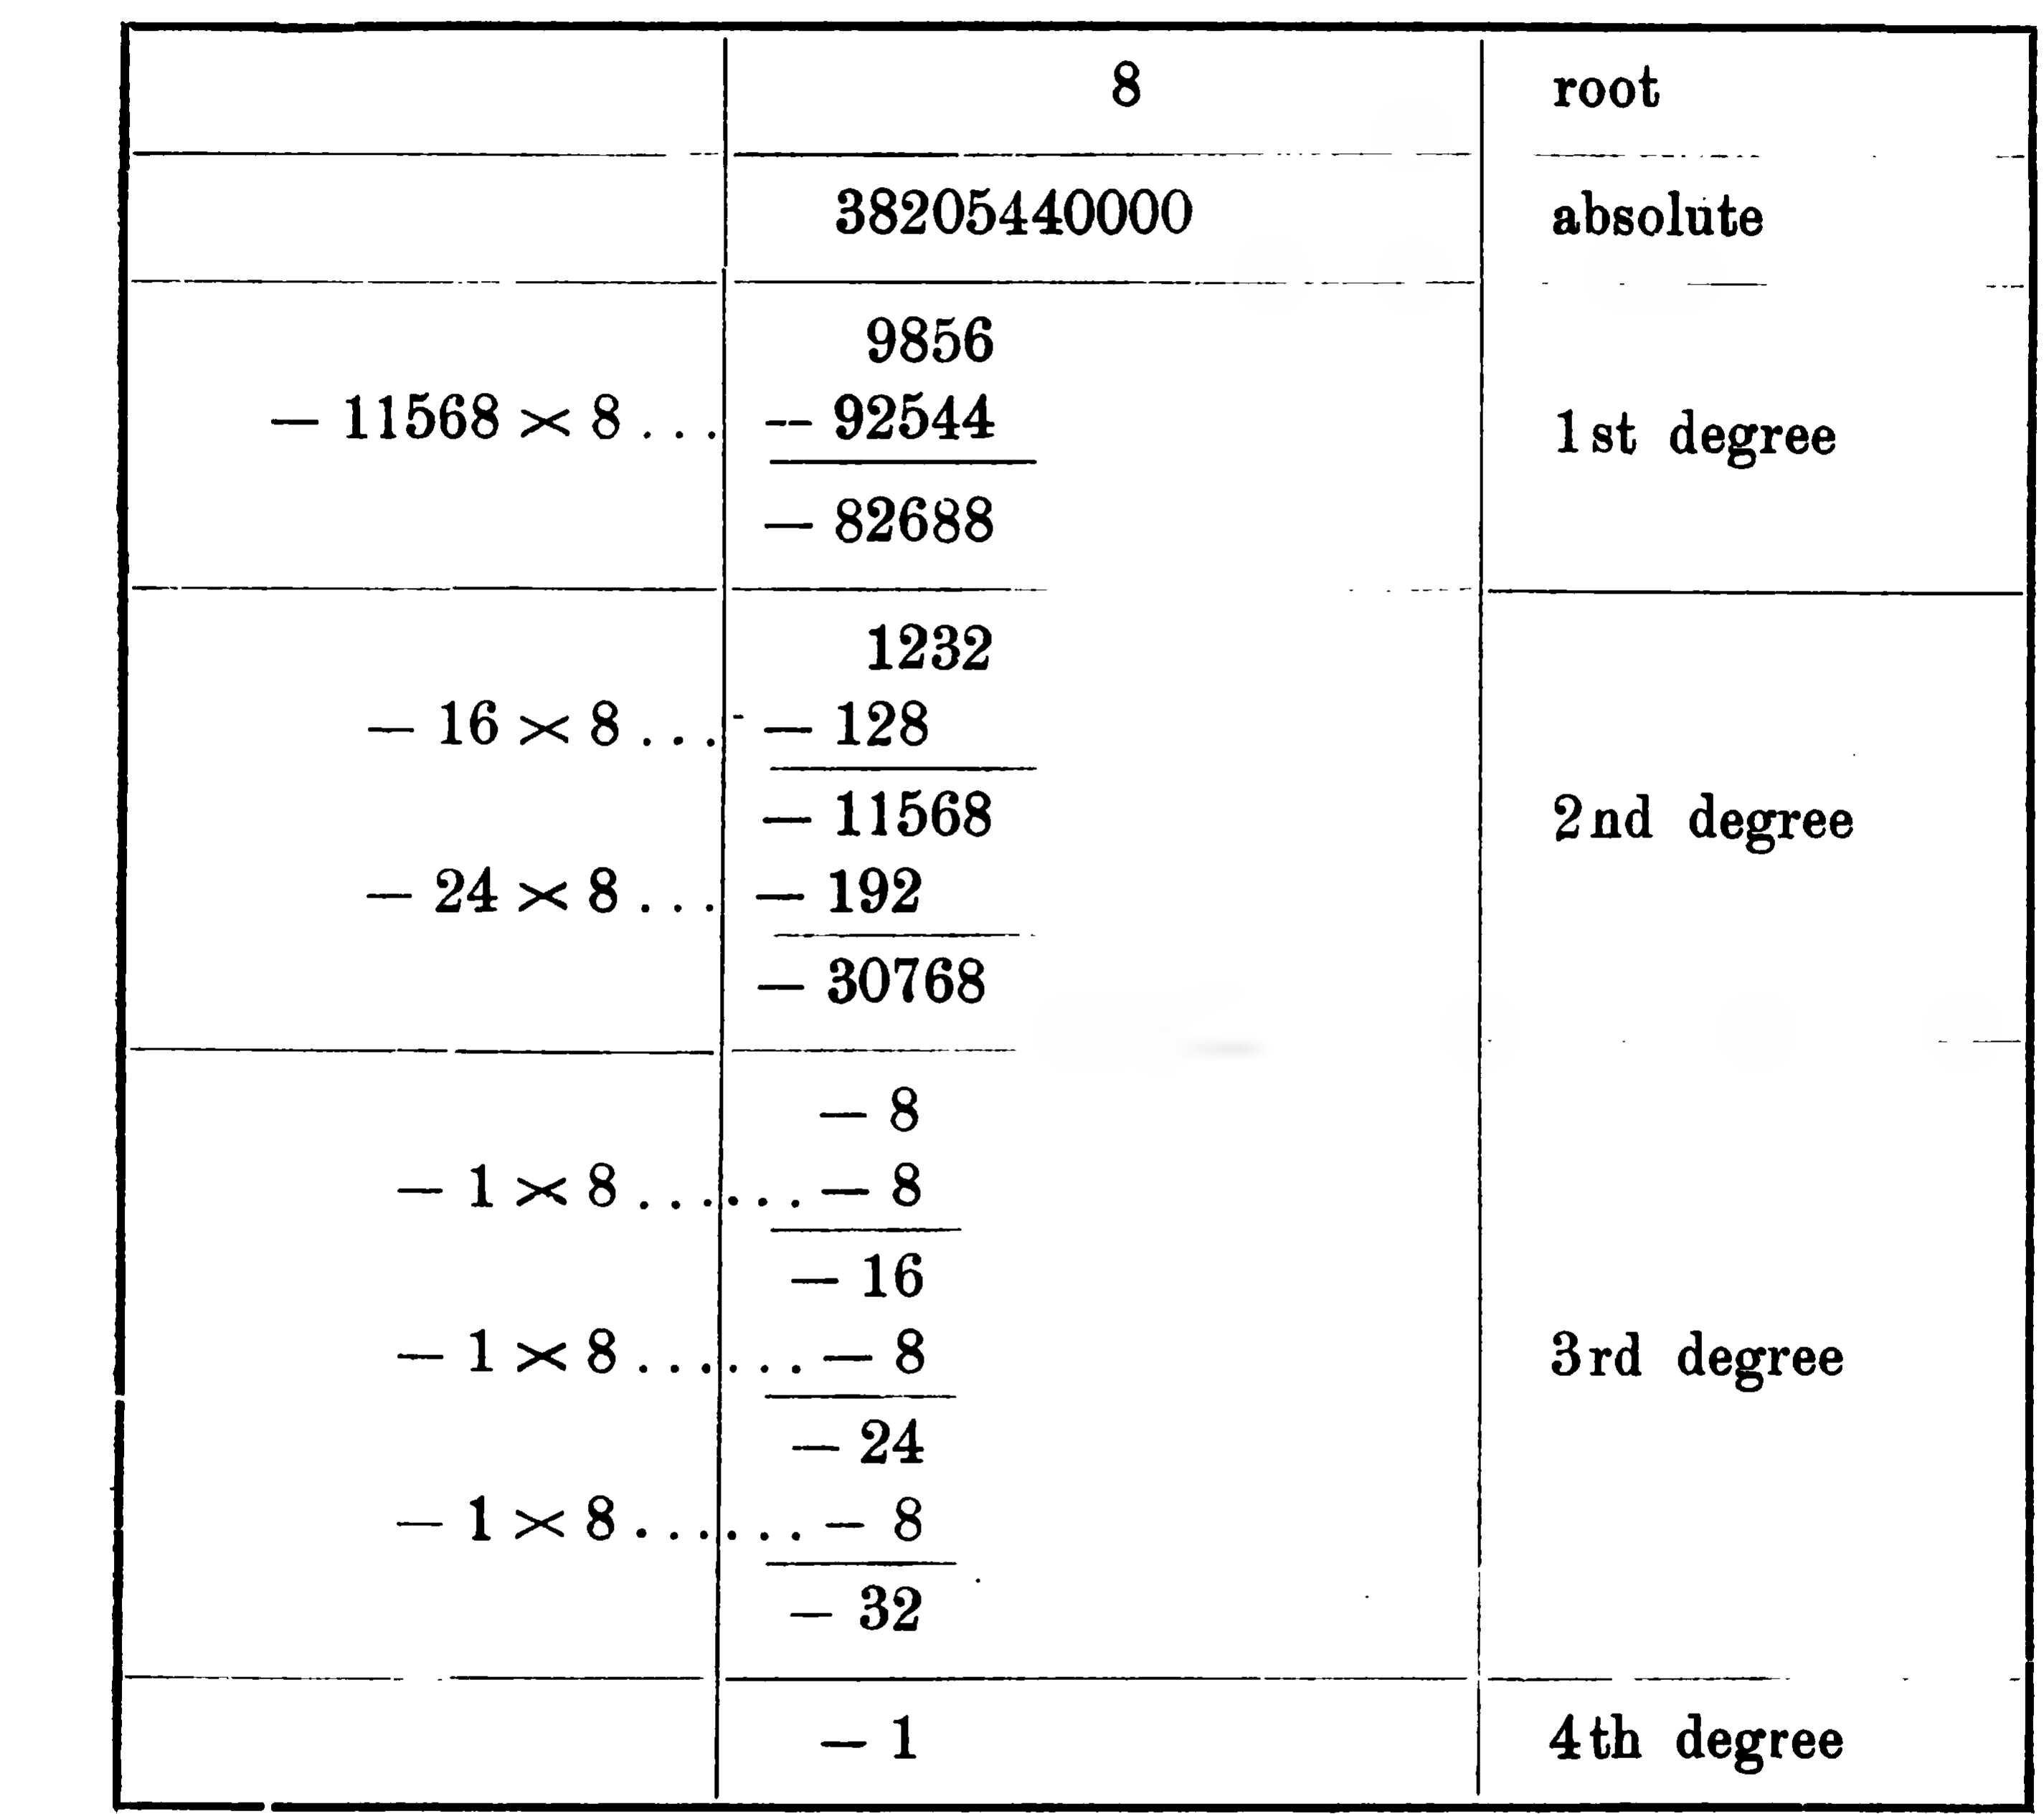
\includegraphics[width=0.92\textwidth]{pdf090-root-operations.png}
\end{center}

Next move back the 1st, 2nd, 3rd and 4th degree classes by 1, 2, 3 and 4 columns respectively to the right. Thus the arrangement assumes a form as shown on the next page.

Now taking 4 for the second figure in the root, proceed exactly in the same manner. Successive repetitions of like operations will lead to the evaluation of the further figures in the root. But in the case under discussion, the absolute class vanishes after the operation is effected for the second figure of the root, so that the evolution comes here to end, giving the root $=840$.
\scanfooter

\scanpage{0091}{Chapter 11, printed page 77}
In learning what the Chinese practised in extracting the root of an equation as we have described, we cannot but be reminded of the celebrated method of Horner for the approximate solution of numerical equations. See how identical the two are in their points of principle.

\begin{center}
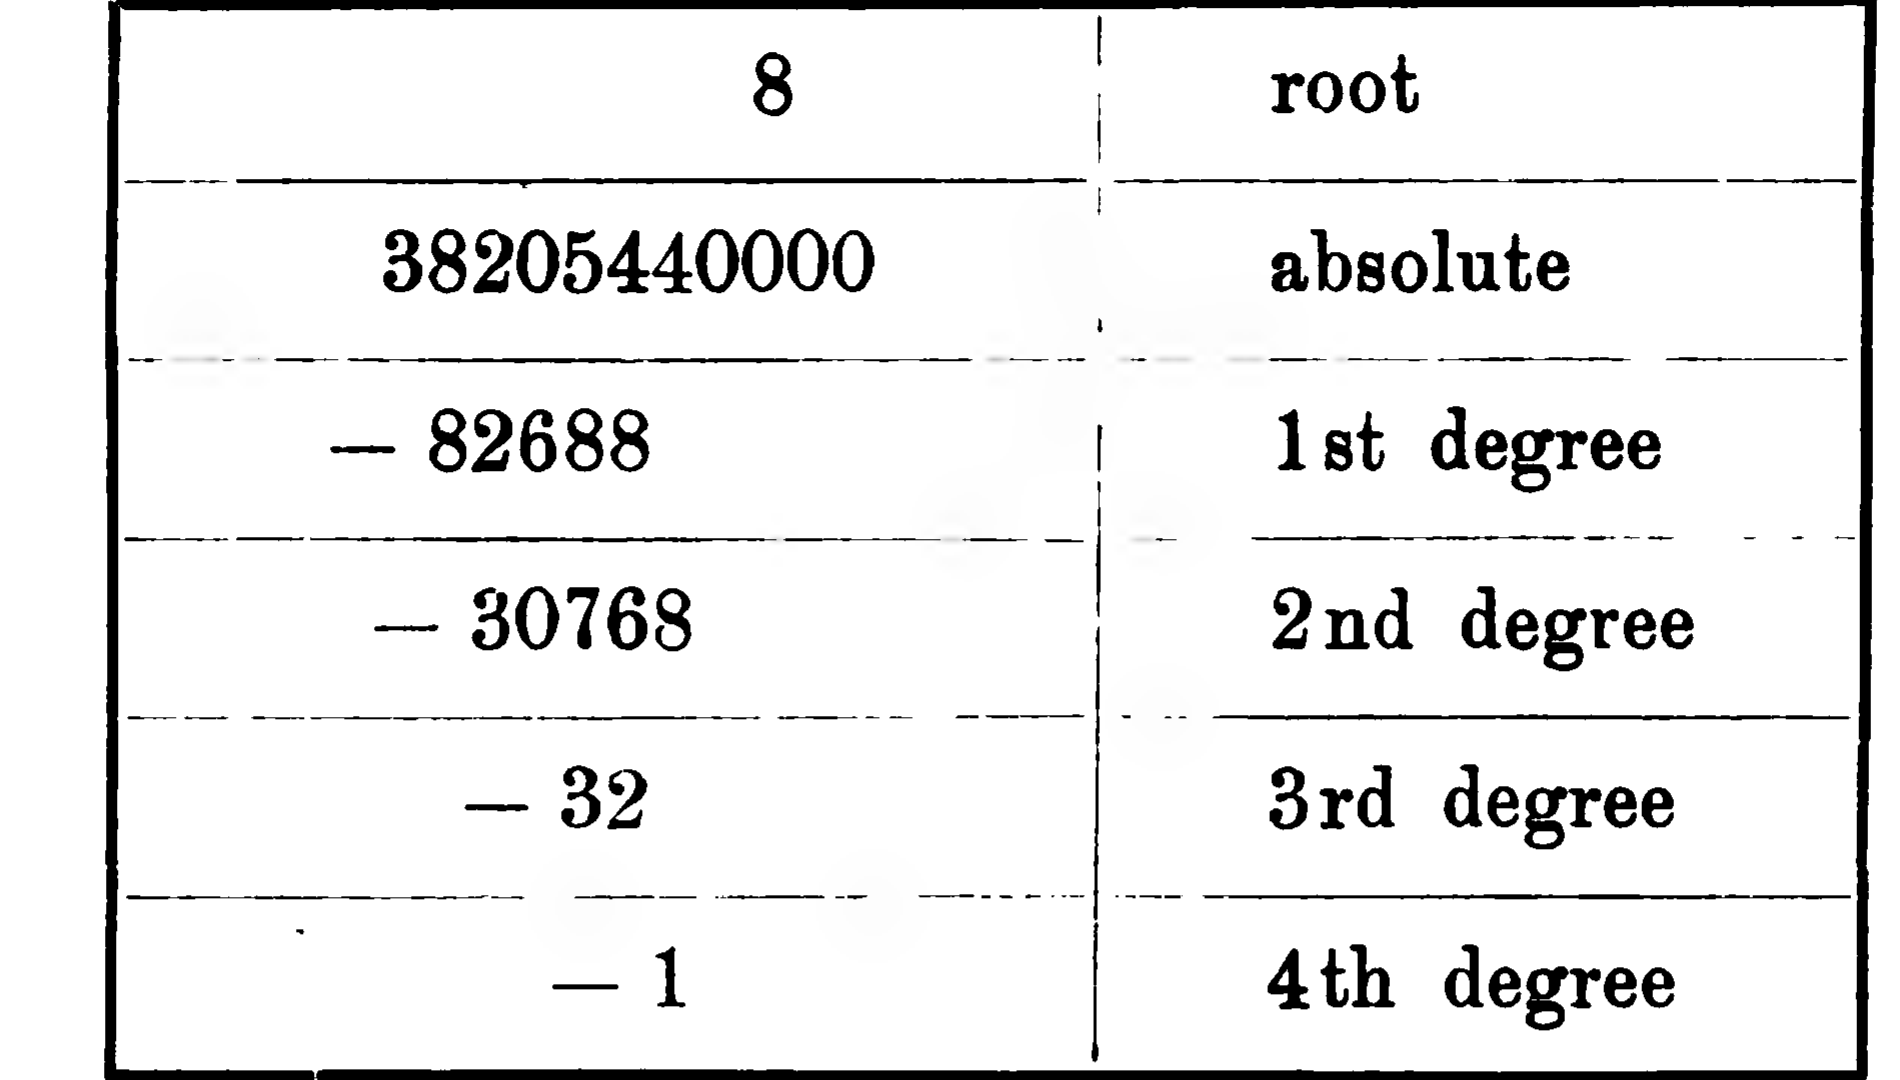
\includegraphics[width=0.68\textwidth]{pdf091-shifted-root-arrangement.png}
\end{center}

If there is anything that differs in the two methods, it should be sought for in the different ways of arrangement, which we owe naturally to the difference in the systems of operation. The Chinese solved their equations on the calculating board, while Horner applied a written mode of calculation. At any rate, who can deny the fact of Horner's illustrious process being used in China at least nearly six long centuries earlier than in Europe, for Horner's paper was published in 1819? We of course don't intend in any way to ascribe Horner's invention to a Chinese origin, but the lapse of time sufficiently makes it not altogether impossible that the Europeans could have known of the Chinese method in a direct or indirect way. Moreover the Europeans had been for more than two centuries in active cooperation with the Chinese to transplant the Occidental sciences into the land of the Middle Empire. Among them there were not a few who were versed in mathematics, Why could they not have come in contact with the method of the Chinese algebra, that lay openly before their eyes? As to the feelings of the Chinese upon the occasion of the European algebra or process of solving numerical equations being introduced into China in the 17th century, we shall return again to say something, when we discuss the mathematical attainments of the Chinese under the present Dynasty of Ching.

The process just described equally applies to the evaluation of the decimal part of the root, as later Chinese as well as Japanese mathematicians have done, but Ch'in did not try anything of the sort.
\scanfooter

\scanpage{0092}{Chapter 11 conclusion, printed page 78}
In the evolution of $\sqrt{1000}$ Ch'in gives the root to be $31\frac{13}{21}$, where the fractional part is derived in the same manner as is done in old times

He applies the same treatment to the case of equations. In the equation
\[
(a+b)^3\times10=\left\{\left(\frac a2\right)^2-\left(\frac b2\right)^2\right\}x+x^2,
\]
where $a=576$ and $b=34$, Ch'in first calculates the integral part of the root to be 21742, when there remains the quantity 10426 in the absolute class. Now Ch'in calculates the 1st degree class that is needed in the next operation; this quantity is found to be 126140. Here to find half the root, Ch'in takes the halves of these quantities and puts
\[
(\text{the root})=10871\frac{5213}{63070},
\]
where perhaps the denominator is erroneously halved.

It is a noted fact in history that Thomas Harriot (1560---1621) made all the significant terms in an equation stand on one side of the sign of equality. Ch'in arranged the absolute term so as always to be negative, which is much akin to the achievement of Harriot. Ch'in's contemporary Li Yeh and all other mathematicians in succeeding ages followed the same way of arrangement as indicated in Ch'in's work. In this point, therefore, the Chinese may be said to have been more than three centuries ahead of Harriot.

Notwithstanding that Ch'in Chiu-shao was very minute on the one hand in explaining the process of evolution or root extracting of numerical equations, on the other he utterly neglected the description of the way to construct such equations by algebraical considerations from the given data in the problems. This does not mean however that he was altogether foreign to algebraical treatments; or how could he have been led to these complicated equations he employed in his treatise? But the explanation of algebraical manipulations remained in the hands of his contemporary Li Yeh, who lived far apart in the contending monarchy of the Mongol invaders. We now pass on to review something of the life of this mathematician.
\scanfooter


\scanpage{0093}{Chapter 12 opening, printed page 79}
\setcounter{footnote}{0}
\begin{center}
CHAPTER 12.\\
LI YEH.
\end{center}
\phantomsection\addcontentsline{toc}{subsection}{Chapter 12. Li Yeh}

In 1248, the next year after Ch'in Chiu-shao's composition of the \emph{Su-shu Chiu-chang}, there appeared the \emph{T'sê-yüan Hai-ching} or the ``Sea-Mirror of the Circle-Measurements'' written by Li Yeh, and it was followed by his \emph{I-ku Yen-tuan} of 1259. These two works are as invaluable in history as we have esteemed Ch'in's work, for it is in them that we find the algebraical considerations explained for the first time by a Chinese hand, in so far as old documents are handed down to us. It is highly worthy of notice that Ch'in solely concentrated his attention upon the explanation of the process of solving the equations obtained without giving any slightest hint as to their construction, while Li merely tried to describe, if not sufficiently, how to proceed from the given data in the problems to the construction of the equations required in their solution, without giving the actual method of solving them. Does it not then appear as if Ch'in and Li had come forth at the same juncture of time to cooperate in sufficiently furnishing to the Chinese algebra its requisite establishment? Nevertheless the two lived far apart, and indeed in different and contending monarchies.

Although the \emph{Sung-Shih} or the ``Historical Records of the Sung Dynasty'' does not give Ch'in's biography, the \emph{Yuen-Shih} or the ``Historical Records of the Yuen Dynasty'' contains a life of Li Yeh in the Biographical Section of the book. According to this record, Li Yeh\footnote{Li Yeh is sometimes represented as Li-yeh Jin-king (as by Moritz Cantor) but his family name was Li and his personal name Yeh; Jin-king was his familiar name, or surname, which all Chinese persons bear.} was born at Luan-ch'êng under the yoke of the Monarchy of Chin that was situated in the north of China and that was ever in strife with Sung. He passed the examination of the Chin government for the civil service and he was made after some time the governor of Chün Chou, when in 1232 the castle of the province fell into the enemy's hands. Li escaped in disguise and lived in poverty; he then gave himself to the studies of books, which he could collect. After the overthrow of the Chin Monarchy\footnote{The Monarchy of Chin was overthrown by the Mongolian invaders in 1234.}, the Mongolian prince Kublai Khan sent for him, because he had learned of his wiseness Asked by the mighty prince of the wise men of the times, Li Yeh promptly replied: ``The world is never destitute of wise men. If you will seek
\scanfooter

\scanpage{0094}{Chapter 12, printed page 80}
after them, they will be before you. If however you don't seek, there comes no wise man at all. This is for only an obvious reason''.

Asked again of the discretion of governing the state, Li Yeh earnestly told the prince that he ought to promote virtuous men and get rid of unvirtuous; that he must strictly observe regulations and keep order. He was not even afraid of expressly speaking about the evils of the times.

Li Yeh's replies were all approved by Kublai Khan and he was held in great esteem; but he did not serve the Mongolians at that time.

In his life's decline Li Yeh lived in a Mongolian territory, where he taught pupils, who became more and more numerous in course of time. On Kublai Khan's ascending the throne in 1264, Li was again sent for; he again declined to accept service on account of his age and infirmity. But in the next year he was obliged by repeated entreaties to occupy a chair in the Han-lin Academy. Being there for only a few months, he resigned his post and went away. He then died at the age of 87. Some later writers --- among them Chiao. Hsün who flourished at the end of the 18th century and at the beginning of the following century may be mentioned --- take the year 1265 as the date of Li Yeh's death.

According to the ``Historical Records of the Yuen Dynasty'', Li Yeh left besides the two works already mentioned other writings such as the \emph{Ching-chai Wen-chi} or ``Collections of Ching-chai's Writings'', Ching-chai being Li Yeh's nom-de-plume, consisting of 40 books, the \emph{Pi-shu Su-hsiao} consisting of 12 books, the \emph{Fan-shuo} consisting of 40 books, the \emph{Ku-chin Nan} or ``The Old and Modern Times Criticised'', that consisted of 40 books, etc.

The ``Sea-Mirror of Circle-measurement'' was intended, as the title indicates, to treat of measurements connected with a circle, although the treatment does not lie in the domain of the quadrature of the circle. As the author writes in the preface of this work, he was used to mathematical studies from his youthful days and it was always his regret that there was not anything settled about the calculations referring to a circle; so for instance, the old value of $\pi$ and the values of Liu Hui and of Tsu Ch'ung-chih all differed; while there was no process with which arcs, sagittae, and segmental areas of a circle could be measured in such a way as was satisfactory to him. After he was 54 years of age, however, he came upon the doctrine of the \emph{T'ung-yuen Chiu-yung}, which proved highly interesting to him. This was perhaps
\scanfooter

\scanpage{0095}{Chapter 12, printed page 81}
the way of algebraical considerations of the celestial element. But to tell the truth, subsequent native writers are all at a loss to make clear the meaning of this term. In any case Li Yeh cultivated the doctrine or art thus brought before him with great care and he was at last satisfied about the questions that had troubled him so long.

With such preparatory remarks Li Yeh proceeds in the twelve books or chapters of the ``Sea-Mirror'' to establish his rules. In the opening of the treatise he first gives a diagram which is as shown in the figure.

\sourceasset{0.47\textwidth}{pdf095-li-yeh-diagram.png}

In the first book or chapter Li Yeh describes the relations of the various parts in this figure, and the 2nd and further books are devoted to the consideration of various rules of calculation in relation to these quantities. The treatment is done in the algebraical way.

The same author's subsequent composition, the \emph{I-ku Yen-tuan} was also devoted to algebraical treatment. The ways of representing algebraical expressions are however different in these two works.

We have already remarked upon Ch'in Chiu-shao's employment of the term \emph{t'ien-yuen}, which means celestial element. This same term was also employed by Li Yeh. Ch'in referred to the celestial element in his treatment of indeterminate problems, as we have said; he did not however employ the term in connection with his manipulation of numerical equations, with which he has become so prominent in history. It was in this latter connection that Li Yeh used the term celestial element.

In the algebraical process of Li Yeh's celestial element, unity is employed as the representative of an unknown number. This was certainly done with the aid of a calculating piece. But in writing in his work Li uses the ideogram \emph{yuen} or element written by the side of it to distinguish it from other terms in an expression, which are arranged in a vertical column. The absolute term comes under the linear term and it is marked by the ideogram \emph{tai}, perhaps implying the meaning that it is in the place of the \emph{tai-chi} or extreme limit or great extreme. The square of the celestial element is arranged imme-
\scanfooter

\scanpage{0096}{Chapter 12, printed page 82}
diately above the element; next above comes the `cube; and so on upwards. Thus the equation
\[
x^3+15x^2+66x-360=0
\]
would be written as given annexed.

\sourceasset{0.54\textwidth}{pdf096-equation-arrangement.png}

The square and further terms are not expressly indicated, but these are designated by the relative positions to the great extreme or the absolute term. In practice the two ideograms \emph{yuen} and \emph{tai} are not necessary; one of them may be advantageously omitted.

Li Yeh's way of arranging equations as found in the ``Sea-Mirror'' is utterly different from that of Ch'in, who had followed the development of the root-extraction process of old times. It is utterly unknown however to us as to what reason or reasons had induced our author to adopt such an arrangement. But in the \emph{I-ku Yen-tuan} Li Yeh changes his arrangement in the same way as Ch'in has done, bringing the absolute term uppermost and other terms successively below it. And this way was destined to prevail thenceforth.

Ch'in Chiu-shao distinguished positive and negative numbers by writing the former in red and the latter in black colours. This was very natural, whether invented by Ch'in himself or otherwise, because the Chinese had been accustomed long before to use red and black calculating pieces to distinguish positive and negative numbers, and the equations were ultimately to be arranged with these pieces. But it is not convenient to use two different colours in writing and especially in the case of printing. Thus there soon arose the usage of distinguishing numbers of different signs, when representing them in writing, by referring to a specially designed symbol. Such a symbol is met with in both works of Li Yeh. If we are not sure whether he was the first Chinese who used the symbol, yet his works are perhaps the oldest writings wherein it was made use of, that are transmitted to our time. This symbol consists of a diagonal stroke drawn through the right-hand figure. Thus

\sourceasset{0.73\textwidth}{pdf096-negative-numeral-forms.png}

stand respectively for $-10724$, $-9$ and $-10200$.
\scanfooter

\scanpage{0097}{Chapter 12, printed page 83}
The symbol $\bigcirc$ for the cipher was equally employed by Ch'in and Li.

This symbol of zero, together with Li Yeh's way of designating negative numbers, have been employed constantly ever since. The Japanese mathematicians in feudal times also had recourse to these symbols.

Ch'in Chiu-shao and Li Yeh were contemporary scholars and taught the treatment of equations at the same time. This has caused some scholars to think of the latter as having been influenced by the treatise of the former. But the majority of later native scholars appear to have agreed in considering the productions of the two mathematicians as worked out independently of each other, because they lived far apart in rival monarchies. For our part we acquiesce in this opinion. But the agreement of the two scholars in their employment of the same term of the \emph{t'ien-yuen} or celestial element and the same symbol $\bigcirc$ for cipher awaits an explanation, for such could in no way originate from the simultaneous inventions of two independent workers. It will be meet for us therefore to conclude that the practice of the celestial element as well as the use of the cipher symbol had existed from before the time of these scholars. The zero symbol was perhaps introduced from India during the reign of the T'ang Dynasty. What Ch'in and Li themselves record in the prefaces of their works seems to justify our view, although very scantily.

We shall say something in the next chapter about the works of a contemporary scholar, whose writings are dated a little subsequent to our authors and who also treats of the same matters.

Half a century later there appeared a mathematician whose name was Chu Shih-chieh, who wrote the \emph{Szu-yuen Yü-chien} in 1303. According to the preface of this work, we learn that there had been a certain Yuen Hao-wen, who was a civil officer in the Chin Monarchy. After the fall of that Empire, he spent his days in writing on various subjects, and he was versed in mathematics and especially in the method of the celestial element. He was a friend and an intimate one to Li Yeh. Yuen once wrote detailed notes on a mathematical treatise entitled the \emph{Ju-chi Shih-hsiao} written by one Liu Ju-hsieh. This was most certainly a treatise on the celestial element algebra, but neither Liu's original work nor Yuen's notes exist now. Nor do we know of Liu's life-time.

The algebra of the celestial element was certainly no new invention in the 13th century; it seems it had descended from former ages.
\scanfooter

\scanpage{0098}{Chapter 12 conclusion and Chapter 13 opening, printed page 84}
But it was equally true that the celestial element was not popularly practised in those times among the whole circle of mathematicians. Even the single fact that Li Yeh changed the way of arrangement he had formerly employed in a later composition may well illustrate that such a usage had not been a very common one among his contemporaries. See how Li Yeh had put a stress on his ``Sea-Mirror'', when he recommended the treatise to his son on his death-bed! According to Wang Tê-yüan who reprinted the ``Sea-Mirror'' in 1287, Li Yeh bade his son burn all his writings on his death, except the one treatise, the \emph{T'sê-yüan Hai-ching}, or the ``Sea-Mirror'', saying he was aware that posterity would doubtless come to revere its contents.

In any case the Chinese algebra had sprung from the old practice of considering the extractions of square and cube roots. The Chinese algebra as treated by Li Yeh and his successors was manipulated on the board for calculating pieces, which was the peculiarity of the Chinese mathematics. We have no reason whatever to suspect the Chinese of borrowing their way of algebraical manipulations from any foreign source.

In the next chapter we shall speak of another mathematician in whose works we meet again with the equations of the celestial element.

\begin{center}
CHAPTER 13.\\
YANG HUI.
\end{center}
\phantomsection\addcontentsline{toc}{subsection}{Chapter 13. Yang Hui}

Immediately after the appearance of the treatises of Ch'in Chiu-shao and Li Yeh there came out a third mathematician whose name was Yang Hui. He was a native of Ch'ien-t'ang and belonged to the Sung Monarchy. We know little or nothing of his life, but we are possessed of several of his writings preserved to our own days. These writings are the \emph{Hsiang-chieh Chiu-chang Suan-fa} or ``The Analysis of the Arithmetical Rules in the Nine Sections'', 1261, in which some of the rules and problems in the old Nine Sections are explained; ``The Supplements to the Analysis of the Nine Sections''; and five others called by Yüan Yüan as \emph{Yang Hui Suan-fa} or ``Yang Hui's Arithmetical Works'', one of which bears the date of 1275.

In the ``Analysis of the Nine Sections'' Yang Hui illustrates the summation of an arithmetical progression. To find the total distance traversed in fifteen days by a steed who goes 193 Chinese miles (\emph{li}) on the first day and who increases his speed 15 miles every day, Yang
\scanfooter

\scanpage{0099}{Chapter 13, printed page 85}
takes the product of the number of days and half the sum of the first day's speed and that of the last day, which is found by adding to the former 14 times one day's increase of speed. Here he adds a diagram as shown annexed.

\sourceasset{0.68\textwidth}{pdf099-speed-diagram.png}

It is obvious that Yang intends to show that the required answer is obtained by taking a quantity corresponding to the area of the rectangle composed by twice this figure, and halving the result.

In the \emph{Suan-fa T'ung-pien Pen-mo} Yang Hui further gives the formulae for the sums of the progressions he calls the triangular and the square, which are
\[
1+(1+2)+(1+2+3)+\cdots+(1+2+3+4+\cdots+n)
=\frac{n(n+1)(n+2)}{6},
\]
\[
1^2+2^2+3^2+\cdots+n^2
=\frac{1}{3}n\left(n+\frac{1}{2}\right)(n+1).
\]

About these progressions the formulae, or rather rules that lead to these formulae, alone are given; no explanation is tried as to the analysis of them.

As we have said the \emph{Wu-tsao Suan-ching} gives the area of a quadrilateral erroneously as the product of the half sums of the two pairs of opposite sides. Yang Hui was aware of the incorrectness of it, and he tried to correct it in the ``Supplement of the Analysis''. He considers a quadrilateral whose sides are successively 35, 15, 45, 25. He calculates its area by dividing it into two parts by a perpendicular let fall from the vertex of the sides 35 and 25 upon the side 45. The perpendicular is taken to be $22\cdot44995$, and the two parts are treated as a right triangle and a trapezoid. Though this relation holds good only when the sides 15 and 45 are at right angles, yet the author does not make any remark as to the existence of other possibilities.

Yang Hui considers in the ``Supplement'' problems in simple proportion, one of which is this: ``A runs 100 paces ($a$), while B runs 60 paces ($b$). If now B starts 100 paces ($c$) ahead of A, in how many paces will the latter overtake the former?''
\scanfooter

\scanpage{0100}{Chapter 13, printed page 86}
This problem may be obviously solved by the formula of proportion:
\[
a:a-b=c:x,
\]
which is the very formula Yang Hui employs. He only writes it in the form as annexed and cross multiplies two of the elements and divides the result by the remaining element.

\sourceasset{0.24\textwidth}{pdf100-proportion-cross.png}

Problems in proportion were considered in the ``Nine Sections'' but this scheme of expressing a proportion was given for the first time by Yang Hui, so far as our limited knowledge goes. He calls proportion by the name \emph{hu-huan}, which means literally ``alternate exchange''. He considers in his \emph{Hsü Ku-chai-ch'i Suan-fa} also problems in compound proportion, which he calls \emph{chung hu-huan} or ``doubled alternate-exchanges''.

In linear equations Yang considers problems where four. or five unknown quantities come in..

In the ``Supplement to the Analysis'' Yang considers the problem: ``There is a rectangular field whose breadth is 24 paces and $3\cdot4$ feet and whose length is 36 paces and $2\cdot8$ feet. What will be its area?'' In this problem there is of course nothing that is worthy of notice, but Yang's consideration of it is full of interest. He first treats it expressing the two lengths in terms of the tenth of a foot, but he also tries to carry out the multiplication in this way: When expressed by the decimal parts of the pace, the breadth becomes $24\cdot68$ and the length $36\cdot56$ paces. If we multiply these together we get
\[
24\cdot68\times36\cdot56=902\cdot308.
\]
This shows very well that Yang Hui had been in possession of a way of manipulating directly decimal fractions.

Yang Hui describes in his \emph{Ch'ong-ch'u T'ung-pien Suan-pong} division by the employment of the division-table which is made like the multiplication-table. This table is a part of what has been employed in later years in the arithmetic with the \emph{suan-pan} or the \emph{soroban} of the Japanese. We are not however informed as to whether he had practised his calculation on this sort of abacus. Of the origin of the \emph{soroban} we shall see later on.

In the old ``Nine Sections'' we find the problem: ``There is a door whose height is $6\cdot8$ feet greater than its breadth and whose diagonal length is 10 feet. What will be the length and breadth?'' This is just to find the two sides of a right triangle, whose hypotenuse $c$ and
\scanfooter

\scanpage{0101}{Chapter 13, printed page 87}
the difference $d$ of two sides $a$ and $b$ are given. To solve it Yang Hui makes use of the relation
\[
c^2=2a^2+4\times\left(\frac{d}{2}\right)^2+4\left(\frac{d}{2}\times a\right),
\]
which may be easily verified. This is capable of being respresented graphically as annexed.

\sourceasset{0.43\textwidth}{pdf101-square-relation.png}

If we subtract $2\times\left(\frac{1}{2}d\right)^2$ from the whole and take the half of the remainder, the result is the square of $a+\frac{1}{2}d$. We have therefore
\[
a=\sqrt{\frac{1}{2}\left\{c^2-2\left(\frac{1}{2}d\right)^2\right\}}-\frac{d}{2}.
\]

For this problem Yang Hui tries a second mode of solution. Thus from the relation $c^2=2a^2+2da+d^2$ follows
\[
c^2-d^2=2(a^2+da)\qquad\text{or}\qquad a^2+da=\frac{1}{2}(c^2-d^2),
\]
to which the method of evolution with an additive term applies, i. e., the approximate solution of the numerical equation of the second degree can be employed to obtain the value of $a$.

This method of evolution is explained graphically in the ``Supplement to the Analysis'' for the case of a quadratic equation, being referred to as taken from Liu I's \emph{I-ku Kon-yüan}. Yang employs several problems for that purpose and considers several cases separately; but we shall give only one of these cases.

``There is a rectangular field, 864 square paces in area, whose breadth is 12 paces less than the length. It is required to find the breadth.''

Here we have $A=lb=(b+d)b$, where the meanings of the letters employed will be obvious. Consequently $b=$ breadth is to be obtained from
\[
-864+12x+x^2=0.
\]

A method had indeed existed from old times for the solution of such an equation as this, as we have already observed. But Yang Hui explains how such a way is to be followed. Namely, if we know beforehand that $b=24$ and $l=36$ paces, the area of the rectangle will consist of such parts as shown in the left of the figures. Suppose therefore we take $x=20$ and operate as in the case of the extraction
\scanfooter

\scanpage{0102}{Chapter 13, printed page 88}
of a square root, then we shall see that the area may be divided as in the right-hand figure.

\sourceasset{0.67\textwidth}{pdf102-root-extraction-areas.png}

If we subtract therefrom $20^2$ and $20\times12$, the remainder will be $=2\times(20\times4)+12\times4+4^2$. Hence trying to divide roughly the remainder by $(20\times2+12)$, we see that the next figure in the evolved root should be 4. If we now subtract $4^2$, there is no remainder for the present case, and we find the breadth to be 24. If however there still is a remainder, the same process may be continued further.

Yang Hui also gives a case of a bi-quadratic equation. In the problem of finding the chord and altitude of a circular segment whose area ($a$) is 32 and whose diameter ($d$) is 13 he gives the equation
\[
-(2a)^2+4ax^2+4dx^3-5x^4=0,
\]
or
\[
-4096+128x^2+52x^3-5x^4=0
\]
for the determination of the altitude. The solution of this equation is briefly explained and the root is given to be $x=4$. This consideration is indicated by Yang as taken also from Liu I's work above referred to. No explanation is tried as to the analysis of the problem. The symbol $\bigcirc$ for cipher is used in this place, but positive and negative numbers are distinguished by words as done by Ch'in Chiu-shao.

It is very noteworthy that Yang Hui refers to Liu I's work in his considerations of equations but does not mention Ch'in Chiu-shao and Li Yeh. He was certainly independent of them. Liu I was a mathematician from whom Yang received instruction and so he belonged to the middle of the 13th century; he was a native of Chung-shan. We know nothing however of this mathematician; nor does his work remain now. But from what we have said, it is clear that he had mastered the treatment of higher equations. Taking him to have worked without any mutual influence with Ch'in and Li, it must be considered that the solution of equations had been practised from before their times. It has developed in China, because the calculating pieces were practised.

Yang Hui does not employ the name \emph{t'ien-yuen} or celestial element.
\scanfooter

\scanpage{0103}{Chapter 14 opening, printed page 89}
\setcounter{footnote}{0}
\begin{center}
CHAPTER 14.\\
CHU SHIH-CHIEH.
\end{center}
\phantomsection\addcontentsline{toc}{subsection}{Chapter 14. Chu Shih-Chieh}

Half a century after the flourishing period of Ch'in Chiu-shao and Li Yeh there appeared Chu Shih-chieh, who was versed in the celestial element method and who was instrumental in the advancement of the Chinese abacus algebra to the highest mark it has ever attained. He wrote the two treatises, \emph{Suan-hsiao Chi-mêng} or ``Introduction to Mathematical Studies'' and \emph{Szu-yuen Yü-chien} or ``The Precious Mirror of the Four Elements''. Of these the first appeared in 1299, followed by the latter in 1303.

We know little about Chu's life; nor is known the date of his birth or death. As is stated in the preface to his ``Precious Mirror'', he had lived a wanderer's life through various parts of the country for over twenty years before he wrote that treatise, earning his livelihood by teaching arithmetic to pupils who had crowded around him.

Chu's ``Introduction to Mathematical Studies'' gives a division-table, in which some progress is seen when compared to that employed by Yang Hui some time previously. The division-table such as applied to the \emph{soroban} arithmetic is said also to appear in the \emph{Suan-fa Chüan-nong-chi} written by Chia Hong, who belonged to the Mongol Dynasty.

Chu Shih-chieh gives in the \emph{Suan-hsiao Chi-mêng} of 1299 the rules of signs for algebraical addition and multiplication, and he treats of examples in the four operations, and percentage partition, up to questions in the method of the celestial element and simultaneous equations.

In the arrangement of equations Chu takes the absolute term at the topmost and the successive higher terms below one after another, as was the case with Ch'in's work and the second publication of Li Yeh. Chu employs the diagonal stroke as done by Li to designate negative numbers. He explains the operations of extracting the square and cube roots; but he does not describe the way of solving numerical equations, except that he slightly indicates a direction to be followed only in a few words, which is scarcely intelligible to any reader who is not previously initiated into the subject.\footnote{See Smith and Mikami's History.} Nor does he consider the algebraical treatment of constructing equations.

Chu's \emph{Suan-hsiao Chi-mêng} contains nothing that is advanced further than the results of his predecessors and so it bears little value
\scanfooter

\scanpage{0104}{Chapter 14, printed page 90}
in the mathematical history of the Chinese. But it was the very treatise that was destined to exercise a tremendous influence over the mathematical development of the Japanese in the 17th century. Meanwhile the book had been once lost in China, and it was not until 1839 that it was restored by Lo Shih-lin's discovery of a copy of its Korean reprint made in 1660. ``The Precious Mirror'' that had been also lost, was restored a little previously to the other treatise. This book is more precious than the other, for it is in this work that the highest development of the Chinese algebra was ever attained. Chu's friend writes at the end of this work thus: ``\ldots{} Subsequently Chiang Chou of Ping-yang wrote the \emph{I-ku}, Li Wen-i wrote the \emph{Chao-tan}, Shih Hsin-tao of Lu-ch'üan wrote the \emph{Chien-ching}, Liu Ju-hsieh of P'ing-shui wrote the \emph{Ju-chi Shih-hsiao}, and Yuen Hao-wen of Chiang wrote a commentary on this last work; and then their successors have come to know of the celestial element method\ldots{}'' This passage seems to point out something about the origin of the algebra of the celestial element method. It must be however remembered that Chu does not make any reference to Ch'in, Li, or Yang.

In the beginning of the ``Precious Mirror'' Chu gives what may be called an arithmetical triangle, which he calls a ``diagram for the 8th and lower powers''. This is indicated as an old calculation but not his own invention.

\sourceasset{0.62\textwidth}{pdf104-arithmetical-triangle.png}

The triangle is of the form shown here, where $1^p$, $2^p$, $3^p$, \ldots{} are written for the linear expression, the square, the cubic, and the 4th, 5th, \ldots{} powers; $0^o$, $1^o$, $2^o$, \ldots{} for the absolute and 1st, 2nd, \ldots{} degrees; $0^h$, $1^h$, $2^h$, \ldots{} for the highest terms in the equations of the degrees 0, 1, 2, \ldots{}.

Previous to Chu's time the Chinese algebra of the celestial element was carried out only for the case with one unknown quantity, but Chu extended the process to the case where there occur in a problem four or less number of unknowns or that which are to be advantageously considered as unknowns for the while. He distinguishes these
\scanfooter

\scanpage{0105}{Chapter 14, printed page 91}
four unknowns or elements as the elements of heaven, earth, man, and thing. Of these the heaven element is arranged below the known quantity, which is called ``the great extreme''; the earth element comes to the left, the man element to the right and the thing element to the upward of the great extreme.

Although Chu Shih-chieh was the first author whose writings now remain concerning the considerations of the elements other than the celestial element, yet such a plan had not first arisen with Chu himself. As it is stated in a note at the end of the ``Precious Mirror'' by a friend of the author, the earth element had previously been employed by Li To-sai of P'ing-yang, and the man element had been referred to in two examples by Liu Tai-chien in his \emph{Ch'ien-k'un K'uo-nang}. The treatises of these scholars do not however remain now.

Chu's arrangement of the four elements is effected as shown here. We have employed an asterisk in the middle, whereas the character \emph{t'ai} (great extreme) is originally employed. This arrangement was done most certainly with the aid of the calculating pieces, not in writing. This stands for the sum of the four elements $a+b+c+d$. The square of this sum, which is equal to
\[
a^2+b^2+c^2+d^2+2ab+2bc+2cd+2da+2ac+2cb,
\]
is arranged as also annexed above.

\sourceasset{0.55\textwidth}{pdf105-four-elements.png}

The validity of this arrangement is shown by the left one of the two figures shown here, taking $a=4$, $b=3$, $c=2$, $d=5$.

\sourceasset{0.95\textwidth}{pdf105-distribution-grids.png}

The right figure is also used for the illustration of the distribution of the square of $a+b+c+d+e$.
\scanfooter

\scanpage{0106}{Chapter 14, printed page 92}
Some of the problems solved by the method of the four elements are:

``There is a right triangle whose area is 30 square paces. Given the sum of the two sides to be 17 paces, it is required to find the sum of the first side and the hypotenuse.''

Here the sum of the first side and the hypotenuse is represented by the heaven element and the first side by the earth element. ``These operations being carried out for the heaven and earth elements'', the author writes, ``the final equation will be found to be
\[
-3600-3706x-71x^2+34x^3-x^4=0\text{''}.
\]

``There is a right triangle whose area is 30 square paces. Given the sum of the two sides to be 17 paces, it is required to find the sum of the second side and the hypotenuse.''

For this problem the rule is given thus: ``Take the heaven element for the sum of the second side and the hypotenuse; take the earth element for the second side. These operations being carried out for the heaven and earth elements, the final equation will be obtained to be
\[
3600+3706x+71x^2-34x^3+x^4=0\text{.''}
\]

Here it must be observed that the two last equations are the same except that the signs are altered. But Chu considers them to be distinct equations, because the process of evolution as we have explained in connection with Ch'in Chiu-shao's works leads to different results from them. The Chinese of these times were not acquainted with the existence of more than one root in an equation. It was at a comparatively recent date that Chinese mathematicians have come to know of this fact, to which we shall return again in a later chapter.

As we see from the consideration of these problems, the process of the four elements is to take arbitrary unknowns besides that one which is sought for, and then from the known relations given by the data of the problem to get rid of the arbitrary unknowns.

Chu's treatment with all the four elements may be illustrated by the solution of the problem: ``There is a right triangle, of which the product of the second side and the sum of the `five differences' is equal to the sum of the hypotenuse square and the product of the first side and the hypotenuse; and the quotient of the sum of the `five sums' by the first side is equal to the difference of the second side square and the difference of the first side and the hypotenuse. It is required to find the `yellow magnitude' plus the three sides.''
\scanfooter

\scanpage{0107}{Chapter 14, printed page 93}
\setcounter{footnote}{0}
Here an explanation is needful. If we designate the three sides of the right triangle by $a$, $b$, $c$, where the last represents the hypotenuse, the ``yellow magnitude'' spoken of in the above is $a+b-c$, and the ``five sums'' and the ``five differences'' are
\[
a+b,\quad a+c,\quad b+c,\quad a+(a+b),\quad b+(a+b);
\]
\[
b-a,\quad c-a,\quad c-b,\quad c-(b-a),\quad (a+b)-c.
\]

Chu's consideration of this problem is only too brief, but we shall reproduce what he says, because it is of the deepest interest in the history of the Chinese mathematics. Says he:

``Take the heaven element for the first side, the earth element for the second side, the man element for the hypotenuse, and the thing element for the quantity sought for. And operating with these four elements we get the equations\footnote{If we denote the four elements by $x$, $y$, $z$, $u$, these equations will be expressed by
\[
\begin{aligned}
(a)\;&x-2y+z=0, & (b)\;&2x-x^2+4y-xy^2+4z+xz=0,\\
(c)\;&x^2+y^2-z^2=0, & (d)\;&2x+2y-u=0.
\end{aligned}
\]}:

\sourceasset{0.96\textwidth}{pdf107-equations-a-d.png}

``Operating with these four equations so as to effect elimination, and exchanging the thing element with the heaven element we get the equations $(\alpha)$ and $(\beta)$\footnote{$(\alpha)\;-2x-x^2+28y+6xy-8y^2-xy^2+2y^3=0,$
\[
(\beta)\;2x-7y=0.
\]}, of which $(\beta)$ will be taken for the left column. From these we get the equation $(\gamma)$\footnote{$294+3x-4x^2+8xy=0.$}, which we take to the right

\sourceasset{0.94\textwidth}{pdf107-equations-alpha-gamma.png}

column. From the two inside columns (when $(\beta)$ and $(\gamma)$ are arranged side by side on the left and right), and from the two outside columns,
\scanfooter

\scanpage{0108}{Chapter 14, printed page 94}
\setcounter{footnote}{0}
by multiplication we get the expressions $(\delta)$ and $(\varepsilon)$\footnote{$(\delta)\;16x^2$, $(\varepsilon)\;-2058-21x+28x^2$. Here of course the factor $y$ is understood as rejected.}, and subtracting these from each other and dividing the result by 3, we obtain the equation $(\zeta)$.\footnote{$-686-7x+4x^2=0.$} Evolving it according to the square root-extraction, we

\sourceasset{0.91\textwidth}{pdf108-delta-epsilon-zeta.png}

obtain $x=14$ paces, which is the required answer.''

The above statement is very brief and the particulars of the elimination process are not indicated, but the order of procedure is observed very clearly. Namely, Chu first takes four arbitrary unknowns, for which four separate equations are arranged, the arrangements being effected in a highly elegant and symmetrical manner by means of the peculiar system we have described. From these equations all the unknowns are eliminated except the one that is specially sought for, giving in the end an equation in this unknown alone.

This procedure of the Chinese algebra will never fail to arouse a great interest from the side of the historical students of mathematics. But the interest must become most fascinating when we reflect that all the operations of the four elements algebra were carried on in practice with the calculating pieces.

On account of the growing interest of the four elements method we shall try to illustrate the manner whereby the operations are effected in the process. For that purpose we shall briefly follow what Ting Ch'ü-chung writes in his ``Commentary on the Precious Mirror'' published in 1876.

Thus in the problem considered above, the three sides of the triangle and the quantity sought for being represented by the four elements or respectively by

\sourceasset{0.87\textwidth}{pdf108-element-symbols.png}

the sum of the quantities called the ``five differences'' will be seen on calculation to be

\sourceasset{0.32\textwidth}{pdf108-five-differences.png}

Multiplying the second side by
\scanfooter

\scanpage{0109}{Chapter 14, printed page 95}
this quantity we get the expression (1) given below. The quantity (hypotenuse)$^2$ + (1st side) $\times$ (hypotenuse) will be expressed by (2). The quantities (1) and (2) being subtracted from each other, we get the equation (3), whence we obtain $(a)$.

\sourceasset{0.97\textwidth}{pdf109-equations-1-3-a.png}

The sum of the ``five sums'' is equal to the expression (4), when divided by the first side. The difference which is obtained by subtracting the difference of the hypotenuse and the first side from the second side square has the expression (5). These two quantities

\sourceasset{0.97\textwidth}{pdf109-equations-4-5-b.png}

being subtracted from each other, we get the equation $(b)$. We have also the relation $(c)$ by the Pythagorean or Chou-Kong's theorem, and the relation $(d)$ for the quantity sought for; or the thing element

\sourceasset{0.97\textwidth}{pdf109-equations-c-d-dprime.png}

being exchanged with the heaven element, the relation $(d)$ assumes the form $(d')$.
\scanfooter

\scanpage{0110}{Chapter 14, printed page 96}
\setcounter{footnote}{0}
We consider the equation $(d')$ divided into two parts separated by a horizontal cut, and square these two parts separately, whereby we

\sourceasset{0.91\textwidth}{pdf110-equations-6-8.png}

get the expressions (6) and (7), which, when equated, give the equation (8).

We then multiply the equation $(a)$ by the right-most column of the equation $(b)$, when we get (9). Equating it with the equation $(b)$ we have (10), which assumes the form (11), when the thing element is exchanged with the heaven element and the result is doubled.\footnote{These equations are equivalent to
\[
\begin{aligned}
(9)\;&4x+x^2-8y-2xy+4z+xz=0,\\
(10)\;&2x+2x^2-12y-2xy+xy^2=0,\\
(11)\;&4u+4u^2-24y-4uy-2uy^2=0.
\end{aligned}
\]}

\sourceasset{0.92\textwidth}{pdf110-equations-9-11.png}

We add (11) to (8) and get (12). Then from it subtracting twice the equation $(d')$ we have (13). And again eliminating the highest

\sourceasset{0.96\textwidth}{pdf110-equations-12-13-alpha.png}

line by aid of $(d')$ we obtain $(\alpha)$.\footnote{The equations (12), (13) and $(\alpha)$ are equivalent to
\[
\begin{aligned}
(12)\;&x^2-24y-4y^2+4u-12yu+2y^2u=0,\\
(13)\;&2x+x^2-28y-4y^2-12yu+2y^2u=0,\\
(\alpha)\;&2x+x^2-28y-6xy+8y^2+y^2x-2y^3=0.
\end{aligned}
\]}
\scanfooter

\scanpage{0111}{Chapter 14, printed page 97}
Separating the equation $(\alpha)$ into two parts by a vertical line, and taking the squares of these parts we get the expressions (14) and (15), equating which we obtain the equation (16):

\sourceasset{0.96\textwidth}{pdf111-equations-14-16.png}

From (16) and $(c)$ we obtain (17), which becomes (18) after the exchange of the thing and heaven elements. Then using $(d')$ we get $(\beta)$.

\sourceasset{0.87\textwidth}{pdf111-equations-17-18-beta.png}

From $(\alpha)$ and $(\beta)$ we get (19) by subtraction. Then multiplying it by the coefficient of the right column of $(\beta)$ and effecting elimination by $(\beta)$ we have (20). We then multiply $(\beta)$ by the right-most column of (20) and the latter by the right column of the former and effect the elimination when we get $(\gamma)$:

\sourceasset{0.94\textwidth}{pdf111-equations-19-20-gamma.png}

The construction of the final equation from $(\beta)$ and $(\gamma)$ will not be repeated again, for Chu's original accounts are sufficient in this point.

In Chu's ``Precious Mirror'' we find the equations,
\[
-2704+104x^2+296x^3-5x^4=0,
\]
\[
68\,90625-5250x^2-356x^3+5x^4=0,
\]
which are given for the evaluation of the altitude of a circular segment whose area is 26 square paces and whose diameter is 74 paces, and
\scanfooter


\scanpage{0112}{Chapter 14 conclusion and Chapter 15 opening, printed page 98}
for that of the altitude of a circular segment whose area is $1312\frac{1}{2}$ square paces, the circumference of the circle being 267 paces. These equations are of the form
\[
-(2\text{ area})^2+4(\text{area})x^2+4(\text{diameter})x^3-5x^4=0,
\]
which is the very equation given by Yang Hui, as we have already mentioned. In later years T'ang Shun-chih employed the same equation at the middle of the 16th century.

\begin{center}
CHAPTER 15.\\
THE ARABIAN INFLUENCE, AND KUO SHOU-CHING.
\end{center}
\phantomsection\addcontentsline{toc}{subsection}{Chapter 15. The Arabian Influence, and Kuo Shou-Ching}

China was in brisk relation with Central Asia from old times. The introduction of Buddhism into China was effected from the countries in Central Asia or at least from India through the way of these countries. The old Chinese kept intercourse with the Hindoos sometimes from the sea but mostly from land through Central Asia.

There now arose in ascendency the nation of the Saracens that was called Ta-shih, that is, Tâzy, in China. The foundation of the country is reckoned from the year 582 A. D. Ta-shih became influential in Central Asia and her dominions extended towards the boundaries of Chinese territories. The Saracens were a barbarous tribe at first, but they soon came to search after and study the classical works of the Greeks and the Hindoos; in a generation or two Ta-shih was already a civilized nation. Astronomy and mathematics were vividly studied there.

The intercourse of the Chinese with the Saracens could not be said as have been very brisk. But it is an authentic fact of history that the two nations were in contact. Would it not have been possible that the mathematics of the Chinese was influenced by the Arabian science?

It is recorded in history that Ta-shih embassies were received in China in the years 615, 713, 726, 756, 798, etc. Nay, the port of K'ang Chou in South China was opened for foreign trade, and there came many Arabian merchants to import and export various merchandises. The accounts of two Arabians who traveled in China in the 9th century are still preserved, and we are told by them that there had been numerous Arabians, Persians, Indians and Christians at the open port Canfu or K'ang Chou. We are also told by one of these
\scanfooter

\scanpage{0113}{Chapter 15, printed page 99}
travelers about the siege and fall of Canfu at the time of a civil war that broke out in 877. The destruction of the city resulted in the perishing of 120,000 foreigners including the retainers of the four religions we have just mentioned. All this tells how prosperously the maritime intercourse of China with Arabia had thrived. Then the Chinese sciences may have received influences from the Arabians already during the reign of the T'ang Dynasty. But we are not left with any trace in the slightest degree to such an effect, for we know little about the actual state of mathematical progress of these times down to the 13th century.

The 13th century and the beginning of the 14th century was a thriving period of the Chinese mathematics when it was brought to its perfection. We have already spoken of the achievements of Ch'in, Li and Chu and their contemporaries. The Chinese algebra that was manipulated with the arrangement of the calculating pieces and the process of solving the equations thus got by aid of the same pieces were peculiar to the Chinese mind; we are not able to ascribe the origin of this usage to the influence of the Arabians or any other foreign sources. The symbol $\bigcirc$ of cipher may have been introduced by the Arabians, but we are not sure even of it, for we may attribute its introduction with equal probability to an Indian source at a much earlier date, perhaps at the time of the translation of the \emph{Chiu-chih Li} in the eighth century.

Will there then be nothing that might tell of the existence of the Arabian influence upon the mathematical studies of the Chinese? We must look a little closer into the matter before we can judge the question.

Soon after Ch'in Chiu-shao's time China was invaded by the Mongolians, who founded the Yuen Dynasty, that ruled over the whole country for nearly a century. The most celebrated of astronomers who were entrusted with the construction of calendars during the Mongolian yoke was doubtless Kuo Shou-ching. He was indeed a Chinese, and there were not a few Chinese savants who were in the service of the Mongolians. But it is also true that the foreign rulers highly valued the Arabians whom they treated with the same esteem as the Mongolians themselves and entrusted with important offices. Even Arabian astronomers were present under the Yuen government and they served in the office of calendar computation, as is told in history.

We read in the \emph{Yuen-Shih} or ``The Historical Records of the Yuen Dynasty'', Book 203, that the two gunnery masters La-pu-tan
\scanfooter

\scanpage{0114}{Chapter 15, printed page 100}
\setcounter{footnote}{0}
or A-lao-wa-ting and I-szŭ-ma-yin\footnote{These names and others are read in the Chinese way as they are written in Chinese characters.} of the Western Land or Arabia accepted the call of Kublai Khan and came to China in 1271 in order to cast cannons. At the siege of Hsiang-yang in 1273 I-szŭ-ma-yin took an active part in bombarding the city. Again there were some battle-boats that belonged to the Sung Emperor lying at anchor near the south bank of the Yang-tse Chiang. This Arabian fired at them from the north bank of the river and destroyed them. He died in 1274, La-pu-tan was succeeded in 1300 by his son in his office. The descendants of the two Arabian masters continued for generations in the service of the Yuen emperors employed with the art of gunnery. The cannon was most certainly a Chinese invention; it was employed in battles during the ages of T'ang and the Wu-tai. It is said the Chinese shot stones by the cannon. But in later ages the construction appears to have been forgotten by the Chinese, while it was in some way transmitted to the Arabians. It was now the Chinese who had to learn the art from the latter. In other pursuits too many Arabian experts were employed.

At first the Mongolians adopted the calendar that was being employed in the Monarchy of Chin in north China. But while they were in the expedition to the countries in the distant west, they found that the calendar in practice did not answer correctly in predicting a lunar eclipse (1220), and it happened sometimes that they saw new moons on the first day of the month. The able statesman and renowned minister Ya-lü Ch'u-t'sai (1190--1244), who was with the Tartars during these campaigns, was a learned man very profound in erudition and versed in astronomy too. He was consequently able to amend the faults of the prevailing calendar and compose a new system. Ya-lü's calendar was not however adopted in practice. The Mongolians learned afterwards of the superiority of the Arabian calendars so that Kublai Khan adopted in 1267 a calendar called the \emph{Wan-nien Li} or ``The Myriad Years' Calendar'', that was composed and presented by the Arabian Cha-ma-li-ting or Cha-ma-lu-ting. But this calendar has since been lost, nor does there remain any record about it. It was after this time that Kuo Shou-ching and others were ordered to compute a new calendar-system (1276). Kuo's \emph{Shou-shih Li} or ``Shou-shih Calendar'' was computed in 1280 and was used in the following year (1281).\footnote{The ``Historical Records of the Yuen Dynasty'', Book 52.}

Cha-ma-li-ting constructed in 1267 some Arabian astronomical instruments in China. Of these we may mention a celestial globe, a
\scanfooter

\scanpage{0115}{Chapter 15, printed page 101}
\setcounter{footnote}{0}
sun dial, gnomons for the equinoxes and solstices, and an instrument for the observation of the starry heavens. In the ``Historical Records of the Yuen Dynasty'', section on astronomical subjects, the Arabian names of these instruments are recorded.

Kuo's calendar was one that was ever estimated as the best of all Chinese calendars old and new. But we must not forget that it was accomplished in the state of affairs we have just described. Its composition may have received some influences from Arabian science. Under the reign of the succeeding dynasty of Ming the ``Hui-hui Astronomical Board'' was specially founded besides the Chinese Board, and some Arabian astronomers were engaged for the study of calendars. This fact seems to tell that the Arabians had been in active service upon the subject from the time of Yuen Dynasty. It is also said that the astronomical system employed in the \emph{Shou-shih Li} is the same as that of Ptolemy.

Kuo Shou-ching, the author of the \emph{Shou-shih Calendar}, was a great man endowed with rare genius. Kuo considered spherical trigonometry, that begins with him in China. Kuo's studies on the subject are said to be based on Arabian science.\footnote{M. Cantor, \emph{Vorl. üb. Geschichte d. Mathematik}, I., 3\textsuperscript{o} Aufl., p. 684.}

Kuo Shou-ching was a native of Hsing-tai. He was born in 1231 and died in 1316. As a boy he already showed uncommon talents. He did not like playing with other children. As his father had been learned in mathematics and in riparian works, he was early initiated in these subjects. It was in 1262 that he took service for Kublai Khan. He was then active for some years in the embanking works, wherein he was crowned with success. He took part in the calendrical work after 1276. Kuo laid great importance on observations. As the instruments of former ages were all unsatisfactory, he improved them and invented various new ones himself. The construction of these instruments is recorded in the ``Historical Records of the Yuen Dynasty''. The \emph{Shou-shih Calendar} was based upon the results of the observations made with these instruments.

Kuo Shou-ching's spherical trigonometry as stated by Moritz Cantor was certainly applied to the consideration of the spherical figures made by the intersections of the equator, the ecliptic and the moon's path on the celestial sphere.

The ``Principles of the Tai-t'ung Calendar''\footnote{The \emph{Ming-Shih} or ``The Historical Records of the Ming Dynasty'', Book 32.} compiled by the Ming government is said to involve the same principles employed by
\scanfooter

\scanpage{0116}{Chapter 15, printed page 102}
Kuo and so we give something from this work in this place. We shall not enter into details but content ourselves with giving three figures. In one of them, which we reproduce here, the horizontal line $EE'$ represents the equator and the oblique $SW$ the ecliptic. From the points on the ecliptic, corresponding to the two solstices, or $S$ and $W$, perpendiculars being let fall on the equatorial plane, there arise the right triangles shown in the figure. When the same is done for any point on the ecliptic, another triangle will be obtained as represented.

\sourceasset{0.42\textwidth}{pdf116-equator-ecliptic-projection.png}

It will be seen that this figure is intended to represent a projection. The arc $SE$ is indicated to be $23{\cdot}90$ grades or degrees, whereby the whole circumference is divided into the same number of degrees as a solar year contains days, a usage that had existed in China from very old times. $N$ represents the north pole.

In another figure, the equator is represented by a circle with its centre $N$ at the north pole. This is also a projection. Here the ecliptic comes entirely within the equator. With any point of the equator the larger right triangle will be formed, while there corresponds another smaller right triangle in connection with the ecliptic.

\sourceasset{0.34\textwidth}{pdf116-half-chord-projection.png}

The lengths $a$ and $b$ in the figure are the corresponding sides of these triangles, and these are indicated as the half equatorial chord and the half ecliptic chord, respectively. The two triangles, it is also indicated, will be derivable from each other. The point denoted $E$ is the Spring equinox.

To find the intersection of the equator and the ``white orbit'' or the moon's path on the celestial sphere, a figure is given as annexed.

\sourceasset{0.36\textwidth}{pdf116-white-orbit-intersection.png}

Here $AB$ is the distance of the white orbit from the ecliptic. $AB$ is given as $=6$ degrees or grades. The equator is represented by $CD$, and the ecliptic by $EF$. $A$ is the intersection of the two, and is taken as the centre of the circle whose radius is $60{\cdot}875$ degrees or grades. $E$ and $F$ are the intersections of the white orbit with the ecliptic, and $G$ its intersection with the equator. The larger circle is described with $AB$ as the sagitta and the radius $60{\cdot}875$ deg-
\scanfooter

\scanpage{0117}{Chapter 15, printed page 103}
\setcounter{footnote}{0}
rees as half chord. The diameter of this large circle is found by the formula:
\[
d=\frac{AF^2}{AB}+AB=623{\cdot}63\text{ degrees}.
\]
Then $GH$ is to be found $=5{\cdot}70$ degrees by a certain operation. Let $EK$ be the distance of the equator and the ecliptic at a solstice, or $EK=23{\cdot}71$ degrees. Then $HA$ and $GA$ are given to be
\[
HA=(KA/EK)\times GH=13{\cdot}4782\text{ degrees},
\]
\[
GA=(AE\times GH)/EK=14{\cdot}63\text{ degrees}.
\]
And we get on calculation the length of $GB$ or half of the arc of which $GA$ is half the chord, to be $14{\cdot}66$ degrees. This is the distance of the intersection of the white orbit and the equator from the point on the white orbit where it is at the farthest distance from the ecliptic.

It has been well noted among the later Chinese scholars that Kuo employed a bi-quadratic equation for the determination of the altitude of a segment of a circle and a method called the \emph{chao-ch'a} for the summation of power progressions. But the former was also done by Yang Hui and so it did not necessarily arise with Kuo's invention. If we have to take the equation recorded in the ``Principles of the Tai-t'ung Calendar'' to be that one used by Kuo, it runs
\[
d^2\left(\frac{a}{2}\right)^2-d^3x-(d^2-ad)x^2+x^4=0,
\]
where $d$ and $a$ represent the diameter and arc, while the unknown stands for the altitude.\footnote{The \emph{Ming-Shih}, Book 32.} This equation is different from what was given by Yang Hui.

The method of \emph{chao-ch'a} was one that the later Chinese and the Japanese had to consider to an extensive degree. \emph{Shōsa} was the Japanese way of reading corresponding to the Chinese \emph{chao-ch'a}. To speak plainly, it lies in the use of undetermined multipliers, which are to be determined. Kuo used the ``three differences'' which he designated as \emph{p'ing}, \emph{li}, and \emph{t'ing}. This was the same as to put a quantity to be found as equal to $Ax+Bx^2+Cx^3$ and determine the coefficients $A$, $B$, $C$ by aid of some conditions that are derived from special values of $x$. The way followed by Chu Shih-chieh in his ``Precious Mirror of the Four Elements'' in summing up some progressions was certainly related to it. This process too was not neces-
\scanfooter

\scanpage{0118}{Chapter 15, printed page 104}
\setcounter{footnote}{0}
sarily Kuo's, for Li Ch'un-fêng had used, it is said, the ``two differences'' \emph{p'ing} and \emph{t'ing} in his \emph{Lin-tê Calendar} of 664. This was doubtless to determine $A$ and $B$ from $Ax+Bx^2$. Unfortunately we are not acquainted with Kuo's original writings about the subject, but we shall give our description of it as explained in the ``Principles of the T'ai-t'ung Calendar'', recorded as a chapter of the \emph{Ming-Shih} or ``Ming Records'', Book 33. There the three terms \emph{p'ing}, \emph{li}, and \emph{t'ing} are applied to the determination of the irregularity of the sun's angular motion. Thus the quadrants of the equator adjacent to the winter solstice will be traversed each in $88{\cdot}91$ days, while the two other quadrants are to be passed through each in $93{\cdot}71$ days. Kuo's method of the \emph{chao-ch'a} is employed for the calculation of the angular speed of sun's apparent motion. For this purpose, the $88{\cdot}91$ days just mentioned are divided into six equal intervals, each consisting of $14{\cdot}82$ days. The differences of the numbers of degrees\footnote{Here the circumference is divided into as many degrees as the number of days contained in an average year.} actually observed as traversed by the sun for these intervals and those of the average motion are called the \emph{chi-ch'a} or ``differences of amounts''. We have thus:

\begin{center}
\begin{tabular}{l|r|r}
& days & \begin{tabular}{c}differences\\of amounts\footnotemark[2]\end{tabular}\\ \hline
1st division & $14{\cdot}82$ & $7\,058{\cdot}025$\\
2nd ,, & $29{\cdot}64$ & $12\,976{\cdot}392$\\
3rd ,, & $44{\cdot}46$ & $17\,693{\cdot}7462$\\
4th ,, & $59{\cdot}28$ & $21\,146{\cdot}7328$\\
5th ,, & $74{\cdot}10$ & $23\,279{\cdot}997$\\
6th ,, & $88{\cdot}92$ & $24\,026{\cdot}184$\\
\end{tabular}
\end{center}
\footnotetext[2]{Here the unit is taken to be $0{\cdot}0001$ degrees of the system employed.}

The differences of amounts in the above table are divided by the respective numbers of days and the results are called the ``average daily differences'' of the groups. From each average difference subtracting the next average difference, the result is called the ``first difference'' of that group. The same being done with the first differences, the results are called the ``second differences''. Thus:

\begin{center}
\begin{tabular}{l|r|r|r}
& average daily diff. & 1st diff. & 2nd diff.\\ \hline
1st group & $476{\cdot}25$ & $38{\cdot}45$ & $1{\cdot}38$\\
2nd ,, & $437{\cdot}80$ & $39{\cdot}83$ & $1{\cdot}38$\\
3rd ,, & $397{\cdot}97$ & $41{\cdot}21$ & $1{\cdot}38$\\
4th ,, & $356{\cdot}76$ & $42{\cdot}59$ & $1{\cdot}38$\\
5th ,, & $314{\cdot}17$ & $43{\cdot}97$ & $1{\cdot}38$\\
6th ,, & $270{\cdot}20$ & & \\
\end{tabular}
\end{center}
\scanfooter

\scanpage{0119}{Chapter 15, printed page 105}
Denote the average daily difference of the first group by $a=476{\cdot}25$, the remainder of subtracting from the first difference the 2nd difference of the 2nd group by $b=37{\cdot}07$, and half the 2nd difference of the 1st group by $c=0{\cdot}69$. Then the quantity $a+b=513{\cdot}32$ should be called the \emph{t'ing-ch'a}. Form the quantity
\[
\frac{b-c}{14{\cdot}82}=2{\cdot}46,
\]
which we call the \emph{p'ing-ch'a}.

\sourceasset{0.93\textwidth}{pdf119-chao-cha-table.png}

Here the divisor is the number of days for the first group. Again form $c/14{\cdot}82^2=0{\cdot}000031$, which is called the \emph{li-ch'a}. Proceeding in this way finally the annexed \emph{chao-ch'a} table is formed.

Here it is added that the table should in actuality consist of the whole quadrant (which is made up of $88{\cdot}91$ days or $93{\cdot}71$ days according to the relation to the two solstices), but that it is represented for only 9 days or degrees for example's sake. For instance,
\scanfooter

\scanpage{0120}{Chapter 15, printed page 106}
\setcounter{footnote}{0}
let the \emph{t'ing-ch'a} be 10000, \emph{p'ing-ch'a} 100 and \emph{li-ch'a} 1, and let it be required to find the amount pertaining to the 9th degree. Here the quantity
\[
(\text{t'ing})\times9-(\text{p'ing})\times9^2-(\text{li})\times9^3=81171
\]
is indicated as the required value.

The above is the process of the \emph{chao-ch'a} method. The same was taken up again four centuries later by Mei Wen-ting, who fully expounded the theory. Mei's contemporary, the great Japanese mathematician Seki Kowa also studied the same subject. Seki would certainly have learned from Kuo's writings, but he applied the method to the case of any number of differences instead of Kuo's three differences.

Besides the composition of the \emph{Shou-shih Calendar}, Kuo Shou-ching wrote various other works, of which we may mention the twenty books on the ``Studies in the Gnomon Shadows at the two Solstices'', the fifty books on the ``Detailed Studies in the Movements of the Five Stars or Planets'', the one book on the ``Old and New Theories of Eclipses'', the one book on ``New Observations of the Stars without Names'', etc., etc.\footnote{``Historical Records of the Yuen Dynasty'', article on the biography of Kuo Shou-ching.}

We have already spoken of Chu Shih-chieh's recording of an arithmetical triangle. Chu was a contemporary of Kuo. The triangle consists of the binomial coefficients, which had been known to the Arabians since the end of the 11th century.\footnote{Cantor's \emph{Geschichte}, I, 3\textsuperscript{o} Aufl., p. 687.} This may perhaps have been borrowed from the Arabians in some way.

The dynasty that succeeded to the Mongolians was Ming, which had been called the Monarchy of Wu, while the Yuen Dynasty still sat on the Chinese throne. In the first year of the Wu Monarchy, which was 1364, Liu Chi (1311--1375) was appointed president of the Astronomical Board, where the Ta-t'ung Calendar was composed. This calendar did not differ, it is said, materially from the Shou-shih Calendar of the Mongolian Dynasty. In 1368, the first year the Monarchy was called Ming, the Hui-hui Astronomical Board was established beside the one that had previously existed. At that time the president of the Yuen Astronomical Board, Chang Yu, was called by the Ming Emperor, and besides Hei-ti-êr, the superintendent of the Hui-hui Astronomical Board of Yuen, and thirteen other Arabian
\scanfooter

\scanpage{0121}{Chapter 15, printed page 107}
\setcounter{footnote}{0}
astronomers. In the next year (1369) Chong-a-li and ten other Arabians were called from the Hui-hui Board of the collapsed dynasty. These astronomers were ordered to take part in the calendrical computations at the capital of Ming, or Nanking. In 1370 the Hui-hui Board was made a department of the Astronomical Board.

In 1382, following an imperial edict, the Hui-hui astronomers Ma-sha-i-hei, Ma-ha-ma, and others, assisted by native scholars, translated the \emph{Hui-hui Li-shu}, or ``The Hui-hui Calendar-book'', and other calendrical treatises. The originals of these works had been captured at the fall of the Yuen capital in 1368. Among the many thousands of captured books there were hundreds of Arabian manuscripts. The translations were done orally by the foreigners and recorded by the native scholars. In the \emph{Hui-hui Calendar} translated into the Chinese a year was composed of 365 days and no intercalary month was provided for but an intercalary day. It was the solar calendar, as will be seen from this fact. The circumference of a circle was divided into 360 degrees and a degree into 60 minutes, whereas the Chinese had been accustomed to divide it into the same number as an average year contains days. The translated calendar was used together with the \emph{Ta-t'ung Calendar}. The calculations recorded in the \emph{Hui-hui Calendar} were effected on the slate, i. e., in writing. The translation was not free from errors, but as T'ang Shun-chih, Ch'ên Jang, Yüan Hoan and other native astronomers, who studied the calendrical theories of the Arabians, were versed in the Arabic language and read the original treatises, the translated works were little relied upon, and so the defects found there were not serious inconveniences.

In 1385 a foreigner from a far off land brought to the Chinese court a treatise on calendrical theories that were to be considered on the slate, i. e., in writing, not being relied upon the abacus. This treatise was translated too; it was revised by Pei Lin in 1470 and was complete in 1477.\footnote{The \emph{Ming-Shih} or ``Historical Records of the Ming Dynasty'', section on calendrical subjects.}

The Hui-hui astronomers were employed through the whole reign of the Ming dynasty. When the Jesuit missionaries first entered China at the end of the 16th century, they saw the Arabians at work at their observatory in Nanking.

The Chinese astronomers have thus studied the Arabian science since the days of the Mongolian yoke for more than three centuries.
\scanfooter

\scanpage{0122}{Chapter 15 conclusion and Chapter 16 opening, printed page 108}
\setcounter{footnote}{0}
Under such a state of things the Hui-hui mathematics is likely to have been studied also. But we are utterly at a loss when we try to illustrate concretely the influences exercised from without upon the mathematics of the Chinese. The mathematical studies that had attained the highest perfection under the Mongolian yoke now began to ebb. The reign of the Ming Dynasty is marked by the decline of the science.

\begin{center}
CHAPTER 16.\\
THE MATHEMATICS OF THE MING DYNASTY.
\end{center}
\phantomsection\addcontentsline{toc}{subsection}{Chapter 16. The Mathematics of the Ming Dynasty}

As we have observed, mathematics in China had flourished in the highest development during the period from the end of the Sung Dynasty to the beginning of the Mongolian yoke, when the native Chinese were struggling against the overwhelming pressure of a foreign power. The Tartar ascendency did not however continue very long, for within a century a native prince arose in power and drove the Tartars out of the country. Thus the Dynasty of Ming succeeded the Yuen. But now mathematics was not destined to follow the same course of progress it had prospered during the preceding ages; on the contrary the Chinese retrogressed in mathematical studies during the reign of the Ming emperors. If the Arabian sciences were more or less studied, they had no spell to arouse the Chinese mind to a position higher than occupied formerly. So far as we know, nothing material was gained by the Chinese from Arabian sources. The three centuries that followed the times of Kuo Shou-ching and Chu Shih-chieh and that preceded the introduction of Christianity by the Jesuit fathers, was an epoch of slumber for Chinese science.

In the beginning of the Ming rule there appeared no mathematician worthy of notice. The calendar in practice became more and more inaccurate but no one was able to reform it, a fact that shows eloquently the real state then prevailing.

Only in the 16th century appeared mathematicians under the Ming Dynasty whose works are at all worthy of respect.

T'ang Shun-chih (1507--1560) was marked for his skill in the art of treating the problem of circle-measurement. He was a man of letters as he was a mathematician.\footnote{The \emph{Ming-Shih}, article on the biography of T'ang.} The equation he treats in his ``Considerations about the arcs and sagittae'' is the same as given by
\scanfooter

\scanpage{0123}{Chapter 16, printed page 109}
\setcounter{footnote}{0}
Yang Hui. He discusses through a long chain of literal arguments the convenience of the equation's being brought to the form\footnote{T'ang's ``Considerations about Arcs and Sagittae''.}
\[
-(\text{arc})^2+(\text{area})x^2+(\text{diameter})x^3-1{\cdot}25x^4=0.
\]

K'u Ying-hsiang who belongs to the middle part of the 16th century was the governor of Yünnan and then the minister of justice. He was a self-taught man. He obtained T'ang's ``Commentary on Li Yeh's Sea-Mirror of Circle-Measurements'' and wrote the ``Classified Details in the Sea-Mirror'', wherein he distinguished the equations of the 2nd, 3rd and 4th degrees according to the signs of the various coefficients and explained the ways of solution for the respective cases. The original notes, however, that had been intended to describe of the construction of the expressions in the celestial element, were all abandoned as too difficult to be understood. He also wrote the ``Arithmetic of Circle-Measurements'' on the basis of the same material, and the ``Arithmetic of the Right Triangle'' and again the ``Arithmetic of the Arc and Sagitta''. This last treatise was intended to consider the problems about the calculation of a circular segment found in Wu Hsin-min's \emph{Chiu-chang Suan-fa}, Chu's ``Precious Mirror of the Four Elements'', Kuo's \emph{Shou-shih Li-t'sao} and other treatises. K'u gives\footnote{Yüan Yüan's ``Biographical Collections'', Book 30.} in the work among others the following formulae\footnote{Here we write $d=$ diameter, $c=$ chord, $s=$ sagitta, $A=$ area of a circular segment, $a=$ arc, $a'=$ supplemental arc, $s'=$ a rough value of the sagitta.}: ---
\[
\frac{c}{2}=\sqrt{\left(\frac{d}{2}\right)^2-\left(\frac{d}{2}-s\right)^2},
\qquad
s=\frac{d}{2}-\sqrt{\left(\frac{d}{2}\right)^2-\left(\frac{c}{2}\right)^2},
\]
\[
a=\frac{2s^2}{d}+c,
\qquad
d=s+\frac{\left(\frac{1}{2}c\right)^2}{s},
\]
\[
A=\frac{1}{2}(s+c)s,
\qquad
s=\frac{d^2\left(\frac{1}{2}a\right)^2}{(d^3-d^2s')-(ad-s')s'}.
\]

K'u also employs the equation for $x=s$,
\[
\frac{4c^2\left(\frac{1}{2}c\right)^2}{3}
=-(c+a')x+\left(\frac{c}{2}\times c+c^2\right)x^2
-\left(\frac{c^2}{2}+c^2+a'\right)x^3+x^4.
\]

K'u further wrote ``A Rudiment of the Calendrical Theories in the Shou-shih-Li''. Contemporary with T'ang and K'u lived the mathematician Chou Shu-hsiao.

The algebra of the celestial element, that had flourished at the time when the decline of Sung blends with the ascendency of the Mongolian
\scanfooter

\scanpage{0124}{Chapter 16, printed page 110}
\setcounter{footnote}{0}
invaders, was destined to so retrogress in the ages of Ming, that the mathematicians of those times became unable to understand the true meaning and convenience of the process. It was even so with such serious scholars as T'ang and K'u, who were the most illustrious of the Ming mathematicians. The fact that K'u had made the celestial element algebra unintelligible by getting rid of the explanations given in older treatises which he was himself unable to make clear, has been unequivocally blamed by the native writers of the present dynasty of Ch'ing or Shing. The intrinsic considerations of the celestial element algebra were restored to clear understanding only when the European algebra had come to be studied in China at the end of the 17th century or at the beginning of the 18th century.

It was just at this juncture that the European missionaries made their appearance in China and brought with them the Occidental astronomy and mathematics. To the introduction of the European learning we shall devote a special chapter, where mention will be made of those scholars, Hsü Kuang-ching, Li Chih-tsao and others, whose works were connected with the missionaries' teaching of the sciences. Meantime we have to say something about Ch'êng Tai-wei's \emph{Suan-fa T'ung-tsung} or ``A Systematised Treatise on Arithmetic'', that appeared in 1593.

Ch'êng's treatise is very important in mathematical history, for it is the oldest work now extant that contains a diagram of the abacus called \emph{suan-pan}, or \emph{soroban} as it is called in Japan, and the explanation of its use.\footnote{For a description of the instrument see Smith and Mikami's \emph{History}.} The instrument was no new invention of Ch'êng Tai-wei. As there are some treatises that belong to the ages previous to Ch'êng's time, containing the division-table expressed in verses such as are employed in the soroban arithmetic, so Mei Wen-ting, who was noted for his profound learning at the end of the 17th century, concluded that this fact might serve as an indication of the existence of the instrument at least from the beginning of the Ming Dynasty.\footnote{Mei Wen-ting, the \emph{Ku-suan-chi Kao} or ``On the old arithmetical instruments''.} The division-table spoken of by Mei was already found in the works of the ages preceding the Dynasty of Ming, so for instance we may mention Yang Hui and Chu Shih-chieh who belonged to the 13th century. The soroban may thus have been in use at the close of the Sung Dyrasty.
\scanfooter

\scanpage{0125}{Chapter 16, printed page 111}
\setcounter{footnote}{0}
Ch'ien T'ang who lived at the end of the 18th century was of the opinion that the soroban arithmetic had been practised during the Mongolian yoke.

We read in one of Yang Hui's works that there had been those arithmetical treatises, \emph{Pan-chu Chi}, \emph{Tsou-pan Chi}, etc. These certainly belonged to the 11th or 12th century. If we are not informed of the nature of the contents of these works, yet their titles seem to indicate they were treatises on the soroban arithmetic. We have therefore to conclude with Hsü Kuei-lin,\footnote{Hsü Kuei-lin, the \emph{Suan-yü}.} who lived about 1830, that the soroban was used in the 11th or 12th century.

We have already mentioned the \emph{Su-shu Chi-i} written by Hsü Yüeh of the Han Dynasty in the 2nd century A. D., and commented upon by Chên Luan in the sixth century. This work is very noteworthy, because therein we meet with the word \emph{chu-suan}. The statement in the treatise about the \emph{chu-suan} is unfortunately covered under clouds of obscure language, which we are little able to make clear. But it seems the very word \emph{chu-suan} conveys a deep meaning, for the ideogram \emph{chu} represents jewel or ball, and \emph{suan} arithmetic or calculation. It therefore means ``ball-arithmetic''. If we are free to make our guess from the obscure statement in the book, the soroban must have existed at Hsü Yüeh's time, although the abacus was then of a quite different form from that of its later development. The soroban in China was therefore of a very remote origin.

The following mathematical works are recorded in Ch'êng's ``Systematical Treatise'' as having existed during the Ming Dynasty: Liu Shih-lu, the \emph{Chiu-chang T'ung-ming Suan-fa}; Hsia Yüan-chai, the \emph{Chih-ming Suan-fa}; Wu Hsin-ming, the \emph{Chiu-chang Pi-lei}; Liu Hung, the \emph{Suan-hsiao T'ung-shu}; Hsü Ying, the \emph{Chiu-chang Hsiang-chu Suan-fa}; Yü Chin, the \emph{Chiu-chang Hsiang-t'ung Suan-fa}; Chêng Kao-shong, the \emph{Chi-mong Fa-ming Suan-fa}; Chang Chiao, the \emph{Ch'êng-ming Suan-fa}; Ch'ên Pi-chih, the \emph{Suan-li Ming-hsieh}; Liu Kao, the \emph{Ting-chêng Suan-fa}; Yang T'ung, the \emph{Suan-fa Pa-t'sui}; Chin Hsieh, the \emph{I-hung Suan-fa}; Chu Yuen-ying, the \emph{Yung-chang Suan-fa}. Of these treatises mentioned by Ch'êng those of K'u Ying-hsiang are the only ones that are now extant.

Ch'êng Tai-wei's ``Systematised Treatise'' is precious because it contains the earliest description of the soroban arithmetic, it is precious also because some magic squares and magic circles are found there,
\scanfooter

\scanpage{0126}{Chapter 16 conclusion and Chapter 17 opening, printed page 112}
a theme of which we are as yet able to find no example in any other works of the Chinese. But besides these points, the treatise is not of special value in the history of Chinese mathematics. Yet it is otherwise exceedingly valuable, because it was destined to be highly instrumental in the uprise of mathematical studies in Japan in the 17th century.

\begin{center}
CHAPTER 17.\\
THE INTRODUCTION OF THE EUROPEAN MATHEMATICS.
\end{center}
\phantomsection\addcontentsline{toc}{subsection}{Chapter 17. The Introduction of the European Mathematics}

The Chinese astronomy and mathematics that had thrived very prosperously in the 13th century in the hands of those distinguished scholars, Ch'in Chiu-shao, Li Yeh, Kuo Shou-ching, Chu Shih-chieh, etc., had the ill luck of sinking in oblivion through the succeeding ages during the reign of the Ming Dynasty. As we have said, the Ming scholars were so degenerate that they were little able to understand the celestial element algebra and that the calendrical reform was left uneffected although the prevalent calendar had become very loose and inaccurate with the lapse of years. It was at such a juncture, luckily for the progress of Chinese science, that the Jesuit missionaries entered the Middle Empire. They were wise enough to teach astronomy, mathematics and other branches of learning, for the purpose of propagating their religion. Thereupon they were highly successful and they soon earned popularity and reliance from the side of the native scholars, which proved very favourable to the introduction of the Occidental civilization to China.

The end of the Ming Dynasty was not the first time the Europeans had entered the country. At the time of Han an imperial embassy was about to visit Rome, who was however obliged to return from Syria. In 161 A. D. a message of the Roman emperor Marcus Antonius was received by the Chinese court.

The Jews entered China in the 2nd century B. C. Their descendants are said to be still found in the country.

The Chinese travels of the Italian adventurer Marco Polo are very famous. It was in 1274 that he went to China. According to his account, there were Christians in China at the time of his travels. Mention has already been made of the two Arabian travelers' accounts of China. We learn from them of the Chinese trade of the Christians at the open port of Can-fu about the 9th century. The illustrious
\scanfooter

\scanpage{0127}{Chapter 17, printed page 113}
``Monument of the Enlightened Religion'' found in Shensy makes known the mission of Christianity by the Nestorians in the 7th century.

A little subsequently to Marco Polo the Armenian Hayton entered China, and about this time the embassies of the Pope visited the Chinese court several times. Corvino is even said to have converted several thousands of the natives to the Christian faith.

But the introduction of the European civilization into China did not happen until at the end of the Ming Dynasty. In 1516 the Portuguese came to Canton in South China and subsequently they established a colony at Macao. It was in 1579 that the Italian Jesuit M. Ruggiero entered Canton, shortly after followed by Matteo Ricci (1552--1610). The success of the Roman catholic mission in China was largely due to the merit of this clever person, it was he too that introduced for the first time the European sciences of astronomy and mathematics. Ricci is known in China generally by his Chinese name Li Ma-tou, which he himself had assumed while he lived. He first attired himself like a Buddhist bonze but he subsequently assumed the costume of the literati. He was most enthusiastic in the misssion and his teaching of the various sciences was all effected with the view of attaining this great goal.

Ricci and his fellow missionaries went to Peking, the capital, in 1601. The Christian mandarins of the Ming government, Hsü Kuang-ching (1562--1634), Li Chih-tsao (deceased in 1631) and others learned under Ricci and other fathers mathematics, astronomy, gunnery, and various sciences and pursuits. These native scholars recorded what the Europeans had orally dictated, and thus several treatises were translated or composed after the European style.

The \emph{Chi-ho Yüan-pen} or the ``Elements of Geometry'' was a translation of the first six books of Euclid; it was translated by Ricci and Hsü. Being taken in hand in 1603, it was complete in 1607.

The \emph{T'ung-wen Suan-chih} was dictated by Ricci and recorded by Li Chih-tsao. Li's preface bears the date of 1613, while Hsü's preface is dated 1614; the treatise was probably printed in 1614. It was completed undoubtedly after Ricci's death, who had died in 1610 in China. The \emph{T'ung-wen Suan-chih} is a treatise of European arithmetic. Its contents begin with the four operations, then treat of proportions of various descriptions, of arithmetical and geometrical progressions, of the square and cubic root-extractions of these operations with the additional terms such as had been considered by Yang Hui and others.
\scanfooter

\scanpage{0128}{Chapter 17, printed page 114}
\setcounter{footnote}{0}
The treatment in the work of simultaneous equations is of the same nature as recorded by Chu Shih-chieh and Ch'êng Tai-wei, and was perhaps taken from these or like authors.

The \emph{Huan-yung-chiao}, that was meant for a sequel to Euclid, was dictated by Ricci and edited by Li. The \emph{T'so-liang Fa-i} or ``Treatise on Surveying'' was dictated by Ricci and edited by Hsü. This work was written after the completion of the ``Elements of Geometry''. Hsü Kuang-ching also wrote the \emph{T'so-liang I-t'ung} and the \emph{Ku-kou I}. The first was a work on surveying and the latter concerning the inscription of a circle or a square in a triangle. Hsü tried demonstrating the results obtained.

The missionaries wrote also various works on astronomical and allied subjects about the same time as the works mentioned here appeared.

In 1629 a solar eclipse took place. The predictions made in accordance with the methods of the Ta-t'ung Calendar and of the Hui-hui Calendar both failed to be accurate, while that computed by Hsü Kuang-ching by aid of the European science alone came true. The Emperor Szü-tsung was offended at the inability of the calendrical officers and had to punish them, when Hsü asked for their pardon, saying that even in the life-time of the great Kuo Shou-ching there had happened a case of an eclipse prediction having failed, and that no reform of the calendar having been effected for so long a time, it was unavoidable that the system had become so loose and inaccurate. He then proposed to carry out a reform upon the basis of the foreign science. Hsü's plan having been accepted, he was appointed the president of. the Astronomical Board, where Li Chih-tsao, Li T'ien-ching, and the Europeans Lung Hua-ming (Congobaldi [?]), Tong Yü-han (who died in 1630), etc., were entrusted with the reform-work. In the next year (1630) the Italian Lo Ya-ku or Jacomo Rus and the German T'ang Jo-wang or Adam Schaal were appointed to the same mission. Rus came to China about the year 1625 and died there in 1636. On Hsü's death that occurred in 1634, Li T'ien-ching succeeded to the presidency of the Astronomical Board on his recommendation. The work composed at this time was comprised in 126 books and was entitled the \emph{Ch'ung-chên Li-shu} or ``The Calendrical Works composed in the Ch'ung-chên Era''. The collection contains some mathematical treatises, for instance, the ``Tables of the Eight Trigonometrical Lines'', etc. Lo Ya-ku wrote, besides, a treatise on Napier's rods.\footnote{The \emph{Ming-Shih}, and Yüan Yüan's ``Biographical Notices''.}
\scanfooter

\scanpage{0129}{Chapter 17, printed page 115}
\setcounter{footnote}{0}
T'ang Jo-wang or Adam Schaal came to China in 1629 and he was called in the following year to the Astronomical Board. His contributions to the Ch'ung-chên Calendrical Works were very numerous.\footnote{Yüan's ``Biographical Notices'', Book 45.} But it was now at the close of the Ming Dynasty, and shortly there arose rebellions in various parts of the country. In 1644 Peking was captured by the Manchurian Tartars, who were destined to rule the whole empire under the name Ching or Shing Dynasty. At the fall of Peking Schaal was, it appears, taken prisoner. ``According to Père du Halde'', says Davis,\footnote{J. F. Davis, \emph{The Chinese}, vol. I., 1844, London.} ``Adam Schaal being condemned to death soon after the Tartar conquest, this sentence was carried to the princes of the blood and to the regent for confirmation; but as soon as they attempted to read it, a dreadful earthquake dispersed the assembly. The consternation was so great that they granted a general pardon; all the prisoners were released except Father Adam, and he did not get his liberty until a month afterwards when the royal palace was consumed by the flames.''

According to Yüan Yüan (``Biographical Notices'', Book 45) T'ang Jo-wang or Adam Schaal applied to the newly established imperial court of Ching in 1645 for permission to try a prediction about the eclipse that would take place in the course of the year and to foretell the various phases at Peking and other localities. On the day of the eclipse he went to the Observatory accompanied by a mandarin of high rank and made his observations when his calculations were found to be all realised. Thereupon the new calendrical system was adopted by an imperial edict for general use under the title of the Shih-hsien Calendar. Schaal was subsequently given the presidency of the Astronomical Board.

But in 1665 Schaal was impeached for his inability or some faults and consequently he lost his situation. The new calendar was discontinued with Schaal's retirement, and the old Ta-t'ung Calendar was taken again. After five years, however, the new system was adopted for a second time. Schaal set the Ch'ung-chên Calendrical Works in order and making such additions as might seem desirable, he compiled the \emph{Hsin-fa Suan-shu} or ``Mathematical Methods of the New Calendrical System'', consisting of a hundred books. Schaal died in 1678 in China.

Logarithms were considered for the first time in China by the missionary Mu Ni-ko, who had been at Chiang-ming during the Shun-
\scanfooter

\scanpage{0130}{Chapter 17, printed page 116}
\setcounter{footnote}{0}
chih Era (1644--1660). His publication bore the title \emph{T'ien-pu Chên-yüan}.\footnote{Yüan's ``Biographical Notices'', Book 45.}

Nan Huai-jên or the German missionary Ferdinand Verbiest came to China at the beginning of the Khanghy Era or soon after 1660. It was just at the time when Schaal had been released from the Astronomical Board and the regulating of almanacs was being administered by the native astronomers who were little skilled in the art. This afforded Verbiest an occasion for proving the superiority of his own science, and he challenged to calculate, beforehand, the lenght of a shadow of a gnomon on a certain day at noon. Here Verbiest was found nicely accurate in his calculation, while the Chinese astronomer failed. This happened in 1669, and two years afterwards, the European theory of calendars being taken again into practice, Verbiest was made the vice-president of the Astronomical Board. In 1673 he became p.esident.\footnote{Yüan's ``Biographical Notices'', Book 45, and J. F. Davis, \emph{The Chinese}, vol. 3, London, 1844.}

In the first decade of the 18th century the Jesuit missionary Chi Li-an was in the service of the Astronomical Board.\footnote{Yüan, Book 45.}

When Ricci and his successors were active in introducing the Occidental learning at the end of the Ming Dynasty, there were Hsü Kuang-ching, Li Chih-tsao, Li T'ien-ching and other native scholars who rendered considerable service in propagating the knowledge received from this source. In like way the work of calendrical regulation done by Schaal and Verbiest in the first years of the Ching Dynasty was also assisted by those native scholars, who had to make the Occidental theories known to the general public. Thus Tu Chih-ching wrote at the very beginning of the present dynasty the \emph{Chi-ho Lun-yüeh} on the basis of Euclid. His other work, the \emph{Su-hsiao Yao} was also based on the European mathematics. Huang Tsung-i, who wrote a book treating of the methods of the Ta-t'ung, Shou-shih and Hui-hui Calendars, wrote also works explaining the European theory of the Shih-hsien Calendar and a work on the trigonometrical tables. He died in 1679 or soon after that year at the age of 85. His son Huang Pai-chia was a mathematician.\footnote{Yüan, ``Biographical Notices'', Book 36.}

The Emperor Kanghy, who ruled China from 1662 to 1722, was an able statesman and a distinguished ruler. He was of an enlightened
\scanfooter

\scanpage{0131}{Chapter 17, printed page 117}
spirit and extraordinarily patronised learning. Of the various works edited under his guidance, mention must be made here of one that bears the title \emph{Lü-li Yüan-yüan} of 1713. It consists of two parts, the \emph{Li-hsiao K'ao-chêng} consisting of 42 books and the \emph{Su-li Ching-yün} consisting of 53 books. The former concerns the calendrical theories, while the latter treats of mathematical subjects after the European style. In both these parts the names of the authors are omitted, but it is known that many mathematicians, both native and European, were active in its composition.

The \emph{Su-li Ching-yün} consists of two parts, of which the first is of general discussions. The first pages give the ancient \emph{ho-t'u} and \emph{ho-shu}, and then the ``elements of geometry'' and the ``elements of arithmetic''. The former is different from Euclid; and no proofs are attempted. The latter treats of the four operations, up to proportion and progressions.

The second part of \emph{Su-li Ching-yün} begins with the very rudiments of arithmetic, the proportions, percentage partition, simultaneous equations, extraction of square and cube roots, together with those where additional members are present in these operations, areas of rectilinear and curved figures, volumes of solids, summation of progressions of advanced kinds, the \emph{chieh-ken-fang}, and logarithms, etc., whereto are added some books on the tables of trigonometrical lines and of common logarithms, the latter being given for 11 decimal places. These logarithmic tables are said to be the same as those published by Adrian Vlacq in 1628 in Holland.

The \emph{chieh-ken-fang} is the algebra as known in Europe. But the letters are only used in representing the unknown quantity and its powers; constant quantities are not represented by letters. Even the unknowns are represented in an incomplete way. The algebra of the \emph{chieh-ken-fang} was far inferior to the abacus algebra of the celestial element of old times, with which the author or authors of the \emph{Su-li Ching-yün} were certainly unacquainted. When we examine the explanations given in the work, we see the main goal of the algebra of the \emph{chieh-ken-fang} in the treatment of the root or the unknown quantity in the same manner as given or known quantities and thus carrying out the necessary or desired calculations on the unknown to finally deduce the required value of it. It is then very evident that they had merely aimed at constructing and solving equations. We shall here devote some lines to describe the notations used in the \emph{chieh-ken-fang}.
\scanfooter

\scanpage{0132}{Chapter 17, printed page 118}
Thus the subtraction of $4x^3+6x^2$ from $2x^3+3x^2+3x$ will be written in this way:
\[
\begin{array}{r@{\quad}r@{\quad}r@{\quad}r}
&4\ (\text{cube})&\perp\ 6\ (\text{square})&0\\
\text{minus}&2\ (\text{cube})&\perp\ 3\ (\text{square})&\perp\ 3\ (\text{root})\\ \cline{2-4}
&2\ (\text{cube})&\perp\ 3\ (\text{square})&-\ 3\ (\text{root})
\end{array}
\]
Here the letters are of course written in Chinese characters, whose meanings we have reproduced in the above. The symbols of positive and negative signs are $\perp$ and $-$.

Multiplication is carried out as here annexed.
\[
\begin{array}{r@{\quad}r@{\quad}r}
&4\ (\text{root})&\perp\ 2\\
&2\ (\text{root})&\perp\ 3\\ \cline{2-3}
&\perp\ 12\ (\text{root})&\perp\ 6\\
8\ (\text{square})&\perp\ 4\ (\text{root})&\\ \hline
8\ (\text{square})&\perp\ 16\ (\text{root})&\perp\ 6
\end{array}
\]

After the algebraical four operations are described, the equations of the 2nd to 10th degrees are solved. The equations are invariably all written so that the terms containing the unknown and its powers are brought to the left side of the sign of equality, while the absolute term is placed on its right hand.

For the quadratic equations $x^2+2x=24$ and $x^2-4x=45$, the roots are given to be
\[
\frac{1}{2}\left(\sqrt{24\times4+2^2}-2\right)=4
\quad\text{and}\quad
\frac{1}{2}\left(\sqrt{45\times4+4^2}+4\right)=9,
\]
respectively. This is the same as to solve $x^2\pm ax=b$ according to the formula
\[
x=\frac{1}{2}\left\{\sqrt{4b+a^2}\mp a\right\}.
\]

The cubic equations are classified in nine types, which are
\[
\begin{aligned}
x^3\pm bx&=k, & x^3\pm ax^2&=k,\\
x^3\pm ax^2\pm bx&=k, & -x^3+ax^2&=k.
\end{aligned}
\]

To solve the first eight of these nine types, the first figure of the root will be determined from the value of $\sqrt[3]{k}$, the coefficients of $x^2$ and $x$ being taken into reference. Write it $x'$, and form the quantity $x'^3\pm ax'^2\pm bx'$, which should be subtracted from $k$. If there is a remainder after this subtraction, write it $k'$, and form the quantity $3x'^2\pm a\times2x'\pm b$. Divide $k'$ by it and the second figure of the root, which we write $x''$, will be obtained. Then the same operations are to be repeated with $x'+x''$. These eight types are originally considered separately.
\scanfooter

\scanpage{0133}{Chapter 17, printed page 119}
The cubic of the ninth type may be written in the form
\[
x^2-\frac{x^3}{a}=k',
\]
and the first figure of the root will be determined from the value of $\sqrt[3]{k'}$ after a little consideration. Writing this figure $x'$, the quantity $x'^2-\dfrac{x'^3}{a}$ should be subtracted from $k'$. Let the remainder be $k''$. The second figure of the root will be determined by dividing $k''$ by the quantity $2x'-3x'^2/a$. Then writing it $x''$, the same process is to be repeated with $x'+x''$.

To solve the equation of the 6th degree $x^6+4x^3=1134\ 22496$, we have $\sqrt[6]{113}=2$ nearly, so that we write $x'=20$. The quantity $20^6+4\times20^3$ being subtracted from the right-hand side, and the remainder being divided by $6\times20^5+4\times20^2\times3$, we obtain 2, which is to be taken for the second figure of the root. Then we subtract the quantity $22^6+4\times22^3$ from the right member of the equation, when the subtraction proves complete. We have therefore 22 for the root required.

In short, the solution of equations in the \emph{chieh-ken-fang} is effected to speak in a general way thus: To solve the equation $f(x)=k$, the first figure of the root $x'$ should be found in the first place in some way. Then calculating the quantity $k-f(x')=k'$, it may be determined whether this value $x'$ be appropriate or not. The second figure of the root will be determined from the quotient $k'/f'(x')$, where $f'(x)$ denotes the derived function of $f(x)$. Take it $x''$, and its appropriateness may be tested by forming the quantity $k-f(x'+x'')=k''$. The third figure will be obtained by the quotient $k''/f'(x'+x'')$, and so forth.

In the \emph{Su-li Ching-yün}, a single positive root only is obtained for any equation. No indication is made as to the existence of a negative root or as to the multiplicity of roots.
\scanfooter


\scanpage{0134}{Chapter 18 opening, printed page 120}
\begin{center}
CHAPTER 18.\\
THE REVIVAL OF OLD MODES OF MATHEMATICS AND THE\\
STATE OF SUBSEQUENT YEARS.
\end{center}
\phantomsection\addcontentsline{toc}{subsection}{Chapter 18. The Revival of Old Modes of Mathematics and the State of Subsequent Years}

We have just mentioned the algebra learned by the Chinese from the Europeans and we have given the treatment followed in the \emph{Su-li Ching-yün}, because the work is the oldest that contains the European algebra and because it may be considered as the best example of such treatment. The view of the Chinese on the subject is of deep interest.

Mei Ku-ch'êng was a mathematician who took a part in the compilation of the \emph{Su-li Ching-yün} and the \emph{Li-hsiang Kao-ch'êng} and also in that of the calendrical section of the \emph{Ming-Shih} or ``Historical Records of the Ming Dynasty''. Mei wrote, besides, the \emph{Ch'ih-shui I-chei} or ``Pearls Dropped in the Red River''. According to Yüan Yüan, Mei discovered in this work that the \emph{Chieh-ken-fang} or the European algebra was essentially of the same principle as the celestial element method of former days. As we have said, the celestial element algebra laid down in Li Yeh's ``Sea-Mirror of Circle-Measurements'', Kuo Shou-ching's \emph{Shou-shih Li-t'sao}, etc., was little understood by the Ming mathematicians. The method had once been practically lost. Though mathematical studies had prospered more and more after the introduction of the Occidental sciences, the method was not intelligible as yet. Now the European algebra was brought to China. Mei Ku-ch'êng was presented with an algebraical treatise by the Emperor Kanghy, who was himself versed in mathematics. Upon that occasion the Emperor said to him: ``The Europeans call this work `a ar-ji-pa-la' (or algebra), which means a method that has come from the East''. Mei was exceedingly delighted with the subtleness of the procedure in this science, and meanwhile he became convinced of the intimate resemblance it bears to the old celestial element method, which was thus to be brought to day for a second time in the first part of the 18th century. He then adds: ``It is unknowable to us why the celestial element method employed by the calendar-makers of the Yuen Dynasty should have been forgotten in the succeeding ages, but very luckily for the cause of science the lost knowledge has been restored from the people of far-off lands, because they ever strive after enlightenment. Besides, they refer to their science as of `eastern origin', for they do not forget whence it has come.''\footnote{Yüan's ``Biographical Notices'', Book 39.}
\scanfooter

\scanpage{0135}{Chapter 18, printed page 121}
These words mentioned by Mei have been proudly repeated more than once by later writers. This was the first stimulus to the Chinese actively to take up again the older authors. If one should despise this proud ignorance of the Chinese, he must keep in mind that all this only serves to show how highly the Chinese scholars felt satisfied when they saw, after they had been struck with the elegance of algebraical considerations, that this exalted science had existed in their own country from old days, from before their contact with the European civilization.

We have unfortunately no information as to how the Chinese had been induced to consider the term ``algebra'' to mean ``a science come from the East''. It arose perhaps from a mistake.

With the introduction of the European sciences the old learning was also revived with ardent zeal in all quarters. The old science of the celestial element and of the four elements was destined to attract a great deal of attention from a number of deserving mathematicians.

It was in 1715 that Mei Ku-ch'êng passed the examination for \emph{chin-shih}. He died at the age of 82. His grand-father was the illustrous Mei Wen-ting who was born at Hsüan-ch'êng in 1633 and died in 1721. The family of the Meis furnished several members who distinguished themselves in mathematics and astronomy. Mei Wen-ting's father was a scholar and it was from him that Wen-ting received his rudimental instruction. His two brothers were both astronomers and his son I-yen, who was the father of Ku-ch'êng, was distinguished in his mathematical studies but died young.\footnote{Yüan's ``Biographical Notices'', Books 37--39.} Mei Wen-ting was a man noted for his deep learning. He was versed in the European sciences but did not neglect the study of old developments. He was studious in nature, and his whole long life was consecrated uninterruptedly to the cause of learning. If he did not enter the service of the Ching government and passed his life in retirement, he was nevertheless respected by the Emperor Kanghy, who sent for him in 1705 and spent three whole days in talking with him about mathematical subjects.\footnote{Yüan's ``Biographical Notices'', Book 37.} This shows very well how Mei was held in reverence in those days. His grand-son Mei Ku-ch'êng was educated according to the Emperor's instructions in his imperial palace.

Mei Wen-ting wrote various works on calendrical and mathematical subjects during his life-time, of which it is said there were
\scanfooter

\scanpage{0136}{Chapter 18, printed page 122}
more than eighty separate books. Of these he himself printed twenty nine. The \emph{Li-suan Ch'üan-shu}, which was a collection of his writings and was edited by himself, consisted of 72 books. His grand-son Mei Ku-ch'êng republished the same after some years, correcting mistakes found in the first edition; the title was now changed to the \emph{Mei-Shih T'sung-shu Chi-yao} and it consisted of 62 books, to which two books of Mei Ku-ch'êng were appended. Among those that remained unpublished of Mei's writings were the 58 books of the ``Calendrical Theories Old and New'', which have since been lost.\footnote{Yüan's ``Biographical Notices'', Books 37 and 38.}

The \emph{Li-suan Ch'üan-shu} treats, besides the calendrical theories, of plane and spherical trigonometry, of what the author calls ``supplements to geometry'', of old-fashioned as well as European arithmetic, of Napier's rods, of the old way of treating simultaneous equations, of root-extracting, and of the \emph{chao-ch'a} method, etc. These subjects are highly worthy of being described in full but we shall not attempt any description in this place. We only hope to return to them in days to come.

Ch'ên Shih-jen, who was a younger contemporary of Mei Wen-ting, wrote the \emph{Shao-k'uang Pu-i} and described the summation of power progressions of various kinds. He considered twelve of such different kinds, which Yüan Yüan mentions as new results not anticipated by his predecessors. Ch'ên was a native of Hai-ning and he took the \emph{chin-shih}'s degree in 1715.\footnote{Yüan's ``Biographical Notices'', Book 41.}

Wang Yuen-ching, who was given the degree of \emph{chin-shih} in 1751, wrote a treatise wherein the integral number solution of a right triangle was published. He takes the three sides as equal to $a=2r$, $b=m-n$, $c=m+n$, where $m$, $n$ and $r$ are connected by the proportion $m:r=r:n$. He also considers the problem of inscribing a square or a circle in a right triangle, etc., the integral number solutions being sought. Problems of this description were by no means new in China, but Wang's way of treatments was quite new.\footnote{Yüan's ``Biographical Notices'', Book 41.}

The \emph{Szu-k'u-kuan}, which is an imperial library, is very famous as containing a great number of books of all ages and of all descriptions. The library was opened in 1772 and the treasured books were subjected to investigation. The celebrated \emph{Szu-k'u Ch'üan-shu Mu-lu Ti-yao} or ``The Explanatory Catatogue of the Szŭ-k'u Library'' was compiled at this time. The publication of this catalogue proved no small
\scanfooter

\scanpage{0137}{Chapter 18, printed page 123}
stimulus to the study of the old learning. One of the most noted among the co-workers of this investigation was Tai Chen, the astronomer. He died before the work was complete, at the age of 54. Liu Hui's ``Sea-Island Arithmetic'', that had been discovered by Tai among the ``Yung-lo Great Collections'', collected by the Ming government during the Yung-lo Era (1403--1425), was republished with other old treatises, printed in 1083 by the Imperial court of the Sung Dynasty, by K'ung Chi-han (1737--1783) under the title ``Ten Arithmetical Classics''. K'ung was a descendant of Confucius in the 69th generation. He was delicate in constitution but endeavoured with zeal to study old works and made various descriptions and publications concerning old things. Some of the ten classics had been given in reprints before his time, but some others were made accessible to the general reading public first by his reprints. The ``Nine Sections'' was one of them, having been very scarce in the preceding ages. After this time the study of old mathematical works was rendered very easy and became popular among the Chinese scholars.

Tai Chen's pupil K'ung Kuang-shen was deeply versed in the old learning. He grieved for the lack of accurate formulae that give the altitude of a circular segment and obtained four new expressions, which are
\[
\sqrt[3]{\frac{(s^2)^2}{1\cdot 5d}},\qquad
\sqrt[3]{\frac{(3s^2)^2}{27r}},\qquad
\sqrt[3]{\frac{(5s^2)^2}{81r}},\qquad
\sqrt[3]{\frac{(7s^2)^2}{81d}},
\]
where $s=$ the arc, $d=$ diameter, $r=$ radius. These expressions are indicated as applicable respectively in the cases where we have
\[
{s'}^2>\frac{c^2}{5},\qquad
s^2>\frac{c}{15},\qquad
s^2>\frac{c^2}{30},\qquad
{s''}^2<\frac{c^2}{30},
\]
where we write $c=$ circumference and $s'$ and $s''=$ the arcs supplemental to $s$, being greater or less than $s$, respectively. K'ung Kuang-shen was a \emph{chin-shih} of 1771 and he died at the early age of 34.\footnote{Lo Shih-lin's ``Supplements to Biographical Notices'', Book 48.}

In 1799 Yüan Yüan published the \emph{Ch'ou-jen Ch'uan} or ``Biographies of Astronomers and Mathematicians'', consisting of 46 books, which we have unreservedly used.\footnote{We have referred to this work as Yüan's ``Biographical Notices'' or ``Biographical Collections''.} Yüan was born in 1764 in I-wei and took the degree of \emph{chin-shih} in 1789. He served for a long time as the Viceroy of Canton and as Minister of State, and he was renowned for his zealous and brilliant administration. He enjoyed his emperor's
\scanfooter

\scanpage{0138}{Chapter 18, printed page 124}
respect and devotion. Yüan Yüan was very fond of learning, and made various publications; he encouraged all sorts of learning. His ``Biographical Collections'' comprised the lives of almost all mathematicians ancient and modern. The composition of this work was a painstaking enterprise. If it was not written in a systematical or critical line, it has served for the standard of reference ever since. Li Juan rendered him valuable assistance in writing the ``Collections''. Besides him T'an T'ai, Chiao Hsün and others were engaged in the work. Yüan died in 1849 at the age of 85.\footnote{Chu K'o-pao's ``Third Part of Biographical Collections'', Book 3.}

It was during the life-time of Yüan Yüan that Lo Shih-lin wrote the ``Supplements to the Biographical Collections'', consisting of six books, which were numbered in continuation to Yüan's original publication. Yüan wrote a preface to Lo's work with the date of 1840. In 1886 Chu K'o-pao wrote ``The Third Part of Biographical Collections''. The works of Lo and Chu are both in the same style as Yüan's writings.

Li Juan and Lo Shih-lin were distinguished in the study of old learning. The former was especially given in the celestial element method, and we shall say something under another heading of his solution of equations. It was in 1802 that Lo Shih-lin obtained an old copy of Chu Shih-chieh's ``Precious Mirror of the Four Elements'' of 1303, that had long been lost and that even Yüan Yüan had not been able to find at the time of his composition of the ``Biographical Notices'', and then he entered upon deep studies of the old methods of the celestial element and of the four elements. The publication of his ``Detailed Commentary on the Precious Mirror'', consisting of 24 books, was the result of these studies. The same author's \emph{Suan-hsiao Chi-mêng} was restored to the mathematical circle of China about the years 1835--6, when Lo discovered a copy of the Korean reprints made in 1660 and republished it. He published various other works besides these, and the majority of his writings have remained in manuscript. He died at the time of the fall of Yang Chou, when he was nearly 70.\footnote{Chu's ``Third Part of Biographical Collections'', Book 4.}

Of the numerous mathematicians who contributed to the revival of the old learning, mention will be made of the following names: Ch'ien Tai-hsin (1728--1804) was Li Juan's master and also assisted in Yüan Yüan's studies for the ``Mathematicians' Biographies''. Li
\scanfooter

\scanpage{0139}{Chapter 18, printed page 125}
Huang published his commentary on the ``Nine Sections'' at the end of the 18th century. Chang Tun-jen (1753--1834?) was the author of the \emph{Chi-ku Hsi-t'ao} or ``Commentary on Wang's Chi-ku Suan-ching'', the \emph{Chiu-i Suan-shu} or ``The Method of Finding Unity'', being a commentary on Ch'in Chiu-shao's method, the \emph{K'ai-fang Pu-i} or ``Supplemental Studies on the Solution of Equations''. Huang Chün wrote the \emph{Ku-chin K'ai-fang K'ao} or ``Studies in the Old and New Methods of Solving Equations'', that consisted of two books. Chang Chien and Ch'ên Chin-fei were learned in old-style mathematics. Shih Yüeh-ch'un considered in 1861 the old problem of the ``One hundred hens'' by aid of the ``method of finding unity''. Ting Ch'ü-chung undertook and published the ``Pai-pu-t'ang Mathematical Collections'', that appeared in the years about 1875. Ting is said to have been over 70 at that time. Huang T'sung-hsien wrote in 1874 the ``General Considerations on the Method of Finding Unity''.

In Lo Chun-ch'ih's \emph{I-yu-lu} the problem is solved that corresponds to the system of two equations\footnote{Ting's \emph{Su-hsiao Shih-i}.}
\[
\text{(a)}\quad 9x+7y+5z+3u=960,\qquad
\text{(b)}\quad x+y+z+u=160.
\]
Lo solves these equations thus: From (a) subtracting 3 times of (b) and halving the result and writing $x=1$, we have $y+\frac{z}{2}=118+\frac{1}{2}$, which gives $y=118$, $z=1$ as a solution. These values render $u=160-x-y-z=40$. Thus we have a solution. If we diminish $y$ by unity and increase $z$ by 2, we get another solution. In this way Lo obtained 40 solutions for $x=1$. In like way 40 other solutions will be obtained for $x=2$, and so on, making in all 4681 solutions. But Ting Ch'ü-chung considered this number of solutions not to be correct. According to him the correct number was 3121.

With the revival of old learning, the study of European sciences was by no means put aside by the Chinese scholars. The mathematicians we have mentioned in the above were more or less skilled in the Occidental learning. But it appears that the Chinese had seldom learned the European languages and read European works. After the \emph{Hsin-fa Suan-shu} and the \emph{Su-li Ching-yün} there had been no translation of foreign books for almost a century and a half, until Li Shan-lan made his appearance at the middle of the 19th century.

Before Li Shan-lan's time there was a mathematician named Chiao Hsün, who wrote the \emph{Shih-hu}, the \emph{Shih-lun}, the \emph{Shih-t'o}, the
\scanfooter

\scanpage{0140}{Chapter 18, printed page 126}
\emph{T'ien-yuen-i Shih} and the \emph{K'ai-fang T'ung-shih}. The first three relate to trigonometry, while the last two treat of equations. Some of these are worthy of notice. Chiao died of a disease of the foot at the age of 57.

Li Shan-lan was a native of Hai-ning. In the first decade after the middle of the 19th century he was at Shang-hai, where he became acquainted with the Englishmen, Wei-lieh Yai-li (Alexander Wylie), Ai Yüeh-so and Wei Lien-ch'ên. It was under the instruction of these gentlemen that Li was enabled to effect his translations of various works. In 1860 he fought under Governor Hsü Yu-t'ing, who was a mathematician, against the Taiping Rebellion. During the war in and after 1862 he belonged to the command of Tsêng Kuo-fan. After the restoration of peace he was given a high situation in civil service. He died in 1884; he was nearly 70 years old when he died. Some of his writings were lost during the long war of the Taiping Rebellion, but the others were published under the title \emph{T'so-ku-chi Suan-hsiao}, which contained thirteen separate articles in 24 books. He treated therein of triogonometrical functions, logarithms, ellipse, summation of power progressions, etc. The power progressions were considered of old by Kuo Shou-ching and Chu Shih-chieh, but these old scholars did not succeed in finding any general theory about the subject. General theories were first met with in the works of Wang and Tung, but these were restricted to the consideration of triangular and pyramidal progressions, respectively. It was for the first time considered in Li Shan-lan's book from a general point of view, as Chu K'o-pao maintains. Li explained the subject by tables, figures and formulae. He was also versed in the method of the four elements.\footnote{Chu's ``Third Part of Biographical Collections'', Book 6.}

The following are the titles of Li Shan-lan's translations. The 7th and subsequent books of Euclid: This translation was done with Wylie. Begun in 1852, it was completed in four years. The \emph{Chung-hsiao} or ``Mechanics'', consisting of 20 books, was translated by Li and the English Ai Yüeh-so, at the same time that Euclid was translated. The three books on the ``Theory of Curves'' were appended to the treatise. The publication of the \emph{Chung-hsiao} was the first instance of a treatise on mechanics being printed in China. The \emph{T'ai-wei-chi Shih-chi} or ``Treatise on Conic Sections and Calculus'', consisting of 18 books, was translated by Li and Wylie from the mathematical treatises of the American Loomis. It was published in 1859. The \emph{T'an-t'ien}, con-
\scanfooter

\scanpage{0141}{Chapter 18, printed page 127}
sisting of 18 books, was a translation of John Herschel's astronomical treatise made orally by Wylie and recorded by Li. It appeared in 1859. Li translated also a work on botany.

Alexander Wylie, the English savant, who rendered a great service to the progress of mathematical studies in China by translating various treatises with Li Shan-lan, came to Shanghai in 1847. He first wrote the \emph{Su-hsiao Chi-mêng} or ``Introduction to Mathematics'', which appeared in 1853. He treated therein of arithmetic in an exceedingly masterly manner. He returned to England in 1862, having become infirm by age.

These translations are also noteworthy: The \emph{Tai-su-shu} or ``Treatise on Algebra'', consisting of 25 books, was translated from Wallis' or Harris' work by Hua Hêng-fang and the English Fu Lan-ya. It appeared in 1872. The \emph{Wei-chi So-yüan}, 8 books, was translated by the same scholars from the same mathematician's work; this was a treatise on the differential and integral calculus and was intended to supplement what had been wanting in the translation of Loomis above referred to. It appeared in 1875. The \emph{Sun-chiao Su-li} or ``Treatise on Trigonometry'' and the \emph{Suan-shih Chi-yao} or ``Collection of Mathematical Formulae'', etc., are of historical interest. We shall not however make any attempt to give particulars of the European mathematics studied in China. We reserve the subject for further study.

Hsia Luan-hsiang wrote the \emph{Chih-ch'ü-shu}, in which he treated of conics, cycloid, spirals, etc., that were not considered in the \emph{T'ai-wei-chi Shih-chi}. He also wrote the \emph{Chih-ch'ü T'u-hsieh}.

As we have said, logarithmic tables were published in the \emph{Su-li Ching-yün} of 1713. The Chinese mathematicians widely employed these tables and became perfectly convinced of the conveniency of them. But there were no treatises in China, in which the construction of such tables was explained. The publication of algebraical treatises containing the theory of logarithms is only of a recent date. The Chinese mathematicians, who were delighted with logarithmic calculation, could not be satisfied without the theory. They did not however seek for explanations in European works; on the contrary they attempted to make the matter clear themselves. Their studies were crowned with some success. They at last arrived at the natural logarithms in their explanations. Tai Hsü, Li Shan-lan, Hsü Yu-t'ing, etc., obtained solutions. Although their ways of attack were different in some points their results all agreed.
\scanfooter

\scanpage{0142}{Chapter 18 conclusion and Chapter 19 opening, printed page 128}
Tai's article on the subject was noticed by the English savant Ai Yüeh-so, who was exceedingly struck with it. This fact is mentioned by A. Wylie in the preface to the \emph{Tai-wei-chi Shih-chi}. Ai Yüeh-so desired to see the author, pay him due respect and talk with him about mathematics. So he went to Hang Chou, where Tai lived, on a visit in 1854. But the Chinese mathematician refused to see the stranger. Ai Yüeh-so translated afterwards, it is said, the book of Tai and published it in England.\footnote{Chu's ``Third Part of Biographical Collections'', Book 4.} This passage is recorded by Chinese writers as an incident highly interesting.

Following these three masters, K'u Kuan-kuang (1799--1862), Tou Pai-chi, Hsia Luan-hsiang, and others also carried on studies on the subject of logarithms.

Finally Ting Ch'ü-chung, together with Tsêng Chi-hung, wrote the \emph{Tui-su Hsiang-hsieh} or ``Logarithms Explained in Detail'', 5 books, where the explanations are given in the algebraical way of the Europeans.

\begin{center}
CHAPTER 19.\\
LATER PROGRESS OF THE SOLUTION OF EQUATIONS.
\end{center}
\phantomsection\addcontentsline{toc}{subsection}{Chapter 19. Later Progress of the Solution of Equations}

In the later growth of the Chinese mathematics there were three principal subjects that mostly attracted the attention of scholars. The first of these subjects was the measurement of the circle treated in the analytical way, and the other two concerned the solution of numerical equations and the theory of logarithms. We propose to devote this chapter to the treatment of equations carried on by the Chinese mathematicians of the last century.

Equations were employed by the Chinese from early times, as we have repeatedly mentioned. When the old modes of learning were revived under the Ching Dynasty, the subject of equations as treated by the celestial element method was taken up again with great zeal, and various publications were issued concerning the subject. But the first publication in this line worthy of our notice was certainly the \emph{K'ai-fang Shuo} written by Li Juan (1773--1817), to whom we have often made reference. He was a devoted savant, but his energy was mostly consecrated to the composition of the treatise before us. Its title means literally ``Theory of Equations'' and it consists of three books. The first two books were early complete, but the last one was
\scanfooter

\scanpage{0143}{Chapter 19, printed page 129}
in the course of being written, when the author died of consumption. The unfinished book was completed by his pupil Li Ying-nan in fulfilment of his master's urgent request on the death-bed. It appeared in 1819.

The first book of Li Juan's ``Theory of Equations'' contains a description of the way of solution of equations. In the second book Li maintains that the root of an equation is usually positive, but that if negative roots be admitted, a quadratic equation may have two roots, a cubic three roots or one root, and a bi-quadratic four or two roots.

In the equation,
\[
-20+15x+x^2=0,
\]
the absolute term and the first degree term are of different signs, so that it is taught that the equation has a positive root. The sameness of signs of the 1st and 2nd degree terms indicates that there exists a negative root. In fact the above equation possesses the roots $+1$ and $-20$. Li considers that it is also the same with other cases of higher equations.

When an equation is solved in such a way as we have described in connection with the works of Ch'in Chiu-shao, Li Juan takes away the absolute class that has vanished after the operation, and takes the remaining members as the respective classes of another equation, whose number of degrees is of course one lower than the original one. The same way of solution with this new equation will give a second root of the original equation, and such an operation may be repeated in application as often as the case may admit, arriving successively at as many roots as the equation has.

In the third book it is shown that there are equations that have no root positive or negative. For instance, the equation
\[
x^2-4x+15=0
\]
is of such a nature. Here Li Juan calls the 1st and 2nd roots of this equation \emph{wu-su}, literally meaning ``without number'', i.~e., meaning that these roots are not to be expressed by numbers. It will be observed that Li Juan's \emph{wu-su} is in profound resemblance to the \emph{mushō} or ``without root'' of Seki and other Japanese mathematicians.

So far as we know, Li Juan was the first Chinese mathematician, who knew of the existence of more than one root in an equation. In this respect the Chinese were behind the Japanese for a century and a half. According to Ting Ch'ü-chung, the publication of Li Juan's work greatly encouraged the study of old learning. Li had to evolve the roots of equations digit after digit in all cases. The deduction of several figures in a single operation was first effected in
\scanfooter

\scanpage{0144}{Chapter 19, printed page 130}
China by Tsou Pai-chi and Hsia Luan-hsiang. Here too the Japanese were nearly two centuries ahead of the Chinese.

Tsou Pai-chi (1819--1869) published in 1868 the \emph{Su-pu Hsi-t'ao} and appended thereto a new treatment of equations. He there gives two different ways for the solution of equations. The determination of the first approximation is the same in both. Thus he says: ``When the absolute term is negative and the first degree term is positive, the first figure or figures of the former should be divided by those of the latter, and the quotient thus obtained will be taken for the first approximation. If however the absolute and 1st degree terms are both negative but the 2nd degree term is positive, the 1st degree term should be divided by the 2nd degree term, and in general the first two terms that are different in sign should be taken to divide the lower by the higher term (to get the first approximation of the root).''

It is evident that the author is here intending to get a positive root, as will be seen from what we have said of Li Juan's studies.

In the first of the two processes, the first approximation obtained in this way will be multiplied by the highest term (of course the coefficient only being taken into consideration) and the product added algebraically to the remaining highest term. The result will be multiplied by the first approximation and algebraically added to the next highest term. Proceeding in this way, we come to an end when addition is made to the 1st degree term. We have now to divide the absolute term by this result, when the quotient will be taken for the second approximation. The process may be repeated any number of times and each time the approximation becomes more accurate. For example, with the equation
\[
-2+30x+110x^2+170x^3+138x^4+58x^5+10x^6=0,
\]
Tsou proceeds in practice as shown in the following scheme:

\begin{center}
\small
\renewcommand{\arraystretch}{1.12}
\begin{tabular}{|r|c|c|c|c|c|}
\hline
& $r_1=0\cdot 06$ & $r_2=0\cdot 054$ & $r_3=0\cdot 0548$ & $r_4=0\cdot 05470$ & $r_5=0\cdot 054721$ \\
\hline
10  & & & & & \\
58  & $58\cdot 6$ & $58\cdot 54$ & $58\cdot 548$ & $58\cdot 5470$ & $58\cdot 54721$ \\
138 & $141\cdot 5$ & $141\cdot 16$ & $141\cdot 208$ & $141\cdot 2025$ & $141\cdot 20376$ \\
170 & $178\cdot 5$ & $177\cdot 62$ & $177\cdot 738$ & $177\cdot 7238$ & $177\cdot 72681$ \\
110 & $120\cdot 7$ & $119\cdot 59$ & $119\cdot 740$ & $119\cdot 7215$ & $119\cdot 72539$ \\
30  & $37\cdot 2$ & $36\cdot 46$ & $36\cdot 563$ & $36\cdot 5487$ & $36\cdot 55149$ \\
$-2$ & & & & & \\
\hline
\end{tabular}
\end{center}
\scanfooter

\scanpage{0145}{Chapter 19, printed page 131}
Here the left-most column represents the coefficients of the equation, the highest term being arranged on the top and the succeeding terms coming successively below each other. The numbers marked $r_1$, $r_2$, \ldots{} are the successive approximations. In the respective columns are recorded the operated numbers as indicated in the above description. The calculations are carried out to the 1st, 2nd, \ldots{} decimal places respectively in the successive evaluations. The values of $r_1$, $r_2$, \ldots{} are derived thus:
\[
\begin{aligned}
r_1&=2/30=0\cdot 06, & r_2&=2/37\cdot 2=0\cdot 054,\\
r_3&=2/36\cdot 46=0\cdot 0548, & r_4&=2/36\cdot 563=0\cdot 05470,\\
r_5&=2/36\cdot 5487=0\cdot 054721, & r_6&=2/36\cdot 55149=0\cdot 0547173.
\end{aligned}
\]

Tsou's second process is as follows: The quantity that has been obtained in the first degree term in the operation with $r_1$ in the first process should be multiplied again by $r_1$. We call the product $S_1$, and we determine $r_2$ so as to appropriate the case according to the amount, by which $S_1$ differs from the absolute term. We similarly form $S_2$ that corresponds to $r_2$. We then find a quantity fourth proportional to $S_1-S_2$, the absolute term $-S_2$, and $r_1-r_2$. Add it to $r_2$ (or subtract from), and call the result $r_3$. Repeating this way we may get by degrees the closer approximations. For example's sake we reproduce Tsou's calculation applied to the same equation as solved above. The arrangement will be made as below:

\begin{center}
\small
\renewcommand{\arraystretch}{1.12}
\begin{tabular}{|r|c|c|c|c|}
\hline
& $r_1=0\cdot 06$ & $r_2=0\cdot 05$ & $r_3=0\cdot 0546$ & $r_4=0\cdot 054719$ \\
\hline
10  & & & & \\
58  & $58\cdot 6$ & $58\cdot 5$ & $58\cdot 546$ & $58\cdot 54719$ \\
138 & $141\cdot 516$ & $140\cdot 925$ & $141\cdot 19661$ & $141\cdot 2036437$ \\
170 & $178\cdot 491$ & $177\cdot 046$ & $177\cdot 70933$ & $177\cdot 7265222$ \\
110 & $120\cdot 709$ & $118\cdot 852$ & $119\cdot 70293$ & $119\cdot 7250176$ \\
30  & $37\cdot 242$ & $35\cdot 943$ & $36\cdot 53578$ & $36\cdot 5512332$ \\
    & $2\cdot 234$ & $1\cdot 797$ & $1\cdot 99485$ & $2\cdot 0000469$ \\
$-2$ & & & & \\
\hline
\end{tabular}
\end{center}

When we operate with $r_1=0\cdot 06$, we get $S_1=2\cdot 234$, which is greater than the absolute term whose value is 2. It is therefore desirable to take $r_2$ lsss than $r_1$, and in the above scheme $r_2$ is
\scanfooter

\scanpage{0146}{Chapter 19, printed page 132}
actually selected $r_2=0\cdot 05$. The third approximation $r_3$ is found from $x+r_2$, such that
\[
(2\cdot 234-1\cdot 797):2-1\cdot 797=0\cdot 06-0\cdot 05:x,
\]
whence we get $x=0\cdot 0046$, so that $r_3=0\cdot 0546$.

When we have to find $r_5$ from $r_4$, the fourth proportional appearing in the evaluation will be found to be $0\cdot 000001074$. In this case the quantity $S_4=2\cdot 0000469$ is $>2$, the absolute term, so that we get by subtracting the fourth proportional from $r_4$ the value of $r_5=0\cdot 054717926$.

If we again have to determine the last decimals of the root, being given that it lies between $0\cdot 054717$ and $0\cdot 054718$, we shall operate with these values which we write $r$ and $r'$, and get
\[
S=1\cdot 9999596155\quad\text{and}\quad S'=2\cdot 0000032733;
\]
and the fourth proportional to
\[
S'-S=0\cdot 0000436578,\qquad S'-2=0\cdot 0000032733,\qquad r'-r=0\cdot 000001
\]
will be found to be $0\cdot 000000074976$. Subtracting this from $r'$ we have
\[
r''=0\cdot 054717925024,
\]
where eleven effective figures of the root are correctly found.

Among the posthumous works of Hsia Luan-hsiang (1823--1864) there was one entitled the \emph{Shao-kuang Chui-t'sang}. Although it is nothing but a thin booklet consisting of only a few sheets of paper, yet it has ever been highly appreciated by later scholars, because it gives a convenient process of finding the roots of an equation, more advantageous than those of Li Juan and Chiao Hsün, which were carried digit after digit, getting a single figure in each step. It was even more valuable than the methods of Tsou Pai-chi. Hsia's work was published in 1876 by Ting Ch'ü-chung in the \emph{Pai-fu-t'ang Mathematical Collections}. We here give Hsia's results briefly.

1. To extract the square root of a number $A$, an approximate value of the root $r_1=a$ should be arbitrarily selected, and if we then form
\[
r_2=\frac{A}{a},\qquad
r_3=\frac{r_1+r_2}{2},\qquad
r_4=\frac{A}{r_3},\qquad
r_5=\frac{r_3+r_4}{2},\ldots,
\]
these quantities $r_1$, $r_2$, $r_3$, \ldots{} will afford the successive approximations. Taking $\sqrt{121}$ for example, if we put $r_1=10$, we shall have
\scanfooter

\scanpage{0147}{Chapter 19, printed page 133}
\[
\begin{aligned}
r_2&=121/10=12\cdot 1, & r_3&=(10+12\cdot 1)/2=11\cdot 05,\\
r_4&=121/11\cdot 05=10\cdot 95, & r_4&=(11\cdot 05+10\cdot 95)/2=11,
\end{aligned}
\]
the last of which is the value required.

2. To find the root of an equation, for example,
\[
f(x)\equiv x^2+2x-16=0,
\]
the first step is to choose a value of the unknown that would roughly make the left-hand side vanish. Here we have
\[
f(3\cdot 2)\equiv 3\cdot 2^2+2\times 3\cdot 2-16=0\cdot 64,
\]
and so we write $x'=3\cdot 2$. We next form the quantity
\[
k=f(x'+1)-f(x')-1\equiv 4\cdot 2^2+2\times 4\cdot 2-16-0\cdot 64-1=8\cdot 4,
\]
which is called the divisor of successive divisions. Then writing $r_1=3$, we proceed as follows:
\[
\begin{aligned}
r_2&=r_1-f(r_1)/k\equiv 3+0\cdot 1190=3\cdot 1190,\\
r_3&=r_2-f(r_2)/k\equiv 3\cdot 1190+0\cdot 004028=3\cdot 1230,\\
r_4&=r_3-f(r_3)/k\equiv 3\cdot 1230+0\cdot 000103=3\cdot 123103.
\end{aligned}
\]
We thus get $x=3\cdot 123$ for the required evaluation.

3. When the above value has been obtained, a more accurate one may be derived from it. For replacing the above $x'=3\cdot 2$ by the value of the root just obtained, we may repeat the process we have just employed for a second time. Repeated applications of such an operation may lead with ease to the accurate evaluation of tens of figures in the value of the root. Thus finding one more figure in the above value we have $x'=3\cdot 1231$. With this we construct a second value of $k$, which is $k'=8\cdot 2462$. We then have
\[
x''=x'-\frac{f(x')}{k'}=3\cdot 1231+0\cdot 00000562555=3\cdot 123105625.
\]
If we take this value of $x$ for the former $x'$ and construct the corresponding value of $k$, and repeat in like way, we shall arrive at a more approximate value of the root.

4. Hsia's second process is for the equation
\[
xf(x)-A\equiv a_1x+a_2x^2+a_3x^3+{}-A=0
\]
to take the successive approximations of the root to be
\[
r_1=A/f(1),\qquad r_2=A/f(r_1),\qquad r_3=A/f(r_2),\ldots.
\]

5. In the third process, Hsia writes an equation in the form $f(x)-ax+b=0$, where $f(x)$ represents all the terms containing
\scanfooter

\scanpage{0148}{Chapter 19 conclusion, printed page 134}
powers of $x$ higher than the second, inclusive. Here Hsia takes the successive approximations:
\[
r_1=\frac{b}{a},\qquad
r_2=\frac{f(r_1)+b}{a},\qquad
r_3=\frac{f(r_2)+b}{a},\ldots.
\]
If, for example, we take the equation $-x^2+82x-160=0$, we have
\[
\begin{aligned}
r_1&=160/82=1\cdot 9512,\qquad
r_2=(r_1^2+160)/82=1\cdot 9976,\\
r_3&=(r_2^2+160)/82=1\cdot 99988,\ldots,
\end{aligned}
\]
and thus the required value will be found to be $x=2$.

6. Hsia's fourth process of solving numerical equations may be briefly stated thus: In the equation
\[
f(x)\equiv x^n+a_1x^{n-1}+a_2x^{n-2}+\cdots+a_{n-1}x+a_n=0,
\]
let $r_1$ be an approximate solution already obtained, and form another equation
\[
x^n+x^{n-1}f^{(n-1)}(r_1)+x^{n-2}f^{(n-2)}(r_1)+\cdots+xf'(r_1)+f(r_1)=0.
\]
Solve this second equation according to the process we have just explained, and let $u_1$ be the approximation obtained. Then write $r_1+u_1=r_2$. Repeat the same procedure with $r_2$, when we shall get $r_3$. Thus we obtain also $r_4$, $r_5$, \ldots, which constitute the successive approximations required. For example, in the equation
\[
f(x)\equiv x^2+10^5x-10^{10}=0,
\]
let $r_1=61803$ be a known approximation. Form the auxiliary equation
\[
x^2+(10^5+2r_1)x+(r_1^2+10^5r_1-10^{10})=0,
\]
and writing $10^5+2r_1=223606=k$, we get an approximate solution of it,
\[
u_1=-(r_1^2+10^5r_1-10^{10})/k=0\cdot 39887\ldots.
\]
Consequently $r_2=r_1+u_1=61803\cdot 3988$. Next we form the auxiliarly equation
\[
x^2+\{(10^5+2r_1)+2u_1\}x+f(u_1)=0,
\]
whose solution we get in the form
\[
u_2=-f(u_1)/k=0\cdot 000074989,
\qquad \therefore r_3=r_2+u_2=61803\cdot 39887498.
\]
Similarly we obtain
\[
r_4=61803\cdot 39887507487,
\]
which we take as the required value.
\scanfooter

\scanpage{0149}{Chapter 20 opening, printed page 135}
\begin{center}
CHAPTER 20.\\
THE STUDIES ABOUT THE VALUES OF $\pi$ BY LATER\\
CHINESE MATHEMATICIANS.
\end{center}
\phantomsection\addcontentsline{toc}{subsection}{Chapter 20. The Studies About the Values of $\pi$ by Later Chinese Mathematicians}

We have already mentioned the results of the circle-measurements attempted by the older Chinese scholars. We shall here consider the studies carried on by the Chinese about the same subject in subsequent ages. Reserving however the results of analytical studies tried by the Chinese in the 18th and 19th centuries to be specially described in the next chapter, here we have to say something of the numerical results obtained for the value of $\pi$.

As we have said, Tsu Ch'ung-chih gave in the 5th century the two fractional values of $\pi$, which are $\frac{22}{7}$ and $\frac{355}{113}$. These were called the inaccurate value and the accurate value. But the perversity of fate so proved that the former only was destined to prevail among the mathematicians of the succeeding ages. Even the renowned commentator Li Ch'un-fêng used Tsu's inaccurate value and called it the accurate value. Tsu's fraction $\frac{355}{113}$ had long disappeared in history until it was retaken by Chang Yu-chin during the Mongolian Dynasty. Chang's studies are worthy of notice, so that we shall now begin with him in our consideration of this subject.

Chang Yu-chin was sometimes called Chang Chi and by other names. Of his career we know nothing, except that he lived during the Yuen Dynasty. Chang wrote the \emph{Ko-hsiao Hsin-shu}, consisting of 5 books. This was an astronomical or rather calendrical work but it contained a chapter entitled \emph{Ch'ien-hsiao Chou-pei}, treating of circle-squaring.\footnote{Yüan's ``Biographical Collections'', Book 28.} Of the various values of $\pi$ employed from old times, that is, of the values $3$, $3\cdot14$, $\frac{22}{7}$, $\frac{355}{113}$, etc., Chang pointed out that the last named was the most exact.

In his considerations Chang first takes up a circle of diameter 10 units and inscribes a square in it. He then doubles the number of sides and makes it an octagon, from which are successively constructed a 16-gon, a 32-gon, \ldots, until in the end a polygon with $2^{14}$ or 16384 sides is arrived at, when he conceives that the polygons will approach the circle closer and closer. The sides and consequently the perimeters of these polygons are successively calculated in such a
\scanfooter

\scanpage{0150}{Chapter 20, printed page 136}
manner as was followed by Liu Hui of old. Thus one side of the inscribed square is $7\cdot071\ldots$. The difference of the diameter and this side is $2\cdot928\ldots$. The half of this quantity is $1\cdot464\ldots$, which gives the sagitta of the circle with a side of the square as chord. The sum of its square and that of half a side being evolved in the second degree, we get the side of an octagon $=3\cdot826\ldots$. Multiplying by 8, we get $30\cdot61\ldots$ for the perimeter of the octagon.

Chang here changes the diameter to 1000 units from 10 units, for he feels it inconvenient to use a smaller number of units. In this way he finds the side of the 16-gon from the expression
\[
\frac{1}{2}\left(d-\sqrt{d^2-a^2}\right),
\]
where $d$ is the diameter and $a$ the side of the 8-gon, and multiplying by 16 the perimeter of the 16-gon will be found. Proceeding in this way, he at last calculates the side of a 16384-gon and multiplies it by the number of sides, when he gets $3141\cdot592\ldots$, which is the perimeter of this polygon. When this quantity is multiplied by 113, the result will give the number 355, from which Chang concludes that the fraction $\frac{355}{113}$ is the most accurate of all values obtained for $\pi$.

In these calculations Chang does not resort to circumscribed polygons, although such are believed by Mei Wen-ting and others to have been used by Tsu Ch'ung-chih.

As we see in Chang's work, Tsu Ch'ung-chih's accurate value of $\pi$ had not been altogether forgotten in later ages. But meanwhile, it is true, it had long remained little observed by current mathematicians, for most writers give the simpler fraction only.

Ch'in Chiu-shao gave in his \emph{Su-shu Chiu-chang} of 1247 for $\pi$ the values 3 and $\frac{22}{7}$ as well as another value $\sqrt{10}$. This last value was used by Chang Hêng in old times. Ch'ên Huo, who lived a short time before Ch'in, namely at the end of the 11th century, also applied the same value.\footnote{Lo Ju-huai's preface to Ting Ch'ü-chung's edition of Hsü Yu-t'ing's mathematical works, 1872.} This fact cannot pass without arousing one's attention, for it was employed in India and Arabia too. In India Brahmagupta\footnote{M. Cantor, \emph{Geschichte}, I., 3\textsuperscript{o} Aufl., p. 647.} used the value at the first half of the 7th century, and in Arabia the Indian value was adopted by Hovarezmi\footnote{Cantor, I., 3\textsuperscript{o} Aufl., p. 728.} in the first half of the 9th century. The Chinese may or may not have borrowed it from a foreign source. We shall only add that Chang
\scanfooter

\scanpage{0151}{Chapter 20, printed page 137}
Hêng lived several centuries earlier than the Indian Brahmagupta, although Ch'ên and Ch'in belonged to an age subsequent to Brahmagupta and Hovarezmi.

The value of $\pi=\sqrt{10}$ comes on again in the course of the Chinese history of mathematics. At the middle of the 18th century Wang Yüan-chi gave it in his \emph{Kou-ku-yen}. Wang took the degree of \emph{chin-shih} in 1751. If the reason of Wang's taking such a value is not known, yet Ch'ien T'ang was of the opinion that this value was very convenient and it appeared to agree very closely with actual measurements.\footnote{Yüan's ``Biographical Collections'', Book 41.} Ch'ien T'ang was a \emph{chin-shih} of 1781. He died at the age of 55. Ch'ien further argued in detail in regard to the accuracy of the value $\pi=\sqrt{10}$ thus:\footnote{Yüan, Book 42. Our translation is not exactly literal.}

``The old value 3 as well as Liu Hui's value $3\cdot14$ are being generally agreed to; but these values are by no means exact. When we measure a material circle by actual trial, its circumference will be found to exceed $3\cdot16$ times its diameter. Little need be said about the inaccuracy of the old value. As to Liu Hui's value, it was obtained by ``dividing'' or ``cutting'' the circle, or to speak exactly, by inscribing polygons in the circle and calculating the sagittae of the arcs thus obtained. In this way small remainders are constantly neglected and in the end the chord is considered to become identical with the arc, which could never be the case. Therefore the circumference obtained is not the true circumference, and the result arrived at does not represent the true value. Besides, Liu Hui's calculations ending in the 96-gon and the small remainders being all cut away, it is very natural that his value should be inaccurate. There is however a way of getting at the exact value of $\pi$ which is more satisfactory than derived by calculating the polygonal perimeters. This way lies namely to take 10 times the square of the diameter and make it the square of the circumference, or in other words, to make for a unit diameter the circumference to be $3\cdot16$.''

If we don't err in our judgment, this value $\pi=3\cdot16$ or $=\sqrt{10}$ was adopted, perhaps because for so important a quantity as $\pi$ it had seemed preferrable to look upon it as underlying a simple law of formation. Borrowed from abroad or not, it was equally the love for simplicity of the Chinese mind that had worked to apply such a value as this in practical purposes.
\scanfooter

\scanpage{0152}{Chapter 20, printed page 138}
Towards the end of the 18th century T'an T'ai, of Chiang-ning, attempted an experimental measurement of the circumference of a wooden circle 10 feet in diameter, when he found it exactly equal to $31\cdot6$ feet and a little more. He then wrote the \emph{Chou-ching Shuo} or ``A Discussion on the Circumference and Diameter of a Circle'', in which he defended the correctness of Ch'ien T'ang's opinion.\footnote{Yüan's ``Biographical Collections'', Book 42, and Lo's ``Supplements'', Book 50.}

How significant and serious such a movement had been for the Chinese, may be well seen from the fact that it was only made away with, as Chu K'o-pao mentions in his ``Third Part of the Biographical Collections of Astronomers and Mathematicians'', Book 4, after so illustrious a personage as Hsü Yu-t'ing had enthusiastically attempted the calculation for the true value of $\pi$ by means of inscribed and circumscribed polygons.

At the close of the 16th century Hsing Yun-lu, who took the degree of \emph{chin-shih} in 1580, wrote the ``Studies in Calendrical Subjects Old and Modern'', consisting of 72 books, in which he gave the value of $\pi=3\cdot126$.\footnote{Yüan's ``Biographical Collections'', Book 31.}

Ch'ên Chin-mo who lived at the end of the Ming Dynasty, or at the middle of the 17th century, employed the value of $\pi=3\cdot15025$.\footnote{Yüan's \emph{Biographical Collections}, Book 33.}

A similar value of $\pi$ as employed by Hsing was advocated some years afterwards by Yen Shih-lung, who lived at the beginning of the Ching Dynasty. In the second book of his ``New Treatise on Surveying'', consisting of two books, Yen maintained that the area of a square circumscribed about a circle is $\frac{32}{25}$ times of the circular area.\footnote{Yüan's ``Biographical Collections'', Book 40.} This is equivalent to taking $\pi=\frac{25}{8}=3\cdot125$.

K'u Ch'ang-fa wrote the \emph{Wei-ching Chou-shu} or ``The True Considerations of Circle-Measurement''. He argued that the values of $\pi$ obtained by Chên Luan, Tsu Ch'ung-chih, Hsin Yun-lu, T'ang Jo-wang (Adam Schaal), and others were all inaccurate, and that $3\cdot125$ was to be taken for the real accurate value of $\pi$.\footnote{Yüan's ``Biographical Collections'', Book 41.} K'u therefore adopted the same value as employed by Yen. The two mathematicians Yen and K'u belonged to the 18th century. The value of $\pi=3\cdot125$ was some-
\scanfooter

\scanpage{0153}{Chapter 20, printed page 139}
times called Chih's value.\footnote{Seki's posthumous publication, the \emph{Kwatsuyō Sampō}, edited by Ōtaka, 1712, Book 4. See also Ch'êng Tai-wei's \emph{Suan-fa T'ung-tsung}, 1593.} Chih was most certainly a Chinese scholar, although we are not well acquainted with his life. He was perhaps Liu Chih, the astronomer, who died at the end of the Tai-kuan Era, which lasted from 280 to 289. This same value is also said to have been employed in Europe by Vitruvius.

In the \emph{Su-li Ching-yün} of 1713, that was compiled by an imperial order, there is a chapter devoted to the quadrature of the circle. Here we find both the square and the hexagon inscribed in and circumscribed about a circle. The calculations employed are all numerical, and are carried out by applying the Pythagorean theorem or Chou Kung's relation and the extraction of square roots, the diameter of the circle being taken $=2\times10^{18}$. In the first place starting from a side of the inscribed hexagon, one side of the dodecagon is calculated to be
\[
\begin{array}{rrrrr}
51&76380&90205&04152&46977\\
&97675&24809&66576&64.
\end{array}
\]
Then in like way the side of the 24-gon, and then that of the 48-gon, and so forth, are calculated one after another, at last getting a side of the polygon with $3\times2^{34}=5\,15396\,07552$ sides
\[
=121\cdot90983\quad 99389\quad 29973\quad 41424\quad 79879\quad 09.
\]
Multiply it by the number of sides and we obtain the perimeter
\[
\begin{array}{rrrrrr}
=628&31853&07179\cdot58647&65801&34822\\
&&03550&10887&68.
\end{array}
\]
When the calculation is started with an inscribed square, first of all its side should be calculated, and then the side of the octagon will be found by calculating the hypotenuse of the right triangle whose two sides are half a side of the square and the diameter diminished by half a side. Then the sides of the 16-gon, the 32-gon, \ldots, being successively calculated, we come at last to the polygon with $2^{35}=3\,43597\,38368$ sides, whose one side will be found to be
\[
182\cdot86475\quad 99083\quad 94960\quad 12960\quad 68,
\]
which gives, when multiplied by the number of sides, the quantity
\[
\begin{array}{rrrrrr}
628&31853&07179\cdot58647&68630&83106\\
&&75500&30233&60,
\end{array}
\]
for the perimeter of this polygon.
\scanfooter

\scanpage{0154}{Chapter 20, printed page 140}
With the hexagon circumscribed about a circle, taking the diameter as the hypotenuse and the radius as one side of a right triangle, the third side will be found, when doubled, to be equal to one side of the circumscribed triangle. Hence its one third gives the side of the circumscribed hexagon. Next, the fourth proportional to half a side of the hexagon, the radius, and the difference of the radius and the hypotenuse of the right triangle with the radius and half a side of the hexagon as sides will give half a side of the circumscribed dodecagon. Carrying on the calculations in this way the sides of the 24-gon, 48-gon, \ldots{} are found one after another, until arriving at the side of the polygon with $3\times2^{34}$ sides
\[
121\cdot90983\quad 99389\quad 29973\quad 42107\quad 76825\quad 16,
\]
which gives after multiplication by the number of sides the perimeter of the polygon to be
\[
\begin{array}{rrrrrr}
628&31853&07179\cdot58647&69321&54601\\
&&77828&39608&32.
\end{array}
\]
When a square is circumscribed about a circle, the difference of its diagonal and the diameter gives a side of the circumscribed octagon. The sides of the 16-gon, 32-gon, \ldots{} are calculated by proportions as in the case of the circumscribed hexagon. The side of the octagon is given to be
\[
82\quad 84271\quad 24746\quad 19009\quad 76033\quad 77448\quad 41939\quad 61571\quad 38,
\]
and at last the side of the $3\,43597\,38368$-gon is found
\[
=182\cdot86475\quad 99083\quad 94960\quad 14269\quad 29544\quad 50,
\]
which gives after multiplication by the number of sides the perimeter of the last polygon equal to
\[
628\quad 31853\quad 07179\cdot58647\quad 73127\quad 17861\quad 85894\quad 13376\quad 00.
\]
From the values of the perimeters of the inscribed and circumscribed polygons just described the first 19 figures of the value of $\pi$ are obtained which run thus:
\[
\pi=3\cdot14159\quad 26535\quad 89793\quad 238.
\]
Before the publication of the \emph{Su-li Ching-yün} of 1713, in which something of the science brought from the Western World was brought out, there had been Jesuit missionaries, who tried the introduction of the Occidental learning into the Middle Empire. One of these missionaries Adam Schaal, better known in China by his Chinese name T'ang Jo-wang, is said to have tried a calculation of the circle, his value of $\pi$ being $8\cdot14159265$.
\scanfooter

\scanpage{0155}{Chapter 20, printed page 141; owned boundary ends mid-sentence}
At the beginning of the 1th8 century Mei Ku-ch'êng wrote the \emph{Ch'ih-shui I-chei} or ``Pearls Dropped in the Red River'', in which he published among others three formulae in infinite series expressing the circumference, etc., which had been originally given by the French missionary Tu Tê-mei or Pierre Jartoux. To the particulars on the subject we shall return in the next chapter. After the publication of Mei's book there arose studies of allied subjects, for which various scholars earned renown as we shall see later on.

At the beginning of the 19th century Chu Hung (who took the \emph{chin-shih}'s degree in 1802) employed one of Tu Tê-mei's formulae:
\[
\pi=3\left(1+\frac{1^2}{3!}\frac{1}{4}+\frac{1^2\cdot3^2}{5!}\frac{1}{4^2}+\frac{1^2\cdot3^2\cdot5^2}{7!}\frac{1}{4^3}+\cdots\right),
\]
to calculate the value of $\pi$ to 40 places, which are
\[
\begin{array}{rrrrrr}
\pi=3\cdot14159&26535&89793&23846&26431&86367\\
&&47227&9514,
\end{array}
\]
of which the first 25 figures only are correct, as later Chinese scholars pointed out.\footnote{Tsêng Chi-hung, ``Studies in the Value of Circular Circumference'', 1874.} Chu Hung's value of $\pi$ was subsequently published by Hsü Yu-t'ing in one of his various mathematical publications. It seems Hsü was not aware of the incorrectness of the last figures.

After some time Tsêng Chi-hung attempted another trial under his master Ting Ch'ü-chung's guidance. Tsêng was a younger son of the renowned statesman Tsêng Kuo-fan, who led the imperial army as the commander-in-chief during the war of the Taiping Rebellion. Tsêng died in 1877 still very young. Tsêng knew of the slowness of convergency of Tu Tê-mei's series, inadequate for the evaluation of $\pi$ when tens of figures are required, and so he did not use it. It is said he succeeded in his calculation in a little more than a month and obtained the value of $\pi$ correct to the hundredth figure. Huang Tsung-hsien then calculated a table of the circular arcs on this basis of Tsêng's value of $\pi$, and Huang and Tso Ch'ien wrote the ``Graphical Explanation'' of Tsêng's calculation. This work was published by Ting Ch'ü-chung as a volume of his \emph{Pai-fu-t'ang Mathematical Collections}. Tso died before the work was published (1874) at an early age. We here give a short account of Tsêng's calculations from T'ing's Collections.

From the formula $\tg(\alpha+\beta)=\{\tg\alpha+\tg\beta\}/\{1-\tg\alpha\tg\beta\}$ follows the relation
\scanfooter


\scanpage{0156}{Chapter 20 conclusion and Chapter 21 opening, printed page 142}
\[
\tg\left(\arcop 45^\circ-\arcop\tg\frac12\right)
 =\frac{1-\frac12}{1+1\times\frac12}=\frac13,
\]
whence we have
\[
\arcop 45^\circ=\arcop\tg\frac12+\arcop\tg\frac13,
\]
the right-hand side of which Tsêng expands according to a formula obtained by Hsü Yu-t'ing, or Gregory's series:
\[
\arcop\tg x=x-\frac{x^3}{3}+\frac{x^5}{5}-\frac{x^7}{7}+\cdots;
\]
when he gets
\[
\begin{aligned}
\arcop 45^\circ={}&\frac12-\frac13\frac1{2^3}+\frac15\frac1{2^5}-\frac17\frac1{2^7}+\cdots\\
&+\frac13-\frac13\frac1{3^3}+\frac15\frac1{3^5}-\frac17\frac1{3^7}+\cdots.
\end{aligned}
\]
Tsêng's calculations were done by aid of this formula. His result was
\[
\begin{array}{rrrrr}
\pi=3\cdot14159&26535&89793&23846&26433\\
83279&50288&41971&69399&37510\\
58209&74944&59230&78104&06286\\
20899&86280&34825&34211&7067_{97},
\end{array}
\]
which is correct to the 100th figure.

Tsêng also gives the value of $1/\pi$, which is
\[
\begin{array}{rrrrr}
0\cdot31830&98861&83970&67153&77675\\
26745&02872&40689&19291&48091\\
28974&95334&68811&77935&95268\\
45307&01802&27605&53250&6171_{91}.
\end{array}
\]

\begin{center}
CHAPTER 21.\\
ANALYTICAL STUDIES ABOUT CIRCLE-MEASUREMENT.\\
INFINITE SERIES.
\end{center}
\phantomsection\addcontentsline{toc}{subsection}{Chapter 21. Analytical Studies About Circle-Measurement. Infinite Series}

When Mei Ku-ch'êng published the \emph{Ch'ih-shui I-chai} or ``Pearls Dropped in the Red River'' as an appendix to his edition of the collected works of his grand-father Mei Wen-ting, he gave three formulae learned from the Jesuit missionary Tu Tê-mei or the French Pierre Jartoux and expressed in infinite series.\footnote{Ting Ch'ü-chung's \emph{Su-hsiao Shih-i}, 1851, appendix. Also Yüan's ``Collections'', article on Tu Tê-mei's life.} The first of these
\scanfooter

\scanpage{0157}{Chapter 21, printed page 143}
formulae relates to the length of a circle; it is expressed in this way: Take the diameter $=20000\ 00000$. Three times the diameter is the perimeter of the inscribed hexagon; take its value as the first term. The second term, the third term, the fourth term, \ldots{} are\footnote{Here we write $T_1,T_2,\ldots$ for the 1st, 2nd, \ldots{} terms.}
\[
T_2=T_1\times\frac{1^2}{4\times(2\cdot3)}=500\ 00000,
\qquad
T_3=T_2\times\frac{3^2}{4\times(4\cdot5)}=281\ 25000,
\]
\[
T_4=T_3\times\frac{5^2}{4\times(6\cdot7)}=\cdots,\quad\ldots.
\]
Here the terms are to be calculated to the unit's place, and the results being added together we get the circumference $=62831\ 85299$.

It is very noteworthy that here the decimal fraction is not employed in this calculation. The above is equivalent to
\[
3d\left(1+\frac{1^2}{3!}\times\frac14
+\frac{1^2\cdot3^2}{5!}\times\frac1{4^2}
+\frac{1^2\cdot3^2\cdot5^2}{7!}\times\frac1{4^3}+\cdots\right).
\]
Tu Tê-mei's other two formulae published by Mei are
\[
\sin x=\sum_{n=1}^{n=\infty}(-1)^{n+1}\frac{x^{2n-1}}{(2n-1)!},
\qquad
\versin x=\sum_{n=1}^{n=\infty}(-1)^{n+1}\frac{x^{2n}}{(2n)!}.
\]
Pierre Jartoux, the French Jesuit missionary, who is well known as Tu Tê-mei, entered China in 1701 and enjoyed high esteem at the Chinese court. He surveyed the Mongolian districts with the German Xaverius Ehrenbertus Fridelli, then surveyed and mapped the district of Chih-li, and in 1710 carried his work of survey to the Amoor territories with the French Johannes Bapt Regis.\footnote{T. Hayashi in the \emph{Proceedings of the Tokyo Math. Phys. Soc.}, 2nd Series, Vol. IV, p. 451.} Unfortunately enough we know nothing else about the life of Jartoux, except that he died in 1720 in China at the age of fifty.

Jartoux or Tu Tê-mei's original manuscript was most certainly written in European language, for Mei is always referred to as having translated what he gave in his publication. But it does not seem that the work had consisted merely of the three formulae, which we have reproduced. Certainly it consisted of nine formulae, we believe. It is said Tu's work was given by the Emperor Kanghy to Mei Wen-ting, the translator's grand-father, and the original translation is said to have been attempted for all the nine formulae. But this is con-
\scanfooter

\scanpage{0158}{Chapter 21, printed page 144}
tested. T. Hayashi is of the opinion that Tu Tê-mei's considerations were restricted merely to the three formulae above given. He says:\footnote{T. Hayashi, ``On the analytical consideration of the arc of a circle and the values of $\pi$ in China'' (in Japanese). \emph{Proceedings of the Tokyo M. P. S.}, 2nd Series, V, p. 50.} ``Tu Tê-mei did not treat of the arc of a circle. It was Ming An-t'u who for the first time considered it.'' Lo Shih-lin also writes in one place thus:\footnote{Lo's ``Supplements to Biographical Collections'', Book 48.} ``Ming An-t'u \ldots{} supplemented Tu's three formulae \ldots{} by other six formulae expressing the circular arcs; and there were nine formulae in all together with Tu's \ldots{}.''

According to the same author,\footnote{Lo's ``Supplements'', Book 61. See also Chu's ``Third Part'', Book 2.} however, Tun Yu-ch'êng wrote in the preface to one of his works thus: ``In the spring of 1819 Chu Hung made known to me of the original (translated) treatise of Tu Tê-mei's nine formulae, transcribed by Master Chang, of Hai-ning. The manuscript contains besides the nine formulae neither diagrams nor explanations.'' In the preface to Ting Ch'ü-chung's \emph{Su-hsiao Shih-i} of 1851 Tsou Pai-chi writes: ``Ting one day obtained at his friend's house an old manuscript on a mathematical subject. Some opening pages and the ends were wanting, and so the writer's name was lost. On examination the contents were known to be formulae expressing the chord and sagitta in terms of the arc and those expressing the arcs in terms of the chord and sagitta, which were the original rules of Tu Tê-mei. The writing was however clothed in obscure language hard of understanding and was not accompanied by mathematical expressions.''

In the preface to Ting Ch'ü-chung's reprint of Hsü Yu-t'ing's \emph{Ko-yüan Chui-shu}, 1873, Tso Ch'ien says: ``After the European Tu Tê-mei had established the nine formulae concerning the mensuration of a circle and made it a general rule in the treatment of a circle to follow the process of repeated multiplications and repeated divisions,\footnote{This means the employment of infinite series.} in our country Ming and Tun were each successful in obtaining their own theories or analysis of the subject, whereby Tu's formulae were explained (how obtained) \ldots{}''

These passages, which might be multiplied, are enough to point out that the Chinese mathematicians themselves do not insist that the nine formulae are their own invention but allow them to have been introduced by a European master.
\scanfooter

\scanpage{0159}{Chapter 21, printed page 145}
Of Tu Tê-mei's nine formulae three were published by Mei Ku-ch'êng, and the other six were recorded first in Ming An-t'u's writings, which were completed after his death.

Ming An-t'u was a Manchurian by birth and he was instructed by the Emperor Kanghy.\footnote{T. Hayashi says: ``The Chinese seem to employ such a phrase (as mentioned in the text) for the sake of the emperor's honour. It was in actuality the receipt of a mathematical book or books from the emperor. This does not mean that he was a mathematician.'' (\emph{Proceedings of Tokyo M. P. S.}, 2nd Series, V., p. 50.) Hayashi is perhaps right, but the emperor Kanghy was actually versed in mathematical sciences.} Afterwards he became the president of the Astronomical Board. He was highly interested in Tu Tê-mei's formulae, which had been given without any analysis of their derivation. He therefore took the pains of studying about the construction of these formulae. After a perseverance of more than thirty years of hard study he was at last able to write \emph{Ko-yüan Mi-lu Chieh-fa}, consisting of four books. But he died before the work was complete. His youngest son Ming Hsin completed it according to his late father's request by the aid of his pupils Ch'ên Chi-hsin and Chang Hung. It was completed in 1774 some years after the author's death.\footnote{Lo's ``Supplements to Biographical Collections'', Book 48.} Among the formulae considered in Ming's work there are the following two:\footnote{Ibid.}
\[
(\arcop)=c+\frac{1^2}{2\cdot3}\,c\left(\frac{c}{d}\right)^2
+\frac{1^2\cdot3^2}{5!}\,c\left(\frac{c}{d}\right)^4
+\frac{1^2\cdot3^2\cdot5^2}{7!}\,c\left(\frac{c}{d}\right)^6+\cdots,
\]
\[
(\arcop)^2=r\left\{2s+\frac{1^2}{3\cdot4}\,2s\left(\frac{2s}{d}\right)
+\frac{1^2\cdot2^2}{3\cdot4\cdot5\cdot6}\,2s\left(\frac{2s}{d}\right)^2
+\frac{1^2\cdot2^2\cdot3^2}{3\cdot4\cdot5\cdot6\cdot7\cdot8}\,2s\left(\frac{2s}{d}\right)^3+\cdots\right\},
\]
where $d=$ diameter, $r=$ radius, $c=$ chord and $s=$ sagitta. These two formulae are indicated by Hsü Yu-t'ing\footnote{Hsü's \emph{T'sê-yüan Mi-lu}, Book 2.} as those of Tu Tê-mei.

\begin{center}
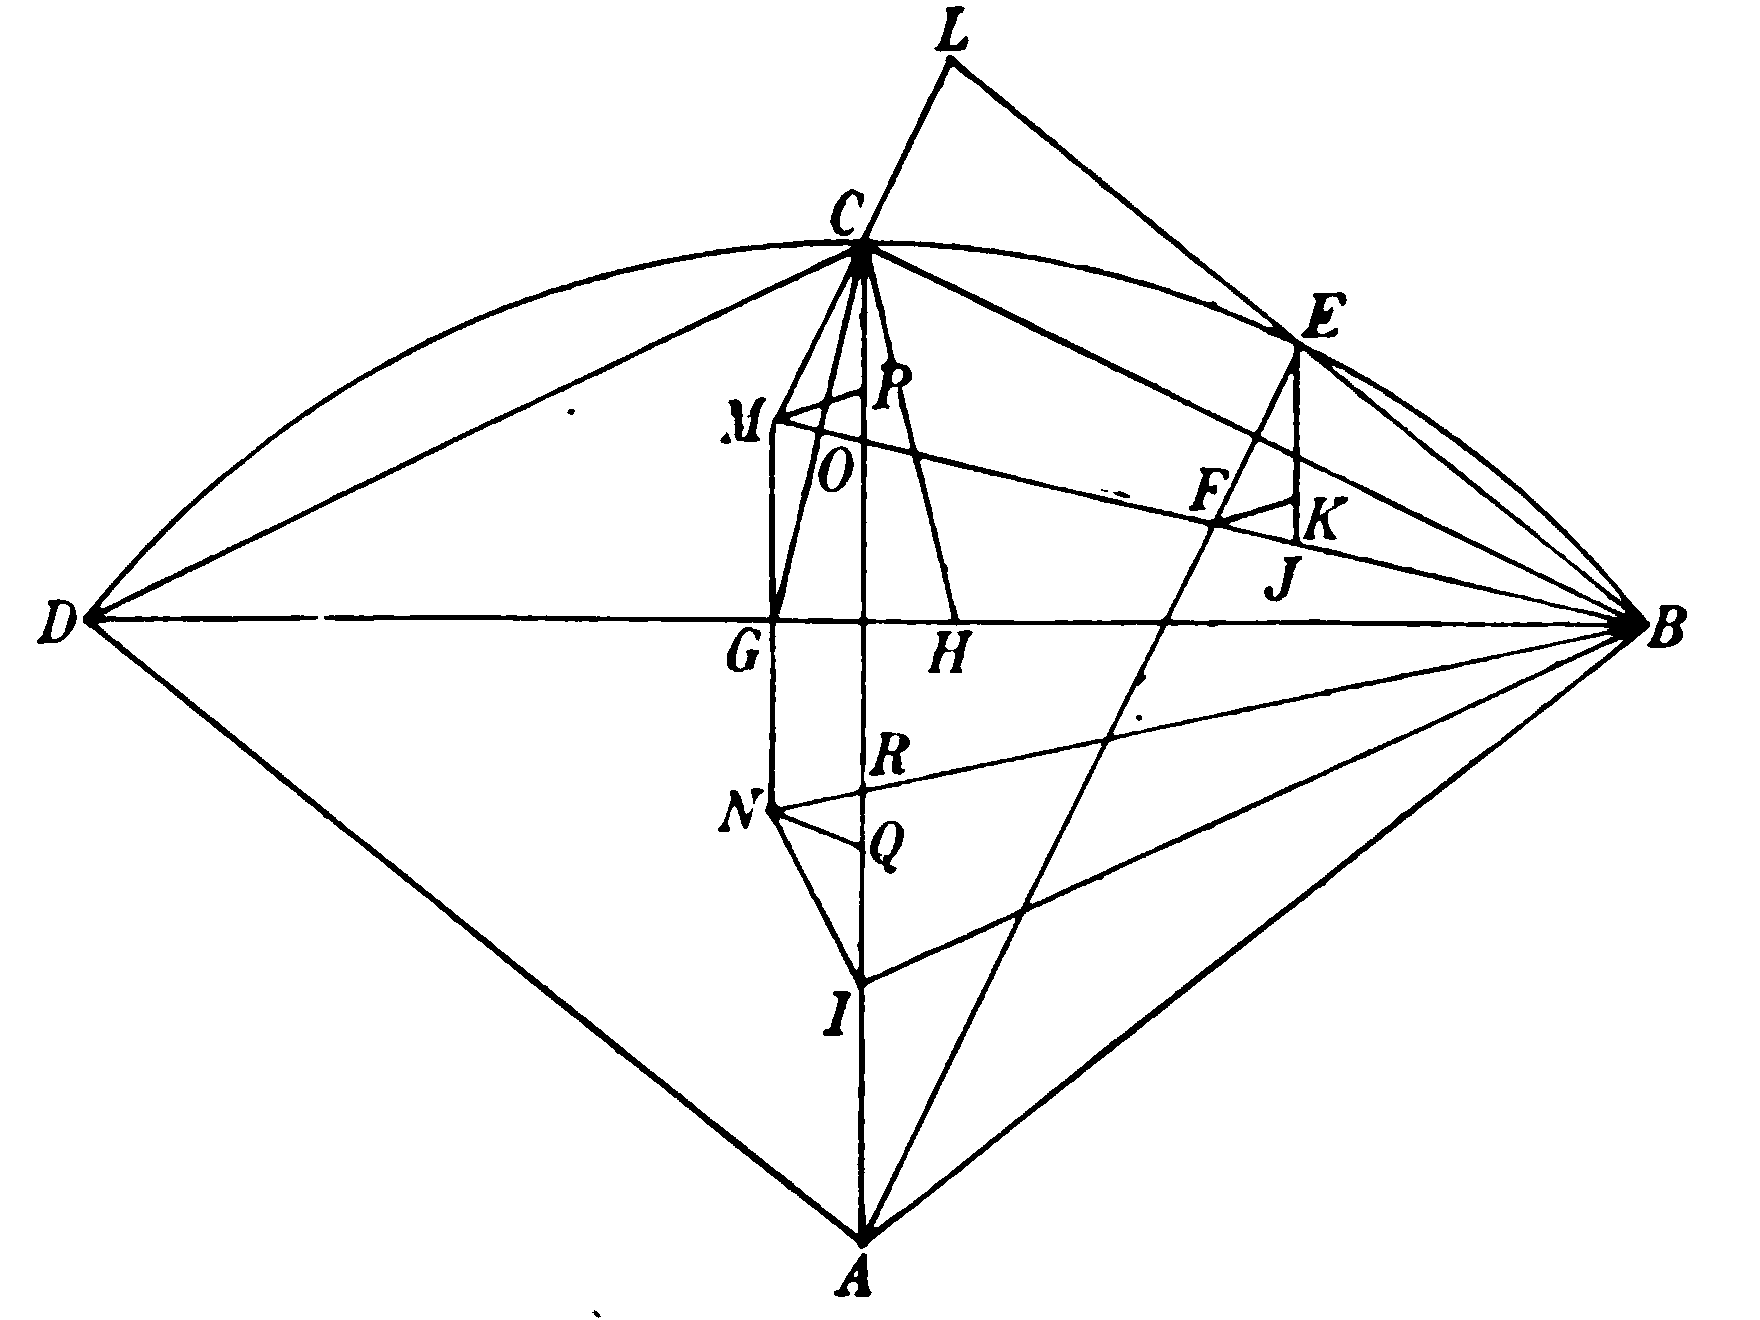
\includegraphics[width=0.56\linewidth]{pdf159-ming-chord-geometry.png}
\end{center}

In 1875 Tso Ch'ien's \emph{Chui-shu Shih-ming}, which was a commen-
\scanfooter

\scanpage{0160}{Chapter 21, printed page 146}
tary on Ming's book, was published as one volume of the \emph{Pai-fu-t'ang Collections}. If we don't know how much was due to Ming's original considerations and how much to Tso's additions, yet the outlines of the process employed were certainly taken from the original treatise. We shall therefore see about the procedures followed in the book. In the first place to express the chord of a segment of a circle in terms of its arc, the chord is expressed in terms of the chords of the 2nd, 3rd, \ldots{} parts of the given arc. In the figure let the radius of the circle be unity. In the segment $BCD$, whose centre is $A$, let $C$ be the middle of the arc, and let $E$ be the middle of the arc $BC$. Construct $BF=BE$, such that the point $F$ lies on the line $AE$. On $BD$ take $BG=BC$ and $DH=DC$. Then writing $BC=BG=a$ we have $BD=2a-GH$. Draw $EJ=EF$ and $FK=FJ$. Produce $BE$ and $BF$, and take $BL=2\cdot BE$ and $BM=2\cdot BF$. Join $LM$, which evidently passes through the point $C$. Turn the triangle $BML$ around the side $BM$ as axis. The point $C$ falls then on $G$, and let $N$ be the point upon which $L$ falls. If the triangle $NGB$ be turned again about $NB$ as axis, the point $G$ will fall on a point on $CA$. Call it $I$. Then evidently $BI=BC$. Again let $O$ be the point where $BM$ cuts $CA$, and construct $MP=MO$. Similarly draw $NQ=NR$ $R$ being the intersection of $BN$ with $CA$. After such a construction is tried, it is indicated that the triangles $ABE$, $BEF$, $FJK$, $BLM$, $CMO$, $MOP$, $CGH$ are all similar; and that the two triangles $CMO$ and $EFJ$ are congruent. We have therefore
\[
AB:BE=BE:EF,\qquad AB:EF=BC:GH,
\]
or,
\[
1:BE=BE:EF\quad\text{or}\quad EF=BE^2,
\qquad 1:BE^2=a:GH,
\]
whence follows $GH=a\cdot BE^2$, and hence we have $BD=2a-a\cdot BE^2$.

Carrying considerations upon this basis, in the end the following expression is obtained:
\[
BD=2a-\frac{a^3}{4}-\frac{a^5}{4^3}-\frac{2a^7}{4^5}-\frac{5a^9}{4^7}-\frac{14a^{11}}{4^9}-\cdots.
\]

\begin{center}
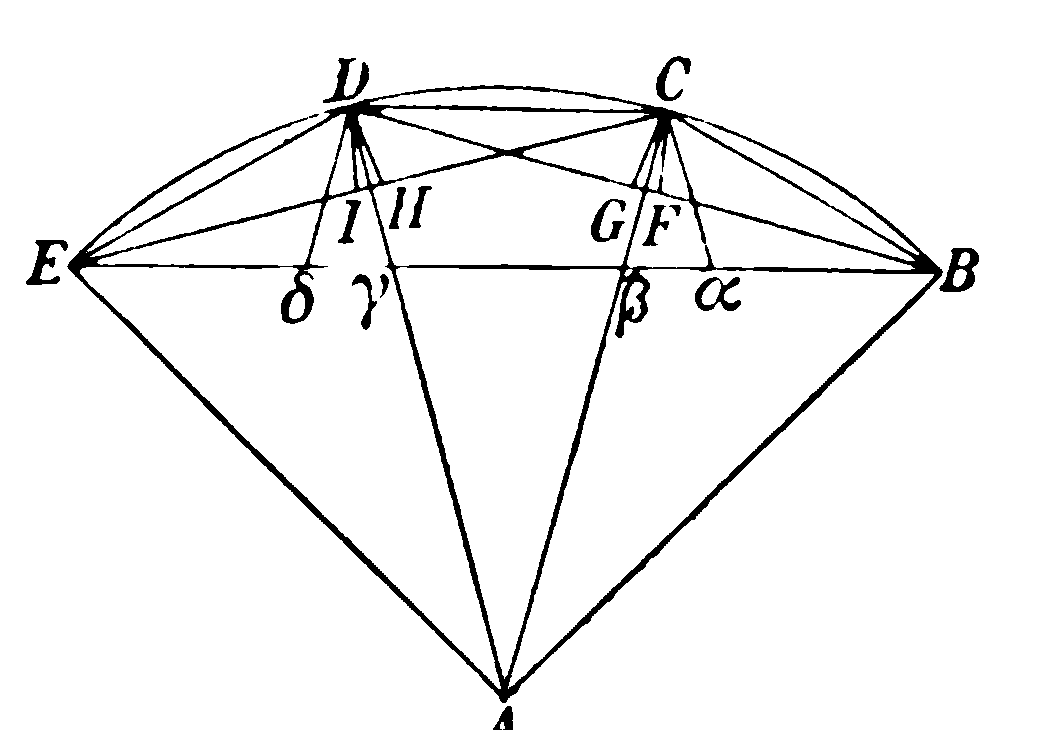
\includegraphics[width=0.38\linewidth]{pdf160-third-part-chord-diagram.png}
\end{center}

Next denoting the chord of a third part of an arc by $a$, in order to find the chord of the whole arc a figure is described as annexed. Here $BG$, $EH$ are constructed $=BC$, and $B\delta=E\alpha=BD$, and $\triangle C\alpha\beta\equiv\triangle D\delta\gamma\sim\triangle B\delta D$, and the like. We have then
\scanfooter

\scanpage{0161}{Chapter 21, printed page 147}
\[
AB:BC=BC:CG=CG:GF,\qquad BC:FG=BD:\delta\gamma,
\]
\[
2\cdot BD=BE+\delta\alpha\quad\text{or}\quad 2\cdot BD-\delta\gamma=BE+BC,
\]
\[
\therefore\quad 2\cdot BD-\delta\gamma-BC=BE.
\]
Proceeding hereupon, in the end the expression, $BE=3a-\frac{4a^3}{4}$, will be obtained.

When we denote by $a$ the chord of a fourth part of a given arc, whose chord is required to be expressed by means of $a$, we shall have in like way
\[
(\mathrm{chord})=4a-\frac{10a^3}{4}+\frac{14a^5}{4^3}-\frac{12a^7}{4^5}+\cdots.
\]
A similar treatment will lead, when we take $a$ for the chords of the 10th, 100th, 1000th, and 10000th part of a given arc, to the expressions for the chord of the arc as follows:
\[
10a-\frac{165}{4}a^3+\frac{3003}{4^3}a^5-\frac{21450}{4^5}a^7+\cdots,
\]
\[
100a-\frac{166\,650}{4}a^3+\frac{3330\,00030}{4^3}a^5-\frac{31\,63500\,28500}{4^5}a^7+\cdots,
\]
\[
1000a-\frac{1666\,66500}{4}a^3+\frac{3333\,30000\,00300}{4^3}a^5-\cdots,
\]
\[
10000a-\frac{16\,66666\,65000}{4}a^3+\frac{3333\,33300\,00000\,03000}{4^3}a^5-\cdots.
\]
If we take the coefficients of $a^3$ in the last three of these expressions as divisors and divide with them respectively the quantities $100^3$, $1000^3$, $10000^3$, we get
\[
24\cdot0024\ldots,
\qquad 24\cdot00002\,4\ldots,
\qquad 24\cdot00000\,024\ldots.
\]
Hence the members of the series with these numbers as the first terms will be seen to approach more and more to the value 24. We see therefore that, when the arc is taken as the first term, the second term in the expression of the chord is to be taken as $=-\frac1{24}(\arcop)^3$.

In like way we may calculate with the coefficients of $a^5$ and the numbers $100^5$, $1000^5$, $10000^5$, and find the ratios with the preceding terms, when we get
\[
80\cdot07\ldots,
\qquad 80\cdot0007\ldots,
\qquad 80\cdot00000\,7\ldots,
\]
and we conclude that the limiting value of the series will approach to 80. Hence the third term of our series is to be taken
\[
=\frac1{24\times80}(\arcop)^5.
\]
\scanfooter

\scanpage{0162}{Chapter 21, printed page 148}
In like way the 4th term will be found $=\frac1{24\cdot80\cdot168}(\arcop)^7$, and so on. But the numbers $24$, $80$, $168$, \ldots{} are of the forms
\[
24=4(2\cdot3),\qquad 80=4(4\cdot5),\qquad 168=4(6\cdot7),\ldots,
\]
so that finally we obtain the formula for the chord in the form:
\[
(\mathrm{chord})=(\arcop)-\frac{(\arcop)^3}{4\times3!}+\frac{(\arcop)^5}{4^2\times5!}-\frac{(\arcop)^7}{4^3\times7!}+\cdots.
\]
Here it will be observed that the imperfect induction is skillfully applied. This point highly resembles the development of the Japanese \emph{yenri} theory, as will be seen in a subsequent chapter.

Next to find the arc ($a$) in terms of its chord ($c$), a process of reversion is applied to the series just obtained. Writing the radius $=m_1$, and the series for $c=m_2$, and forming the continued proportion
\[
m_1:m_2=m_2:m_3=m_3:m_4=m_4:m_5=\cdots,
\]
we get on calculation
\[
m_2=a-\frac1{4\times3!}a^3+\frac1{4^2\times5!}a^5-\frac1{4^3\times7!}a^7+\cdots,
\]
\[
m_4=a^3-\frac3{4!}a^5+\cdots,
\qquad
m_6=a^5-\frac5{4\times3!}a^7+\cdots,
\]
etc., whence follows by successive additions
\[
m_2+\frac{m_4}{3!\cdot4}=a+0-\frac{9a^5}{5!\cdot4^2}+\cdots,
\]
\[
m_2+\frac{m_4}{3!\cdot4}+\frac{9m_6}{5!\cdot4^2}=a+0+0-\frac{228a^7}{7!\cdot4^3}+\cdots,
\]
\[
m_2+\frac{m_4}{3!\cdot4}+\frac{9m_6}{5!\cdot4^2}+\frac{228m_8}{7!\cdot4^3}=a+0+0+0-\cdots,\quad\mathrm{etc.}
\]
At the end of the operation, therefore, we shall have
\[
a=m_2+\frac1{3!\cdot4}m_4+\frac9{5!\cdot4^2}m_6+\frac{228}{7!\cdot4^3}m_8+\cdots,
\]
or
\[
a=c+\frac1{3!\cdot4}c^3+\frac9{5!\cdot4^2}c^5+\frac{228}{7!\cdot4^3}c^7+\cdots.
\]
Of Tu Tê-mei's or Jartoux's formulae, the expansions of $\sin x$ and $\versin x$, or $\cos x$, for we have $\cos x=1-\versin x$, were first obtained in Europe by James Gregory (1638--1675) in his \emph{Vera Circuli et Hyperbolae Quadratura} of 1667. The expansion of $\arcop\sin x$
\scanfooter

\scanpage{0163}{Chapter 21, printed page 149}
was given by Sir Isaac Newton in his writings dated 1676; and in the expansion he applied the reversion of series. Thus Jartoux who came to China some years later than the invention of these series, might have been acquainted with these results arrived at by the English mathematicians, although he was a Frenchman. The reversion of series employed by Ming An-t'u in his book as we have described may also have been learned from a European source through Jartoux's hand. We are not however certain whether Newton's way was the same as Ming's. The two await comparison in detail.

Tu Tê-mei's formula for the square of an arc is the same as was given by the Japanese Takebe Kenkō in 1722. But his way of analysis was utterly different from that employed by Ming in China. In the Western World the series was published by J. de Stainvilles in his \emph{Melanges d'Analyse Algebrique et de Géometrie}, p. 460, Paris, 1815. It was given however some time previously by Leonhard Euler in a letter to Johann Bernoulli of December 10th, 1737, a letter that was printed for the first time by G. Eneström in 1904.\footnote{P. Harzer, \emph{Die exacten Wissenschaften im alten Japan}, \emph{Jahresbericht der D. M. V.}, Bd. 14, pp. 318--319. The said letter of Euler is given in the \emph{Bibliotheca Mathematica}, 3. Folge, V, p. 270.} Besides these instances we must own we are utterly ignorant of the existence of the series in Europe in the 18th century or previously.

If Tu Tê-mei or Pierre Jartoux had actually possessed the series, he may have obtained it himself. In that case we must admit he was a talented mathematician. Had he learned all his nine formulae from his predecessors, we must equally admire his profoundness of knowledge, and our admiration grows the more when we reflect that he had been no professional mathematician. At any rate the Chinese mathematics was largely enriched by his introduction of these formulae. Had he taught of the analysis leading to these results, or had Mei Ku-ch'êng recorded what had been taught by him, the Chinese would undoubtedly have gained much more.

If the series was not in actuality taught by Tu Tê-mei and if it was first established by Ming An-t'u, as T. Hayashi conjectures, then Ming's merit is highly deserving in the mathematical history of the Chinese. It is certain that his persevering labours have contributed considerably to arouse the interest of later mathematicians. In any case he was the first instance of the Chinese entering into the analytical study of the subject. Ming was crowned with the success in his studies nearly half a century after Takebe had succeeded in the estab-
\scanfooter

\scanpage{0164}{Chapter 21, printed page 150}
lishment of the same series in Japan, but the modes of analysis followed by the two scholars were entirely. different.

Fang Ching-fu, who was a contemporary of Yüan Yüan, and who therefore belonged to the end of the 18th century or the beginning of the 19th century was also interested in the expansions in infinite series. According to Lo Shih-lin,\footnote{Lo's ``Supplements to Biographical Collections'', Book 48.} Fang obtained Tu Tê-mei's nine formulae and studied them. If it was in a time before the publication of Ming An-t'u's book,\footnote{Ming's work was first printed in 1840.} Fang's results were seen on examination to agree with those of the other.

Half a century after Ming there appeared Tun Yu-ch'êng (1791--1823). His work \emph{Ko-yüan Lien-pi-li T'u-chieh}, consisting of three books, concerned the same line of studies. It was an old manuscript containing Tu Tê-mei's nine formulae that instigated him to work. The old manuscript was procured by him in 1819 from Chu Hung. Tun supplied explanations or analysis to the derivation of Tu's formulae, and added four others. After his book had been complete, he obtained Ming's book, but, as he saw, the procedures followed by the two mathematicians were not necessarily the same.\footnote{Lo's ``Supplements'', Book 51, and Chu's ``Third Part'', Book 2.} The four formulae obtained by Tun are as follows:\footnote{Hsü Yu-t'ing's \emph{T'sê-yüan Mi-lu}, Book 3.}
\[
\begin{aligned}
b={}&\frac{a}{n^2}+\frac{(n^2-1)T_1\cdot2T_1}{r\times3\cdot4}
+\frac{(4n^2-1)T_2\cdot2T_1}{r\times5\cdot6}
+\frac{(9n^2-1)T_3\cdot2T_1}{r\times7\cdot8}+\cdots,\\
a={}&n^2b-\frac{(n^2-1)T_1\cdot2b}{r\times3\cdot4}
+\frac{(n^2-4)T_2\cdot2b}{r\times5\cdot6}
-\frac{(n^2-9)T_3\cdot2b}{r\times7\cdot8}+\cdots,\\
b'={}&\frac{a'}n+\frac{(n^2-1)T_3\cdot T_1^2}{r^2\times2\cdot3}
+\frac{(9n^2-1)T_2\cdot T_1^2}{r^2\times4\cdot5}
+\frac{(25n^2-1)T_3\cdot T_1^2}{r^2\times6\cdot7}+\cdots,\\
a'={}&nb-\frac{(n^2-1)T_1b^2}{r^2\times2\cdot3}
+\frac{(n^2-9)T_2b^2}{r^2\times4\cdot5}
-\frac{(n^2-25)T_3b^2}{r^2\times6\cdot7}+\cdots,
\end{aligned}
\]
where $a$ is the chord of an arc (the half of which we write $x$), $b$ that of the $n$th part of this arc, $a'=\sin x$, $b'=\sin\frac{x}{n}$, $r=$ the radius, and $T_1$, $T_2$, \ldots{} are the 1st, 2nd, \ldots{} terms.

The Chinese did not attempt to rectify the ellipse until at the beginning of the 19th century. Chu Hung was certainly the first person who took up the problem in China. He obtained the degree of \emph{chin-shih} in 1802 and remained in service until he retired in 1830.
\scanfooter

\scanpage{0165}{Chapter 21, printed page 151}
He thenceforth lived some years in Peking. Chu enjoyed the friendship of Tun and other mathematicians, with whom their subjects were advantageously discussed.\footnote{Chu's ``Third Part of Biographical Collections'', Book 2.} Chu Hung knew that an oblique section of a circular cylinder would give an ellipse, and he considered consequently that the calculations about the ellipse could be effected by aid of a right triangle. Tun Yu-ch'êng tried thereupon a graphical explanation. He thought, if the circle is like a square, then the ellipse is like a rectangle. In the ellipse there occur such quantities as the major axis, the minor axis, the perimeter, the area, etc. If of these we know any two,. the others may be found therefrom. According to Lo Shih-lin,\footnote{Lo's ``Supplements'', Book 51.} Tun's treatment of this problem, it seems, was effected in the same manner as the length of a vine winding the trunk of a tree had been calculated in the \emph{Chiu-chang} or ``Nine Sections''. The formula he obtained was
\[
(\mathrm{half\ perimeter})=\sqrt{(a^2-b^2)+\left(\frac12b\pi\right)^2},
\]
where $a$ and $b$ are the lengths of the major and minor diameters. Of its incorrectness Lo was already aware. Tun's studies extended besides these over the domain of the progressions of higher orders, of spherical trigonometry, and of calendrical subjects. If Wang Lai had previously studied about the progression whose $n$th term is of the fourth degree in $n$, yet it remained for Tun to consider progressions with terms that are to be expressed by higher algebraical expressions.\footnote{Ibid.}

About contemporary with Tun, another scholar became noted also for his studies of the analytical considerations of the circle. He was Hsiang Ming-ta (1795--1850). He studied spherical trigonometry, and then he took to himself the subject of finding the length of an elliptic arc. He then came to follow Tun's results about the infinite expansions concerning the circle, but he did not live to see his work \emph{Hsiao-su Yüan-shih} completed. It was subsequently supplemented by Tai Hsü in fulfilment of the author's request. Thus the 7th book of the treatise was written by Tai. In the 6th book Hsiang resorted to infinite series to express the elliptic perimeter and he also resorted to the same to solve equations. In 1860 Hsü Yu-t'ing was about to publish the work, the wood-blocks having been almost wholly prepared, when he fell in battle. Consequently the publication was retarded
\scanfooter

\scanpage{0166}{Chapter 21, printed page 152}
and the book was lost altogether, never again appearing in the mathematical circle.\footnote{Chu's ``Third Part of Biographical Collections''.}

Hsiang's contemporary Tai Hsü (1805--1860) wrote the \emph{Wai-chieh Mi-lu}, consisting of four books. About the same time, Li Shan-lan wrote the \emph{Shih-shih Mong-pi}, and Hsü Yu-t'ing wrote the \emph{T'sê-yüan Mi-lu} and the \emph{Ko-yüan Chui-shu}, etc. These works all concern the same or allied subjects. Hsü's \emph{T'sê-yüan Mi-lu}\footnote{T'ing Ch'u-chung's edition of Hsü's work.} or ``Accurate Formulae of the Circle-Measurement'' contains among others the following formulae,
\[
p^2=9d^2\left(1+\frac{1^2}{3\cdot4}+\frac{1^2\cdot2^2}{3\cdot4\cdot5\cdot6}+\frac{1^2\cdot2^2\cdot3^2}{3\cdot4\cdot5\cdot6\cdot7\cdot8}+\cdots\right),
\]
\[
p^3=54q\left(1+\frac{1^2}{3\cdot4}+\frac{1^2\cdot2^2}{3\cdot4\cdot5\cdot6}+\frac{1^2\cdot2^2\cdot3^2}{3\cdot4\cdot5\cdot6\cdot7\cdot8}+\cdots\right),
\]
where $p$ is the circumference of a circle of diameter $d$, and $q$ the volume of a sphere of equal diameter. The volume of an ellipsoid of revolution, elliptic cylinder, elliptic cone and its frustum are given respectively equal to
\[
\frac{a^2b}{2},\qquad \frac34abh,\qquad \frac14abh,\qquad
\frac18h\{(2a+a')b+(2a'+a)b'\},
\]
which are multiplied by
\[
\pi=1+\frac{1^2}{3!\cdot4}+\frac{1^2\cdot3^2}{5!\cdot4^2}+\frac{1^2\cdot3^2\cdot5^2}{7!\cdot4^3}+\cdots,
\]
where $a$ and $b$ denote the major and minor diameters and where the meanings of $a'$, $b'$ and $h$ are obvious.

Hsü Yu-t'ing was born 1801 at Wu-chêng and took the degree of \emph{chin-shih} in 1829. During the Taiping Rebellion he was the military governor of Chiang-su. In 1860 the imperial army was defeated at Ching-nan and the viceroy fled for life. The rebel troups soon pressed on in inundations to Su Chou. Hsü the Governor conducted the defence valiantly at the head of his troops. But the garrison, not being more than 4000 men, soon gave way. Hsü fell stabbed by a sword, and his whole family were all killed. Hsü was noted for his honest policy and eagerness, observant to duty, while he lived. Some of his works were published by himself in his life-time, but others that remained unpublished were mostly lost at the time of his death Hsü was accustomed in the early part of his life to write down only the results he had obtained, leaving the analysis employed without
\scanfooter

\scanpage{0167}{Chapter 21, printed page 153}
description. Being advised however that it would be more beneficial to after ages, if he should try to give the accounts of his detailed studies, he had desired to follow the advice, but he did not live long to realise the attempt, for he was too busy in his after-life to have leisure for writings.\footnote{Chu's ``Third Part of Biographical Collections'', Book 4.}

In the appendix to Hsü's ``Measurement of the Sphere'' we find some formulae for the perimeter of the ellipse. We have already given the formula obtained by Tun. After Tun's time, Hsiang Ming-ta tried the rectification by measuring the circumference of the circle, described on the major axis as diameter, and the difference of the perimeters. Tai Hsü did the same applying to the measurement of the circle on the minor axis as diameter and the difference of the perimeters. Hsü Yu-t'ing then obtained another formula that was more satisfactory, as he says.\footnote{Hsü's ``Measurement of the Sphere'', appendix. Ting's reprint.} Here we give from Hsü's work the formulae of Hsiang and Tai, which are as follows: If we write
\[
\begin{aligned}
K={}&\frac{m}{a}+\frac{1^2\cdot3}{2^2}\frac{m^2}{a^3}
+\frac{1^2\cdot3^2\cdot5}{2^2\cdot3^2}\frac{m^3}{a^5}
+\frac{1^2\cdot3^2\cdot5^2\cdot7}{2^2\cdot3^2\cdot4^2}\frac{m^4}{a^7}+\cdots,\\
K'={}&\frac{m}{b}-\frac{1^2\cdot3}{2^2}\frac{m^2}{b^3}
-\frac{1^2\cdot3^2\cdot5}{2^2\cdot3^2}\frac{m^3}{b^5}
-\frac{1^2\cdot3^2\cdot5^2\cdot7}{2^2\cdot3^2\cdot4^2}\frac{m^4}{b^7}-\cdots,
\end{aligned}
\]
where $a$ and $b$ are the major and minor diameters and where $m=\frac14(a^2-b^2)$, then the elliptic perimeter will be expressed by $K\pi a$ and $K'\pi b$. Hsü's own formula was expressed by finding the circumference of a circle isoperimetric with the ellipse. It is our great regret that we have no material for describing the processes or analysis by which these formulae were calculated.

We shall try in the following lines to say something of Hsü's process of calculating the altitude of a circular segment in terms of the chord.\footnote{Hsü's \emph{Ko-yüan Chui-shu} or the ``Analysis of Circle-Measurement'', Book 2, commented by Wu Chia-shan and supplemented by Tso Ch'ien, Published by Ting, 1874.} The formula we have to explain is $\versin x=T_1+T_2+T_3+\cdots$, where the successive terms are of the forms
\[
T_1=\frac{\sin^2x}{d},\qquad
T_2=\frac{T_1^2}{d},\qquad
T_3=\frac{(2T_1+T_2)T_2}{d},\qquad
T_4=\frac{[2(T_1+T_2)+T_3]T_3}{d},\ldots.
\]
For the purpose of deriving this expression, the considerations are started from a figure as annexed. The rectangle is so constructed
\scanfooter

\scanpage{0168}{Chapter 21, printed page 154}
that $EK=$ the sagitta, $KA=$ the supplemental sagitta or the difference of the diameter and the given sagitta, while $KC$ is equal to $KE$.

\begin{center}
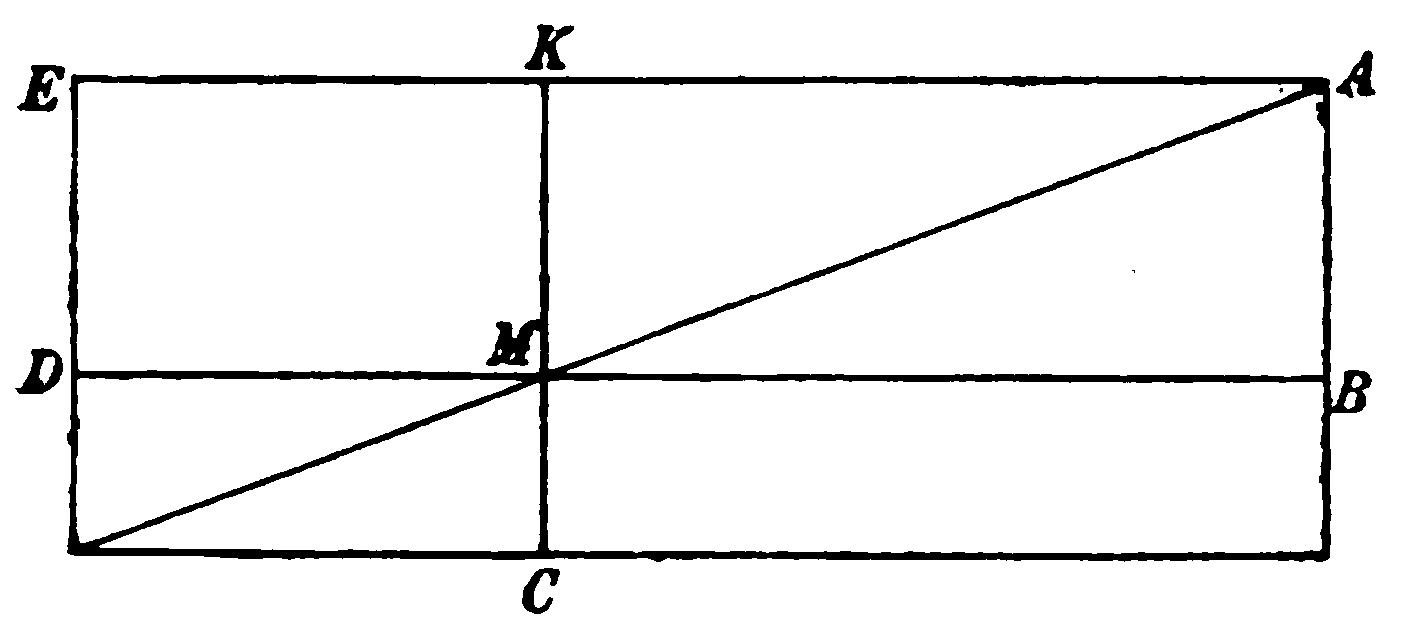
\includegraphics[width=0.50\linewidth]{pdf168-rectangle-derivation-1.png}
\end{center}

Here the rectangle $AC$ is $=$ the product of the sagitta and the supplemental sagitta, namely, equal to $\sin^2x$. But $\rectsym AC=\rectsym AD$, $\therefore\ \rectsym AD=\sin^2x$, so that we get, after the division by the diameter $d$, the length of $ED$, which we write $T_1$. Thus $T_1=\sin^2x/d$.

Next constructing the figure as shown here, we have $\rectsym KN=\rectsym NH=\rectsym BG$. But $\rectsym KN=T_1T_1$, and so we write $T_1T_1/d=DG=T_2$.

\begin{center}
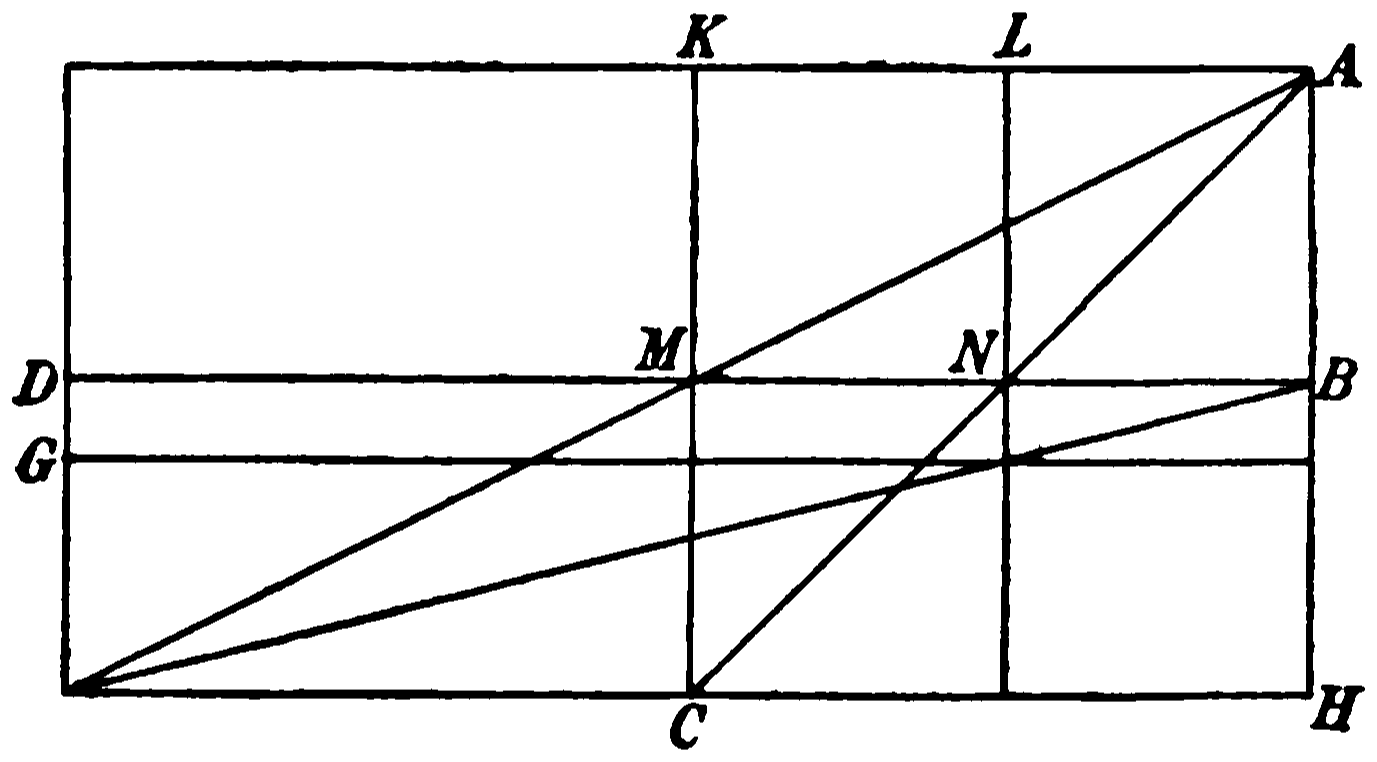
\includegraphics[width=0.52\linewidth]{pdf168-rectangle-derivation-2.png}
\end{center}

Next drawing the figure as annexed, where the ruled area is intended to become a square, we have $\rectsym LN'=(T_1+T_2)T_2=\rectsym DG'$, where $G'$ is taken such that $MD'=N'H'$. We have also $\rectsym MM'=T_2T_1$, $\therefore\ \rectsym DG'+\rectsym MM'=(2T_1+T_2)T_2$. Again $\rectsym DM'=\rectsym M'H$, and so $(2T_1+T_2)T_2=\rectsym N'H=\rectsym B'G''$, $\therefore\ T_3=\frac{(2T_1+T_2)T_2}{d}=GG''$.

\begin{center}
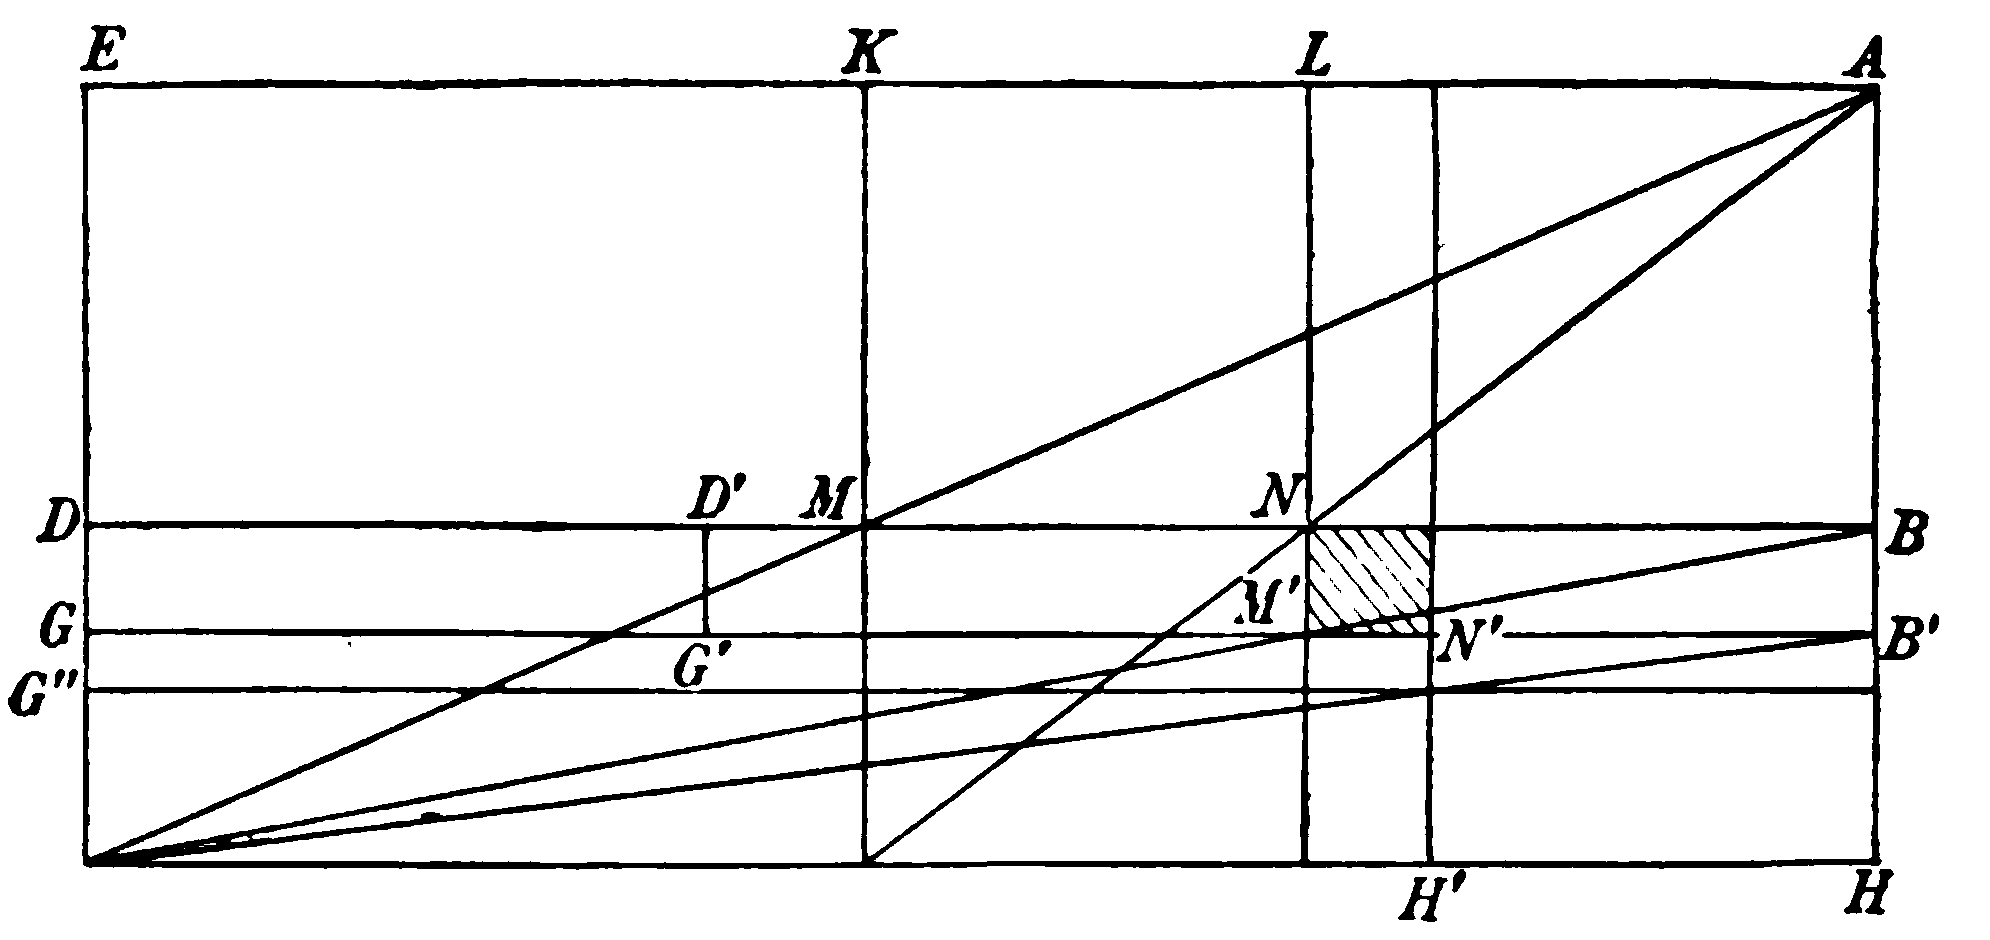
\includegraphics[width=0.58\linewidth]{pdf168-rectangle-derivation-3.png}
\end{center}

In this way the expansion as we have mentioned above may be obtained. But Hsü goes further to transform it. Thus it will be seen that the following proportions exist:
\[
\begin{array}{rcl}
(1)&d:\sin x&=\sin x:T_1,\\
(2)&d:T_1&=T_1:T_2,\\
(3)&d:T_2&=2T_1+T_2:T_3,\\
(4)&d:T_3&=2(T_1+T_2)+T_3:T_4,\ldots.
\end{array}
\]
\scanfooter

\scanpage{0169}{Chapter 21 conclusion, printed page 155}
Now write $m_1=r$ or radius, $m_2=\sin x$, and form the continued proportions:
\[
m_1:m_2=m_2:m_3=m_3:m_4=m_4:m_5=\cdots,
\]
which means to take $m_k=\sin^{k-1}x/r^{k-2}$. Prepared with this notation, we have from the proportions given above,\footnote{The proportion is represented in the work in the form annexed. Here the terms are to be counted from right to left.
\[
\begin{array}{|c|c|c|c|}
\hline
d&c&b&a\\
\hline
\end{array}
\]}
\[
(1)\quad 2m_1:m_2=m_2:\frac{m_3}{2},
\qquad
(2)\quad 2m_1:\frac{m_3}{2}=\frac{m_3}{2}:\frac{m_5}{2\cdot4}.
\]
The formula (3) is considered divided into two proportions\footnote{These proportions are originally designated as annexed.
\[
\begin{array}{|c|c|c|c|}
\hline
\dfrac{2m_7}{2\cdot4^2}&\dfrac{2m_3}{2}&\dfrac{m_5}{2\cdot4}&2m_1\\
\hline
\dfrac{m_9}{2\cdot4^3}&\dfrac{m_5}{2\cdot4}&\dfrac{m_5}{2\cdot4}&2m_1\\
\hline
\end{array}
\]}
\[
2m_1:\frac{m_5}{2\cdot4}=\frac{2m_3}{2}:\frac{2m_7}{2\cdot4^2}
\quad\text{and}\quad
2m_1:\frac{m_5}{2\cdot4}=\frac{m_5}{2\cdot4}:\frac{m_9}{2\cdot4^3},
\]
and the fourth proportionals are added together to give $T_3$, which is
\[
=\frac{2m_7}{2\cdot4^2}+\frac{m_9}{2\cdot4^3}.
\]
In like way $T_4$ and $T_5$ will be obtained
\[
T_4=\frac{4m_9}{2\cdot4^3}+\frac{6m_{11}}{2\cdot4^4},
\qquad
T_5=\frac{8m_{11}}{2\cdot4^4},
\]
where $m_{13}$ and further terms are neglected. Adding these results together we have $T_1+T_2+T_3+\cdots$ equal to
\[
\frac{m_3}{2}+\frac{m_5}{2\cdot4}+\frac{2m_7}{2\cdot4^2}+\frac{5m_9}{2\cdot4^3}+\frac{14m_{11}}{2\cdot4^4}+\cdots,
\]
which is the same thing as to take the formula:
\[
\mathop{\mathrm{ver\,sin}}x
=\frac12\frac{\sin^2x}{r}
+\frac1{2\cdot4}\frac{\sin^4x}{r^3}
+\frac2{2\cdot4^2}\frac{\sin^6x}{r^5}
+\frac5{2\cdot4^3}\frac{\sin^8x}{r^7}+\cdots.
\]
\scanfooter


\scanpage{0170}{Part II and Chapter 22 opening, printed page 156}
\begin{center}
PART II.\\[1mm]
THE JAPANESE MATHEMATICS.\\[3mm]
CHAPTER 22.\\[1mm]
A GENERAL VIEW OF THE JAPANESE MATHEMATICS.
\end{center}
\phantomsection\addcontentsline{toc}{section}{Part II. The Japanese Mathematics}
\phantomsection\addcontentsline{toc}{subsection}{Chapter 22. A General View of the Japanese Mathematics}

Of the mathematical knowledge possessed by the Japanese in the oldest times we know practically nothing. After the introduction of Buddhism through Korea in the 6th century, something of the Chinese mathematics was brought to Japan and studied for some time by native scholars. But their knowledge must have been exceedingly limited, for they did not ever rise to the point of carrying on their work independently. Blind adherence to Chinese masters was all that they could do. Even such a menial state did not continue very long, for with the loosening of political regulations learning too shared the same fate, gradually degenerating until at last practically nothing remained.

It was after a reintroduction of the Chinese mathematics that the Japanese became really observant of mathematical studies. After the long duration of the dark ages the 17th century at last saw the science taken up into favour for a second time, when there appeared various scholars, in whose hands the Japanese mathematics properly so called was destined to dawn and flourish for more than two centuries that followed.

The first Japanese mathematician noted in history was Mōri Kambei who lived at the beginning of the 17th century. He is sometimes referred to as having traveled to China, but the story is not certainly authentic.

The Chinese abacus \emph{suan-pan}, which the Japanese call \emph{soroban}, has extensively been used in Japan since Mōri's days. As is usually believed, it was first brought by him from China, but its introduction seems to be more ancient. In any case, however, Mōri was a dexterous hand in the art of manipulating the instrument. He taught the \emph{soroban} arithmetic at Kyōto, when a multitude of pupils crowded around him. In popularizing the abacus Mōri was certainly no little instrumental. Mōri published, it is said, a treatise on the use of the \emph{soroban}, but it has since been lost.
\scanfooter

\scanpage{0171}{Chapter 22, printed page 157}
Of Mōri's numerous pupils there were three, who distinguished themselves specially. These three were Yoshida Kōyū, Imamura Chishō and Takahara Kisshū. The \emph{Sanshi}, meaning ``Three Honorable Mathematicians or Scholars'', was the appelation respectfully given them by their contemporaries.

Yoshida's \emph{Jinkōki} of 1627 was a successful publication. After its appearance the \emph{soroban} arithmetic experienced a rapid progress. The book was destined to earn such a popularity that it went through various editions even in the life-time of its illustrious author. Sometimes booksellers made reprints of it without the author's knowledge or permission. In after ages there were published tens of treatises with the same title, to which some prefixes were added.

Yoshida's work was followed by various other publications, which were, like it, mostly based on the contents of the Chinese Ch'êng Tai-wei's \emph{Suan-fa T'ung-tsung} of 1593. This Chinese master was reprinted in Japan in 1675.

The first half of the 17th century was a period for the Japanese mathematics, when the arithmetic practised on the \emph{soroban} was becoming popularised in every part of the country. But now another stimulation to the progress of the science appeared. It was the introduction of another Chinese treatise, Chu Shih-chieh's \emph{Suan-hsiao Chi-mêng} of 1299. Of Chu's works mention has been made in chapter 14. The said treatise had been long missing in China until it was restored by the discovery of a Korean edition of 1660 and was reprinted by Lo Shih-lin in 1839. Even the learned Yüan Yüan was not able to find the book at the time of his historical studies.\footnote{His ``Biographical Collections'' was complete in 1799.} This work, although missing in China, had the happy destiny of being found in Japan, perhaps introduced from Korea, where it was once reprinted in 1660. But the Japanese knew it from before that date; for the first Japanese edition was given in 1658. It was widely studied by Japanese mathematicians of the 17th century and supplied them with the rudiments of the instrumental algebra that was carried on by means of the calculating pieces or \emph{sangi}, as they were now called in Japan. This was the so-called \emph{t'ien-yuen-shu} or the Japanese \emph{tengen jutsu}, which literally means ``the celestial element method''.

The \emph{sangi} or calculating pieces were no new makeshifts. Their use in China we have already referred to. When the Chinese mathematics was introduced for the first time from Korea to Japan, these
\scanfooter

\scanpage{0172}{Chapter 22, printed page 158}
pieces were also undoubtedly brought over, and they have remained in use ever since. But with the popularising of the \emph{soroban} the calculating pieces were fast giving way, for they are far more cumbrous and non-practical, when compared to the new sort of abacus. If the algebra of the celestial element method had not come to be studied, these pieces would certainly have altogether sunk into oblivion ere long. It was not however the case. While the \emph{soroban} was suitable for the practice of daily-life, the calculating pieces served best for the discussion of complicated problems, being applicable to the solution of numerical equations of any degree. Thus it came about that the two sorts of abaci, the \emph{soroban} and the \emph{sangi}, had to flourish side by side. Both were practised during the whole era of the ascendency of the old Japanese school of mathematics.

Mathematical studies had been in continual progress since the appearance of Yoshida's \emph{Jinkō-ki} in 1627, but the introduction of the celestial element method contributed to considerably improve the scholars' knowledge, and it was not long afterwards that the Japanese began to enter upon independent work.

While the Chinese mathematicians of the 13th and 14th centuries studied the algebra of the celestial element, they all contented themselves with a single solution of an equation, whatever its degree might be; they did not come to discover the existence of more than one root in an equation. But the Japanese soon found that the roots of an equation are not necessarily restricted to a single one. Satō Seikō (1666) adopted various solutions to a problem that arise from the multiplicity of roots. Thereupon Sawaguchi Kazuyuki (1670) attacked the looseness of such a procedure, though he had admitted the existence of more than one solution under certain circumstances. He ascribed the origin of such solutions to the inappropriateness of the quantities constituting the data of the problems. He thus preferred to change some of the constants occurring in these data so as to yield a single solution.

Soon after the publication of the works of these scholars there appeared a great genius who is called the Japanese Newton. Seki Kōwa was his name. Seki was born in the same year in which Galileo died and Newton was born, namely in 1642. If Seki did not surpass Newton in his achievements, yet he was no inferior of the two. The same uplift Newton gave the mathematics of his country, Seki was also able to render for Japan. The Japanese mathematics properly so called had awaited his genius for its sound establishment. Nodoubt was Seki the father of Japanese mathematics.
\scanfooter

\scanpage{0173}{Chapter 22, printed page 159}
It is said, Seki wrote a great number of manuscript works in his life, but what now remain of the transcripts of these manuscripts are not very numerous. It is a great pity, we must confess, that nothing is known of works in his own hand-writing. But the few written works that are still preserved are sufficient to immortalise his memory. Who can deny his having been a mathematician of the first rank?

Seki wrote very much but printed little. He did not publish any of his works, except the single book entitled \emph{Hatsubi Sampō}, that appeared in 1674. Its appearance was however the occasion of bringing him the fame he deserved.

In a later edition of the \emph{Jinkōki} Yoshida published some mathematical questions at the end of the book and proposed to solve them for his successors. Isomura solved these problems in his \emph{Ketsugishō} of 1660 and published some other questions at the end of his work. These were in turn solved in some succeeding publications that were printed in a few years. In this way there arose the usage of proposing new questions and solving them in successive publications, a usage that continued for a century and a half. It was known as the usage of the \emph{idai shōtō}---the successive proposals and solutions. It had stimulated no little the progress of mathematical studies. The works of Satō (1666) and of Sawaguchi (1670), already referred to, were, with others, publications in this line. Sawaguchi proposed fifteen new questions, and it was Seki's work that answered them. One of Seki's solutions had led to an equation of the 1458th degree. It may be better imagined than described how tremendous such an equation should have been. Seki does not, it is true, give the equation itself, but mentions it expressly. A score of years afterwards Miyagi Seikō wrote the \emph{Wakan Sampō}, printed in 1695, in which he considered the same problem, when he gave the detailed analysis leading to the equation of the 1458th degree mentioned by Seki. The consideration of equations of wonderfully great degrees was not rare among the Japanese mathematicians of the 17th and 18th centuries. Sometimes equations whose degrees were 3000 or 4000 were taken into account. However great the degree might be, the Japanese solved them invariably by applying the celestial element method. In solving these tremendous equations the usual paper or wooden boards would be too insignificant for the arrangement of the \emph{sangi} pieces, and therefore, it is said, a certain mathematician prepared a \emph{sangi}-board ruling over the matts of his study or sitting room, whereupon he arranged the small pieces to
\scanfooter

\scanpage{0174}{Chapter 22, printed page 160}
solve equations. Perseverance and hard study were a part of the spirit that characterised Japanese mathematicians of old times.

The mathematical method Seki had used in writing his published work was that he called the \emph{yendan jutsu}, which literally means ``the method of explanations or of analysis''. It was an extension of the celestial element algebra of the Chinese and served as the first corner-stone of the gigantic building he accomplished in the course of his famous life. If he did not illustrate the nature of the method in the printed work, only giving the results of calculations in the form of equations, yet the elegance with which he had expressed his results did not fail to advance his reputation among his contemporaries. A detailed analysis of the work was attempted a douzen years afterwards by his pupil Takebe Kenkō, and then the method became generally known to mathematical circle outside of his school.

After the establishment of the \emph{yendan} algebra, Seki pursued his studies further and was able to arrive at the proud system of Japanese mathematics that was known by the name of \emph{tenzan jutsu}. This name was not one that Seki himself had used. He called it the \emph{kigen-seihō}, which was perhaps intended to mean ``a method or art by which the buried origin or relations of things may be made clear''. The very use of such a term is enough to show how proud he had felt at his success. Seki's \emph{kigen-seihō} was an algebraical system in the writing style.

The name \emph{tenzan jutsu} was adopted by Matsunaga half a century after Seki's invention of the subject, fulfilling the desire of the master he was serving, Naitō Masaki, feudal lord of Nobeoka in Kyūshū, who was himself a mathematician. The word \emph{tenzan} consists of the two ideograms \emph{ten} that means ``taking away'' and \emph{zan} that means ``taking in''. It appears therefore that the constitution of the term highly resembles the Arabian origin of the term algebra, and thus it has been a very appropriate terminology designating the nature of what is practically nothing but algebra. On the introduction of the Occidental science of algebra, however, the old term \emph{tenzan} gave way to another new one, \emph{daisū gaku}. It was a mere adoption of the name used by the Chinese. It means literally ``the science in which letters are employed in place of numbers''.

Seki's \emph{yendan} algebra was early made known to the public but the \emph{tenzan} system remained secret. It was not until 1769 that the method was treated in a printed work, when Lord Arima, daimyo of Kurume in Kyūshū, published the \emph{Shūki Sampō} under the feigned name of
\scanfooter

\scanpage{0175}{Chapter 22, printed page 161}
Toyota. The usage of keeping inventions in secrecy must have considerably delayed the progress of science, for those to whom were imparted the secret subjects were not, and could not be, always the best minds of their times. Unfortunately the spirit of invested interests ruled the conduct of scholars.

The two subjects of \emph{yendan} and \emph{tenzan}, both established by Seki, equally relate to algebraical considerations, and of these the one was early published while the other had the fate of remaining in secret for nearly a century. The old mathematicians had evidently put a stress on the distinction between these two sciences, or how could such a distinct way of treatment happen? But for us who have not been trained in the old Japanese school of learning this distinction appears very obscure and groundless, at least at the first glance. If we go, however, deep into the study of the Japanese science, it becomes clear, partly at least. The \emph{yendan} was intended to mean explanation or analysis of problems. In solving problems we must first consider the relations that exist between the various quantities given in the data, and calculations and devices must be duly used to get the desired solution, or before arriving at the equation from which a solution or solutions may be obtained. All these considerations belong to what was called the \emph{yendan jutsu} or ``explanation process''. It was therefore invariably applicable, whether these steps were carried on arithmetically, or geometrically, or in the algebraical treatment in writing or in the celestial element method as arranged by calculating pieces. The word \emph{yendan} was replaced in subsequent ages by another, \emph{kaigi}, which definitely means ``explanation''. But in a limited and more exact sense of the term, it seems to have represented, particularly in the first years of its establishment, the construction of two or more relations, each of which is obtained by the common and simple application of the celestial element method, and then deducing the final equation in the celestial element from these relations. Thus, as T. Endō rightly understands it, the \emph{yendan} process was the repeated application of the usual algebraical treatment of the celestial element method. The final goal of the \emph{yendan} algebra lay in constructing the numerical equation to be solved by means of the calculating pieces. The \emph{yendan} algebra was carried out in writing.

In the algebra of the \emph{tenzan} method the considerations were all carried out in writing. Where it differs essentially from the \emph{yendan} algebra was in the fact that here the analysis leading to the final results was also considered as constituting a part of available know-
\scanfooter

\scanpage{0176}{Chapter 22, printed page 162}
ledge and the whole was to be done in writing, although to the final equations was sometimes applied the celestial element method for solution. The subjects studied under the common heading of the \emph{tenzan} algebra covered a wide scope, including the theory of equations, the solution of indeterminate equations, algebraical treatment of geometrical relations, and so forth.

The algebraical notations that were employed in the \emph{yendan} and \emph{tenzan} algebras were the same as adopted by the Chinese mathematicians of the 13th and 14th centuries. They are indeed cumbersome and not so convenient as those we are now employing. When we consider the circumstances that reigned in the second half of the 17th century, when Seki Kōwa was briskly engaged in the establishment of his algebraical science, and reflect on the symbols borrowed by Seki and his contemporaries from the Chinese masters, we feel driven to the conclusion that the Japanese did not borrow anything from the Western World in the course of the work. The \emph{tenzan jutsu} or the Japanese algebra must have been brought to light genuinely by the Japanese mind.\footnote{See Y. Mikami, \emph{Hatono Sōha and the mathematics of Seki}, in the \emph{Nieuw Archief voor Wiskunde}, IX, 2.}

Seki's predecessors were already convinced of the multiplicity of roots in an equation, as we have said, but Seki went considerably further in the theory of equations. He knew that the roots of an equation are not restricted to positive ones, that an equation will in general have as many roots as the number of its degree, that there are equations in which this maximum number of roots does not occur, that in such a case the number of roots that exist will be less than the number of the degree by an even number, that there are equations that have no roots, positive or negative, that equations with only even powers of the unknown may be simplified by taking the square as new unknown, that equations may be conveniently transformed by taking new unknowns, etc., etc. Seki also knew that the data in problems may sometimes lead to insufficiency or to impossibility, that in such cases the limits of some constants may be so determined that the problems become sufficient or possible, that the solutions obtained from the equations constructed from the data of problems do sometimes not satisfy their requirements.\footnote{These results are recorded in Seki's manuscripts, \emph{Kaihō Hompen}, \emph{Byōdai Meichi}, \emph{Daijutsu Bengi}, \emph{Kaihō Sanshiki}, etc.}
\scanfooter

\scanpage{0177}{Chapter 22, printed page 163}
Seki gives a rule, which is the same as employing the derived functions. But it seems, he did not apply the rule to the study of maxima and minima, as believed by some scholars. Such an application was left to his successors.

Before Seki's time the solution of equations as effected by the calculating pieces was to be calculated digit after digit, no abbreviation of labour beeing ever tried. It was Seki who attempted such an abbreviation for the first time in China or Japan, so far as we know.\footnote{Seki's \emph{Kaihō Sanshiki}, etc.} That the notion of determinants is employed by Seki is very noteworthy. The datails of the subject will be explained in chapter 24.

The \emph{shōsa} method, the \emph{jōichi} method, etc., which are usually believed to be Seki's inventions, were certainly learned by him from the Chinese mathematics. The \emph{shōsa}, or \emph{ch'ao-cha} in Chinese, is a method by which the undetermined multipliers $\alpha,\beta,\gamma,\ldots$ are to be determined from the relation
\[
S=\alpha x+\beta x^2+\gamma x^3+\cdots,
\]
on the condition that the values of $S$ for some known values of $x$ are known. T. Hayashi is of the opinion that the \emph{shōsa} method is identical with the European method of finite differences, which may be very correct. Seki would have learned it most probably from Kuo Shou-ching's writings. The \emph{jōichi jutsu} is the same as Ch'in Chiu-shao's solution of the indeterminate relation
\[
p\alpha-q\beta=1.
\]
Seki may have known of Ch'in's work.\footnote{For Ch'in's work see chapter 11.}

It is undeniable that the Japanese mathematics of the 17th century had been influenced by the Chinese science. But not many Chinese works are known as studied in Japan. Ch'êng Tai-wei's \emph{Suan-fa T'ung-tsung} of 1593, Chu Shih-chieh's \emph{Suan-hsiao Chi-mêng}, Kuo Shou-ching's calendrical works, were almost the whole that were brought to Japan, so far as is known to us. At the beginning of the 18th century Mei Wen-ting's \emph{Li-suan Ch'üan-shu} and the \emph{Su-li Ching-yün} of 1713, etc., were imported. Seki's pupil Takebe studied Mei's work and wrote remarks upon it, while Takebe's pupil Nakane Genkei translated some parts of it. Trigonometry was introduced into Japan from the Occidental sources through these works. Logarithms were also obtained by the Japanese from China. We don't know, however, of any material influence the Occidental mathematics exercised upon learning in the Land of the Rising Sun.

The highest development of the Japanese mathematics must of course be looked upon as the invention of the \emph{yenri}---literally
\scanfooter

\scanpage{0178}{Chapter 22, printed page 164}
``circle-principle'' or ``circular theory''. It was the measurement of the circle carried out by means of analytical considerations. The method has gone through various phases of development, but the first instances of the theory as handed down to us are those recorded by Takebe, Tanzan (or Awayama) and others. The rudiments of Takebe's manuscript \emph{Yenri Tetsujutsu} or \emph{Yenri Kōhaijutsu} are as follows:\footnote{A detailed account of this manuscript is given in D. Kikuchi's article, \emph{Seki's method of finding the length of an arc of a circle}, in the \emph{Proceedings of the Tokyo M. P. S.}, vol. 8, pp. 179--198. See also Smith and Mikami, \emph{A History of Japanese Mathematics}, Chicago.}

Let in a circular segment be inscribed regular polygonal lines of $2,2^2,2^3,\ldots$ sides in succession. The sagitta to one side of the 2-gonal line will be obtained from the relation
\[
-ds+4dx-4x^2=0,
\]
where $d$ is the diameter and $s$ the sagitta or altitude of the given arc. One root of this equation may be expanded in a binomial series by means of a mathematical method called \emph{tetsujutsu}. The same method of expansion may be applied to the sagitta of one side of the $2^2$-gonal line, using the expanded form for the sagitta of the 2-gonal line. It may be repeated any number of times. But since this procedure is impracticable, Takebe only finds the expansions of the sagittae of the $2,2^2,2^3$ and $2^4$-gonal lines to the first 10 or 6 terms in this way, and then comparing the coefficients he establishes the relations that underlie them through an imperfect induction and forms a table for the sagittae of the polygonal lines up to that of $2^{10}$ sides. The product of the sagittae of the $2^i$-gonal line multiplied by the diameter is the square of one side of the $2^{i+1}$-gonal line. If we multiply the result by $\left(\frac12\times2^{i+1}\right)^2$, we get the square of half the length of the inscribed $2^{i+1}$-gonal line. A table of this quantity is also constructed, from which the value of
\[
\lim_{n=\infty}\left\{\frac12\times(\text{length of the }2^n\text{-gonal line})\right\}^{2}
\]
is deduced by resorting to an imperfect induction. The result is the series
\[
\frac14(\mathrm{arc})^2
=ds\left\{1+\frac{2^2}{3\cdot4}\left(\frac{s}{d}\right)
+\frac{2^2\cdot4^2}{3\cdot4\cdot5\cdot6}\left(\frac{s}{d}\right)^2
+\frac{2^2\cdot4^2\cdot6^2}{3\cdot4\cdot5\cdot6\cdot7\cdot8}\left(\frac{s}{d}\right)^3+\cdots\right\}.
\]
It will be noticed that this series is the same as one of the so-called nine formulae of Tu Tê-mei or the French Pierre Jartoux. (See chapter 21.)

The measurement of the circle the analysis of which we have just described is usually ascribed to Seki, but this does not seem to be
\scanfooter

\scanpage{0179}{Chapter 22, printed page 165}
very authentic.\footnote{Y. Mikami, \emph{A question on Seki's invention of the circle-principle}, in Proc. of Tokyo M. P. S., 2nd Series, vol. 4.} According to an old manuscript (Tanzan Shōkei's \emph{Yenri Hakki} of 1728) this analysis or the resulting series was obtained by Takebe in 1722, after he had persevered in his studies for tens of years.

In any case, it is true, Seki contributed much to the subject of the measurement of the circle. He was of course crowned with various results worthy to be told in history. Ōtaka's \emph{Kwatsuyō Sampō}, compiled in 1709 and published in 1712, was a work wherein were embodied some of the results of Seki's writings. In the fourth book of it is given something of the circle-measurement. The formula Seki gives for the determination of the square of a circular arc is of the 7th degree in the diameter and the sagitta. The formula, it seems, was deduced from the numerical values of certain known arcs. An account of the subject will be given in chapter 28.

In calculating the numerical value of an arc of a circle, Seki of course uses numerical devices, starting from the inscribed 2-gonal line and successively doubling the number of sides. This is the same method used in the quadrature of the circle.\footnote{See for the values of $\pi$ chapter 25. Various series for $\pi$ and $\pi^2$ are given in chapter 29.} Such a kind of measurement of the circle had existed from before his time, but here one thing remained for him to accomplish. It was the rectifying of the result thus numerically calculated. If $a,b,c$ be three successive values of the perimeters of the inscribed polygons or polygonal lines, the rectified result will be
\[
b+\frac{(b-a)\times(c-b)}{(b-a)-(c-b)},
\]
a rectification which, we learn from later commentaries, has been tried by the comparison of the differences of the successive values to an infinite geometric series.

This way of rectification may be applied any number of times, which was not however done by Seki himself. It was his pupil Takebe who applied the method of repeated rectifications. Takebe's value of $\pi$ correct to 41 figures was calculated in this way. Calculating in a similar way a great number of figures of the value of the square of an arc of a circle, he also deduced by imperfect induction the series for the square of an arc. By dint of similar reasonings he gave two further series for the same quantity. These results are embodied in his \emph{Fukyū Tetsujutsu} of 1722.\footnote{See Smith and Mikami, \emph{History}.}
\scanfooter

\scanpage{0180}{Chapter 22, printed page 166}
Takebe's studies about the circle-principle were followed by those of Matsunaga, whose \emph{Hōyen Sankyō} of 1739 contains eight series for the circle, its square, a circular arc, its square, an altitude of a circular segment, and its chord.\footnote{See for these series Smith and Mikami's \emph{History}.} One of these series is the same as Takebe's series and three others are found in Mei Ku-ch'êng's ``Pearls dropped in the Red River''.\footnote{See chapter 21.} Matsunaga gave in this manuscript his value of $\pi$ correct to 50 figures. He gives no account of how he derived the series he has recorded.

It will be worthy of notice that all the Japanese circle-squarers have resorted to only inscribed polygons beginning with the square. Neither the circumscribed polygons nor the hexagon are employed, perhaps with the single exception of Takuma Genzayemon's using circumscribed polygons besides those that are inscribed. Even he does not use the hexagon, though some subsequent writers used it. It is easy to conjecture that Takuma received the idea of resorting to circumscribed figures from the Chinese \emph{Su-li Ching-yün} of 1713.

When we examine the manuscripts concerning the circular theory, we never fail to be struck-with the frequent resort to imperfect induction, which was, at any rate, one of the characteristic features of the Japanese mathematics. The old Japanese seem to have considered mathematics as a branch of natural science; mathematical rules or methods devised or used by them were all treated as a kind of art. They never thought of demonstration, they never once understood what an exact demonstration should be. Geometrical relations were freely studied in Japan, but all these studies were invariably carried on algebraically, never being considered from a geometrical point of view. If by geometry is meant a demonstrative system, the Japanese never had the science of geometry. The Chinese translation of Euclid, printed early in the 17th century, was nodoubt imported into Japan, but no trace remains of the Japanese having taken notice of the book.

One of the most noteworthy achievements belonging to the 18th century is certainly Nakane Genjun's solution of an equation. He takes
\[
x_r=x_{r-2}+\frac{f(x_{r-2})}{f(x_{r-2})-f(x_{r-1})}(x_{r-1}-x_{r-2}),\qquad(r=3,4,\ldots),
\]
for the successive approximations to one root of the equation $f(x)=0$,
\scanfooter

\scanpage{0181}{Chapter 22, printed page 167}
the arbitrary quantities $x_1$ and $x_2$, being so selected at first that $f(x_1)$ and $f(x_2)$ are of different signs.\footnote{See Smith and Mikami's \emph{History}.}

The studies of Sakabe and his pupil Kawai upon the solution of equations will be described in chapter 39. Their results were obtained in the opening of the 19th century. Subsequent scholars have devoted attention to further studies about the same subject.

In connection with the circular theory we have mentioned the expansion of one root of a quadratic equation whose coefficients are denoted by letters. The expanded series is binomial and this reminds us of Newton's studies. But it does not seem that the Japanese borrowed the result from the English savant. The \emph{tetsujutsu} by which the expansion was effected is nothing but an extension to the case of a literal equation of the method of solving equations of the celestial element method. If the latter was applicable to equations of any degree, the \emph{tetsujutsu} expansion of literal equations was restricted to the case of the quadratic, at least in the beginning of its practice. The scheme for the expansion was at first very complicated, but by and by simplifications were tried in the hands of various scholars. In later years the method was extended to equations whose degrees exceeded the second. It was even extended to the case of an equation of the degree infinity. Thus by the \emph{tetsujutsu} expansion the Japanese effected the reversion of series. Hasegawa Kan's \emph{Sampō Shinsho}, printed in 1830, gives an instance of the subject. Wada Nei also solved equations of infinite degree. (See chapter 40.)

In the course of the development of mathematics in Japan there appeared some transcendental equations in connection with the solution of some problems. These equations were solved by means of successive approximations. Kurushima's studies on the \emph{yenri} theory may be mentioned in this connection, for which see chapter 30. Wada, Saitō and others who flourished in the first half of the 19th century also studied the subject. The method of solution devised or practised by these mathematicians was called the \emph{kanrui jutsu} or literally ``the method of recurrence''.

We have mentioned the tremendous equations whose degrees were counted by thousands. In the 17th and in the first half of the next century scholars took pleasure in the great value of the degrees of the equations they had obtained. Consequently problems were considered as exalted and supreme, if they would lead to equations of
\scanfooter

\scanpage{0182}{Chapter 22, printed page 168}
very high degrees. But they soon became aware of the true nature of the subject, when they endeavoured to reduce the degree as much as might be possible. Simplicity was then sought for. The ``Gion Temple Problem'' may afford a deserving example. The problem is one that relates to a figure where a circle and a square are inscribed in a circular segment with its altitude between them. It was first suspended at the Gion Temple in Kyōto by Tsuda Yenkyū, pupil to Nishimura Yenri. Tsuda's solution had consisted in an equation of the 1024th degree, which Nakata reduced to one of the 46th degree. Afterwards Ajima Chokuyen solved the problem in an equation of only 10th degree. His manuscript bears the date of 1773. The seeking after simplicity caused naturally a change in the nature of problems considered. What would involve needless complications were by and by neglected.

The Japanese did not content themselves with merely arriving at the formulae of calculations; they always preferred to state them in the form of rules expressed in words. The length of such a statement or the number of words employed are naturally independent of the simplicity or complexity of the formula embodied therein. But as they were too eager after simplicity or neatness of expression, they were at one time driven to such an extreme as to consider a rule better than an other, simply because a less number of words was sufficient for its statement. This inclination was especially conspicuous in the case of Aida Ammei, whose genius enriched largely the material of the Japanese mathematics. This defect has some relation to the neglect of logical or demonstrative culture of the science.

The Japanese mathematics was destitute of geometry. Certainly the Japanese was possessed of various geometrical theorems, some of which were even, it is said, ahead of their establishment in the Western World. But the mere enunciation of these propositions, which are mostly expressed in formulae, does not constitute the science of geometry. Some of the relations were established by algebraical considerations, but sometimes intuition was the sole guide determining such matters. It resulted therefore that correct propositions intermingled with false results, which even the best mathematicians were not able to detect.

At the end of the 18th century there broke out a controversy between Aida and Fujita Sadasuke, which raged for some years and various controversial works were published on both sides. If we want to properly understand the matter we must look into the environment in which both parties lived. In Japan mathematics was not cultivated
\scanfooter

\scanpage{0183}{Chapter 22, printed page 169}
by the government; it was entirely the science of the people. But there were various rival schools, the teachings of which were restricted to a few adherents. Of these schools Fujita belonged to that of Seki which was the most powerful of all. Almost all the leading mathematicians of the 18th and 19th centuries belonged to it. Fujita was a leader of the school. If he was not a man cf creative genius, his reputation was a very honorable one. His \emph{Seiyō Sampō} of 1779 became a standard of mathematical instruction. In a word he was the most renowned mathematician of his days. Aida who was a gifted man endowed with productive talent, was on the contrary not yet at the height of his fame. Besides, being an almost self-made man, he had had little opportunity of receiving instruction in the secret subjects of Seki's school. He therefore went to Fujita with the hope of being entrusted with the treasured gems. But he was proud and immodest as he was talented, while Fujita was narrow-minded and despotic in indisposition, as men in power, which their virtues do not deserve, are frequently apt to be. The first interview therefore resulted in the incurring of displeasure on both sides. Aida's respect towards the renowned man rapidly subsided, for he saw nothing in him that was excellent. Thus a difference arose between the two contemporaries.

In the course of the controversy sometimes problems were solved and criticisms were attempted. But as the mathematical knowledge of those times lacked any scientific basis, there was nothing that could be taken for a standard of reference, and so it came that frequently the accusation and the defence both failed in precision. Mathematics being cultivated as art, not as science, the old Japanese in pursuing their studies of the subject must have lost much time and labour in useless entanglement. When therefore we study the history of the Japanese mathematics and especially about the solution of problems in connection with the Aida-Fujita controversy, we acknowledge the truth of Ernst Mach's economical theory of science. The Japanese are in general of a practical turn of mind, and the development of mathematics, if cultivated independently of practical applications, was carried on in the main from a practical point of view, the term practical being understood to mean not-scientific. This usage led to unavoidable complications.

In spite of the long controversy, Fujita enjoyed a continuance of fame, until he passed away peacefully in 1807. Aida gradually rose in renown, and the school he had founded, the \emph{Saijō-Ryū} or ``the Superior School'', thrived. His writings numbered over a thousand,
\scanfooter

\scanpage{0184}{Chapter 22, printed page 170}
most of which, however, have gone tracelessly. What now remains of his writings abounds with the results of original research. Some of these are reproduced in subsequent chapters.

While the controversy was furiously raging between Fujita and Aida, there was living a worthy person enjoying deep-going studies in quiet. If he was a fellow pupil of Fujita and his friend, both being pupils to Yamaji, yet he did not take any part in the contention. His leisure hours were all devoted to the progress of mathematics. He did not strive after fortune, he did not yearn after renown; the culture of mathematics was his sole aim of life, it was his best consolation too. If he did not acquire the fame he deserved, the science owed a considerable improvement to his hand. This devoted savant was Ajima Chokuyen by name.

Of Ajima's simplification of the Gion Temple problem already mention has been made, and some other studies given by him will be described in subsequent chapters. His study of the problem where three circles are inscribed in a triangle is also very famous. In this last subject Ajima was anticipated by Ban Seiyei, but his result was by far the more general. These investigations certainly precede that of the famous Italian Malfatti. It must however be mentioned that the Japanese did not consider it from the point of geometrical construction, the magnitude relations only being the goal of their studies. If Aida's method could be compared to that of Euler, Ajima must fill the position of Lagrange. Scientific generality, if not scientific precision, was largely gained in the Japanese mathematics through the rich ideas of Ajima.

The most splendid of Ajima's successes was perhaps his improvement of the circular theory. While his predecessors had been invariably accustomed to divide the arc into equal parts, he preferred to cut the chord instead of the arc itself by parallel ordinates drawn at equal intervals. The equal division of the chord had formerly been attempted by the thoughtful Takebe but he was not able to deduce anything profitable from it, and the success of this attempt remained for Ajima's genius. This was indeed a small improvement but the result was a considerable gain in simplicity and now the circular theory was rendered applicable to a wide scope of problems, which extended over the whole range of calculations about the lengths and areas of curves, volumes and surfaces of solids, centres of gravity, etc., subjects that were left untouched by his predecessors as unmanageable.
\scanfooter

\scanpage{0185}{Chapter 22, printed page 171}
In Ajima's circular theory\footnote{This is laid down in his \emph{Kohai-jutsu Kai}, manuscript. See for particulars Smith and Mikami's \emph{History}.} the chord of a circular segment will be divided into a number of equal parts, say $n$, parallel ordinates being drawn through the points of division. Thus the arc of the segment will also be divided into $n$ parts. Instead of taking the element of length, Ajima first considers the area comprised between each pair of successive ordinates, which are assumed to terminate both ways at the circumference. The length of any one of them may be easily calculated, and the quadratic surd being expanded by the \emph{tetsujutsu} method, its value will be obtained in a binomial series. Multiplying it by the length of one part of the chord the product is taken as the element of area. If we sum up such areas and go to the limit the number of divisions is increased without limit, the result is the area of the part of the circle which is bounded by the two extreme ordinates and the two opposite arcs lying between them. From this area the length of the arc sought for may be derived at once. Ajima's successors, among whom we may specially mention Wada Nei, adopted his construction but took the element of length directly, whence they effected the operation of ``folding'' or summing up and going to the limit.

Ajima's way of the circular theory is not essentially different from the operation of integration carried out between two prescribed limits, whereby the differentials are considered as always constant. It is therefore a particular case of definite integration. Ajima's time was a century subsequent to the days of Newton and Leibnitz, when the differential and integral calculus had been established. Ajima may or may not have borrowed his conception from his European predecessors. We have however no way whatever of definitely conjecturing the influence of the Occidental mode of integration. The equal division of the chord is a slight step from the achievements of the preceding ages and the rest of the analysis does not considerably differ from what had been previously done by Takebe and his followers. Besides in the measurement of the sphere a similar procedure had been long practised. (See chapter 26.) If the process could be considered a particular case of integration, its deviation from the Occidental science seems much greater than its difference from the previous phases of the circular theory. Would it not be most likely for a man of his genius and his eager devotion to be able to independently strike the slight
\scanfooter

\scanpage{0186}{Chapter 22, printed page 172}
step he had added? Indeed it was a mere slight step; the tremendous effect that neccessarily followed was certainly nothing but chance. The circular theory as improved by Ajima is strikingly Japanese in character.

After the improvement of the circular theory\footnote{Unfortunately the date of Ajima's improvement is unknown to us.} Ajima applied himself to extend the result to the calculation of the volume of a solid which is obtained by piercing a circular cylinder by another one, the axes of the two intersecting at right angles.\footnote{Ajima's manuscript, \emph{Yenchū Sen-kūyen-jutsu}, 1796.} Here drawing parallel planes at equal intervals and at right angles to the axis of the pierced cylinder, the sections of the solid in question made by these planes are all parts of circles such as just considered. Their areas being found as in the above and multiplied by the equal portion of the diameter of the piercing cylinder which is divided by the parallel planes, we obtain the elements of volume, from which ``folding'' gives the desired expression for the required volume. If we denote the diameters of the pierced and piercing cylinders by $d$ and $k$, respectively, the expression obtained assumes the form
\[
k^3d\frac{\pi}{4}\left\{1-\frac18\left(\frac{k^2}{d^2}\right)
-\frac1{8\cdot8}\left(\frac{k^2}{d^2}\right)^2
-\frac{1\cdot5}{8\cdot8\cdot16}\left(\frac{k^2}{d^2}\right)^3
-\frac{1\cdot5\cdot7}{8\cdot8\cdot16\cdot16}\left(\frac{k^2}{d^2}\right)^4-\cdots\right\}.
\]
Some parts of the analysis of the problem as studied by Ajima had been left imperfect and complicated, which were simplified subsequently by Wada, Shiraishi, and other mathematicians. This analysis has sometimes been compared to double integration, but it was carried out, as we have seen, by first finding the area of a portion of a circle and then constructing the element of volume from it and effecting the operation of folding. Thus the procedure was really equivalent to a double application of the operation of integrating, but nevertheless it is not comparable properly to any conception of a double integral.

After Ajima's time there appeared a host of talented mathematicians almost simultaneously and carried on their studies in happy emulation. Among these scholars we may mention Wada Nei, Kawai Kyūtoku, Shiraishi Chōchū and numerous others. The analysis of the single problem of the pierced cylinder that had been studied by Ajima was extended by these men to the consideration of other problems of allied nature. The ellipse was rectified. Not only the volume of an ellipsoid, and especially of a spheroid, but its surface also were studied. (See chapter 38.) The curve in space arising from the intersection of the cylinders in Ajima's problem was investigated. The area of the portion
\scanfooter

\scanpage{0187}{Chapter 22, printed page 173}
of the cylindrical surface bounded by this curve did not escape the attention of scholars. One of the cylinders was sometimes replaced by an elliptic cylinder or a prism. The case where the piercing cylinder touches a generating line of the pierced instead of having their axes intersecting with each other was taken up. The intersection of a sphere and a cylinder or prism was considered. The category of the subjects that now constituted the favourite theme of Japanese mathematics is not easy to be exhausted in such a brief sketch as we are here trying. Suffice it to say that all these formed the subject-matter of the \emph{yenri} or circular theory. But sometimes they were counted under the new branch of mathematics called \emph{yenri katsujutsu} or simply \emph{katsujutsu}, a term that was intended to comprise the study of problems that required the double or multiple application of the \emph{tetsujutsu} expansion. This agrees in general with the consideration of problems in double and multiple integrations. But the Japanese \emph{katsujutsu} is not equivalent to the latter. The rectification of the ellipse required a double application of the \emph{tetsujutsu} expansion and so belonged to the \emph{katsujutsu}, but it does not relate to a double integration. The Japanese did not happen to have the conception of a double or multiple integral, at least, in the earlier days of the development of the \emph{katsujutsu} calculus. If at all, it must have appeared in connection with the calculation of the skew surface and similar problems in the hands of Saitō, Kobayashi, Hōdōji, Hagiwara and others,\footnote{Hōdōji and Hagiwara's studies on the subject will be treated in chapter 46.} but as to the existence of this conception the results of further studies are needed.

Of the numerous expounders of the \emph{katsujutsu} theory, who appeared subsequent to Ajima's time, the most noted was undoubtedly Wada Nei. The circular theory received an improvement at his hands starting from the form Ajima had left. Some historical writers would therefore take it as worthy in the same degree as Ajima's achievements. He had been exceedingly successful in the solution of difficult problems and so his contemporary mathematicians of the first rank had to go to him to school. Wada lived in poverty, and being very loose in character and given to a drinking habit, it is said, he sometimes sold his solutions to make a little money for more drink. Thus among the writings of his contemporaries there might be results learned from him in this way. But it is a matter of course that the whole of
\scanfooter

\scanpage{0188}{Chapter 22, printed page 174}
these had not come from such a source. It is a great pity that the manuscripts embodying Wada's wide researches were burnt in a fire that occurred in 1836.\footnote{Koide's \emph{Yenri Sankyō}, 1842, preface.}

In the calculations of the \emph{yenri} calculus or of the \emph{katsujutsu} the summation of some quantities and the transit to the limit is required. But it was very tedious to go over these operations every time the calculations are effected. It was therefore desirable to save labour by means of a table giving the results of preliminary calculations. So Wada Nei constructed various tables. There are some tables calculated by Aida, but we don't know their dates. Wada's successors, Saitō, Hagiwara, etc., also attempted to complete the task.

In Japan the operation of integrating was called to \emph{tatamu} or ``to fold'', and so the tables used in integrating were called \emph{jō-hyō}---``folding tables'' or ``tables used in folding''. The two words \emph{tatamu} and \emph{jō} are of the same meaning, being different ways of reading of one and same ideogram. The completion of these tables proved a convenience to the Japanese \emph{yenri} scholars. They afforded the same advantage the logarithmic tables had been to the work of practical calculators in Europe.

Here we have accidentally spoken of logarithms. The first logarithmic tables brought to Japan were certainly those given in the Chinese work, \emph{Su-li Ching-yün} of 1713. But it appears, the Japanese did not take any interest in the subject for a long time. It was at the end of the 18th century that they began to study it. Even in the 19th century logarithmic tables were rarely used.

The Occidental trigonometry had a better destiny than logarithms in Japan. There were various native scholars who studied it. Napier's rods or tallies were also studied, being certainly introduced through China. About the influence of the Occidental mathematics during the 18th century we know almost nothing any further than these trifles. If we cannot conclude on that account of no further influence received from foreign sources, yet it does not appear that there had been any material source of knowledge transmitted from Europe that contributed greatly to the progress of the mathematical studies of the Japanese. In the latter part of the 18th century there arose various Occidentalists and various Occidental sciences were studied. But in the domain of mathematics their studies seem to have been exceedingly insignificant.
\scanfooter

\scanpage{0189}{Chapter 22, printed page 175}
As the Japanese mathematicians of those days used to maintain, the European science excelled in astronomical subjects but the Japanese was the better of the two about mathematics. From the end of the 18th and towards the next century certainly were brought numerous treatises on astronomy and mathematics from Holland to Japan, but it seems there was not any book treating of mathematics of advanced nature. If the contents of elementary works were compared to the results of native higher mathematics, the latter were necessarily ahead. The opinion of old mathematicians about the European mathematics was not necessarily the outcome of their prejudiced pride that shuts away anything foreign to them. The mathematical knowledge that they could receive from abroad must have been of a very meagre kind. This was the reason why the mathematics of the Japanese could proceed straight on in the same course it had trod for one or two centuries in the past, never once deviating, until at last the political changes of the Restoration of 1868 brought Japan under the influence of the all-swallowing inundations of the universal civilization.

If we are led to such a conclusion as this, yet nothing restrains us from gratefully acknowledging the influence received from without upon some points of the science. At the middle of the 19th century there arose vigorously studies about the centre of gravity. A germ of the theory had indeed been seen among the writings of Seki in connection with his method of finding the volume of a solid generated by revolving a circular arc. But it had long remained undeveloped, and it was after a contact with the European science that it was taken up in earnest. In Hashimoto's treatise published in 1830 there are two problems of finding the centre of gravity, which were solved geometrically. This way of solution was certainly borrowed from the Dutch science. In subsequent years the problem was connected with the method of the circular theory.

The cycloid and epicycloid and the like were a theme favoured in Japan. These curves were all designated by the name \emph{tenkyo kiseki}, literally meaning ``loci described by rolling''. The first instance of the subject was perhaps the board suspended by Wada's pupil at the Atago Temple in Yedo. The conception of a roulette, it is usually believed, was learned from a Dutch source. The treatment is however decidedly Japanese in character.

Wada's investigation of the ``pointed circles'' or ``ovals of different species'' was beyond doubt original with him. These curves, which are closed curves of the 4th degree, and the solids generated by their
\scanfooter

\scanpage{0190}{Chapter 22, printed page 176}
revolution received much attention from subsequent writers. An account of these curves, considered as wedge-sections, will be given in chapter 41.

The catenary or ``hanging string'' as it was called in old Japan was another curve that was deeply studied. Its study happened to arise some time later than the problem of the centre of gravity. The very complexity of treatment strongly reminds us of its unindebtedness to any foreign source of knowledge. (See chapter 43.)

There are of course still numerous other performances effected by the Japanese mind, which are worthy of notice. But our brief sketch is not sufficient to make a full reference to them. We shall therefore content ourselves with merely mentioning one or two more instances. The writers of the 18th and 19th centuries had here and there tried some problems by the geometrical way, however imperfect they might have been. Hasegawa's \emph{hengyō-jutsu} may be mentioned as an example, though it is not geometrical merely. It was indeed a defective one, as the author's contemporaries were already aware of, sometimes leading to gross error. This was a plan for considering geometrical problems in their special cases and extending the results to the general case. Though erroneous if considered from a general point of view, yet it was not a method utterly futile, as some scholars were inclined to think. When managed with care, it may have helped us in guiding our thought in the attacks upon problems. The idea of generalising the results obtained in special cases to the case in the general form was itself profitable. If the old Japanese had remained a little longer isolated from the rest of the world, they would certainly have improved this plan to a blameless theory or method. It is said that Saitō Gigi was possessed of an exact method that resembled Hasegawa's method. It was exact and not defective, and was so highly valued by its author that he never dared to show it to others. His manuscript \emph{Kyōdui Benshiki} was lost without being acknowledged in the mathematical circle. Hōdōji's \emph{Kan-shinkō Sampen} was a development on the basis of a similar idea. He treated the straight line as a special case of a circle or the plane as that of a sphere. In a word he based his theory on the treatment of the limiting case. This point awaits the results of further studies.

The Japanese considered the ellipse as a section of a circular cylinder. Though they were aware of the fact that the ellipse may be obtained from the section of a circular cone, it was seldom studied as a section of a cone. This fact was perhaps the cause of their
\scanfooter

\scanpage{0191}{Chapter 22, printed page 177}
never conceiving of other sections of the cone. The parabola and the hyperbola were not studied in Japan. In fact, Isomura's \emph{Ketsugishō} of 1660 contains a diagram of a parabola, and some astronomical works of the 19th century were illustrated by the same. But the mathematicians never had the pleasure of studying about them. The hyperbola was perhaps never known to the Japanese. This state of things continued for the whole period of the old Japanese school of mathematics.

As we have said, the Japanese mathematics did not exist as science but as art. On that account everything studied in Japan had borne the character of speciality, lacking in generality. But the Japanese were by no means wanting in the scientific spirit, they were on the contrary endowed strongly with the zealous yearning after truth or knowledge, which prevailed throughout the whole history of the Japanese mathematics. Consequently scientific precision was gained step by step, a considerable degree of generality being won by Ajima. In vivid contrast to what had been treasured in former days, the final results only, later writers came to acknowledge the value and significance of analysis or detailed accounts of calculations. Thus it happened that various attempts were made at general rules and general methods. Some of these, it may be, were false and defective, but the attempts themselves were not sterile, they were of great importance. The attitude of the old Japanese was perfectly progressive, which we cannot but admire. Before, therefore, the Japanese came in full contact with the civilization of the world at the time of the Restoration, it must be admitted, they had been genuinely prepared to receive anything that was to enter into his grasp. The progress of civilization in general and particularly the improvement of mathematical studies in Japan after that remarkable event may at the first glance be wondered at as having been exceedingly rapid. But when we reflect on the intrinsic circumstances that had gradually developed with the constant culture of the restless spirit of the Japanese, the rapid progress will be no surprise at all.

Some of the mathematicians in the first part of the 19th century were able to read Dutch works, though their knowledge of the language was of an exceedingly limited kind. A certain number of Dutch astronomical works were possessed by the Astronomical Board of the Shogunate, but we know practically nothing of what were the mathematical treatises brought from Holland to Japan in those days. Nor are we able to find traces of the Dutch influence upon the writings
\scanfooter


\scanpage{0192}{Chapter 22 conclusion and Chapter 23 opening, printed page 178}
belonging to this epoch No quotations, no references are found. The relation of the Dutch science and the mathematics cultivated in Japan still remains unexplored.

It is almost the whole of the Dutch influence, of which we know, that some of the writings of Kawai, Shiraishi, Ichino and others contain some deformed Roman characters as symbols. Reflecting on the incorrectness with which the names of the authors are spelled, their knowledge learned from Dutch works appears to have been very limited if any. We have no knowledge of any Occidentalist, who was at the same time a mathematician.\footnote{Shizuki Tadao (1760--1806), who was an interpreter at Nagasaki, was a learned astronomer. His translations of Dutch treatises are very noteworthy. At the same time he was a renowned Occidentalist.}

The first material introduction of the European mathematics into Japan was certainly Alexander Wylie's translation of Loomis' \emph{Calculus}, which was brought to Japan soon after its publication. Just about these times Dutch sciences were taught by Dutch men to the students of navigation. The political changes of 1868 then took place, which were followed by the opening of the country to receive the importations of every kind of Occidental civilization. Mathematics was now studied after the Occidental knowledge. The mathematicians of the old Japanese school struggled for some time longer for the existence of their science; but with the lapse of years their influence was destined to give way and entirely disappeared in a short time.

Something of the mathematics of the old Japanese school will be described in the following chapters.

\begin{center}
CHAPTER 23.\\[1mm]
A CHRONOLOGY OF THE JAPANESE MATHEMATICS.
\end{center}
\phantomsection\addcontentsline{toc}{subsection}{Chapter 23. A Chronology of the Japanese Mathematics}

\emph{Introduction.} In the present chapter we have to give briefly the important events that happened during the development of the Japanese mathematics. Of course we don't pretend to be exhaustive, or how can this short list be very complete or satisfactory? But we believe, it may perchance serve to help those who refer to the subject, The events of which we do not know the exact dates have largely been neglected inspite of their importance.
\scanfooter

\scanpage{0193}{Chapter 23 chronology, printed page 179}
\begin{multicols}{2}\small
\emph{Earliest times.} The Japanese used the decimal system of numeration. But nothing else is known.

The Japanese had the so-called \emph{Jindai monji} or ``Gods' Age letters'' but there remains no records with them.

285 A.D. Books were introduced from Korea; Japanese nobles studied them. But no arithmetic.

522. Chinese Buddhist missionary Szu-ma Ta came. He was unnoticed.

552. Buddhism was introduced from Korea and was now noticed.

563 or 654. The Korean doctor of \emph{yih} (Wang Lian-tung) and doctor of chronology (Wang Pu-son) came. Chinese mathematics was introduced by them.

602. Korean priests came and brought astrological and calendrical treatises with them.

604. A Chinese calendar used in the Monarchy of Sung was adopted.

\emph{Reign of Emperor Jomei} (629--641). Chinese standards of measure were adopted.

660. The crown prince (afterwards Emperor Tenchi, burn in 626) invented a water clock.

\emph{Reign of Emperor Tenchi} (668--672). A school was established, where two doctors of arithmetic and 20 students of arithmetic were appointed. An observatory was established.

695. Chinese calendar the \emph{Yuen-ka Li}, computed 3 centuries before, was regulated. After this time the calendars used in Japan were all those computed in China.

701. A university circular was issued; a department of mathematics was established. Ten Chinese mathematical treatises were proclaimed as text-books. The prescribed officials were 1 doctor of astrology, 1 of astronomy, 1 of calendar-theory, 1 of arithmetic, 2 of water clock; in each of these departments 10 students except in the last named, where 20 assistants were stationed.

\columnbreak
\emph{8th and 9th centuries.} The university that had been prosperous in the first years of its establishment gradually lost power.

916. Miyoshi Kiyoyasu died. He was versed in arithmetic, being a statesman. His descendants were learned in the science.

\emph{Ca} 960. Kamo Yasunori, who was in charge of the astrological and calendrical subjects of the government, composed a calendrical treatise, which he presented to the emperor. Its contents are not known. His son Kōyei succeeded him in calendrical matters and Abe no Seimei in astrology. The descendants of these two men succeeded to their offices.

Then learning was more and more corrupted. Only astrology thrived.

\emph{Ca} 1156--8. Fujiwara Michinori (deceased in 1159) studied a subject of mathematics called the \emph{Keishi-zan}. A passage in Yoshida's \emph{Jinkōki} of 1627 was perhaps its remnant.

\emph{Ca} 1200. Buddhist bonze Genshō was renowned as a mathematician.

\emph{Ashikaga Shogunate} (14--16 centuries): Mathematical studies were practically at a stand still. A kind of arithmetic called \emph{Shōkei-zan}, is said, prevailed.

\emph{Ca} 1444--8. A \emph{soroban} now remains that was owned by a person at this epoch.

1598. Yoshida Kōyū was born.

\emph{Ca} 1600. Mōri Kambei published a mathematical treatise. It' has been lost. Mōri is said to have travelled to China.

1615. Ōsaka fell and thence Mōri taught the \emph{soroban} arithmetic in Kyōto. He had numerous pupils.

1627. Yoshida published the \emph{Jinkōki}, treating of the \emph{soroban} arithmetic. It was based on Ch'êng's work of 1593. He was pupil to Mōri.

1628. Mōri wrote a mathematical manuscript.

1634. New edition of the \emph{Jinkōki}.

1639. Imamura Chishō, pupil to Mōri, published the \emph{Jugai-roku}.
\end{multicols}
\scanfooter

\scanpage{0194}{Chapter 23 chronology, printed page 180}
\begin{multicols}{2}\small
1640. Imamura published the \emph{Inki Sanka} (mathematical rules in verse).

Araki Son-yei was born in Yedo.

1641. Another edition of the \emph{Jinkōki}.

1642. Seki Kōwa, father of Japanese mathematics, was born at Fujioka in Kōzuke (the 3rd month).

1645. Momokawa Chūbei published the \emph{Kamei-zan}.

1646. Kobayashi Yoshinobu, an interpreter and astronomer at Nagasaki, was imprisoned on suspicion of believing in christianity

1650. A naturalised Portuguese Sawano Chūan wrote an astronomical manuscript work, on which a comment was tried some years afterwards by Mukai Geishō. This comment bears the title \emph{Kenkon Bensetsu}.

1652. Tawara Kamei p. the \emph{Shinkan Sampōki}.

1653. Yenami Washō p. the \emph{Sanryō-roku}.

1656. Yamada Jūsei p. the \emph{Kaisanki}.

1657. Takase Jūji p. the \emph{Shōritsu Inki-shū}.

Hatsuzaka Jūshun p. the \emph{Sampō Shikanki}.

Shibamura Seishi p. the \emph{Kakuchi Sansho}.

Shibamura Seishi p. the \emph{Chihō Saihen-shū}

1658. Nakamura Yozayemon p. the \emph{Shikaku Mondō}.

A reprint was made by Hisada Gentetsu of Chu Shih-chieh's \emph{Suan-hsiao Chi-mêng} of 1299, a work that proved exceedingly beneficial to the progress of mathematics in Japan.

1660. Andō Yūyeki p. the commentary on his master Imamura's \emph{Jugai-roku} of 1639.

Isomura Kittoku p. the \emph{Sampō Ketsugi-shō}. He solved the questions proposed by Yoshida at the end of a new edition of his \emph{Jinkōki} and proposed new ones. This was the beginning of the usage known as the \emph{idai shōtō} or ``suc-

\columnbreak
cessive proposals and solutions of problems'', a usage that lasted one and a half centuries.

1661. Hiraga Yasuhide accepted service in the capacity of a mathematician to the lord of Mito.

The name of a Japanese mathematician Petrus Hartsingius was mentioned in van Schooten's Latin edition of Descartes' geometry.

1662. Nakane Genkei was born in Ōmi.

1663. Muramatsu Mosei p. the \emph{Sampō Sanso}. He is noted for his circle-measurement. He was pupil to Hiraga.

Muramatsu p. the \emph{Sampō Chokkai}.

1664. Nozawa Teichō p. the \emph{Dōkai-shō}. Isomura's problems were solved.

Takebe Kenkō was born in Yedo.

1666. Satō Seikō p. the \emph{Sampō Kongen-ki}. Isomura's and Nozawa's problems were solved. Some of these were attacked by the celestial element method. He knew of the existence of more than one root in an equation.

1667. Kobayashi was released from his imprisonment after 21 years. He then taught astronomy at Nagasaki.

New edition of Yoshida's \emph{Jinkōki}.

1669. Leyden \emph{Album}: Petrus Hartsingius, Japonensis, 31, M., Hon. C. There is no Japanese identified with him. Hatono Sōha (1641--1697), physician, went abroad and returned home.

1670. Sawaguchi Kazuyuki p. the \emph{Kokon Sampō-ki}, a work in the line of ``proposals and solutions'' (hereafter abbreviated PS). His solutions were all effected by the celestial element method. He knew the existence of more than one root but ascribed it to inappropriateness of the data.

Sugiyama Teiji p. the \emph{Sampō Hatsumō-Shū}, PS.

1671. Isomura wrote a manuscript on circle-measurement.

1672. Hoshino Jitsusen p. the \emph{Kokōgen-shō}.
\end{multicols}
\scanfooter

\scanpage{0195}{Chapter 23 chronology, printed page 181}
\begin{multicols}{2}\small
He p. a commentary on the \emph{Suan-hsiao Chi-mêng}.

Mayeda Kenjō p. the \emph{Sampō Shigen-ki}, PS.

Furugōri (subsequently Ikeda) Shōi p. the \emph{Sampō Jōjō Ōrai}, PS.

Yoshida died (11th d. of 11th m.), aged 74. He had long suffered from eye-disease, losing at last his sight.

1673. Fujita Yoshikatsu p. the \emph{Sampō Kyūshū-shō}.

1674. Murase Yoshimasu p the \emph{Sampō Futsudan-kai}.

Seki p. the \emph{Hatsubi Sampō} and solved the 15 problems proposed by Sawaguchi, applying the \emph{yendan jutsu}. One problem led to an equation of degree 1458.

1675. Yuasa Tokushi, pupil to Muramatsu, p. a commentary on Ch'êng's \emph{Suan-fa T'ung-tsung} of 1593.

New edition of the \emph{Jinkōki}.

1677. Nozawa p. the \emph{San-ku-kai}.

1679. Tanaka Seiri p. the \emph{Sampō Meikai}.

1680. Saji Ippei p. the \emph{Sampō Meibi Kai}.

Matsuda Seisoku p. the \emph{Sampō Nyūmon}.

Seki wrote\footnote{The works of which we use the word ``wrote'' are intended to mean manuscripts.} the \emph{Jūji Hatsumei}, a commentary on Kuo's calendrical treatise. He used red and black colours in writing algebraical symbols to distinguish positive and negative signs.

\emph{Ca} 1680. Seki established the \emph{tenzan jutsu} or Japanese algebra.

1681. Okuda Yūyeki p. the \emph{Shimpen Sansūki}

1683. Seki wrote the \emph{Kai Fukudai no Hō} and used the conception of determinants.

Seki wrote the \emph{Shūi Shoyaku no Hō}.

Takebe p. the \emph{Kenki Sampō}, PS.

Hiraga died a tragical death.

\columnbreak
Kosaka Teichoku p. the \emph{Kūichi Sangaku-sho}, a treatise of the Kūichi school, established by his master Tokuhisa Kōmatsu.

Kobayashi pointed out the incorrectness of the prediction of an eclipse recorded in the public calendar.

Kobayashi died and with him sank the Dutch-styled astronomy.

Nakanishi Seikō p. the \emph{Kōkogen Tekitō-shū}. He was pupil to Ikeda and founder of Nakanishi's school.

1684. Nakanishi Seiri, brother to Seikō, p the \emph{Sampō Zoku Tekitō-shū}.

Isomura p. the \emph{Shusho Ketsugi-shō}, second edition of his former work with notes.

1685. The \emph{Jōkyō Reki}, a calendar computed by Shibukawa Shunkai upon the basis of Kuo's calendar of 1281, was regulated. He subsequently became a hereditary Shogunate astronomer.

Takebe p. a commentary on Seki's \emph{Hatsubi Sampō}. Seki's \emph{yendan} algebra was made known.

Seki wrote the \emph{Kai Indai no Hō}.

Seki wrote the \emph{Byōdai Meichi}, one of his manuscripts on the theory of equations.

1689. Andō Kichiji p. the \emph{Ikkyoku Sampō}.

The \emph{Sampō Shinansha} appeared.

1690. Izeki Chishin p. the \emph{Sampō Hakki}, a work on the celestial element method.

1691. Nakane Genkei p. the \emph{Hichijō Yenshiki}.

Takebe p. a commentary on Chu's \emph{Suan-hsiao Chi-mêng} of 1299.

1692. The \emph{Kaisanki Taisei} appeared.

Mōri Teisai p. the \emph{Mōshi Seiden-Ben}.

Nakane p. the \emph{Ritsugen Hakki}.

Nakane p. the \emph{Sampō Fusaku-shū}.

Nakane p. the \emph{Tengen Mōyō}.

1693. Murata Yeisei p. the \emph{Sampō Meisū-ki}.

1694. Suzuki Jūji p. the \emph{Sampō Chōhō-ki}.
\end{multicols}
\scanfooter

\scanpage{0196}{Chapter 23 chronology, printed page 182}
\begin{multicols}{2}\small
1695. Miyagi Seikō p. the \emph{Wakan Sampō}, PS. The equation of degree 1458 mentioned by Seki was fully treated.

1696. Ikeda Shōi p. the \emph{Gyoku-yen Kyokuseki}.

1698. Satō Moshun p. the \emph{Sampō Tengen Shinan}, treatise on the celestial element method.

1699. Fujii Yōhon p. the \emph{Sampō Shigen-roku}.

1700. Kageyama Genshitsu p. the \emph{Denroku Zukyō}.

\emph{Ca} 1700 Shibukawa wrote the \emph{Temmon Keitō}, astronomical work.

1702. Nakamura Seiyei p the \emph{Sampō Tengen Shōdan-shū}.

Nakamura p. the \emph{Sampō Tengen Tekitō-shū}.

1703. Tōbōken p. the \emph{Sampō Jōjutsu Jenshū}.

1704. Itō Yūkō wrote the \emph{Sampō Zusetsu}, printed in 1710.

Yamaji Shūjū was born.

1705. Matsuda Seisoku p the \emph{Sampō Shōkai}.

1706. Baba Nobutake p. the \emph{Shōgaku Temmon Shinan-sho}, an astronomical treatise.

Okuda Yūyeki p. the \emph{Shimpen Sampō Kuisei-roku}.

1707. Nakane p. the \emph{Jūji-Reki Zukai Hakki} or ``Kuo's Calendar Illustrated''.

Koike Yūken died, aged 71.

1708. Seki Kōwa died (24th of 10th month) at the age of 66. He was the most illustrious of all Japanese mathematicians. He established the \emph{tenzan jutsu}, Japanese algebra, and expounded the theory of equations. He had many pupils and his school exceedingly prospered in the 18th and 19th centuries. He is believed to be the first expounder of the \emph{yenri} or circle-principle.

1711. Murakami p the \emph{Kaisan Chiye-guruma}.

Itō Heizayemon p. the \emph{Yensetsu Zukai}.

1712. Nishikawa Joken p. the \emph{Temmon Giron}.

\columnbreak
Ōtaka Yūshō p. the \emph{Kwatsuyō Sampō}, a collection of posthumous writings of Seki It was compiled in 1709.

1714. Nishikawa Richū p. the \emph{Sampō Tengen-roku}

Arima Raitō, feudal lord of Kurume and mathematician, was born.

1715. Hozumi Yoshin p the \emph{Kagaku Sampō}, PS.

Shibukawa, the calendar-reformer, died, aged 76

1716. Miyake Kenryū p. the \emph{Guō Sampō}, PS.

Matsunaga Ryōhitsu, leader of Seki's school, wrote the \emph{Darui Shōsū Shinjutsu}.

1717. Tanaka Kasei p. the \emph{Sūgaku Tanki}. Problems of combination were treated.

1718. Kambara Kakka p. the \emph{Sankanki}.

Hirose Bijū p. the \emph{Sangaku Chiye no Umi}.

Araki Son-yei, pupil to Seki, died at the age of 78.

1719. Aoyama Riyei p. the \emph{Chūgaku Sampō}, PS.

Wakasugi Sajūrō p. the \emph{Kōko Chikin-shū}.

The \emph{Dai-Zōho Kaisanki Kōmoku Taizen} was printed.

Nishikawa Joken was invited to the Shogun's court on account of his Dutch astronomical knowledge. He had been an interpreter at Nagasaki.

\emph{Ca} 1710--20. Takebe wrote the \emph{Taisei Sankyō}, mostly based upon his master Seki's writings. It is voluminous and well arranged.

1720. Kurita Kyūha p. the \emph{Shimpen Chihō Sampō-shū}. The second part appeared in 1724.

Midorikawa Jūmei p. the \emph{Bikai Sampō}, PS.

Inouye Karin p. the \emph{Sampō Koshigen-Kai}.

Inouye Karin p. the \emph{Genkai Sampō}.

Minamoto Keian p. the \emph{Honchō Temmon}.
\end{multicols}
\scanfooter

\scanpage{0197}{Chapter 23 chronology, printed page 183}
\begin{multicols}{2}\small
1722. Man-o Jishun p. the \emph{Kiku Buntō-shū}, a work on surveying.

Takebe wrote the \emph{Fukyū Tetsujutsu}. The square of an arc of a circle was expressed in infinite series. The value of $\pi$ correct to 41 figures.

\emph{Ca} 1720--30. Nakane wrote a work on Occidental trigonometry. It was learned from Chinese versions.

1723. Ishiyama Seiyei p. the \emph{Sampō Shishō Taisei}.

1724. Nishikawa Joken died.

1725. Man-o p. the \emph{Kannō Kōhon-roku}.

Arizawa Chitei wrote the \emph{Chūsan-shiki} (Napier's rods), perhaps learned from Chinese works.

1726. Takebe wrote remarks on the Chinese Mei Wen-ting's work.

Matsunaga wrote the \emph{Danren Sōjutsu}.

1728. Nakane wrote the \emph{Ruiyaku-jutsu Shūi}.

Tanzan Shōkei (possibly \emph{nom de plume} of Hachiya Teishō) wrote the \emph{Yenri Hakki}, analytical theory of circle-measurement, based on Takebe. Takebe's \emph{Yenri Kōhai-jutsu} of no date was perhaps prior to it.

1729. Nakane Genjun, son to Nakane Genkei, wrote the \emph{Kaihō Hijiku-jutsu}, wherein a method of solving equations was established.

Matsunaga wrote the \emph{Ritsuyen-Ritsu}, measurement of the sphere.

1730. Kurushima Yoshita accepted service on Lord Naitō as a mathematical instructor. His studies covered a wide domain and were marked with originality.

1732. Murai Shōkō p. the \emph{Ryōchi Shinan}, on land-surveying. The second part appeared in 1754.

1733. Nakane Genkei died, aged 71. He was the author of various works.

1734. Shimada Dōkan wrote the \emph{Chōken Bengi}, surveying.

Fujita Sadasuke was born in Musashi.

1735. Matsunaga wrote the \emph{Yembi Yempi Ryōjutsu}.

\columnbreak
1738. Nakane Genjun p. the \emph{Kantō Sampō}, PS.

Nakao Saisei p. the \emph{Sangaku Benmō}, PS.

Matsunaga established the \emph{tai-in ritsu}.

1739. Iriye Shūkei p. the \emph{Tangen Sampō}, PS.

Matsunaga wrote the \emph{Hōyen Sankyō} and gave various series for the circle. He calculated $\pi$ to 50 figures. He also wrote the \emph{Hōyen Zassan}, certainly previous to this date.

Takebe died (7th month), aged 75.

Ajima Chokuyen was born in Yedo.

\emph{Ca} 1730--40. Takuma Genzayemon opened a school of his name at Ōsaka. Takuma effected the circle-measurement applying to inscribed and circumscribed polygons.

Matsunaga wrote the \emph{Sampō Shūsei}.

1741. Yamamoto Kakuan p. the \emph{Jūjin Sampō}, PS.

1743. Nakane p. the \emph{Kanja Otogi-Zōshi}, a treatise suitable for beginners. The test by 9 was given.

Irino Yōshō p. the \emph{Kakusō Sampō}, on the polygonal theory.

Kamiya Hōtei p. the \emph{Kaishō Sampō}, PS.

1745. Yamamoto p. the \emph{Sanzui}, PS.

Yamamoto p. the \emph{Yōkyoku Sampō}, PS.

1746. Takeda Saisei p. the \emph{Sembi Sampō}, PS.

Yamamoto p. the \emph{Keiroku Sampō}, PS.

Yamamoto p. the \emph{Sampō Meigi-shū}.

1747. Matsunaga wrote the \emph{Kaihō Un-ō}, commentary on Seki's theory of equations.

Rinsuiken wrote a sequel to the \emph{Taisei Sankyō}.

Aida Ammei was born in Mogami.

1748. Hasu Shigeru wrote the \emph{Heihō Reiyaku Genkai}, continued fractions to quadratic surd, perhaps based on Kurushima's writings

1749. Kawabatamichi Sekijū p. the \emph{Sampō Yendan Shinan}.

1750. Okumura Hōgu p. the \emph{Sampō Yendan Shui}.
\end{multicols}
\scanfooter

\scanpage{0198}{Chapter 23 chronology, printed page 184}
\begin{multicols}{2}\small
Kuzuka Jitsujun p. the \emph{Kaisō Sampō}.

1754. Koike Yūken died, aged 71.

A calendar-reform.

1755. Uchida Shūfū p. the \emph{San-yō Tebiki-gusa}, supplemented in 1764.

Murai Shōkō p. the \emph{Kiku Gempō}.

Ogawa Aidō p. the \emph{Sampō Tei-i-hō}.

1757. Kurushima Yoshita died (29th of 11th month). His writings have mostly been lost.

1758. Kōda Shin-yei died.

1759. Sakabe Kōhan was born.

1761. Sen-enshi (probably the \emph{nom de plume} of Lord Arima) wrote the \emph{Keishi Shūhō}.

1762. Lord Arima wrote the \emph{Kijiku Occhinhō}.

1763. Arima wrote the \emph{Danren Henkyoku-jutsu}.

1764. Arima wrote the \emph{Shōsa San-yō}.

Imai Kentei p. the \emph{Meigen Sampō}, PS.

Murai Chūzen p. the \emph{Kaishō Tempei Sampō}.

1766. Arima wrote the \emph{Hōyen Kikō}, ellaboration of Matsunaga's \emph{Hōyen Sankyō}.

Chiba Saiin wrote the \emph{Shokusan Katsuhō-ritsu}, a work on the computation of eclipses.

1767. Senno Kenkō p. the \emph{Chūsan Shinan}, on Napier's rods.

1768. Nagano Seiyō expounded Murai's \emph{Kaishō Tempei Sampō}.

Senno wrote a treatise on the extraction of square and cube roots by Napier's rods.

Uno Kishin p. a suplement to Isomura's \emph{Ketsugi-shō}.

1769. Arima p. the \emph{Shūki Sampō} under the feigned name of Toyota Bunkei. The \emph{tenzan} algebra, after it had been kept in secrecy for nearly a century, was at last made public in this treatise.

1770. Tsukui Yoshitoshi p. the \emph{Sampō Shinryō}.

1771. Asada Goryū fled from the court of the feudal lord of Kizuki and studied astronomy at Ōsaka. He was the Japanese William Herschel.

\columnbreak
1772. Yamaji Shūjū died, aged 68.

1771. Kishi Dōshō p. the \emph{Sampō Kōtoku-roku}.

Mayeno Ryōtaku received a Dutch arithmetical treatise from a Dutch man. But the title remains unknown.

1774. Fujita wrote the \emph{Sandatsu Kaigi}, a commentary on Seki's work.

Ajima wrote the ``solution of the Gion temple problem''.

Saitō Gichō was born.

1775. The \emph{Sampō Shōjo} or ``Maiden's Arithmetic'' was published, being the sole arithmetical treatise edited by a female hand.

Yamamoto Hifumi p. the \emph{Sampō Tebiki-gusa}.

Yamamoto p. the \emph{Kaihō Hayazan Hiden}.

1776. Tada Kōbu p. the \emph{Sūgaku Shōsha-Hen}.

Tada p. the \emph{Kōko Shōkei}.

Nishimura Yenri p. the \emph{Temmon Tekiyō}, astronomical work.

1777. Yamada Kenseki p. a work in the line of PS.

1778. Nishimura wrote the \emph{Sūgaku Yawa} or ``Evening dialogues about mathematical subjects''.

1779. Fujita p. the \emph{Seiyō Sampō}, a collection of problems and their solutions, that served as a standard of mathematical instruction.

1780. Imai Kentei died, aged 62.

Nakanishi Jokan p. the \emph{Rekigaku Hōsūgen}.

1781. Murai Chūzen p. the \emph{Sampō Dōshimon} or ``An Arithmetical treatise for children'', a well-written treatise.

Ban Seiyei p. the \emph{Sampō Gakkai}. His treatment of the polygonal theory is noted.

1781. Ajima wrote the \emph{Kanyen Muyūki-Jutsu}, an attempt at solving in whole numbers the relations existing between the circles touching internally and externally a circle in the form of a crown.
\end{multicols}
\scanfooter

\scanpage{0199}{Chapter 23 chronology, printed page 185}
\begin{multicols}{2}\small
Ajima wrote a commentary on Kurushima's method of the continued fraction to the quadratic surd.

Honda Rimei wrote a commentary on Kuo's calendar of 1281.

Furukawa Ujikiyo wrote the \emph{Kyō-ō Sampō}.

The observatory of the Shogunate was removed to Asakusa in Yedo.

1783. Yamamoto Goyū wrote the \emph{Kōko Sōgen}, a work on the indeterminate analysis.

Lord Arima died, aged 69. Besides being himself a mathematician, he had exceedingly encouraged the studies of the science. Fujita was one of his retainers.

1784. Suzuki Antan (afterwards Aida Ammei) p. the \emph{Tōsei Jinkō-ki}.

Saitō Kirin p. the \emph{Ritoku Sampō}.

Ajima wrote the \emph{Tetsujutsu Katsuhō}.

Ajima wrote the \emph{Renjutsu Henkan}.

Ajima wrote the \emph{Yennai Yō-ruiyen Jutsu}.

1785. Aida p. the \emph{Kaisei Sampō}, the first of a series of controversial works between him and Fujita. He subsequently established his own school \emph{Saijō-Ryū} or ``Superior School''.

Fujita's pupil Kamiya Teirei answered Aida by writing the \emph{Kaisei Sampō Seiron}, not published.

Kawabe Shin-ichi p. an illustrated commentary on the \emph{Chou-pei}.

1786. Aida p. the \emph{Kaisei Sampō Kaisei-ron}, controversial work.

Fujita wrote an essay to show to his pupils, but did neither publish it nor send it to Aida.

Kamiya p. another work.

1787. Wada Nei was born in Yedo.

1788. Aida p. the \emph{Kaiwaku Bengo} in reply to Kamiya.

Fujita wrote a reply but did not publish.

1789. Fujita Kagen, son to Fujita Sadasuke, p. the \emph{Shimpeki Sampō}, or ,,Mathematical solutions suspended be-

\columnbreak
fore temples'', a collection of problems dating from 1783. The usage of suspending the solutions before temples had existed from the beginning of the 18th century and flourished during the 19th century. The book was reedited subsequently with new additions.

Kamiya p. his reply to Aida.

Hirayama Senri wrote the \emph{Sansō}.

\emph{Ca} 1770--90. Ajima improved the circular theory by introducing the equal divisions of the chord of a circle.

1791. Inagaki Sakuho p. the \emph{Sansen}.

1792. Fujita p. a revised edition of Satō's \emph{Tengen Shinan} of 1698.

1793. Inouye Shōrin p. the \emph{Kyōsan Suchi}.

Aida wrote the \emph{Shimpeki Sampō Jensho}, a criticism on the younger Fujita's ``Temple Problems''.

Aida wrote a criticism on Fujita's \emph{Seiyō Sampō}. This was not written in the controversial sense.

Revised edition of the \emph{Sampō Chiye no Umi} was printed.

1794. Ajima wrote the \emph{Yenchū Senkūyen Jutsu} or his analysis of the volume of the portion of a circular cylinder pierced by another, the first instance of the studies of allied subjects.

Ajima wrote the \emph{Jūji-kan Shinjutsu} or the calculation of the cross-ring.

Murai Chūzen reprinted the ``five arithmetical classics''---Sun-tsŭ, Wu-tsao, Hai-tao, Wu-ching, Hou-hsiao Yang, which are old Chinese treatises.

Ushijima Seiyō p. the \emph{Sangaku Shōsen}.

Aida wrote the \emph{Sampō Henshiki Jutsu}.

Revised edition of Aida's \emph{Tōsei Jinkōki}.

Honda Rimei and seven other mathematicians of Seki's school rebuilt Seki's tomb, which had been ruined.

\emph{Ca} 1790--95. Hazama Shigetomi invented an instrument with which an ellipse may be described.

1795. Ran-yen p. the \emph{Gyoku-seki Tsūkō}.
\end{multicols}
\scanfooter

\scanpage{0200}{Chapter 23 chronology, printed page 186}
\begin{multicols}{2}\small
Aida wrote the \emph{Sampō Kakujo}, a controversial work.

Aida p. the \emph{Sampō Kokon Tsūran} or ``a review of mathematical treatises old and new''.

Aida wrote the \emph{Sampō Sanjo}, in which he collected various different rules of solution for same problems and showed that they could be solved in different ways.

Asada Goryū was invited to the Shōgunate, which call he declined, but his pupils Takahashi Shiji and Hazama Shigetomi were made Shogunate astronomers.

1796. Maruyama Ryōgen wrote the \emph{Shimpō Tetsujutsu Shōkai}. He used infinite continued products.

Sakabe Kōhan wrote the \emph{Shinsen Tetsujutsu}.

Hosokawa Raishin p. the \emph{Kihō Zui}.

Shiraishi Chōchū was born.

1797. Fujita Kagen p. the \emph{Saitei Sampō}, a revision of Ushijima's \emph{Sangaku Shōsen}.

Aida p. the \emph{Sangaku Shōsen Shinjutsu}, a similar work.

1793--97. Shizuki Tadao, interpreter at Nagasaki, wrote the \emph{Rekishō Shinsho}, an astronomical treatise, chiefly based on Dutch translations of John Keill's works and other Dutch treatises. It was a noteworthy production in the domain of the physical science, without precedent in Japan. Shizuki's nebular theory contained in it will be most worthy of mention.

Calendar-reform. Shibukawa Shūshō, Yamaji Tokufu, Takahashi Shiji and others took part in the work.

Takahashi wrote the \emph{Kisaku Kampō}, a calendrical work.

1798. Funayama Sukeyuki p. the \emph{Yehon Kufu no Nishiki}.

Aida p. criticisms on the \emph{Kanja Otogi-zōshi}.

Aida p. criticisms on the \emph{Sampō Dōshimon}.

Ajima Chokuyen died at the age of 59 (on the 7th of the 4th month). He

\columnbreak
did not enjoy the reputation he deserved while he lived, but his contribution to the progress of Japanese mathematics was immense. He may be considered the Japanese Lagrange.

1799. Ajima's pupil Kusaka Sei compiled the \emph{Fukyū Sampō} in which his master's results were laid down. But it was not published owing to a misconduct of one of his pupils. There was also another work of the same title, which was Ajima's writings compiled by himself.

Aida wrote criticisms on the \emph{Sūgaku Shōsha-hen}.

Kamiya p. the \emph{Hatsuran Sampō} in reply to Aida's \emph{Sampō Kakujo}.

Asada Goryū died, aged 67. He had constructed telescopes.

1800. Aida wrote the criticisms on Funayama's \emph{Yehon Kufu no Nishiki}.

Inō Chūkei, pupil to Takahashi, commenced his work of survey.

1801. Sakabe wrote a review on Funayama's work and Aida's criticisms.

The \emph{Soroban Hitori-Geiko} was printed.

Iwahashi p. the \emph{Heitengi Zukai}, an astronomical work.

Aida wrote a controversial work and sent it to Kamiya.

1802. Sakabe wrote the \emph{Kakujutsu Keimō}, treating of the polygonal theory. A formula was obtained in the form of an equation of degree 3730.

1803. Sakabe wrote the \emph{Rippō Hijiku} and gave the expansion for a cubic equation.

Sakabe's pupil Kawai Kyūtoku p. the \emph{Kaishiki Shimpō} (New method of solving equations). The method was convenient and enabled one to find all real roots, positive or negative. This was perhaps written by Sakabe.

1804. Mogami Tsunenori wrote the \emph{Doryōkō Setsutō}.

Kōno Tsūrei wrote the \emph{Konten Shingo}, or ``new studies on the celestial glove''.

The \emph{Ōten-Reki}, a calendar, was composed.
\end{multicols}
\scanfooter

\scanpage{0201}{Chapter 23 chronology, printed page 187}
\begin{multicols}{2}\small
Takahashi wrote the \emph{Lalande Rekisho Kanken}, being extracted translation of Lalande's \emph{Astronomia}.

Takahashi died, aged 40.

1805. Uchida Gokan was born.

1806. Fujita Kagen p. the \emph{Zoku Shimpeki Sampō} or ``Supplemental Temple Problems''.

1807. Matsuoka Nōichi, of Takuma's school, p. the \emph{Sangaku Keiko Taizen}.

Fujita Sadasuke died, aged 73.

1810. Ōhara Rimei p. the \emph{Sampō Tenzan Shinan}, treatise on the \emph{tenzan} algebra.

Aida p. the \emph{Sampō Tensei-hō Shinan}, a \emph{tenzan} treatise. Aida changed the name \emph{tenzan} to \emph{tensei} or \emph{tenshō}. His work originally consisted of a hundred or more books, of which the first few only were printed.

Sakabe wrote the \emph{Sampō Tenzan Shinan-roku}, a \emph{tenzan} treatise, which won deserved popularity. It was printed a few years later. Formulae for elliptic arc and perimeter were published for the first time.

Hattori Yoshitaka p. the \emph{Mawaribune Anjōroku}, a treatise on navigation.

1811. In the Observatory of the Shogunate \emph{Hon-yaku Kyoku} (Translation Office) was opened.

Fujita Kagen wrote a commentary on Seki's \emph{Kaihō Hompen}.

Itsuse Korekatsu wrote the \emph{Katsujutsu Ikku}.

1812. Sakabe wrote the \emph{Kanku Kodo Shōhō}, treatise on navigation, wherein spherical trigonometry was treated.

Kawai wrote the \emph{Sōsei Sokuyen-Jutsu}, on the rectification of the ellipse.

1813. Ishiguro Yūshin p. the \emph{Sangaku Kōchi}, the last of publications in the long line of PS.

1814. Iyezaki Zenshi p. the first part of the \emph{Gomei Sampō}.

1815. Kitakawa Mōko wrote the \emph{Sampō Hatsuin} treating of indeterminate analysis.

\columnbreak
Yentsū, a bonze, p. the \emph{Bukkoku Rekishō-Hen} or ``Discussion on the Astronomy of Buddha's country''.

1816. Sakabe p. the \emph{Kairo Anshin-roku}, a work on navigation.

Furukawa Ujikiyo's pupils edited the \emph{Sampō Kigen}, collecting the problems suspended before temples by their fellow pupils.

1817. New edition of Aida's \emph{Tōsei Jinkōki}.

Aida died (26th of 10th month), aged 70. He had written over 1000 booklets in his life, of which his treatment of the ellipse, of indeterminate equations, of magic squares, etc., was noteworthy. His school prospered.

1818. Ninchō, bonze, p. the \emph{Koshigen Kōtei}.

Takeda Shifu wrote the \emph{Kaitei Sampō}.

Ishizaka Jōken p. the \emph{Bundo Seizu}.

Ichise Ichō compiled mathematical problems and dedicated them to the memory of his late master Aida.

Uchida Gokan wrote a commentary on Fujita's \emph{Shimpeki Sampō}.

Wada Nei wrote the \emph{Yenri Shinkō}.

1819. Kubodera Seikyū wrote the \emph{Sampō Kyokusū Jutsu} or ``On maxima and minima''.

Aida's monument was erected by his pupils at Asakūsa in Yedo.

1820. Hirauchi Teishin p. the \emph{Sampō Hengyō Shinan}, in actuality written by Hasegawa Kan.

Yoshida Jūku wrote the \emph{Kikujutsu Zukai}.

Yasunaga Isei p. the \emph{Honchō Sunkan}.

Furukawa Ujikiyo died, aged 62. He was the founder of the Shisei Sanka-Ryū School. His manuscript \emph{Sanseki} consisted of 222 books.

Matsuoka p. the \emph{Sūgaku Kinuburui}.

1821. Honda Rimei died, aged 77. He was learned in the theory of navigation and knew something of Dutch.

Inō Chūkei, the illustrious surveyor, died at the age of 76.
\end{multicols}
\scanfooter

\scanpage{0202}{Chapter 23 chronology, printed page 188}
\begin{multicols}{2}\small
Kubodera Seifuku compiled the \emph{Kanji Sampō}, collecting the results obtained by his fellow pupils and his own pupils, to dedicate to the memory of his late master Furukawa.

Yamaguchi wrote the \emph{Shūyū Sampō}.

1822. Wada constructed the \emph{Rokushin-Hyō}, one of his ``folding tables'' used in integration.

Inō Chūkei's monument was erected by his grand-son.

1823. Ushijima p. the \emph{Zoku Sangaku Shōsen}.

Yoshio Jōan p. the \emph{Yensei Kanshō Zusetsu}, a Dutch-styled astronomical treatise.

Shiraishi wrote the \emph{Hōyen Shinri Katsujutsu Senden Kigen}, treating of the theories of constructing ``folding tables''.

1824. Takeda Shingen p. the \emph{Sampō Benran}.

Sakabe died at the age of 65.

1825. Wada wrote the \emph{Iyen Sampō} (calculations of circles or ovals of different species).

Ōhara Rimei died.

1826. Shiraishi p. the \emph{Shamei Sampu}, being a collection of temple problems, some of which related to the volumes and surfaces of solids such as the ellipsoid, the intersection of two cylinders, etc.

Iyezaki p. the 2nd part of the \emph{Gomei Sampō}.

Kawai wrote the \emph{Shin Koyen-jutsu} (new method of circle-measurement).

Ishizaka Jōken wrote the \emph{Jiroku Kunsho}.

1827. Kajita Shintsu p. the \emph{Sampō Okama Dango}.

Tani Shōmo wrote the \emph{Tetsujutsu Shin-i}.

1828. Kimura Shōju p. the \emph{Onchi Sansō}.

Iyezaki wrote the \emph{Hōyen Kyūri}, manuscript relating to the circular theory.

Uchida Gokan wrote the \emph{Kansui Shōchū Rekisho}, a private calendar-book.

Takahashi Keihō, Shogunate astronomer and son to Takahashi Shiji, was

\columnbreak
imprisoned on his exchanging maps with Sieboldt.

Hagiwara Teisuke was born in Kōzuke.

1829. Wada wrote the \emph{Rokuyaku Sampō}.

1830. Hashimoto Shōhō p. the \emph{Sampō Tenzan Shogaku-shō}, in which two problems of finding the centre of gravity were given geometrically, perhaps learned from Dutch sources.

Baba Seitō p. the \emph{Sampō Kishō}.

Iwai Jūyen p. the \emph{Sampō Zasso}.

Hasegawa Kan p. the \emph{Sampō Shinsho} or ``New Treatise on \emph{Tenzan} Algebra'', in the name of his pupil Chiba Yūshichi. It was a very good treatise and soon won popularity.

Shiraishi wrote (in Ikeda's name) the \emph{Sūri Mujin-zō} (Unlimited treasures of mathematical knowledge), giving the mathematical or geometrical relations that are needful in the solution of problems.

Takahashi died in prison, aged 45. He was perhaps poisoned.

1831. Iwata Kōsei p. the \emph{Shimpen Kōhaijutsu}.

Hori-ike Kyūdō p. the \emph{Yōmyō Sampō}.

1832. Uchida Gokan p. the \emph{Kokon Sankan}.

Kuma Keibun wrote the \emph{Sampō Rokukei-Hyō}, tables.

Yamamoto Gazen p. the \emph{Daizen Jinkōki}.

1833. Murata Kōkō p. the \emph{Sampō Sokuyen Shōkai}, or ``A detailed treatise on the ellipse''.

Hiroye Yeitei p. commentary on Fujita's ``Supplemental Temple Problems''.

Yamamoto Gazen p. the first part of the \emph{Sampō Tenzan Tebiki-gusa}.

Hirauchi p. the \emph{Shōka Kiku Yōkai}.

1834. Saitō Gigi p. the \emph{Sampō Yenri-kan}. The problems on the centre of gravity as treated by the circular theory and on the roulettes were first printed in it.
\end{multicols}
\scanfooter

\scanpage{0203}{Chapter 23 chronology, printed page 189}
\begin{multicols}{2}\small
1835. Hasegawa Kan p. the \emph{Sampō Kyokugyō Shinan} in his pupil Akita's name.

Murata Kōkō p. the \emph{Sampō Jikata Shinan}.

Iwata Seiyō p. the \emph{Sangaku Sokusei}.

1836. Ichikawa Kōyei p. the \emph{Gōrui Sampō}.

Kakudō, bonze, p. the \emph{Yenri Kiku Sampō}, in which a method of gradually approximating to the segmental area and the length of an arc of a circle was given.

He wrote the \emph{Yenri Nyoi Sampō}.

Kobayashi Chūryō p. the \emph{Sampō Koren}. The problem of a skew surface was first met with.

Okumura Zōchi p. the \emph{Ryōchi Kodo Sampō}.

Wada's manuscripts, \emph{Gaiden} and \emph{Naiden}, embodying the results of his studies, were reduced to ashes by an accidental fire at Mita in Yedo.

1837. Iwai Jūyen p. the \emph{Yenri Hyōshaku}, actually written by Kemmochi Shōkō.

Shino Chikyō p. the \emph{Kakki Sampō}.

Saitō Gigi p. the \emph{Yenri Kigen-Hyō}, folding tables.

Hori-ike p. the \emph{Keppi Sampō}.

Akita Gi-ichi p. the \emph{Sampō Jikata Taisei}. The woodblocks were confiscated by the Shogunate.

Yamaji Kaikō wrote the \emph{Seireki Shinsho} or ``A new treatise on Occidental calendar-theory''.

Hirata Atsutane wrote the \emph{Honchō Mukyū-reki}.

Furukawa Ken, son to Ujikiyo, died, aged 54.

1838. Hasegawa Kan died, aged 56 or 54.

1839. Kusaka Sei died, aged 75.

Fujioka Yūtei p. the \emph{Sampō Ryōchi Shinsho}.

1840. Saitō Gigi p. the \emph{Sampō Yenri Shinshin}.

Gokai Ampon p. the \emph{Sampō Semman-shō}.

Kemmochi Shōkō p. the \emph{Tan-i Sampō}.

\columnbreak
Hirauchi Teishin p. the \emph{Sampō Chokujutsu Seikai}.

Hirauchi p. the \emph{Shōka Kujutsu Shinsho}.

Wada Nei died (18th of 9th month), aged 53. He had considerably advanced the studies of the circular theory of higher order.

Yonemura Nichiyū p. the \emph{Heitengi Zokkai}.

1841. Yamamoto Gazen p. the \emph{Sampō Jojutsu}, collected formulae for geometrical magnitudes.

Ōmura Isshū p. the second part of the \emph{Sampō Tenzan Tebikigusa}.

Okumura Zōchi wrote the \emph{Sangaku Hikkyū}.

1842. Yegawa Keishi p. the \emph{Kosankaku Shōhō Kai}, treatise on spherical trigonometry.

Toyota Katsuyoshi p. the \emph{Sampō Dayen Kai}, treating of the theory of the ellipse.

The \emph{Shumi-kai Yaku-hō Reki-ki} was written by a Buddhist bonze, treating of the Indian astronomy.

Yenoki Bungo p. the \emph{Shōan Sampō}.

Koide Shūki wrote the \emph{Yenri Sankyō}, compiled from his master Wada's writings.

1843. Fukuda Fuku p. the \emph{Sampō Zakkai}.

Baba Seitoku died.

1844. Takeda Tasoku p. the \emph{Shingen Sampō}.

Koide p. the \emph{Taisū-Hyō} or ``Logarithmic Tables'', the first occasion of these tables being printed in Japan.

Hasegawa Kō, adopted son to Hasegawa Kan, p. the \emph{Kyūseki Tsūkō}, a deserving treatise explaining the circular theory of higher order. It was given in the name of his pupil Uchida Kyūmei.

Saitō Gichō died, aged 60.

1845. Kikuchi Chōryō p. the \emph{Seisū Kigen-shō}, treating of indeterminate analysis.

Fujioka Yūtei p. the \emph{Sampō Yenri Tsū}, explaining the circular theory of higher order.
\end{multicols}
\scanfooter

\scanpage{0204}{Chapter 23 chronology, printed page 190}
\begin{multicols}{2}\small
Okada Chūki p. the \emph{Tekiyō Samyō}. He gave a method of solving equations.

1846. Minami Ryōhō p. the \emph{Sampō Yenri Sandai}.

1847. The \emph{Juntendō Sampu} was p. by Iwata and Kobayashi.

Kaneko Shōryō p. the \emph{Tōsei Kaisanki}.

Shibukawa Yūken wrote the \emph{Reki-in Kunten} and the \emph{Reki-in Zuron}, calendrical works.

1848. Kemmochi Shōkō p. the \emph{Sampō Kaiun}.

1849. Shibukawa Keiyū p. the \emph{Bun-ya Seizu}, a stellar map.

Chiba Yūshichi died, aged 74.

1850. Yamamoto Seiro p. the \emph{Ryōchi Hikkei}, surveying.

1852. Kai Kōyei p. the \emph{Sokuchi Zusetsu} (Illustrated Treatise on Land-surveying).

Kayetsu Shunkō p. the \emph{Yenri Katsunō}, which was reprinted in China.

Watanabe Ishin p. the \emph{Okutanto Yōhō Ryaku-zusetsu}, on the use of the octant.

Shimozaka Genkyō p. the \emph{Chikei Kaigi}.

Takenouchi Shūkei p. the \emph{Yenri Kappatsu}.

1853. Kemmochi Shōkō p. the \emph{Ryōchi Yenki Hōsei}, surveying.

Sakuma San p. the \emph{Tōyō Sampō}.

Murata Kōkō p. the \emph{Ryōchi Tebiki-gusa}, surveying. The use of the sextant was illustrated.

Kimura Chokuhō p. the \emph{Ryōchi-yō Kiku-jutsu}, surveying.

1854. Takemura Kōhaku p. the \emph{Taisū-Hyō Seikai}, logarithms, originally being Uchida Gokan's writing.

Ono Tomogorō p. the \emph{Ryōkoku Taizen Jinkōki Furoku}.

Furuya Dōsei p. the \emph{Sampō Tsūsho}.

Watanabe Ishin p. the sequel to his ``Use of the Octant''.

1855. Kuwamoto Seimei wrote the \emph{Yenri Shōkei-jutsu Kōhen}, circular theory treatment of finding the centres of gravity.

Kuwamoto p. the \emph{Sen-yen Kattō}, on ``cusped ovals''.

\columnbreak
Suzuki Jūsei p. the \emph{Ryōchi Sampō}, surveying.

Ono received instruction from Dutch men by order of the Shogunate.

1856. Hanai Kenkichi p. the \emph{Sokuryō Shūsei}, surveying.

Hanai p. the \emph{Seisan Sokuchi} or ``A short course on the Occidental arithmetic''.

1857. Kemmochi p. the \emph{Sampō Risoku Zensho}, theory of interests.

Mōri and others p. the \emph{Sampō Katsuyen-Hyō}, trigonometrical tables.

Yanagawa Shunzō p. the \emph{Yōsan Yōhō} (The Use of the Occidental Arithmetic).

Nakata Ishin p. the \emph{Ryōchi Yōgaku Shinan}, surveying.

Yegawa Keishi p. the \emph{Jōjō Taisū Hyō}, a logarithmic table for the numbers 1--10000.

The Translation Office was renamed \emph{Bansho Shirabe-Sho}---the Institute for the Investigation of Foreign Books.

1858. Itsuse Korekatsu's monument was erected by Nakamura Shunkyō at Asakusa in Yedo, the first time of such an occasion for a living personage.

Fukuda Fuku died, aged 52.

1860. Yasuhara and Nakasone, etc, p. the \emph{Sūri Shimpen}, really being due to the authors' master Saitō Gichō.

Baba Seitō died.

1862. Kemmochi p. the \emph{Sampō Yaku-jutsu Shimpen}.

Hagiwara p. the \emph{Sampō Hōyen-kan}.

Matsuzawa Shingi p. the \emph{Sampō Ryōchi Shōkai}, surveying.

Ōmura Isshū studied about the catenary.

Gokai died, aged 68.

Shiraishi died, aged 66.

1863. Murayama Hōshin p. the \emph{Tsūki Sampō}.

Hirano Kihō p. the \emph{Senchi Sampō}.

Yasuma Kōyeki p. the \emph{Tsūyen Hatsumō}.

The Institute for Foreign Books was made the \emph{Kaiseisho}, where a department
\end{multicols}
\scanfooter


\scanpage{0205}{Chapter 23 conclusion and Chapter 24 opening, printed page 191}
\begin{multicols}{2}\small
of mathematics was established. Kanda Kōhei was the professor in the Occidental mathematics, but there were only a few who studied it.

1865. Arashi Shichō p. the \emph{Ryōchi Sanryaku}, surveying.

Ōmura wrote the \emph{Shayen Tekitō-shū}.

Dutch professors of physical sciences were appointed in the Kaiseisho College.

Koide died, aged 68.

1866. Hagiwara p. the \emph{Sampō Yenri Shiron}.

Ōmura wrote the \emph{Yenri Kyokusū Shinjutsu} (a new method of finding maximum or minimum values in the circular theory).

Takaku Kenjirō wrote the \emph{Henkan Seitsu-Hen}.

1867. Ōmura wrote the \emph{Suishi Kigen}, the measurement of the catenary.

Iwata Kōsan studied the problem illustriously known by his name.

1868. The political change of the Restoration took place, during which the various schools were all shut.

The libraries of the Shogunate astronomers Yamaji and Shibukawa were transferred to the \emph{Kaiyō-Maru}, man of war, for safety's sake. The ship went to the bottom and the books were all destroyed.

Uchida Gokan's library was destroyed by fire at a country village, where he had transferred it from Yedo.

The Imperial government being established, the schools, Shōhei Kō and Kaisei

\columnbreak
Kō, were founded. Kanda Kōhei and Yanagawa Shunzō were the professors of mathematics.

1869. Mathematics was taught in the Kaisei-Kō by English and French teachers. Old Japanese mathematics was not taught.

1871. Hōdōji Wajūrō died, aged 48.

1873. Kemmochi died, aged 75.

1877, The Sūgaku Kaisha or Society of Mathematics was instituted by the mathematicians of the old Japanese school as well as of the new European school.

Suzuki Yen p. the \emph{Yōdai Shinzutsu}.

1878. Hagiwara p. the \emph{Yenri San-yō}, the last and most advanced work in the circular theory of bigher order.

1879. Fukuda Riken p. the \emph{Kinsei Meika Sandai-shū}.

Fukuda p. the \emph{Sampō Tamatebako}.

1881. Amano Yeishin died, aged 40.

1882. Uchida Gokan died, aged 77.

Chiba Tsuneichi p.the \emph{Tansaku Sampō}.

Takaku died, aged 62.

1889, Fukuda Riken died, aged 74.

Hasegawa Kō died.

1891. Ōmura died, aged 67.

Yanagi Yūyetsu died, aged 59.

1893. Nakamura Yoshikata died, aged 69.

1896. Endō Toshisada p. the \emph{Dai-Nihon Sūgaku-Shi} or ``History of Japanese Mathematics''.

1909. Hagiwara died, aged 81.

1910. Hagiwara's posthumous work \emph{Reikan Sampō} appeared.
\end{multicols}

\begin{center}
CHAPTER 24.\\[1mm]
SEKI'S CONCEPTION OF THE DETERMINANT.
\end{center}
\phantomsection\addcontentsline{toc}{subsection}{Chapter 24. Seki's Conception of the Determinant}

The manuscript known by the title \emph{Kai Fukudai no Hō} is one of Seki Kōwa's writings, dated as revised in 1683, and there is embodied something of his algebraical method in the work. It is in this manuscript that the idea of the determinant is said to be laid down. We shall describe the contents of the treatise in the following lines.

1. For example's sake we may take the problem: ``There is a truncated square pyramid of known volume. Given the sum of the
\scanfooter

\scanpage{0206}{Chapter 24, printed page 192}
lower side and the altitude, and the sum of the squares of the lower side and of the altitude, it is required to find the upper side.''

This problem may be solved by directly constructing an equation for the required quantity. But it may also be solved by constructing two equations, from which elimination will lead to one in the quantity sought for. Seki calls the first of these two processes the \emph{shinjutsu} or ``direct method'', while the other is called the \emph{kyojutsu} or ``indirect method'', indirect indeed because the final equation is not directly aimed at but other equations are first constructed.\footnote{T. Hayashi considers the meaning of the \emph{shinjutsu} and \emph{kyojutsu} as unintelligible in his interesting article, \emph{The Fukudai and Determinants in Japanese Mathematics}, Proceedings of the Tokyo M. P. S., 2nd Series, V, p. 257. But in my opinion the two methods do not convey any further meaning than we have explained in the text.} The main goal of the book lies in the treatment of the latter method, and it is here that the conception of determinants has been employed.

Thus if we represent the volume, the upper side, the lower side, the altitude, and the two sums, by $v$, $u$, $l$, $a$, $s_1$ and $s_2$ respectively, we have according to the data of the problem
\[
v=\frac13(u^2+ul+l^2)a=\frac13\{u^2+u(s_1-a)+(s_1-a)^2\}a,
\]
or
\[
-3v+(s_1^2+s_1u+u^2)a-(2s_1+u)a^2+a^3=0,
\]
and also
\[
s_2=l^2+a^2=(s_1-a)^2+a^2,\qquad\text{or}\qquad (s_1^2-s_2)-2s_1a+2a^2=0.
\]

It is obvious that there will result the equation for $u$, when $a$ is eliminated between these two equations in $a$. Here a brief note is added something in this way: ``In the above the numerical values of the various terms are not employed for the purpose of constructing the equations; but merely the positive and negative signs and the numerical coefficients are symbolically represented, the terms to be added, subtracted or multiplied being recorded to one side of these symbols,\ldots.'' The notations used in this place are such as annexed, where the Chinese characters for the volume, the sum, the square, the upper, etc., are written, which we have represented by their respective initials.

\sourceassetJobAJ[width=.48\linewidth]{pdf206-seki-symbolic-notation.png}

Here the nature of the algebraical symbols used by Seki appears very manifestly.

2. The two equations such as obtained in the above may be sometimes simplified. If, for example, the two equations be
\scanfooter

\scanpage{0207}{Chapter 24, printed page 193}
\[
\tag{1}
\begin{array}{r|r|r|r|l}
A&+B&x-C&x^2+D&x^3=0,\\
-2E&+2F&+G&-G&\\
+E&-2F&&&
\end{array}
\]
\[
\tag{2}
\begin{array}{r|r|r|l}
-E&+2F&x+G&x^2=0,
\end{array}
\]
by subtracting (2) from (1) and adding $(2)\times x$ to the result, we have
\[
(A-E)+Bx-Cx^2+Dx^3=0,\qquad -E+2Fx+Gx^2=0.
\]

3. In the equation
\[
(AB-AC)+(AD+AE)x+Ax^2=0,
\]
the factor $A$ is common to all the terms, and it may be removed at once, thus leaving
\[
(B-C)+(D+E)x+x^2=0.
\]

The same may be done also with numerical coefficients. Thus
\[
(-8A-6B)+(4C+2D)x+4Dx^2=0
\]
may be simplified, being divided by 2, in the form
\[
(-4A-3B)+(2C+D)x+2Dx^2=0.
\]

4. Again when the two equations are of the forms
\[
-A+0\cdot x+Bx^2+0\cdot x^3-Cx^4+0\cdot x^4+Dx^6=0,
\]
\[
-E+0\cdot x+Fx^2+0\cdot x^3+Gx^4=0,
\]
we may replace them by the simplified forms,
\[
-A+Bx^2-Cx^4+Dx^6=0,\qquad -E+Fx^2+Gx^4=0,
\]
which are considered to be equations in $x^2$.

5. When the two equations have been simplified in these ways, let these be, for instance, of the forms:
\[
\tag{1}-Ax^4+Bx^3-Cx^2+Dx-1=0,
\]
\[
\tag{2}-Ex^2+Fx+2=0.
\]
Here multiplying the equation (2) by the coefficient of the lowest term of (1) and multiplying (1) by the coefficient of the lowest term of (2)\footnote{In these multiplications the signs are of course out of consideration.} and adding, we get, after neglecting the factor $x$,
\[
\tag{3}-2Ax^3+2Bx^2-(2C+E)x+(2D+F)=0.
\]

This operation is called the \emph{jō} or ``alternate multiplication''.

We have from (2) and (3) by similar treatment:
\[
\tag{4}-4Ax^2+(4B+2DE+EF)x+(-4C-2E-2DF-F^2)=0.
\]
\scanfooter

\scanpage{0208}{Chapter 24, printed page 194}
Thus the equations (1) and (2) have been replaced by the two quadratic equations (4) and (2).

6. When the resulting equation is of a complicated form, this may be simplified by substituting some new letters. For instance in the equation
\[
(3A^3+2A^2B-3B'-B'C)x^3+(-3A^2-2B^2-C^2)x+(-2A+B)=0
\]
the coefficients may be written $\alpha$, $\beta$, $\gamma$, and the equation assumes the simple form
\[
\alpha x^2-\beta x-\gamma=0.
\]

Expressions like $3A^2-2AB-AC$ and $8A+6B-4C$ may be advantageously abbreviated in the forms $A\alpha$ and $2\beta$ respectively.

7. Suppose now that the two equations are obtained in the forms
\[
-B+Ax=0,\qquad -D+Cx=0.
\]
By alternate multiplication, or multiplying these equations by $C$ and $A$ respectively, and subtracting, we have $-AD+BC=0$, which is the required result of the elimination.

8. In the case of the equations
\[
-C-Bx+Ax^2=0,\qquad -F+Ex-Dx^2=0,
\]
by alternately multiplying them by the coefficients of $x^2$ or $-D$ and $+A$, and algebraically subtracting we get (1), and in similar way the absolute terms may be eliminated, resulting in (2). Thus
\[
\begin{array}{c@{\qquad}c}
(1)\quad\begin{array}{r|r|l}
-AF&+AE&x=0,\\
-CD&-BD&
\end{array}
&
(2)\quad\begin{array}{r|r|l}
BF&-AF&x=0.\\
+CE&-CD&
\end{array}
\end{array}
\]

9. In the case of the equations
\[
\tag{1}-D+Cx+Bx^2-Ax^3=0,
\]
\[
\tag{2}-H-Gx+Fx^2+Ex^3=0,
\]
the terms in $x^3$ should be first eliminated in a similar way, when we get
\[
\tag{3}(AH+DE)+(AG-CE)x-(AF+BE)x^2=0.
\]
Then from $(3)\times x+(2)\times B-(1)\times F$ we have
\[
\tag{4}(-BH+DF)+(AH+DE-BG-CF)x+(AG-CE)x^2=0,
\]
and from $(4)\times x+(2)\times C+(1)\times G$ we have
\[
\tag{5}-(CH+DG)+(-BH+DF)x+(AH+DE)x^2=0.
\]
Thus the two cubic equations (1) and (2) have been replaced by three quadratic equations (3), (4) and (5).

10. In the case of the equations
\scanfooter

\scanpage{0209}{Chapter 24, printed page 195}
\[
-D+0\cdot x+Cx^2-Bx^3+Ax^4=0,
\]
\[
-G+Fx+Ex^2+0\cdot x^3+0\cdot x^4=0,
\]
a similar treatment being carried out, the four equations are found:
\[
-AG+AFx+AEx^2+0\cdot x^3=0,
\]
\[
BG+(-AG-BF)x+(AF-BE)x^2+AEx^3=0,
\]
\[
(-CG+DE)+(BG+CF)x+(-AG-BF)x^2+AFx^3=0,
\]
\[
-DF+(-CG+DE)x+BGx^2-AGx^3=0.
\]

11. The equations obtained in the above are called the \emph{kanshiki} or literally ``replacing equations'', that is, the equations that may be taken in place of the original ones for the purpose of elimination.

Let, for example, the ``replacing equations'' obtained be
\[
\tag{1}(m^2C-m^3E)+(-mB+m^2C)x+Ax^2=0,
\]
\[
\tag{2}(m^3H-m^4K)+(-m^2F+m^3G)x+(-mB+m^2C)x^2=0,
\]
\[
\tag{3}m^4L+(m^3H-m^4K)x+(m^2D-m^3E)x^2=0.
\]
Here the factor $m$ should be removed from (2), and $m^2$ from (3). The factors $m^2$ and $m$ common respectively to the absolute terms and to the first degree terms of the three equations are also to be removed. We have thus
\[
\tag{1'}(C-mE)+(-B+mC)x+Ax^2=0,
\]
\[
\tag{2'}(H-mK)+(-F+mG)x+(-B+mC)x^2=0,
\]
\[
\tag{3'}L+(H-mK)x+(D-mE)x^2=0.
\]

The removal of the factors common to all the terms of an equation is only too obvious, but that of those that are common to the terms of the same degrees of the respective equations is not so obvious at the first glance. No reason is indicated, however, why such an operation should be employed, if its legitimacy is not to be questioned. This way of simplification was perhaps learned from experience.

12. The next step considered by Seki is the distinguishing of what he calls \emph{sei} (that which gives life, i. e., creative) and \emph{koku} (that which gives death, i. e., destructive). In this place he first gives an example for the equations
\[
B+Ax=0\qquad\text{and}\qquad D+Cx=0,
\]
which are now written in the form as annexed.\footnote{The right-most column is counted the first.} This may be easily considered as the resultant determinant.

\sourceassetJobAJ[width=.36\linewidth]{pdf209-resultant-columns.png}

Here Seki only draws, without any explanation, the following two diagrams:
\scanfooter

\scanpage{0210}{Chapter 24, printed page 196}
\sourceassetJobAJ[width=.94\linewidth]{pdf210-two-equation-sei-koku.png}

As will be seen from subsequent stages, \emph{sei} and \emph{koku} are intended to represent what produce positive and negative terms. These diagrams indicate, therefore, that in the above determinant, the term $BC$ is positive, while $DA$ is negative, and that $AC$ is cipher.

In the system of three equations here shown annexed, which are equivalent to
\[
C+Bx+Ax^2=0,\qquad F+Ex+Dx^2=0,\qquad I+Hx+Gx^2=0,
\]
\sourceassetJobAJ[width=.40\linewidth]{pdf210-three-equation-columns.png}

indication is made as follows:

\sourceassetJobAJ[width=.94\linewidth]{pdf210-three-equation-sei-koku-tables.png}

This plan tells that in the above system, considered as a determinant, the products $CEG$, $FHA$, $IBD$ are \emph{sei} or positive, and the products $CHD$, $FBG$, $IEA$ are \emph{koku} or negative, the rest of the products all vanishing.

Next in the system of four equations here shown,

\sourceassetJobAJ[width=.55\linewidth]{pdf210-four-equation-columns.png}

we give only the products of the elements designated as \emph{sei} and \emph{koku}. Of the products
\scanfooter

\scanpage{0211}{Chapter 24, printed page 197}
\sourceassetJobAJ[width=.93\linewidth]{pdf211-four-equation-products.png}

those that are written in italic are \emph{koku}, and the rest are \emph{sei}. If we consider the above system of equations as a determinant, the \emph{sei} and \emph{koku} are to be preceded by positive and negative signs. These are not however called positive and negative, because they may be of opposite signs according to circumstances.

13. The laws according to which the \emph{sei} and \emph{koku} are produced are indicated by means of diagrams for the cases of the systems of 2, 3, 4 and 5 equations. These diagrams are as annexed.

In these diagrams the products of the elements connected by dotted lines are to be taken as \emph{sei}, while those of the elements connected by real lines are to be taken as \emph{koku}.

\begin{center}
\begin{minipage}[t]{.30\linewidth}
\centering
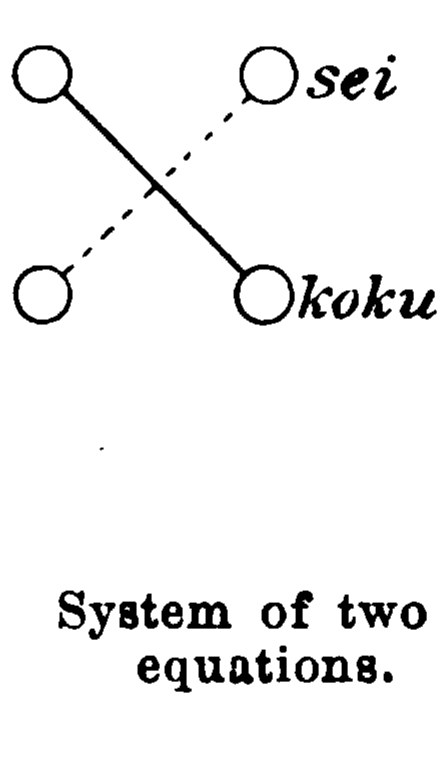
\includegraphics[width=\linewidth]{pdf211-shajo-two-equations.png}
\end{minipage}\hfill
\begin{minipage}[t]{.62\linewidth}
\centering
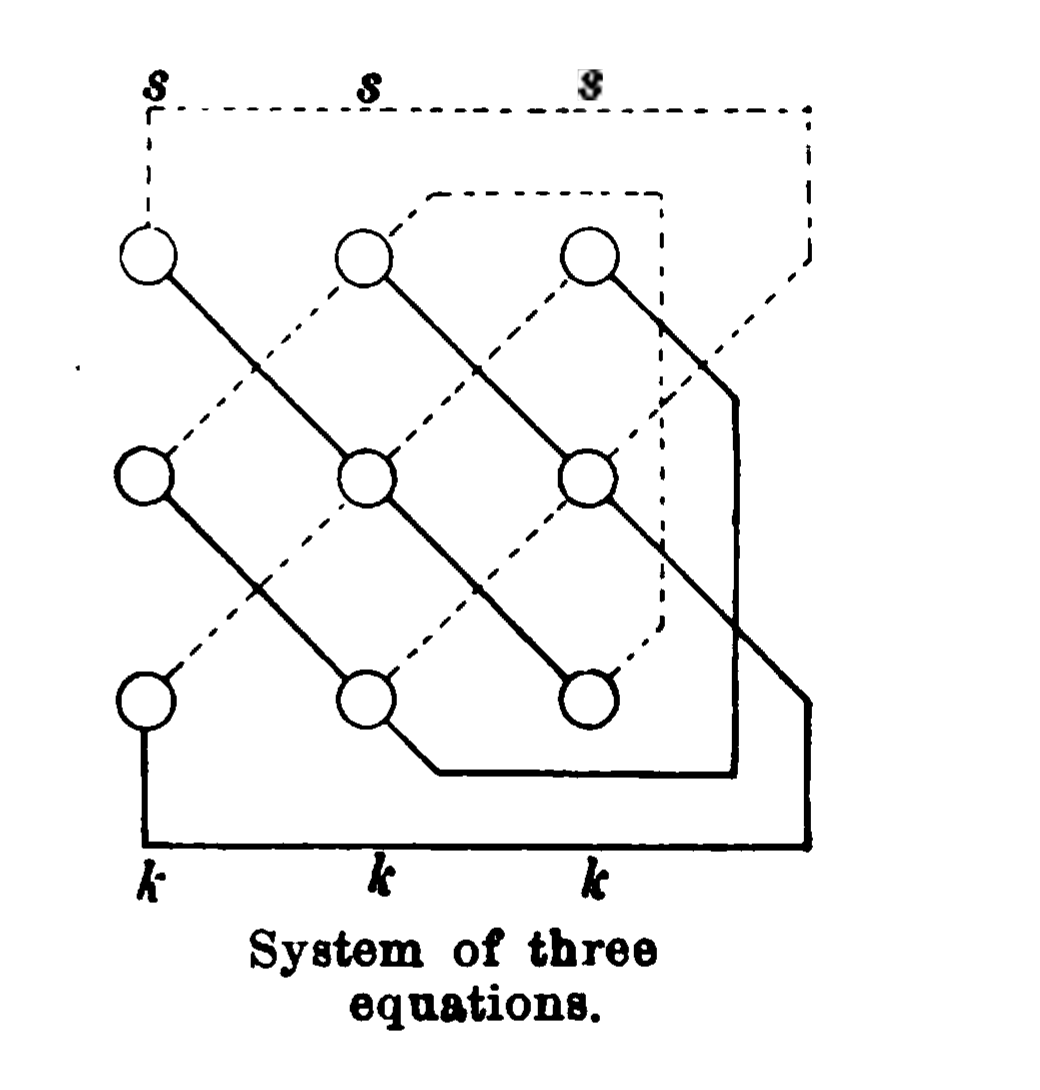
\includegraphics[width=\linewidth]{pdf211-shajo-three-equations.png}
\end{minipage}
\end{center}

It is obvious that the treatments may be extended to cases where there are more than five equations.

This operation is called \emph{shajō} or ``cross multiplication''.

\sourceassetJobAJ[width=.91\linewidth]{pdf211-shajo-diagrams-bottom.png}

14. There are of course still further terms not indicated in the diagrams, which are, however, all to be taken in actuality. To effect
\scanfooter

\scanpage{0212}{Chapter 24, printed page 198}
this, Seki employs the interchanges of the order in which the equations are taken. This operation is called \emph{kōshiki}. His statement is indeed very brief, but at the same time enough to indicate the nature of the procedure. He says thus:

``\emph{The kōshiki or interchanges of equations.} From the case of the three replacing equations that of the four will be derived; from that of the four equations that of the five will be derived; and so on. For the two or three replacing equations no \emph{kōshiki} or interchanges are necessary. Regular and reverse orders (\emph{jun} and \emph{gyaku}) are both to be successively increased by .1, and then we get the next order. For an odd number of replacing equations all are regular; for an even number the regular and reverse come alternately.''

This statement is accompanied by the following tables:\footnote{These tables should be read from right to left. The letters $o$ and $r$ stands for order and reverse.}

\sourceassetJobAJ[width=.92\linewidth]{pdf212-koshiki-tables.png}

The formation of successive sets is effected by taking one of the orders, for example, 2, 4, 3, 1, adding 1 to each of them, arranging 1 to the right of the set, whereby we get 3, 5, 4, 2, 1, and then constituting the middle set for the five equations.

The regular and reverse orders of interchanges will be seen from the diagrams. The former is effected to right-side and the latter to the left side in the above diagram.
\scanfooter

\scanpage{0213}{Chapter 24 conclusion, printed page 199}
When we carry out this operation together with that of the \emph{shajō} we are able to obtain·all the requisite terms in the expansion of a determinant. In Seki's book the \emph{kōshiki} is described before the \emph{shajō}.

15. When the \emph{sei} and \emph{koku} of the various terms have been determined, their respective signs are to be considered. If the given system be, for example,
\[
\begin{vmatrix}
I&F&C\\
H&E&B\\
G&D&A
\end{vmatrix}
\qquad\text{or}\qquad
\begin{vmatrix}
-1&4&-3\\
4&-5&1\\
-3&1&2
\end{vmatrix},
\]
we shall have
\[
\begin{array}{lll}
\emph{sei}&CEG=-45&\text{to be subtracted,}\\
\emph{sei}&IBD=-1&\text{”}\\
\emph{sei}&FHA=+32&\text{to be added,}\\
\emph{koku}&CHD=-12&\text{”}\\
\emph{koku}&FBG=-12&\text{”}\\
\emph{koku}&IEA=+10&\text{to be subtracted.}
\end{array}
\]

Of these several quantities those that are marked \emph{sei} are to be added when positive and subtracted when negative, while those marked \emph{koku} are to be subtracted when positive and added when negative.

In this way the desired elimination is effected, leading to an equation that does not contain the quantity eliminated, and that serves the purpose of solving the problem from which we have started.

From what we have said, it is very clear that Seki was possessed of the notion of determinants. And indeed he even indicates, if obscurely, the applicability of his theory to the cases of the determinants of orders higher than those considered by him. The theory does not however seem to have developed since the days of its expounder during the whole period in which flourished the mathematicians of the old Japanese school. It is rather curious that the determinant that had been so ingeniously practised in the elimination of a quantity between two equations that contain it did not happen to be applied to the solution of other kinds of problems, such as for example the linear simultaneous equations, etc.
\scanfooter

\scanpage{0214}{Chapter 25 opening, printed page 200}
\begin{center}
CHAPTER 25.\\[1mm]
THE VALUES OF $\pi$ USED BY THE JAPANESE MATHEMATICIANS.
\end{center}
\phantomsection\addcontentsline{toc}{subsection}{Chapter 25. The Values of $\pi$ Used by the Japanese Mathematicians}

The value of $\pi$ used by the Japanese in old times from somewhere about the 10th century and downwards through the whole reign of the Ashikaga Shogunate (14--16 centuries) was $3\cdot16$.\footnote{T. Endō, \emph{A short account on the progress about the values of $\pi$ in Japan} (in Japanese), in the \emph{Rigakkai}, vol. 3, no. 3, p. 19.} This same value of $\pi$ is referred to in the \emph{Kwatsuyō Sampō}\footnote{A posthumous publication of Seki's writings.} of 1709 as the old Japanese value.

Yoshida's \emph{Jinkōki} of 1627 was a treatise mainly based on the Chinese Ch'êng Tai-wei's work of 1593, but he did not adopt the value of $\pi$ given there. On the contrary he used the value $\pi=3\cdot16$. Imamura gave in his \emph{Jugai-roku} of 1639 the value $\pi=3\cdot162$, which his pupil Andō Yūyeki took to be obtained from $\pi^2=10$ in a commentary on the same work, published in 1660. Imamura's value of $\pi$ was followed by Yamada (1658), Shibamura (1657), Isomura (1660), etc.

Previous to 1660 the Japanese did not try the quadrature of the circle by applying the inscribed polygons with more than 32 sides, so that their values remained naturally very incorrect.\footnote{Endō in the article referred to, p. 20.} But there soon appeared an attempt leading to a more exact result. Muramatsu Mosei wrote the \emph{Sansō} in 1663, in which he published his measurement of the circle. He got from the perimeter of an inscribed $2^{15}=32768$-gon
\[
\pi=3\cdot14159\ 26487\ 77698\ 86924\ 8.
\]
This is correct to eight figures but the author did not know how far it was correct, and so he was obliged to compare it to Tsu Ch'ung-chih's value $\pi=22/7=3\cdot142657\ldots$ and to take $\pi=3\cdot14$. Nozawa Teichō gave the same value in his \emph{Dōkai-shō} of 1664. Satō Seikō gave $\pi=3\cdot142$ in his \emph{Kongenki} of 1666. Sumida Kōwun employed this value.\footnote{Endō's article, p. 19.} Imamura used in the decline of his life the values $\pi=3\cdot14$ and $\pi=3\cdot1416$.\footnote{Ibid.} Isomura revised in the second edition of his work (1684) the value of $\pi$, giving $3\cdot1416$. In 1696 Ikeda Shōi gave the value $\pi=3\cdot141662$ or $\pi=3\cdot142$ in his \emph{Gyokuyen Kyoku-seki}. In the \emph{Sampō Zusetsu} of 1704 Itō Yūkō gave $\pi=3\cdot1416$. This work appears to have been
\scanfooter

\scanpage{0215}{Chapter 25, printed page 201}
printed some years later. The value $\pi=3\cdot162=\sqrt{10}$ was used by so late a writer as Kambara Ichigaku in his \emph{Sankan-ki} of 1718. The value of $\pi$ equivalent to $\sqrt{10}$ is still being used in some parts of Japan by carpenters and timbermen.

Tsu Ch'ung-chih's two fractional values, $\pi=\frac{22}{7}$ and $\pi=\frac{355}{113}$, were reobtained in Japan by Seki Kōwa. Of these the former was learned from Chinese treatises but the latter seems to have been calculated by him anew. It was first published by his pupil Takebe Kenkō in the \emph{Kenki Sampō} of 1683. That this value had been given by Seki is stated by Takebe himself in his \emph{Fukyū Tetsujutsu} of 1722. The same value was also given in Ōtaka's \emph{Kwatsuyō Sampō} of 1709.

As it is not possible for us to account for every value of $\pi$ used in Japan, we feel we are obliged to restrict ourselves to giving only the most important results.

In the \emph{Kwatsuyō Sampō}, Book 4, of 1709, the circle-measurement is tried by numerical calculations using the inscribed polygons from the square up to a $2^{17}$-gon. The perimeters of the $2^{15}$-, $2^{16}$- and $2^{17}$-gons are found to be
\[
\begin{aligned}
\text{(a)}\quad 2^{15}\text{-gon}&=3\cdot14159\ 26487\ 76985\ 6708,\\
\text{(b)}\quad 2^{16}\text{-gon}&=3\cdot14159\ 26523\ 86591\ 3571,\\
\text{(c)}\quad 2^{17}\text{-gon}&=3\cdot14159\ 26532\ 88992\ 7759,
\end{aligned}
\]
from which a rectification is tried as follows:
\[
\pi=\frac{(b-a)(c-b)}{(b-a)-(c-b)}+b=3\cdot14159\ 26535\ 9.
\]

From this value of $\pi$ the following fractions are derived:
\[
\frac31,\frac72,\frac{10}3,\frac{13}4,\frac{16}5,\frac{19}6,\frac{22}7,\frac{25}8,
\frac{29}9,\frac{32}{10},\frac{35}{11},\frac{38}{12},\frac{41}{13},\frac{44}{14},\frac{47}{15},\frac{51}{16},
\]
\[
\frac{54}{17},\frac{57}{18},\ldots,\frac{355}{113}.
\]

In the anonymous manuscript \emph{Taisei Sankyō}\footnote{This is sometimes referred to Seki and sometimes to his pupil Takebe.} a repeated application of the rectification process as given above is attempted. Thus from the perimeters of the inscribed polygons from the square up to the 512-gon the following value is arrived at:
\[
\pi=3\cdot14159\ 26535\ 89793\ 23846\ 2643,
\]
\scanfooter

\scanpage{0216}{Chapter 25, printed page 202}
where the first 25 figures are correctly given. Again proceeding from this numerical value, the formula
\[
\frac{\pi}{1}=3+\frac{R_1}{1}=3+\frac{1}{\dfrac{1}{R_1}}=3+\frac{1}{Q_1+\dfrac{R_2}{R_1}}=\cdots
\]
will enable us to find the fractional values of $\pi$ thus:
\[
\frac31,\frac{22}7,\frac{333}{106},\frac{355}{113},\frac{103993}{33102},\frac{104348}{33215},\frac{208341}{66317},\frac{312689}{99532},\frac{837719}{265381},
\]
\[
\frac{11\ 46408}{3\ 64913},\qquad \frac{42\ 72943}{13\ 60120},\qquad\text{etc.}
\]

Takebe Kenkō employs in his \emph{Fukyū Tetsujutsu} of 1722 the same way of quadrature as followed in the \emph{Taisei Sankyō}, and from the inscribed 1024-gon he gets the value:
\[
\pi=3\cdot14159\ 26535\ 89793\ 23846\ 26433\ 83279\ 50288\ 41971\ 2,
\]
of which the first 41 figures are correct, the last figure being not included. Matsunaga Ryōhitsu gave in his manuscript \emph{Hōyen Sankyō} of 1739 the value:
\[
\pi=3\cdot14159\ 26535\ 89793\ 23846\ 26433\ 83279\\
\phantom{\pi={}}50288\ 41971\ 69399\ 3751,
\]
where 50 figures are given all correct. It was calculated from the series:
\[
\frac{\pi}{3}=1+\frac{1^2}{4\cdot6}+\frac{1^2\cdot3^2}{4\cdot6\cdot8\cdot10}+\frac{1^2\cdot3^2\cdot5^2}{4\cdot6\cdot8\cdot10\cdot12\cdot14}+\cdots.
\]

The same value of $\pi$ was published by Arima in his \emph{Shūki Sampō} of 1769, where the two fractions are also found:
\[
\pi=\frac{54\ 19351}{17\ 25033},\qquad \pi=\frac{42822\ 45933\ 49304}{13630\ 81215\ 70117},
\]
which give the first 13 and 30 figures of $\pi$ correctly.

Kurushima Yoshita (deceased in 1757) gave in his \emph{Kyūshi Ikō} or \emph{Kurushima's Posthumous Writings} the fractional values of $\pi^2$ as follows:
\[
\frac{227}{23},\qquad \frac{10748}{1089},\qquad \frac{10975}{1112},\qquad\text{and}\qquad \frac{98548}{9885}.
\]

About contemporary with Takebe and Matsunaga there was another mathematician Takuma Genzayemon who tried the quadrature of the circle by numerical calculations employing inscribed as well as circumscribed polygons of $2^{42}$ sides, whose perimeters are found to be
\scanfooter

\scanpage{0217}{Chapter 25 conclusion and Chapter 26 opening, printed page 203}
\[
3\cdot14159\ 26535\ 89793\ 23816\ 26433\ 6658,
\]
\[
3\cdot14159\ 26535\ 89793\ 23846\ 26433\ 67,
\]
and taking the average of these two, the value of $\pi$ correct to 26 figures was established as follows\footnote{Endō's article, No. 4, pp. 21--22.}:
\[
\pi=3\cdot14159\ 26535\ 89793\ 23846\ 26433.
\]

\begin{center}
CHAPTER 26.\quad JAPANESE MATHEMATICIANS' STUDIES\\[1mm]
OF THE SPHERICAL VOLUME.
\end{center}
\phantomsection\addcontentsline{toc}{subsection}{Chapter 26. Japanese Mathematicians' Studies of the Spherical Volume}

1. The Japanese mathematicians of the 17th century gave various values to the volume of a sphere, the earliest instances of which were Imamura's \emph{Jugairoku} of 1639 and a new edition of Yoshida's \emph{Jinkōki}. Imamura's value of the spherical volume of unit diameter was $0\cdot51$. Yoshida gave the value $0\cdot5625$.\footnote{This value was not given in the \emph{Jinkōki} of 1627. It was contained in a later edition in which some questions were proposed for solution. This edition has been lost.} This is too large as will be seen easily. Yamada published the \emph{Kaisanki} in 1656 and corrected it, taking to be less than $0\cdot5$. The values given by subsequent writers are:

\begin{center}
\begin{tabular}{l|l|c|c}
\text{author}&\text{title}&\text{date}&\text{value}\\ \hline
Shibamura&Kakuchi Sansho&1657&$0\cdot525$\\
Isomura&Ketsugi-shō&1660&$0\cdot510$\\
Muramatsu&Sansō&1663&$0\cdot524$\\
Nozawa&Dōkaishō&1664&$0\cdot523$\\
Satō&Kongen-ki&1666&$0\cdot519$\\
Okuda&Shimpen Sansūki&1681&$0\cdot555$\\
Isomura&(2nd edition)&1684&$0\cdot5236$\\
Miyagi&Wakan Sampō&1695&$0\cdot51$
\end{tabular}
\end{center}

In the times of these writers the way of calculating the spherical volume consisted in dividing the sphere into slices of equal thickness by parallel planes, taking for the volume of one of these slices the average of those of the cylinders upon its two bases and with the same altitude, and summing up the results for all the slices. The differences in the final values resulted from the different numbers into which the sphere is divided and the different values for the area-coefficient of the circle employed.
\scanfooter

\scanpage{0218}{Chapter 26, printed page 204}
For example's sake what Isomura says in the 1684 edition of his \emph{Ketsugishō} will be reproduced below:

``If we cut a sphere of diameter 1 foot into 10000 slices, the thickness of each slice is $0\cdot0001$ feet, which will be something like that of a very thin paper. Finding in this way the volume of each of them, we sum up the results, 10000 in number, when we get $523\cdot6$ measures.\footnote{Here the unit is the cube of the tenth part of a foot.} Besides, it is true, there are small incommensurable parts, which are neglected.''

2. In Ōtaka's \emph{Kwatsuyō Sampō}, which was Seki Kōwa's posthumous work, there is a chapter devoted to the evaluation of the spherical volume. Following a similar consideration as done by his predecessors Seki cuts the sphere into 50, 100 and 200 pieces and finds their sums to be
\[
a=0\cdot6664,\qquad b=0\cdot6666,\qquad c=0\cdot66665,
\]
where the factor $\frac14\pi$ is neglected. A rectification process as employed in the calculation of the circumference of a circle (see p. 201) will give from these three quantities the value $0\cdot666\frac23$. This being multiplied by $\frac{\pi}{4}=\frac14\times\frac{355}{113}$, the final result for the spherical volume is obtained to be
\[
0\cdot523\frac{203}{339}=\frac{355}{6\times113}=d^3\times\frac{\pi}{6}.
\]

3. Matsunaga considered in his \emph{Sampō Shūsei} this way of calculating the volume of a sphere as unsatisfactory and tried to give a better treatment, which is analytical.

Suppose a sphere is divided into $n$ slices of equal thickness. The sagittae of the spherical caps with the sections to their bases will be denoted by $s_1$, $s_2$, $s_3$, \ldots, being counted in order of magnitude. Then $d$ being the diameter of the sphere, these lengths are evidently equal to
\[
\frac dn,\quad \frac{2d}{n},\quad \frac{3d}{n},\quad\ldots.
\]
The diameters of the circles of the sections, denoted by $c_1$, $c_2$, \ldots, may be expressed by the formula:
\[
c_r^2=4(d-s_r)s_r=4rds_1-4r^2s_1^2.
\]
Multiplying by $\frac14\pi$ and by the common thickness, which is equal to $s_1$, and summing up, we have
\[
4\times\frac{\pi}{4}\times ds_1^2(1+2+3+\cdots+n)-4\times\frac{\pi}{4}\times s_1^3(1^2+2^2+3^2+\cdots+n^2)
\]
\[
=\pi ds_1^2\left(\frac{n^2}{2}+\frac n2\right)-\pi s_1^3\left(\frac{2n^3}{6}+\frac{3n^2}{6}+\frac n6\right)=\frac{\pi}{6}\times d^3-\frac{\pi}{6}\times d^3\times\frac1{n^2}.
\]
\scanfooter

\scanpage{0219}{Chapter 26, printed page 205}
Here the number of divisions, $n$, may be conceived as large as we please, so that the reciprocal of its power may be made as small as we please. Consequently this latter may be neglected in the end, when we get $\frac16\pi d^3$ for the volume of the sphere.

This same proceeding is also followed in the same author's \emph{Ritsuyen Ritsu} (Analysis for the Sphere), his pupil Yamaji's \emph{Gyokuseki Shinjutsu} (Exact Method of finding the Spherical Volume), the anonymous \emph{Kigenkai} that bears a second title \emph{Yenri Kenkon Sho} and that is sometimes referred to as containing Seki's methods. Some scholars are on that account of the opinion that the analysis we have just described was due to him.\footnote{T. Endō, in the Proc. of Tokyo M. P. S., vol. 7, pp. 123--126.}

4. The same way of analysis may be equally applied to the case of a spherical segment, which is recorded in the manuscripts mentioned above. If the segment is divided into $n$ parts by sections parallel to its base, whereby the sagitta $s$ is cut into $n$ parts all equal to $\frac1n s$, and if the diameters of the section circles be denoted by $c_1$, $c_2$, \ldots, which are counted beginning at the end of the sagitta, we shall have
\[
c_r^2=4\left(d-r\times\frac{s}{n}\right)r\frac{s}{n}=\frac{4ds}{n}\times r-\frac{4s^2}{n^2}\times r^2,
\]
\[
\therefore\sum_{r=1}^{r=n}c_r^2=\frac{4ds}{n}\sum_{r=1}^{r=n}r-\frac{4s^2}{n^2}\sum_{r=1}^{r=n}r^2
=\frac{4ds}{n}\times\frac{n+n^2}{2}-\frac{4s^2}{n^2}\times\frac{n+3n^2+2n^3}{6},
\]
\[
\therefore\frac{\pi}{4}\times\frac{s}{n}\times\sum_{r=1}^{r=n}c_r^2
=\frac{\pi}{6}\times s^2\times\left\{\frac{3d}{n}+3d-\frac{s}{n^2}-\frac{3s}{n}-2s\right\},
\]
whence, going to the limit $n=\infty$, we obtain the volume of the segment to be $=\frac16\pi s^2(3d-2s)$.

The above way of finding the volumes of a sphere and a spherical segment may have served the progress of the infinitesimal considerations in the \emph{yenri} method of the Japanese mathematics. Ajima's improvement of the circular theory by introducing the equal divisions of the diameter or a chord of a circle instead of equally dividing an arc or the circumference, as had been done by his predecessors, was certainly effected in imitation of the treatment of the sphere.

5. Wada Nei (1787--1840) took the element of volume
\[
\left\{d^2-\left(r\times\frac dn\right)^2\right\}\cdot\frac dn\cdot\frac\pi4=d^3\frac\pi4\left(\frac1n-\frac{r^2}{n^3}\right),
\]
\scanfooter

\scanpage{0220}{Chapter 26 conclusion and Chapter 27 opening, printed page 206}
and effected upon it the operation of ``folding'' or of integration by means of a table, thus getting at once the expression
\[
d^3\times\frac\pi4\left(1-\frac13\right)=\frac16d^3\pi.
\]

Wada's predecessors had always gone through all the steps of summing up the elements and finding the limiting value of the sum, but the use of a ``folding table'' enabled him to strike all this in a single operation. And thus a considerable amount of labour was saved.

\begin{center}
CHAPTER 27.\\[1mm]
JAPANESE MATHEMATICIANS' STUDIES OF FINDING THE\\
SURFACE OF A SPHERE.
\end{center}
\phantomsection\addcontentsline{toc}{subsection}{Chapter 27. Japanese Mathematicians' Studies of Finding the Surface of a Sphere}

1. Imamura Chishō gave in his \emph{Jugai-roku} of 1639 the surface of a sphere by the fourth part of the square of its circumference. The same was adopted by Isomura in his \emph{Ketsugi-sho} of 1660. It appears, this was in common use among the Japanese mathematicians of those times, for Isomura refers to it in the second edition of his work, published in 1684, as the old method. The incorrectness of the formula was noticed by him in this edition, but according to him, those mathematicians, Mōri, Yoshida, Imamura, Takahara, Hiraga, Shimada, Sumida and others had not been able to find a correct one for the spherical surface. Isomura tried the measurement thus:

The volumes of the spheres, whose diameters are 10 and $10\cdot0002$, being $523\cdot6$ and $523\cdot63141\ 66283\ 24188\ 8$, respectively, their difference is $0\cdot03141\ 66283\ 24188\ 8$. Dividing it by the thickness $0\cdot0001$ of the rind comprised between the two surfaces, we get $314\cdot16628\ 32418\ 88$ as the surface of the rind with the thickness of $0\cdot0001$. Again the volume of the sphere of diameter $9\cdot9998$ is $523\cdot56858\ 64283\ 15811\ 2$, and its difference from that of the sphere of diameter 10 being divided by the thickness $0\cdot0001$, the surface of the rind in this case will be found to be $314\cdot15371\ 68418\ 88$. The surface of the sphere will be given by the average of these two areas, or by
\[
314\cdot16000\ 00418\ 88.
\]
But the volume of the sphere being $523\cdot6$, we have
\[
523\cdot6\times6=3141\cdot6,
\]
so that it follows that
\[
(\text{surface})=\frac{(\text{volume})\times6}{(\text{diameter})},\qquad\text{or}= (\text{diameter})^2\times\pi.
\]
\scanfooter

\scanpage{0221}{Chapter 27, printed page 207}
2. The same way of evaluating the surface of a sphere as done by Isomura was adopted also by Takebe Kenkō in his \emph{Fukyū Tetsujutsu}, of 1722. Takebe did not however take the average of two values but proceeded otherwise. Forming the rinds of the spheres of diameters $10\cdot01$, $10\cdot0001$ and $10\cdot00000\ 01$, by taking away the sphere of diameter 10 from them, Takebe finds their quotients by the respective thicknesses to be
\[
314\cdot47352\ 9344,\qquad 314\cdot16240\ 6984,\qquad 314\cdot15929\ 677,
\]
and applies to these the rectification process as given in Ōtaka's \emph{Kwatsuyō Sampō}. Thus, denoting these values by $a$, $b$ and $c$, the rectified value of the spherical surface is obtained to be
\[
(\text{surface})=b-\frac{(a-b)(b-c)}{(a-b)-(b-c)}=314\cdot15926\ 5359.
\]

Seeing that this value is the same as that of $\pi$, except for the positions of the figures, Takebe at once writes $(\text{diameter})^2\pi$ for the surface of the sphere.

3. According to Takebe's \emph{Fukyū Tetsujutsu}, Seki applied a different way of consideration for the same purpose. Seki considered the centre of the sphere as the vertex of a cone, taking the radius as the altitude and the spherical volume as that of the cone. Thus we have
\[
\frac13(\text{surface})(\text{radius})=(\text{volume of cone})=(\text{volume of sphere}),
\]
\[
\therefore\quad (\text{spherical surface})=\frac{3\times(\text{spherical volume})}{(\text{radius})},
\]
a result that agrees with the formula given by Isomura.

Seki, who had used such a method of attack as here mentioned, despised the procedure established by Isomura and Takebe as little worthy. But Takebe emphasizes that he does not agree with Seki.

4. The anonymous manuscript \emph{Kigen-kai}, of which mention has already been made, contains a chapter on the evaluation of the surface of an ellipsoid of revolution, whose axis of revolution is $a=1$ foot, the other axis being $b=0\cdot6$ feet. Subtracting the volume of this ellipsoid from those for which the values of $a$ and $b$ are
\[
\begin{array}{c|c|c|c|c}
a&1\cdot001&1\cdot0001&1\cdot00001&1\cdot000001\\
b&0\cdot601&0\cdot6001&0\cdot60001&6\cdot000001
\end{array},
\]
and dividing the differences by the respective thicknesses of the rinds or by $0\cdot0005$, $0\cdot00005$, $0\cdot000005$, $0\cdot00000\ 05$, the results will be found, except for the factor $\frac16\pi$ which is neglected, to be
\scanfooter

\scanpage{0222}{Chapter 27, printed page 208}
\[
\begin{aligned}
A&=3\cdot12440\ 2,&\qquad C&=3\cdot12004\ 40002,\\
B&=3\cdot12044\ 002,&D&=3\cdot12000\ 44000\ 02.
\end{aligned}
\]
The successive differences of these values are
\[
F=0\cdot00396\ 198,\qquad H=0\cdot00039\ 60198,
\]
\[
K=0\cdot00003\ 96001\ 98;
\]
\[
\therefore\quad \frac HF=\frac{6667}{66700},\qquad \frac KH=\frac{66667}{6\ 66700},\qquad\text{or}\qquad \frac{H\mid F}{K\mid H}=\frac{444\ 48889}{444\ 66889}.
\]
Here it is argued, that as this last quantity does not become unity no conclusion could be drawn therefrom. Consequently the author strikes a different way.

The difference of the volumes of the two ellipsoids $(a,b)$ and $(a'=a+2h,b'=b+2h)$ being divided by $h$, the quotient is, the factor $\frac16\pi$ being put aside,
\[
\frac{(a+2h)(b+2h)^2-ab^2}{h}=4ab+2b^2+h(4a+8b+8h).
\]

Taking the values of $a$ and $b$ as given above, and putting
\[
2h=0\cdot001,\quad 0\cdot0001,\quad 0\cdot00001,\quad 0\cdot00000\ 1,
\]
the quantity multiplied by $h$ in the above expression assumes the values:
\[
\begin{aligned}
A'&=0\cdot00440\ 2,&\qquad C'&=0\cdot00004\ 40002,\\
B'&=0\cdot00044\ 002,&D'&=0\cdot00000\ 44000\ 02.
\end{aligned}
\]

If we take away these quantities from what we have designated $A$, $B$, $C$, $D$, respectively, the remainders will be found equal. If we then consider that in the actual case there is nothing as thickness, we may neglect the terms multiplied by $h$. Thus, restoring the neglected factor $\frac16\pi$, the surface will be given by
\[
\frac\pi6(4ab+2b^2)=(b^2+2ab)\frac\pi3.
\]

This result is not correct but the idea of the procedure that has been followed may be of some interest in history.

5. In Tani Shōmo's manuscript of 1825 or 1827 entitled \emph{Tetsujutsu Shin-i} we see the problem of finding the surface of an ellipsoid of revolution attacked in a different way. His result is
\[
(\text{surface})=ab\pi\left(1-\frac m6-\frac{m^2}{40}-\frac{m^3}{112}-\frac{m^4}{1152}-\cdots\right),
\]
where $m$ is written for $1-\frac{b^2}{a^2}$. Writing $t=\frac{ab\pi}{\sqrt m}$, this may be written
\scanfooter

\scanpage{0223}{Chapter 27, printed page 209}
\[
\frac{(\text{surface})}{t}=\sqrt m-\frac{\sqrt{m^3}}6-\frac{\sqrt{m^5}}{40}-\frac{\sqrt{m^7}}{112}-\frac{\sqrt{m^9}}{1152}-\cdots,
\]
a formula that will be seen to represent the area of a portion of a circle of unit diameter comprised between two equal and parallel chords with the distance $\sqrt m$. But this latter area is $=\frac14\pi-2\times(\text{area of the segment whose chord is }c=\sqrt{1-m^2}=a/b)$, and thus Tani expresses the surface of the ellipsoid of revolution by the formula
\[
(\text{surface})=\frac1{\sqrt m}\left\{\frac\pi6\times\pi\times ab-2\times ab\pi\,(\text{segmental area})\right\}.
\]

Tani mentions, this formula was obtained also by Ikeda Teiichi's pupil Kinoshita Teichi and suspended before a Shintō temple in Yedo in 1823. The result was published by Shiraishi Chōchū in his \emph{Shamei Sampu} of 1826.

Tani also obtained a formula for the area of a part of the same solid cut off by two planes normal to the axis of revolution.

Shiraishi's measurement of the ellipsoidal surface will be considered in chapter 38.

6. Now to return to the subject of our topic, the way of finding the surface of a sphere from the difference of the volumes of two spheres was again employed by Wada Nei who was a contemporary of Tani. If in the same pursuit as Isomura and Takebe, yet Wada's consideration was effected in analytical way. If we take two spheres whose diameters are $d$ and $d+h$, the difference of their volumes is
\[
(d+h)^3\frac\pi6-d^3\frac\pi6=\frac\pi6(3d^2h+3dh^2+h^3).
\]

If this rind be considered as developed in a flat figure, its thickness will be $\frac12h$, so that its surface will be $\frac13\pi(3d^2+3dh+h^2)$. But since $h$ may be conceived as small as we please, this reduces in the limit to $\frac13\pi\times3d^2=d^2\pi$, which represents the area of the spherical surface. It will be seen that Wada's analysis agrees with that given in the \emph{Kigen-kai} for the ellipsoid of revolution.

7. In Hasegawa Kan's \emph{Sampō Shinsho} published in 1830, the same way of measuring the spherical surface was made public. In this place the following expression is made use of:
\[
(\text{surface})\times h=d^3\frac\pi6-(d-2h)^3\frac\pi6.
\]
\scanfooter


\scanpage{0224}{Chapter 28 opening, printed page 210}
\begin{center}
CHAPTER 28.\\[1mm]
A FORMULA FOR THE SQUARE OF AN ARC OF A CIRCLE IN\\
THE \emph{KWATSUYŌ SAMPŌ} OF 1709.
\end{center}
\phantomsection\addcontentsline{toc}{subsection}{Chapter 28. A Formula for the Square of an Arc of a Circle in the Kwatsuyō Sampō of 1709}

In the \emph{Kwatsuyō Sampō}, Book 4, compiled by Ōtaka Yūshō in 1709 from among Seki Kōwa's writings and published in 1712, there is a formula for the square of an arc of a circle. It is this:
\[
\begin{aligned}
12\,76900(d-s)^5(\mathrm{arc})^2={}&51\,07600d^6s-238\,35413d^5s^2\\
&+434\,70240d^4s^3-379\,97429d^3s^4+150\,47062d^2s^5\\
&-15\,01025ds^6-2\,81290s^7,
\end{aligned}
\]
where $d$ is the diameter and $s$ the sagitta.

Something is spoken of in the book about the construction of it, which is however little intelligible. But when we examine the explanations given in various manuscripts, such as the anonymous \emph{Kigenkai}, Matsunaga's \emph{Sampō Shūsei}, Ōba Keimei's \emph{Kwatsuyō Kojutsu no Kai} or ``A note on the formula for an arc of a circle in the \emph{Kwatsuyō Sampō}'', dated 1774, etc., the precedure becomes manifest. Here we propose to give a brief description of the analysis.

First of all, the arcs of a circle whose diameter is 1 foot and whose sagittae are $s_1=0\dd1$, $s_2=0\dd2$, $s_3=0\dd3$, $s_4=0\dd4$, $s_5=0\dd45$, $s_0=0\dd5$, are found by numerical calculations, which are effected by inscribing a regular polygonal line of two sides and successively doubling the number of sides until a $2^{15}=32768$-gonal line is reached. The same rectification process as tried in the case of the whole circumference, which we have already mentioned, being applied, and the results being multiplied by $\pi=\frac{355}{113}$ and divided by $\pi=3\dd14159\,26535\,9$ in order to keep correspondence with the fractional value of $\pi$, these arcs will be found to be
\[
\begin{aligned}
x_1&=0\dd64350\,11087\,93284\,3868,\\
x_2&=0\dd92729\,5218,\\
x_3&=1\dd15927\,94807\,3,\\
x_4&=1\dd36943\,84060\,1,\\
x_5&=1\dd47062\,89056\,3.
\end{aligned}
\]
Then for $r=1,2,3,4,5$ the quantities $\alpha_r$ are formed thus:
\[
\alpha_r=s_r^2k+4(d-s_r)s_r-x_r^2,
\]
\scanfooter

\scanpage{0225}{Chapter 28, printed page 211}
where $k$ is written for
\[
k=\frac{355^2-4\times113^2}{113^2}=5\dd86960\,60772\,18.
\]

It is evident that $\alpha_r$ vanishes if we write therein $s_r=\frac12d$ or $s_r=s_0$. These quantities $\alpha$ are called the ``differences of the arc square''. The numerical values of these differences are
\[
\begin{aligned}
\alpha_1&=0\dd00460\,23178\,51,\\
\alpha_2&=0\dd01490\,76696\,87,\\
\alpha_3&=0\dd02433\,54023\,45,\\
\alpha_4&=0\dd02377\,51122\,95,\\
\alpha_5&=0\dd01584\,54867\,58.
\end{aligned}
\]
Again the ``differences of the third powers'' are formed thus:
\[
\beta_r=\frac{m_1s_r^2(d-2s_r)}{d-s_r}-\alpha_r,
\]
where
\[
m_1=\frac{\alpha_1(d-s_1)}{(d-2s_1)s_1^2}=0\dd51776\,07582\,2,
\]
and then the following quantities will be formed:
\[
\begin{aligned}
m_2&=\frac{\beta_2(d-s_2)^2}{(d-2s_2)s_2^2(s_2-s_1)}=0\dd16670\,74826\,5,\\[1mm]
\gamma_r&=\frac{m_2(s_r-s_1)s_r^2(d-2s_r)}{(d-s_r)^2}-\beta_r,\\[1mm]
m_3&=\frac{\gamma_3(d-s_3)^3}{(d-2s_3)s_3^2(s_3-s_1)(s_3-s_2)}=0\dd07492\,90858\,3,\\[1mm]
\delta_r&=\frac{m_3(s_r-s_2)(s_r-s_1)s_r^2(d-2s_r)}{(d-s_r)^3}-\gamma_r,\\[1mm]
m_4&=\frac{\delta_4(d-s_4)^4}{(d-2s_4)s_4^2(s_4-s_1)(s_4-s_2)(s_4-s_3)}=0\dd04002\,63239\,5,\\[1mm]
\varepsilon_4&=\frac{m_4(s_r-s_3)(s_r-s_2)(s_r-s_1)s_r^2(d-2s_r)}{(d-s_r)^4}-\delta_r,\\[1mm]
m_5&=\frac{\varepsilon_5(d-s_5)^5}{(d-2s_5)s_5^2(s_5-s_1)\cdots(s_5-s_4)}=0\dd02523\,31671\,5,\\[1mm]
\zeta_r&=\frac{m_5(s_r-s_4)\cdots(s_r-s_1)s_r^2(d-2s_r)}{(d-s_r)^4}-\varepsilon_r.
\end{aligned}
\]

Here it is easy to see that $\beta_1$; $\gamma_1$, $\gamma_2$; $\delta_1$, $\delta_2$, $\delta_3$; $\varepsilon_1$, $\varepsilon_2$, $\varepsilon_3$, $\varepsilon_4$; $\zeta_1$, $\zeta_2$, $\zeta_3$, $\zeta_4$, $\zeta_5$; are all $=0$. If we write $\alpha_r=A$ and denote the first terms in the expressions for $\beta_r$, $\gamma_r$, $\delta_r$, $\varepsilon_r$, $\zeta_r$ by $B$, $C$, $D$, $E$, $F$ respectively, it will be evident that
\[
\zeta_r=F-E+D-C+B-A.
\]
\scanfooter

\scanpage{0226}{Chapter 28 conclusion, printed page 212}
But as $\zeta_r=0$ for $r=1,2,3,4,5$, we have
\[
A-B+C-D+E-F=0,
\]
which holds good for the values of $s_r$ that are equal to $s_1$, $s_2$, $s_3$, $s_4$, $s_5$. It also holds good for $s_r=s_0=\frac12d$, for $\beta$, $\gamma$, $\delta$, $\varepsilon$ all vanish, as is evident, for the same value of $s_r$. Thus the above relation, in which we now replace $x_r$ by $x$ and $s_r$ by $s$, that exists for $s=s_0,s_1,s_2,\ldots,s_5$, may be practically considered to exist for any other value of the sagitta $s$. Consequently this may be employed in determining the length of any arc whose sagitta is given.

The formula in the \emph{Kwatsuyō Sampō} represented in the above is a result that will be obtained from the relation we have just described by transforming and simplifying it.

The actual values of $\alpha$, $\beta$, $\gamma$, etc., are calculated to show that they tend to gradually diminish. The values of $\alpha$ have been already given. Those of $\beta$, $\gamma$, \ldots\ are
\[
\begin{array}{r@{\;}c@{\;}l|r@{\;}c@{\;}l}
\beta_2&=&0\dd00625\,15305\,99&\gamma_4&=&0\dd00606\,73806\,08\\
\beta_3&=&0\dd02292\,29379\,23&\gamma_5&=&0\dd00688\,39200\,96\\
\beta_4&=&0\dd03838\,79480\,99&\delta_4&=&0\dd00059\,29825\,77\\
\beta_5&=&0\dd03217\,52297\,65&\delta_5&=&0\dd00109\,59431\,02\\
\gamma_3&=&0\dd00157\,28554\,46&\varepsilon_5&=&0\dd00006\,66273\,69
\end{array}
\]

The reasoning in deriving the formula is thus very clear, but it remains at the same time very doubtful what had caused Seki to hit upon such a way. As to this point we earnestly long for the results of further studies. Its relation to the \emph{shōsa} method is also to be made clear. In any case the construction of the formula must be highly interesting from the historical point of view. If it is not so general as a formula expressed in an infinite series, still its value in history can by no means be looked upon as inferior to that of the latter. It may not improbably have been the key to the rise of the analytical considerations. It is rather astonishing that all this should hitherto have escaped the notice of historical writers on the Japanese mathematics.
\scanfooter

\scanpage{0227}{Chapter 29 opening, printed page 213}
\begin{center}
CHAPTER 29.\\[1mm]
SOME SERIES FOR $\pi$ USED BY THE JAPANESE\\
MATHEMATICIANS.
\end{center}
\phantomsection\addcontentsline{toc}{subsection}{Chapter 29. Some Series for $\pi$ Used by the Japanese Mathematicians}

We have already mentioned the values of $\pi$ used by the Japanese mathematicians of the 17th and 18th centuries. We propose in this place to give some of the infinite series given for $\pi$ and its powers by the scholars of the 18th and 19th centuries.

The first instance we meet with is the two series for $\pi^2$ obtained in Tanzan Shōkei's manuscript of 1728 entitled \emph{Yenri Hakki}. The analysis described there is ascribed to Takebe Kenkō. These two series are
\[
\tag{1}\pi^2=8\left(1+\frac16+\frac{1\dd4}{6\dd15}+\frac{1\dd4\dd9}{6\dd15\dd28}+\cdots\right),
\]
\[
\tag{2}\pi^2=4\left(1+\frac26+\frac{2\dd8}{6\dd15}+\frac{2\dd8\dd18}{6\dd15\dd28}+\cdots\right),
\]
which have been obtained from Takebe's series (given on p. 164) by writing $s=\frac12d$ and $s=d$, respectively.

Matsunaga gave in his \emph{Hōyen Sankyō} of 1739 or 1738 the two series
\[
\tag{3}\pi^2=9\left(1+\frac{1^2}{3\dd4}+\frac{1^2\dd2^2}{3\dd4\dd5\dd6}+\frac{1^2\dd2^2\dd3^2}{3\dd4\dd5\dd6\dd7\dd8}+\cdots\right),
\]
\[
\tag{4}\pi=3\left(1+\frac{1^2}{4\dd6}+\frac{1^2\dd3^2}{4\dd6\dd8\dd10}+\frac{1^2\dd3^2\dd5^2}{4\dd6\dd8\dd10\dd12\dd14}+\cdots\right).
\]
It is from the series (4) that Matsunaga calculated his value of $\pi$ correct to 50 figures.

In Sakabe's \emph{Tenzan Shinanroku} written in 1810 and printed in the next few years there is found the series:
\[
\tag{5}\pi=4\left(1-\frac15-\frac{1\times4}{5\dd7\dd9}-\frac{1\dd3\times4\dd6}{5\dd7\dd9\dd11\dd13}-\frac{1\dd3\dd5\times4\dd6\dd8}{5\dd7\cdots17}-\cdots\right).
\]

In Hasegawa Kan's \emph{Sampō Shinsho} printed in 1830 this series is indicated as obtained by combining each two terms, except the first term, of the series
\[
\tag{6}\frac{\pi}{4}=1-\frac16-\frac1{6\times5}-\frac{1\dd2}{6\times5\dd7}-\frac{1\dd2\dd3}{6\times5\dd7\dd9}-\frac{1\dd2\dd3\dd4}{6\times5\dd7\dd9\dd11}-\cdots.
\]

Hasegawa Kō gave in his \emph{Kyūseki Tsūkō} of 1844, published in his pupil Uchida Kyūmei's name, the series:
\[
\tag{7}\frac{\pi}{4}=1-\frac1{2\dd3}-\frac1{8\dd5}-\frac3{48\dd7}-\frac{15}{384\dd9}-\frac{105}{3840\dd11}-\cdots,
\]
\scanfooter

\scanpage{0228}{Chapter 29, printed page 214}
or rewritten in the form
\[
\tag{8}\frac{\pi}{4}=1-\frac1{3!}-\frac{1^2\dd3}{5!}-\frac{1^2\dd3^2\dd5}{7!}-\frac{1^2\dd3^2\dd5^2\dd7}{9!}-\cdots.
\]

Kawai Kyūtoku gave in his manuscript \emph{Shin Koyen-Jutsu} the series
\[
\tag{9}\pi=2\left(1+\frac{1^2}{3!}+\frac{3^2}{5!}+\frac{3^2\dd5^2}{7!}+\frac{3^2\dd5^2\dd7^2}{9!}+\cdots\right),
\]
\[
\tag{10}\frac{\pi}{4}=\frac23+\frac2{2\times3\dd5}+\frac{2\dd3}{2\times3\dd5\dd7}+\frac{2\dd3\dd4}{2\times3\dd5\dd7\dd9}+\frac{2\dd3\dd4\dd5}{2\times3\dd5\dd7\dd9\dd11}+\cdots.
\]
Of these two series Kawai says the former is inconvenient as its convergence is very slow. The series (8) is also found in this manuscript. Kawai was a pupil to Sakabe.

Wada Nei (1787--1840) is said to have given the following series:\footnote{T. Endō's article in the \emph{Rigakkai}, vol. 3, no. 4, p. 24.}
\[
\tag{11}\frac{\pi}{3}=1+\frac1{3\dd2\dd4}+\frac3{5\dd8\dd4^2}+\frac{15}{7\dd48\dd4^3}+\frac{105}{9\dd384\dd4^4}+\cdots,\footnotemark
\]
\footnotetext{The same as (4) given in a different form.}
\[
\tag{12}\frac{\pi}{2}=1+\frac1{3\dd2}+\frac3{5\dd8}+\frac{15}{7\dd48}+\frac{105}{9\dd384}+\cdots,
\]
\[
\tag{13}\frac{\pi}{4}=\frac13+\frac1{5\dd2}+\frac3{7\dd8}+\frac{15}{9\dd48}+\frac{105}{11\dd384}+\cdots,
\]
\[
\tag{14}\frac{\pi}{8}=\frac13+\frac1{15\dd2}+\frac3{35\dd8}+\frac{15}{63\dd48}+\frac{105}{99\dd384}+\cdots,
\]
\[
\tag{15}\frac{\pi}{32}=\frac1{15}+\frac1{35\dd2}+\frac3{63\dd8}+\frac{15}{99\dd48}+\frac{105}{143\dd384}+\cdots,
\]
\[
\tag{16}\frac{\pi}{4}=1-\frac13+\frac3{15}-\frac{15}{105}+\frac{105}{945}-\frac{945}{10395}+\cdots,
\]
\[
\tag{17}\frac{\pi}{8}=\frac7{15}+\frac{11\dd1}{105}+\frac{15\dd3}{945}+\frac{19\dd15}{10395}+\frac{23\dd105}{135135}+\cdots,
\]
\[
\tag{18}\frac{\pi}{2\sqrt2}=1+\frac1{3\dd2\dd2}+\frac3{5\dd8\dd2^2}+\frac{15}{7\dd48\dd2^3}+\frac{105}{9\dd384\dd2^4}+\cdots,
\]
\[
\tag{19}\frac{\pi}{8}=\frac12-\frac1{15}-\frac1{63}-\frac1{143}-\frac1{255}-\cdots.
\]

In Koide Shūki's manuscript \emph{Yenri Sankyō} of 1842, which was based upon Wada's writings, we find the two series:
\[
\tag{20}\frac{\pi}{4}=1-\frac13+\frac15-\frac17+\frac19-\frac1{11}+\cdots,
\]
\[
\tag{21}\frac{\pi}{4}=1-\frac1{3\dd2}-\frac1{5\dd8}-\frac3{7\dd48}-\frac{15}{9\dd384}-\frac{105}{11\dd3840}-\cdots,
\]
of which the former is the same as (16).
\scanfooter

\scanpage{0229}{Chapter 29, printed page 215}
The anonymous manuscript \emph{Sampō Yenri Hyō}, giving some tables required in the \emph{yenri} calculations, probably due to Wada, contains the series:
\[
\tag{22}\frac{\pi}{2\sqrt3}=1-\frac1{3\dd3}+\frac1{5\dd3^2}-\frac1{7\dd3^3}+\frac1{9\dd3^4}-\cdots,
\]
\[
\tag{23}\pi=\frac12\left(1-\frac1{2^2}-\frac3{8^2}-\frac{3\dd15}{48^2}-\frac{15\dd105}{384^2}-\cdots\right),
\]
\[
\tag{24}\pi=2\sqrt3\left(\frac1{3\dd2\dd2}+\frac1{5\dd8\dd2^2}+\frac1{7\dd48\dd2^3}+\frac1{9\dd384\dd2^4}+\cdots\right),
\]
\[
\tag{25}\pi^2=4\left(1+\frac2{2\dd3}+\frac8{3\dd15}+\frac{48}{4\dd105}+\frac{384}{5\dd945}+\cdots\right),
\]
\[
\tag{26}\pi^2=8\left(1+\frac2{2\dd3\dd2}+\frac8{3\dd15\dd2^2}+\frac{48}{4\dd105\dd2^3}+\frac{384}{5\dd945\dd2^4}+\cdots\right)\text{\footnotemark},
\]
\footnotetext{The same as a transformed form of (1).}
\[
\tag{27}\pi^2=9\left(1+\frac2{2\dd3\dd4}+\frac8{3\dd15\dd4^2}+\frac{48}{4\dd105\dd4^3}+\frac{384}{5\dd945\dd4^4}+\cdots\right).
\]

In the \emph{Yenri Sembi-Hyō}, an anonymous table, probably due to Wada, we see the series:
\[
\tag{28}\frac{\pi}{4}=1-\frac1{2^2}-\frac3{8^2}-\frac{3\dd15}{48^2}-\frac{15\dd105}{384^2}-\frac{105\dd945}{3840^2}-\cdots.
\]

Uchida Gokan's (1805--1882) \emph{Kojutsu Henkan Jenshū}, a manuscript, gives among others the following series:
\[
\tag{29}\pi\mathpunct{,}=\frac{3\sqrt3}{2}\left(1+\frac3{3\dd4\dd2}+\frac{3\dd3^2}{5\dd4^2\dd8}+\frac{15\dd3^3}{7\dd4^3\dd48}+\frac{105\dd3^4}{9\dd4^4\dd384}+\cdots\right),
\]
\[
\tag{30}\pi=3\sqrt3\left(1-\frac33+\frac{3^2}{5}-\frac{3^3}{7}+\frac{3^4}{9}-\frac{3^5}{11}+\cdots\right),
\]
\[
\tag{31}\pi=2\sqrt2\left(1+\frac1{3\dd2\dd2}+\frac3{5\dd2^2\dd8}+\frac{15}{7\dd2^3\dd48}+\frac{105}{9\dd2^4\dd384}+\frac{945}{11\dd2^5\dd3840}+\cdots\right).
\]
Of these (30) is apparently divergent.

We conclude this chapter by describing Tani Shōmo's considerations for deriving some formulae for $\pi$. These are taken from his \emph{Tetsujutsu Shin-i} of 1825 or 1827. Let
\[
P=c+c^3+\frac{3c^5}{40}+\frac{5c^7}{112}+\frac{35c^9}{1152}+\frac{63c^{11}}{2816}+\cdots,
\]
\[
Q=1-\frac{c^2}{2}-\frac{c^4}{8}-\frac{c^6}{16}-\frac{5c^8}{128}-\frac{7c^{10}}{256}-\cdots
\]
be the arc of a circle with unit diameter and with the chord $c$, and the length of the chord drawn perpendicular to $c$ at its end. From the expressions of $P$ and $Q$ follows easily:
\scanfooter

\scanpage{0230}{Chapter 29 conclusion, printed page 216}
\[
Q_1=P-cQ=\frac{2c^3}{3}+\frac{c^5}{5}+\frac{3c^7}{28}+\frac{5c^9}{72}+\frac{35c^{11}}{704}+\cdots,
\]
\[
Q_2=P-cQ-\frac{2c^3Q^3}{3}=\frac{8c^5}{15}+\frac{4c^7}{21}+\frac{c^9}{9}+\frac{5c^{11}}{66}+\cdots,
\]
\[
Q_3=P-cQ-\frac{2c^3Q}{3}-\frac{8c^5Q}{15}=\frac{16c^7}{35}+\frac{8c^9}{45}+\frac{6c^{11}}{55}+\cdots,
\]
\[
Q_4=P-cQ-\frac{2c^3Q}{3}-\frac{8c^5Q}{15}-\frac{16c^7Q}{35}=\frac{32c^9}{79}+\frac{64c^{11}}{385}+\cdots,
\]
\[
\cdots\cdots\cdots\cdots\cdots\cdots\cdots\cdots\cdots
\]
If we write $c=1$, then $Q$ vanishes, while from the series for $P$, $Q_1$, $Q_2$, \ldots, follow, after dividing by $\frac12$, the series:
\[
\tag{32}\pi=2+\frac13+\frac3{20}+\frac5{56}+\frac{35}{576}+\frac{63}{1408}+\cdots,
\]
\[
\tag{33}\pi=\frac43+\frac25+\frac3{14}+\frac5{36}+\frac{35}{352}+\cdots,
\]
\[
\tag{34}\pi=\frac{16}{15}+\frac8{21}+\frac29+\frac5{32}+\cdots,
\]
\[
\tag{35}\pi=\frac{32}{35}+\frac{16}{45}+\frac{12}{55}+\cdots,
\]
\[
\tag{36}\pi=\frac{64}{79}+\frac{128}{385}+\cdots,
\]
\[
\cdots\cdots\cdots\cdots\cdots\cdots\cdots\cdots
\]
Again let $A$ be the area of the circular segment with the chord $c$, then we have
\[
A=c-\frac{c^3}{6}-\frac{c^5}{40}-\frac{c^7}{112}-\frac{5c^9}{1152}-\frac{7c^{11}}{2816}-\cdots,
\]
\[
A-cQ^3=\frac{4c^3}{3}-\frac{2c^5}{5}-\frac{c^7}{14}-\frac{c^9}{36}-\frac{10c^{11}}{704}-\cdots,
\]
\[
A-cQ^3-\frac{4c^3Q^3}{3}=\frac{8c^5}{5}-\frac{4c^7}{7}-\frac{c^9}{9}-\frac{c^{11}}{12}-\cdots,
\]
\[
A-cQ^3-\frac{4c^3Q^3}{3}-\frac{8c^5Q^3}{5}=\frac{64c^7}{35}-\frac{22c^9}{45}-\frac{8c^{11}}{55}-\cdots,
\]
\[
A-cQ^3-\frac{4c^3Q^3}{3}-\frac{8c^5Q^3}{5}-\frac{64c^7Q^3}{35}=\frac{128c^9}{63}-\frac{64c^{11}}{77}-\cdots,
\]
\[
\cdots\cdots\cdots\cdots\cdots\cdots\cdots\cdots
\]
and writing $c=1$ we get
\[
\tag{37}\frac{\pi}{4}=1-\frac16-\frac1{40}-\frac1{112}-\frac5{1152}-\frac7{2816}-\cdots,
\]
\[
\tag{38}\frac{\pi}{4}=\frac43-\frac15-\frac1{14}-\frac1{36}-\frac{10}{704}-\cdots,
\]
\scanfooter

\scanpage{0231}{Chapter 29 conclusion and Chapter 30 opening, printed page 217}
\[
\tag{39}\frac{\pi}{4}=\frac85-\frac47-\frac19-\frac1{22}-\cdots,
\]
\[
\tag{40}\frac{\pi}{4}=\frac{64}{35}-\frac{32}{45}-\frac8{54}-\cdots,
\]
\[
\tag{41}\frac{\pi}{4}=\frac{128}{63}-\frac{64}{77}-\cdots,
\]
\[
\cdots\cdots\cdots\cdots\cdots\cdots\cdots\cdots
\]

\begin{center}
CHAPTER 30.\\[1mm]
KURUSHIMA'S CIRCLE-MEASUREMENT.
\end{center}
\phantomsection\addcontentsline{toc}{subsection}{Chapter 30. Kurushima's Circle-Measurement}

There is a manuscript entitled the \emph{Kyū-shi Kohai-Sō}, which means ``Kurushima's\footnote{Kurushima Yoshita was a scholar noted for the peculiarity of his character. He died in 1757.} results of Circle-Measurements'', a work that is of high interest in the Japanese mathematics. We give some of his results in the following lines.

1. Kurushima gives for the square of an arc of a circle ($a$) the expressions:
\[
\begin{aligned}
a^2={}&\frac1{315}\{(8192d-512s)s'+36s^2-788ds\}\\
&+\frac{832}{7425K}\{(3\,91936d^2-125296ds-59832s^2)s'-97984d^2s\\
&\hspace{42mm}+6828ds^2+10541s^3\},
\end{aligned}
\]
\[
\begin{aligned}
a^2=\frac4{51975K}\{&(1591\,33696d^2+3\,28473s^2-644\,50261ds)16s'\\
&+41404\,87466d^2s+308\,74623ds^2-1\,33429d^3\},
\end{aligned}
\]
where $d=$ diameter, $s=$ the sagitta, $s'=$ the sagitta of the arc $\frac12a$, and
\[
K=91910d-10425s-86064s'.
\]

In the above $s'$ is to be found from the equation, $ds-4ds'-4s'^2=0$, from which we have
\[
s'=\frac12\{d-\sqrt{d(d-s)}\}.
\]
Or, if we write
\[
A_1=4d/s-2,
\qquad A_2=A_1^2-2,
\qquad A_3=A_2^2-2,\ldots,
\]
and denote by $D_0$, $D_1$, $D_2$, \ldots\ the original term and the successive differences, namely, the 1st term and those that follow it, we shall have
\[
s'=\frac{s}{4}+\frac{D_0}{A_1}+\frac{D_1}{A_2}+\frac{D_2}{A_3}+\cdots.
\]
\scanfooter

\scanpage{0232}{Chapter 30, printed page 218}
Again Kurushima gives as inaccurate formulae for the arc square the following three:
\[
a^2=\frac{(5d-s)12ds}{15d-8s},
\qquad
a^2=\frac{\{(630d-195)d-23s^2\}4s}{45(14d-9s)},
\]
\[
a^2=\frac{[\{(14175d-5355s)d-840s^2\}d^2-172s^3]4s^2}{(45d-32s)315d}.
\]

He further gives the formulae
\[
\begin{aligned}
a^2={}&\frac1{(95d-81s)\,2412\,15975d^6}\{9\,16620\,70500d^3s\\
&-4\,75999\,52400d^7s^2-97581\,46100d^6s^3-34183\,74960d^5s^4\\
&-14825\,21040d^4s^5-7081\,05216d^3s^6-3466\,36800d^2s^7\\
&-1605\,68800ds^8-584\,55040s^9\},
\end{aligned}
\]
\[
a^2=16A/1\,43325B+4ds+\frac43s^2,
\]
where
\[
\begin{aligned}
A={}&2474\,33165\,91021\,68713\,24740d^4s^3\\
&-5217\,12944\,78069\,36920\,86006d^3s^4\\
&+3703\,39108\,13137\,53441\,10149d^2s^5\\
&-1003\,31457\,52198\,44044\,97600ds^6\\
&+80\,81700\,29592\,75826\,60800s^7,
\end{aligned}
\]
\[
\begin{aligned}
B={}&38843\,51113\,19021\,77602d^5\\
&-1\,06872\,38977\,48560\,61125d^4s\\
&+1\,09084\,65303\,66266\,52000d^3s^2\\
&-50472\,81827\,18611\,49040d^2s^3\\
&+10216\,76096\,82596\,05760ds^4.
\end{aligned}
\]

2. The ratio of sagitta and arc of a circular segment has a maximum value, as will be seen easily. This was observed by Kurushima for the first time in Japan, so far as we know. He tried to obtain by successive approximations the maximum value of $m=s\pi/ad$, where $s$, $a$, $d$ are written for sagitta, arc and diameter.

In the first place putting $d=1$, the sagittae $0\dd5$ and $1$ will give the values of $m$ to be both unity. Kurushima designates the corresponding arcs by the fractions $\frac12$ and $\frac11$. We shall denote these arcs by $\left[\frac12\right]$ and $\left[\frac12\right]$. The arc that arises from these two by virtue of the relation existing between the sagittae,
\[
s_3=\frac12\left\{\sqrt{s_1s_2}+d-\sqrt{s_1s_2+d^2-d(s_1+s_2)}\right\},
\]
\scanfooter

\scanpage{0233}{Chapter 30, printed page 219}
will be denoted by $\left[\frac34\right]$, the fraction being obtained as the average of $\frac12$ and $\frac11$; and so with other arcs. Then writing the values of $s$ and $m$ for $[p/q]$ by $s_{p/q}$ and $m_{p/q}$, Kurushima gives the following values:
\[
\begin{aligned}
s_{5/8}&=0\dd69341\,71618\,25448\,85857\,9,\\
m_{5/8}&=1\dd10614\,67458\,92071\,81737\,26,\\
s_{3/4}&=0\dd85355\,33905\,93273\,76220\,04,\\
m_{3/4}&=1\dd13807\,11874\,57698\,34960\,04,\\
s_{7/8}&=0\dd96193\,97662\,55643\,37806\,35,\\
m_{7/8}&=1\dd09935\,97328\,63592\,43207\,2.
\end{aligned}
\]
Thus the limiting value of $m$ will be seen to lie in the neighbourhood of $[3/4]$. Proceeding in this way Kurushima finds the values of $s$ and $m$ in the limit to be
\[
[s]=0\dd84457\,88682\,029,
\qquad [m]=1\dd13821\,68528\,69,
\]
and consequently he finds the square of the arc and its length to be
\[
[a]^2=5\dd43413\,15043\,04,
\qquad [a]=2\dd23112\,23700\,83.
\]

Kurushima tries still another proceeding for the same problem. Thus writing $x=$ the arc for which the quotient of the arc by its sagitta has the minimum value, and $y=$ the corresponding sagitta, we have\footnote{Here we have understood $d$ and its powers for simplicity's sake. Kurushima gives the formula for the sagitta in another part of the manuscript in the form
\[
(\mathrm{sagitta})=\frac{(\mathrm{arc})^2}{4d}\left\{1-\frac{(\mathrm{arc})^2}{3\dd4d^2}+\frac{(\mathrm{arc})^4}{3\dd4\dd5\dd6d^4}-\cdots\right\}.
\]
If we write $d=2$ and $x=$ half the arc, this formula becomes
\[
\mathrm{ver\ sin}\,x=\frac{x^2}{2!}-\frac{x^4}{4!}+\frac{x^6}{6!}-\cdots.
\]}
\[
-16y+4x^2-\frac{x^4}{3}+\frac{x^6}{3\dd5\times6}-\frac{x^8}{3\dd5\dd7\times6\dd8}+\frac{x^{10}}{3\dd5\dd7\dd9\times6\dd8\dd10}-\cdots=0,
\]
and Kurushima takes the equation
\[
-16y+8x^2-\frac{4x^4}{3}+\frac{x^6}{3\dd5}-\frac{x^8}{3\dd5\dd7\times6}+\frac{x^{10}}{3\dd5\dd7\dd9\times6\dd8}-\cdots=0
\]
without any further description, only saying it is obtained according to the ``method of the limiting value''. Taking the difference of the two equations, we get, on the removal of the superfluous factor $x^2$,
\[
4-x^2+\frac{x^4}{3\times6}-\frac{x^6}{3\dd5\times6\dd8}+\frac{x^8}{3\dd5\dd7\times6\dd8\dd10}-\frac{x^{10}}{3\dd5\dd7\dd9\times6\dd8\dd10\dd12}+\cdots=0,
\]
\scanfooter

\scanpage{0234}{Chapter 30, printed page 220}
which Kurushima calls an ``unlimited equation'' for the limiting arc, meaning an equation with an unlimited number of terms or an equation whose number of degrees is infinite. This equation is the same as we should obtain by differentiation after writing $y\mid x=u$. If Kurushima had not learned of the result of the differential calculus directly or indirectly from an European source, he may have deviced something that resembled the calculus to arrive at his rule for the limiting value. Or at least he may have extended the result given by Seki.\footnote{Consult Smith and Mikami's History for Seki's theory.} Unfortunately, however, we are not in position to make any guess on the matter, because Kurushima does not indicate the derivation of his process.

Kurushima goes on to try the solution of the above equation of the infinite degree. It will be of interest to see how he has attempted to get approximations. For that purpose he neglects the higher terms and successively takes 2, 3, 4, \ldots\ first terms. Thus he gets the following equations:
\[
4-x^2=0,
\qquad 72-18x^2+x^4=0,
\qquad 2880-720x^2+40x^4-x^6=0,
\]
\[
201600-50400x^2+2800x^4-70x^6+x^8=0,
\]
\[
217\,72800-54\,43200x^2+3\,02400x^4-756x^6+108x^8-x^{10}=0,
\]
etc., from which he obtains the roots, $x^2=4$, $6$, $5\dd4$, $5\dd435$, $5\dd434$.

These values will be seen to alternately increase and decrease and to successively approach a certain limit. Proceeding in this way Kurushima says that the first figures may be determined step by step. These correctly obtained figures are called ``pure'', while the succeeding figures that are not correct are called ``impure''. The impure figures are not easy to be corrected, but proceeding further and further in the evolutions, the impurity of remoter figures will disappear more and more. Thus saying, he calls this process the ``method of drawing the pure out of the impure'', in comparison to the appearance of pure draught by stillstanding out of impure mixture.

But Kurushima does not renew the solutions of the successive equations from the outset. He now takes the quantities:
\[
\begin{aligned}
A&=5\dd4,\\
a_1&=1-\frac{A}{9\dd12}=0\dd95,
& a_2&=1-\frac{a_1}{7\dd10}A=0\dd92671\,42,\\
a_3&=1-\frac{a_2}{5\dd8}A=0\dd87489\,356,
& a_4&=1-\frac{a_3}{3\dd6}A=0\dd73753\,2,\\
a_5&=1-\frac{a_4}{1\dd4}A=0\dd00433\,18;
& b_1&=4-\frac5{9\dd12}A=3\dd75,
\end{aligned}
\]
\scanfooter

\scanpage{0235}{Chapter 30, printed page 221}
\[
\begin{aligned}
b_2&=3-\frac{b_1}{7\dd10}A=2\dd7108,
& b_3&=2-\frac{b_2}{5\dd8}A=1\dd6341,\\
b_4&=1-\frac{b_3}{3\dd6}A=0\dd5098,
& b&=\frac{b_4}{1\dd4}=0\dd1274;
\end{aligned}
\]
and forms $a_5\mid b=0\dd034$, which will be added to $x^2=5\dd4$ to get a nearer approximation $x^2=5\dd434$.

The next step is to take $A=5\dd434$ and construct the quantities
\[
\begin{aligned}
4-A\Bigg\{1-\frac{A}{3\dd6}\Bigg[1-\frac{A}{5\dd8}\Bigg(1-\frac{A}{7\dd10}\Bigg\{1-\frac{A}{9\dd12}\Bigg[1-\frac{A}{11\dd14}\left(1-\frac{A}{13\dd16}\right)\Bigg]\Bigg\}\Bigg)\Bigg]\Bigg\},
\end{aligned}
\]
\[
1-\frac{A}{3\dd6}\Bigg\{2-\frac{A}{5\dd8}\Bigg(3-\frac{A}{7\dd10}\Bigg[4-\frac{A}{9\dd12}\Bigg\{5-\frac{A}{11\dd14}\left(6-\frac{7A}{13\dd16}\right)\Bigg\}\Bigg]\Bigg)\Bigg\},
\]
which are equal to
\[
K=0\dd00006\,6693,
\qquad H=0\dd50729,
\]
and to form $K\mid H=0\dd00013$. This being added to the previous value of the root, we have $x^2=5\dd43413$. This is done by the same principle as followed above.

Proceeding in this way, Kurushima deduces the next digits to be
\[
0\dd00000\,15,
\qquad 0\dd00000\,00043\,04,
\]
so that the final approximation is taken
\[
x^2=5\dd43413\,15043\,04.
\]

3. Again Kurushima gives an analytical expression for the square of the arc, which he derives from the equation we have mentioned above. His description is of cource very meagre, hardly intelligible to any reader of his manuscript. But when we carefully examine the meanings conveyed by the obscure language with which he has expressed his results, we are able to find out the paths followed by him. If namely we write
\[
x^2\ \text{or}\ (\mathrm{arc})^2=D_0+D_1+D_2+D_3+\cdots,
\]
we shall then have from the said equation
\[
\begin{aligned}
&D_0+D_1+\qquad D_2+\qquad D_3+\qquad D_4+\cdots\\
={}&4\\
&+\frac1{3\dd6}\{D_0^2+2D_0D_1+(2D_0D_2+D_1^2)+(2D_0D_1+2D_1D_2)+\cdots\}\\
&-\frac1{3\dd6\dd5\dd8}\{D_0^3+3D_0^2D_1+(3D_0^2D_2+3D_0D_1^2)+\cdots\}\\
&+\frac1{3\dd6\dd5\dd8\dd7\dd10}\{D_0^4+4D_0^3D_1+\cdots\}\\
&-\frac1{3\dd6\dd5\dd8\dd7\dd10\dd9\dd12}\{D_0^5+\cdots\}+\cdots.
\end{aligned}
\]
\scanfooter

\scanpage{0236}{Chapter 30 continuation, printed page 222}
Here the quantities within the crooked brackets in the successive lines represent the powers of $x^2$, and thus it will be seen that multiplication of series is employed. This operation has since been extensively applied by the Japanese mathematicians in the calculations concerning the circular theory.

Now equating the terms in above equation according to vertical columns, we have
\[
D_0=4,
\qquad D_1=\frac1{3\dd6}D_0^2,
\qquad D_2=\frac1{3\dd6}\left\{2D_0D_1-\frac1{5\dd8}D_0^3\right\},
\]
\[
D_3=\frac1{3\dd6}\left\{(2D_0D_2+D_1^2)-\frac1{5\dd8}\left(3D_0^2D_1-\frac1{7\dd10}D_0^4\right)\right\},
\]
\[
D_4=\frac1{3\dd6}\left\{(2D_0D_3+2D_1D_2)-\frac1{5\dd8}\left[(3D_0^2D_2+3D_0D_1^2)-\frac1{7\dd10}\left(4D_0^3D_1-\frac1{9\dd12}D_0^5\right)\right]\right\},
\]
etc. The numerical values of the $D$'s are calculated to be
\[
\begin{array}{r@{\;}c@{\;}l@{\qquad}r@{\;}c@{\;}l}
D_0&=&4,&D_1&=&0\dd88888\,88\ldots,\\
D_2&=&0\dd30617\,28\ldots,&D_3&=&0\dd12579\,26\ldots,\\
D_4&=&0\dd05689\,376\ldots,&D_5&=&0\dd02734\,05\ldots,
\end{array}
\]
and the sum of $D_5$ and further terms resulting to be $=0\dd0526\ldots$, we have
\[
x^2=5\dd43037\,796\ldots.
\]

Dividing $D_1$ by $D_0$, $D_2$ by $D_1$, and so on, finally the formula for the square of the arc is obtained in the form
\[
4+\frac29D_0+\frac{31}{90}D_1+\frac{4012}{9765}D_2+\frac{16331}{36108}D_3+\frac{90\,64366}{188\,62305}D_4+\cdots.
\]
Thus Kurushima has effected the reversion of series by a numerical way.

Next to express the value of the limiting sagitta by an infinite expansion, the same process as given above will apply, first taking the series
\[
(\mathrm{sagitta})=\frac{(\mathrm{arc})^2}{4}-\frac{(\mathrm{arc})^4}{4\times3\dd4}+\frac{(\mathrm{arc})^6}{4\times3\dd4\dd5\dd6}-\cdots,
\]
and substituting the same expression for the powers of $(\mathrm{arc})^2$ as above and grouping in like way. Thus we have
\[
D_0'=\frac{D_0}{4}=1,
\qquad
D_1'=\frac14\left\{\frac1{3\dd4}D_0^2-D_1\right\}=\frac19,
\]
\[
D_2'=\frac14\left\{\frac1{3\dd4}\left(2D_0D_1-\frac1{5\dd6}D_0^3\right)-D_2\right\}=\frac{11}{405},
\]
\[
D_3'=\frac14\left\{\frac1{3\dd4}\left[2D_0D_1^2-\frac1{5\dd6}\left(3D_0^2D_1-\frac1{7\dd8}D_0^4\right)\right]-D_3\right\}=\frac{1223}{1\,27575},
\]
\ldots, where the symbols $D_0$, $D_1$, $D_2$, \ldots\ are of the same meanings as used in the above, and the series for the sagitta will be got
\[
=D_0'-D_1'-D_2'-D_3'-\cdots=0\dd84486\,97\ldots.
\]
\scanfooter


\scanpage{0237}{Chapter 31 opening, printed page 223}
\begin{center}
CHAPTER 31.\\[1mm]
KURUSHIMA'S METHOD OF CONTINUED FRACTIONS FOR\\
THE QUADRATIC SURD.
\end{center}
\phantomsection\addcontentsline{toc}{subsection}{Chapter 31. Kurushima's Method of Continued Fractions for the Quadratic Surd}

Seki Kōwa used a mathematical method called the \emph{reiyaku jutsu}, by which he got the successive fractional values of $\pi$ from its numerical value. This way consisted in taking $\frac31$ in the first place and then adding unity successively to the denominator and 3 or 4 to the numerator according to circumstances. This way of calculation was published by Ōtaka in 1712.

Seki's pupil Takebe Kenkō employed the method of continued fractions, which he called by the same name \emph{reiyaku jutsu}. Takebe's consideration rested on continued divisions starting from a numerical value. The method is recorded in his \emph{Fukyū Tetsujutsu} of 1722. The anonymous manuscript \emph{Taisei Sankyō} and several other manuscripts belonging to the 18th century also contain the same way of treatment.

A little later than Seki and Takebe the continued fraction was applied to the expansion of a quadratic surd, which is usually believed to have been effected by Kurushima Yoshita (deceased in 1757). This method was called the \emph{heihō reiyaku-jutsu}. The date of its establishment is however not known, but it was also known to other mathematicians of his day, for Matsunaga mentions it in his \emph{Sampō Shūsei} of no date, and Hasu Shigeru considers it in his \emph{Heihō Reiyaku Genkai} of 1748. Hasu does not mention Kurushima's name but he expressly states that he has based his work on a document. T. Endō\footnote{Endō's \emph{History of Japanese Mathematics} (in Japanese), II, p. 105.} is of the opinion that this document must have been Kurushima's original writings. Kurushima's method was expounded by Ajima Chokuyen in 1782 in his \emph{Heihō Reiyaku Kai}. Here we propose to illustrate the method following Ajima's description.

By actual calculation we find
\[
\sqrt N=\sqrt{67}=8\dd18535\,27718\,7245-,
\]
from which the \emph{reiyaku} process, as employed by Takebe, gives the following result:
\[
\frac{8\dd18\ldots}{1}=8+\frac{R_1}{1}=Q_1+\frac{R_1}{1},
\]
\[
\frac1{R_1}=Q_2+\frac{R_2}{R_1},\qquad
\frac{R_1}{R_2}=Q_3+\frac{R_3}{R_2},\qquad
\frac{R_2}{R_3}=Q_4+\frac{R_1}{R_3},\ldots,
\]
and writing
\[
a_1=1,\qquad a_2=a_1Q_2,\qquad a_3=a_2Q_3+a_1,\qquad a_4=a_3Q_4+a_2,
\]
\[
a_5=a_4Q_5+a_3,\ldots;
\]
\scanfooter

\scanpage{0238}{Chapter 31, printed page 224}
\[
b_1=Q_1,\qquad b_2=b_1Q_2+1,\qquad b_3=b_2Q_3+b_1,\qquad b_4=b_3Q_4+b_2,
\]
\[
b_5=b_4Q_5+b_3,\ldots,
\]
the fractions $\frac{b_1}{a_1}$, $\frac{b_2}{a_2}$, $\frac{b_3}{a_3}$, \ldots\ are the successive approximations to the value of $\sqrt N$. The values of these fractions are
\[
\frac81,\ \frac{41}{5},\ \frac{90}{11},\ \frac{131}{16},\ \frac{223}{27},\ \frac{1676}{205},\ \frac{1899}{232},\ \frac{3577}{437},\ \frac{9053}{1106},\ \frac{44842}{5967},\ldots.
\]
If we call $b_r/a_r$ the greater or smaller fraction according as $b_r^2-a_r^2N$ is $>0$ or $<0$, the 1st, 3rd, 5th, \ldots, are greater fractions, while the 2nd, 4th, 6th, \ldots\ are smaller fractions.

This way of treatment little differs from what Takebe has employed. But upon the basis of the above result Kurushima tries developing the theory directly from $N$ and not from the value of $\sqrt N$. Thus by writing $N=Q_1^2+r_1$, the first approximation $\frac{Q_1}{1}=\frac{b_1}{a_1}$ is obtained at once. Next to find $Q_2$, we have
\[
\sqrt N=\frac{b_2}{a_2}=\frac{b_1Q_2+1}{a_1Q_2}=\frac{b_1Q_2+1}{Q_2},
\]
whence follows
\[
1+2b_1Q_2+(-N+b_1^2)Q_2^2=0,
\qquad\text{or}\qquad
1+2b_1Q_2-r_1Q_2^2=0,
\]
or solved for $Q_2$,
\[
Q_2=\frac1{r_1}\left(b_1+\sqrt{b_1^2+r_1}\right)
=\frac{2b_1}{r_1}\left(=\frac BA\right),\quad\text{nearly},
\]
\[
=\frac{2b_1-k_2}{r_1}+\frac{k_2}{r_1},
\]
where $k_2$ is so selected that $2b_1-k_2$ becomes an exact multiple of $r_1$. And the integral part is specially to be taken for $Q_2$, or
\[
Q_2=\frac{2b_1-k_2}{r_1}=\frac{B_2}{r_1}.
\]
From this we have $k_2=2b_1-r_1Q_2$, whence follows:
\[
r_1+r_1k_2Q_2=r_1(1+2b_1Q_1-r_1Q_2^2),
\]
\[
\text{or}\qquad r_1+k_2B_2=r_1(Na_2^2-b_2^2)=r_1r_2,
\qquad\text{or}\qquad r_2=\frac{r_1+k_2B_2}{r_1}.
\]
Again from
\[
\sqrt N=\frac{b_3}{a_3}=\frac{Q_3b_2+b_1}{Q_3a_2+a_1}=\frac{Q_3b_2+b_1}{Q_3a_2+1},
\]
we have
\[
(N-b_1^2)+2(a_2N-b_1b_2)Q_3+(a_2^2N-b_2^2)Q_3^2=0,
\]
or
\[
r_1+2(b_1-k_2)Q_3-r_2Q_3^2=0,
\]
for the coefficient of the second term may be transformed thus:
\[
a_2N-b_1b_2=NQ_2-b_1^2Q_2-b_1=r_1Q_2-b_1=b_1-k_2,
\]
\scanfooter

\scanpage{0239}{Chapter 31, printed page 225}
and those of other terms may be easily transformed. Solving this last equation for $Q_3$ we have
\[
Q_3=\frac{b_1-k_2}{r_2}+\frac1{r_2}\sqrt{(b_1-k_2)^2+r_1r_2}
=\frac{b_1-k_2}{r_2}+\frac1{r_2}\sqrt{b_1^2+r_1},
\]
for $r_1r_2=r_1+k_2B_2$, $B_2=2b_1-k_2$, $\therefore -2b_1k_2+k_2^2+r_1r_2=r_1$; and therefore approximately
\[
Q_3=\frac{b_1-k_2}{r_2}+\frac1{r_2}b_1=\frac{2b_1-k_2}{r_2}=\frac{B_2}{r_2}.
\]
As in the case of $Q_2$, the integral quotient of $B_2/r_2$ should be specially called $Q_3$ and we have thus $Q_3=\frac{B_2-k_3}{r_2}$, and write $B_3=2b_1-k_3$.

Proceeding in this way, $Q_4$, $Q_5$, \ldots\ may be similarly calculated step by step. We shall give the results only:
\[
B_3=B_2-k_3,\qquad k_3=B_2-r_2Q_3,\qquad r_3=\frac{r_1+B_3k_3}{r_2};
\]
\[
Q_4=\frac{B_3-k_4}{r_3},\qquad B_4=2b_1-k_4,\qquad k_4=B_3-r_3Q_4,\qquad r_4=\frac{r_1+B_4k_4}{r_3};
\]
\[
Q_5=\frac{B_4-k_5}{r_4},\qquad B_5=2b_1-k_5,\qquad k_5=B_4-r_4Q_5,\qquad r_5=\frac{r_1+B_5k_5}{r_4};
\]
\[
\cdots\cdots\cdots\cdots\cdots\cdots\cdots\cdots\cdots
\]
Applying these expressions, the approximations to $\sqrt{31}$ are calculated as in the annexed table:

\begin{center}
\small
\begin{tabular}{|r|r|r|r|r|r|r|}
\hline
index & $a$ & $b$ & $r$ & $B$ & $Q$ & $k$\\
\hline
1  & 1          & 5          & $+6$ & 10 &   &  \\
2  & 1          & 6          & $-5$ & 6  & 1 & 4\\
3  & 2          & 11         & $+3$ & 9  & 1 & 1\\
4  & 7          & 39         & $-2$ & 10 & 3 & 0\\
5  & 37         & 206        & $+3$ & 10 & 5 & 0\\
6  & 118        & 657        & $-5$ & 9  & 3 & 1\\
7  & 155        & 863        & $+6$ & 6  & 1 & 4\\
8  & 273        & 1520       & $-1$ & 10 & 1 & 0\\
9  & 2885       & 16063      & $+6$ & 10 & 10& 0\\
10 & 3158       & 17583      & $-5$ & 6  & 1 & 4\\
11 & 6043       & 33646      & $+3$ & 9  & 1 & 1\\
12 & 21287      & $1\,18521$ & $-2$ & 10 & 3 & 0\\
13 & $1\,12478$ & $6\,26252$ & $+3$ & 10 & 5 & 0\\
14 & $3\,58721$ & $19\,97274$& $-5$ & 9  & 3 & 1\\
15 & $4\,71399$ & $26\,23525$& $+6$ & 6  & 1 & 4\\
16 & $8\,29920$ & $46\,20799$& $-1$ & 10 & 1 & 0\\
\end{tabular}
\end{center}
\scanfooter

\scanpage{0240}{Chapter 31, printed page 226}
Here we see that $r_3=r_5=+3$, $r_2=r_6=-5$, $r_1=r_7=+6$. Then comes $r_8=-1$. After this the same values recur as before.

If we take $N=21$, the values of $r$ succeed as follows:
\[
+5,-4,+3,-4,+5,-1,+5,-4,+3,-4,+5,-1,\ldots.
\]
Here taking $r_3$ as the middle, equal values occur before and after it, and from $r_6=-1$ onward the same values recur as antecedent to it.

The same recurrence will be seen also with the $Q$'s, with the only difference that the members come one position after those of the $r$'s.

Now the denominators are of the forms:
\[
a_1=1,\qquad a_2=a_1Q_2=Q_2,\qquad a_3=a_2Q_3+a_1=Q_2Q_3+1,
\]
\[
a_4=a_3Q_4+a_2=Q_2Q_3Q_4+Q_4+Q_2,
\]
\[
a_5=a_4Q_5+a_3=Q_2Q_3Q_4Q_5+Q_4Q_5+Q_2Q_5+Q_2Q_3+1,\ldots.
\]
Let for instance be $r_3=r_5$, taking $r_4$ as the middle of a period of recurrence. In this case we have $Q_4=Q_6$, $Q_3=Q_7$, $Q_2=Q_8$, so that the expressions for $a_6$, $a_7$, $a_8$ become
\[
a_6=a_5Q_4+a_4,\qquad a_7=a_6Q_3+a_5=a_5Q_3Q_4+a_4Q_3+a_5,
\]
\[
\begin{aligned}
a_8&=a_7Q_2+a_6=a_5Q_2Q_3Q_4+a_4Q_2Q_3+a_5Q_2+a_5Q_4+a_4\\
&=a_5(Q_2Q_3Q_4+Q_4+Q_2)+a_4(Q_2Q_3+1)\\
&=a_5a_4+a_4a_3=a_4(a_3+a_5),
\end{aligned}
\]
the last of which is the denominator to which belongs the value of $r$ intermediate to the periods of recurrence. For the numerators we have similarly
\[
b_6=b_5Q_4+b_4,\qquad b_7=b_6Q_3+b_5=b_5Q_3Q_4+b_4Q_3+b_5,
\]
\[
b_8=b_7Q_2+b_6=b_4(a_3+a_5)-1.
\]
We infer thus that when $r_i$, the middle member of the recurrence of $r$, is negative, the denominator and numerator belonging to the value of $r$ equal to unity which comes to the intermediate position between the periods of recurrence are of the forms:
\[
a_j=(a_{i-1}+a_{i+1})a_i,\qquad b_j=(a_{i-1}+a_{i+1})b_i-1.
\]
We have also
\[
\begin{aligned}
b_j^2&=Na_j^2+1=(a_{i-1}+a_{i+1})^2a_i^2N+1,\\
&=(a_{i-1}+a_{i+1})^2b_i^2\mp r_i(a_{i-1}+a_{i+1})^2+1,\\
a_j^2&=(a_{i-1}+a_{i+1})^2b_i^2\mp2(a_{i-1}+a_{i+1})b_i+1,
\end{aligned}
\]
where the upper or lower signs are to be taken according as $r_i$ is negative or positive. Equating the two expressions for $a_j^2$, we have
\[
(a_{i-1}+a_{i+1})r_i-2b_i=0,
\qquad\therefore\qquad a_{i-1}+a_{i+1}=\frac{2b_i}{r_i}.
\]
\scanfooter

\scanpage{0241}{Chapter 31, printed page 227}
There may arise cases where no single middle member occurs for a period of recurrence. The annexed table for $N=73$ is an example.

\begin{center}
\small
\begin{tabular}{|r|r|r|r|r|r|r|}
\hline
index & $a$ & $b$ & $r$ & $B$ & $Q$ & $k$\\
\hline
1  & 1          & 8          & $+9$ & 16 &   &  \\
2  & 1          & 9          & $-8$ & 9  & 1 & 7\\
3  & 2          & 17         & $+3$ & 15 & 1 & 1\\
4  & 11         & 94         & $-3$ & 16 & 5 & 0\\
5  & 57         & 487        & $+8$ & 15 & 5 & 1\\
6  & 68         & 581        & $-9$ & 9  & 1 & 7\\
7  & 125        & ?          & $+1$ & 16 & 1 & 0\\
8  & 2068       & 17609      & $-9$ & 16 & 16& 0\\
9  & 2173       & 18737      & $+8$ & 9  & 1 & 7\\
10 & 4261       & 36406      & $-3$ & 15 & 1 & 1\\
11 & 23468      & $2\,00767$ & $+3$ & 16 & 5 & 0\\
12 & $1\,27751$ & $10\,40241$& $-8$ & 15 & 5 & 1\\
13 & $1\,45249$ & $12\,41008$& $+9$ & 9  & 1 & 7\\
14 & $2\,67000,$& $22\,81249$& $-1$ & 16 & 1 & 0\\
\end{tabular}
\end{center}

In this case there are two middle members, that are numerically equal, in every group of recurrence of $r$. It is, however, the same as in the former case that there are members that are numerically equal on both sides of these two middle members, and that there is an element equal to unity, positive or negative, between two successive groups. Retaining the same notation $a_j$, $b_j$ as before, assuming $r_i$, $r_{i+1}$ numerically equal, we shall have
\[
a_j=a_i^2+a_{i+1}^2,\qquad b_j=a_ib_i+a_{i+1}b_{i+1}.
\]

In the appendix of Ajima's work, also based on Kurushima's original text, some problems in the indeterminate analysis are solved by the \emph{heihō reiyaku jutsu}, which we have just explained. One of them is:

``In the \emph{Chinkō-Sha} there is a problem which runs: Being given that the difference of 10 times the sum of the three sides of a right triangle and 51 times the difference of the two sides including the right angle is 1, it is required to find the rational number values of the three sides.''

In the \emph{Chinkō-sha}, whose authorship is not known, it is stated, neither rule for solution nor answer of the problem was given. It was only mentioned that there was something to be orally told about
\scanfooter

\scanpage{0242}{Chapter 31, printed page 228}
it. Kurushima tries to solve it by his method and obtains the two sets of solutions:
\[
a=3\frac6{11},\quad b=7\frac3{11},\quad c=8\frac1{11};
\qquad
a=3\frac{137}{241},\quad b=7\frac{62}{241},\quad c=8\frac{21}{241}.
\]
His rule of solution is this: From the relation $\alpha p-\beta q=1$, where we write $\alpha=51$, $\beta=10$, the constants in the problem, we find $p=1$, $q=5$, and in the first place we take $b'-a'=p=1$, $a'+b'+c'=q=5$. We then form the quantities $A=2\alpha q+1\beta p$, $B=2\alpha^2+1\beta^2$, and expand $\sqrt B$ in a continued fraction, when we shall find the denominator and numerator pertaining to the value of $k$, that is equal to $-2$, to be $d=27$ and $n=1966$. Now the quantities
\[
\frac{n-A}{B}\times\alpha+q=18\frac{10}{11},
\qquad
\frac{n+A}{B}\times\alpha-q=18\frac{220}{241}
\]
give the values of $a+b+c$, and
\[
\frac{n-A}{B}\times\beta+p=3\frac8{11},
\qquad
\frac{n+A}{B}\times\beta-p=3\frac{166}{241}
\]
give those of $b-a$. If we combine these values with the relation $d=a+b+2c$, we get the two sets of the values of $a$, $b$, $c$, as we have given them above.

If we interchange $\alpha$ and $\beta$ in the relation $\alpha p-\beta q=1$, we shall obtain the same results in the end.

The values of $a$, $b$, $c$, obtained above, contain fractional parts, but $a+b+2c=27$, which is a whole number, and thus we get answer, suitable to the data of the problem. If this quantity be fractional too, there will occur no value of $k$ equal to $-2$. In such a case, we look for some even value of $k$ which is negative. If its half be a perfect square, the denominator and numerator pertaining to it being simplified by it will answer our purpose.

Here Ajima adds some explanations: Let $p$, $q$ be such quantities as satisfy the relation $\alpha p-\beta q=1$. Then we may take $p=b'-a'$ and $q=a'+b'+c'$. But $\varrho$ being an indeterminate multiplier, the same relation will be satisfied also by $\alpha\varrho\pm q=a+b+c$ and $\beta\varrho\pm p=b-a$, where the upper or lower signs are to be simultaneously taken; for we have
\[
(\alpha\varrho\pm q)\beta-(\beta\varrho\pm p)\alpha
=\pm\beta q\mp\alpha p=\mp1.
\]
Now using the above relations and writing
\[
t=a+b+2c\qquad\text{or}\qquad t^2=2(a+b+c)^2+(b-c)^2
\]
we have
\scanfooter

\scanpage{0243}{Chapter 31 conclusion and Chapter 32 opening, printed page 229}
\[
2(\alpha\varrho\pm q)^2+(\beta\varrho\pm p)^2-t^2=0,
\]
or
\[
(2q^2+p^2-t^2)\pm(4\alpha q+2\beta p)\varrho+(2\alpha^2+\beta^2)\varrho^2=0,
\]
or
\[
(2q^2+p^2-t^2)\pm2A\varrho+B\varrho^2=0,
\]
whence we get, as will be verified on actual calculation,
\[
\varrho=\mp\frac AB+\frac1B\sqrt{A^2-B(2q^2+p^2-t^2)}
=\pm\frac AB+\frac1B\sqrt{t^2B-2}.
\]
If the square root under the radical sign could be found in an integral form, $\varrho$ will be of a rational form. Thus let $n/d$ be the fractional value of $\sqrt B$ obtained by the method of continued fractions, corresponding to the quantity $k=-2$, as described in the above. Then we shall have
\[
d=t=a+b+2c\qquad\text{and}\qquad n=\sqrt{t^2B-2},
\]
and consequently the value of $\varrho$ becomes $\varrho=\frac{n\mp A}{B}$. The further steps are mentioned as needless to be explained.

\begin{center}
CHAPTER 32.\\[1mm]
PROBLEMS IN INDETERMINATE ANALYSIS IN MATSUNAGA'S\\
MANUSCRIPT.
\end{center}
\phantomsection\addcontentsline{toc}{subsection}{Chapter 32. Problems in Indeterminate Analysis in Matsunaga's Manuscript}

The solution of indeterminate problems was one of the favorite studies of the Japanese mathematicians of the old school. The oldest treatise in which these problems were considered in full was perhaps Matsunaga's \emph{Sampō Shūsei}, a manuscript belonging to the first half of the 18th century. In this chapter some of the methods mentioned there will be considered.

1. The rule for the whole number solution of a right triangle is given thus: ``Take two numbers odd and even. The sum of the squares of these numbers gives the hypotenuse. Let the difference of these squares be the right number, and twice the product of the odd and the even numbers be the left. Then these two will give the first and second sides.''

The construction of this rule is explained in three ways.

(a) Let $a$, $b$, $c$ be the three sides of a right triangle, $c$ being the hypotenuse; and write
\[
a=2m+1,\qquad c-b=2n,\qquad \therefore c+b=\frac{a^2}{c-b}=\frac{(2m+1)^2}{(2n)},
\]
whence follows
\scanfooter

\scanpage{0244}{Chapter 32, printed page 230}
\[
c=\frac{(c+b)+(c-b)}2=\frac12\left\{\frac{(2m+1)^2}{(2n)}+(2n)\right\},
\]
\[
b=\frac{(c+b)-(c-b)}2=\frac12\left\{\frac{(2m+1)^2}{(2n)}-(2n)\right\};
\]
or if we get rid of the denominators we have
\[
c=(2m+1)^2+(2n)^2,\qquad a=2(2m+1)(2n),\qquad b=(2m+1)^2-(2n)^2.
\]

\begin{minipage}[t]{0.39\textwidth}
\centering
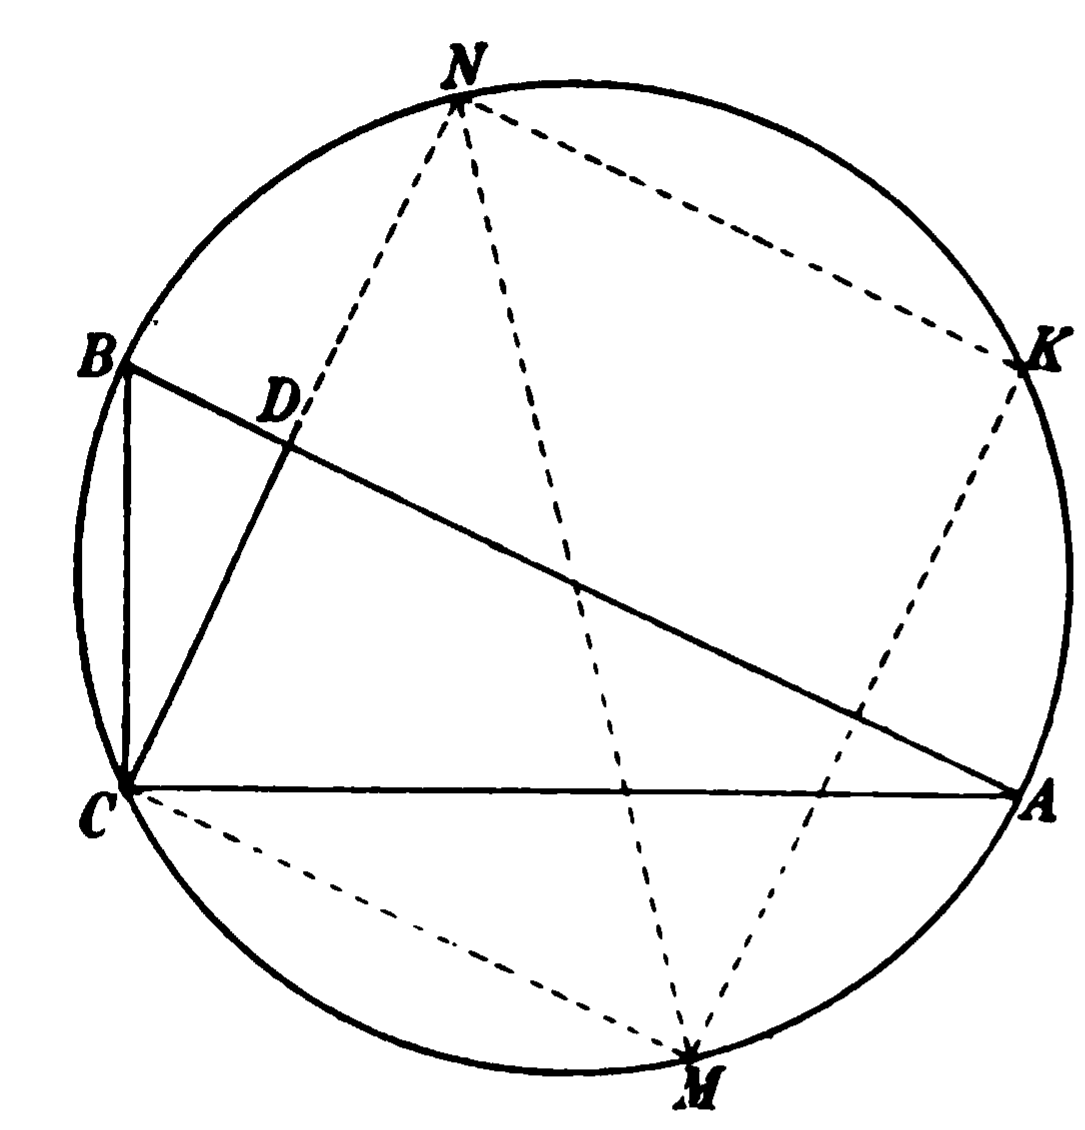
\includegraphics[width=\linewidth]{pdf244-right-triangle-construction.png}
\end{minipage}\hfill
\begin{minipage}[t]{0.57\textwidth}
(b) Let $ABC$ be a right triangle right-angled at $C$. Draw the perpendicular $CD$, dividing the hypotenuse into two parts $DB$ and $DA$. Produce $CD$ to meet the circum-circle again in $N$, and complete the inscribed rectangle $CNKM$ upon the side $CN$. Then $MNK$ is another right triangle, whose sides are $KN=DA-DB$ and $KM=2.CD$, the hypotenuse being the same as in the original triangle $ABC$. Now write $CB=(2m+1)$, $CA=(2n)$. Then we have
\end{minipage}
\[
2.CB.CA=AB(2.CD)=2(2m+1)(2n).
\]
Consequently the sides of the right triangle $KMN$ are proportional to
\[
(2n)^2-(2m+1)^2,\qquad 2(2m+1)(2n),\qquad (2n)^2+(2m+1)^2,
\]
which we take for the solution required.

(c) Take $c=(2m+1)^2+(2n)^2$, or souared
\[
c^2=(2m+1)^4+2(2m+1)^2(2n)^2+(2n)^4.
\]
If we here change the sign of $2(2m+1)^2(2n)^2$, the result is still a perfect square. Hence we may take $a=2(2m+1)(2n)$, for then we have
\[
c^2-a^2=\{(2m+1)^2+(2n)^2\}^2-4(2m+1)^2(2n)^2=\{(2m+1)^2-(2n)^2\}^2,
\]
so that $b=(2m+1)^2-(2n)^2$.

The values of $a$, $b$, $c$, that do not exceed 1000, are given in a table.

2. In the case of the scalene triangle, whose three sides and area are to be given in integral values, Matsunaga considers three ways, remarking that these are by no means very satisfactory and consequently desiring posterity to devise a simpler process.

(a) \emph{Kurushima's method}. Take the three fractions
\[
\frac{n_1}{d_1},\qquad \frac{n_2}{d_2},\qquad\text{and}\qquad
\frac{n_3}{d_3}=\frac{d_1d_2-n_1n_2}{n_1d_2+n_2d_1},
\]
\scanfooter

\scanpage{0245}{Chapter 32, printed page 231}
where the first two are selected at will. But it is remarked, the values of $d$ and $n$ such that $n_3<n_1$, $d_3<d_1$, or $n_3<n_2$, $d_3<d_2$, should not be used. If $n_3=n_1$, $d_3=d_1$, or $n_3=n_2$, $d_3=d_2$, the case will be of the isosceles triangle; and if $n_3=d_3-1$, the triangle will be right angled. Then
\[
a_1=n_1(n_2d_3+n_3d_2),\qquad a_2=n_2(n_3d_1+n_1d_3),\qquad a_3=n_3(n_1d_2+n_2d_1)
\]
give the values of the three sides of a triangle. If these values have factors common to them, such factors, it is remarked, should be removed.

The same rule of solution also applies, when the fractions $n_1/d_1$ and $n_2/d_2$ are reciprocated. In this case, if the product of the new denominators be less than that of the numerators, these values should not be adopted.

(b) \emph{A certain mathematician's method}. If we take three numbers $m$, $n$, $k$, where $m>n$, and form the quantities
\[
A=(m^2+n^2)k,\qquad B=(m^2+n^2)n\quad\text{or}\quad(n^2+k^2)m,
\]
\[
C=(m^2-n^2)k+(n^2-k^2)m\quad\text{or}\quad(m^2-n^2)k+(m^2-k^2)n,
\]
then any set of $A$, $B$, $C$ is a solution.

(c) \emph{Author's method}. Let $a_1$, $b_1$, $c_1$ and $a_2$, $b_2$, $c_2$ be any two sets of integral solutions of a right triangle, $c$ being the hypotenuse. Assume $a_1$, $a_2$ are odd, while $b_1$, $b_2$ are even. If we describe the right triangles with the common hypotenuse $c_1c_2$ and with the sides $a'_1=a_1c_2$, $b'_1=b_1c_2$, and $a'_2=a_2c_1$, $b'_2=b_2c_1$, and join the two vertices, we thus form the two triangles with the sides $a'_1$, $b'_2$ and $a'_2$, $b'_1$. By adjusting the two right triangles in different ways, eight such triangles will be formed in all. The third sides are $a_1a_2\pm b_1b_2$ and $a_1b_2\pm a_2b_1$. When the values of the three sides have a common factor, this is to be removed.

The actual values of the three sides below 1000 are given in a table, which is followed by another table giving the primitive numbers below 1000.

3. The equation $rx^2+y^2=z^2$ has the solution
\[
x=2mn,\qquad y=rm^2\mathord{\sim}n^2,\qquad z=rm^2+n^2,
\]
where $n$ is to be so selected that it does not contain the factor $r$, being even or odd according as $r$ is odd or even.

4. The solution of the equation $r(z^2-y^2)=x^2$ is
\[
x=2r\times mn,\qquad y=rm^2-n^2,\qquad z=rm^2+n^2.
\]
\scanfooter

\scanpage{0246}{Chapter 32, printed page 232}
5. Of the equations of the type $rx^2-y^2=z^2$, Matsunaga says some may be solved, while others remain without solution. In the types that have been solved $r$ is of the forms $k^2$, $2k^2$ or $k^2+l^2$.

(a) The solution of $2x^2-y^2=z^2$ is
\[
x=m^2+x^2,\qquad y=(m+n)^2-2n^2,\qquad z=(m+n)^2-2m^2.
\]

(b) The solution of $2k^2x^2-y^2=z^2$ is
\[
x=c,\qquad y=k(a\pm b),\qquad z=k(a\mp b),
\]
where $a$, $b$, $c$ are any integers satisfying the Pythagorean relation.

(c) The solutions of $(k^2+l^2)x^2-y^2=z^2$ are
\[
\begin{array}{r@{\qquad}l}
(1)&x=c,\qquad y=ka\pm lb,\qquad z=la+kb;\\[1mm]
(2)&x=c,\qquad y=la\mp kb,\qquad z=ka\pm lb,
\end{array}
\]
where $a$, $b$, $c$ are as before, and where the upper or the lower signs are to be simultaneously taken.

(d) The solution of $k^2x^2-y^2=z^2$ is $x=c$, $y=ka$, $z=kb$.

6. The equation of the type $kx^2-ly^2=z^2$, where $k-l$ is a perfect square, may be solved in some special cases. Thus, writing $x^2=\alpha^2+l\beta^2$, $y=\alpha+B\beta$, we have
\[
\begin{aligned}
z^2&=k\alpha^2-ly^2=k(\alpha^2+l\beta^2)-l(\alpha+B\beta)^2\\
&=(k-l)\alpha^2-2lB\alpha\beta+l(k-B^2)\beta^2\\
&=\frac1{k-l}\left\{[(k-l)\alpha-lB\beta]^2+[(k-l)l(k-B^2)-l^2B^2]\beta^2\right\},
\end{aligned}
\]
which is to be made a perfect square. This may be realised if we write $(k-l)l(k-B^2)-l^2B^2=0$, whence $B$ may be determined to be $B=\pm\sqrt{k-l}$. Thus the values of $y$ and $z$ become
\[
y=\alpha\pm\sqrt{k-l}\,\beta,\qquad z=l\beta\pm\alpha\sqrt{k-l}.
\]
Now the values of $\alpha$ and $\beta$ should be so determined as to satisfy the relation $x^2=\alpha^2+l\beta^2$. Hence from § 3 we have
\[
x=lm^2+n^2,\qquad \alpha=lm^2-n^2,\qquad \beta=2mn.
\]
Again similarly writing $y^2=\alpha^2-k\beta^2$, $x=\alpha+B\beta$, we obtain
\[
x=(km^2+n^2)\pm\sqrt{k-l}(2mn),\qquad y=km^2-n^2,
\]
\[
z=\sqrt{k-l}(km^2+n^2)\pm k(2mn).
\]

7. The equation $k^2x^2-ry^2=z^2$ or $rx^2-k^2y^2=z^2$ may be solved by applying to the cases we have already explained. But the general equation of the type $kx^2-ry^2=z^2$, where neither $k-r$, nor $k$ nor $r$ is a perfect square is mentioned by Matsunaga as not yet solved.
\scanfooter

\scanpage{0247}{Chapter 32, printed page 233}
8. To solve the equation $kx^2+ry^2=z^2$, where $k+r$ is a perfect square, Matsunaga applies a similar method as above, writing
\[
y^2=\alpha^2-k\beta^2,\qquad x=\alpha+B\beta;
\]
or
\[
x^2=\alpha^2-r\beta^2,\qquad y=\alpha+B\beta.
\]

9. The solution of the equation $x^2+xy+y^2=z^2$ is given to be
\[
x=m^2-n^2,\qquad y=(m+n)^2-m^2,\qquad z=(m+n)^2-mn.
\]
When the sign of $xy$ is negative, the expressions for $y$ and $z$ should be exchanged.

10. To solve the equation $x^2+y^2+z^2=u^2$, Matsunaga takes $x$ and $y$ at pleasure; then $x^2+y^2$ being separated into the product of two factors $\alpha$ and $\beta$, the values of $z$ and $u$ will be given by
\[
z=\frac12(\alpha\mathord{\sim}\beta)\qquad\text{and}\qquad u=\frac12(\alpha+\beta).
\]
This consideration will apply to the case of the equation
\[
x_1^2+x_2^2+\cdots=y^2,
\]
though it is not mentioned by the author.

11. The solution of the equation $x^2+y^2=z^3$ is
\[
x=(m^2\mathord{\sim}3n^2)m,\qquad y=(3m^2\mathord{\sim}n^2)n,\qquad z=m^2+n^2.
\]

12. The solution of $x^3+y^3+z^2=u^4$ is
\[
x=m^4-n^4,\qquad y=4m^2n^2,\qquad z=2(m^2-n^2)mn,\qquad u=m^2+n^2.
\]
Here the author adds that there has been found no method applicable to the case of more than four elements.

13. The solution of $x^2-y^2=z^4$ is
\[
x=m^4-n^4,\qquad z=m^2-n^2,\qquad y=2mnz.
\]

14. Equation $x^3-y^3=z^4$: solution
\[
z=m^3-n^3,\qquad x=zm,\qquad y=zn.
\]

15. To solve the equation $x^2+y^2=k$, let $\frac12k=r^2+R$, where $r^2$ is the greatest square contained in $k$. Form the quantities
\[
a_1=2r-1,\qquad a_2=a_1-2,\qquad a_3=a_2-2,\qquad a_4=a_3-2,\ldots,
\]
\[
b_1=2r+1,\qquad b_2=b_1+2,\qquad b_3=b_2+2,\qquad b_4=b_3+2,\ldots,
\]
and from $2R=A$ successively subtract $b_1$, $b_2$, \ldots. When these subtractions are impossible, successively add $a_1$, $a_2$, \ldots\ and carry out the subtractions. If we come at last to a remainder that vanishes, let the values of $a$ and $b$ employed in the last place be $a'$ and $b'$. Then
\[
x=\frac12(a'+1)\qquad\text{and}\qquad y=\frac12(b'-1)
\]
is a solution required.
\scanfooter

\scanpage{0248}{Chapter 32, printed page 234}
Another solution. Let $k=r'^2+R'$, and write
\[
a'_1=2r'-1,\qquad a'_2=a'_1-2,\qquad a'_3=a'_1-4,\qquad a'_4=a'_1-6,\ldots.
\]
From $R$ subtract successively $1$, $3$, $5$, \ldots, until it becomes impossible to carry on the operation any more. Let the last remainder be $A'$ and the last subtrahend be $b'_1$. Write
\[
b'_2=b'_1+2,\qquad b'_3=b'_1+4,\qquad b'_4=b'_1+6,\ldots,
\]
and proceed as in the first way. Thus we may similarly obtain the required values of $x$ and $y$.

16. To solve the equation $a^2+bx=y^2$, separate $b$ into the product of two factors $mn$ and find a number $p$ that satisfies the relation $mp-nq=1$. Find a number $A$ such that $2pa\equiv A\pmod n$. Then $x=\frac1nA(Am-2a)$ will be a value required. If $Am-2a$ be $=0$, then $A+n$ should be taken in place of $A$ and we proceed in the same manner. If $A=0$, take $m$ for $A$. If $Am-2a<0$, we have to take $(A+1)m-2a$ in place of $Am-2a$.

Or otherwise. If we write $2a+b$ in the form $bQ+R$, then $x=(2a+b)-(Q+1)R$ will be an answer. It is here noted that this will be advantageously applied when $b$ is a prime number. It will lead, however, in the contrary case, to a value of $x$ which is not very small.

17. To solve the equation $a+bx=y^2$, for example $69+11x=y^2$, we have first to form the quantities
\[
1=1^2\equiv\alpha_1,\qquad 1+3=2^2\equiv\alpha_2,\qquad 1+3+5=3^2\equiv\alpha_3,\ldots
\]
with the modulus $b=11$. The number of $\alpha$'s is evidently restricted to a certain number. In our case we have only to take $\alpha_1=1$, $\alpha_2=4$, $\alpha_3=9$, $\alpha_4=5$, $\alpha_5=3$. We have then
\[
\frac ab=Q+\frac Rb=6+\frac3{11},
\]
and comparing $R=3$ with the $\alpha$'s, we see that $R$ is equal to $(\alpha_r=)\alpha_5$. If there is no $\alpha$ which is equal to $R$, the problem is insoluble. Now form the quantities
\[
2\times r+b=21=1\times b+10=Q'b+R',
\]
\[
(2r+b)-(Q'+1)R''=1=K,\qquad Kb+r^2=36=6^2=k^2,
\]
\[
k+b=23=bQ''+R''=b\times2+1,
\]
\scanfooter

\scanpage{0249}{Chapter 32, printed page 235}
\[
(k+b)-(Q''+1)R''=23-3\times1=20=h,
\]
\[
h\times b+k^2=256,\footnote{If this quantity be $<a$, a further procedure is required to be repeated as already done.}\qquad \frac{256-a}{b}=17,
\]
and this last quantity is a required value of $x$.

18. ``\emph{Problem}. There is a certain number as yet unknown. If we evolve it in the second degree with 69 as the additive 1st degree coefficient, there will remain the remainder 15. If we do the same with the additive quantity 72, the remainder will be 7. What is the unknown number?''

As we have here translated literally the meanings of the technical terms employed, it will be hardly intelligible to any reader who is not familiar with the peculiar mode of writing of the old Japanese mathematicians. But if we symbolically represent, the problem is nothing but to find the integral number value of $x$ satisfying the equations:
\[
y_1^2+69y_1=x-15,\qquad y_2^2+72y_2=x-7,
\]
or generally
\[
y_1^2+a_1y_1=x-b_1,\qquad y_2^2+a_2y_2=x-b_2.
\]
Matsunaga solves this problem thus: Factorise the quantity
\[
(a_2^2+4b_1)\mathord{\sim}(a_1^2+4b_2)=455
\]
into $mn$, whereby $m$ and $n$ should be so chosen that $m+n\geq2a_1$ or $2a_2$. In our case, therefore, the two factors 91 and 5 are not to be taken, and so we have to take $m=455$ and $n=1$. We have then
\[
\frac12\left(\frac{m-n}{2}-a_1\right)=79=y_1,
\qquad
\frac12\left(\frac{m+n}{2}-a_2\right)=78=y_2,
\]
and the value of $x$ follows directly to be 11707.

In case $\frac12(m-n)-a_1<\frac12(m+n)-a_2$, we have to take
\[
y_1=\frac12\left(\frac{m+n}{2}-a_1\right),
\qquad
y_2=\frac12\left(\frac{m-n}{2}-a_2\right).
\]
The analysis of this rule is tried thus: Eliminating $x$ from the two given relations we have
\[
(-b_2+b_1+a_1y_1+y_1^2)-a_2y_2-y_2^2=0,
\]
from which follows
\[
y_2=-\frac{a_2}{2}+\frac12\sqrt{a_2^2+4(-b_2+b_1+a_1y_1+y_1^2)}.
\]
Here expressing the quantity under the radical sign by $k_2^2$, and solving it for $y_1$, it follows (whereby we use the letter $l$)
\[
y_1=-\frac{a_1}{2}+\frac12\sqrt{a_1^2+4b_2-a_2^2-4b_1+k_2^2}
=-\frac{a_1}{2}+\frac12l.
\]
\scanfooter

\scanpage{0250}{Chapter 32 continuation, printed page 236}
Now let the numerical value of $a_1^2+4b_2-a_2^2-4b_1$ be equal to $\pm mn$. Then in order that $l^2$ should be a perfect square, $l$ must be of the form $\frac12(m\pm n)$. Hence we have
\[
y_1=\frac12\left(\frac{m\pm n}{2}-a_1\right),
\qquad\therefore\qquad
k^2=\left(\frac{m\pm n}{2}\right)^2\mp mn=\left(\frac{m\mp n}{2}\right)^2,
\]
and therefore $y_2$ has the value
\[
\frac12\left(\frac{m\mp n}{2}-a_2\right).
\]

19. To solve the equation $a+cx=(b+dx)y$, Matsunaga rewrites it in the form $(a-by)+(c-dy)x=0$ and considers it as an equation in $x$. If the coefficient of $x$ be free from any unknown quantity, the \emph{jōichi jutsu} or the relation $mp-nq=1$ may be applied. If the absolute term be free from any unknown quantity, we may solve it by factorising this term. But in the case before us both the coefficient of $x$ and the absolute term are dependent on $y$, which is yet unknown, and thus neither of the two is directly applicable. If however we write $x=x_1/d$ the equation becomes
\[
(ad-bdy)+(c-dy)x_1=0,
\]
and making the substitution $x_1=x_2-b$ we get
\[
(ad-bd)+(c-dy)x_2=0,
\]
thus leading to a form in which the absolute term is independent of $y$. Since $x$ is to be positive, $x_1$ must also be so, and consequently $x_2-b>0$, or $x_2>b$ and necessarily positive. Hence the two coefficients of the last form of the equation are of different signs. Then we shall write it in the form
\[
mn\pm(c-dy)x_2=0,
\]
where the two signs depend on circumstances. We have now only to take $m=x_2$, $n=\mp(c-dy)$, which ought to be necessarily positive. The values of $x$ and $y$ follow at once.

20. In what we have described in the above, the factorization of a number has been often resorted to. Matsunaga's trial of the matter is something as follows: Let a number to be factorised be written in the form $r^2+R$ and we shall first consider the case of $r$ odd. Now writing
\[
r=B_1,\qquad B_1-2=B_2,\qquad B_2-2=B_3,\qquad B_3-2=B_4,\ldots,
\]
the following calculations will be made:
\[
\begin{array}{rcl@{\qquad}rcl@{\qquad}rcl}
R&=&Q_1B_1+A_1,&K_1&=&2Q_1,&K'_2&=&K_1+4,\\
A_1+K'_2&=&Q_2B_2+A_2,&K_2&=&2Q_2+K'_2,&K'_3&=&K_2+8,\\
A_2+K'_3&=&Q_3B_3+A_3,&K_3&=&2Q_3+K'_3,&K'_4&=&K_3+8,\\
A_3+K'_4&=&Q_4B_4+A_4,&K_4&=&2Q_4+K'_4,&K'_5&=&K_4+8,
\end{array}
\]
\[
\cdots\cdots\cdots\cdots\cdots\cdots\cdots\cdots\cdots
\]
\scanfooter


\scanpage{0251}{Chapter 32 conclusion and Chapter 33, printed page 237}
which will come to an end, when we arrive at a vanishing value of $A_n$. In this case the value of $B_n$ is a required factor. The other factor will be given by $\frac12K_n+B_n+2$.

In case $r$ is even, we have to write $r-1=B_1$ and to take $R+1$ in place of $R$, and proceed in the same manner as in the other case.

In these calculations labour may be saved by abbreviating two or three steps in a single operation, which will easily follow.

\begin{center}
CHAPTER 33.\\[1mm]
THE INDETERMINATE EQUATION $x^n-ky=a$.
\end{center}
\phantomsection\addcontentsline{toc}{subsection}{Chapter 33. The Indeterminate Equation $x^n-ky=a$}

There is an anonymous manuscript probably, or certainly, belonging to the first part of the 18th century entitled \emph{Ruijō Ruiyaku Shinjutsu}, in which the indeterminate equation $x^n-ky=a$ is solved. For that purpose the unknown author forms the congruences:
\[
1^n\equiv1\equiv a_1,\qquad 2^n\equiv a_2,\qquad 3^n\equiv a_3,\ldots,\qquad (k-1)^n\equiv a_{k-1},
\]
for the modulus $k$. Then selecting from among the quantities $a_1,a_2,\ldots,a_{k-1}$ that which is equal to the given number $a$, let it be $a_r$. The author now takes $x=r$ to be the required value of $x$.

In forming the above congruences a considerable amount of labour may be saved by some contrivances. Thus we see that $a_{k-r}=a_r$ or $k-a_r$, according as $k$ is even or odd. This may be proved as follows:\footnote{Here we write $(M)$ to mean ``a multiple of''.}
\[
\begin{aligned}
(k-r)^n&=(M)k+(-1)^nr^n=(M)k+(-1)^n\{(M)k+a_r\}\\
&=(M)k+(-1)^na_r=(M)k+a_r\quad\text{or}\quad(M)k+(k-a_r).
\end{aligned}
\]
Again in finding $a_r$ it is not necessary to form the $n$th power of $r$. For we may advantageously proceed thus:
\[
r^2\equiv b_1,\qquad r^3\equiv b_1r\equiv b_2,\qquad r^4\equiv b_2r\equiv b_3,\ldots,\qquad r^n\equiv b_{n-2}r\equiv a_r.
\]
When $r$ is of the form $r_1r_2r_3\cdots$, we may employ the residues of the factors, whose product affords the required residue of $r$.

For example we take the equation $x^5-29y=25$. Here we have for $a_1,a_{28};a_2,a_{27};\ldots$ the following values:
\[
\begin{array}{rrrrrrrrrrrrrr}
1&3&11&9&22&4&16&27&5&8&14&12&6&19\\
28&26&18&20&7&25&13&2&24&21&15&17&23&10
\end{array}
\]
In this table we see that the number 25 is given by $a_{23}$. The required value of $x$ is, therefore, $x=23$.
\scanfooter

\scanpage{0252}{Chapter 34 opening, printed page 238}
\begin{center}
CHAPTER 34.\\[1mm]
AJIMA'S \emph{RENJUTSU HENKAN}.
\end{center}
\phantomsection\addcontentsline{toc}{subsection}{Chapter 34. Ajima's Renjutsu Henkan}

In the 3rd month of 1784 Ajima Chokuyen wrote the manuscript entitled \emph{Renjutsu Henkan}. This title may be probably rendered in ``The adaptation of general considerations to cases of similar nature''. It was one of the results representing the highest mark of development of the \emph{tenzan} algebra. The contents of the book are essentially as reproduced in the following lines.

\begin{center}
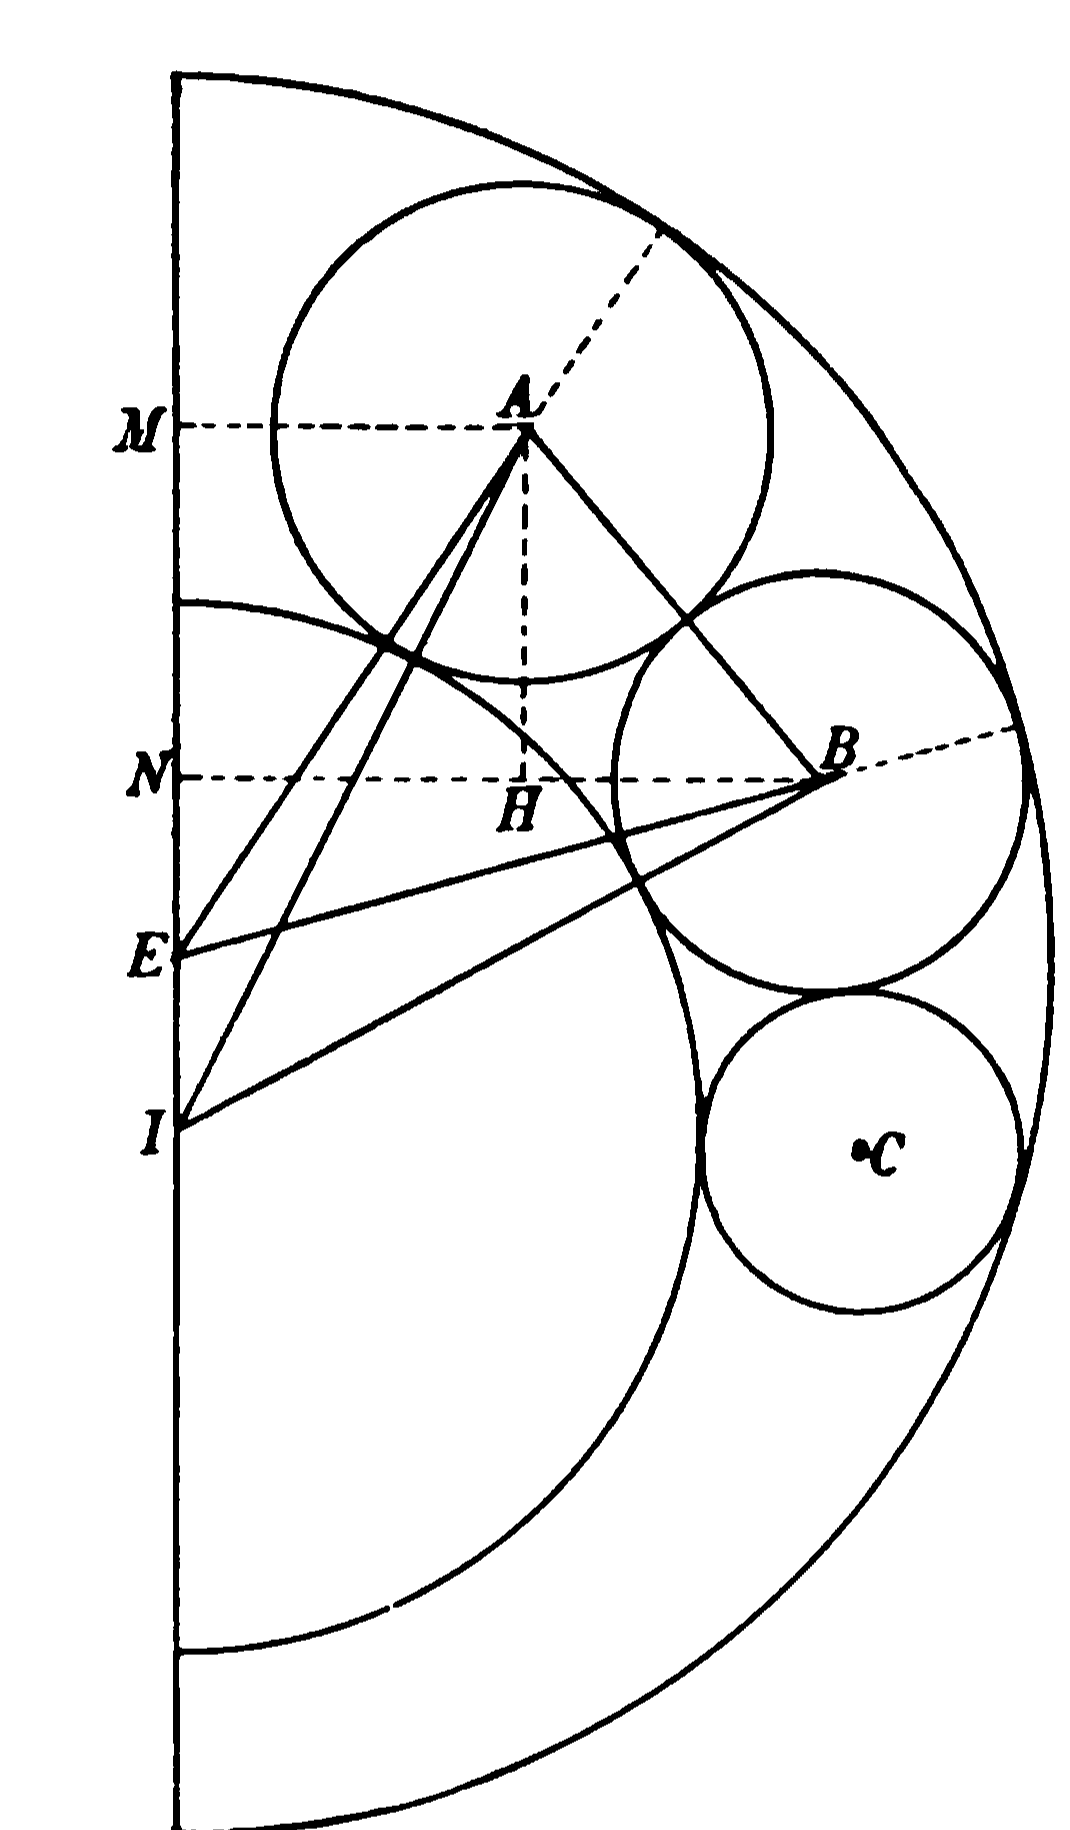
\includegraphics[width=0.48\linewidth]{pdf252-renjutsu-three-circles.png}
\end{center}

1. In the figure let $E$ be the external circle and $I$ the internal circle. Three circles $A,B,C$ are described touching these two circles and one another. We denote by these letters the centres of the respective circles as well as their diameters. It is required to find $A$ and $C$ in terms of $I,E,B$, and the sagitta $s$, which is the part of the common diameter of $E$ and $I$ comprised between the two circumferences.

We write
\[
\begin{gathered}
a=2\dd\overline{IE}=-E+I+2s,\qquad b=2\dd\overline{EA}=E-A,\\
c=2\dd\overline{IA}=I+A,\qquad d=2\dd\overline{EB}=E-B,\\
e=2\dd\overline{IB}=I+B,\qquad f=2\dd\overline{AB}=A+B,
\end{gathered}
\]
and drawing $AM$ and $BN$ at right angles to $IE$, and $AH$ to $BN$, we write $g=2\dd EM$, $h=AM$, $i=2\dd EN$, $j=BN$, $k=2\dd AH$, $l=BH$. We have then\footnote{The expressions in the text are not very trustworthy, being different in different transcripts. I have not, however, necessarily tried to correct them, for my aim will be attained if the main feature of the analysis could be represented.}
\[
ag=\frac12(c^2-a^2-b^2),\qquad\text{and}\qquad a^2h^2=\frac14(a^2b^2-a^2g^2),
\]
or effecting reduction and writing $m=E\dd I+Es-Is-s^2$, we get
\[
a^2h^2=m\{(E-I)s+s^2+(E-I)A-A^2\}.
\]
We have similarly
\[
a^2j^2=m\{-(E-I)s+s^2+(E-I)B-B^2\},
\]
\scanfooter

\scanpage{0253}{Chapter 34, printed page 239}
and further
\[
a^2l^2=m(-A^2+2AB-B^2)+(E+I)AB,
\]
\[
\begin{aligned}
a^2j\times2l&=a^2l^2+a^2j^2-a^2h^2\\
&=m\{-2AB-2B^2-(E-I)A+(E-I)B\}+(A+B)^2AB.
\end{aligned}
\]
Now equating the square of $a^2j^2\times2l$ with 4 times the product of $a^2j^2$ and $a^2l^2$, we have, after rearrangement and the removal of the factor $a^2$, the equation
\[
\alpha\equiv
\left\{
\begin{aligned}
&\{(I+E)^2B^2+m^2-2m(E-I)B\}x^2\\
&+\{-2m(E-I)B^2-2mnB+2m(E-I)Bs\}x+m^2B^2
\end{aligned}
\right\}=0,
\]
from which $A$ is to be determined. Here we have written $n=EI+s^2$. If we change $A$ into $B$ and $B$ into $C$, we obtain the equation for $C$. But by these changes the equation remains unchanged. Hence $A$ and $C$ are the two roots of the above equation.

If we write
\[
\beta=\{(E-I)B+n-(E-I)s\}x-mB,
\]
we have\footnote{For it is $\alpha=0$.}
\[
\beta^2=\beta^2-\alpha=\{4IE(B+s)(B-s)-4IE(E-I)(B-s)\}x^2.
\]
Consequently designating the coefficient of $x^2$ in the right-hand side by $\gamma^2$ and taking the square roots of both sides we get
\[
\{(E-I)B+n-(E-I)s\mp\gamma\}x-mB=0,
\]
where the upper sign pertains to $A$ and the lower to $C$.

From these two expressions for $A$ and $C$, by multiplying $C$ and $A$ respectively and adding together, we get
\[
\{-mB+2(E-I)BC+2nC-2(E-I)sC\}x-mBC=0,
\]
which serves to give $A$ in terms of $B$ and $C$. This is called the fundamental equation.

2. Next Ajima proceeds to find the diameters of the circles $A_2,A_3,\ldots$, which are described as shown in the figure, in terms of $E,I$ and $A_1$.

\begin{center}
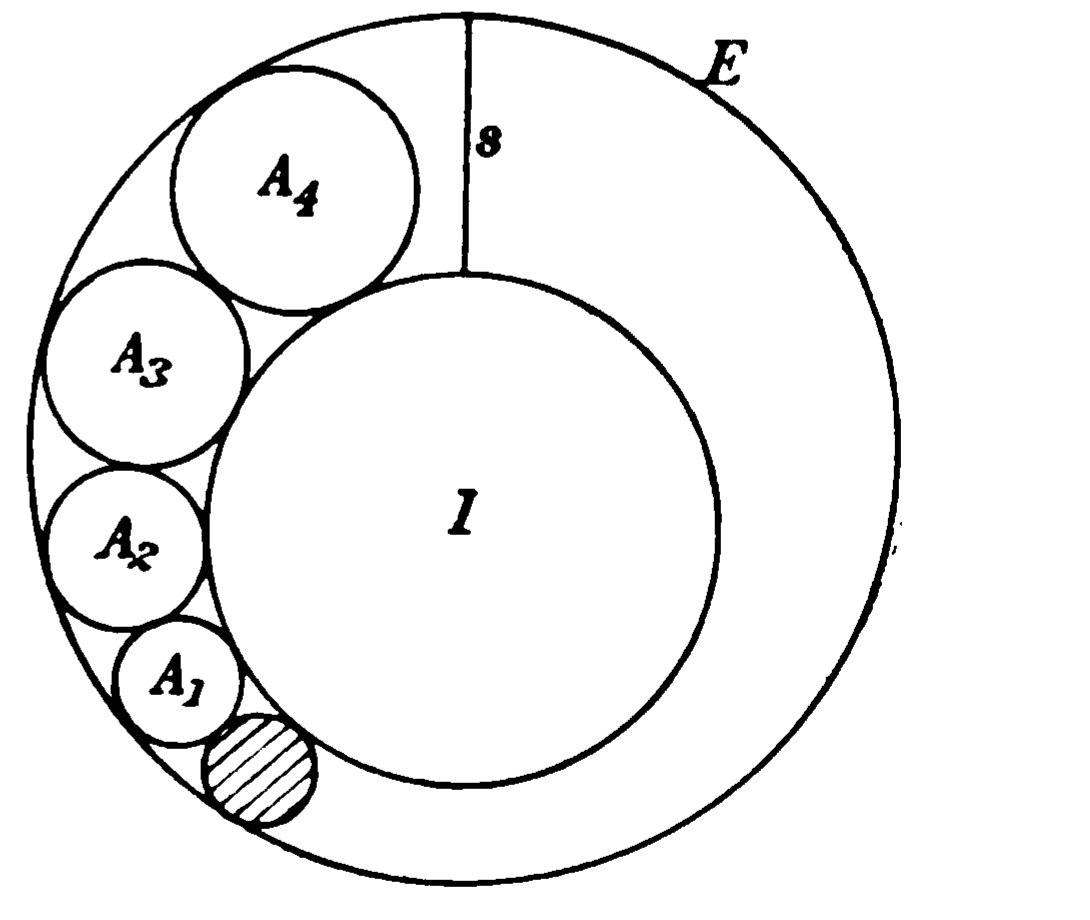
\includegraphics[width=0.40\linewidth]{pdf253-successive-circles.png}
\end{center}

Here the coloured circle corresponds to the circle $C$, and the circles $A_1$ and $A_2$ to $B$ and $A$ of the case already considered. And thus from the relation we have obtained we get, for $x=A_2$,
\[
\{(E-I)A_1+2EI-m-p\}x-mA_1=0,
\]
\scanfooter

\scanpage{0254}{Chapter 34, printed page 240}
where we write
\[
m=IE+Es-Is-s^2=(E-s)(I+s),
\]
\[
p=2\sqrt{(A_1+s)(A_1-s)IE-(E-I)(A_1-s)IE}.
\]
Again substituting in the fundamental equation $A_1$ for $C$ and $A_2$ for $B$, we obtain
\[
\{-mA_2+2(E-I)A_1A_2+2nA_1-2(E-I)sA_1\}x-mA_1A_2=0,
\]
from which $x=A_3$ is to be determined. Here $n$ denotes $EI+s^2$. This equation may be written in the form
\[
\left\{-1+\frac{2(E-I)A_1}{m}+\frac{4EIA_1}{A_2m}-\frac{2A_1}{A_2}\right\}x-A_1=0,
\]
which is called the second fundamental equation.

If we write
\[
\frac{A_1}{A_1}=1=\rho_1,\qquad \frac{A_1}{A_2}=\rho_2,\qquad \frac{A_1}{A_3}=\rho_3,\ldots,
\]
this equation becomes
\[
(-\rho_1+\rho+\rho_2k)x-A_1=0,
\]
where
\[
k=\frac{4EI}{m}-2,\qquad \rho=\frac{2(E-I)A_1}{m},
\]
and hence
\[
\rho_3=\rho_2k+\rho-\rho_1,\qquad\text{and}\qquad A_3=A_1/\rho_3.
\]
If we substitute $A_2$ for $A_1$ and $A_3$ for $A_2$ in the second fundamental equation we obtain the equation for $A_4$ in the form
\[
\left\{-1+\frac{2(E-I)A_2}{m}+\frac{4EIA_2}{mA_3}-\frac{2A_2}{A_3}\right\}x-A_2=0,
\]
which is called the third fundamental equation. By multiplying with $\rho_2$, this transforms into
\[
\left\{-\rho_2+\frac{2(E-I)A_1}{m}+\frac{4EIA_1}{A_3m}-\frac{2A_1}{A_3}\right\}x-A_1=0,
\]
or
\[
(-\rho_2+\rho+k\rho_3)x-A_1=0,
\]
whence we get
\[
\rho_4=\rho_3k+\rho-\rho_2,\qquad\text{and}\qquad A_4=A_1/\rho_4.
\]
Proceeding in this way the values of $\rho_5,\rho_6,\ldots$ may be successively obtained. Thus
\[
\rho_i=\rho_{i-1}k+\rho-\rho_{i-2},\qquad\text{and}\qquad A_i=A_1/\rho_i.
\]
This relation may be proved by mathematical induction but no such method of proof was possessed of by the old Japanese mathematicians. In cases like this it was only customary to take the relation for granted from its existence in a few first instances.
\scanfooter

\scanpage{0255}{Chapter 34, printed page 241}
3. When $A_1$ agrees with $s$, we have $\rho_1=1$, and
\[
1\times k+\rho-\rho_2=\rho_2,
\qquad \therefore\quad \rho_2=\frac{k+\rho}{2};
\]
and the same formulae for $\rho_3,\rho_4,\ldots$ apply as given above.

4. When the circle $A_1$ touches $s$, the diameter $A_1$ is first to be found from the equation
\[
(E+I)^2x^2-4m(E-I)x+(4m^2-4mEI)=0,
\]
which is obtained from the quadratic for $A$ in terms of $B$ in \S~1.

5. Ajima's consideration is not necessarily restricted to the simple case where the internal circle entirely lies within the external circle. He even takes up the case where the ``internal'' circle, that intersects the ``external'' circle, becomes infinitely great. He says thus:

``When the internal circle increases in magnitude without limit, its circumference gradually stretches itself until at last it becomes a straight line. In that case the length of the diameter of the internal circle is not measurable by our means; there is no bound to its magnitude. The figure of this case is as annexed. This figure is that of a circular segment, whithin which a series of successive circles are inscribed, and now the problem reduces to that of finding the diameters of these circles in terms of the external diameter $E$, the sagitta $s$ and the diameter of the circle $A_1$.''

\begin{center}
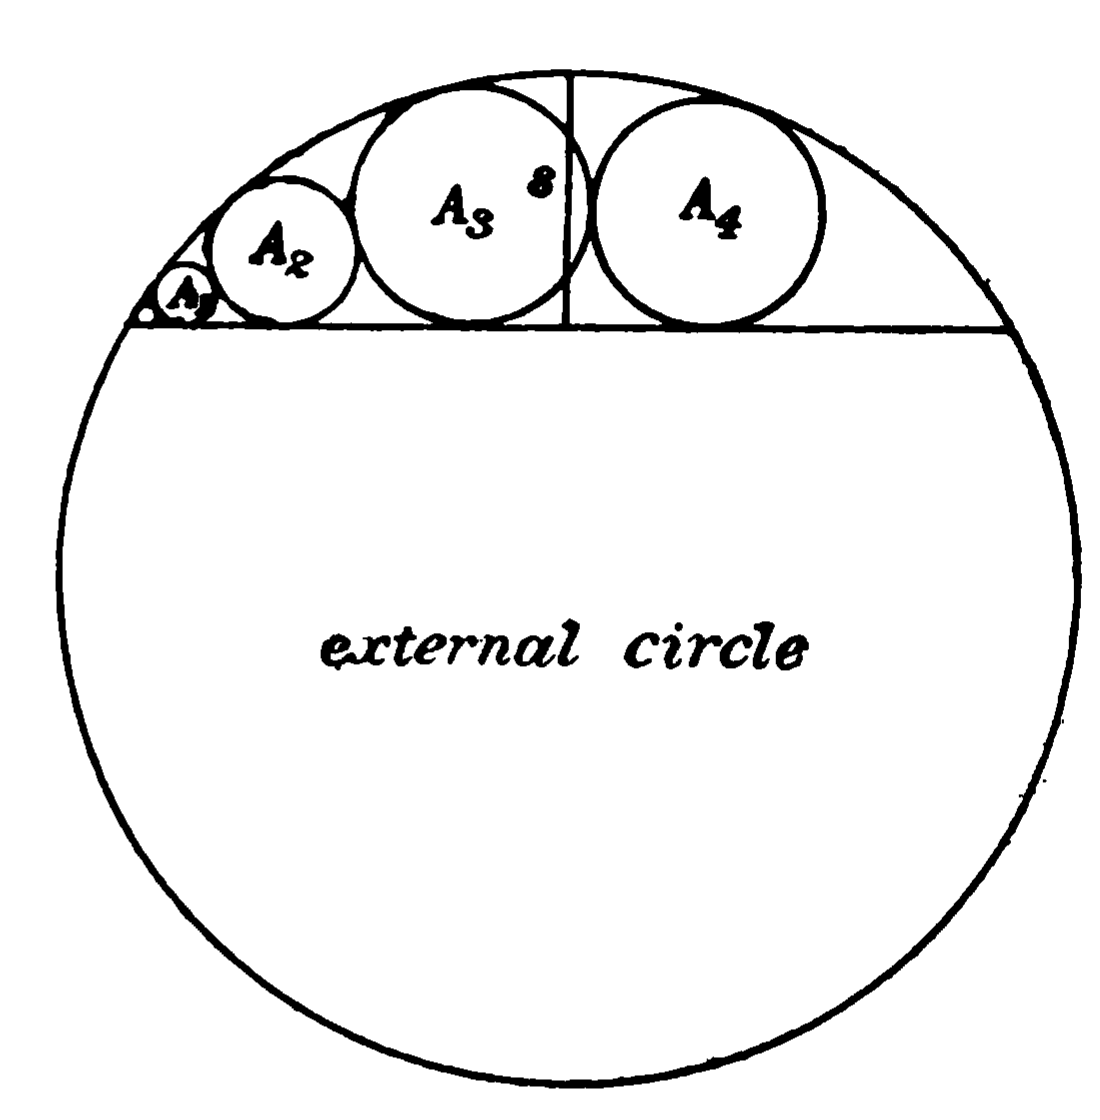
\includegraphics[width=0.44\linewidth]{pdf255-segment-inscribed-circles.png}
\end{center}

As Ajima considers, here we have
\[
m=(E-s)(I+s),\qquad k=\frac{4EI}{(I+s)(E-s)}-2,\qquad \rho=\frac{2(I-E)A_1}{(I+s)(E-s)},
\]
and consequently in the limit $I=\infty$ we have
\[
m=(E-s)\times(\text{infinity}),\qquad k=\frac{4E}{E-s}-2,\qquad \rho=\frac{2A_1}{E-s}.
\]
Now to find $\rho_2$, Ajima takes the equation obtained in \S~1,
\[
\{(I+E)^2B^2+m^2-2m(E-I)B\}A^2
+\{-2m(E-I)B^2-2mnB+2m(E-I)Bs\}A+m^2B^2=0,
\]
and writes in it $A=A_1$, $B=A_2$, replaces $m$ and $n$ by their values and divides by $(I+E)^2$ and goes to the limit $I=\infty$, when the result is
\[
\begin{aligned}
&A_1^2A_2^2+2(E-s)A_1^2A_2+2(E-s)A_1A_2^2-2(E-s)sA_1A_2\\
&\qquad{}-2(E-s)EA_1A_2+(E-s)^2A_1^2+(E-s)^2A_2^2=0,
\end{aligned}
\]
\scanfooter

\scanpage{0256}{Chapter 34, printed page 242}
which is called the equation for the circle inscribed in a segment. This is quadratic in $A_2$ and treating as done in \S~1, we get
\[
\{-A_1+E+s\mp\sqrt{E(s+A_1)}\}x-(E-s)A_1=0,
\]
where the upper sign pertains to $A_2$ and the lower to the circle on the other side of $A_1$. Dividing by $E-s$, for $A_2$ we have
\[
\frac1{E-s}\{-A_1+E+s-2\sqrt{E(s+A_1)}\}x-A_1=0,
\]
whence we obtain the value of $\rho_2$. In similar way as we have done before, the quantities $\rho_3,\rho_4,\ldots$ may be obtained and with them the values of $A_2,A_3,A_4,\ldots$.

6. The cases where the circle $A_1$ is described about the sagitta $s$ as diameter or where $A_1$ touches the sagitta of the segment may be treated as special cases from the general formulae obtained in the last paragraph.

7. When the external and internal circles touch each other we have
\[
s=E-I,\qquad E-s=I,\qquad I+s=E,\qquad m=IE,\qquad n-(E-I)s=IE,
\]
so that the equation of $A_2$ becomes
\[
\{I^2E^2-2(E-I)IEA_1+(E+I)^2A_1^2\}x^2
+\{-2I^2E^2A_1-2(E-I)IEA_1^2\}x+I^2E^2A_1^2=0,
\]
solving which we get
\[
\left\{1+\frac{(E-I)A_1}{EI}-\sqrt{\frac{4(E-I)A_1}{EI}-\frac{4A_1^2}{EI}}\right\}x-A_1=0,
\]
whence the coefficient of $x$ gives the value of $\rho_2$. For $\rho$ and $k$ we have
\[
\rho=\frac{2(E-I)A_1}{m}=\frac{2(E-I)A_1}{IE},\qquad k=\frac{4IE}{m}-2=2,
\]
which serve for the determination of the values of $\rho_3,\rho_4,\ldots$.

8. Suppose the external circle in the case just considered becomes infinitely great. In this case the external circle stretches out into a straight line. Here $A_1$ is necessarily greater than $A_2$, so that we adopt the equation
\[
\left\{1+\frac{(E-I)A_1}{EI}+\sqrt{\frac{4(E-I)A_1}{EI}-\frac{4A_1^2}{EI}}\right\}x-A_1=0
\]
for the determination of $A_2$, taking the positive sign before the radicand. When we go to the limit $E=\infty$, this becomes
\[
\left(1+\frac{A_1}{I}+\sqrt{\frac{4A_1}{I}}\right)x-A_1=0,
\]

\begin{center}
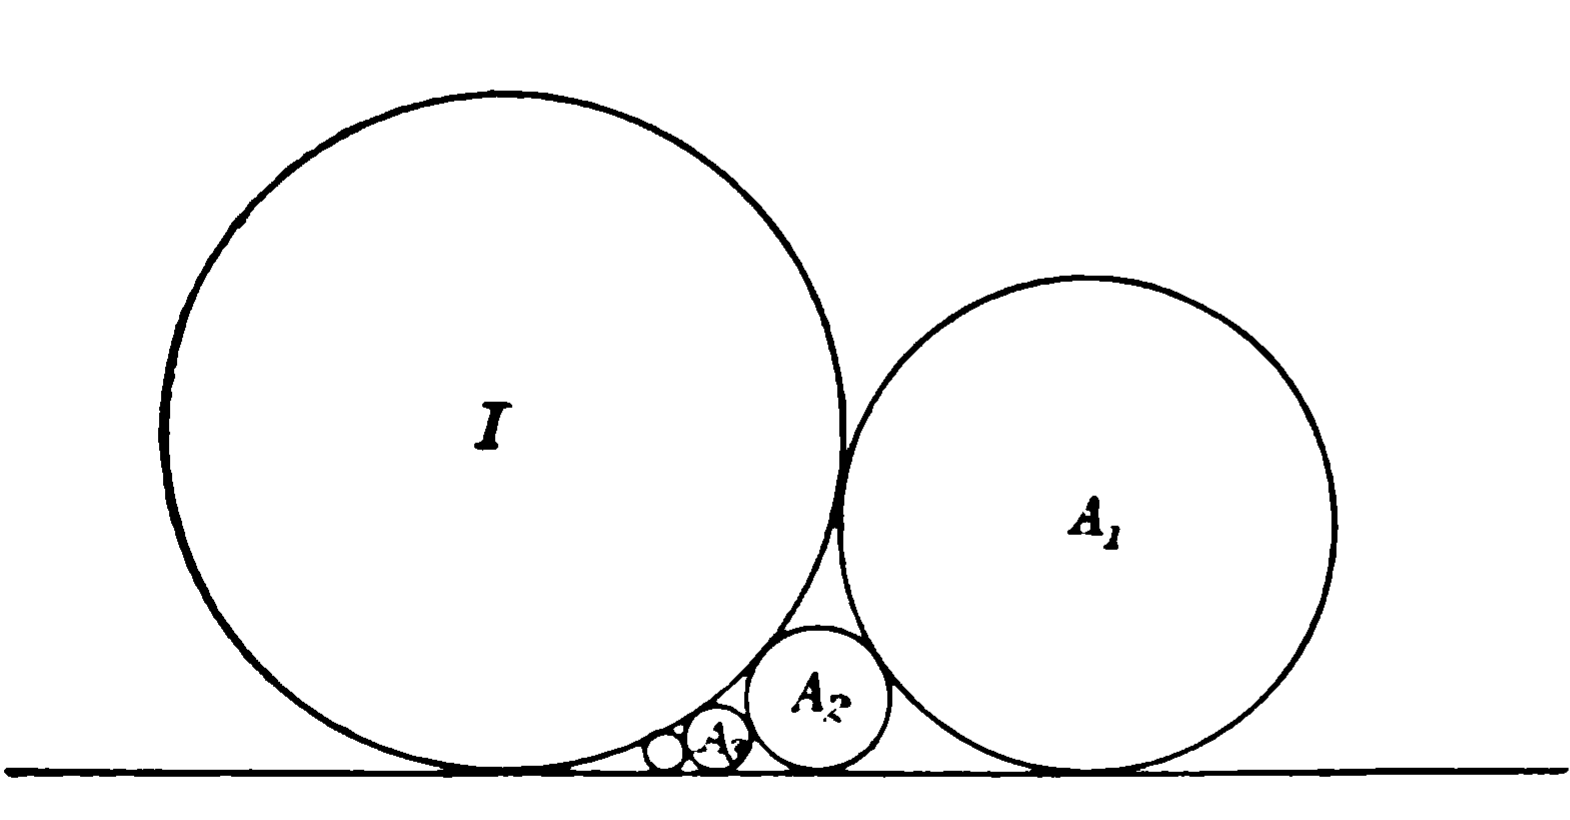
\includegraphics[width=0.56\linewidth]{pdf256-line-tangent-successive-circles.png}
\end{center}
\scanfooter

\scanpage{0257}{Chapter 34 conclusion and Chapter 35 opening, printed page 243}
whence we obtain $\rho_2$ and $A_2$. Now $\rho$ and $k$ are of the values
\[
\rho=\frac{2(E-I)A_1}{EI}=\frac{2A_1}{I},\qquad k=2,
\]
and serve for determining the values of $\rho_3,\rho_4,\ldots$.

9. Ajima concludes the work with these words: ``Besides what we have considered in the foregoing treatise, we may proceed in similar way whenever we meet with a class of problems whose natures resemble each other, by first discussing the general case and then changing the result for like cases. Here we have selected only a case of the \emph{renjutsu} and discussed it for example's sake.''

Thus it appears Ajima had meant by the term \emph{renjutsu} the general consideration that may be applied to special cases. The considerations of the old Japanese mathematicians are generally believed to have ever been of special nature and to have lacked in generality, but when we come to examine the contents of the manuscript before us, we feel that such a belief does not apply to the case of the gifted Ajima Chokuyen, who was particularly noted for his creative genius.

\begin{center}
CHAPTER 35.\\[1mm]
AJIMA'S STUDY OF CIRCLES SUCCESSIVELY INSCRIBED\\
FORMING A CROWN WITHIN A CIRCLE.
\end{center}
\phantomsection\addcontentsline{toc}{subsection}{Chapter 35. Ajima's Study of Circles Successively Inscribed Forming a Crown Within a Circle}

1. Mention has been made in the last chapter of Ajima's studies of the circles successively inscribed between two circles, external and internal, as laid down in his manuscript of 1784. The case of the same problem where the inscribed circles form a ring as shown in the figure was also studied by him. Here we propose to say something of Ajima's results laid down in the two manuscripts, the \emph{Yennai Yō-Ruiyen-Jutsu} and the \emph{Yennai Yō-Ruiyen-Jutsu Kōhen} (on the successively inscribed circles within a circle, and a sequel to the same). The former is dated as revised in the second month of 1784, and the latter as revised in the 6th month of 1791. The former had therefore been written before the manuscript we have mentioned in the last chapter.

\begin{center}
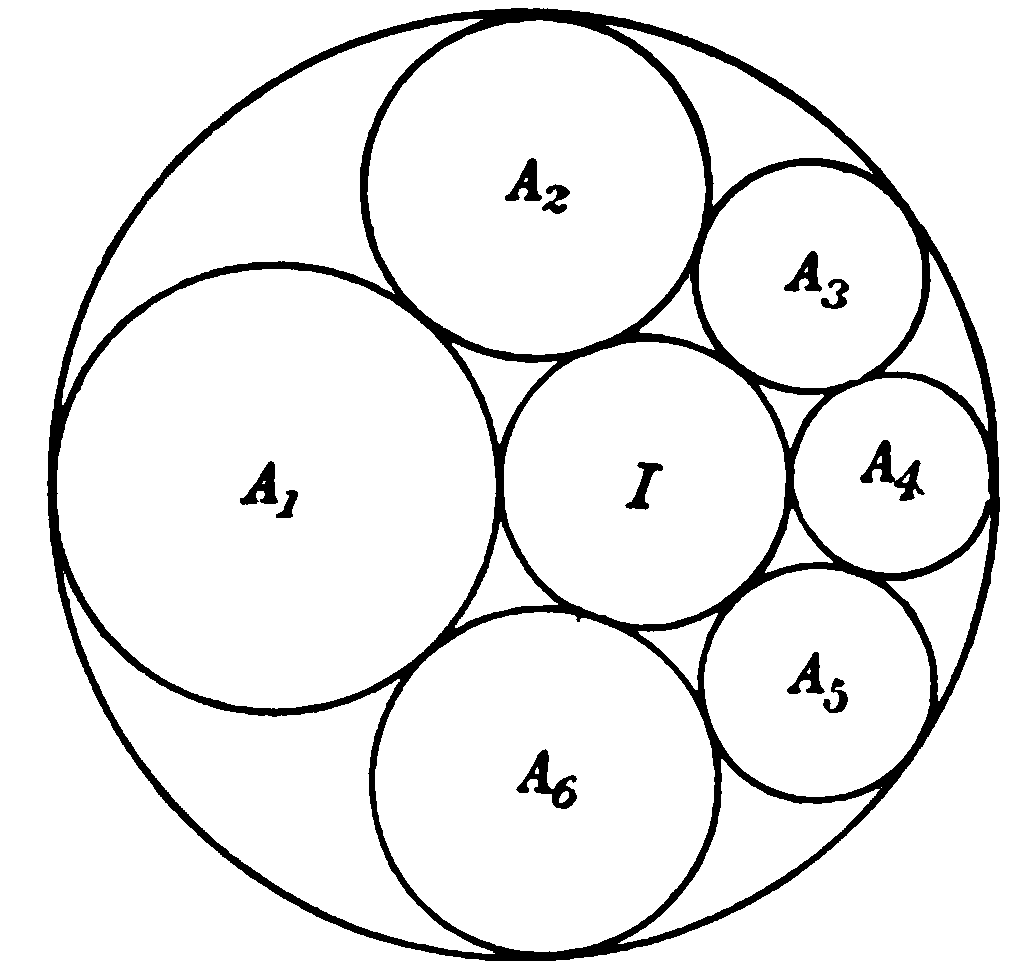
\includegraphics[width=0.42\linewidth]{pdf257-crown-inscribed-circles.png}
\end{center}

2. In the manuscript of 1784 Ajima first considers the case where the circle $A_1$ is described about the ``sagitta'' of the external
\scanfooter

\scanpage{0258}{Chapter 35, printed page 244}
and internal circles, or $E$ and $I$, which is the portion of the diameter common to both intercepted by their circumferences. In this case, writing
\[
\rho_2=A_1/A_2,\qquad \rho_3=A_1/A_3,\ldots
\]
and
\[
t=\frac{4EI}{(I+A_1)(E-A_1)},\qquad w=\rho_2-1,
\]
we shall have\footnote{These relations may be obtained in like way as in the last chapter. The derivation is, however, not explained in the manuscript before us.}
\[
\begin{aligned}
\rho_3&=tw+1,\\
\rho_4&=t^2w-2tw+\rho_2,\\
\rho_5&=t^3w-4t^2w+4tw+1,\\
\rho_6&=t^4w-6t^3w+11t^2w-6tw+\rho_2,\\
\rho_7&=t^5w-8t^4w+22t^3w-24t^2w+9tw+1,\ldots.
\end{aligned}
\]
Now if the number of the inscribed circles be 3, then $A_2$ and $A_3$ are to be equal, so that equating $\rho_2$ and $\rho_3$ we get
\[
tw+1-\rho_2=0,\qquad\text{or }tw-w=0,\qquad\text{or }t-1=0.
\]
When 4 circles are inscribed, $A_2$ is to be equal to $A_4$; and when 5 circles are inscribed, $A_3$ is to be equal to $A_4$; and thus equating the expressions for $\rho_2$ and $\rho_4$, $\rho_3$ and $\rho_4$, respectively, we obtain
\[
t-2=0\qquad\text{and}\qquad t^2-3t+1=0.
\]
Proceeding in this way we deduce the following equations:
\[
\begin{array}{rcl}
6\text{ circles:}&t^2-4t+3&=0,\\
7\text{ circles:}&t^3-5t^2+6t-1&=0,\\
8\text{ circles:}&t^3-6t^2+10t-4&=0,\\
9\text{ circles:}&t^4-7t^3+15t^2-10t+1&=0,\\
10\text{ circles:}&t^4-8t^3+21t^2-20t+5&=0,
\end{array}
\]
\[
\cdots\cdots\cdots\cdots\cdots\cdots\cdots\cdots
\]
It will be easy to see that the equations for even numbers of circles contain some superfluous factors---\emph{kwajo} in Japanese---which should be got rid of. Thus dividing the equations for the 6, 8, 10, \ldots circles by those for the 3, 4, 5, \ldots circles, respectively, then the equations for 4, 6, 8, \ldots circles will assume the forms:
\[
t-2=0,\qquad t-3=0,\qquad t^2-4t+2=0,
\]
\[
t^2-5t+5=0,\qquad t^3-6t^2+4t-2=0,\qquad t^3-7t^2+14t-2=0,\ldots.
\]
\scanfooter

\scanpage{0259}{Chapter 35, printed page 245}
In the equations of the circles of odd numbers there are also those that contain superfluous factors. If for instance we divide the equation for 9 circles with that for 3 circles we have
\[
t^3-6t^2+9t-1=0.
\]
In these equations we calculate the value of $t$. Then the relation
\[
(E-A_1)(I+A_1)t-4EI=0
\]
may be made use of in determining one of the quantities $E,I,A_1$ in terms of the other two.

Ajima then considers the case where there are described two equal circles $A_1$ touching along the sagitta as a common tangent.

3. The considerations in the ``Sequel'' of 1791 are intended in a more general way. From the same author's \emph{Renjutsu Henkan} of 1784, which we have mentioned in the last chapter, we have
\[
\begin{aligned}
&(I+E)^2A_1^2A_2^2-2m(E-I)A_1^2A_2-2m(E-I)A_1A_2^2\\
&\qquad{}+2m(E-I)A_1A_2s-2mnA_1A_2+m^2A_1^2+m^2A_2^2=0,
\end{aligned}
\]
where $s$ denotes the sagitta of $E$ and $I$ and
\[
m=IE+Es-Is-s^2,
\qquad n=EI+s^2.
\]
From this, by writing $t=4IE/m$, follows the equation for $A_2$:
\[
\begin{aligned}
&\{16I^2E^2+(I+E)^2A_1^2t^2-8(E-I)IEA_1t\}A_2^2\\
&\quad+\{32I^2E^2A_1-16I^2E^2A_1t-8(E-I)IEA_1^2t\}A_2+16I^2E^2A_1^2=0.
\end{aligned}
\]
Now proceeding as done in the \emph{Renjutsu Henkan} we get for $A_2$ the relation
\[
(-2+t+\rho-\varphi)A_2-2A_1=0,
\]
where
\[
\rho=\frac{2(E-I)A_1}{m},
\qquad
\varphi=\sqrt{4t-t^2+2(\rho+t)t-\frac{2\rho A_1t}{E-I}}.
\]
We thus get $\rho_2$, and consequently we get $A_2$. We have now to find the value of $t$, which is equal to $k+2$, the quantity $k$ being equal to $4IE/m-2$. We shall therefore first find $k$ for conveniency's sake. Thus
\[
\begin{aligned}
\rho_3&=\rho_2k+\rho-\rho_1=\rho_2k+(\rho-1),\\
\rho_4&=\rho_3k+\rho-\rho_2=\rho_2k^2+(\rho-1)k+(\rho-\rho_2),\\
\rho_5&=\rho_2k^3+(\rho-1)k^2+(\rho-2\rho_2)k+1,\\
\rho_6&=\rho_2k^4+(\rho-1)k^3+(\rho-3\rho_2)k^2-(\rho-2)k+\rho_2,\ldots.
\end{aligned}
\]
\scanfooter

\scanpage{0260}{Chapter 35 conclusion, printed page 246}
When there are inscribed 3 circles, the circles $A_1$ and $A_4$ as well as $A_2$ and $A_5$ should respectively coincide, so that equating $\rho_1$ and $\rho_4$ as well as $\rho_2$ and $\rho_5$, we have
\[
\alpha\equiv\rho_2k^2+(\rho-1)k+(\rho-\rho_2-1)=0,
\]
\[
\beta\equiv\rho_2k^3+(\rho-1)k^2+(\rho-2\rho_2)k+(1-\rho_2)=0,
\]
whence we get
\[
-\alpha k+\beta\equiv(-\rho_2+1)k+(1-\rho_2)=0,
\qquad\text{or}\qquad -k-1=0.
\]
In the case of four circles, the circles $A_1$ and $A_5$ as well as $A_2$ and $A_6$ respectively coincide, so that equating $\rho_1,\rho_5$ and $\rho_2,\rho_6$, we have, after the rejection of the factor $k$,
\[
\alpha\equiv\rho_2k^2+(\rho-1)k+(\rho-2\rho_2)=0,
\]
\[
\beta\equiv\rho_2k^3+(\rho-1)k^2+(\rho-3\rho_2)k-(\rho-2)=0,
\]
whence we have
\[
\gamma=\beta-\alpha k\equiv-\rho_2k-(\rho-2)=0,
\]
\[
\delta=\alpha+\gamma k\equiv k+(\rho-2\rho_2)=0,
\]
\[
\varepsilon=\gamma+\delta\equiv(-\rho_2+1)k-(2\rho_2-2)=0,
\qquad\text{or }-k-2=0.
\]
This value of $k$, however, does not agree with the data of the problem, so that here we have to take $k=0$.

In the same way the values of $k$ may be obtained for the cases of 5, 6, \ldots circles. Then using the relation $t=k+2$, we get the equations for 3, 4, 5, \ldots circles as follows:
\[
t-1=0,\qquad t-2=0,\qquad t^2-3t+1=0,
\]
\[
t-3=0,\qquad t^3-5t^2+6t-1=0,\qquad t^2-4t+2=0,\ldots.
\]
Now it will be seen that these equations are the same as those that give the ``moments''\footnote{Moments or modulus means the rates of quantities.} of the squares of the diagonals subtending two sides of the regular polygons having the same number of sides as there are inscribed circles in our case. We may therefore make use of the expressions for the diagonals instead of the values of $t$.

When the values of $t$ have been found, we have at once that of $\rho_2$ from the expression we have obtained in the above. And then $\rho_3,\rho_4,\ldots$ may be successively evaluated by virtue of the relation
\[
\rho_r=\rho_{r-1}k+\rho-\rho_{r-2}.
\]
\scanfooter

\scanpage{0261}{Chapter 36, printed page 247}
\begin{center}
CHAPTER 36.\\[1mm]
AIDA'S SOLUTION OF THE INDETERMINATE EQUATION\\
$x_1^2+x_2^2+x_3^2+x_4^2+x_5^2=y^2$.
\end{center}
\phantomsection\addcontentsline{toc}{subsection}{Chapter 36. Aida's Solution of the Indeterminate Equation $x_1^2+x_2^2+x_3^2+x_4^2+x_5^2=y^2$}

Problems in the indeterminate analysis were one of the favorite themes studied by the old Japanese mathematicians. One of the most striking instances among the numberless results obtained by them concerning this subject was certainly Aida Ammei's (1747--1817) solution of the equation
\[
x_1^2+x_2^2+x_3^2+x_4^2+x_5^2=y^2,
\]
as laid down in his manuscript \emph{Sampō Seisū-jutsu}.\footnote{The subjects described in this place follow the contents of C. Hitomi's article in the \emph{Journal of the Tokyo Physics School}, Vol. 15, pp. 359--362.} Aida's treatment may be applied at once to the case of any number of variables, so that we shall consider the problem in the generalised form
\[
x_1^2+x_2^2+x_3^2+\cdots+x_n^2=y^2.
\]
Aida's solution of this equation consists in
\[
x_1=-a_1^2+a_2^2+a_3^2+\cdots+a_n^2,
\]
\[
x_r=2a_1a_r\qquad(r=2,3,\ldots,n),
\]
where $a_1,a_2,a_3,\ldots,a_n$ are any integers. The legitimacy of this solution may be easily verified thus: The left side is
\[
=a_1^4-2a_1^2\sum a_r^2+(\sum a_r^2)^2+4a_1^2(\sum a_r^2)
=(a_1^2+a_2^2+\cdots+a_n^2)^2,
\]
which proves that $y$ is also of the integral form. Here we have written the symbol $\sum$ to designate a sum extending for the values of $r$ from 2 to $n$. This designation will be followed throughout in this chapter.

If for instance we take $n=5$ the following numerical values will be obtained:
\begin{center}
\small
\begin{tabular}{|r|r|r|r|r||r|r|r|r|r|r|}
\hline
$a_1$&$a_2$&$a_3$&$a_4$&$a_5$&$x_1$&$x_2$&$x_3$&$x_4$&$x_5$&$y$\\
\hline
5&4&3&2&1&5&40&30&20&10&55\\
4&3&2&1&5&23&24&16&8&40&55\\
3&2&1&5&4&37&12&6&30&24&55\\
2&1&5&4&3&47&4&20&16&12&55\\
1&5&4&3&2&53&10&8&6&4&55\\
\hline
\end{tabular}
\end{center}
\scanfooter

\scanpage{0262}{Chapter 36 conclusion, printed page 248}
Next Aida gives rules of solution for various other equations allied in form to the one just considered. Some of these are reproduced in generalised forms in the following lines:

Equation:
\[
1x_1^2+2x_2^2+3x_3^2+\cdots+nx_n^2=y^2
\]
has the solution (for $r=2,3,\ldots,n$)
\[
x_1=-a_1^2+\sum ra_r^2,
\qquad x_r=2a_1a_r,
\]
for the left-hand side of the equation is
\[
=a_1^4-2a_1^2\sum ra_r^2+(\sum ra_r^2)^2+\sum r(4a_1^2a_r^2)
=(a_1^2+2a_2^2+3a_3^2+\cdots+na_n^2)^2.
\]
In the equation
\[
x_1^2+3x_2^2+6x_3^2+\cdots+\frac{n(n+1)}2x_n^2=y^2,
\]
Aida takes the solution
\[
x_1=-a_1^2+3a_2^2+6a_3^2+10a_4^2+\cdots+\frac{n(n+1)}2a_n^2,
\]
\[
x_r=2a_1a_r\qquad(r=2,3,\ldots,n).
\]
For here we have
\[
\begin{aligned}
a_1^4-2a_1^2\sum\frac{r(r+1)}2a_r^2
+\left(\sum\frac{r(r+1)}2a_r^2\right)^2
+\sum\frac{r(r+1)}2(4a_1^2a_r^2)\\
=\left\{a_1^2+3a_2^2+6a_3^2+10a_4^2+\cdots+\frac{n(n+1)}2a_n^2\right\}^2.
\end{aligned}
\]
If in general $p_1,p_2,p_3,\ldots$ be the figurative numbers of any order or polygonal numbers, still the way of solution applies to the equation
\[
p_1x_1^2+p_2x_2^2+p_3x_3^2+\cdots+p_nx_n^2=y^2,
\]
as C. Hitomi mentions in his article.\footnote{After the above article was written I have seen Aida's original work, in which it appears that the author has intended to show his solution applicable to the general case not restricted to the sum of five squares. He has also solved equations of the forms
\[
1x_1^2+4x_2^2+9x_3^2+\cdots=y^2,
\]
and
\[
1x_1^2+9x_2^2+36x_3^2+100x_4^2+\cdots=y^2.
\]
The solutions of these equations are all of the same forms as we have given in the text. The composition of Aida's work was not anterior to 1807, as a passage in it concerns a work of Sakabe Kōhan that bears this date. It appears Ajima Chokuyen had anticipated Aida in some points about what we have mentioned in this chapter.}
\scanfooter

\scanpage{0263}{Chapter 37 opening, printed page 249}
\begin{center}
CHAPTER 37.\\[1mm]
AIDA'S STUDIES ON THE ELLIPSE.
\end{center}
\phantomsection\addcontentsline{toc}{subsection}{Chapter 37. Aida's Studies on the Ellipse}

1. Aida Ammei wrote the manuscript \emph{Sampō Sokuyen Shū} consisting of twenty books, in which he laid down the results of his considerations about the ellipse and allied subjects. Although the date of his composition is not known, yet certainly it was the production of his old age. In subsequent ages the properties of the ellipse became one of the favourite subjects of the Japanese mathematicians, but so far as we know Aida was the first scholar who carried on extensive studies on the ellipse in earlier days.

2. The most striking point in Aida's work is perhaps the employment of an instrument called \emph{sokuyen-ki} or ``ellipse-describer''. This is a contrivance by which the two foci of an ellipse are fastened by a string of pre-determined length. The use of the focal property in describing an ellipse would appear no extraordinary event to those who are accustomed to consider the curve in reference to its foci. But when we reflect that the focal properties were not taken into account by the Japanese mathematicians in general, we cannot help being interested to find such an instrument used by Aida. In book 6 Aida describes of it as follows:

``If one desires to describe an ellipse, he should first construct an ellipse-describer, without the aid of which the actual form of the curve can hardly be obtained. The instrument is made of a flat wooden board, on which two needles are provided. The first of these needles is fixed, while the second is so adjusted that it may be slided freely along the gutter cut through the board, thus making it possible to take any lengths for the major and minor diameters. Besides, a jointer must be used, on which a string-stop should be provided at the board's thickness from its end, and a \emph{fude} or `wool-pencil'\footnote{With which the Japanese used to write. There was no pencil in Japan.} is to be jointed to the jointer on describing the curve. If thus, for instance, an ellipse is to be described with the major diameter 5 units and the minor diameter 3 units, we have to take a string 9 units long, making the distance between the two needles 4

\begin{center}
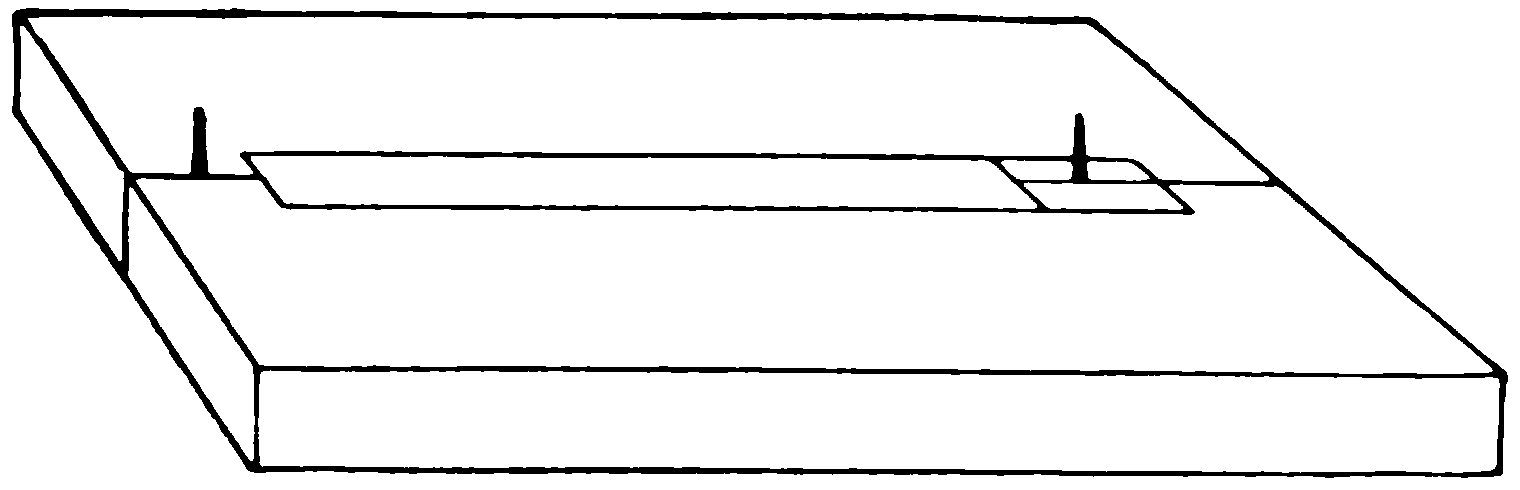
\includegraphics[width=0.62\linewidth]{pdf263-ellipse-describer.png}
\end{center}
\scanfooter

\scanpage{0264}{Chapter 37, printed page 250}
units. If we now stretch the string tightly, the wool-pencil will take a position $0\dd5$ units in front of the first needle, the form of the string now consisting of two partly coincident lines. This is the point whence the curve will begin to be described. If we then turn the wool-pencil as it would go naturally with the string stretched, the string forms always the two sides of a triangle. When it reaches the minor diameter, the triangle becomes isosceles. Described in this way, never making the string loose, we get the natural form of the ellipse.''

Aida does not make any mention as to whence he had learned of the instrument. But his pupil Ichino Mokyō writes in his manuscript, \emph{Dayen-shū Tsūjutsu} of 1820, that an instrument for describing the ellipse was brought from abroad, together with some theories concerning the curve. The ellipse-describer we have just described must have been the instrument referred to by Ichino though we know nothing definitely.\footnote{The ellipse-describer constructed by Hazama Jufū is more interesting than that of Aida and something will be mentioned of it in another place. I have learned of the instrument after the composition of the present work.}

3. Here we shall see something of what Aida studies of the focal properties of the ellipse, because a similar way of consideration is hardly to be met with among the writings of his contemporaries or among those of after-ages.

Let $a,b,c,k$ be the major diameter, minor diameter, focal distance and length of the string,\footnote{Of course the two ends of the string are both fastened to one of the needles and go around the other.} respectively. Then $a-c$ is twice the length between one of the needles and the end of the major diameter. If we add $2c$ thereto, we obtain $k=a+c$. We have also
\[
\left(\frac{k-c}{2}\right)^2-\left\{\left(\frac c2\right)^2+\left(\frac b2\right)^2\right\}=0
\qquad\text{or}\qquad a^2-b^2-c^3=0,
\]
which serves for the determination of $c$ in terms of $a$ and $b$. In the figure let the sagitta $AD=s$ be given, and let the chord $PP'=h$ be required. Here we have
\[
PF_2^2=(a-PF_1)^2=(F_1D+F_1F_2)^2+PD^2,
\]
whence follows
\[
a^2-2a\dd PF_1-ac+2sc=0,
\qquad\text{or}\qquad (a^2-ac+2sc)^2-(2a\dd PF_1)^2=0,
\]

\begin{center}
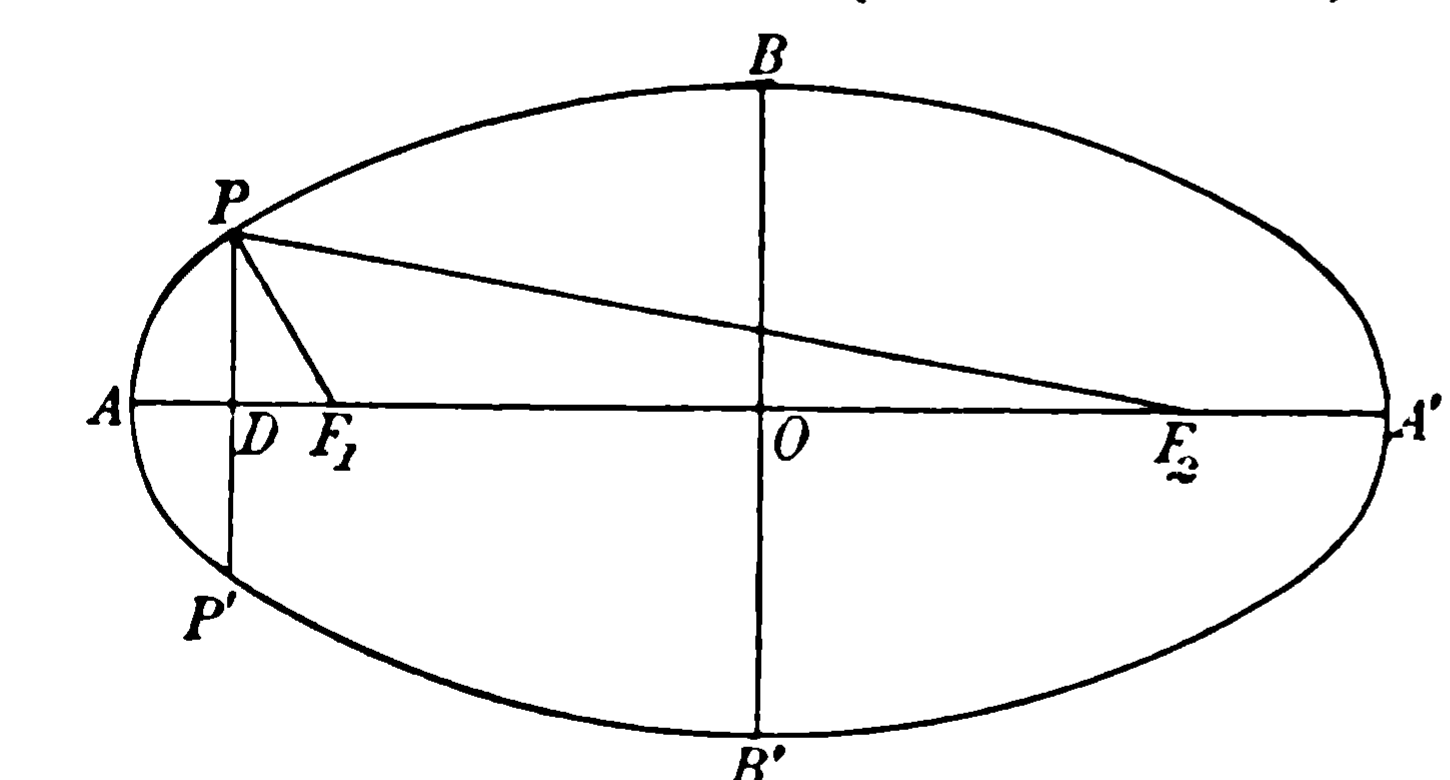
\includegraphics[width=0.55\linewidth]{pdf264-ellipse-focal-chord.png}
\end{center}
\scanfooter

\scanpage{0265}{Chapter 37, printed page 251}
but
\[
PF_1^2=PD^2+F_1D^2=PD^2+\left(\frac a2-\frac c2-s\right)^2,
\]
\[
\therefore\quad b^2as-b^2s^2-a^2PD^2=0,
\qquad\text{or}\qquad h=2\dd PD=2\sqrt{\frac{asb^2-s^2b^2}{a^2}}.
\]
Thus it will be seen that the elliptic chord $h$ is obtained from the corresponding chord of the circle with $a$ as diameter by multiplying by $b/a$. It follows theréfere that the areas of an elliptic segment or of an entire ellipse may be obtained from the corresponding areas of a circle by multiplying by $b/a$. About this point Aida further tries a mode of demonstration. For, let $c_r$ be the chords parallel to the minor diameter at equal intervals, $l$ say. Then $c_r$ will be expressed by $\frac ba\times c'_r$, where $c'_r$ are the corresponding chord of the circle about $a$ as diameter. But the area of the circular segment is
\[
\lim_{l=0}\sum\left\{\frac12(c'_r+c'_{r+1})l\right\},
\]
while that of the elliptic segment is
\[
\begin{aligned}
\lim_{l=0}\sum\frac{c_r+c_{r+1}}2\times l
&=\lim\sum\frac12\left(c'_r\frac ba+c'_{r+1}\frac ba\right)\times l\\
&=\frac ba\lim\sum\left(\frac{c'_r+c'_{r+1}}2\right)\times l,
\end{aligned}
\]
or $b/a$ times of the circular segment. It is also evidently the same for the whole area of the ellipse.

4. In the case of a segment which is cut obliquely through the end of the minor diameter, let $c$ be the chord of the segment, and let $h$ and $k$ be the ordinate and abscissa of the end-point of the chord $c$, the corresponding ordinate of the circle about the major diameter being $h'$. Here these lengths are assigned to terminate at the major and minor diameters. The relation that exists between the length and breadth of a rectangle inscribed in an ellipse will be found to be
\[
a^2b^2-(\text{length})^2b^2-(\text{breadth})^2a^2=0,
\]
so that writing the two sides of the rectangle $2h$ and $2k$ respectively and having reference to the expression
\[
k^2=c^2-\left(\frac bc-h\right)^2,
\]
we have
\[
a^2b^2-4c^2b^2+4h^2b^2-4hb^3+b^4-4a^2h^2=0,
\]
from which $h$ can be determined in terms of $a,b$, and $c$.
\scanfooter

\scanpage{0266}{Chapter 37, printed page 252}
Again we have
\[
h'=h\times\frac ab\qquad\text{and}\qquad c'^2=k^2+\left(\frac12a-h'\right)^2,
\]
where $c'$ is the circular chord corresponding to $c$. Thus the area of the circular segment with the chord $c'$ may be found, and Aida draws the conclusion without further considerations that the elliptic segment is $b/a$ times of the circular segment.

The same result will be obtained if the segmental chord be drawn from an end of the major diameter.

5. Aida's rectification of the ellipse is of some interest, for it is effected according to a principle different from those that were employed by other Japanese mathematicians. In the first place Aida maintains that the segmental area bounded by the chord joining the ends of the major and minor diameters may be taken for the first approximation to the length of a quadrantal arc. If we draw an ordinate at the middle of half the major diameter the sum of the two segmental areas bounded by the two arcs thus divided and their respective chords will afford the second approximation. Next divide the half major diameter into four equal parts drawing the ordinates at the points of division. The areas of the four segments bounded by the four arcs divided by these ordinates and their respective chords being added together, their sum is to be taken for the third approximation. Proceeding in this way successive approximations will be obtained. When we come thus to the number of divisions which may be counted by tens of thousands, the segmental area will become so exceedingly thin that it can be practically considered as representing the length of the arc of the segment. Thus we ultimately arrive at the value of the length of the arc of the quadrant.

Aida expressly argues in this way, but he does not seem to follow exactly this rule in actual calculations. For he says further that the expressions for the successive chords in the ellipse being found, these will be seen not to be proportional to the cerresponding lengths in the circle described about the major diameter. The elliptic perimeter, therefore, he concludes, cannot be found as proportional to the circular circumference. Consequently he makes the calculation as follows. Writing $t=a/2n$, the ordinates of the auxiliarly circle at the points of division and terminated at the major diameter will be
\[
p_1'^2=(a-t)t,
\qquad p_2'^2=(a-2t)2t,
\qquad p_3'^2=(a-3t)3t,\ldots;
\]
\scanfooter

\scanpage{0267}{Chapter 37, printed page 253}
whence writing $m=b/a$ we obtain the corresponding ordinates for the ellipse, $p_1=p'_1m$, $p_2=p'_2m$, $p_3=p'_3m,\ldots$, and the successive chords of the elliptic arcs are found to be
\[
c_1^2=t^2+p_1^2,
\qquad c_2^2=t^2+(p_2-p_1)^2,
\qquad c_3^2=t^2+(p_3-p_2)^2,\ldots.
\]
Aida goes no further than this in his consideration. He was not perhaps possessed of the final formula expressing the value of the elliptic perimeter in a convenient form, a perfection which was left to the hands of his successors to complete. About the studies of the same subject by the mathematicians Sakabe, Kawai, Ichino, Tani, Shiraishi, Wada, etc., we hope we shall one day be able to give a detailed account.

6. In Book 20 of his work Aida considers obtaining a relation that exists when four equal circles are described touching an ellipse externally so that their centres form a rectangle. For this purpose he describes two figures as annexed. In the first figure the circle $B$ is described touching two of the four equal circles. From $C$, the point of contact, $CK$ is let fall perpendicular to the major diameter. Here we shall denote the major and minor diameters by $a$ and $b$, the sides of the rectangle by $h$ and $k$, of which we take the former to be parallel to $b$, and the diameters of the circles $A$ and $B$ by these letters. Let $M$ be the point of intersection of $h$ and $a$. In the second of the figures a rectangle is represented, of which the diagonal is equal to $a$ and one side $=b$. Let $O'$ be the centre, and take $O'B'$ on the diagonal equal to $OB$. Draw $B'P$ at right angles to it, ending in the line through $O'$ parallel to a side; draw $PK'$ parallel to another side. It is noted that $K'$ is the point where the circles $A$ and $B$ touch the ellipse.

\begin{center}
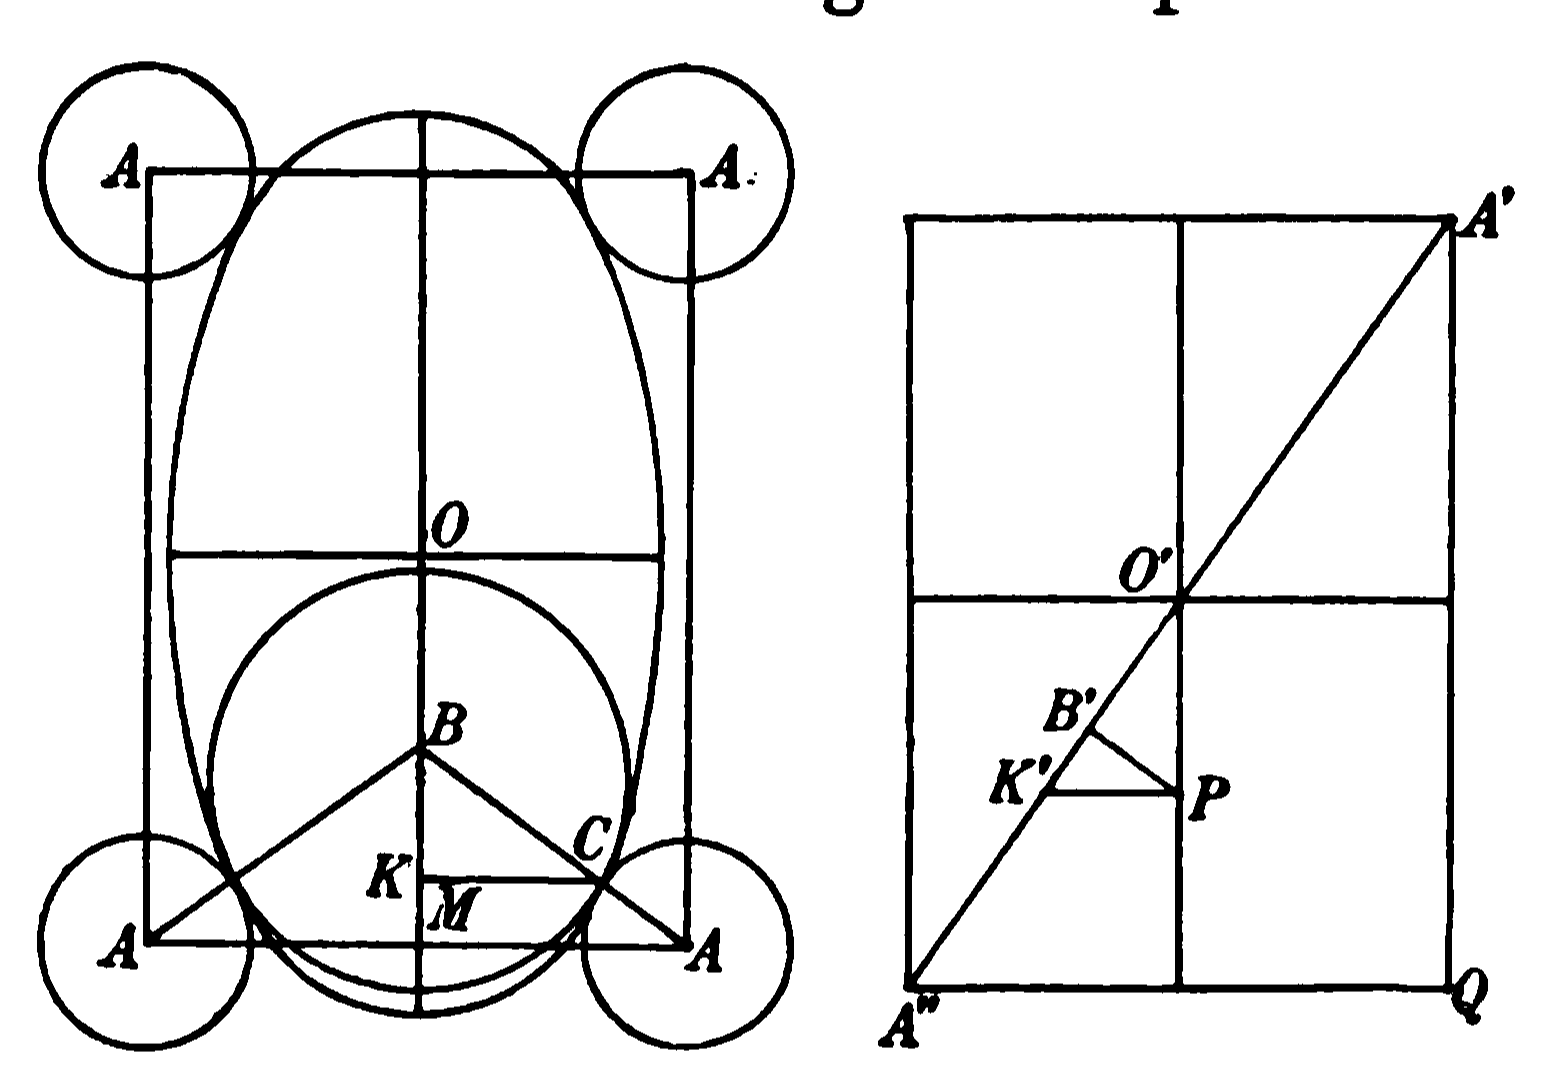
\includegraphics[width=0.76\linewidth]{pdf267-external-circles-projection-pair.png}
\end{center}

Now without explanation the author gives these relations:
\[
\alpha^2=A'Q^2=a^2-b^2,
\qquad \beta^2=B'P^2=\frac{b^2-B^2}{4},
\qquad \gamma=OB=O'B'=\frac{\beta\alpha}{4},
\]
\[
\delta=BK=B'K'=\frac{\beta b}{\alpha},
\qquad \varepsilon=BM=\frac k2-\gamma.
\]
We have then
\[
\frac B2:\frac{A+B}{2}=\delta:\varepsilon,
\qquad\text{or}\qquad \gamma B+\delta(A+B)=\frac{Bk}{2},
\]
\scanfooter

\scanpage{0268}{Chapter 37, printed page 254}
which, on squaring and rewriting, gives
\[
\beta^2\alpha^4B^2+2\beta^2\alpha^2b^2(A+B)B+\beta^2b^4(A+B)^2-\frac14k^2B^2\alpha^2b^2=0,
\]
or
\[
\tag{1}(\alpha^2B+b^2A^2)\beta^2-\frac14k^2B^2\alpha^2b^2=0.
\]
Again writing $\xi^2=CK^2=\frac14B^2-\delta^2$, we have
\[
\xi:\frac h2=\frac B2:\frac{A+B}{2},
\qquad\text{or}\qquad \xi^2(A+B)^2-\frac14B^2h^2=0,
\]
whence we get
\[
\tag{2}(A+B)^2a^2B^2-(A+B)^2b^4-h^2\alpha^2B^2=0.
\]
From the relations (1) and (2) follows
\[
\begin{aligned}
b^6A^2+(2b^4a^2A)B+(b^2a^4-b^4A^2-k^2b^2\alpha^2)B^2\\
{}-(2b^2a^2A)B^3-a^4B^4=0,
\end{aligned}
\]
\[
-b^4A^2-(2b^4A)B-(b^4-a^2A^2+h^2\alpha^2)B^2+(2a^2A)B^3+a^2B^4=0,
\]
whence the elimination of $B$ gives the required relation in the form
\[
P^2Q^2+4Q^3a^2b^2A^2+4P^3+18PQa^2b^2A^2-27a^4b^4A^4=0,
\]
where $P$ and $Q$ are written for
\[
-a^2A^2-b^2A^2-a^2b^2+h^2a^2+k^2b^2,
\qquad -a^2-b^2-A^2+h^2+k^2.
\]
7. This same problem is considered in still another way, which is very interesting, as a kind of projection is resorted to, although I am little able to fully understand the construction used. To quote the auther's own words in a translation as literal as the case will admit, ``This problem may be considered, as will seem from the figure annexed\footnote{Here we omit the figure.}, as arising from a circular cylinder, which is touched by spheres, by cutting with a plane through the points where the spheres touch the elliptic perimeter of the section, whereby the circles $A$ will be produced in the section plane touching the ellipse. We may therefore consider the five quantities presented in the data of the problem together with an additional one, constituting six in all, and form two expressions for the diameter of the sphere, when we have to effect the cross multiplications\footnote{Here Aida uses the same word \emph{shajō} or cross multiplications, which Seki Kōwa used in his treatment of the determinant. Aida has perhaps applied the same theory as done by Seki, though the details of calculations are not indicated.} of these expressions and thus arrive at the required relation.''
\scanfooter

\scanpage{0269}{Chapter 37, printed page 255}
For the purpose of constructing the two expressions just mentioned, a figure is drawn such as shown here. The diameter of the sphere being $S$, we write
\[
\alpha^2=a^2-b^2,
\qquad \beta^2=\frac{S^2-A^2}{4},
\qquad \gamma=\frac{\beta a}{\alpha},
\]
\[
\delta^2=\frac{S^2}{4}-\gamma^2,
\qquad \varepsilon=\frac{\beta b}{\alpha},
\qquad \zeta=\frac k2-\varepsilon,
\qquad \Phi=\frac{\zeta b}{a},
\]
and we have
\[
\frac h2:\delta=\frac{S+b}{2}:\frac S2,
\]
or
\[
(S+b)^2\delta^2-\frac{S^2h^2}{4}=0,
\]
or (1)
\[
(S+b)^2S^2\alpha^2-(S+b)^2S^2a^2+(S+b)^2A^2a^2-h^2S^2\alpha^2=0.
\]
Again we have
\[
\Phi:\gamma=\frac b2:\frac S2,
\qquad\text{or}\qquad \Phi S-\gamma b=0,
\]
whence we get
\[
\tag{2}\frac{k^2S^2\alpha^2}{4}-\beta^2(bS+a^2)^2=0.
\]

\begin{center}
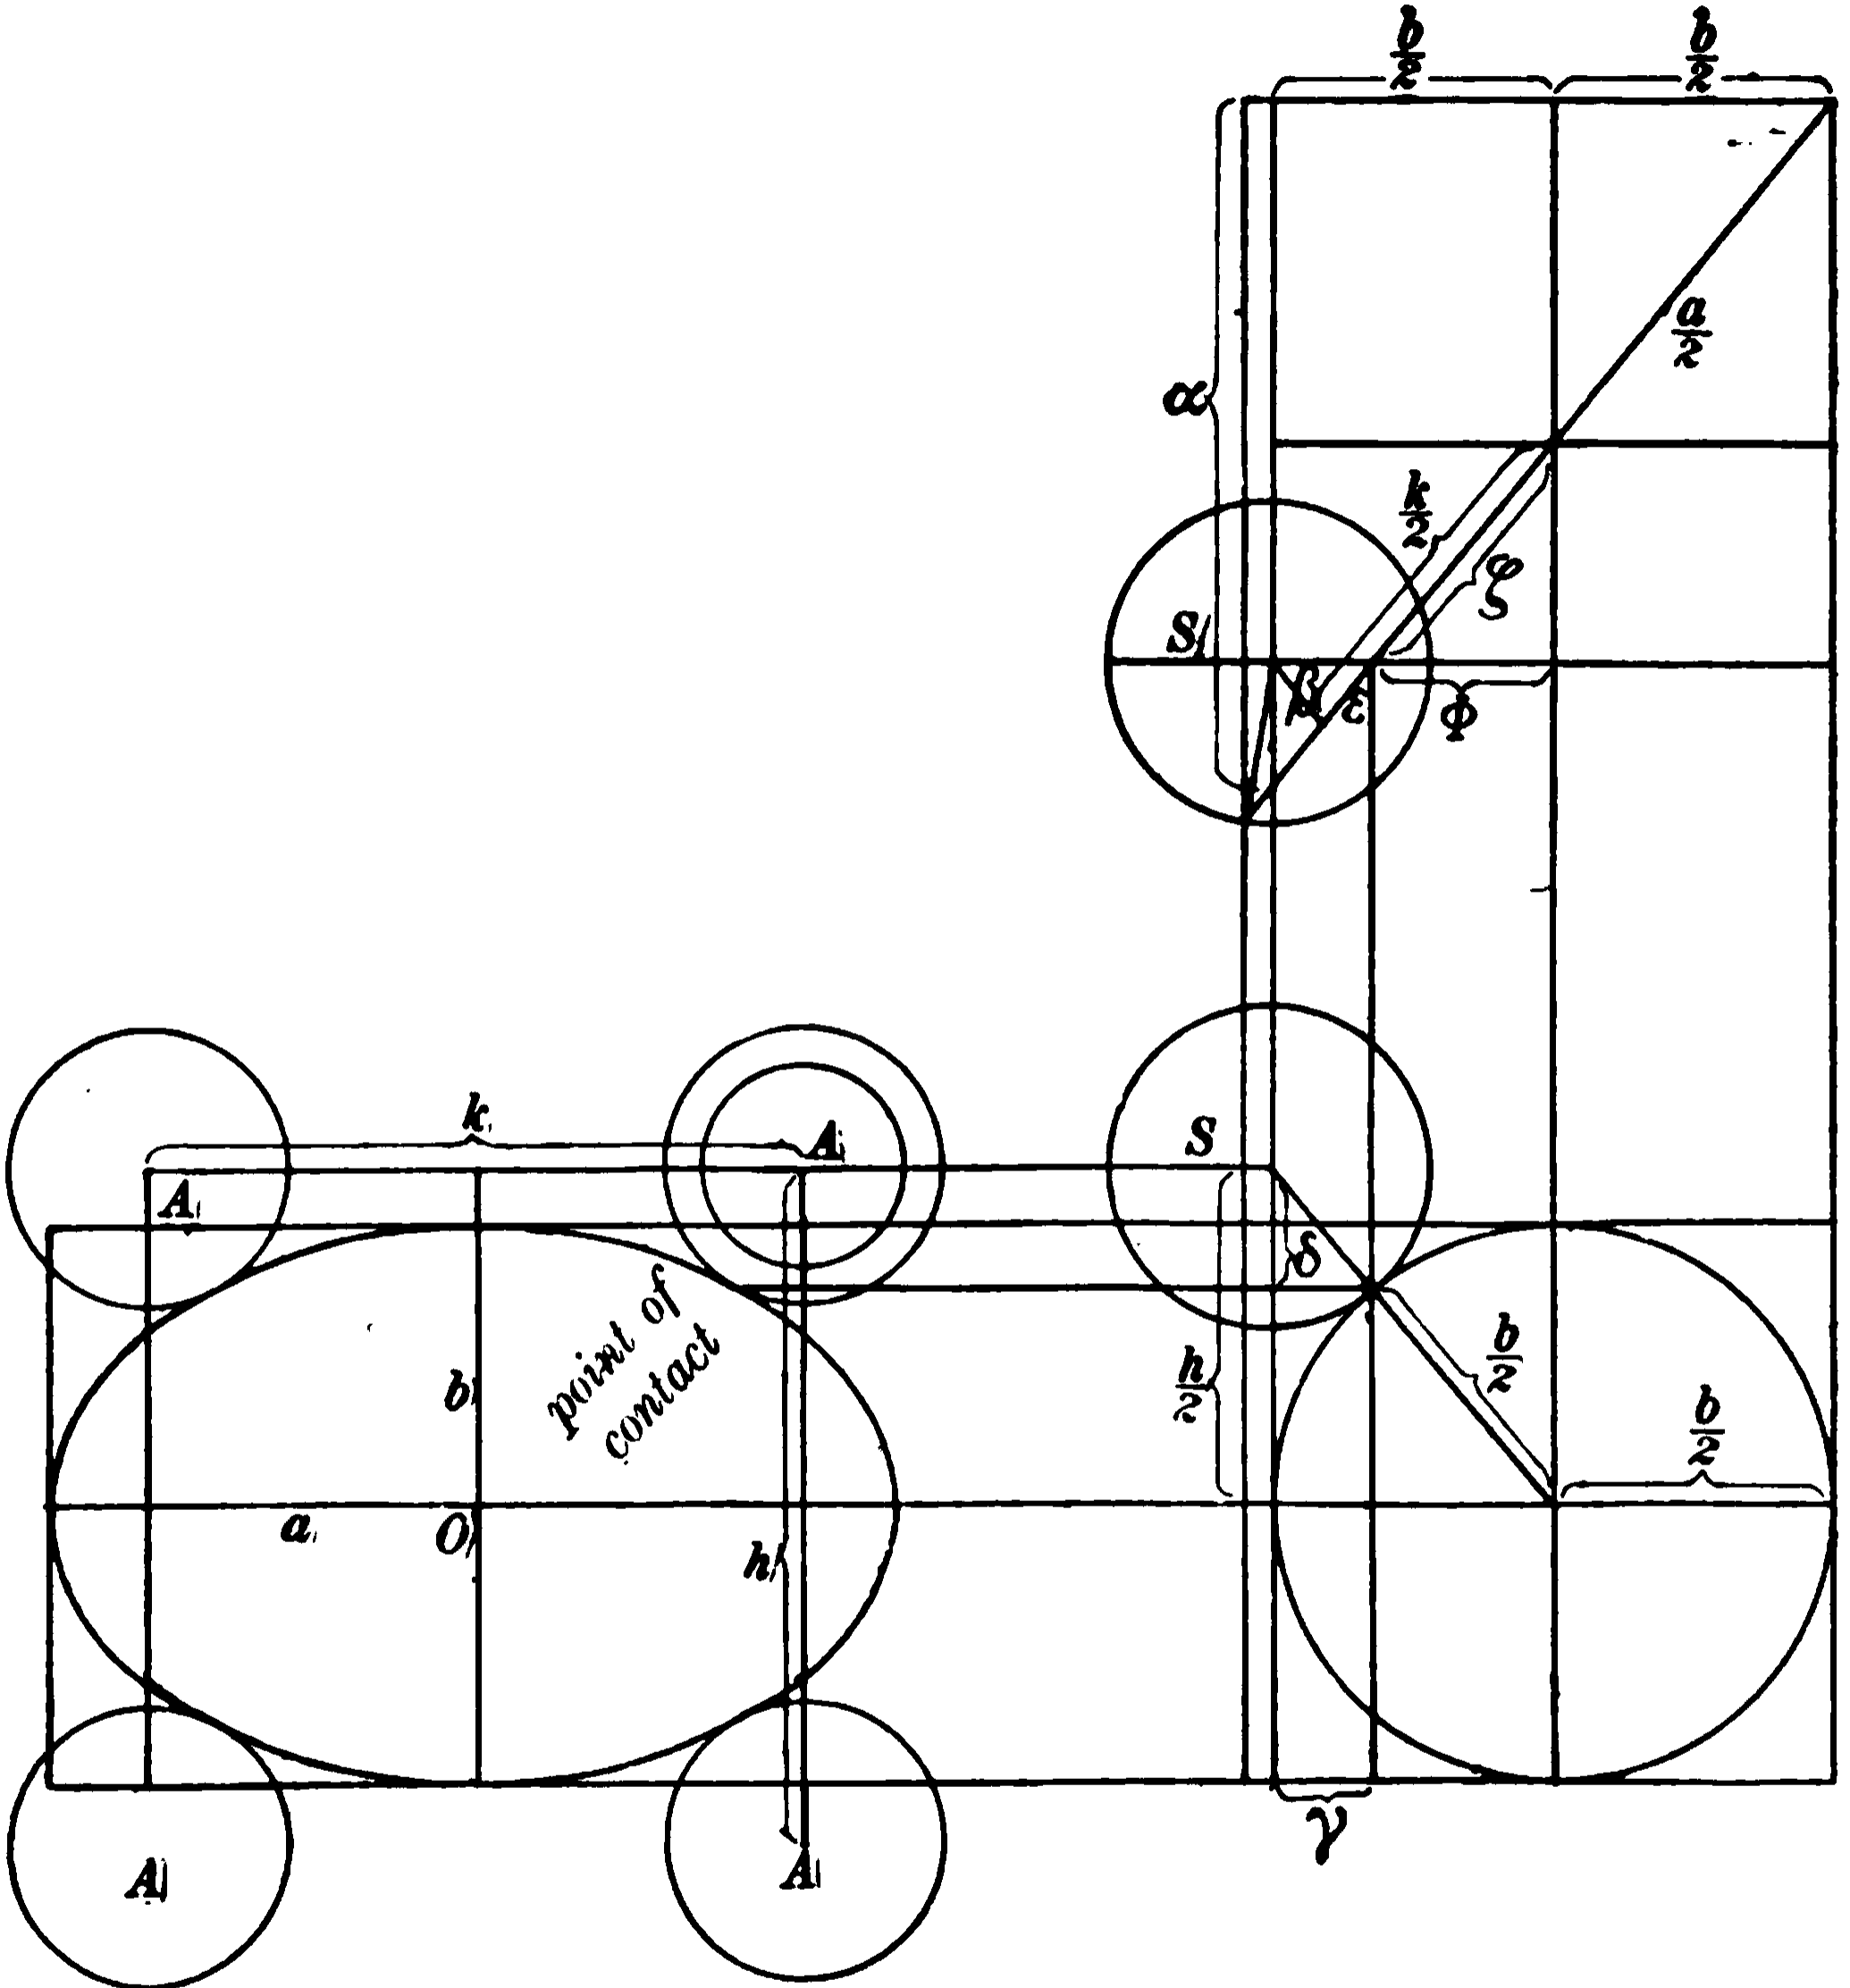
\includegraphics[width=0.82\linewidth]{pdf269-sphere-cylinder-projection.png}
\end{center}

From these two relations we have
\[
b^2a^2A^2+(2a^2A^2b)S+(a^2A^2-b^4-h^2\alpha^2)S^2-(2b^3)S^3-b^2S^4=0,
\]
\[
A^2a^4+(2A^2ba^2)S+(A^2b^2-a^4+k^2\alpha^2)S^2-(2a^2b)S^3-b^2S^4=0.
\]
Here eliminating $S$ by cross multiplication we obtain the same relation as arrived at previously.

Thus the author adds that in the two ways of procedure, we have tried, the same formula has been deduced, which shows the legitimacy of the result obtained.

8. Aida further considers the problem of finding the radii vectores of an ellipse drawn from the centre for every minute of angle. To solve this problem the chords drawn through the ends of the radii vectores parallel to the major and minor diameters are to
\scanfooter


\scanpage{0270}{printed page 256}
be found. Let these be denoted by $c_r$ and $p_r$. Then the required lengths will be found to be expressed by the formula:
\[
-a^2b^2+(a^2c_r^2+b^2p_r^2)\,\varrho_r=0.
\]

Though there are various other points in the manuscript that are worthy of remark, we shall not enter into detailed discussion of them in this place, because we fear lest it should drive us into tediousness.

\begin{center}
CHAPTER 38.\\[1mm]
SHIRAISHI'S CALCULATION OF THE ELLIPSOIDAL SURFACE.
\end{center}
\phantomsection\addcontentsline{toc}{subsection}{Chapter 38. Shiraishi's Calculation of the Ellipsoidal Surface}

Studies of the ellipsoid of revolution were not rare among the writings of the old Japanese mathematiciaus, but it is not so common for us to meet with results of their studies of the ellipsoid. We have however some documents concerning the subject, and a remarkable instance is furnished in a problem in Shiraishi Chōchū's \emph{Shamei Sampu}, Book II., published in 1826. The problem relates to the evaluation of the surface of an ellipsoid. In this book the result only is given, the analysis being not described. Let $a$, $b$, $c$ be the three principal diameters, and form the quantities:
\[
S=\left(1-\frac{c^2}{a^2}\right)\left(1-\frac{c^2}{b^2}\right),\quad N=1-\frac{1}{2}\left(\frac{c^2}{a^2}+\frac{c^2}{b^2}\right).
\]
Then $ab\pi$ is called the original term, which we denote by $D_0$; $\frac{1}{1\cdot 3}D_0N$ is the first difference $D_1$. The second, third, \dots\ differences $D_2, D_3, \dots$ will be formed in this way:
\begin{gather*}
D_2=\frac{1\cdot 3}{2\cdot 5}\left\{D_1N-\frac{1}{3^2}D_0S\right\},\quad D_3=\frac{3\cdot 5}{3\cdot 7}\left\{D_2N-\frac{1\cdot 2}{5^2}D_1S\right\},\\
D_4=\frac{5\cdot 7}{4\cdot 9}\left\{D_3N-\frac{3\cdot 3}{7^2}D_2S\right\},\quad D_5=\frac{7\cdot 9}{5\cdot 11}\left\{D_4N-\frac{5\cdot 4}{9^2}D_3S\right\},\dots,
\end{gather*}
and the original term $D_0$ being diminished by the successive differences gives the formula for the surface of the ellipsoid.

This formula is given in the \emph{Shamei Sampu} in the name of the author's pupil Ikeda Tei-ichi, whose authorship seems however to be only nominal, for there remains a manuscript written by his master, dated the 13\textsuperscript{th} day of the 6\textsuperscript{th} month of 1824. In old Japan the master's results were sometimes published in his pupils' names. Various publications abound actually with a great number of such instances.

\scanpage{0271}{printed page 257}
In the following lines we have to describe Shiraishi's treatment of the problem.\footnote{The expressions given in the text may not be very correct owing to various causes, but our account will be enough to show the essence of the process followed by the author.}

For the purpose of finding the surface of an ellipsoid Shiraishi constructs a figure as shown here.
\begin{center}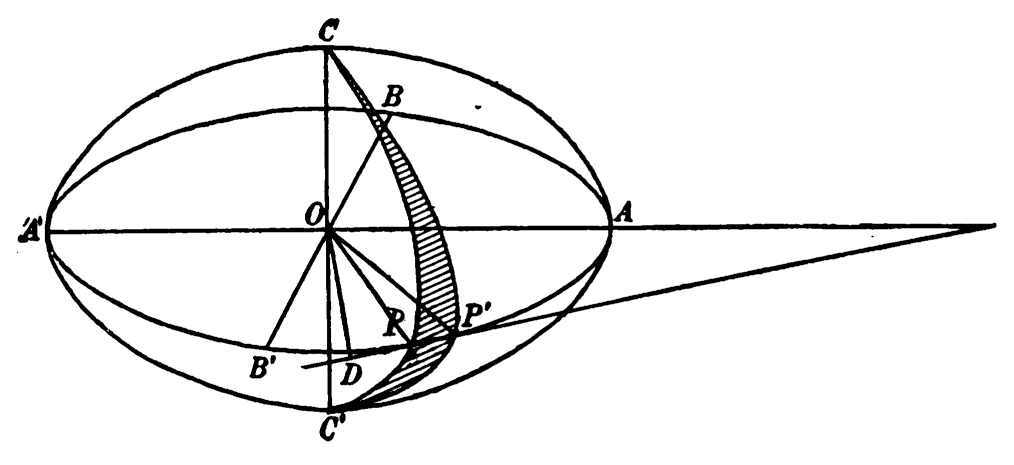
\includegraphics[width=0.6\linewidth]{pdf271-a.png}\end{center}
Suppose $AA'=a$ is divided into $2n$ equal parts by planes normal to it. Let two successive planes of the series meet the section of the ellipsoid made by the plane of $AA'=a$ and $BB'=b$ in the points $P$ and $P'$. Then we take $2.PP'=s_r$ for the element of arc of that section, and have
\[
s_r^2=\frac{1}{l}\left\{k^2-\frac{Bk^4r^2}{a^2}\right\},
\]
where
\[
k=\frac{a}{n},\quad l=1-\frac{k^2r^2}{a^2},\quad B=1-\frac{b^2}{a^2}.
\]
If $p_r$ denotes the perpendicular $OD$ dropped from the contre $O$ upon the line of $PP'$, we have $p_r=kb/s_r\sqrt{l}$.

These relations are given without explanation, being stated as explained in a different manuscript, but we shall not concern ourselves here about these matters.

Now Shiraishi considers the strip of the ellipsoidal surface cut off by two planes through the axis $CC'=c$ and through the points $P$ and $P'$ respectively. Such a strip is indicated in the figure by the ruled portion, which is taken as the element of area or $S_r$, and Shiraishi gives the following formula
\[
S_r=2s_rp_r\left(1-\frac{C}{1\cdot3}-\frac{C^2}{3\cdot5}-\frac{C^3}{5\cdot7}-\frac{C^4}{7\cdot9}-\cdots\right),
\]
where $C$ is written in place of $1-\frac{c^2{s_r}^2l}{b^2k^2}$. Shiraishi does not explain the construction of this formula in the manuscript before us but he only indicates by way of a figure that it has been obtained from assuming the element of area to be given by a corresponding portion

\scanpage{0272}{printed page 258}
\noindent of an elliptic cylinder, whose base is an ellipse with $c$ and $2p_r$ as the principal diameters, which is cut by two planes drawn through the diameter $c$, cutting the length $s_r$ from the generating line at the middle part of it.

Writing $A=1-c^2/b^2$, the quantity $C$ may be written
\[
C=1-\frac{c^2s_r{}^2l}{k^2b^2}=A+\frac{Bc^2k^2r^2}{a^2b^2}.
\]

Thus the expression for $S_r$ becomes
\[
\begin{array}{r@{}l@{}l@{}l@{}l@{}l@{}l}
=\dfrac{b}{\sqrt{l}}\Biggl\{\qquad k\biggl( & 1 & {}-\dfrac{A}{1\cdot 3} & {}-\dfrac{A^2}{3\cdot 5} & {}-\dfrac{A^3}{5\cdot 7} & {}-\dfrac{A^4}{7\cdot 9} & {}-\cdots\biggr)\\[2mm]
{}+\dfrac{Bc^2k^3r^2}{b^2a^2}\biggl( & & {}-\dfrac{1}{1\cdot 3} & {}-\dfrac{2A}{3\cdot 5} & {}-\dfrac{3A^2}{5\cdot 7} & {}-\dfrac{4A^3}{7\cdot 9} & {}-\cdots\biggr)\\[2mm]
{}+\dfrac{B^2c^4k^5r^4}{b^4a^4}\biggl( & & & {}-\dfrac{1}{3\cdot 5} & {}-\dfrac{3A}{5\cdot 7} & {}-\dfrac{6A^2}{7\cdot 9} & {}-\cdots\biggr)\\[2mm]
{}+\dfrac{B^3c^6k^7r^6}{b^6a^6}\biggl( & & & & {}-\dfrac{1}{5\cdot 7} & {}-\dfrac{4A}{7\cdot 9} & {}-\cdots\biggr)\\[2mm]
{}+\dfrac{B^4c^8k^9r^8}{b^8a^8}\biggl( & & & & & {}-\dfrac{1}{7\cdot 9} & {}-\cdots\biggr)\\[2mm]
\multicolumn{7}{l}{\quad{}+\cdot\;\;\cdot\;\;\cdot\;\;\cdot\;\;\cdot\;\;\cdot\;\;\cdot\;\;\cdot\;\;\cdot\;\;\cdot\;\;\cdot\;\;\cdot\;\;\cdot\;\;\cdot\;\;\cdot\;\Biggr\}.}
\end{array}
\]

If we effect the summation and go to the limit, which may be effected by means of tables, the surface of the ellipsoid will be obtained to be $=$ the product of $ab\pi$ and
\[
\begin{array}{r@{}l@{}l@{}l@{}l@{}l@{}l}
\biggl( & 1 & {}-\dfrac{A}{1\cdot 3} & {}-\dfrac{A^2}{3\cdot 5} & {}-\dfrac{A^3}{5\cdot 7} & {}-\dfrac{A^4}{7\cdot 9} & {}-\cdots\biggr)\\[2mm]
{}+\dfrac{Bc^2}{2b^2}\biggl( & & {}-\dfrac{1}{1\cdot 3} & {}-\dfrac{2A}{3\cdot 5} & {}-\dfrac{3A^2}{5\cdot 7} & {}-\dfrac{4A^3}{7\cdot 9} & {}-\cdots\biggr)\\[2mm]
{}+\dfrac{3B^2c^4}{8b^4}\biggl( & & & {}-\dfrac{1}{3\cdot 5} & {}-\dfrac{3A}{5\cdot 7} & {}-\dfrac{6A^2}{7\cdot 9} & {}-\cdots\biggr)\\[2mm]
{}+\dfrac{15B^3c^6}{348b^6}\biggl( & & & & {}-\dfrac{1}{5\cdot 7} & {}-\dfrac{4A}{7.9} & {}-\cdots\biggr)\\[2mm]
{}+\dfrac{105B^4c^8}{384b^8}\biggl( & & & & & {}-\dfrac{1}{7\cdot 9} & {}-\cdots\biggr)+\cdots
\end{array}
\]

To transform this expression Shiraishi writes $\varrho=Bc^2/b^2$ and
\[
A_1=A+\tfrac{1\varrho}{2},\quad A_2=A+\tfrac{3\varrho}{4},\quad A_3=A+\tfrac{5\varrho}{6},\quad A_4=A+\tfrac{7\varrho}{8},\;\cdot\;\cdot\;;
\]

\scanpage{0273}{printed page 259}
then writes
\[
\begin{aligned}
&1 = D_0',\\
&A + \frac{\varrho}{2} = 1\,.\,3\,D_1' = B_1,\\
&A^2 + \frac{2A\varrho}{2} + \frac{3\varrho^2}{8} = 3\,.\,5D_2' = B_2,\\
&A^3 + \frac{3A^2\varrho}{2} + \frac{3\cdot 3A\varrho^2}{8} + \frac{5\varrho^3}{48} = 5\,.\,7\,D_3' = B_3,\\
&A^4 + \frac{4A^3\varrho}{2} + \frac{3\cdot 6A^2\varrho^2}{8} + \frac{5\cdot 15A\varrho^3}{48} + \frac{105\varrho^4}{384} = 7\,.\,9\,D_4' = B_4, \ldots;
\end{aligned}
\]
and forms the quantities
\[
\begin{aligned}
&\qquad B_1 = D_0' A_1 = C_1,\\
&\frac{2}{1}(B_1 A_2 - B_2) = \frac{A\varrho}{2} = C_2,\\
&\frac{3}{2}(B_2 A_3 - B_3) = \frac{A^2\varrho}{2} + \frac{A\varrho}{8} = C_3,\\
&\frac{4}{3}(B_3 A_4 - B_4) = \frac{A^3\varrho}{2} + \frac{2A^2\varrho^2}{8} + \frac{8A\varrho^3}{48} = C_4,\\
&\frac{5}{4}(B_4 A_5 - B_5) = \frac{A^4\varrho}{2} + \frac{3A^3\varrho^2}{8} + \frac{3\cdot 3A^2\varrho^3}{48} + \frac{15A\varrho^4}{384} = C_5, \ldots,
\end{aligned}
\]
and also
\[
\begin{aligned}
&1\cdot 2(- B_1 A_2 + B_2) + B_1 A = A^2 = (1),\\
&\frac{3\cdot 3}{2}\,(- B_2 A_3 + B_3) + B_2 A = A^3 - \frac{A^2\varrho}{2} = (2),\\
&\frac{5\cdot 4}{3}\,(- B_3 A_4 + B_4) + B_3 A = A^4 - \frac{2A^3\varrho}{2} - \frac{A^2\varrho^2}{8} = (3),\\
&\frac{7\cdot 5}{4}\,(- B_4 A_5 + B_5) + B_4 A = A^5 - \frac{3A^4\varrho}{2} - \frac{3A^3\varrho^2}{8} - \frac{3A^2\varrho^3}{48} = (4), \ldots
\end{aligned}
\]

From the last two groups we obtain
\[
\begin{aligned}
&2\cdot 2(- B_1 A_2 + B_2) + B_1 A = A^2 - \frac{A\varrho}{2},\\
&\frac{3\cdot 4}{2}(- B_2 B_3 + B_3) + B_2 A = A^3 - \frac{2A^2\varrho}{2} - \frac{6A\varrho^2}{8},\\
&\frac{4\,.\,6}{3}(- B_3 A_4 + B_4) + B_3 A = A^4 - \frac{3A^3\varrho}{2} - \frac{3A^2\varrho^2}{8} - \frac{3A\varrho^3}{48},\\
&\frac{5\cdot 8}{8}(- B_4 A_5 + B_5) + B_4 A = A^5 - \frac{4A^4\varrho}{2} - \frac{6A^3\varrho^2}{8} - \frac{4\cdot 3A^2\varrho^3}{48}\\
&\hspace{18em} - \frac{15A\varrho^4}{384}, \ldots;
\end{aligned}
\]
which are equal to $\frac{(2)}{A}$, $\frac{(3)}{A}$, $\frac{(4)}{A}$, $\cdots$, respectively. Thus equating these two groups, we have after some simple transformations

\scanpage{0274}{printed page 260 (top left)}
\[
\begin{array}{@{}l@{}c@{}l@{}}
\phantom{1\cdot 3^2}tD_0' & & {}=1\cdot 3\,D_1',\\[1mm]
1\cdot 3^2tD_1'-{} & ApD_0' & {}=2\cdot 3\cdot 5\,D_2',\\[1mm]
\frac{3\cdot 5^2\,\mathrm{t}}{2}D_2' & {}-1\cdot 3\,ApD_1' & {}=\frac{3\cdot 5\cdot 7}{2}D_3',\\[1mm]
\frac{5\cdot 7^2t}{3}D_3' & {}-3\cdot 5\,ApD_2' & {}=\frac{4\cdot 7\cdot 9}{3}D_4',\\[1mm]
\frac{7\cdot 9^2t}{4}D_4' & {}-5\cdot 7\,ApD_3' & {}=\frac{7\cdot 9\cdot 11}{4}D_5',\ldots,
\end{array}
\]
where we write $t=A+\frac{1}{2}\varrho$ and $p=A+\varrho$. From these follows at once, on replacing $D_0'=1$ by $D_0=abx$, and $D'_1$, $D_2'$, \ldots\ by $D_1$, $D_2$, \ldots, and making some alterations of letters used, the formula we have given as reproduced from the \emph{Shamei Sampu} of 1826.

\emph{Note.} We find the same problem attacked by Tani Shōmo in his \emph{Tetsujutsu Shin-i}, Book II. Tani's procedure is different from that followed by Shiraishi. He divides the ellipsoid by parallel planes which are drawn at equal intervals normal to the diameter $a$ and considers the elements of area thus obtained to be the lateral surfaces of truncated elliptic cones. His final result is the same as obtained by Shiraishi.

Hasegawa Kō's \emph{Sampō Kyūseki Tsūkō} of 1844 was perhaps the first publication in which the analysis of the same problem was printed.

Although the analysis we have described and the result obtained by it are not very sure whether exact or not, yet we believe they are interesting from the historical point of view.

\begin{center}
CHAPTER 39.\\[1mm]
SAKABE-KAWAI'S SOLUTION OF EQUATIONS.
\end{center}
\phantomsection\addcontentsline{toc}{subsection}{Chapter 39. Sakabe-Kawai's Solution of Equations}

1. Sakabe Kōhan wrote in 1803 the manuscript \emph{Rippō Eijiku} or ``Approximations to a root of a cubic equation in alternately increasing and decreasing values.'' It was Fujita Seishin, who first studied a similar expansion and instigated Sakabe to write the manuscript before us. When the former had obtained his solution, he went to the latter to ask for his opinion on the matter. As Fujita's original solutions were effected by means of repeated applications of the cubic root-extraction and of raising to cubic powers, Sakabe attempted an improvement by resorting to the repeated extractions of the square roots and repeated squaring. Thereupon Fujita was no little displeased, and insisted upon the legitimacy of his own invention. ``As the equation is of the third

\scanpage{0275}{printed page 261}
degree'', Fujita would say, ``we ought naturally to adopt the cubic evolution in solving it, or the method could not be considered as authentic.'' Sakabe, therefore, devised a method that answered Fujita's purpose.

2. Sakabe maintains that the cubic equation in its general form can not be treated so as to be solved by the \emph{soroban}. He therefore first transforms it into such a form that the term in the second degree becomes wanting. Let for example
\[ -a_0 + a_1x - a_2x^2 + a_3x^3 = 0 \]
be a form of the cubic equation. Then writing $x = x_1/3a_3$ the equation becomes
\[ -27a_0a_3^2 + 9a_1a_3x_1 - 3a_2x_1^2 + x_1^3 = 0. \]
Again writing $x_1 = 3a_2 + x_2$, we have
\[ (-27a_0a_3^2 + 9a_1a_2a_3 - 7a_2^3) + (9a_1a_3 - 3a_2^2)\,x_2 + x_2^3 = 0, \]
in which the second degree term has disappeared. According to the signs of the absolute and 1st degree terms, therefore, we have to consider the three forms
\[ -a + bx + x^3 = 0, \quad a + bx - x^3 = 0, \quad a - bx + x^3 = 0, \]
which we call (\emph{A}), (\emph{B}) and (\emph{C}). One root of these equations is positive. There may of course arise a case where there is no positive root, but then changing the sign of either term the sign of the root may be made positive. It therefore suffices to consider the above three forms.

3. The equation (\emph{A}) may be written $a = bx + x^3$, and hence $a > x^3$. Consequently for the first approximation we take $X_1^3 = a$. $X_1$ is obviously $> x$. We have next $x^3 = a - bx$, and hence $X_2^3 = a - bX_1$ will be taken for the second approximation. $X_2$ is $< x$. In this way
\[ X_3^2 = a - bX_2, \quad X_4^2 = a - bX_3, \quad X_5^2 = a - bX_4, \ \ldots . \]
may be taken as further approximations, whereby $X_1$, $X_2$, $X_3$, \ldots{} are alternately greater and less than the actual value of $x$. Thus the positive root of (\emph{A}) has been expanded in the infinite formula:
\[ x = \ldots (a - (a - (a - a^{\frac{1}{3}}b)^{\frac{1}{3}}b)^{\frac{1}{3}}b)^{\frac{1}{3}} \ldots . \]

The equation (C) has two positive roots, of which the greater $x_1$ will be approximated thus:
\[ X_1^3 = -a, \quad X_2^3 = -a + X_1b, \quad X_3^3 = -a + X_2b, \ \ldots, \]

\scanpage{0276}{printed page 262 (top left)}
of which $X_1$ is of cource not to be taken as representing an approximation. To obtain the smaller root we have to carry out the operation of root-extraction (as practised with the calculating pieces, i.~e.\ by the celestial element method) with the greater root $x_1$ that has been already obtained. Thus we have
\[
(a - bx_1 + x_1^3) + (-b + x_1^2)\,x + x_1x^2 + x^3 = 0,
\]
or on the removal of the factor $x$,
\[
(-b + x_1^2) + x_1x + x^2 = 0,
\]
from which the value of the second root $x_2$ will be obtained. Hence
\[
x_2 = -\frac{x_1}{2} + \sqrt{b - \frac{3x_1^2}{4}}.
\]

In the equation $(B)$ we have
\[
X_1^3 = a, \quad X_2^3 = a + X_1b, \quad X_3^3 = a + X_2b, \;\ldots\,.
\]

About these approximations Sakabe remarks that they are by no means very satisfactory, being inconvenient in practice and being slow in convergence.

4. We next give the solutions Sakabe considers to be of practical value. The equation $(A)$ being written in the form $\frac{a}{b} = x + \frac{x^3}{b}$, we write $X_1 = a/b$, which is evidently greater than the actual value of $x$. Next writing the equation in the form $x = a/(b + x^2)$, we take
\[
X_2 = \frac{a}{b + X_1^2}, \quad X_3 = \frac{a}{b + X_2^2}, \;\ldots
\]
as the successive approximations. These quantities are alternately greater and less than the actual value of $x$ and gradually approach it.

For example in the equation $-8 + 5x + x^3 = 0$, actual calculations will show that $X_{13}$ is correct for the first two figures. Thus the convergence is very slow and therefore Sakabe devised another way of solution, which is derived from the former thus: Writing
\[
\begin{array}{l|l|l|}
X_1 = \frac{a}{b} & \;X_2 = \frac{X_1 + Y_1}{2} & \;X_3 = \frac{X_2 + Y_2}{2} \\[3mm]
Y_1 = \frac{a}{b + X_1^2} & \;Y_2 = \frac{a}{b + X_2^2} & \;Y_3 = \frac{a}{b + X_3^2}
\end{array}
\quad \ldots,
\]
$X_1$, $X_2$, \ldots\ are the successive approximations.

5. The equation $(B)$ may be written $a = x^3 - bx = x\,(x^2 - b)$, from which we see that $b$ is $< x^2$. Hence $X_1^2 = b$ is a smaller approximation. Then writing the equation in the form $x^2 = b + a/x$, we take
\[
X_2^2 = b + \frac{a}{X_1}, \quad X_3^2 = b + \frac{a}{X_2}, \quad X_4^2 = b + \frac{a}{X_3}, \;\ldots
\]

\scanpage{0277}{printed page 263}
\noindent for the successive approximations, which alternately increase and decrease.

6. The equation $(C)$ being written $a = bx - x^3 = x\,(b - x^2)$, it is evidently $b > x^2$. We thus take $X_1 = b^{\frac{1}{2}}$ for the first approximation, which is necessarily greater than the actual value. Then writing the equation in the form $x^2 = b - a/x$, we take $X_2^2 = b - \frac{a}{X_1}$, $X_3^2 = b - \frac{a}{X_2}$, $\cdots$ for the successive approximations, which increase in value step by step. This root is the greater of the two positive ones.

To obtain the second of these roots we write $\frac{a}{b} = x - \frac{x^3}{b}$. The first approximation $X_1 = a/b$ is obviously less than the actual value of $x$. Next rewriting the equation in the form $x = a/(b - x^2)$, we take the successive approximations to be
\[
X_2 = \frac{a}{b - X_1^2}, \qquad X_3 = \frac{a}{b - X_2^2}, \qquad X_4 = \frac{a}{b - X_3^2}, \ \cdots,
\]
which are all less than the actual root.

7. We have no knowledge of the formulae Fujita Seishin had obtained and shown to Sakabe. But afterwards he suspended his results at the Atago Temple in Yedo, of which there remains a transcript entitled \emph{Rippō Sanka-Jutsu Kigen}. It was in 1820 that he suspended his solutions. Therein he states that he obtained the results twenty years before. There he solves the equation $x^3 = a + bx$, using the approximations $X_1^3 = a + b$, and $X_r^3 = a + bX_{r-1}$, the derivation of which is very obvious. In case $a$ or $b$ is negative, these quantities are only to be made negative in the expressions for $X$.

When the equation has two positive roots Fujita gives the rule for finding the second of these roots.

In the case of the equations $x^3 \pm (bx - a) = 0$, Fujita also employs the approximations $X_1 = a/b$, $X_r = a/(b \pm X_{r-1}^2)$. This is the same as one of Sakabe's solutions. If we may judge from what Sakabe writes in his manuscript, this seems to have been learned by Fujita from the other.

8. In the same year that Sakabe wrote the \emph{Rippō Eijiku}, i. e., in 1801, his pupil Kawai Kyūtoku published the \emph{Kaishiki Shimpō} or ``A new method of solving equations'', consisting of two books. The method embodied therein is usually believed to be Sakabe's invention. This is one of the most important works of the Japanese mathematicians.

Let an equation be written in the form
\[
a_1 + a_2 x + a_3 x^2 + \cdots + a_n x^{n-1} + a_{n+1} x^n = 0,
\]

\scanpage{0278}{printed page 264 (top left)}
where the coefficients are numbers positive or negative. This equation has in general $n$ roots, which the author calls the 1st, 2nd, \dots, $n$th roots, which, he maintains without demonstration, will be positive or negative according as $a_{n+1}$, $a_n$; $a_n$, $a_{n-1}$; \dots; $a_2$, $a_1$, are respectively of different or same signs.

To find the $r$th root the author forms the quantity $B = -P/Q$, where
\begin{gather*}
P = \frac{a_1 + a_2 A + \ldots + a_{n-r+1} A^{n-r}}{A^{n-r}},\\
Q = a_{n-r+2} + a_{n-r+3} A + \cdots + a_{n+1} A^{r-1}.
\end{gather*}
Here any value would answer for $A$, only that it is to be so selected that $P$ and $Q$ assume different signs respectively from $a_{n-r+1}$ and $a_{n-r+2}$. Next taking another quanty $A'$ also at will but with the same restriction as before, we form $B'$ in the same way as $B$. If $A - B$ and $A' - B'$ be of different signs, the equation has in general a root that lies between $A$ and $A'$. This theorem as well as all the contents of the book are given without explanation.

Making use of this theorem, trials with different values of $A$ will step by step narrow the limits between which the $r$th root lies. In this way the first approximation $X_1$ can be determined. But we may sometimes take the average of $A$, $A'$, $B$, $B'$ for $X_1$, for a very rough value will answer our purpose. If we form $X_2$ from $X_1$ as we have done in getting $B$ from $A$, this $X_2$ is the second approximation. Repeating the process successive approximations may be obtained. If no reasoning is attempted by the author, it seems to have been devised in the same way as followed by Sakabe in his \emph{Rippō Eijiku}.

The above way of solution may be enunciated thus: Let an algebraical equation be written in the form ($f_r$ being of the $r$th degree)
\[ f_r(x) + x^{r+1} f_s(x) = 0 \quad\text{or}\quad x = -f_r(x)/x^r f_s(x) = \Phi(x). \]
If $x_1$ be a value of $x$ nearly satisfying the equation, the quantities $x_2 = \Phi(x_1)$, $x_3 = \Phi(x_2)$, \dots\ are taken for successive approximations. Namely, if we write $\Phi^i(x) = \Phi\{\Phi^{i-1}(x)\}$, the quantity $x = \lim_{i=\infty} \Phi^i(x_1)$ is in general the root of the equation. Of the value of $x_1$, of course, the restriction as mentioned above is necessary.

9. By examples we shall illustrate how the special devices have been used in practice. The first root of the equation
\[ 630 + 2711x + 2562x^2 + 194x^3 - 318x^4 - 25x^5 + 6x^6 = 0 \]
is positive, for the signs of the two highest terms are different. For that root we have $A = 10$, $B = 8{\cdot}6$; $A' = 9$, $B' = 9$. Thus $A'$ and $B'$ being equal, this equal value is that of the root. The second root

\scanpage{0279}{printed page 265}
\noindent which is negative is equal to $-5$, for $A = -5$ gives the same value of $B$. The third root is approximately equal to $3{\cdot}5$, for we have
\[
A_1 = 8,\ B = 4{\cdot}16;\quad A_2 = 4,\ B_2 = 3{\cdot}14;\quad A_3 = 3,\ B_3 = 4{\cdot}04.
\]
The 4th and 5th roots are $-2$ and $-1$, respectively. For the sixth root we have $A = -0{\cdot}5$, $B = -0{\cdot}41$ and $A' = -0{\cdot}3$, $B' = -0{\cdot}31$, whence we infer that it lies between $-0{\cdot}5$ and $-0{\cdot}3$. In this case the difference of $A$ and $B$ being very small, their average $\frac{1}{2}\,(A' + B') = -0{\cdot}31$ may be taken for the first approximation.

10. For the second root of the equation
\[
1\,74720 - 9392x + 168x^2 - x^3 = 0,
\]
we take the values of $A$ equal to 50, 40, 30, 20, 10, when the corresponding values of $B$ will be found to be $49{\cdot}9$, $39{\cdot}2$, $25{\cdot}8$, $4{\cdot}43$, and negative. These are all useless and so naturally must we look for a greater value of $A$ in order to suit our purpose. Thus we have
\[
\begin{array}{l|l|l}
\begin{array}{@{}l@{}} A_1 = 55\\ B_1 = 55{\cdot}002 \end{array} &
\begin{array}{@{}l@{}} A_2 = 58\\ B_2 = 57{\cdot}99 \end{array} &
\therefore\ \frac{A_1 + A_2 + B_1 + B_2}{4} = 56{\cdot}19,
\end{array}
\]
and therefore 56 will be taken as the first approximation.

11. For the first root of $-3 + 11x - x^2 + x^3 = 0$ we have
\begin{center}
\begin{tabular}{c|c|c|c|c|c|c}
$A$ & 1 & 10 & 20 & 30 & $0{\cdot}2$ & 0 3\\
\hline
$B$ & negative & negative & $0{\cdot}45$ & $0{\cdot}63$ & 21 & negative
\end{tabular}
\end{center}
\noindent If the difference of $A$ and $B$ increase with the increase of $A$, the root will in general be less than unity. But here $B$ becomes negative with a small value of $A$, which shows that there is no root which is real; for now the root ought to be positive, the signs of the two highest terms being different. The case is designated as \emph{mushō} or literally ``without root''\footnote{The \emph{mushō} or ``without root'' was a terminology used by Seki. He used the term to indicate an equation having no real roots positive or negative.}, whereby is meant that the root is imaginary. It does not however appear that imaginary numbers were known to the Japanese mathematicians.

The second root will be negative; but as the values of $B$ corresponding to $A = 0{\cdot}1$, $0{\cdot}8$, 2 are negative, 36, negative, this is also a case of ``without root''.

If the difference of $A$ and $B$ be always very large or lead always to negative results, the corresponding root will be imaginary or ``without root''.

\scanpage{0280}{printed page 266}
12. The 1st, 2nd, 3rd roots of $343 - 196x + 35x^2 - 2x^3 = 0$ are 7, 7 and 3·5, respectively. In the case of the first root the values of $A$ and $B$ are
\begin{center}
\begin{tabular}{c|c|c|c|c|c|c|c}
$A$ & 10 & 9 & 8 & 6 & 5 & 4 & 3 \\
\hline
$B$ & 9·4 & 8·7 & 7·9 & 5·9 & 4·76 & 3·71 & 3·88
\end{tabular}
\end{center}

As is seen from this example, the difference of $A$ and $B$ is large at first, gradually diminishes, and then increases again. Here for the 6th and 7th values of $A$ and $B$, the quantities $A_6 - B_6$ and $A_7 - B_7$ are of different signs. But the existence of this relation does not take place at a position where the difference of $A$ and $B$ is small, but it occurs where the difference has increased considerably. This fact shows that there will exist another root which is equal or nearly equal to the one under consideration. Thus the secondary root or roots are first to be examined. For the second root we have
\begin{center}
\begin{tabular}{c|c|c|c|c|c|c|c}
$A$ & 3 & 4 & 5 & 6 & 8 & 9 & 10 \\
\hline
$B$ & 2·816 & 4·08 & 5·096 & 6·036 & 8·059 & 9·28 & 10·78
\end{tabular}
\end{center}
Here the same circumstance arises as in the case of the first root. We conclude therefore that the 1st and 2nd roots will be equal or nearly equal. The roots of this description lie where the difference of $A$ and $B$ is least. Hence the first and second roots will lie both between 6 and 8. The fact that $A_1$ exceeds $B_1$, while $A_2$ is smaller than $B_2$, owes its cause to the existence of the third root which has the value 3·5.

13. Another important point in Sakabe-Kawai's method will be the rectification or numerical interpolation of the results obtained, applying to a treatment resembling that used by Seki in the measurements of circular arcs and the perimeter of a circle.

Let the successive approximations to the first root of
\[
4732 - 2860x + 179x^2 + 40x^3 - 3x^4 = 0
\]
be
\[
r_1 = 12,\ r_2 = 12{\cdot}598,\ r_3 = 12{\cdot}851,\ r_4 = 12{\cdot}946.
\]
For the purpose of rectifying the author takes
\[
r_4' = \frac{r_4 m - r_3}{m - 1} = 13{\cdot}001, \quad \text{where } m = \frac{r_4 - r_3}{r_3 - r_2} = 2{\cdot}7.
\]
Then the fifth approximation $r_5$ being calculated in the usual way, this is rectified according to the formula
\[
r_5' = \frac{r_5 m - r_4'}{m - 1} = 12{\cdot}99996\ 6,
\]

\scanpage{0281}{printed page 267}
\noindent where $m$ is the same as before. And similarly proceeding we are led to
\[
r_6' = 13{\cdot}00000\;1, \quad r_7' = 12{\cdot}99999\;996, \ \ldots .
\]

Similarly for the third root we have
\[
\begin{gathered}
r_1 = 8, \quad r_2 = 7{\cdot}3892, \quad r_3 = 7{\cdot}1423, \quad r_4 = 7{\cdot}0509, \quad m = 2{\cdot}7,\\
r_4' = 6{\cdot}997, \quad r_5' = 7{\cdot}00007, \quad r_6' = 6{\cdot}99999\;8, \quad r_7' = 7{\cdot}00000\;004, \ldots
\end{gathered}
\]

14. In the first root of the equation $-936 + 373x + 8x^2 - 5x^3 = 0$ the first four approximations are $r_1 = 7{\cdot}2$, $r_2 = 8{\cdot}35$, $r_3 = 7{\cdot}8492$, $r_4 = 8{\cdot}0656$; and here the rectified value of $r_4$ will be
\[
r_4' = \frac{r_4 m + r_3}{m + 1} = 8{\cdot}00002, \quad \text{where } m = \frac{r_2 - r_3}{r_4 - r_3} = 2{\cdot}3.
\]
Then calculating $r_5$, we have as follows:
\[
\begin{gathered}
r_5' = \frac{r_5 m + r_4'}{m + 1} = 8{\cdot}00000\;0006,\\
r_6' = 8{\cdot}00000\;00000\;01, \quad x_7' = 8{\cdot}00000\;00000\;00005,
\end{gathered}
\]
and so on. This way of rectification is the same as tried in the last paragraph, only that the signs of the terms are accounted for.

For the second root which is negative, we have,
\[
r_1 = 8{\cdot}0448, \quad r_2 = 10{\cdot}147, \quad r_3 = 7{\cdot}9310, \quad r_4 = 10{\cdot}317, \ \ldots,
\]
where the signs are neglected. These values show that they do not tend to approach a limit, but on the contrary diverge gradually. Our usual way, therefore, does not apply in such a case. But the interpolation process makes the results available. Here the value of $m$ is $= 0{\cdot}9$, and the rectified successive approximations are obtained as follows:
\[
\begin{aligned}
&r_4' = 9{\cdot}05, \quad r_5' = 9{\cdot}001, \quad r_6' = 9{\cdot}00002,\\
&r_7' = 9{\cdot}00000\;03, \quad r_8' = 9{\cdot}00000\;0007, \ \ldots .
\end{aligned}
\]

15. The existence of more than one root in an algebraical equation the Japanese had known from the middle of the 17th century, and Seki Kōwa even knew of the existence of $n$ roots in general in an equation of the $n$th degree. But as to a method by which all the real roots of an equation could be invariably found there is nothing in the writings of the 18th or previous centuries. But Sakabe-Kawai's work was not necessarily the first instance of such a method. Kawai himself quotes an example from the \emph{Sampō Shōjo}\footnote{The \emph{Sampō Shōjo} was written by a physician in the Province of Settsu, who lived afterwards in Yedo. It was edited and published by his daughter Taira Aki-ko.} or ``Maiden's

\scanpage{0282}{printed page 268}
\noindent Arithmetic'' which is the only mathematical treatise edited by a female hand in Japan before the restoration of 1868. The quotation runs:

``How many roots will exist in the equation
\[
\begin{aligned}
&40216\ 08000 - 19081\ 02200x + 3611\ 34200x^2\\
&{}- 340\ 70206x^3 + 16\ 01620x^4 - 30000x^5 = 0
\end{aligned}
\]
and what will be their values?

``Answer.\quad $x_1 = 10$,\quad $x_2 = 13\,\frac{1}{3}$,\quad $x_3 = 10\frac{1}{250}$,\quad $x_4 = 10\frac{1}{20}$.

``This is a problem proposed by a certain Nakai. It is unknown to me from whom he had learned mathematics. But as to this problem, it is a very interesting one. Having learned of it, while in Ōsaka years ago, at the Temple of Lord Sugawara, I dwelt very long upon it, when at last a thought came across me. If there be a superhuman being who could solve it, his result would undoubtedly be worthy of notice and quite new, I thought. At length, however, I was lucky enough to get the answer. The method I used has been retained in careful secrecy and I have ever since never dared to show it to any one. I therefore in this book too do not explain the method of solution, I only give the values of the roots.''

The ``Maiden's Arithmetic'' was printed in 1774.

Kawai adds in his book that the equation here quoted has another root equal to 10, the same as one already found. It does not seem that equal roots were counted as two before his time.

\begin{center}
CHAPTER 40.\\[1mm]
SOME TABLES USED IN THE \emph{YENRI} CALCULATIONS, AND THE EQUATION OF INFINITE DEGREE.
\end{center}
\phantomsection\addcontentsline{toc}{subsection}{Chapter 40. Some Tables Used in the Yenri Calculations, and the Equation of Infinite Degree}

The \emph{yenri} method of later Japanese mathematicians consisted in dividing a certain quantity such as a diameter, a chord, etc., into $n$ equal parts, finding some quantity connected with one of these equal parts as the element of magnitude to be calculated, carrying out the summation for all the parts of the divided quantity, and then going to the limit $n = \infty$. It was very tedious to go always through all these steps, and thus the Japanese mathematicians devised to carry out these operations by means of specially constructed tables, which were called \emph{jō-hyō} or literally ``folding tables''. The operation of integration was called in Japan by the verb \emph{tatamu}, ``to fold'' or ``folding''. \emph{Jō} is the character for this word. Thus these tables were intended to mean the tables employed for the purpose of integration.

\scanpage{0283}{printed page 269}
It is usually believed, the first tables were calculated by Wada Nei (1787---1840); of this, however, we are not sure. There is a table given by Aida Ammei also.

We give something of the construction of the tables as treated by Wada. According to him there are three fundamental cases for the evaluation of the limits to be applied in the \emph{yenri} calculus; these are expressed by the formulae,
\begin{align*}
&\lim\nolimits_{n=\infty}\,(1^k+2^k+3^k+\cdots+n^k)\times\frac{1}{n^{k+1}},\\
\text{and}\qquad\qquad&\lim\nolimits_{n=\infty}\,\{1^k+2^k+3^k+\cdots+(n\mp k)^k\}\times\frac{1}{n^{k+1}},
\end{align*}
where $k$ is any integer, and where $t$ is a finite number however large.

The sum of the progression $1^k+2^k+3^k+\cdots+n^k$ and the product of this sum multiplied by $1/n^{k+1}$ have respectively the values, for $k=0, 1, 2, 3, \ldots$, as follows:
\[
\begin{array}{l@{\hspace{6em}}|@{\hspace{4em}}l}
\frac{n}{1}, & \frac{1}{1},\\[3mm]
\frac{n^2}{2}+\frac{n}{2}, & \frac{1}{2}+\frac{1}{2}\,\frac{1}{n},\\[3mm]
\frac{n^3}{3}+\frac{n^2}{2}+\frac{n}{6}, & \frac{1}{3}+\frac{1}{2}\,\frac{1}{n}+\frac{1}{6}\,\frac{1}{n^2},\\[3mm]
\frac{n^4}{4}+\frac{n^3}{2}+\frac{n^2}{4}, & \frac{1}{4}+\frac{1}{2}\,\frac{1}{n}+\frac{1}{4}\,\frac{1}{n^2},\\[3mm]
\frac{n^5}{5}+\frac{n^4}{2}+\frac{n^3}{3}-\frac{n}{3},\ \cdots & \frac{1}{5}+\frac{1}{2}\,\frac{1}{n}+\frac{1}{3}\,\frac{1}{n^2}-\frac{1}{3}\,\frac{1}{n^3},\ \cdots
\end{array}
\]
If we now go to the limit $n=\infty$, the terms multiplied by $n^{-1}$ and its powers all vanish, and we have, for $k=0, 1, 2, 3, \ldots$,
\[
\lim\nolimits_{n=\infty}\frac{1}{n^{k+1}}\,(1^k+2^k+3^k+\cdots+n^k)=\frac{1}{1},\ \frac{1}{2},\ \frac{1}{3},\ \cdots
\]

In case the number of terms to be summed up is $n\mp t$, we shall subsitute $n\mp t$ for $n$ in the formulae of $n$ terms and multiplying the results by $1/n^{k+1}$, we go to the limit, when we get the same values as already obtained.

Wada's\unclear{Wada's / Wada's.} tables called \emph{tō}, \emph{sai}, \emph{nan} and \emph{hoku} (east, west, south north) are very well-known. If we write
\[
E=1-\frac{r}{n},\quad W=1+\frac{r}{n},\quad S=1-\frac{r^2}{n^2},\quad N=1+\frac{r^2}{n^2},
\]
these tables are the results of folding related to these quantities. In these tables the integrated results of the products of the quantities, which are shown in the uppermost line and the leftmost column, are given in the blanks situated in the same column and same row as these factors.

\scanpage{0284}{printed page 270 (top left)}
\begin{center}
\renewcommand{\arraystretch}{2.2}\setlength{\tabcolsep}{4pt}
\begin{tabular}{|c||c|c|c|c|c|c|c|c|}
\hline
$\diagdown$ & $1$ & $E$ & $E^2$ & $E^3$ & $E^4$ & $E^5$ & $E^6$ & \dots\\
\hline\hline
$\frac{1}{n}$ & $\frac{1}{1}$ & $\frac{1}{2}$ & $\frac{1}{3}$ & $\frac{1}{4}$ & $\frac{1}{5}$ & $\frac{1}{6}$ & $\frac{1}{7}$ & $\cdots$\\
\hline
$\frac{r}{n^2}$ & $\frac{1!}{1.2}$ & $\frac{1!}{2.3}$ & $\frac{1!}{3.4}$ & $\frac{1!}{4.5}$ & $\frac{1!}{5.6}$ & $\frac{1!}{6.7}$ & $\frac{1!}{7.8}$ & $\cdots$\\
\hline
$\frac{r^2}{n^3}$ & $\frac{2!}{1.2.3}$ & $\frac{2!}{2\;3.4}$ & $\frac{2!}{3.4.5}$ & $\frac{2!}{4.5.6}$ & $\frac{2!}{5.6.7}$ & $\frac{2!}{6.7.8}$ & $\frac{2!}{7.8.9}$ & $\cdots$\\
\hline
$\frac{r^3}{n^4}$ & $\frac{3!}{1.2.3.4}$ & $\frac{3!}{2.3.4.5}$ & $\frac{3!}{3.4.5.6}$ & $\frac{3!}{4.5.6.7}$ & $\frac{3!}{5.6.7.8}$ & $\frac{3!}{6.7.8.9}$ & $\frac{3!}{7.8.9.10}$ & $\cdots$\\
\hline
\dots & \dots & \dots & \dots & \dots & \dots & \dots & .\,. & \dots\\
\hline
\end{tabular}
\end{center}

\begin{center}
\renewcommand{\arraystretch}{2.2}\setlength{\tabcolsep}{4pt}
\begin{tabular}{|c||c|c|c|c|c|c|c|c|}
\hline
$\diagdown$ & $\sqrt{E}$ & $\sqrt{E}^{3}$ & $\sqrt{E}^{5}$ & $\sqrt{E}^{7}$ & $\sqrt{E}^{9}$ & $\sqrt{E}^{11}$ & $\sqrt{E}^{13}$ & .\,.\\
\hline\hline
$\frac{1}{n}$ & $\frac{1}{3}$ & $\frac{1}{5}$ & $\frac{1}{7}$ & $\frac{1}{9}$ & $\frac{1}{11}$ & $\frac{1}{13}$ & $\frac{1}{15}$ & $\cdots$\\
\hline
$\frac{r}{n^2}$ & $\frac{2}{3.5}$ & $\frac{2}{5.7}$ & $\frac{2}{7.9}$ & $\frac{2}{9.11}$ & $\frac{2}{11\;13}$ & $\frac{2}{13.15}$ & $\frac{2}{15.17}$ & $\cdots$\\
\hline
$\frac{r^2}{n^3}$ & $\frac{2.4}{3.5.7}$ & $\frac{2.4}{5.7.9}$ & $\frac{2.4}{7.9.11}$ & $\frac{2.4}{9.11.13}$ & $\frac{2.4}{11.13.15}$ & $\frac{2.4}{13.15.17}$ & $\frac{2.4}{15.17.19}$ & $\cdots$\\
\hline
$\frac{r^3}{n^4}$ & $\frac{2.4.6}{3.5.7.9}$ & $\frac{2.4.6}{5.7.9.11}$ & $\frac{2.4.6}{7.9.11.13}$ & $\frac{2.4.6}{9.11.13.15}$ & $\frac{2.4.6}{11.13.15.17}$ & $\frac{2.4.6}{13.15.17.19}$ & $\frac{2.4.6}{15.17.19.21}$ & $\cdots$\\
\hline
\dots & \dots & \dots & \dots & \dots & \dots & \dots & \dots & .\,.\\
\hline
\end{tabular}
\end{center}

All the members of this table are to be multiplied by the factor 2. It is noteworthy that the old Japanese had no notation for fractional indices.

\begin{center}
\renewcommand{\arraystretch}{2.2}\setlength{\tabcolsep}{4pt}
\begin{tabular}{|c||c|c|c|c|c|c|c|c|}
\hline
$\diagdown$ & $1$ & $S$ & $S^2$ & $S^3$ & $S^4$ & $S^5$ & $S^6$ & \dots\\
\hline\hline
$\frac{1}{n}$ & $\frac{1}{1}$ & $\frac{2}{1.3}$ & $\frac{2.4}{1.3.5}$ & $\frac{2.4.6}{1.3.5.7}$ & $\frac{2.4.6.8}{1.3.5.7.9}$ & $\frac{2.4.6.8.10}{1.3.5.7.9.11}$ & $\frac{2.4.6.8.10.12}{1.3.5.7.9.11.13}$ & $\cdots$\\
\hline
$\frac{r^2}{n^3}$ & $\frac{1}{3}$ & $\frac{2}{3.5}$ & $\frac{2.4}{3.5.7}$ & $\frac{2.4.6}{3.5.7.9}$ & $\frac{2.4.6.8}{3.5.7.9.11}$ & $\frac{2.4.6.8.10}{3.5.7.9\;11.13}$ & $\frac{2.4.6.8.10.12}{3.5.7.9.11.13.15}$ & $\cdots$\\
\hline
$\frac{r^4}{n^5}$ & $\frac{1}{5}$ & $\frac{2}{5.7}$ & $\frac{2.4}{5.7.9}$ & $\frac{2.4.6}{5.7.9.11}$ & $\frac{2.4.6.8}{5.7.9.11.13}$ & $\frac{2.4.6.8.10}{5.7.9.11.13.15}$ & $\frac{2.4.6.8.10.12}{5.7.9.11.13.15.17}$ & $\cdots$\\
\hline
$\frac{r^5}{n^7}$ & $\frac{1}{7}$ & $\frac{2}{7.9}$ & $\frac{2.4}{7.9.11}$ & $\frac{2.4.6}{7.9.11.13}$ & $\frac{2.4.6.8}{7.9.11.13.15}$ & $\frac{2.4.6.8.10}{7.9.11.13.15.17}$ & $\frac{2.4.6.8.10.12}{7.9.11.13.15.17.19}$ & $\cdots$\\
\hline
\dots & \dots & \dots & \dots & \dots & \dots & \dots & \dots & \dots\\
\hline
\end{tabular}
\end{center}

\scanpage{0285}{printed page 271}
\begin{center}
\renewcommand{\arraystretch}{1.8}
\begin{tabular}{|c||c|c|c|c|c|c|c|c|}
\hline
$\diagdown$ & $1$ & $S$ & $S^2$ & $S^3$ & $S^4$ & $S^5$ & $S^6$ & \dots \\
\hline\hline
$\frac{r}{n^2}$ & $\frac{1}{2}$ & $\frac{1}{4}$ & $\frac{1}{6}$ & $\frac{1}{8}$ & $\frac{1}{10}$ & $\frac{1}{12}$ & $\frac{1}{14}$ & \dots \\
\hline
$\frac{r^3}{n^4}$ & $\frac{2}{2.4}$ & $\frac{2}{4.6}$ & $\frac{2}{6.8}$ & $\frac{2}{8.10}$ & $\frac{2}{10.12}$ & $\frac{2}{12.14}$ & $\frac{2}{14.16}$ & \dots \\
\hline
$\frac{r^5}{n^6}$ & $\frac{2.4}{2.4.6}$ & $\frac{2.4}{4.6.8}$ & $\frac{2.4}{6.8.10}$ & $\frac{2.4}{8.10.12}$ & $\frac{2.4}{10.12.14}$ & $\frac{2.4}{12.14.16}$ & $\frac{2.4}{14.16.18}$ & \dots \\
\hline
$\frac{r^7}{n^8}$ & $\frac{2.4.6}{2.4.6.8}$ & $\frac{2.4.6}{4.6.8.10}$ & $\frac{2.4.6}{6.8.10.12}$ & $\frac{2.4.6}{8.10.12.14}$ & $\frac{2.4.6}{10.12.14.16}$ & $\frac{2.4.6}{12.14.16.18}$ & $\frac{2.4.6}{14.16.18.20}$ & \dots \\
\hline
\dots & \dots & \dots & \dots & \dots & \dots & \dots & \dots & \dots \\
\hline
\end{tabular}
\end{center}

\begin{center}
\renewcommand{\arraystretch}{1.8}
\begin{tabular}{|c||c|c|c|c|c|c|c|c|}
\hline
$\diagdown$ & $\sqrt{S}$ & $\sqrt{S}^{3}$ & $\sqrt{S}^{5}$ & $\sqrt{S}^{7}$ & $\sqrt{S}^{9}$ & $\sqrt{S}^{11}$ & $\sqrt{S}^{13}$ & \dots \\
\hline\hline
$\frac{1}{n}$ & $\frac{1}{2}$ & $\frac{1.3}{2.4}$ & $\frac{1.3.5}{2.4.6}$ & $\frac{1.3.5.7}{2.4.6.8}$ & $\frac{1.3\ldots 9}{2.4\ldots 10}$ & $\frac{1.3\ldots 11}{2.4\ldots 12}$ & $\frac{1.3\ldots 13}{2.4\ldots 14}$ & \dots \\
\hline
$\frac{r^2}{n^3}$ & $\frac{1}{2.4}$ & $\frac{1.3}{2.4.6}$ & $\frac{1.3.5}{2.4.6.8}$ & $\frac{1.3.5.7}{2.4.6.8.10}$ & $\frac{1.3\ldots 9}{2.4\ldots 12}$ & $\frac{1.3\ldots 11}{2.4\ldots 14}$ & $\frac{1.3\ldots 13}{2.4\ldots 16}$ & \dots \\
\hline
$\frac{r^4}{n^5}$ & $\frac{1}{2.4.6}$ & $\frac{1.3}{2.4.6.8}$ & $\frac{1.3.5}{2.4.6.8.10}$ & $\frac{1.3.5.7}{2.4.6\ldots 12}$ & $\frac{1.3\ldots 9}{2.4\ldots 14}$ & $\frac{1.3\ldots 11}{2.4\ldots 16}$ & $\frac{1.3\ldots 13}{2.4\ldots 18}$ & \dots \\
\hline
$\frac{r^6}{n^7}$ & $\frac{1}{2.4.6.8}$ & $\frac{1.3}{2.4.6.8.10}$ & $\frac{1.3.5}{2.4.6\ldots 12}$ & $\frac{1.3.5.7}{2.4.6\ldots 14}$ & $\frac{1.3\ldots 9}{2.4\ldots 16}$ & $\frac{1.3\ldots 11}{2.4\ldots 18}$ & $\frac{1.3\ldots 13}{2.4\ldots 20}$ & \dots \\
\hline
\dots & \dots & \dots & \dots & \dots & \dots & \dots & \dots & \dots \\
\hline
\end{tabular}
\end{center}

All the terms of this table are to be multiplied by the factor $\frac{\pi}{2}$. Besides, the members in the 2nd, 3rd, 4th, \dots{} horizontal rows are to be multiplied by 1, 1.3, 1.3.5, 1.3.5.7, \dots, respectively.

\begin{center}
\renewcommand{\arraystretch}{1.8}
\begin{tabular}{|c||c|c|c|c|c|c|c|c|}
\hline
$\diagdown$ & $\sqrt{S}$ & $\sqrt{S}^{3}$ & $\sqrt{S}^{5}$ & $\sqrt{S}^{7}$ & $\sqrt{S}^{9}$ & $\sqrt{S}^{11}$ & $\sqrt{S}^{13}$ & \dots \\
\hline\hline
$\frac{r}{n^2}$ & $\frac{1}{3}$ & $\frac{1}{5}$ & $\frac{1}{7}$ & $\frac{1}{9}$ & $\frac{1}{11}$ & $\frac{1}{13}$ & $\frac{1}{15}$ & \dots \\
\hline
$\frac{r^3}{n^4}$ & $\frac{2}{3.5}$ & $\frac{2}{5.7}$ & $\frac{2}{7.9}$ & $\frac{2}{9.11}$ & $\frac{2}{11.13}$ & $\frac{2}{13.15}$ & $\frac{2}{15.17}$ & \dots \\
\hline
$\frac{r^5}{n^6}$ & $\frac{2.4}{3.5.7}$ & $\frac{2.4}{5.7.9}$ & $\frac{2.4}{7.9.11}$ & $\frac{2.4}{9.11.13}$ & $\frac{2.4}{11.13.15}$ & $\frac{2.4}{13.15.17}$ & $\frac{2.4}{15.17.19}$ & \dots \\
\hline
$\frac{r^7}{n^8}$ & $\frac{2.4.6}{3.5.7.9}$ & $\frac{2.4.6}{5.7.9.11}$ & $\frac{2.4.6}{7.9.11.13}$ & $\frac{2.4.6}{9.11.13.15}$ & $\frac{2.4.6}{11.13.15.17}$ & $\frac{2.4.6}{13.15.17.19}$ & $\frac{2.4.6}{15.17.19.21}$ & \dots \\
\hline
\dots & \dots & \dots & \dots & \dots & \dots & \dots & \dots & \dots \\
\hline
\end{tabular}
\end{center}

\scanpage{0286}{printed page 272}
\begin{center}
\setlength{\tabcolsep}{3pt}
\renewcommand{\arraystretch}{1.6}
\begin{tabular}{|c||c|c|c|c|c|c|c|c|}
\hline
 & $1$ & $E$ & $E^{2}$ & $E^{3}$ & $E^{4}$ & $E^{5}$ & $E^{6}$ & $\dots$ \\
\hline\hline
$\dfrac{1}{n}\times\dfrac{1}{\sqrt{\dfrac{r}{n}}}$ & $\dfrac{1}{1}$ & $\dfrac{2}{1.3}$ & $\dfrac{2.4}{1.3.5}$ & $\dfrac{2.4.6}{1.3\ 5.7}$ & $\dfrac{2.4.6.8}{1.3\ 5.7.9}$ & $\dfrac{2.4.6.8.10}{1.3.5.7\ 9.11}$ & $\dfrac{2.4.6\dots 12}{1.3.5.7.9.11.13}$ & $\dots$ \\
\hline
$\dfrac{1}{n}\times\sqrt{\dfrac{r}{n}}$ & $\dfrac{1}{3}$ & $\dfrac{2}{3.5}$ & $\dfrac{2.4}{3.5.7}$ & $\dfrac{2.4.6}{3.5.7.9}$ & $\dfrac{2.4.6.8}{3.5.7.9.11}$ & $\dfrac{2.4.6.8.10}{3.5.7.9.11.13}$ & $\dfrac{2.4.6\dots 12}{3.5.7\dots 13.15}$ & $\dots$ \\
\hline
$\dfrac{1}{n}\times\sqrt{\dfrac{r}{n}}^{3}$ & $\dfrac{1}{5}$ & $\dfrac{2}{5.7}$ & $\dfrac{2.4}{5.7.9}$ & $\dfrac{2.4.6}{5.7.9.11}$ & $\dfrac{2.4.6.8}{5.7.9.11.13}$ & $\dfrac{2.4.6.8.10}{5.7\ 9\dots 13.15}$ & $\dfrac{2.4.6\dots 12}{5.7.9\dots 15.17}$ & $\dots$ \\
\hline
$\dfrac{1}{n}\times\sqrt{\dfrac{r}{n}}^{5}$ & $\dfrac{1}{7}$ & $\dfrac{2}{7.9}$ & $\dfrac{2.4}{7.9.11}$ & $\dfrac{2.4.6}{7.9.11.13}$ & $\dfrac{2.4.6.8}{7.9.11.13.15}$ & $\dfrac{2.4.6.8\ 10}{7.9.11\dots 17}$ & $\dfrac{2.4.6\dots 12}{7.9.11\dots 17.19}$ & $\dots$ \\
\hline
$\dots$ & $\dots$ & $\dots$ & $\dots$ & $\dots$ & $\dots$ & $\dots$. & $\dots$ & $\dots$ \\
\hline
\end{tabular}
\end{center}

The members of this table are all multiplied by the factor 2.

\begin{center}
\setlength{\tabcolsep}{3pt}
\renewcommand{\arraystretch}{1.6}
\begin{tabular}{|c||c|c|c|c|c|c|c|c|}
\hline
 & $\sqrt{E}$ & $\sqrt{E}^{3}$ & $\sqrt{E}^{5}$ & $\sqrt{E}^{7}$ & $\sqrt{E}^{9}$ & $\sqrt{E}^{11}$ & $\sqrt{E}^{13}$ & $\dots$ \\
\hline\hline
$\dfrac{1}{n}\times\dfrac{1}{\sqrt{\dfrac{r}{n}}}$ & $\dfrac{1}{2}$ & $\dfrac{1.3}{2.4}$ & $\dfrac{1.3\ 5}{2.4.6}$ & $\dfrac{1.3.5.7}{2.4.6.8}$ & $\dfrac{1.3.5.7.9}{2.4.6.8.10}$ & $\dfrac{1.3.5\dots 11}{2.4.6\ ..12}$ & $\dfrac{1.3.5\dots 13}{2.4\ 6\dots 14}$ & $\dots$ \\
\hline
$\dfrac{1}{n}\times\sqrt{\dfrac{r}{n}}$ & $\dfrac{1}{2.4}$ & $\dfrac{1.3}{2.4.6}$ & $\dfrac{1.3.5}{2.4.6.8}$ & $\dfrac{1.3.5.7}{2.4.6.8.10}$ & $\dfrac{1.3.5.7.9}{2.4.6.8.10.12}$ & $\dfrac{1.3.5\dots 13}{2.4.6\dots 14}$ & $\dfrac{1.3.5\dots 15}{2.4.6\dots 16}$ & $\dots$ \\
\hline
$\dfrac{1}{n}\times\sqrt{\dfrac{r}{n}}^{3}$ & $\dfrac{1}{2.4.6}$ & $\dfrac{1.3}{2.4.6.8}$ & $\dfrac{1.3\ 5}{2.4.6.8.10}$ & $\dfrac{1.3.5.7}{2.4.6\dots 12}$ & $\dfrac{1.3.5.7\ 9}{2.4.6\dots 14}$ & $\dfrac{1.3.5\dots 15}{2.4.6\dots 16}$ & $\dfrac{1.3.5\dots 17}{2.4.6\dots 18}$ & $\dots$ \\
\hline
$\dfrac{1}{n}\times\sqrt{\dfrac{r}{n}}^{5}$ & $\dfrac{1}{2.4.6.8}$ & $\dfrac{1.3}{2.4.6.8.10}$ & $\dfrac{1.3.5}{2.4.6\dots 12}$ & $\dfrac{1.3.5.7}{2.4.6\dots 14}$ & $\dfrac{1.3.5.7.9}{2.4.6\dots 16}$ & $\dfrac{1.3.5\dots 17}{2.4.6\dots 18}$ & $\dfrac{1\ 3.5\dots 19}{2.4.6\dots 20}$ & $\dots$ \\
\hline
$\dots$ & $\dots$ & $\dots$ & $\dots$ & $\dots$ & $\dots$ & $\dots$ & $\dots$ & $\dots$ \\
\hline
\end{tabular}
\end{center}

All the members are to be multiplied by $\pi$, and those of the second, third, \dots\ rows are to be multiplied by 1, 1.3, 1.3.5, 1.3.5.7, \dots, respectively.

\scanpage{0287}{printed page 273}
\begin{center}
\renewcommand{\arraystretch}{2}
\begin{tabular}{|c||c|c|c|c|c|c|c|c|}
\hline
 & $S$ & $S^{2}$ & $S^{3}$ & $S^{4}$ & $S^{5}$ & $S^{6}$ & $S^{7}$ & \ldots\\
\hline\hline
$\frac{1}{n}\times\frac{1}{\sqrt{\frac{r}{n}}}$ & $\frac{1}{5}$ & $\frac{8.12}{5.9}$ & $\frac{8.12.16}{5.9.13}$ & $\frac{8.12.16.20}{5.9.13.17}$ & $\frac{8.12\ldots24}{5\,9\ldots17.21}$ & $\frac{8.12\ldots28}{5.9\ldots25}$ & $\frac{8.12\ldots32}{5.9\ldots29}$ & \ldots\\
\hline
$\frac{1}{n}\times\sqrt{\frac{r}{n}}$ & $\frac{1}{7}$ & $\frac{8.12}{7.11}$ & $\frac{8\,12.16}{7.11.15}$ & $\frac{8.12.16.20}{7.11.15.19}$ & $\frac{8.12\ldots24}{7.11\ldots19.23}$ & $\frac{8.12\ldots28}{7.11\ldots27}$ & $\frac{8.12\ldots32}{7.11\ldots31}$ & \ldots\\
\hline
$\frac{1}{n}\times\sqrt{\frac{r}{n}}^{\,3}$ & $\frac{1}{9}$ & $\frac{8.12}{9.13}$ & $\frac{8.12.16}{9.13.17}$ & $\frac{8.12.16.20}{9.13.17.21}$ & $\frac{8.12\ldots24}{9.13\ldots21.25}$ & $\frac{8.12\ldots28}{9.13\ldots29}$ & $\frac{8.12\ldots32}{9.13\ldots33}$ & \ldots\\
\hline
$\frac{1}{n}\times\sqrt{\frac{r}{n}}^{\,5}$ & $\frac{1}{11}$ & $\frac{8.12}{11.15}$ & $\frac{8.12.16}{11.15.19}$ & $\frac{8.12.16.20}{11.15.19.23}$ & $\frac{8.12\ldots24}{11\,15\ldots23.27}$ & $\frac{8.12\ldots28}{11.15\ldots31}$ & $\frac{8.12\ldots32}{11.15\ldots35}$ & \ldots\\
\hline
\ldots & \ldots & \ldots & \ldots & \ldots & \ldots & \ldots & \ldots & \ldots\\
\hline
\end{tabular}
\end{center}

All members are multiplied by 8, and the 1st, 2nd, 3rd, \ldots{} rows are divided by 1, 3, 5, 7, \ldots, respectively.

In the following four tables we write $k = 1, 2, 3, \ldots$ and $k' = 3, 5, 7, \ldots$.

\begin{center}
\renewcommand{\arraystretch}{2}
\begin{tabular}{|c||c|c|c|c|c|c|c|}
\hline
 & $\frac{1}{n}$ & $\frac{r}{n^{2}}$ & $\frac{r^{2}}{n^{3}}$ & $\frac{r^{3}}{n^{4}}$ & $\frac{r^{4}}{n^{5}}$ & $\frac{r^{5}}{n^{6}}$ & \ldots\\
\hline\hline
$1/E^{k}$ & $\infty$ & $\infty$ & $\infty$ & $\infty$ & $\infty$ & $\infty$ & \ldots\\
\hline
$1/E$ & $\frac{2}{1}$ & $\frac{2\times2}{1.3}$ & $\frac{2\times2.4}{1.3.5}$ & $\frac{2\times2.4.6}{1.3.5\,7}$ & $\frac{2\times2.4.6.8}{1.3.5.7.9}$ & $\frac{2\times2.4.6.8.10}{1.3.5.7.9.11}$ & \ldots\\
\hline
$1/E^{k'}$ & $\infty$ & $\infty$ & $\infty$ & $\infty$ & $\infty$ & $\infty$ & \ldots\\
\hline
$1/S^{k}$ & $\infty$ & $\infty$ & $\infty$ & $\infty$ & $\infty$ & $\infty$ & \ldots\\
\hline
\end{tabular}
\end{center}

\begin{center}
\renewcommand{\arraystretch}{2}
\begin{tabular}{|c||c|c|c|c|c|c|c|}
\hline
 & $\frac{1}{n}$ & $\frac{r^{2}}{n^{3}}$ & $\frac{r^{4}}{n^{5}}$ & $\frac{r^{6}}{n^{7}}$ & $\frac{r^{8}}{n^{9}}$ & $\frac{r^{10}}{n^{11}}$ & \ldots\\
\hline\hline
$1/\sqrt{S}$ & $\frac{1}{1}\,\frac{\pi}{2}$ & $\frac{1}{2}\,\frac{\pi}{2}$ & $\frac{1.3}{2.4}\,\frac{\pi}{2}$ & $\frac{1.3.5}{2.4.6}\,\frac{\pi}{2}$ & $\frac{1.3.5.7}{2.4.6.8}\,\frac{\pi}{2}$ & $\frac{1.3.5.7.9}{2.4.6.8.10}\,\frac{\pi}{2}$ & \ldots\\
\hline
$1/\sqrt{S}^{\,k'}$ & $\infty$ & $\infty$ & $\infty$ & $\infty$ & $\infty$ & $\infty$ & \ldots\\
\hline
\end{tabular}
\end{center}

\scanpage{0288}{printed page 274}
\begin{center}
\renewcommand{\arraystretch}{2}
\begin{tabular}{|c||c|c|c|c|c|c|c|}
\hline
 & $\frac{r}{n^2}$ & $\frac{r^3}{n^4}$ & $\frac{r^5}{n^6}$ & $\frac{r^7}{n^8}$ & $\frac{r^9}{n^{10}}$ & $\frac{r^{10}}{n^{12}}$ & $\cdots$ \\
\hline\hline
$1/\sqrt{S}$ & $\frac{1}{1}\,\frac{\pi}{2}$ & $\frac{2}{1.3}\,\frac{\pi}{2}$ & $\frac{2.4}{1.3.5}\,\frac{\pi}{2}$ & $\frac{2.4.6}{1.3.5.7}\,\frac{\pi}{2}$ & $\frac{2.4.6.8}{1.3.5.7.9}\,\frac{\pi}{2}$ & $\frac{2.4.6.8.10}{1.3.5.7.9.11}\,\frac{\pi}{2}$ & $\cdots$ \\
\hline
$1/\sqrt{S}^{\,k'}$ & $\infty$ & $\infty$ & $\infty$ & $\infty$ & $\infty$ & $\infty$ & $\cdot\;\cdot$ \\
\hline
\end{tabular}
\end{center}

\begin{center}
\renewcommand{\arraystretch}{2.4}
\begin{tabular}{|c||c|c|c|c|c|c|c|}
\hline
 & $\frac{1}{n}\times\frac{1}{\sqrt{\frac{r}{n}}}$ & $\frac{1}{n}\times\sqrt{\frac{r}{n}}$ & $\frac{1}{n}\times\sqrt{\frac{r}{n}}^{\,8}$ & $\frac{1}{n}\times\sqrt{\frac{r}{n}}^{\,5}$ & $\frac{1}{n}\times\sqrt{\frac{r}{n}}^{\,7}$ & $\frac{1}{n}\times\sqrt{\frac{r}{n}}^{\,9}$ & $\cdots$ \\
\hline\hline
$E^k$ & $\infty$ & $\infty$ & $\infty$ & $\infty$ & $\infty$ & $\infty$ & $\cdots$ \\
\hline
$1/\sqrt{E}$ & $\pi$ & $\frac{1}{2}\,\pi$ & $\frac{1.3}{2.4}\,\pi$ & $\frac{1.3\,5}{2.4.6}\,\pi$ & $\frac{1.3.5.7}{2.4.6.8}\,\pi$ & $\frac{1.3.5.7.9}{2\,4.6.8.10}$ & $\cdots$ \\
\hline
$1/\sqrt{E}^{\,k'}$ & $\infty$ & $\infty$ & $\infty$ & $\infty$ & $\infty$ & $\infty$ & $\cdots$ \\
\hline
\end{tabular}
\end{center}

As the binomial series has been very prominent in the Japanese mathematics, we give Wada's tables for it.\footnote{These are taken from Wada Nei's \emph{Kaihō Tsūgi-Hyō}. There are numerous sources in which binomial series are laid down.} For $(1 - m)^{1/r}$ we have
\[
\begin{array}{r@{\;}c@{\;}c@{\;}c@{\;}c@{\;}c@{\;}c@{\;}c@{\;}c@{\;}c@{\;}c@{\;}l}
(1-m)^{\frac{1}{2}} = 1 & - & \frac{1}{2} & - & \frac{1}{2^2} & - & \frac{1.3}{2^3} & - & \frac{1\,3.5}{2^4} & - & \frac{1.3.5.7}{2^5} & -\;\cdots,\\[2mm]
(1-m)^{\frac{1}{3}} = 1 & - & \frac{1}{3} & - & \frac{2}{3^2} & - & \frac{2.5}{3^3} & - & \frac{2.5.7}{3^4} & - & \frac{2.5.8.11}{3^5} & -\;\cdots,\\[2mm]
(1-m)^{\frac{1}{4}} = 1 & - & \frac{1}{4} & - & \frac{3}{4^2} & - & \frac{3.7}{4^3} & - & \frac{3.7.11}{4^4} & - & \frac{3.7.11.15}{4^5} & -\;\cdots,\\[1mm]
\hdotsfor{12}\\[2mm]
 & & \times & & \times & & \times & & \times & & \times & \\
 & & \frac{m}{1} & & \frac{m^2}{1.2} & & \frac{m^3}{3!} & & \frac{m^4}{4!} & & \frac{m^5}{5!} &
\end{array}
\]

Here the factors $\frac{m}{1}$, $\frac{m^2}{1.2}$, $\cdots$ are intended to be multiplied into all the terms in the respective columns. On rewriting these become
\[
\begin{array}{l}
1 - \frac{1}{2}\,m - \frac{1}{2.4}\,m^2 - \frac{1.3}{2.4\,6}\,m^3 - \frac{1.3.5}{2.4.6.8}\,m^4 - \frac{1.3\,5.7}{2.4.6.8.10}\,m^5 - \cdots,\\[2mm]
1 - \frac{1}{3}\,m - \frac{2}{3.6}\,m^2 - \frac{2\,5}{3.6.9}\,m^3 - \frac{2.5\,8}{3.6.9.12}\,m^4 - \frac{2.5.8.11}{3.6.9.12.15}\,m^5 - \cdots,\\[2mm]
1 - \frac{1}{4}\,m - \frac{3}{4.8}\,m^2 - \frac{3.7}{4.8.12}\,m^3 - \frac{3.7.11}{4.8.12.16}\,m^4 - \frac{3.7.11.15}{4.8.12.16.20}\,m^5 - \cdots,\\[1mm]
\hdotsfor{1}
\end{array}
\]

\scanpage{0289}{printed page 275}
For the expansion of $\sqrt[3]{1-m}^{\,k}$, etc., we have\footnote{The factors indicated below the lines are to be multiplied into the terms going above the respective members.}
\[
\begin{array}{l@{}c@{}c@{}c@{}c@{}c@{}c@{}c@{}c@{}c@{}c@{}r}
\sqrt[3]{1-m}^{\,1} = 1 + 1\,( & {}-{} & 1 & {}-{} & 2 & {}-{} & 2.5 & {}-{} & 2.5.8 & {}-{} & 2.5.8.11 & {}-\cdots), \\[1mm]
\sqrt[3]{1-m}^{\,2} = 1 + 2\,( & {}-{} & 1 & {}-{} & 1 & {}-{} & 1.4 & {}-{} & 1.4.7 & {}-{} & 1.4.7.10 & {}-\cdots), \\[1mm]
\sqrt[3]{1-m}^{\,3} = 1 + 3\,( & {}-{} & 1 & & & & & & & & & ), \\[1mm]
\sqrt[3]{1-m}^{\,4} = 1 + 4\,( & {}-{} & 1 & {}+{} & 2 & {}+{} & 2.5 & {}+{} & 2.5.8 & {}+{} & 2.5.8.11 & {}+\cdots), \\[1mm]
\multicolumn{12}{c}{\dotfill\;;} \\[2mm]
 & & \frac{m}{3} & & \frac{m^2}{18} & & \frac{m^3}{162} & & \frac{m^4}{1944} & & \frac{m^5}{29160} &
\end{array}
\]
\[
\begin{array}{r@{}c@{}c@{}c@{}c@{}c@{}c@{}c@{}c@{}l}
1/(1\mp m)^{\frac{1}{2}} = 1 & {}\pm{} & \frac{1}{2} & {}+{} & \frac{3}{2^2} & {}\pm{} & \frac{3.5}{2^3} & {}+{} & \frac{3.5.7}{2^4} & {}\pm\cdots, \\[2mm]
1/(1\mp m)^{\frac{1}{3}} = 1 & {}\pm{} & \frac{1}{3} & {}+{} & \frac{4}{5} & {}\pm{} & \frac{4.7}{3^3} & {}+{} & \frac{4.7.10}{3^4} & {}\pm\cdots, \\[2mm]
1/(1\mp m)^{\frac{1}{4}} = 1 & {}\pm{} & \frac{1}{4} & {}+{} & \frac{5}{4^2} & {}\pm{} & \frac{5.9}{4^3} & {}+{} & \frac{5.9.13}{4^4} & {}\pm\cdots, \\[1mm]
\multicolumn{10}{c}{\dotfill} \\[1mm]
 & & \frac{m}{1} & & \frac{m^2}{2} & & \frac{m^3}{6} & & \frac{m^4}{24} &
\end{array}
\]

There are given still further formulae, and we see that the general expression for $(1 \pm m)^{\pm p/q}$ has been possessed of by Wada and other Japanese mathematicians.

We have already mentioned of Kurushima Yoshita's solving an equation of degree infinite. The same was attacked by Wada Nei also. His formula is given in the \emph{Yenri Sankyō} written by his pupil Koide Shūki in 1842. By the way we shall give it in this place. The author distinguishes equations in two kinds, \emph{teishiki} and \emph{meishiki}, which may perhaps be literally rendered ``limited equation'' and ``unlimited equation''. The former is of a finite number of degrees, while the latter is of infinite number of degrees. Koide gives the ``unlimited equation'' in these three forms
\[
\begin{aligned}
&-k + x + a_1x^2 + a_2x^3 + a_3x^4 + a_4x^5 + a_5x^6 + \cdots = 0,\\
&-k + x + a_1x^2 + 0.x^3 + a_3x^4 + 0.x^5 + a_5x^6 + \cdots = 0,\\
&-k + x + 0.x^2 + a_2x^3 + 0.x^4 + a_4x^5 + 0.x^6 + \cdots = 0.
\end{aligned}
\]

\scanpage{0290}{printed page 276 (top left)}
Of these the roots of the first two are given as follows:
\[
x=k-a_1k^2
\begin{array}[t]{r|}
{}-a_2\\
{}+2a_1^2
\end{array}
\,k^3
\begin{array}[t]{l|}
{}-a_3\\
{}+3a_1a_2\\
{}-5a_1^3
\end{array}
\,k^4
\begin{array}[t]{l|}
{}-a_4\\
{}+6a_1a_3\\
{}-21a_1^2a_2\\
{}+14a_1^4\\
{}+3a_2^2
\end{array}
\,k^5
\begin{array}[t]{l|}
{}-a_5\\
{}-7a_1a_4\\
{}-28a_1^2a_3\\
{}+84a_1^3a_2\\
{}-52a_1^5\\
{}+7a_2a_3\\
{}-28a_1a_2^2
\end{array}
\,k^6-\ldots,
\]
and
\[
x=k-a_1k^2
\begin{array}[t]{r|}
{}+0\\
{}+2a_1^2
\end{array}
\,k^3
\begin{array}[t]{l|}
{}-a_3\\
{}+0\\
{}-5a_1^3
\end{array}
\,k^4
\begin{array}[t]{l|}
{}+0\\
{}+6a_1a_3\\
{}+0\\
{}+14a_1^4
\end{array}
\,k^5
\begin{array}[t]{l|}
{}-a_5\mbox{}\\
{}+0\\
{}-28a_1^2a_3\\
{}+0\\
{}-52a_1^5
\end{array}
\,k^6+\ldots.
\]

Comparing the signs in these two expressions we see that some of them might be erroneous, owing to the incorrectness of transcriptions.

Here Koide adds that these formulae of Wada were also obtained by Tsunekawa Tokkō, who was a mathematician of Miyagi's school and the author's former master. Koide emphasizes that the results of the two scholars wholly agreed. Koide indicates that these formulae were obtained by the application of the \emph{tetsujutsu} expansion.

About the application of the ``unlimited equation'' in the circular theory, Koide takes this example:\footnote{Koide's \emph{Yenri Sankyō}, Book 1.} Given the diameter of a circular segment and its arc, to find the length of the chord. If we write $a=\mathrm{arc}$, $c=\mathrm{chord}$, $d=\mathrm{diameter}$, we have the formula,
\[
a=c+\frac{1}{3.2}\,\frac{c^3}{d^2}+\frac{3}{5\;8}\mbox{}\,\frac{c^5}{d^4}+\frac{15}{7.48}\,\frac{c^7}{d^6}+\frac{105}{9.384}\,\frac{c^9}{d^8}+\cdots.
\]
from which follows the ``unlimited equation'' for $x=c=\mathrm{chord}$,
\[
-a+x+0.x^2+\frac{1}{3.2d^2}\,x^3+0.x^4+\frac{3}{5.8d^4}\,x^5+0.x^6+\frac{15}{7.48d^6}\,x^7+\cdots=0.
\]

If we denote the coefficients of $x^3$, $x^5$, \ldots\ by $a_2$, $a_4$, \ldots, this equation is of the very form of the third of the fundamental ``unlimited equations'' given above, of which we have omitted the formula of solution. Its root will be

\scanpage{0291}{printed page 277}
\[
\begin{array}{r|l|l|l|l}
c=a-a_2a^3-a_4 & a^5-a_6 & a^7-a_8 & a^9-a_{10} & a^{11}-\cdots\\
{}+3a_2^2 & \quad{}+8a_2a_4 & \quad{}+80a_2a_6 & \quad{}+12a_2^2a_8 & \\
\multicolumn{1}{r}{} & \quad{}-12a_2^3 & \quad{}-55a_2^2a_4 & \quad{}-78a_2^3a_6 & \\
\multicolumn{1}{r}{} & \multicolumn{1}{l}{} & \quad{}+55a_2^4 & \quad{}+364a_2^3a_4 & \\
\multicolumn{1}{r}{} & \multicolumn{1}{l}{} & & \quad{}-273a_2^5 & \\
\multicolumn{1}{r}{} & \multicolumn{1}{l}{} & \quad{}+5a_4^2 & \quad{}+12a_4a_6 & \\
\multicolumn{1}{r}{} & \multicolumn{1}{l}{} & \multicolumn{1}{l}{} & \quad{}-78a_2a_4^2 &
\end{array}
\]

This will lead on calculation\footnote{This calculation is not indicated in Koide's book.} to the formula
\[
\begin{aligned}
c&=a-\frac{a^3}{2.3d^2}+\frac{a^5}{8.15d^4}-\frac{a^7}{48.105d^6}+\frac{a^9}{384.945d^8}-\cdots\\
&=a-\frac{1}{2.3}\,\frac{a^2}{d^2}D_0+\frac{1}{4.5}\,\frac{a^2}{d^2}D_1-\frac{1}{6.7}\,\frac{a^2}{d^2}D_2-\frac{1}{8.9}\,\frac{a^2}{d^2}D_3+\cdots:\text{}
\end{aligned}
\]
where $D_0, D_1, D_2, \ldots$ are the usual original term and the successive differences.

In the anonymous \emph{Yenri Sembi Hyō} (Tables used in the \emph{Yenri} Analysis), the root of the equation of degree infinite
\[
a_0+a_1x+a_2x^2+a_3x^3+\cdots=0
\]
is given in the form
\[
\begin{array}{l@{\;}l@{\;}l@{\;}l@{\;}l@{\quad}l}
x=\frac{a_0}{a_1}+\frac{a_0^2a_2}{a_1^3} & {}+\frac{a_0^3a_3}{a_1^4} & {}+\frac{a_0^4a_4}{a_1^5} & {}+\frac{a_0^5a_5}{a_1^6} & {}+\frac{a_0^6a_6}{a_1^7} & \\[2mm]
 & {}+\frac{2a_0^3a_2^2}{a_1^5} & {}+\frac{5a_0^4a_2a_3}{a_1^6} & {}+\frac{6a_0^5a_2a_4}{a_1^7} & {}+\frac{7a_0^6a_7}{a_1^8} & {}+\cdots\\[2mm]
 & & {}+\frac{5a_0^4a_2^3}{a_1^7} & {}+\frac{21a_0^5a_2^2a_3}{a_1^8} & {}+\frac{28a_0^6a_2a_4}{a_1^9} & \\[2mm]
 & & & {}+\frac{14a_0^5a_2^4}{a_1^4} & {}+\frac{84a_0^6a_2^3a_3}{a_1^{10}} & \\[2mm]
 & & & {}+\frac{3a_0^5a_2^2}{a_1^7} & {}+\frac{7a_0^6a_3a_4}{a_1^8} & \\[2mm]
 & & & & {}+\frac{28a_0^6a_2a_3^2}{a_1^9} & \\[2mm]
 & & & & {}+\frac{42a_0^6a_2^5}{a_1^{11}} &
\end{array}
\]

The coefficients in this formula and in that given by Koide will be seen to differ something. This difference would have arisen from the faults in transcriptions or somehow.

The same manuscript gives the square roots of the series
\[
\begin{aligned}
&a_0-a_1-a_2-a_3-a_4-a_5-\cdots,\\
&a_0-a_1+a_2-a_3+a_4-a_5+\cdots,\\
&a_0+a_1+a_2+a_3+a_4+a_5+\cdots,\\
&a_0+a_1-a_2+a_3-a_4+a_5-\cdots,
\end{aligned}
\]

\scanpage{0292}{printed page 278 (top left)}
to be
\[
\begin{array}{@{}l@{\;}l@{\;}l@{\;}l@{\;}l@{\qquad}l@{}}
a\mp\frac{a_1}{2a} & {}-\frac{a_2}{2a} & {}\mp\frac{a_3}{2a} & {}-\frac{a_4}{2a} & {}\mp\frac{a_5}{2a} & {}-\ldots,\\[3mm]
 & {}-\frac{a_1^2}{8a^3} & {}\mp\frac{2a_1a_2}{8a^3} & {}-\frac{2a_1a_3}{8a^3} & {}\mp\frac{2a_1a_4}{8a^3} & \\[3mm]
 & & & {}-\frac{a_1^2}{8a^3} & {}\mp\frac{2a_2a_3}{8a^3} & \\[3mm]
 & & {}-\frac{3a_1^3}{48a^5} & {}\mp\frac{3.3a_1^2a_2}{48a^5} & {}-\frac{3.3a_1^2a_3}{48a^5} & \\[3mm]
 & & & & {}-\frac{3.3a_1a_2^2}{48a^5} & \\[3mm]
 & & & {}-\frac{15a_1^4}{384a^7} & {}\mp\frac{15.4a_1^3a_2}{384a^7} & \\[3mm]
 & & & & {}-\frac{105a_1}{3840a^9} &
\end{array}
\]
etc., where we have written $a$ for $\sqrt{a_0}$.

In these manuscripts the method of derivation is not explained. As- we have said, Koide only indicates the hint that the formulae are to be obtained by the \emph{tetsujutsu} method. This latter is usually ascribed to Seki Kōwa, if his authorship of the method is not very certain. What we know exactly about the matter is that it was employed by Takebe and Tanzan Shōkei in the 2nd decade of the 18th century. At those times the method was entirely restricted to the case of the literal quadratic equation. It went through gradual development, whereby it became more and more simplified. At the end of the 18th or at the beginning of the 19th century the operation became at length applicable to the cases of equations higher than the second, soon being extended even to the case of degree infinite. The equation of unlimited number of degrees had indeed been treated by Kurushima at or before the middle of the 18th century, but his considerations had been no application of the \emph{tetsujutsu} method, and therefore had been restricted to a special case; but the studies tried by Wada and others were analytical and applicable in general. It was in fact an analytical procedure of the reversion of series. Fortunately for us we find the method described in a treatise, and indeed in a published work, namely in Hasegawa Kan's \emph{Sampō Shinsho} of 1830. The circle-measurement described in the book was not so convenient a one as done by Ajima and followed by Wada and others. T. Endō\footnote{Endōs' History, III, p.~108.} says about it: ``The method of solution for the arc of a circle in the book was considerably old-fashioned, not resembling the \emph{yenri} calculus of his days. Con-

\scanpage{0293}{printed page 279}
sequently mathematicians versed in the theory did not lay any importance upon it.'' We don't know why Endō should call it old-fashioned; we have never met among the writings of Hasegawa's predecessors with anything resembling to the analysis used by him. Endō perhaps refers only to the point of Hasegawa's inscribing a number of equal chords within a segment of a circle, without considering the nature of the number of these chords and of the method employed. However cumbersome and unwieldy his treatments might be, we cannot pass over without paying our attention, for it is here that we find the reversion of series explained in detail.

Well, Hasegawa deduces the length of an arc of a circle from the consideration of an inscribed $n$-gonal line. In the circular theory of Takebe and other early writers the number $n$ was always taken as a power of 2, but Hasegawa put no restriction on the value of $n$, which he took to be any integer whatever. This is a point that interests us. The calculation of the sides of the inscribed regular polygonal lines is effected in an imperfect way by the comparison of the series obtained for 2, 3 and 4-gonal lines. We shall here briefly follow his procedure. Let $c$ be the chord and $s$ its sagitta, then for the side $p$ of the 2-gonal line we have $p^2 - \frac{c^2}{4} = s^2$ or $p^2d^2 - \frac{1}{4}c^2d^2 = s^2d^2 = p^4$, so that we have to solve the equation $q - 4x + 4x^2 = 0$, where $q = c^2/d^2$ and $x = p^2/d^2$. The \emph{tetsujutsu} expansion gives then
\[
x = \frac{p^2}{d^2} = \frac{q}{4} + \frac{q^2}{4^2} + \frac{q^3}{2.4^2} + \frac{5q^4}{4^4} + \frac{7q^5}{2.4^4} + \cdots,
\]
or
\[
p^2 = \frac{c^2}{4} + \frac{q}{4}D_0 + \frac{3q}{6}D_1 + \frac{5q}{8}D_2 + \frac{7q}{10}D_3 + \cdots.
\]

For the 3-gonal line a figure is drawn as annexed. Here we have
\begin{center}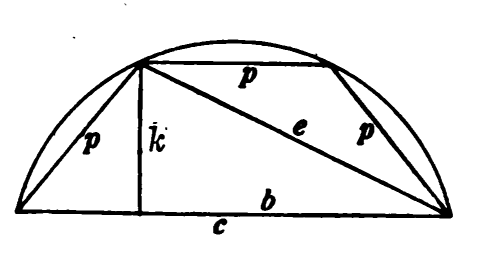
\includegraphics[width=0.6\linewidth]{pdf293-a.png}\end{center}
$e^2 = b^2 + k^2 = b^2 + \{p^2 - (c-b)^2\} = p^2 + cp$, or applying the formula for the 2-gonal line above obtained, we have $cd^2 - 3d^2p + 4p^3 = 0$, whence, writing $q = c^2/d^2$, $x = p^2/d^2$, follows
\[
-q + 9x - 24x^2 + 16x^3 = 0,
\]
and the \emph{tetsujutsu} expansion for the cubic gives
\[
p^2 = \frac{c^2}{9} + \frac{2.8q}{6.9}D_0 + \frac{5.14q}{9.15}D_1 + \frac{8.20q}{12.21}D_2 + \frac{11.36q}{15.27}D_3 + \cdots.
\]

\scanpage{0294}{printed page 280}
For the 4-gonal line the expansion for the 2-gonal line is taken and the resulting equation is subjected for a second expansion. We have thus
\[
p^2=\frac{c^2}{4^2}+\frac{3.5q}{6.8}D_0+\frac{7.9q}{10.12}D_1+\frac{11.13q}{14.16}D_2+\frac{15.17q}{18.20}D_3+\cdots.
\]

The ratio of the numerical coefficients of these three series are
\[
\begin{array}{lllllll}
\frac{1}{2^2}, & \frac{1.6}{4.6}, & \frac{3.10}{6.10}, & \frac{5.14}{8.14}, & \frac{7.18}{10.18}, & \frac{9.22}{12.22}, & \ldots,\\[1mm]
\frac{1}{3^2}, & \frac{2.8}{6.9}, & \frac{5.14}{9.15}, & \frac{8.20}{12.21}, & \frac{11.26}{15.27}, & \frac{14.32}{18.33}, & \ldots,\\[1mm]
\frac{1}{4^2}, & \frac{2.10}{8.12}, & \frac{7.18}{12.20}, & \frac{11.26}{16.28}, & \frac{15.34}{20.36}, & \frac{19.42}{24.44}, & \ldots.
\end{array}
\]

The laws of formation of these numbers are not difficult to be discovered. For in the first row the numbers
\[
1,\ 3,\ 5,\ 7,\ 9,\ \ldots;\ 4,\ 6,\ 8,\ 10,\ 12,\ \ldots;\ 6,\ 10,\ 14,\ 18,\ 22,\ \ldots
\]
proceed in arithmetical progressions, and it is the same with the rest of rows. Thus it will be found that the corresponding ratios for the $n$-gonal line are
\begin{gather*}
\frac{1}{n^2},\quad \frac{(1n-1).2(1n+1)}{2n.3n},\quad \frac{(2n-1).2(2n+1)}{3n.5n},\quad \frac{(3n-1).2(3n+1)}{4n.7n}\\
\frac{(4n-1).2(4n+1)}{5n.9n},\ \ldots,
\end{gather*}
or
\[
\frac{1}{n^2},\ \frac{2(1^2n^2-1)}{2.3n^2},\ \frac{2(2^2n^2-1)}{3.5n^2},\ \frac{2(3^2n^2-1)}{4.7n^2},\ \frac{2(4^2n^2-1)}{5.9n^2},\ \frac{2(5^2n^2-1)}{6.11n^2},\ \ldots.
\]

We have therefore for the $n$-gonal line,
\[
p^2=\frac{c^2}{n^2}+\frac{4q}{3.4}\left(1^2-\frac{1}{n^2}\right)D_0+\frac{4q}{5.6}\left(2^2-\frac{1}{n^2}\right)D_1+\frac{4q}{7.8}\left(3^2-\frac{1}{n^2}\right)D_2+\cdot\cdot
\]

If the method of the \emph{tetsujutsu} expansion is applied to this series, we have, on writing $\alpha=c^2/d^2$,
\[
p=\frac{c}{n}+\frac{\alpha}{2.3}\left(1^2-\frac{1}{n^2}\right)D_0+\frac{\alpha}{4.5}\left(2^2-\frac{1}{n^2}\right)D_1+\frac{\alpha}{6.7}\left(3^2-\frac{1}{n^2}\right)D_2+\cdots
\]

Next to find $c^2$ and $c$ in terms of $d$, $n$ and $p$, Hasegawa takes the expression obtained above in the form
\begin{multline*}
-n^2p^2+c^2+\frac{(1^2-\varkappa)c^4}{3d^2}+\frac{2(1^2-\varkappa)(2^2-\varkappa)c^6}{5.3^2d^4}+\frac{(1^2-\varkappa)(2^2-\varkappa)(3^2-\varkappa)c^8}{35.3^2d^6}\\
+\frac{(1^2-\varkappa)\ldots(4^2-\varkappa)c^{10}}{7.5^2.3^4d^8}+\frac{2(1^2-\varkappa)\ldots(5^2-\varkappa)c^{12}}{77.5^2.3^5d^{10}}+\cdots=0,
\end{multline*}
where $\varkappa=\frac{1}{n^2}$. This is an equation of degree infinite, from which we have to extract the value of $c^2$. Let it be required to find the first

\scanpage{0295}{printed page 281}
\noindent six terms in the expansion. Here we have only to retain the first powers of $c^2$ up to the 6th in the above series, for higher powers do not affect the required terms in the expansion. We have thus an equation of the 6th degree in $c^2$, a root of which is to be extracted by the \emph{tetsujutsu} method. We shall write this equation for simplicity's sake in the form\footnote{In Hasegawa's work it is given in a somewhat different form.},
\[
-t+x+\alpha x^2+\beta x^3+\gamma x^4+\delta x^5+\varepsilon x^6=0,
\]
which will be arranged in this scheme:\footnote{Here we employ the symbols $0^0$, $1^0$, $2^0$, \dots\ for the absolute and 1st, 2nd, \dots\ degree classes.}

\begin{center}
\begin{tabular}{|c|c|c|c|c|c|c|}
\hline
$0^0$ & $1^0$ & $2^0$ & $3^0$ & $4^0$ & $5^0$ & $6^0$ \\
\hline
$-t$ & $1$ & $\alpha$ & $\beta$ & $\gamma$ & $\delta$ & $\varepsilon$ \\
\hline
\end{tabular}
\end{center}

The first step is to take $-0^0\div 1^0=t$ as the first term in the required expansion, and to follow the same steps as in solving numerical equations by the celestial element method (for which see chapter 11). The expression that remains after the operation assumes the form:

\begin{center}
\begin{tabular}{|l|c|c|c|c|c|c|}
\hline
\multicolumn{1}{|c|}{$0^0$} & $1^0$ & $2^0$ & $3^0$ & $4^0$ & $5^0$ & $6^0$ \\
\hline
$(-t$ & $1$ & $\alpha$ & $\beta$ & $\gamma$ & $\delta$ & $\varepsilon$ \\
\quad$+t)$ & $+2\alpha\mathrm{t}$ & $+3\beta t$ & $+4\gamma t$ & $+5\delta t$ & $+6\varepsilon t$ & \\
$+\alpha t^2$ & $+3\beta t^2$ & $+6\gamma t^2$ & $+10\delta t^2$ & $+15\varepsilon t^2$ & & \\
$+\beta t^3$ & $+4\gamma t^3$ & $+10\delta t^3$ & $+20\varepsilon t^3$ & & & \\
$+\gamma t^4$ & $+5\delta t^4$ & $+15\varepsilon t^4$ & & & & \\
$+\delta t^5$ & $+6\varepsilon t^5$ & & & & & \\
$+\varepsilon t^6$ & & & & & & \\
\hline
\end{tabular}
\end{center}

The next term in the expansion will be given by the lowest term in $t$ in the absolute class divided by 1, which is the lowest term in the $1^0$ class, taken with the opposite sign. Then the same process as before is to be repeated, but some of the members may be neglected without affecting the result in our required expansion. The members that affect the coefficient of $t^6$ in the absolute term class are the first 5, 3 and 1 terms in $1^0$, $2^0$, $3^0$ classes. The remaining members

\scanpage{0296}{printed page 282}
\noindent may be all got rid of at once. Carrying out the operation in this simplified form, we obtain the following result:\footnote{Here we have omitted to write down $t$ and its powers for simplicity's sake, but the successive rows will be considered as multiplied by $t^0$, $t^1$, $t^2$, \dots\ respectively.}

\begin{center}
\begin{tabular}{|l|l|l|l|}
\hline
\multicolumn{1}{|c|}{$0^0$} & \multicolumn{1}{c|}{$1^0$} & \multicolumn{1}{c|}{$2^0$} & \multicolumn{1}{c|}{$3^0$}\\
\hline
$\phantom{+}0$ & $\phantom{+}1$ & $\phantom{+}\alpha$ & $\beta^*$\\
$+0$ & $+2\alpha$ & $+3\beta^*$ & \\
$+(\alpha-\alpha)$ & $+3\beta-2\alpha^2$ & $+6\gamma-\alpha\beta^*$ & \\
$+\beta-2\alpha^2$ & $+4\gamma-6\alpha\beta$ & & \\
$+\gamma-3\alpha\beta+\alpha^2$\, & $+5\delta-(6\alpha\gamma^2-\alpha^2\beta)^*$ & & \\
$+\delta-4\alpha\gamma+3\alpha^2\beta$ & & & \\
$+\varepsilon-5\alpha\delta+6\alpha^2\gamma-\alpha^3\beta$ & & & \\
\hline
\end{tabular}
\end{center}

The terms marked with asterisks are not needed in the next operation, so that these are not accounted in full. The third term of the expansion is taken $=(2\alpha^2-\beta)t^3$ in accordance with the same rule

\noindent
\begin{minipage}[t]{0.47\linewidth}\vspace{0pt}
\begin{tabular}{|l|l|l|}
\hline
\multicolumn{1}{|c|}{$0^0$} & \multicolumn{1}{c|}{$1^0$} & \multicolumn{1}{c|}{$2^0$}\\
\hline
 & $\phantom{+}1$ & $\alpha^*$\\
$\phantom{+}At^4$ & $+2\alpha t$ & \\
$+Bt^5$ & $+(3\beta-2\alpha^2)t^2$ & \\
$+Ct^6$ & $+Dt^{3*}$ & \\
\hline
\end{tabular}
\end{minipage}\hfill
\begin{minipage}[t]{0.5\linewidth}\vspace{0pt}
as done before. Effecting a similar operation as before we get the remaining expression in the form as annexed, where we write
\[
A=\gamma-3\alpha\beta+\alpha^3+(4\alpha^2-2\alpha\beta),
\]
\[
\begin{aligned}
B&=\delta-4\alpha\varepsilon+3\alpha^2\beta+(8\alpha^2\beta\\
&\qquad-3\beta^2-4\alpha^4),
\end{aligned}
\]
\end{minipage}
\[
\begin{gathered}
C=2-5\alpha\delta+6\alpha^2\gamma-\alpha^3\beta+(-4\beta\gamma-3\alpha^2\beta+8\alpha^2\gamma+7\alpha\beta^2+6\alpha^2\\
-14\alpha^3\beta),\\
D=4\gamma-6\alpha\beta+(3\alpha^2-\alpha\beta).
\end{gathered}
\]

\noindent
\begin{minipage}[t]{0.62\linewidth}\vspace{0pt}
\begin{tabular}{|l|c|}
\hline
\multicolumn{1}{|c|}{$0^0$} & $1^0$\\
\hline
$(A-A)t^4$ & $1$\\
$(+B-2\alpha A)t^5$ & $2\alpha t$\\
$\{+\gamma-(3\beta-2\alpha^2)A\}t^6$ & $(+3\beta-2\alpha^2)t^{2*}$\\
\hline
\end{tabular}
\end{minipage}\hfill
\begin{minipage}[t]{0.35\linewidth}\vspace{0pt}
\setlength{\parindent}{1.5em}
\indent The fourth term of the expansion is $-At^4$, and the operation goes as shown annexed.

The fifth term is $-(B-2\alpha A)t^5$, and
\end{minipage}

\noindent we obtain the following expression after the corresponding operation.

\scanpage{0297}{printed page 283}
\begin{center}
\begin{tabular}{|c|c|}
\hline
$0^0$ & $1^0$\\
\hline
$(B-2\alpha A)t^5-(B-2\alpha A)t^5$ & $1$\\
$+\{C-(3\beta-2\alpha^2)A-2\alpha(\beta-2\alpha A)\}t^6$ & $+\,2\alpha t$\\
\hline
\end{tabular}
\end{center}

The next and last term required will then obviously be
\[
\{-C+(3\beta-2\alpha^2)A+2\alpha(B-2\alpha A)\}t^6.
\]

Thus the result obtained is, after rewriting, of the form
\[
\begin{aligned}
c^2=p^2n^2&-\frac{4k}{3.4}(n^2-1^2)D_0+\frac{4k}{5.6}(n^2-2^2)D_1-\frac{4k}{7.8}(n^2-3^2)D_2\\
&+\frac{4k}{9.10}(n^2-4^2)D_3-\frac{4k}{11.12}(n^2-5^2)D_4+\cdots,
\end{aligned}
\]
where $k=p^2/d^2$.

The above is the way of reversion of series employed by the old Japanese mathematicians of a century ago.

If we apply the \emph{tetsujutsu} process to this series we obtain
\[
c=pn-\frac{k}{2.3}(n^2-1^2)D_0+\frac{k}{4.5}(n^2-3^2)D_1-\frac{k}{6.7}(n^2-5^2)D_2+\cdots
\]

What we have said in the above is applicable to the \emph{kakujutsu} or polygonal theory, one of important branches of the Japanese mathematics. Thus to find the square of the circumradius $r$ of the regular $n$-gon, Hasegawa proceeds as follows:\footnote{The procedure is only partially rigorous.} From what has been obtained we have
\[
\begin{aligned}
p^2=\frac{c^2}{n^2}&+\frac{4}{3.4}\left(1^2-\frac{1}{n^2}\right)\frac{c^2}{d^2}D_0+\frac{4}{5.6}\left(2^2-\frac{1}{n^2}\right)\frac{c^2}{d^2}D_1\\
&+\frac{4}{7.8}\left(3^2-\frac{1}{n^2}\right)\frac{c^2}{d^2}D_2+\cdots.
\end{aligned}
\]
Now the hexagon is the only polygon whose side bears a commensurable ratio to the diameter of the circum-circle. And so the author takes the hexagon for the purpose of his explanation. It will be seen that the side of an equilateral triangle is the chord of an arc to which six sides of a 18-gon are inscribed, that the side of a square is the chord of an arc to which six sides of a 24-gon are inscribed, that the side of a pentagon is the chord of an arc to which six sides of a 30-gon are inscribed, and so on. Hence if $m$ be the number of

\scanpage{0298}{printed page 284}
sides, $\frac{m}{b}$ is the number of equal chords inscribed within the arc of a side of the hexagon, which is $=\frac{d}{2}\cdot$ If therefore we take $c=\frac{1}{2}\,d$, we have $c^2/d^2=\frac{1}{4}$, and $1/n^2=6^2/m^2=k$, say. Thus the above series becomes
\[
\frac{p^2}{(\frac{1}{2}d)^2}=k+\frac{1^2-k}{3.4}\,k+\frac{2^2-k}{5.6}\,D_1+\frac{3^2-k}{7.8}\,D_2+\frac{4^2-k}{9.10}\,D_3+\cdots,
\]
whence follows $\left(\frac{d}{2}\right)^2=r^2=p^2/(\text{the series})$.

This reasoning has originally been attempted in the case of polygons whose number of sides is a multiple of 6. But the author has no hesitation to apply it to the general case without any further considerations. This was of course not the case only with our author; the Japanese mathematicians of the old school were ever accustomed with such looseness of reasoning. What they had aimed at was in the final results only; the preliminary considerations leading to these results were merely looked upon as instruments serving for the purpose.

The formula for the circum-radius $r$ of a regular $m$-gon was obtained to be
\[
r=p/\left\{\frac{6}{m}+\frac{(1^2-k)}{4.6}\,D_0+\frac{(3^2-k)}{8.10}\,D_1+\frac{(5^2-k)}{12.14}\,D_2+\cdots\right\},
\]
the same expression as obtained by Kurushima Yoshita.\footnote{Fukuda Riken's \emph{Sampō Tamatebako}, 1879.}

\begin{center}
CHAPTER 41.\\[1mm]
ON THE WEDGE-SECTIONS IN HASEGAWA'S\\
KYŪSEKI TSŪKŌ.
\end{center}
\phantomsection\addcontentsline{toc}{subsection}{Chapter 41. On the Wedge-Sections in Hasegawa's Kyūseki Tsūkō}

1. The best treatise on the circular theory was undoubtedly Hasegawa Kō's \emph{Kyūseki Tsūkō}. This was written by Hasegawa's hand but it was brought out in his pupil Uchida Kyūmei's name in 1844. The work contains a discussion on circular wedges, of which we shall attempt a description in the following lines.

The subject of the wedge was no new theme. Some of the problems in the ancient \emph{Chiu-chang} or \emph{Nine Sections} concerned it, being followed by various other writers. Japanese mathematicians of the 17th and 18th centuries also extensively studied allied subjects. Even wedges on circular bases were noticed before the publication of the treatise before us. But a systematic study of the subject was attempted for the first time in Hasegawa's work.

\scanpage{0299}{printed page 285}
2. Hasegawa treats circular wedges in two classes. The edge of a wedge may be of any length independent of the size of the base, but Hasegawa considers only the case for which the edge is equal to the diameter of the base circle, except in some special cases. The formation of such a wedge may be conceived in two ways, as he discusses.

Suppose the diameter of the base circle, which is parallel to the edge, be divided into a number of equal parts as the edge is divided. Drawing the ordinates at right angles to the diameter at these points of division, join the corresponding points of division of the circumference and of the edge by straight lines. If then the number of divisions be increased without limit, we get a surface, which is the circular wedge of one species.

The wedge of another species will be obtained when the divisions of the semi-circumference upon the said diameter are effected equally.

These circular wedges are called right when the diameter of reference and the edge form a rectangle, its plane being normal to that of the base. Oblique wedges may also be formed.

The base of a wedge may be replaced by an ellipse, by a circular segment or by plane curves of any form. The discussions of these wedges would be highly interesting, for they are far more complicated than in the case of the circular wedge.

Of the two species of wedges, the second is the one which is usually referred to as a wedge simply. Hasegawa calls this sort of the wedge the ``normal wedge'', while the other is called ``the abnormal''. He however mostly considers the latter species.

3. If the right circular or elliptic wedges of this species are cut by a plane parallel to the base, the section is an ellipse. The section by a plane normal to the diameter of reference (in the case of an elliptic wedge the major or minor diameter being understood) and through one end of the diameter and the opposite end of the wedge, is a curve called \emph{hōshu-yen} or ``\emph{hōshu}-formed circle or oval''. It was called in later years by the name \emph{senyen} or ``pointed circle or cusped oval''.

If the plane does not go through the end of the edge, but cuts the wedge along the generating line through that end, the form of the section is a curve resembling the ``cusped oval'' but not with a point or cusp.

The section that goes through a point on the edge is a curve also with a pointed end, which is however not a cusp in this case but a node.

\scanpage{0300}{printed page 286}
In the case of an oblique wedge the sections are also of the same forms, save that they are deformed owing to the obliqueness of the wedge.

Other kinds of sections may of course be formed, such for example as the section through the middle point of either semi-circumference or half perimeter divided by the diameter parallel to the edge.

4. The wedges considered in the following lines are, except in exceptional cases, all abnormal wedges. And therefore we shall for the sake of simplicity call the wedge of this description merely a wedge.

To find the area of a section parallel to the base of a circular wedge, Hasegawa proceeds in this way. Divide the diameter of the
\begin{center}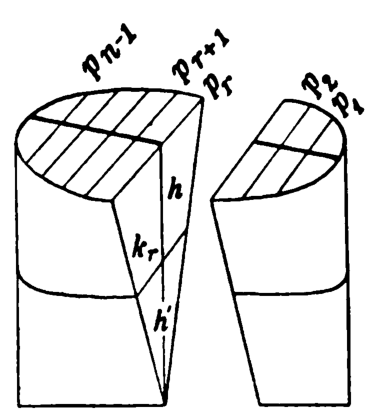
\includegraphics[width=0.6\linewidth]{pdf300-a.png}\end{center}
base into $n$ equal parts by parallel diameters $p_1$, $p_2$, $\ldots$, $p_{n-1}$, which are counted beginning at one end of the diameter. Construct the normal sections through these ordinates. Then designating the altitude of the wedge by $h$, that of the section by $h'$, the chord of the section plane corresponding to $p_r$ by $k_r$, the greatest value of $k_r$ (or the middle one) by $k$, we have
\[
h' = \frac{hk}{d}, \quad k_r = \frac{p_r h'}{h} = \frac{p_r k}{d},
\]
where $d$ is the diameter of the base parallel to the edge. Hence the element of area of the section is $A_r = k_r \times \frac{d}{n} = \frac{p_r k}{n}$, and consequently the area $A$ is
\[
A = \lim\nolimits_{n=\infty} \sum_{r=1}^{n} A_r = k \lim \sum_{r=1}^{n} \frac{p_r}{n} = \frac{kB}{d} = \frac{kd^2\frac{\pi}{4}}{d} = kd\frac{\pi}{4},
\]
where $B$ is the area of the base. But $kd\frac{\pi}{4}$ is the area of an ellipse with $k$ and $d$ as its principal diameters. Thus Hasegawa concludes that the section is an ellipse.

This consideration is equally applicable to the case of an elliptic wedge. In that case $d'$ being the diameter of the base normal to $d$, the value of $k$ will be found from $h' = hk/d'$, and thus $k_r = p_r k/d'$. Therefore the area of the section is to be taken
\[
= k \cdot \frac{d}{d'} \cdot \frac{B'}{d} = k \cdot \frac{d}{d'} \cdot \frac{dd'\frac{\pi}{4}}{d} = kd\frac{\pi}{4},
\]
where $B'$ is the area of the basic ellipse.

\scanpage{0301}{printed page 287 (top right)}
5. For the volume of the part of the wedge cut off by the section parallel to the base from the side of the edge, we have
\[
V_r = \frac{1}{2}\cdot k_r h'\cdot\frac{d}{n} = \frac{p_r h k^2}{2nd},
\]
\[
\therefore\quad V = \lim\nolimits_{n=\infty}\sum_{r=1}^{n} V_r = \lim\frac{hk^2}{2d}\sum_{r=1}^{n}\frac{p_r}{n} = \frac{hk^2}{2}\times\frac{\pi}{4}.
\]

If we write $k = d$ in this formula, we get the whole volume of a circular wedge to be $= \frac{hd^2}{2}\times\frac{\pi}{4}$.

\begin{center}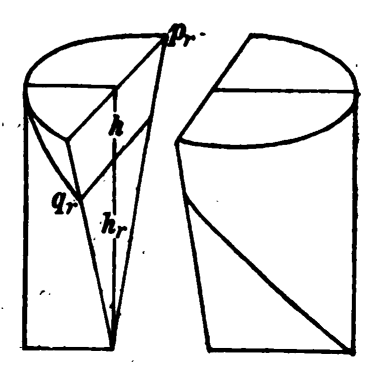
\includegraphics[width=0.6\linewidth]{pdf301-a.png}\end{center}

6. Next to find the volume of a part of the wedge cut off by a plane, which goes through one end of the edge and the opposite end of the diameter of the base parallel to it, and which is normal to the plane of these parallels, we have to try a construction similar to that in the previous case and designating as in the figure, the expressions for $h_r$ and $q_r$ are $h_r = \frac{h}{n}\times r$ and $q_r = \frac{p_r\times r}{n}$. Hence the element of volume is
\[
V_r = h_r q_r\times\frac{d}{n} = \frac{hp_r r^2 d}{n},
\]
\[
\therefore\quad V = hd\lim\sum\frac{p_r r^2}{n^3} = \frac{5hd^2}{32}\times\frac{\pi}{4}.
\]

7. The \emph{hōshuyen} is the curve arising from the section of a circular or elliptic wedge cut through an end-point of the diameter and the opposite end of the edge. The straight line joining these two end-points is called the vertical axis of the curve, while the axis normal to it at its middle way is called the lateral axis. This latter is, as is evident, of half the length of the diameter of the base conjugate to that which is parallel to the edge.

The calculation about the \emph{hōshuyen} is the same or similar, whether the base of the wedge be circular or elliptic.

Let the vertical and lateral axes of the curve be $a$ and $b$, respectively. Then in the construction as done in \S~6, $a$ will be divided into $n$ equal parts. Thus for the element of area of the curve we have
\[
A_r = q_r\times\frac{a}{n} = \frac{a\times r\times p_r}{n^2},
\]
\[
\therefore\quad A = a\lim\nolimits_{n=\infty}\sum_{r=1}^{n}\frac{rp_r}{n^2} = a\left(\frac{d}{2}\cdot\frac{\pi}{4}\right) = ab\,\frac{\pi}{4},
\]
as will be calculated by aid of a table.

\scanpage{0302}{printed page 288}
8. To find the area of the section through the end of the diameter of the base and the middle point of the edge, let the line joining these two points be $a$ and divide $a$ into $2n$ equal parts by the planes normal to the diameter. We designate the chords of the base obtained by these planes by $p_1, p_2, \ldots$ counting from the centre, and the lines drawn from the points of division of $a$ to the edge by $h_1, h_2, \ldots,$ and the chords of the section drawn parallel to $p_1, p_2, \ldots$ by $c_1, c_2, \ldots$. We have then
\begin{gather*}
A_r = \frac{a}{n} \times c_r = \frac{a}{n} \times \frac{p_r h_r}{h} = a \times \frac{r}{n^2} \times p_r,\\
\therefore\quad A = a \lim\nolimits_{n=\infty} \sum \frac{rp_r}{n^2} = \frac{ad}{3}.
\end{gather*}

9. In the case of a section that goes through the end of the diameter of the base and through a point of the generating line at the other end of the diameter, let $a$ be a similar length as before, and let $h'$ and $h_0$ be the two parts of the generating line, of which the former is adjacent to the base. We divide the diameter $d$ into $n$ equal parts by parallel planes, whose intersections with the base we call $p_r$, the number $r$ being counted from the generating line towards the other end of the diameter. Let $h_1, h_2, \ldots$ be the heights of the corresponding points of division of $a$, and let $k_r$ be the similar magnitudes as in the previous case. We have then $a = h'^2 + d^2$, and
\begin{gather*}
h_r = h_0 + \frac{rh'}{n}, \quad k_r = \frac{h_r p_r}{h} = \frac{h_0 p_r}{h} + \frac{rh' p_r}{nh}.\\
\therefore\quad A_r = k_r \times \frac{a}{n} = \frac{a}{h}\left(h_0 \times \frac{p_r}{n} + h' \times \frac{rp_r}{n^2}\right),\\
\therefore\quad A = \frac{a}{h}\left\{h_0 \lim\nolimits_{n=\infty} \sum_{r=1}^{n} \frac{p_r}{n} + h' \lim\nolimits_{n=\infty} \sum_{r=1}^{n} \frac{rp}{n^2}\right\}\\
= \frac{ad}{h}\left(h_0 + \frac{h'}{2}\right)\frac{\pi}{4} = \frac{ad}{h}\left(h - \frac{h'}{2}\right)\frac{\pi}{4}.
\end{gather*}

\begin{center}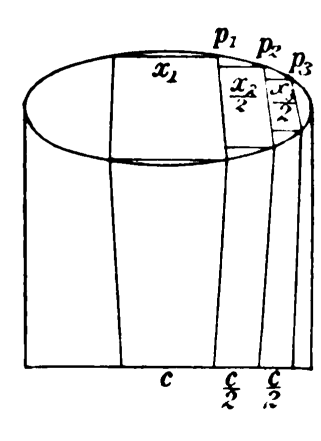
\includegraphics[width=0.6\linewidth]{pdf302-a.png}\end{center}

10. The circular wedges which arise from equal divisions of the circumference of the base circle are also considered. To find the volume of such a circular wedge, a construction is used as shown in the figure where half the semi-circumference of the base is divided into $2n$ equal parts. Draw the chords $p_1, p_2, \ldots$ from the points of division at right angles to the diameter of reference, the numbers being counted from the centre towards both sides. The chord joining the ends of the two equal chords $p_1$ is termed $x_1$, and the perpendicular

\scanpage{0303}{printed page 289 (top right)}
let fall on $p_1, p_2, \ldots$ from the ends of $p_2, p_3, \ldots$ respectively are termed $\frac{x_2}{2}, \frac{x_3}{2}, \cdots$. The edge being also divided into $2n$ equal parts, each part is equal to $d/2n = c/2$, say.

We take for the element of volume $V_r$ twice the volume of the rectilinear wedge with the base $p_r \times \frac{x_r}{2}$ and the edge $\frac{c}{2}$, the normal altitude being the same as that of the circular wedge, or $h$. Thus $V_r = \frac{1}{6}hp_r(2x_r + c)$.

\begin{center}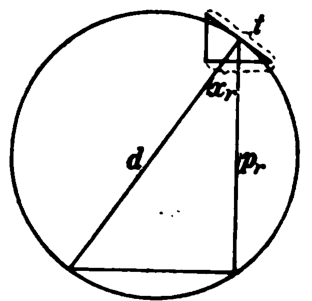
\includegraphics[width=0.6\linewidth]{pdf303-a.png}\end{center}

Now suppose a figure drawn as annexed. We have evidently
\[
p_r : d = x_r : t,
\]
or
\[
t = \frac{d\,x_r}{p_r}.
\]
But the equal parts (namely twice the parts we have divided) of the divisions of the circumference may be looked upon as the limiting value of $t$, so that we may write
\[
t = \frac{d\pi}{2} \times \frac{1}{n}, \quad\text{and}\quad \therefore\ c = \frac{d}{n} = \frac{2t}{\pi}.
\]

When we substitute these values of $c$ and $t$ in $V_r$, it becomes
\[
V_r = \frac{1}{6}hp_r\left(2x_r + \frac{2t}{\pi}\right) = \frac{1}{3}hx_r\left(p_r + \frac{d}{\pi}\right),
\]
whence the operation of folding or integration gives
\[
\begin{aligned}
V &= \frac{h}{3}\lim\nolimits_{n=\infty}\sum_{r=1}^{n} x_r p_r + \frac{hd}{3\pi}\lim\nolimits_{n=\infty}\sum_{r=1}^{n} x_r\\
&= \frac{h}{3}\left(d^2 \times \frac{\pi}{4}\right) + \frac{hd}{3\pi}(d) = \frac{hd^2}{3}\left(\frac{\pi}{4} + \frac{1}{\pi}\right).
\end{aligned}
\]

11. The area of a section of the circular wedge of this species cut parallel to the base is found as follows. For this purpose Hasegawa carries out the same construction as in \S~10, whereby the lenghts for the section corresponding to $p_r$ and $x_r$ in the base are denoted by $k_r$ and $y_r$ respectively. Let $h'$ be the normal distance of the section from the edge, and $k$ its diameter normal to the edge. Here we have
\[
d : p_r = k : k_r, \quad \therefore\ k_r = \frac{p_r k}{d}, \quad\text{and}\quad h' = \frac{hk}{d};
\]
and also
\[
(c - x_r) : (c - y_r) = h : h', \quad\text{or}\quad c - y_r = \frac{h'(c - x_r)}{h},
\]

\scanpage{0304}{printed page 290 (top left)}
\noindent whence we have
\[
y_r = c - \frac{h'(c-x_r)}{h} = c - \frac{ck}{d} + \frac{x_r k}{d}.
\]

Writing $c = 2t/\pi$, $tp_r = dx_r$, as in the last paragraph, we have for the element of area
\[
\begin{aligned}
A_r &= y_r k_r = \frac{kp_r}{d}\left(c - \frac{ck}{d} + \frac{x_r k}{d}\right) = \frac{2x_r k}{\pi} - \frac{2x_r k^2}{d\pi} + \frac{x_r p_r k^2}{d^2},\\
\therefore\ A &= \frac{2k}{\pi}\left(1 - \frac{k}{d}\right)\lim\nolimits_{n=\infty}\sum x_r + \frac{k^2}{d^2}\lim\nolimits_{n=\infty}\sum x_r p_r\\
&= \frac{2k}{\pi}(d-k) + \frac{k^2\pi}{4}.
\end{aligned}
\]

12. For the volume of the part of the wedge cut off by the section, the element is taken $=\frac{1}{6}h'k_r(2y_r + c)$ and consequently we have the volume
\[
V = \lim\nolimits_{n=\infty}\sum_{r=1}^{n}\frac{h'k_r}{6}(2y_r + c) = \frac{hk}{3}\left(\frac{k}{\pi} + \frac{A}{d}\right),
\]
where $A$ is the area of the section.

\begin{center}
CHAPTER 42.\\[1mm]
MAGIC SQUARES.
\end{center}
\phantomsection\addcontentsline{toc}{subsection}{Chapter 42. Magic Squares}

Magic squares and magic circles were stŭdied\unclear{stŭdied / stūdied / studied} in China, and we may mention, for instance, Ch'êng Tai-wei's \emph{Suan-fa T'ung-tsung} of 1593. This treatise was introduced into Japan and caused the uprise of mathematical studies. The Japanese too studied these subjects appareutly\unclear{appareutly / apparently} borrowing from the Chinese master.\footnote{See Smith and Mikami's \emph{History}. Something about the subject in the 17th century is described there.} The subject constituted one of the favourite themes for the Japanese mathematicians. We here propose to make a statement about one or two instances of the magic squares occurring in the 18th and 19th centuries.

The \emph{Kyūshi Ikō} or ``Kurushima's Posthumous Works'' contains a method of constructing odd magic squares. Taking $n^2$ to be the number of elements, the numbers $1$, $n^2$, $n$, $(n^2 + 1 - n)$ and $\frac{1}{2}(n^2 + 1)$ will be arranged as shown in the left one of the figures and we have to fill

\scanpage{0305}{printed page 291 (top right)}
the cells along the diagonal $CD$ by numbers that decrease towards $C$
and increase towards $D$ by successive multiples of $n$. The next step
\begin{center}
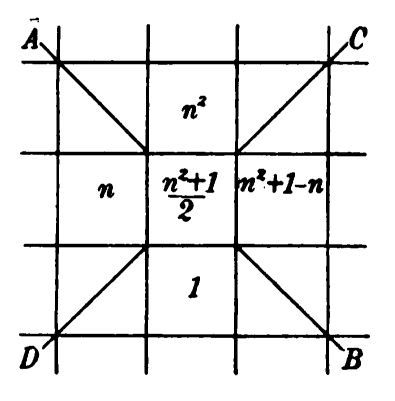
\includegraphics[width=0.3\linewidth]{pdf305-a.png}\qquad
\begin{tabular}[b]{|c|c|c|c|c|c|c|}
\hline
22 & 47 & 16 & 41 & 10 & 35 & 4\\ \hline
5 & 23 & 48 & 17 & 42 & 11 & 29\\ \hline
30 & 6 & 24 & 49 & 18 & 36 & 12\\ \hline
13 & 31 & 7 & 25 & 43 & 19 & 37\\ \hline
38 & 14 & 32 & 1 & 26 & 44 & 20\\ \hline
21 & 39 & 8 & 33 & 2 & 27 & 45\\ \hline
46 & 15 & 40 & 9 & 34 & 3 & 28\\ \hline
\end{tabular}
\end{center}
is to fill along the lines $n$ to $n^2$ and 1 to $(n^2+1-n)$ according to
the same law as along $CD$. Then the cells along the diagonal $AB$
and parallel to it will be filled decreasing and increasing by unity in
the directions of $A$ and $B$, respectively. The right one of the figures
represents a 7-square constructed in this manner.

Murai Chūzen's \emph{Sampō Dōshimon} of 1781 was the first occasion
of describing a general method for magic squares in a printed work,
the writings of his predecessors, Seki, Aoyama, Matsunaga, etc., being
all recorded only in manuscripts. We shall illustrate Murai's way of
constructing an odd square for the case of $5^2$ elements. Arrange the
number $\frac{n+1}{2}+1=3$ in the cells along one diagonal, and other numbers
increasing or decreasing by unity are to be arranged along the lines
parallel to this diagonal, as shown in the first of the accompanying
figures, where these numbers are represented in Roman numerals. The
same way of arrangement will be also done along another diagonal
and parallel to it, which we represent by Arabian numerals. The second
of the figures is an arrangement of natural numbers in a natural order
\begin{center}
\begin{tabular}[b]{|c|c|c|c|c|}
\hline
$\mathrm{IV}_3$ & $\mathrm{V}_2$ & $\mathrm{I}_1$ & $\mathrm{II}_5$ & $\mathrm{III}_4$\\ \hline
$\mathrm{V}_4$ & $\mathrm{I}_3$ & $\mathrm{II}_2$ & $\mathrm{III}_1$ & $\mathrm{IV}_5$\\ \hline
$\mathrm{I}_5$ & $\mathrm{II}_4$ & $\mathrm{III}_3$ & $\mathrm{IV}_2$ & $\mathrm{V}_1$\\ \hline
$\mathrm{II}_1$ & $\mathrm{III}_5$ & $\mathrm{IV}_4$ & $\mathrm{V}_3$ & $\mathrm{I}_2$\\ \hline
$\mathrm{III}_2$ & $\mathrm{IV}_1$ & $\mathrm{V}_5$ & $\mathrm{I}_4$ & $\mathrm{II}_3$\\ \hline
\end{tabular}\quad
\begin{tabular}[b]{c|c|c|c|c|c|}
\multicolumn{1}{c}{} & \multicolumn{1}{c}{1} & \multicolumn{1}{c}{2} & \multicolumn{1}{c}{3} & \multicolumn{1}{c}{4} & \multicolumn{1}{c}{5}\\ \cline{2-6}
1 & 1 & 6 & 11 & 16 & 21\\ \cline{2-6}
2 & 2 & 7 & 12 & 17 & 22\\ \cline{2-6}
3 & 3 & 8 & 13 & 18 & 23\\ \cline{2-6}
4 & 4 & 9 & 14 & 19 & 24\\ \cline{2-6}
5 & 5 & 10 & 15 & 20 & 25\\ \cline{2-6}
\end{tabular}\quad
\begin{tabular}[b]{|c|c|c|c|c|}
\hline
14 & 10 & 1 & 22 & 18\\ \hline
20 & 11 & 7 & 3 & 24\\ \hline
21 & 17 & 13 & 9 & 5\\ \hline
2 & 23 & 19 & 15 & 6\\ \hline
8 & 4 & 25 & 16 & 12\\ \hline
\end{tabular}
\end{center}

\scanpage{0306}{printed page 292 (top left)}
\noindent and we designate its rows and columns as represented there. Then we construct a third square whose cells we fill corresponding to those of the first square, in such a way that the elements in the second square with the numbers of rows and columns as indicated respectively by the Roman and Arabian numerals in the first square are used for the purpose. So for instance the cell of the third square, that corresponds to that in the first square marked III and 5, will be filled with the member 23 of the second square, which lies in the row 3 and the column 5. The square thus formed is magical as required. The same rule will be applicable to the case of any number of elements.

\begin{center}
\begin{tabular}{|c|c|c|c|}
\hline
$1_{\mathrm{IV}}$ & $2_{\mathrm{I}}$ & $3_{\mathrm{I}}$ & $4_{\mathrm{IV}}$ \\
\hline
$2_{\mathrm{III}}$ & $4_{\mathrm{II}}$ & $1_{\mathrm{II}}$ & $3_{\mathrm{III}}$ \\
\hline
$3_{\mathrm{II}}$ & $1_{\mathrm{III}}$ & $4_{\mathrm{III}}$ & $2_{\mathrm{II}}$ \\
\hline
$4_{\mathrm{I}}$ & $3_{\mathrm{IV}}$ & $2_{\mathrm{IV}}$ & $1_{\mathrm{I}}$ \\
\hline
\end{tabular}
\end{center}

For even squares Murai gives only an example, where the arrangement as shown in the figure is indicated without any explanation. But when we compare it with the explanation in the case of an odd square, the law of construction will be obvious.

Gokai Ampon's \emph{Sampō Semmon-shō} of 1840 treats also of a mode of constructing magic squares. He considers them classified into three kinds, odd, doubly even and simply even. To construct an odd square, Gokai places the unity in the cell one position below the central one and proceeds from that
\begin{center}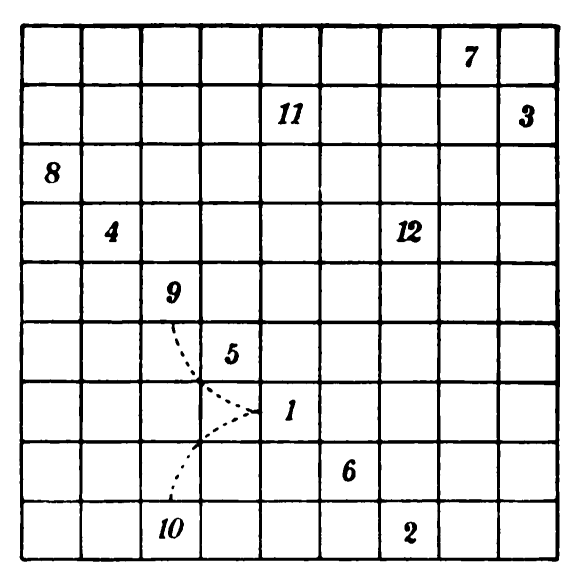
\includegraphics[width=0.6\linewidth]{pdf306-a.png}\end{center}
along the diagonal line leading to the right under side, filling the cells by the numbers 2, 3, \dots. When we come however to a position along the line at bottom or along the right side, it will be passed over to the topmost cell in the next vertical line or to the leftmost cell in the next horizontal line, and continued in the same way. When in this way we come to a cell already filled, we have to go to the cell next to it at the left under side. The same construction may also be adopted, if we place unity in the cell two or more positions below the central one. In this case every time the same number of positions is to be passed over in the procedure. The annexed figure may illustrate the nature of the construction.

To construct a doubly even square with $(4n)^2$ elements, it is considered to consist of a number of 4-squares. Suppose in these elementary 4-squares the diagonals drawn. Then arranging the first $(4n)^2$

\scanpage{0307}{printed page 293}
\noindent natural numbers in the two schemes as annexed, fill the cells of a square with the corresponding members of the first of these aggregates

\begin{center}
\begin{tabular}{|cccc|}
\hline
1 & $4n+1$ & $2.4n+1$ & . \\
2 & $4n+2$ & $2.4n+2$ & $\vdots$ \\
$\vdots$ & $\vdots$ & $\vdots$ & $\vdots$ \\
$4n$ & $2.4n$ & $3.4n$ & $\vdots$ \\
\hline
\end{tabular}
\qquad\qquad
\begin{tabular}{|cccc|}
\hline
$\vdots$ & $3.4n$ & $2.4n$ & $4n$ \\
$\vdots$ & $\vdots$ & $\vdots$ & $\vdots$ \\
$\vdots$ & $2.4n+2$ & $4n+2$ & 2 \\
. & $2.4n+1$ & $4n+1$ & 1 \\
\hline
\end{tabular}
\end{center}

\noindent that come under the diagonal lines just mentioned and with those of the second that do not come under such lines. The result is a magic square.

For the construction of simply even squares, Gokai first draws such figures as annexed and fills the cells along the diagonals in an

\begin{center}
\begin{minipage}[b]{0.18\linewidth}\centering
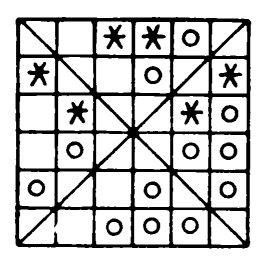
\includegraphics[width=\linewidth]{pdf307-a.png}\\
{\small $6^2$-square.}
\end{minipage}\hfill
\begin{minipage}[b]{0.28\linewidth}\centering
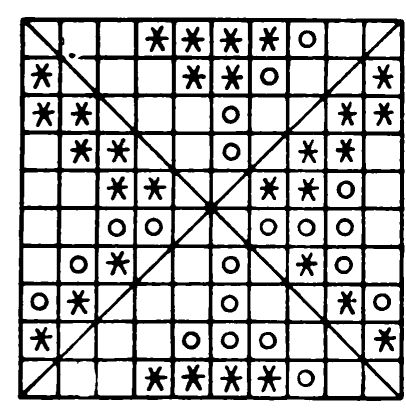
\includegraphics[width=\linewidth]{pdf307-b.png}\\
{\small $10^2$-square.}
\end{minipage}\hfill
\begin{minipage}[b]{0.40\linewidth}\centering
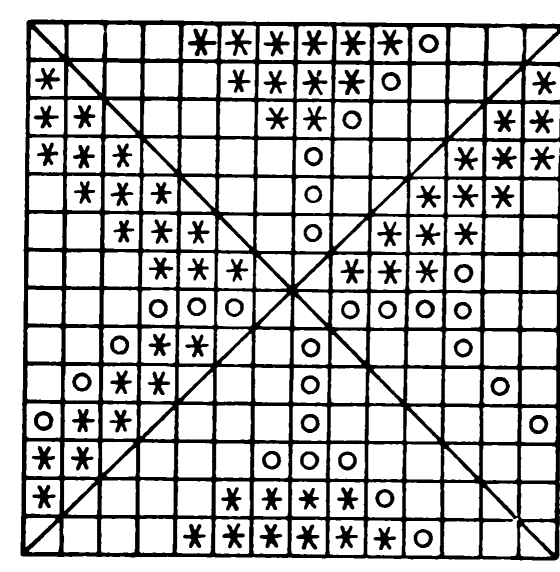
\includegraphics[width=\linewidth]{pdf307-c.png}\\
{\small $14^2$-square.}
\end{minipage}
\end{center}

\noindent order similar to the first of the above aggregates in the case of a doubly even square and fills the cells marked with circles in the same manner as in the second of the aggregates. Then taking the two

\begin{center}
\begin{tabular}{|cccc|}
\hline
$\vdots$ & $\vdots$ & $\vdots$ & $\vdots$ \\
2 & $m+2$ & $2m+2$ & $\vdots$ \\
1 & $m+1$ & $2m+1$ & $\vdots$ \\
\hline
\end{tabular}
\qquad\qquad
\begin{tabular}{|cccc|}
\hline
$\vdots$ & $2m+1$ & $m+1$ & 1 \\
$\vdots$ & $2m+2$ & $m+2$ & 2 \\
$\vdots$ & $\vdots$ & $\vdots$ & $\vdots$ \\
\hline
\end{tabular}
\end{center}

\noindent arrangements as shown here, where we understand by $m$ the number of cells in one side, the cells marked with asterisks (originally black circles) are to be filled by corresponding members of the 1st of these arrangements, while the remaining cells are to be filled by those of the second.

\scanpage{0308}{printed page 294 (top left)}
\begin{center}
CHAPTER 43.\\[1mm]
THE CATENARY.
\end{center}
\phantomsection\addcontentsline{toc}{subsection}{Chapter 43. The Catenary}

1. The first appearance of problems concerning the catenary in a Japanese work was perhaps in the \emph{Sūri Shimpen}, Book 2, published in 1860 by Yasuhara and Nakasone. The catenary was called \emph{suishi} or ``hanging string'' in Japan. The work here mentioned contains a problem of finding the length of the sagitta\footnote{Here we employ the term sagitta --- \emph{shi} or \emph{ya} in Japanese --- according to the usage followed by the Japanese mathematicians of the old school. In the case of a catenary the word \emph{suishi} or ``hanging sagitta`` was also used. Its meaning will be obvious, being the altidude of the curve.} of a catenary, whose length and the distance apart of whose two end-points are given. Here the problem is solved by a consideration resulting from the treatment of an ellipsé. This way of solution was a very rude one.\footnote{C. Kawakita's note to Ōmura's \emph{Suishi Kigen}.}

In 1862 Hagiwara Teisuke published the \emph{Sampō Hōyen-kan}, in which he gave the problem of finding the length of the hanging sagitta of a catenary, which is hung between two equal heights, being given the length of the curve. Writing the distance of the two ends $= a$, and the sagitta of the catenary $= b$, the rule given by Hagiwara for solution is equivalent to the series:
\[
\begin{gathered}
\frac{1}{6s}\Bigl[(s+a)\sqrt{s^2-a^2}+\frac{(s-a)^2}{2}+\frac{1}{3a}\Bigl\{D_0-(s-a)^3\\
+(1-m)\Bigl(D_0-\frac{1}{5}\,m\,D_1-\frac{1}{7}\,m\,D_2-\frac{3}{9}\text{}\,m\,D_3-\frac{5}{11}\,n\,D_4-\ldots\Bigr)\Bigr\}\Bigr],
\end{gathered}
\]
where $D_0=(s^2-a^2)\sqrt{s^2-a^2}$, $m=\frac{s-a}{s+a}$, and where $D_0$ and $D_1, D_2, \ldots$ represent the original term and the successive differences. Hagiwara's solution was given without explanation.

2. Some time after the publication of Hagiwara's work, Ōmura Isshū wrote the manuscript \emph{Suishi Kigen}, in which he embodied the results of his studies on the catenary. His work bears the date of the 6th month of 1867. In the 2nd month of 1868 Ōmura and Kagami Mitsuteru effected further studies. We give some of these results in the following lines:\footnote{C. Kawakita's copy of the \emph{Suishi Kigen}, dated 1874.}

To find the sagitta $b$ of a catenary in terms of the distance $a$ between the two end-points and the length $s$ of the curve, Ōmura draws

\scanpage{0309}{printed page 295}
\noindent a figure as annexed. Here the ordinates are drawn at equal intervals $\left(\frac{1}{2}\,l = a/2n\right)$, and the horizontal parallels are taken at such distances that the lengths indicated in the figure by $k_1$, $k_2$, \dots\ have the values
\begin{center}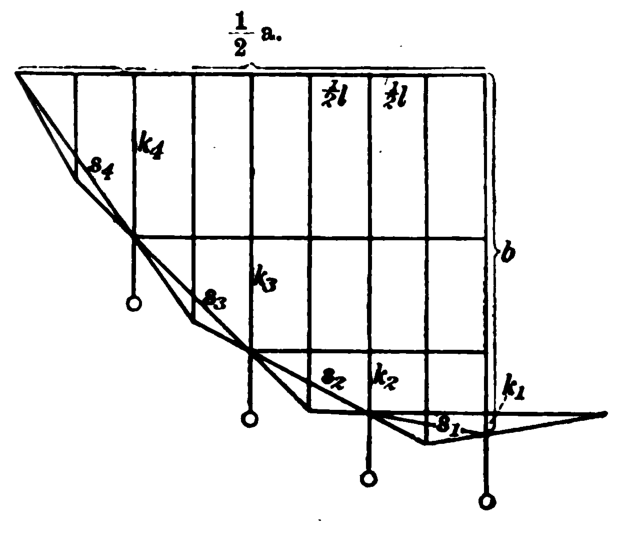
\includegraphics[width=0.6\linewidth]{pdf309-a.png}\end{center}
\[
\begin{gathered}
k_1 = k = \frac{b}{n^2},\quad k_r = (2r-1)\,k = \frac{2rb}{n^2} - \frac{b}{n^2}\\
= \frac{2bt}{n} - \frac{b}{n^2},
\end{gathered}
\]
where $t = r/n$. Here the second term may be neglected as it does not affect the result in the end, so that we may write $k_r = 2bt/n^2$. We have for the square of the element of arc
\[
s_r^2 = k_r^2 + l^2 = \frac{4b^2t^2}{n^2} + \frac{a^2}{4n^2} = \frac{pa^2}{4n^2}\left\{1 - (1-t^2)\,q\right\},
\]
\[
\text{or}\quad s_r = \frac{a\sqrt{p}}{2n}\left\{1 - \frac{(1-t^2)}{2}\,q - \frac{(1-t^2)^2}{8}\,q^2 - \frac{3(1-t^2)^3}{48}\,q^3 - \frac{15(1-t^2)^4}{384}\,q^4 - \cdots\right\},
\]
where we have written $p = \frac{16b^2}{a^2} + 1$, $q = \frac{16b^2}{a^2}\Big/p$. Now carrying out the operation of folding, namely summing and going to limit, we obtain, after doubling the result,
\[
s = 2\lim\nolimits_{n=\infty}\sum_{r=1}^{n} s_r = a\sqrt{p}\left(1 - \frac{q}{3} - \frac{q^2}{15} - \frac{q^3}{35} - \frac{q^4}{63} - \,..\right).
\]

The value of $b$ may be obtained from this expression by the application of the \emph{kanrui jutsu} or the method of recurring approximations. Thus substituting $b' = \frac{1}{2}\sqrt{s^2 - a^2}$ for $b$ in the above formula, let $s'$ be the value that corresponds to $s$. Then $\frac{1}{2}(s' - s)$ will be $< b' - b$, and will be nearly $= b' - b$, so that $b' - \frac{1}{2}(s' - s) \equiv b''$ is $> b$.

Next find the value of $s''$ in like way with $b''$, and so on, until two successive values of $s^{(i)}$ agree with each other. This coincident value will represent the length of the sagitta required.\footnote{The approximation method called the \emph{kanrui-jutsu} is usually believed to have been established by Saitō Gichō and first given in his \emph{Sampō Yenri-kan} of 1834. It is a process to be applied to the solution of a transcendental equation. We are however uncertain whether Wada Nei had been possessed of it before Saitō or not. This point is to be studied in the future.}

3. Supposing the two end-points of a catenary to lie horizontally, let the distance between these end-points be $a$, the length of the

\scanpage{0310}{printed page 296}
sagitta being $b$. Then suppose a horizontal chord is drawn, whose length is $a'$. What will be the length $b'$ of the part of the sagitta cut off by this horizontal chord?

To calculate this length Ōmura makes a construction iu like way as in the former case, and takes the $i$th ordinate counted from the sagitta to go through the end of the chord. Then adopting the same notations as above, we have
\[
b' = k + 3k + 5k + \ldots + (2i-1)k = i^2k = i^2b/n^2,
\]
\[
\text{but}\qquad a' = 2i\left(\frac{a}{2n}\right) = \frac{ia}{n}, \qquad \therefore\ b' = b \times \frac{a'^2}{a^2}.
\]

4. The length of a catenary hung between two points not of equal height may also be found. Thus let $A$, $B$, $C$ be the ordinates of the two end-points and of the lowest point of the curve, and let $a$ be the horizontal distance of the two ends. The horizontal chords should be constructed at the two ends. Denote these by $x$ and $x'$. We have then (the second formula being the result of the last paragraph)
\[
x' = 2a - x \quad\text{and}\quad (B-C)x^2 = (A-C)x'^2,
\]
\[
\therefore\quad \frac{x}{2} = \frac{a}{m+1} \quad\text{and}\quad \frac{x'}{2} = \frac{ma}{m+1}, \quad\text{where } m^2 = \frac{(B-C)}{A-C}.
\]

With these values we may proceed as tried in the above and obtain the expressions for the lengths of the catenary with these two chords. Half the sum will afford the length required. Thus it is equal to
\begin{multline*}
\sqrt{(A-C)^2 + \left\{\frac{a}{2(m+1)}\right\}^2} + m\sqrt{(A-C)(B-C) + \left\{\frac{a}{2(m+1)}\right\}^2} + \\
+ \frac{1}{A-C}\left\{\frac{a}{2(m+1)}\right\}^2 \sqrt{k}\left(1 - \frac{k}{3} - \frac{k^2}{5} - \frac{k^3}{7} - \ldots\right),
\end{multline*}
where
\[
k = \frac{(A-C)^2\left[m\sqrt{(A-C)^2 + \left\{\frac{a}{2(m+1)}\right\}^2} + \sqrt{(A-C)(B-C) + \left\{\frac{a}{2(m+1)}\right\}^2}\right]}{\left\{\frac{a}{2(m+1)}\right\}^2 + (A-C)^2\left[m\sqrt{(A-C)^2 + \left\{\frac{a}{2(m+1)}\right\}^2} + \sqrt{(A-C)(B-C) + \left\{\frac{a}{2(m+1)}\right\}^2}\right]}.
\]

5. We shall next describe Ōmura aud Kagami's studies for finding the chord of a catenary in terms of its length and sagitta.

Suppose two weights $W_1$ and $W_2$ are suspended from the trisection points of a string. Here a figure as annexed is given, where $B_1K$ and $B_2K$ represent the components of the weights, while the point $K$ is indicated thus: ``This point is the centre of gravity of the

\scanpage{0311}{printed page 297}
larger weight and the smaller weight. The right and left components of weight are directed towards the centre of gravity''. The figure is accompanied by the following principle: ``If, as in the figure, (the length) $A_1$ be obtained in correspondence to the larger weight, then $A_2$ should necessarily be obtained in correspondence to the smaller weight. This is the same as with the lever''.

\begin{center}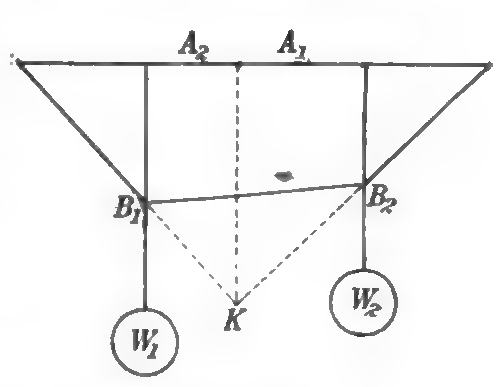
\includegraphics[width=0.6\linewidth]{pdf311-a.png}\end{center}

Here the division of the length is obviously intended in the proportion inverse to the weights. This principle is given in an axiomatical way.

In the consideration of the catenary the authors assume that equal weights are suspended at equal intervals, when the parts of the string between these weights are taken to be tightly stretched. Since now the weights are assumed to be equal, the centres of gravity of each successive two comes always midway between them. ``Thus arises the theory of the catenary'', it is added, ``from such a consideration. If then we consider the string divided in equal parts by suspended weights, we shall obtain the actual form of the catenary, when we go to the limit where the number of suspended weights becomes infinite.''

\begin{center}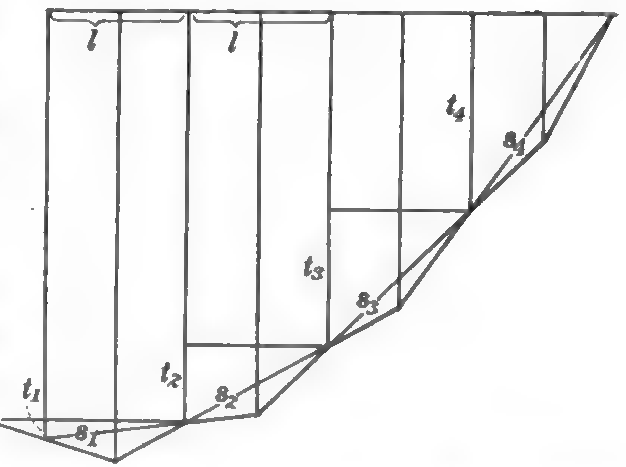
\includegraphics[width=0.6\linewidth]{pdf311-b.png}\end{center}

For the purpose of calculating the catenary the authors employ two sorts of figures. In one of these figures $n$ ordinates are drawn at one side of the sagitta at equal intervals $l$. The chords successively joining the ends of these ordinates are called the first, second, \dots, chords, which we denote by $s_1$, $s_2$, \dots.

Now from the ends of the ordinates horizontal lines are drawn towards the respective previous ordinates, from which they cut off the parts $t_1$, $t_2$, $t_3$, \dots, which are of the lengths:
\[
t_1 = t, \quad t_2 = 3t, \quad t_3 = 5t, \quad t_4 = 7t, \dots.
\]

Write $s_1 = s$, and $m = t_1{}^2/s^2$, then we have $l^2 = s^2 - t^2$, or expanded,
\[
l = s\left(1 - \frac{m}{2} - \frac{m^2}{8} - \frac{3m^3}{48} - \frac{15m^4}{384} - \cdots\right).
\]
We have also $\Bigl[$writing $p_r = 8 \cdot \frac{1}{2} r(r-1)\Bigr]$

\scanpage{0312}{printed page 298 (top left)}
\[
s_r^2 = (2r-1)^2 t^2 + l^2 = s^2 + \{(2r-1)^2 - 1\}\, t^2 = s^2 + 8\cdot\frac{r(r-1)}{2}\, t^2,
\]
\[
\therefore\quad \frac{s}{s_r} = 1 + \sum_{i=1}^{\infty} (-1)^i\, \frac{1.3.5\ldots(2i-1)}{2.4.6\ldots(2i)}\, p_r^i m^i.
\]

Next another figure is constructed in like way with the only difference that the 1st, 2nd, \dots{} chords, or $s_r$, are all made equal to $s = s_1$. Superposing this figure upon the former, so that the sagittae of the two figures become coincident, and so also the two chords $s_1$, the second chord of the second figure will partly coincide with the $s_2$ of the first figure, and the successive chords of the second figure take positions parallel respectively to $s_3$, $s_4$, \dots{} of the first figure, the result being as shown annexed.

\begin{center}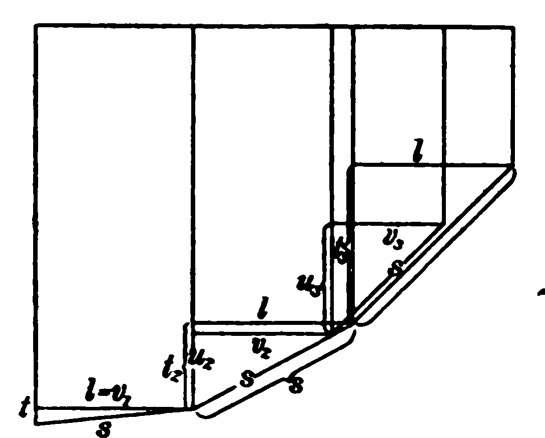
\includegraphics[width=0.6\linewidth]{pdf312-a.png}\end{center}

Here by the similarity of triangles we have
\[
t_r : u_r = s_r : s, \qquad \therefore\quad u_r = \frac{t_r s}{s_r} = \frac{(2r-1)\,t s}{s_r},
\]
whence, writing the sagitta $= b$, follows by summation
\[
\frac{b}{t} = \sum_{r=1}^{n} \frac{u_r}{t} = \sum_{r=1}^{n} \frac{(2r-1)\,s}{s_r} = \sum_{r=1}^{n} (2r-1) \left\{ 1 + \sum_{i=1}^{\infty} (-1)^i\, \frac{1.3.5\ldots(2i-1)}{2.4.6\ldots(2i)}\, p_r^i m^i \right\},
\]
\[
\begin{array}{r@{\;}r@{\;}r@{\;}r@{\;}r@{\;}l}
\therefore\quad \dfrac{b}{s\sqrt{m}} = n^2 & {}- n^4 m & {}+ 2n^6 m^2 & {}- 3\cdot\frac{5}{3}\, n^8 m^3 & {}+ 14 n^{10} m^4 & {}- \cdots \\[1mm]
 & {}+ n^2 m & {}- 4n^4 m^2 & {}+ 10\cdot\frac{5}{3}\, n^6 m^3 & {}- 70\, n^8 m^4 & {}+ \cdots \\[1mm]
 & & {}+ 2n^2 m^2 & {}- 11\cdot\frac{5}{3}\, n^4 m^3 & {}+ 29\cdot\frac{1}{3}\, n^6 m^4 & {}- \cdots \\[1mm]
 & & & {}+ 4\cdot\frac{5}{3}\, n^2 m^3 & {}- 175\cdot\frac{1}{3}\, n^4 m^4 & {}+ \cdots \\[1mm]
 & & & & {}+ 112\cdot\frac{1}{3}\, n^2 m^4 & {}- \cdots \\[1mm]
 & & & & & {}+ \cdots
\end{array}
\]

This may be considered as an equation for $\sqrt{m} = t/s$. If we write $n\sqrt{m} = x$, it will assume the form\footnote{The slight disagreement in the coefficients of these two expressions is certainly due to the fault of transcription.}

\scanpage{0313}{printed page 299}
\[
\begin{array}{@{}r@{}l|l@{}l|l@{}l|l@{}l|l@{}}
-\frac{b}{ns}+x & {}-1 & x^3 & {}+2 & x^5 & {}-5 & x^7 & {}+14 & x^9-\cdots=0.\\[2pt]
 & {}+\frac{1}{n} & & {}-\frac{4}{n^2} & & {}+\frac{50}{3n^2} & & {}-\frac{70}{n^2} & \\[2pt]
 & \multicolumn{1}{l}{} & & {}+\frac{2}{n^4} & & {}-\frac{55}{3n^4} & & {}+\frac{406}{3n^4} & \\[2pt]
 & \multicolumn{1}{l}{} & & \multicolumn{1}{l}{} & & {}+\frac{20}{3n^6} & & {}-\frac{350}{3n^6} & \\[2pt]
 & \multicolumn{1}{l}{} & & \multicolumn{1}{l}{} & & \multicolumn{1}{l}{} & & {}+\frac{112}{3n^8} &
\end{array}
\]

In the limit $n=\infty$, the quantity $sn$ becomes $=$ half the length of the catenary. Hence writing $b\div\text{(this length)}=a$, and neglecting $1/n$ and its powers, we obtain the equation
\[
-a+x-x^3+2x^5-5x^7+14x^9-\cdots=0,
\]
whence, the expansion by the \emph{tetsu-jutsu} method being applied, we get
\[
n\sqrt{m}=a+a^3+a^5+a^7+\cdots=a/(1-a^2).
\]

Again, writing the horizontal chord $=c$, we have from the above figure by proportion
\[
s_r:s=l:v_r,\quad\therefore\quad v_r=\frac{3l}{s_r},
\]
\begin{align*}
\therefore\ \frac{\frac{1}{2}c}{l}&=\frac{1}{l}\sum_{r=1}^{n}v_r=\sum_{r=1}^{n}\frac{s}{s_r}=n+\sum_{r=1}^{n}\sum_{i=1}^{\infty}(-1)^i\frac{1.3.5\ldots(2i-1)}{2.4.6\ldots(2i)}p_r{}^i m^i\\
&=n+\sum_{i=1}^{\infty}(-1)^i\frac{1.3.5\ldots(2i-1)}{2.4.6\ldots(2i)}m^i\sum_{r=1}^{n}p_r{}^i
\end{align*}
\[
\begin{array}{@{}r@{}l|l@{}l|l@{}l|l@{}l|l@{}}
=n & {}-n^3 & \frac{4}{3.2}m & {}+3n^5 & \frac{16}{5.8}m^2 & {}-15n^7 & \frac{64}{7.48}m^3 & {}+105n^9 & \frac{256}{9.384}m^4+\cdots\\[2pt]
 & {}+n & & {}-5n^3 & & {}+42n^5 & & {}-450n^7 & \\
 & \multicolumn{1}{l}{} & & {}+2n & & {}-35n^3 & & {}+693n^5 & \\
 & \multicolumn{1}{l}{} & & \multicolumn{1}{l}{} & & {}+\phantom{0}8n & & {}-420n^3 & \\
 & \multicolumn{1}{l}{} & & \multicolumn{1}{l}{} & & \multicolumn{1}{l}{} & & {}+\phantom{0}72n &
\end{array}
\]
$=n+A_1m+A_2m^2+A_3m^3+\cdots$, say.

If we now substitute for $l$ its expansion, we get after multiplication\footnote{The factors $\frac{1}{2}$, $\frac{1}{8}$, $\frac{3}{48}$, $\cdots$ are here indicated as to be multiplied into all the terms in the respective horizontal lines.}

\scanpage{0314}{printed page 300}
\[
\begin{array}{r@{}l|l@{}l|l@{}l|l@{}l|l}
\dfrac{\frac{1}{2}c}{s} = n & {}+ A_1 & m & {}+ A_2 & m^2 & {}+ A_3 & m^3 & {}+ A_4 & m^4 + \cdots\\[1ex]
\frac{1}{2}\cdots & {}- n & & {}- A_1 & & {}- A_2 & & {}- A_3 & \\[1ex]
 & \multicolumn{1}{l}{} & \frac{1}{8}\cdots & {}- n & & {}- A_1 & & {}- A_2 & \\[1ex]
 & \multicolumn{1}{l}{} & & \multicolumn{2}{r@{}}{\frac{3}{48}\;\cdots\cdots} & {}- n & & {}- A_1 & \\[1ex]
 & \multicolumn{1}{l}{} & & \multicolumn{1}{l}{} & & \multicolumn{2}{r@{}}{\frac{15}{384}\;\cdots\cdots} & {}- n &
\end{array}
\]

Here the $A$'s being replaced by their respective values and writing $4mn^2 = k$, we have
\[
\begin{array}{r@{}l|l@{}l|l@{}l|l}
\dfrac{\frac{1}{2}c}{ns} = 1 & {}- \dfrac{1}{3.2} & k & {}- \dfrac{3}{5.8} & k^2 & {}- \dfrac{15}{7.48} & k^3 - \cdots.\\[2ex]
 & {}+ \dfrac{1}{3.2n^2} & & {}- \dfrac{5}{48n^2} & & {}+ \dfrac{37}{320n^2} & \\[2ex]
 & \multicolumn{1}{l}{} & & {}+ \dfrac{41}{15.128n^4} & & {}- \dfrac{387}{3840n^4} & \\[2ex]
 & \multicolumn{1}{l}{} & & \multicolumn{1}{l}{} & & {}+ \dfrac{1643}{107520n^6} &
\end{array}
\]

Now going to the limit $n = \infty$, $ns$ becomes $= \frac{1}{2}$ (length of catenary) $= \frac{1}{2}S$, and neglecting the terms containing $1/n$ and its powers, we have
\[
\frac{c}{S} = 1 - \frac{k}{3.2} - \frac{3\,k^2}{5.8} - \frac{15\,k^3}{7.48} - \frac{105\,k^4}{9.384} - \cdots.
\]

Here $k = 4mn^2 = 4a^2/(1 - a^2)^2$, as we have given before, so that the powers of the expansion of $k$ being substituted in the above formula we have
\[
\frac{c}{S} = 1 - \frac{2\,a^2}{3} - \frac{2.1\,a^4}{15} - \frac{2.3\,a^6}{105} - \frac{2.15\,a^8}{945} - \cdots,
\]
where $a = 2b/S$.\footnote{It will be easily noticed that the above analysis given by Ōmura and Kagami is not very exact. The authors have sometimes put
\begin{center}
\begin{tabular}{@{}l@{}l@{}}
$\lim_{n=\infty} n\times s$ & ${}={}$ half the length of the catenary,\\
$\lim_{n=\infty} n\times u_r$ & ${}={}$ the sagitta of the catenary;
\end{tabular}
\end{center}
but there is no vouch for the legitimacy of these relations. The truth of the final result is therefore uncertain. This way of inexactness is, however, not rare among the productions of the Japanese mind, which has lacked in the scientific precission.}

\scanpage{0315}{printed page 301}
\begin{center}
CHAPTER 44.\\[1mm]
HAGIWARA TEISUKE.
\end{center}
\phantomsection\addcontentsline{toc}{subsection}{Chapter 44. Hagiwara Teisuke}

1. The last great mathematician belonging to the old Japanese school was certainly Hagiwara Teisuke. He contributed very much to the progress of the school during its closing days, and he may safely be taken for the best representative of his contemporary old school mathematicians, so that we have to say something about his life and works in this place. Besides, I knew the man when he lived. By actual conversation I have gathered much concerning his ideas. The impressions left by him upon my mind have ever remained, and will always continue to remain, with a vivid image in my memory. He was very old when I first saw him, and he told me that he had neglected his studies of mathematics for a score of years, being disappointed by the all-pervading influence of the Occidental mode of learning. He would not, however, concede anything to the superiority of his antagonist school. He insisted upon his belief of the inability of the Occidental mathematics to solve such complicated problems as had been studied by him. The wonderfully skillful devices of the old school alone had been helpful to lead him to the satisfactory solutions of these unwieldy questions. In the later days of his active studies he was indeed brought in contact with the integral calculus but his knowledge of it was of a vulgar and undigested kind; for he was learned in no European language and there had been no satisfactory translations of Occidental works in those days in all Japan. The Chinese translation of Loomis was perhaps the best source of information he could avail himself of. When we reflect on these circumstances we sympathise with his attitude. About the actual state of mathematical development in the West he had known nothing. He knew not even the progress of the Western science cultivated by his own countrymen in his old days. When I told him that these problems could be attacked by applying the integral calculus from such and such stand-points, he would only nod with a smile. I must say, I could not convince him of the greatness of the science at present, greater than the highest attainment of the old Japanese mathematics as developed in his hand. He died therefore with the mistaken but firm conviction that his results were the best artistic productions ever designed by the human hand or mind in the domain of mathem-

\scanpage{0316}{printed page 302 (top left)}
\noindent atics, Japanese or foreign. This was perhaps the feeling of almost all great mathematicians Japan produced during the days when the old school of mathematics flourished. We sometimes meet with utterances of the same nature in the writings of old scholars.

Hagiwara Teisuke was born in 1828 as a son to a farmer in a village in Kōzuke, the same province where Seki Kōwa was born. From his boyhood he was brought up as a farmer, he received no special education other than a farmer's son was accustomed to receive in those days. He early lost his father and established himself as farmer; he lived in narrow circumstances. It was in 1851 that he began to study mathematics. Saitō Gigi, the renowned mathematician, who was a rich farmer, was then carrying on his studies in a village ten miles from Hagiwara's residence. Hagiwara went to him to receive instruction. As however he was too busy for leisure, he was accustomed to make his visits in the fore night of a holiday after he had finished the day's task and to remain a day long with his master and to return in the night of the day, thus spending no single hour prescribed for his farming work. The distance, the ten miles, was, besides, always measured by him on foot. It was in this way that he learned mathematics.

The province of Kōzuke is highly noted for having produced a number of celebrated mathematicians. Putting the case of Seki aside, for he was no native of the province, being a Shogunate Samurai by birth, though he had seen his first day there, the first appearance of a mathematician from the province was perhaps Fujita Seishin, who lived at the beginning of the 19th century. Fujita's contemporary Ono Yeijū and Saitō Gichō were great teachers, and especially the latter is well known. It was the influence of these two men that stimulated the study of mathematics in the neighbourhood of the places where they dwelt. Hagiwara's master was the son of this Saitō. Among the mathematicians of Kōzuke the names of Ichikawa Kōyei, Kemmochi Shōkō, Iwai Jūyen, Nakasone Sōhō, etc., may be specially mentioned.

2. Hagiwara was a farmer and his mathematical studies were only cultivated in leisure hours, but he was a genius, a rare genius, and his knowledge was soon at the height of the times. His first career as a mathematician was certainly the suspending of his results of three problems at a temple in Mayebashi, a town not far from his village. The suspended board is still seen in the very place where he offered it to the god enshrined there. It is dated 1858.

\scanpage{0317}{printed page 303}
One of these problems is as follows: ``Let a sphere be intersected by four circular cylinders, equal two by two, and all parallel, such that the right section is as shown in the figure, where the five circles touch each other in four points. Given the diameter of the sphere, it is required to find the portion of the spherical surface corresponding to the lune in the figure, such that the portion of the spherical surface corresponding to the ruled portion should be maximum.''

\begin{center}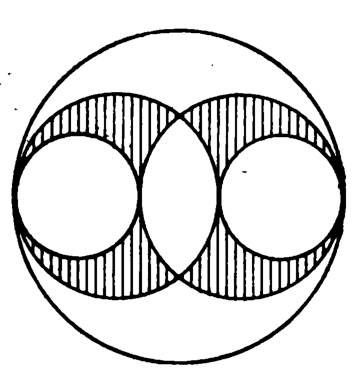
\includegraphics[width=0.6\linewidth]{pdf317-a.png}\end{center}

The rule given for the solution of this problem may be formulated thus:
\[
\text{(required surface)} = \sqrt{\sqrt{20}-2}\times(\text{diameter})^2.
\]

Another problem relates to the centre of gravity of a curve called the \emph{ōyen}, which is given as the locus described by a point on a small circle that rolls on another large circle, the point and the circle both rolling to the right along the respective circles in such a way that the point returns after a complete revolution to the starting position, where the two circles touch.''

Let the diameters of the large (the base) and the small (the rolling) circles be $d$ and $k$. Writing
\[
A=\frac{d}{k}+1,\quad B=A^2+2,\quad C=\sqrt{\left(1-\frac{1}{B}\right)+\frac{A}{4}}-\frac{A}{4},
\]
the areas of the circular segments with the sagittae
\[
s_1=\frac{1}{2}(C+1)\quad\text{and}\quad s_2=\frac{1}{2}(C-1),
\]
and the common chord $c=4s_1s_2$, will be found. We denote these areas by $a_1$ and $a_2$. Then the areas of the two portions of the curve cut by the line normal to the axis of symmetry through the centre of gravity will be
\[
A_1=(a_1B-c^3)(A+C)k^2,\quad A_2=(a_2B+c^3)(A+C)k^2,
\]
where $A$ is that part that lies to the side with the cusp.

3. Hagiwara wrote very much in the course of his long life. But he did not publish all; he only printed some of the results he had obtained. Most of the Japanese printed works concerning mathematics were of thin nature, the problems and the final formulae for their solution, expressed in the form of rules, being their sole contents. The detailed analysis of the problems considered was seldom given in published works. This usage had arizen certainly on ac-

\scanpage{0318}{printed page 304 (top left)}
\noindent count of the expense of printing, for the call for such books was exceedingly small and the wood-blocks were to be prepared by the authors themselves. The three books printed by Hagiwara are (1) the \emph{Sampō Hōyen-kan} of 1862, (2) the \emph{Sampō Yenri Shiron} of 1867 and (3) the \emph{Yenri San-yō} of 1878, which all relate to the circular theory of higher order. And in the decline of his life he attempted the publication of his last work, \emph{Reikan Sampō}, the results of his studies about the \emph{tenzan} problems. The publication was entrusted to the hand of C.~Kawakita several years ago, but it was not brought out during the life-time of the author, who died on the 28 th of November, 1909, at the advaneed age of 81. About the matter a comical event had occurred, of which I was a witness.\footnote{Hagiwara's \emph{Reikan Sampō} was published in 1910 by the kindness of K.~Nagasawa.}

After the Restoration of 1868 Hagiwara taught for a short time (1878---81) the normal school of Mayebashi. He also laboured some three years (1881---84) at the historical research work carried on by the Imperial University of Tokyo. Except for these few years he ever remained home at his native village. He was born as a farmer's son, lived as a farmer and died as such. If he had begun life in poverty, he was fortunate to make some fortune by his assiduity.

His writings are now preserved by his descendants in abundance. Resides the original analysis of his printed works, his tables used in folding or integration and his chronology of the Japanese mathematics may be of special value. In the following lines we have to say something about his results in published works. These may serve as specimens of the last development of the Japanese mathematics.

4. Here we give some of the problems considered by him.

Problem 6 of the \emph{Hōyen-kan}\footnote{These problems are described only after meanings, not being necessarily literal translations.} (abbreviated in the following as H.~K.). Given the diameters of the larger and smaller circles (the smaller being not greater than half of the greater), it is required to find the surface of the solid obtained by revolving the curve about its axis, which is the locus of a point on the smaller circle whose centre lies on the larger circle, when the smaller circle turns to the right along the larger circle and the point in the same direction along the smaller circle, at such a rate that it will return to its starting position after a complete revolution.

\scanpage{0319}{printed page 305}
Rule. The diameters of the greater and smaller circles being $d$ and $k$, we have
\[
\text{(surface)} = \left[40 - \left\{5 - \left(\frac{2k}{d}\right)^{2}\right\}^{2}\right] \times \frac{d^{2}\pi}{15}.
\]

Problem 22. H. K. A frustum of a pyramid with base a regular polygon is supposed to be deformed in such a way that the upper base being fixed the lower is turned in its plane just through a revolution. It is required to find the length of the line that corresponds to the lateral edge of the original frustum, being given the sides of the two bases and the altitude.

Problem 24. H. K. A frustum of an oblique circular cone with a generating line normal to the circular section is cut by a plane through the end of the said generating line at the larger base and normal to the plane of that generating line and the diameter of the other base drawn from its end, cutting from this diameter a sagitta of prescribed length. It is required to find the centre of gravity of the portion thus cut off.

Problem 26. H. K. To find the centre of gravity of the solid in problem 6.

Problem 28. H. K. To find the area of the portion of a hemi-sphere that will be illuminated by a lighted small sphere.

Problem 30. H. K. There is a spherical cap, which is supposed to be greater than a hemi-sphere, comprised between two planes inclined to each other. Suppose a spherical cap similar in form to the said one, also comprised between the two planes, is described touching that one. It is required to find the length of the curve described by the centre of the base of the second spherical cap.

Rule. Let $d$ be the diameter of the central sphere, $k$ that of the smallest sphere described touching it, and let $s$ be the sagitta of the central spherical cap. Then finding the perimeter of the ellipse, the squares of whose major and minor diameters are
\[
\left\{\frac{1}{2}\left(\frac{d}{k}+1\right)\right\}^{2} - \left[\left(\frac{s}{d}-0{\cdot}5\right)\left(\frac{d}{k}-1\right)\right]^{2} \quad\text{and}\quad \frac{d}{k},
\]
its product with $d + k$ will be the required length.

Problem 31. H. K. Three spheres $A$, $B$, $C$ are touching externally two by two. The sphere $B$ turns along a great circle of the sphere $A$ to the right, while $C$ turns to the left always keeping contact with the two other spheres, at such a rate that the two moving spheres will come back to the original position after a complete revolution.

\scanpage{0320}{printed page 306}
\noindent Then the locus of $C$ will divide the surface of $A$ into two portions, of which the greater is required to be evaluated in terms of the three diameters.

Rule.
\[
(\text{Area}) = \left\{\frac{BC}{(A+B)(A+C)}+0{\cdot}5\right\}A^2\pi.
\]

Problem 32. H. K. A sphere touches a right elliptic cone and the plane that is drawn through its vertex normal to its axis. When the sphere turns round always keeping these contacts, it will describe a locus on the plane, which is a closed curve. It is required to find its area in terms of the diameter $d$ of the sphere, the major and minor diameters $a$ and $b$ of a right section of the cone and $h$ the altitude of the section.

Rule. If we write
\[
t=\frac{(a^2-b^2)^2}{a^2(a^2+4h^2)},\quad k=\frac{4h^2(a^2-b^2)}{a^2(a^2\text{}+4h^2)},\quad l=4\left(1-\frac{b^2}{a^2}\right)\frac{a^2+2h^2}{a^2+4h^2},\quad A_r=k+rl;
\]
\begin{align*}
D_0&=\frac{b\sqrt{a^2+4h^2}}{a^2},\quad D_1=\frac{1}{2^2}kD_0,\quad D_2=\frac{3}{4^2}A_1D_1,\\
D_3&=\frac{5}{6^2}\left(A_2D_2-\frac{1.3}{2}tD_1\right),\quad D_4=\frac{7}{8^2}\left(A_3D_3-\frac{2.5}{3}tD_2\right),\\
D_5&=\frac{9}{10^2}\left(A_4D_4-\frac{3.7}{4}tD_3\right),\ldots,
\end{align*}
\noindent the required area will be given by
\[
\left\{1+\frac{a^2}{2h^2}\left(\frac{b}{a}+D_0+D_1+D_2+D_3+\cdots\right)\right\}d^2\times\frac{\pi}{4}.
\]

\begin{center}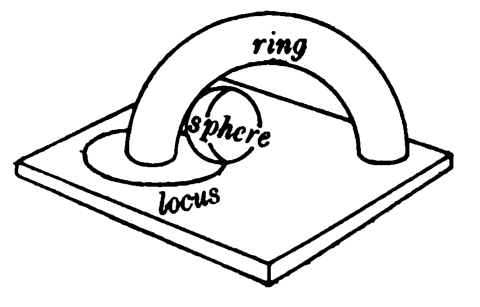
\includegraphics[width=0.6\linewidth]{pdf320-a.png}\end{center}

Problem 33. H. K. The half of an anchor-ring stands on a plane as shown in the figure, and a sphere that touches both the ring and the plane (the diameter $d$ of the sphere being at most equal to the difference of those of the right section of the ring and the axial section normal to it, which we denote by $k$ and $l$), turns round the ring describing a locus on the plane. It is required to find the area of this curve.

Rule. If we write
\[
p=\frac{(k+d)(l+d)}{k^2+2kd},\qquad q=\frac{l+d}{k+d},
\]
\noindent and
\[
D_0=\frac{\pi}{4}p(l+d)\sqrt{k^2+2kd},\quad D_1=(p-q)D_0,\quad D_2=\frac{3.5}{2.4}pD_1,
\]

\scanpage{0321}{printed page 307}
\[
D_3 = \frac{5.11}{3.5}\text{}\,p\Bigl(D_2 - \frac{1.3}{2.4}\text{}\,qD_1\Bigr), \qquad
D_4 = \frac{7.9}{4\;6}\text{}\,p\Bigl(D_3 - \frac{2.4}{3.4}\,qD_2\Bigr),
\]
\[
D_5 = \frac{9.11}{5.7}\,p\Bigl(D_4 - \frac{3.5}{4.6}\,qD_3\Bigr), \ldots,
\]
the required area will be given by $D_0 + D_1 + D_2 + \cdots$

Problem 34. H. K. Let there be two circles $A$ and $B$, of which $A$ is the greater, touching each other with a common tangent between them. The circle $A$ rolls along the line to the left, while the circle $B$ turns to the right keeping contact with $A$, and the spot on the circle $B$ which is originally coincident with the point of contact of the base line, rolls along the circle $B$ to the right, describing a locus as shown in the figure in complete revolutions. Given the diameters of the circles $A$ and $B$ and the length of $MN = p$, it is required to find the area of the curve.

\begin{center}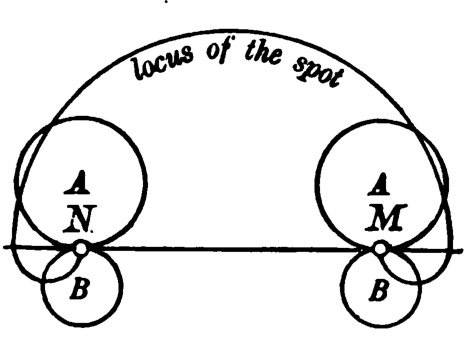
\includegraphics[width=0.6\linewidth]{pdf321-a.png}\end{center}

Rule.\quad Area $= \Bigl\{2B^2 + (A + B)^2\Bigr\}\,\frac{\pi}{4} + \frac{A}{2} \times p$.

Problem 35. H. K. This is the same as problem 33, only that the whole ring is taken instead of the half of it in the previous problem.

Problem 8 of the \emph{Sampō Yenri Shiron} (which we abbreviate S.Y.S.).\footnote{This work was a revision of the solutions published by the author's predecessors concerning the problems in the circular theory of higher order.} When a circular cylinder is pierced by an elliptic cylinder going obliquely as shown in the figure, the axes of the two being supposed to be at right angles with one another, it is required to find the volume of the pierced portion, given the diameter $d$ of the circular cylinder and the major and minor diameters $a$ and $b$ of the base of the elliptic cylinder and also the lengths indicated $s_1$ and $s_2$ in the figure, which are drawn normal to the generating lines in reference.

\begin{center}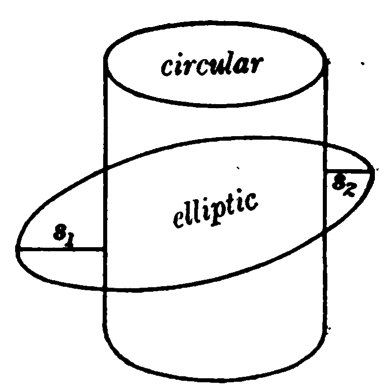
\includegraphics[width=0.6\linewidth]{pdf321-b.png}\end{center}

This problem was first given in Saitō Gigi's \emph{Yenri-kan} of 1834, but Hagiwara revised its solution as being incorrect.

\scanpage{0322}{printed page 308 (top left)}
Problem 9. S. Y. S. A circular cone, the diameter of whose base is $d$, is bended as in the figure, so that the axis $h$ becomes an arc of a circle of diameter $d'$. It is required to find the lengths of the curves corresponding to the generating lines in the plane of the circle of bending.

\begin{center}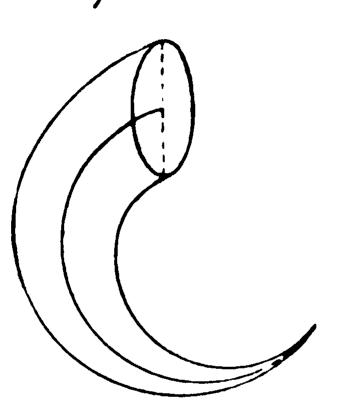
\includegraphics[width=0.6\linewidth]{pdf322-a.png}\end{center}

This was first published in Kobayashi's \emph{Sampō Koren} of 1836, in the solution of which was employed the \emph{tetsu-jutsu} expansion three times. Afterwards it was also solved in Kuwamoto's \emph{Sen-yen Kattsū} of 1855. But both solutions had not been very simple and so Hagiwara solved it anew with the double application of the expansion process.

\begin{center}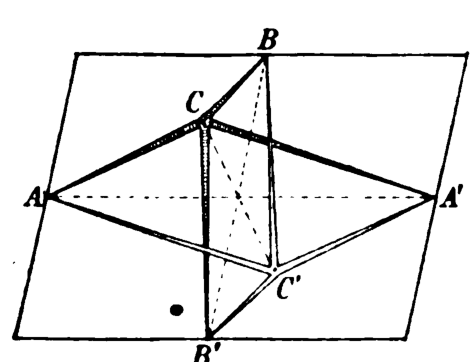
\includegraphics[width=0.6\linewidth]{pdf322-b.png}\end{center}

Problem 10. S. Y. S. The area of a \emph{choku-bishi} (which is a kind of skew surface) is required in terms of the three axes $AA' = a$,\quad $BB' = b$,\quad $CC' = c$. The \emph{choku-bishi} is such a surface or figure composed of surfaces that the sections parallel to any two of the axes are all rhombi.

The solution of this problem given in the \emph{Sampō Koren} being not convenient and that in Saitō's \emph{Yenri Shinshin} being incorrect, Hagiwara obtained a revised solution.

Problem 31. S.Y.S. The surface area of the portion of an elliptic cone intercepted by a circular cylinder, the axes of the two intersecting at right angles, is required.

Hagiwara's solution was a revision of that in Murayama's \emph{Tsūki Sampō}.

\begin{center}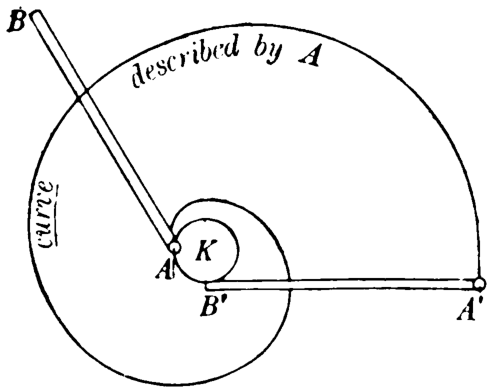
\includegraphics[width=0.6\linewidth]{pdf322-c.png}\end{center}

Problem 32. S. Y. S. A rod $AB = p$, which is tangent to a circle $K$ at its one end $A$, turns round the circumference without sliding, when its end $A$ describes a curve as shown in the figure, terminating at a point $A'$, when the rod assumes the position of $A'B'$, with another end $B$ now touching the circle. It is required to find the length of the curve and the area bounded by it, the circle, and the final position of the rod.

Rule. If we write $s =$ length and $a =$ area, we have
\[
s = \frac{p^2}{K}, \quad \text{and} \quad a = s\times\frac{p}{3} - \frac{(p-K\pi)^3}{3K}, \quad \text{or} \quad a = s\times\frac{p}{3},
\]

\scanpage{0323}{printed page 309}
\noindent where the two formulae of the area are applicable when $p - K\pi$ is or is not positive.

This problem was previously considered in the \emph{Tsūki Sampō}, but the rule given there was applicable only to the case where the rod did not revolve round the circle more than a complete revolution. Hagiwara therefore revised it so as to become generally applicable.

Problem 34. S. Y. S. It is required to find the area of the surface resulting from the revolution of a cycloid with its greatest ordinate as axis.

Rule. Area $= \left(2 - \dfrac{2}{3 \times \frac{\pi}{4}}\right)k^2$, where $k$ is the length of the base of the cycloid.

This was a revision of the solution given in the \emph{Tsui-yen Hatsumō}.

Problem 4 of \emph{Yenri San-yō} (Y. S.). Two congruent circular cones of equal altitudes are intersecting at right angles as in the figure. It is required to balance it so that the axis of one of them should be horizontal.

\begin{center}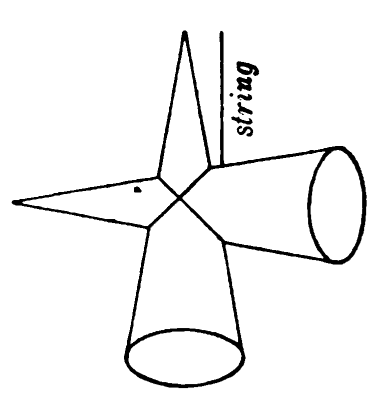
\includegraphics[width=0.3\linewidth]{pdf323-a.png}\quad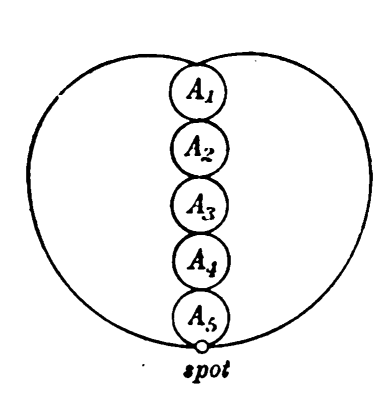
\includegraphics[width=0.3\linewidth]{pdf323-b.png}\end{center}

Problem 14. Y. S. There are described a number ($n$) of equal circles (diameter $d$) with their centres on a straight line and touching successively. Let there be a spot on the circumference of the last circle on this said line. If then the second circle revolves round the first, the third round the second, and so on, the directions of the revolutions being all the same, the spot will describe a locus, whose form is as shown in the above figure, returning to its starting point after a complete revolution. It is required to find the area of the oval.

Rule. Area $= (2n - 1)n \times \frac{\pi}{4} \times d^2$.

Problem 15. Let there be described an even number $2n$ of circles all touching at a common point $T$, such that the 1st, 3rd, \dots\ circles lie to one side of $T$, while the remaining 2nd, 4th, \dots\ lie to the other side of it, forming two series of circles consisting of equal numbers, arranged in order of size, the 1st and 2nd being the greatest of the respective series. Let $K$ be the centre of the $2n$th circle, and let there be a spot at $K$ which is assumed as belonging to the

\scanpage{0324}{printed page 310 (top left)}
\noindent circumference of the circle described with $T$ as centre and passing through the point. Now the 2nd circle turns round the 1st circle, the 3rd round the 2nd, and so forth, all to the right. The circle $T$ is carried with its centre on the $2n$th circle, and the point or spot $K$ is carried on the circle $T$. The nature of the turnings are so conceived that the whole figure will assume its original form after a complete revolution. The locus which $K$ describes is obviously a closed curve and so also that of $T$. It is required to find the area of the annulus formed by these two loci.

\begin{center}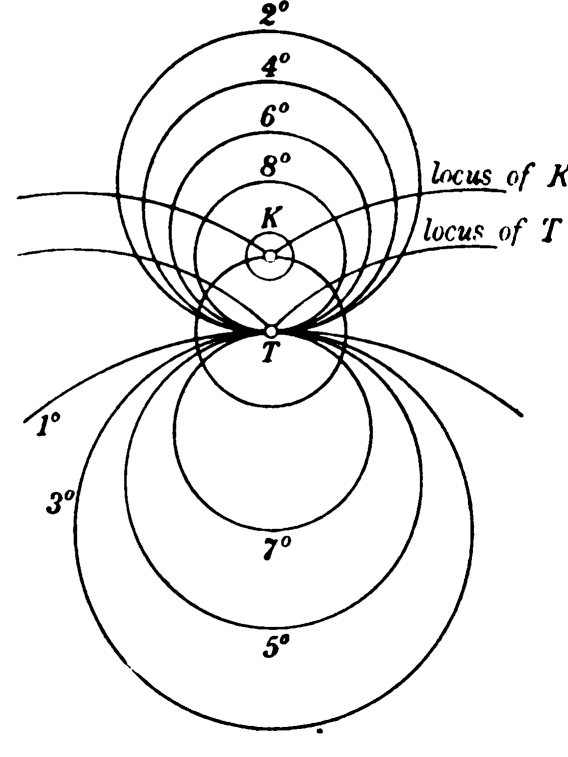
\includegraphics[width=0.6\linewidth]{pdf324-a.png}\end{center}

Rule. If the diameter of the circle $T$ be $d$, the required area will be $d^2\times\frac{\pi}{4}\times(2n+1)$.

Problem 20. Y. S. It is required to find the volume of a figure that is formed by four equal circular cones as shown in the figure, in terms of the altitude and diameter of the cones and the length and breadth of the figure.

\begin{center}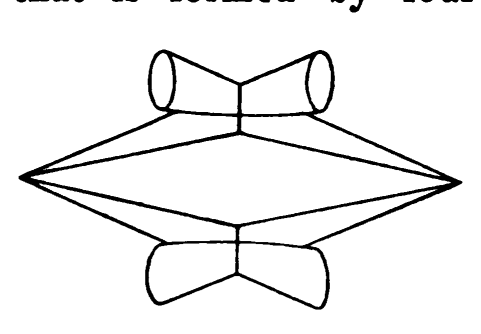
\includegraphics[width=0.6\linewidth]{pdf324-b.png}\end{center}

There are also problems requiring the volumes and lateral surfaces of the figures composed of a number of equal cones in a similar way as in this problem.

Problem 25. Y. S. There is a figure composed by intersecting a circular cylinder obliquely with an ellipsoid of revolution such that the latter internally touches a generating line of the former. If this solid be suspended in equilibrium by a string coinciding with the generating line opposite the said one, how long will be the altitude of the cylinder? Here the major and minor diameters of the ellipsoid, the former being the axis of revolution, the longest sagitta drawn normal to the line of suspension\footnote{We mean by this phrase the greatest normal distance of a point on the ellipsoid from the line of reference at the opposite side of the cylinder.} and the diameter of the cylinder are assumed to be known.

Problem 30. Y. S. An ellipsoid of revolution with the major diameter as axis, from which a hole is pierced by a circular cylinder that touches one end of this diameter, is placed on a plane board.

\scanpage{0325}{printed page 311}
\noindent Cut it by the vertical plane through its point of contact with the board and normal to the vertical plane containing the axis. Given the two diameters of the ellipsoid and the diameter of the cylinder, it is required to find the volume of the cut off portion.

5. The solutions of some of the problems considered by Hagiwara will be given in the next chapters. In the rules of his solutions he sometimes used the logarithmic series, but this was borrowed by him from the Occidental science through the suggestion of his friend Okamoto Norifumi.

It is said that there was no one, to the greatest satisfaction of Hagiwara's pride, in the whole Empire, who could verify the results of all the questions in the \emph{Yenri San-yō}, with the single exception of Ōmura Isshū, who was able to solve some of the problems. Ōmura was versed in something of the European mathematics, although his knowledge in this domain was of a most limited kind.

Hagiwara was a person rarely convinced to admit the superiority of others in their studies. But he could not help admiring the talents of this Ōmura, who was his senior by a few years. Hōdōji Wajūrō, Suzuki Yen, Takaku Kenjirō, Iwata Sempei (better known as Iwata Kōsan, Kōsan being his literary name), and others were among those for whom he had shown his respect. He had a good opinion of Sonobe Keizō, mathematician of Takuma's\unclear{Takuma's / Takumá's / Takumā's} school, who perhaps still lives.

Among Hagiwara's unpublished works we may mention the tables constructed or revised by him for the purpose of folding or integration. Of these tables we hope to have a good occasion for carrying out our studies. The rest of Hagiwara's writings are, we hope, full of deep interest to constitute the theme of our further studies.

\begin{center}
CHAPTER 45.\\[1mm]
HAGIWARA'S FORMULA FOR THE AREA OF THE CURVE DESCRIBED BY A SPHERE ROLLING ROUND AN ANCHOR-RING STANDING ON A PLANE.
\end{center}
\phantomsection\addcontentsline{toc}{subsection}{Chapter 45. Hagiwara's Formula for the Area of the Curve Described by a Sphere Rolling Round an Anchor-Ring Standing on a Plane}

Hagiwara Teisuke's \emph{Sampō Hōyen-kan}, printed in 1862, contains a problem which runs as follows: ``There is an anchor-ring standing normally on a flat stand. A sphere that touches the ring at its base rolls round it until returning to the first position after a whole circuit. The path described by the sphere on the plane is of a

\scanpage{0326}{printed page 312}
special form. Given the diameter of the ring, the diameter of its section, and the diameter of the sphere (equal to that of the ring when greatest), it is required to find the area of the locus.''

\begin{center}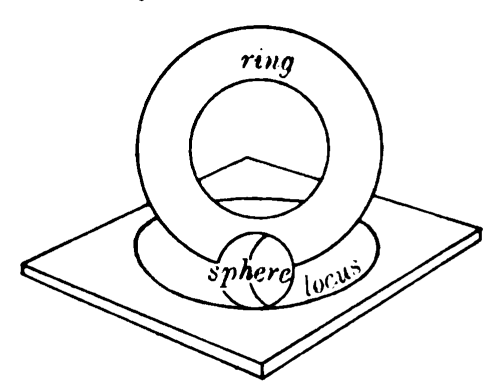
\includegraphics[width=0.6\linewidth]{pdf326-a.png}\end{center}

Let the diameter of the ring be $a$, that of the sphere $b$, and that of the section of the ring $c$. Then Hagiwara's rule for solution may be expressed by
\[
(\text{area}) = ab\pi(D_0 - D_1 - D_2 - D_3 - \cdots),
\]
where writing $k = \dfrac{a}{b+c}$ and $t = \dfrac{b}{a}$, and
\[
A = \frac{1}{\sqrt{k}}, \quad B = \frac{3}{1\,.\,2}Ak, \quad C = \frac{1\,.\,5}{3\,.\,4}Bk, \quad D = \frac{3\,.\,7}{5\,.\,6}Ck, \quad E = \frac{5\,.\,9}{7\,.\,8}Dk, \ldots;
\]
\[
\alpha = \frac{1}{4}t, \quad \beta = \frac{3}{6}\alpha t, \quad \gamma = \frac{5}{8}\beta t, \quad \delta = \frac{7}{10}\gamma t, \ldots;
\]
the quantities $D_0$ and $D_1$, $D_2$, .\,., are of the forms
\begin{align*}
&D_0 = A, \quad D_1 = \alpha\Bigl(B + \tfrac{1}{2}A\Bigr), \quad D_2 = \beta\Bigl[C - \tfrac{1}{2}\Bigl(B - \tfrac{1}{4}A\Bigr)\Bigr],\\
&D_3 = \gamma\Bigl[D - \tfrac{1}{2}\Bigl\{C + \tfrac{1}{4}\Bigl(B - \tfrac{3}{6}A\Bigr)\Bigr\}\Bigr],\\
&D_4 = \delta\Bigl[E - \tfrac{1}{2}\Bigl\{D + \tfrac{1}{4}\,\Bigl|\overline{C + \tfrac{3}{6}\Bigl(B - \tfrac{5}{8}A\Bigr)}\Bigr\}\Bigr], \ldots
\end{align*}

In Hagiwara's work this rule was published without any explanation. We propose here to supply the analysis of the problem as tried by Ōmura Isshū in one of his manuscripts.

Ōmura first gives the figures as reproduced in this place.

\begin{center}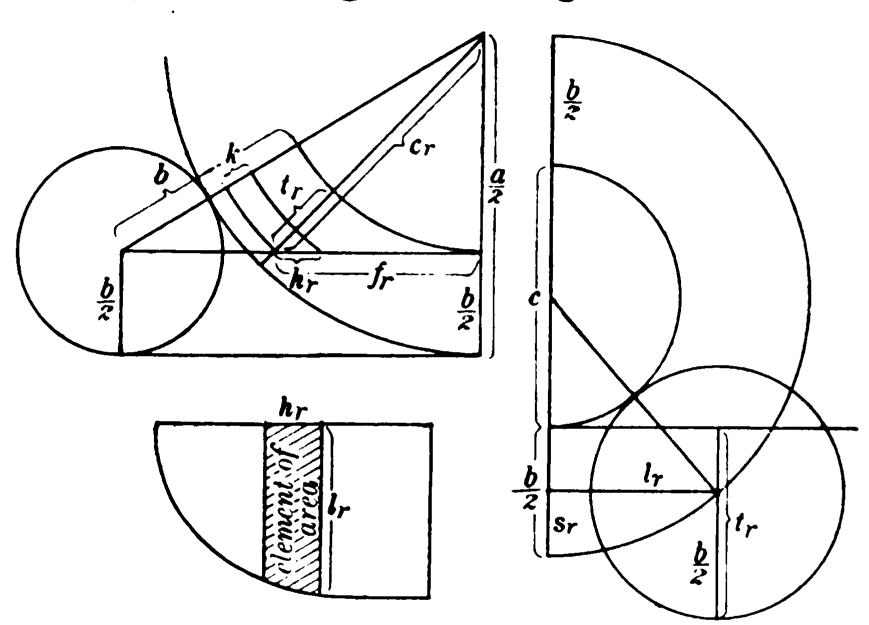
\includegraphics[width=0.6\linewidth]{pdf326-b.png}\end{center}

Here the construction of the figures is not explained, and there are some points that are not easily comprehensible, but we shall only follow the analysis attempted. The nature of the figures may be revealed from the expressions of the various lengths. Thus $n$ being the number of divisions we have
\[
k = \frac{b}{n}; \quad t_r = b \times \frac{r}{n} = bi,\ \text{say}; \quad s_r = b - t_r = (1 - i)b;
\]
\[
l_r^2 = (b + c)s_r - s_r^2 = (1 - i)b(b + c)\{1 - \varrho(1 - i)\},
\]

\scanpage{0327}{printed page 313}
\noindent where $\varrho = b/(b + c)$, or expanded
\begin{multline*}
l_r = \sqrt{1 - i}\,\sqrt{b}\,\sqrt{b + c}\,\Bigl\{1 - \tfrac{1}{2}(1 - i)\,\varrho - \tfrac{1}{8}(1 - i)^2\varrho^2 - \tfrac{3}{48}(1 - i)^3\varrho^3\\
{} - \tfrac{15}{384}(1 - i)^4\varrho^4 - \cdots\Bigr\};
\end{multline*}
\[
c_r = t_r + \frac{a + b}{2} = ib + \frac{a - b}{2};
\]
\[
f_r^2 = c_r^2 - \left(\frac{a - b}{2}\right)^2 = i^2b^2 - ib^2 + iab = iab\{1 - \Phi(1 - i)\},
\]
where $\Phi = b/a$, and from this we have
\begin{multline*}
\frac{1}{f_r} = \frac{1}{\sqrt{abi}}\Bigl\{1 + \tfrac{1}{2}\Phi(1 - i) + \tfrac{3}{8}\Phi^2(1 - i)^2 + \tfrac{15}{48}\Phi^3(1 - i)^3\\
{} + \tfrac{105}{384}\Phi^4(1 - i)^4 + \cdots\Bigr\};
\end{multline*}
\[
\frac{h_r}{k} = \frac{c_r}{f_p} = \frac{1}{f_r}\,a\Bigl\{\tfrac{1}{2} + \tfrac{1}{2}\Phi - \Phi(1 - i)\Bigr\},
\]
\begin{multline*}
\therefore\ \frac{h_r\sqrt{abi}}{k} = a\Bigl\{\tfrac{1}{2} - \tfrac{3}{4}\Phi(1 - i) - \tfrac{5}{16}\Phi^2(1 - i)^2 - \tfrac{21}{96}\Phi^3(1 - i)^3\\
\shoveright{{} - \tfrac{135}{2.384}\Phi^4(1 - i)^4 - \cdots\Bigr\}}\\
{} + a\Phi\Bigl\{\tfrac{1}{2} + \tfrac{1}{4}\Phi(1 - i) + \tfrac{3}{16}\Phi^2(1 - i)^2 + \tfrac{15}{96}\Phi^3(1 - i)^3\\
{} + \tfrac{105}{2.384}\Phi^4(1 - i)^4 + \cdots\Bigr\};
\end{multline*}
and writing the element of area $= A_r = h_r\,l_r$, we have
\[
\begin{array}{@{}l@{\;}l@{\;}l@{\;}l@{\;}l@{}}
\multicolumn{5}{c}{\dfrac{A_r}{k\sqrt{a\,(b + c)}}}\\[4mm]
= \dfrac{\sqrt{1 - i}}{2\sqrt{i}}
 & {} - \dfrac{3\sqrt{1 - i}\,(1 - i)}{4\sqrt{i}}\,\Phi
 & {} - \dfrac{5\sqrt{1 - i}\,(1 - i)^2}{16\sqrt{i}}\,\Phi^2
 & {} - \dfrac{21\sqrt{1 - i}\,(1 - i)^3}{96\sqrt{i}}\,\Phi^3
 & {} - \cdots\\[4mm]
+ \dfrac{\varrho}{2}\biggl(
 & {} - \dfrac{\sqrt{1 - i}\,(1 - i)}{2\sqrt{i}}
 & {} + \dfrac{3\sqrt{1 - i}\,(1 - i)^2}{4\sqrt{i}}\,\Phi
 & {} + \dfrac{5\sqrt{1 - i}\,(1 - i)^3}{16\sqrt{i}}\,\Phi^2
 & {} + \cdots\biggr)\\[4mm]
+ \dfrac{\varrho^2}{8}\biggl(
 &
 & {} - \dfrac{\sqrt{1 - i}\,(1 - i)^2}{2\sqrt{i}}
 & {} + \dfrac{3\sqrt{1 - i}\,(1 - i)^3}{4\sqrt{i}}\,\Phi
 & {} + \cdots\biggr)\\[4mm]
+ \dfrac{3\varrho^3}{48}\biggl(
 &
 &
 & {} - \dfrac{\sqrt{1 - i}\,(1 - i)^3}{2\sqrt{i}}
 & {} + \cdots\biggr)\\[4mm]
+ & \multicolumn{4}{l}{\dotfill}
\end{array}
\]

\scanpage{0328}{printed page 314 (top left)}
\[
\begin{array}{@{}r@{\,}l@{\;}l@{\;}l@{\;}l@{}}
+ & \dfrac{\sqrt{1-i}}{2\sqrt{i}}\,\varPhi
  & {}+\dfrac{\sqrt{1-i}\,(1-i)}{4\sqrt{i}}\,\varPhi^{2}
  & {}+\dfrac{3\sqrt{1-i}\,(1-i)^{2}}{16\sqrt{i}}
  & {}+\cdots\\[4mm]
+ & \dfrac{\varrho}{2}\Biggl(
  & {}-\dfrac{\sqrt{1-i}\,(1-i)}{4\sqrt{i}}\,\varPhi
  & {}-\dfrac{\sqrt{1-i}\,(1-i)^{2}}{4\sqrt{i}}\,\varPhi^{2}
  & {}-\cdots\Biggr)\\[4mm]
+ & \dfrac{\varrho^{2}}{8}\Biggl(
  &
  & {}-\dfrac{\sqrt{1-i}\,(1-i)^{2}}{2\sqrt{i}}\,\varPhi
  & {}-\cdots\Biggr)\\[4mm]
+ & \multicolumn{4}{l}{.\quad.\quad.\quad.\quad.\quad.\quad.\quad.\quad.\quad.\quad.\quad.\quad.\quad.\quad.\quad.\quad.\quad.\quad.}
\end{array}
\]

If we fold this expression, or sum up for $i=\frac{1}{n},\frac{2}{n},\cdots,\frac{n}{n}$ and go to the limit $n=\infty$, we shall have
\[
\begin{array}{@{}l@{}}
\begin{array}{@{}r@{\,}l@{\;}l@{\;}l@{\;}l@{\;}l@{}}
\dfrac{\text{(area)}}{\pi b\sqrt{a}\cdot\sqrt{b+c}}={}
  & \dfrac{2}{2}
  & {}-\dfrac{3\cdot3\varPhi}{2.4}
  & {}-\dfrac{5.15\varPhi^{2}}{2.6.16}
  & {}-\dfrac{21.105\varPhi^{3}}{2.8.6.96}
  & {}-\cdots\\[3mm]
+ & \dfrac{\varrho}{2}\biggl(
  & {}-\dfrac{3}{2.2}
  & {}+\dfrac{3.15\varPhi}{2.6.4}\text{}
  & {}+\dfrac{5.105\varPhi^{2}}{2.8.6.16}
  & {}+\cdots\biggr)\\[3mm]
+ & \dfrac{\varrho^{2}}{8}\biggl(
  &
  & {}-\dfrac{15}{2.6.2}
  & {}+\dfrac{3.105\varPhi}{2.8.6.4}
  & {}+\cdots\biggr)\\[3mm]
+ & \dfrac{3\varrho^{3}}{48}\biggl(
  &
  &
  & {}-\dfrac{105}{2.8.6.2}
  & {}+\cdots\biggr)+\cdots
\end{array}\\[3mm]
\qquad\quad
\begin{array}{@{}r@{\,}l@{\;}l@{\;}l@{\;}l@{\;}l@{}}
+ & \dfrac{2\varPhi}{2}
  & {}+\dfrac{3\varPhi^{2}}{4}
  & {}+\dfrac{3.15\varPhi^{3}}{2.6.16}
  & {}+\dfrac{15.105\varPhi^{4}}{2.6.8.96}
  & {}+\cdots\\[3mm]
+ & \dfrac{\varrho}{2}\biggl(
  & {}-\dfrac{3\varPhi}{2.2}
  & {}-\dfrac{15\varPhi^{2}}{2.6.4}
  & {}-\dfrac{3.105\varPhi^{3}}{2.8.6.16}
  & {}-\cdots\biggr)\\[3mm]
+ & \dfrac{\varrho^{2}}{8}\biggl(
  &
  & {}-\dfrac{15\varPhi}{2.6.2}
  & {}-\dfrac{105\varPhi^{2}}{2.8.6.4}
  & {}-\cdots\biggr)\\[3mm]
+ & \dfrac{3\varrho^{3}}{48}\biggl(
  &
  &
  & {}-\dfrac{105\varPhi}{2.8.6.2}
  & {}-\cdots\biggr)+\cdots
\end{array}\\[3mm]
\begin{array}{@{}r@{\,}l@{\;}l@{\;}l@{\;}l@{\;}l@{\;}l@{}}
={} & \dfrac{2}{2}
  & {}-\dfrac{\varPhi}{8}
  & {}-\dfrac{3\varPhi^{2}}{2.6.16}
  & {}-\dfrac{3.15\varPhi^{3}}{2.8.6.96}
  & {}-\dfrac{15.105\varPhi^{4}}{2.10.8.6.2.384}
  & {}-\cdots\\[3mm]
  &
  & {}-\dfrac{3\varrho}{8}
  & {}+\dfrac{9\varPhi\varrho}{2.48}
  & {}+\dfrac{45\varPhi^{2}\varrho}{8.384}
  & {}+\dfrac{945\varPhi^{3}\varrho}{48.3840}
  & {}+\cdots\\[3mm]
  &
  &
  & {}-\dfrac{15\varrho^{2}}{192}
  & {}+\dfrac{75\varPhi\varrho^{2}}{8.384}
  & {}+\dfrac{105.5\varPhi^{2}\varrho^{2}}{48.3840}
  & {}+\cdots\\[3mm]
  &
  &
  &
  & {}-\dfrac{105.3\varrho^{3}}{48.192}
  & {}+\dfrac{105.21\varPhi\varrho^{3}}{48.3840}
  & {}+\cdots\\[3mm]
  &
  &
  &
  &
  & {}-\dfrac{945.15\varrho^{4}}{5.164^{2}}\text{}
  & {}+\cdots\\[2mm]
  &
  &
  &
  &
  & \multicolumn{2}{l}{.\quad.\quad.\quad.\quad.\quad.\quad.}
\end{array}
\end{array}
\]

Hagiwara's rule follows from this double series.

\scanpage{0329}{printed page 315 (top right)}
\begin{center}
CHAPTER 46.\\[1mm]
THE SKEW SURFACE.
\end{center}
\phantomsection\addcontentsline{toc}{subsection}{Chapter 46. The Skew Surface}

1. Let $ABCD$ be a gauche quadrilateral. Divide the opposite sides $AB$ and $CD$ into an equal number of equal parts and join the corresponding points of division by straight lines. With the other pair of opposite sides $AD$ and $BC$, the same construction is performed. The result is a kind of net. If the numbers of divisions of the two pairs are increased without limit, we get a skew surface. The calculations of some figures connected with such a surface were attempted by the Japanese mathematicians of the 19th century.

The first place we meet with the question about this surface is Kobayashi's \emph{Sampō Koren}, printed in 1836. It is the same problem of the \emph{choku-bishi} as subsequently studied by Hagiwara. If we take three mutually rectangular axes intersecting in their middle points and form a rectangle with two of the axes as a pair of medians, there will be formed eight gauche quadrilaterals with the segments of the sides of the rectangle and the joining lines of the end-points of the axes, of which those that are coplanar with the rectangle are excluded. The figure enclosed by the skew surfaces with these gauche quadrilaterals as bases is the so-called \emph{choku-bishi}.

Kobayashi's result of the problem of finding the whole surface of the figure was given as suspended before a temple at Uyeda in the province of Shinano.

In Saitō's \emph{Yenri Shinshin} of 1840 the problem was considered of finding the lateral surface of a figure which is the half of a \emph{choku-bishi}.

Fujioka Yūtei also considered the surface in his \emph{Sampō Yenri-tsū} of 1845. There are still other printed works, where we find the problems relating to the skew surface. But all these publications only contain the results of calculations, there being none in which the analysis is considered at the same time. We have therefore no knowledge of the treatment followed by Kobayashi, and other earlier writers. We have consequently to describe the ways of procedure tried by Hōdōji Wajūrō and Hagiwara Teisuke.

2. There is a manuscript written by Hōdōji entitled ``The Analysis of the 12th Problem of the \emph{Sampō Koren}''. We give the results of the book. In the first place he considers as follows: Let $ABCD$ be the skew surface which is to be quadrated. Make a con-

\scanpage{0330}{printed page 316}
struction as shown in the figure, where $DCB'A'$ is a rectangle, $AA'$
and $BB'$ normal to its plane, $PQ \parallel P_1Q_1 \parallel AB$, $PP' \parallel P_1P_1' \parallel AA'$,
\begin{center}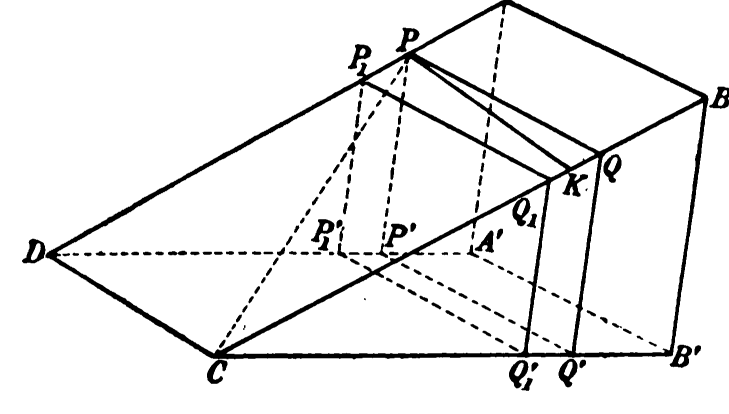
\includegraphics[width=0.6\linewidth]{pdf330-a.png}\end{center}
$QQ' \parallel Q_1Q_1' \parallel BB'$, $P'Q' \parallel P_1'Q_1' \parallel A'B'$. Suppose $PQQ'P'$, $P_1Q_1Q_1'P_1'$ are two consecutive planes
among the parallel planes drawn
at equal intervals dividing the
skew surface into $n$ parts. Then
we may write $Q'Q_1' = \frac{1}{n} \cdot B'C$
and $Q'C = \frac{r}{n} \cdot B'C$. Let $PC$
be joined and $PK$ be drawn from $P$ at right angles to $BC$. We shall
first take $PK.QQ_1$ as the element of area $(A_r)$. We have thus\footnote{The derivation of the expression for $KC$ is not given.}
\[
PC^2 = CQ'^2 + P'Q'^2 + PP'^2, \quad KC = \frac{r}{n}\,\frac{1}{BC}\,(B'C^2 + AA'.BB'),
\]
\[
\therefore PK^2 = PC^2 - KC^2 = CD^2 + (AA' - BB')^2 CB'^2 \cdot \frac{1}{BC^2} \cdot \frac{r^2}{n^2},
\]
which we write $= CD^2 \left\{1 + \frac{r^2}{n^2}\alpha\right\}$, say. And it follows
\[
\begin{aligned}
A_r = PK.QQ_1 = BC.CD \cdot \frac{1}{n}\biggl\{1 + \frac{1}{2}\alpha\left(\frac{r}{n}\right)^2 - \frac{1}{8}\alpha^2\left(\frac{r}{n}\right)^4 + \frac{3}{48}\alpha^3\left(\frac{r}{n}\right)^6 &\\
- \frac{15}{384}\alpha^4\left(\frac{r}{n}\right)^8 + \cdots\biggr\}&,
\end{aligned}
\]
and the operatiou of folding, i.\ e., integration by terms, gives
\[
\begin{aligned}
\text{(area)} &= BC.CD\left\{1 + \frac{1}{3\,.\,2}\alpha - \frac{1}{5\,.\,8}\alpha^2 + \frac{3}{7\,.\,48}\alpha^3 - \frac{15}{9\,.\,384}\alpha^4 + \cdots\right\}\\
&= BC.CD\left\{1 + \frac{1}{2\,.\,3}\alpha - \frac{1\,.\,3}{4\,.\,5}\alpha D_1 + \frac{3\,.\,5}{6\,.\,7}\alpha D_2 - \frac{5\,.\,7}{8\,.\,9}\alpha D_3 + \cdots\right\},
\end{aligned}
\]
where $D_1$, $D_2, \ldots$ denote as usual the successive differences.

But if the above procedure be legitimate, it must also be legitimate to draw the perpendicular $QK'$ from $Q$ to $AD$ and take $QK'.PP_1$
as the element of area. In this case calculation\footnote{Which is given by Hōdōji as in the previous case.} will lead to the
formula:
\[
\text{(area)} = AD.CD\left\{1 + \frac{1}{2\,.\,3}\alpha' - \frac{1\,.\,3}{4\,.\,5}\alpha' D_1 + \frac{3\,.\,5}{6\,.\,7}\alpha' D_2 - \frac{5\,.\,7}{8\,.\,9}\alpha' D_3 + \cdots\right\},
\]
where we have $\alpha' = (AA' - BB')B'C^2/CD^2.AD^2$ instead of the former
$\alpha = (AA' - BB')^2 B'C^2/CD^2.BC^2$.

If we give some numerical values to the length considered in
the problem, the above two formulae will be seen to give somewhat

\scanpage{0331}{printed page 317}
\noindent different values to the area in question,\footnote{Neither the numerical calculations nor the results are given, except the conclusion.} which is the testimonial of the illegitimacy of both the formulae.

\begin{center}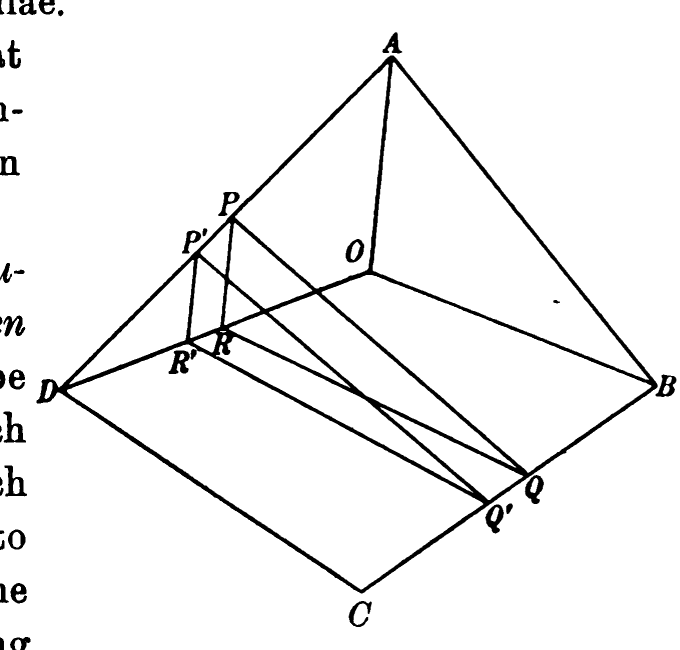
\includegraphics[width=0.6\linewidth]{pdf331-a.png}\end{center}

3. Hōdōji thus concludes that the above way of treatment is incorrect but he proceeds thereupon to make further considerations.

One eighth part of the \emph{chokubishi} considered in the \emph{Sampō Koren} is of the form annexed and may be conceived as consisting of such elementary parts as $PQQ'P'$, which are cut off by planes parallel to $ABO$ drawn at equal intervals. One of these parts is treated according to the first of the two formulae obtained above. Here we have
\[
QQ' = \frac{1}{n}\cdot OD, \quad PR = \frac{r}{n}\,OA, \quad P'R' = \left(\frac{r}{n} - \frac{1}{n}\right) OA,
\]
\[
PQ^2 = OB^2 + \left(\frac{r}{n}\right)^2 OA^2 = OB^2\,.\,k,
\]
where we write
\[
t = \frac{OA^2}{OB^2}, \quad k = 1 + \left(\frac{r}{n}\right)^2 t;\ \text{and also}\ s = \frac{OA^2}{OD^2}.
\]

Then applying the said formula, whereby we write $2\,.\,OB = a$, $2\,.\,OD = b$, $2\,.\,OA = c$, and taking 4 times of $PQQ'P'$ as the element of area $(A_r)$, we have
\[
A_r = ab\,\frac{1}{n}\left\{\sqrt{k} + \frac{1}{3.2}\,\frac{s}{\sqrt{k}} - \frac{1}{5.8}\,\frac{s^2}{k\sqrt{k}} + \frac{3}{7\,.\,48}\,\frac{s^3}{k^2\sqrt{k}} - \frac{15}{9.384}\,\frac{s^4}{k^3\sqrt{k}} + \cdots\right\}.
\]

If we denote the successive terms within the brackets by $D_0$, $D_1$, $D_2, \ldots$ and expand $\sqrt{k}$, we get
\[
\begin{array}{@{}l@{\;}c@{\;}l@{}}
D_0 = & & \left\{\phantom{-}1 + \frac{1}{2}\,t\left(\frac{r}{n}\right)^{2} - \frac{1}{8}\,t^{2}\left(\frac{r}{n}\right)^{4} + \frac{3}{48}\,t^{3}\left(\frac{r}{n}\right)^{6} - \frac{15}{384}\,t^{4}\left(\frac{r}{n}\right)^{8} + \cdots\right\},\\[3mm]
D_1 = & \frac{s}{3\,.\,2} & \left\{\phantom{-}1 - \frac{1}{2}\,t\left(\frac{r}{n}\right)^{2} + \frac{3}{8}\,t^{2}\left(\frac{r}{n}\right)^{4} - \frac{15}{48}\,t^{3}\left(\frac{r}{n}\right)^{6} + \frac{105}{384}\,t^{4}\left(\frac{r}{n}\right)^{8} - \cdots\right\}.\\[3mm]
D_2 = & \frac{s^{2}}{5\,.\,8} & \left\{-1 + \frac{3}{2}\,t\left(\frac{r}{n}\right)^{2} - \frac{15}{8}\,t^{2}\left(\frac{r}{n}\right)^{4} + \frac{105}{48}\,t^{3}\left(\frac{r}{n}\right)^{6} - \frac{945}{384}\,t^{4}\left(\frac{r}{n}\right)^{8} + \cdots\right\},\\[3mm]
D_3 = & \frac{3\,s^{3}}{7\,.\,48} & \left\{\phantom{-}1 - \frac{5}{2}\,t\left(\frac{r}{n}\right)^{2} + \frac{35}{8}\,t^{2}\left(\frac{r}{n}\right)^{4} - \frac{315}{48}\,t^{3}\left(\frac{r}{n}\right)^{6} + \frac{3465}{384}\,t^{4}\left(\frac{r}{n}\right)^{8} - \cdots\right\},\\[3mm]
D_4 = & \frac{15\,s^{4}}{9.384} & \left\{-1 + \frac{7}{2}\,t\left(\frac{r}{n}\right)^{2} - \frac{63}{8}\,t^{2}\left(\frac{r}{n}\right)^{4} + \frac{693}{48}\,t^{3}\left(\frac{r}{n}\right)^{6} - \frac{9009}{384}\,t^{4}\left(\frac{r}{n}\right)^{8} + \cdots\right\},
\end{array}
\]
\noindent\dotfill

\scanpage{0332}{printed page 318}
Then carrying out the operation of folding and doubling the results we have for the whole area of the \emph{choku-bishi} the expression $2ab(D_0+D_1+D_2+\cdots)$, where
\[
\begin{array}{r@{}c@{\,}l}
D_0={} & & \left(\phantom{-}1+\frac{1}{3.2}t-\frac{1}{5.8}t^2+\frac{3}{7.48}t^3-\frac{15}{9.384}t^4+\cdots\right),\\[3mm]
D_1={} & \frac{s}{3.2} & \left(\phantom{-}1-\frac{1}{3.2}t+\frac{3}{5.8}t^2-\frac{15}{7.48}t^3+\frac{105}{9.384}t^4-\cdots\right),\\[3mm]
D_2={} & \frac{s^2}{5.8} & \left(-1+\frac{3}{3.2}t-\frac{15}{5.8}t^2+\frac{105}{7.48}t^3-\frac{945}{9.384}t^4+\cdots\right),\\[3mm]
D_3={} & \frac{3s^3}{7.48} & \left(+1-\frac{5}{3.2}t+\frac{35}{5.8}t^2-\frac{315}{7.48}t^3+\frac{3465}{9.384}t^4-\cdots\right),\\[3mm]
D_4={} & \frac{15s^4}{9.384} & \left(-1+\frac{7}{3.2}t-\frac{63}{5.8}t^2+\frac{693}{7.48}t^3-\frac{9009}{9.384}t^4+\cdots\right),\\[3mm]
\multicolumn{3}{l}{.\quad.\quad.\quad.\quad.\quad.\quad.\quad.\quad.\quad.\quad.\quad.\quad.\quad.\quad.\quad.\quad.\quad.\quad.\quad.}
\end{array}
\]

To transform this expression for the area of the \emph{chokubishi}, Hōdōji proceeds as follows: Writing $p=1+t$, it will be seen on actual calculation that $D_1$, $D_2,\ldots$ may be rewritten thus:
\[
\begin{aligned}
&D_1=\frac{s}{3.2}\bigl(2D_0-\sqrt{p}\bigr),\qquad D_2=-\frac{s^2}{5.8\sqrt{p}},\qquad D_3=\frac{s^3}{7.48}\left(\frac{2}{\sqrt{p}}+\frac{1}{p\sqrt{p}}\right),\\
&D_4=\frac{3s^4}{9.384}\left\{\frac{1}{3}\left(-\frac{8}{\sqrt{p}}-\frac{4}{p\sqrt{p}}\right)-\frac{1}{p^2\sqrt{p}}\right\},\\
&D_5=\frac{15s^5}{11.3840}\left[\frac{1}{5}\left\{\frac{1}{3}\left(\frac{48}{\sqrt{p}}+\frac{24}{p\sqrt{p}}\right)+\frac{6}{p^2\sqrt{p}}\right\}+\frac{1}{p^2\sqrt{p}}\text{}\right],\ \ldots
\end{aligned}
\]

If we write herein
\begin{multline*}
A_1=\frac{s\sqrt{p}}{2},\qquad A_2=\frac{1}{4}A_1\frac{s}{p},\qquad A_3=\frac{1}{6}A_2\frac{s}{p},\qquad A_4=\frac{3}{8}A_3\frac{s}{p},\\
A_5=\frac{5}{10}A_4\frac{s}{p},\ \ldots;
\end{multline*}
\[
B=1+\frac{s}{3},\quad B_1=\frac{Bt}{2},\quad B_2=\frac{B_1t}{4},\quad B_3=\frac{3B_2t}{6},\quad B_4=\frac{5B_3t}{8},\ldots,
\]
the expression for the area, except for the factor $2ab$, may be written, $D_0$ being expressed in its expanded form, thus:
\begin{gather*}
\begin{array}{r@{\;}c@{\;}c@{\;}c@{\;}c@{\;}c@{\;}l}
B & {}+\dfrac{B_1}{3} & {}-\dfrac{B_2}{5} & {}+\dfrac{B_3}{7} & {}-\dfrac{B_4}{9} & {}+\dfrac{B_5}{11} & {}-\cdots\\[3mm]
 & {}-\dfrac{A_1}{3} & {}-\dfrac{A_2}{5} & {}+\dfrac{sA_2}{7.3} & {}-\dfrac{s^2A_2}{9.6} & {}+\dfrac{s^3A_2}{11.10} & {}-\cdots\\[3mm]
 & & & {}+\dfrac{A_3}{7} & {}-\dfrac{sA_3}{9.2} & {}+\dfrac{6s^2A_3}{11.2.10} & {}-\cdots\\[3mm]
 & & & & {}-\dfrac{A_4}{9} & {}+\dfrac{6sA_4}{11.10} & {}-\cdots\\[3mm]
 & & & & & {}+\dfrac{A_5}{11} & {}-\cdots\\[3mm]
 & & & & & & {}-\cdots
\end{array}\\[3mm]
{}=B+\frac{B_1-A_1}{3}-\frac{B_2+A_2}{5}+\frac{B_3+P_1}{7}-\frac{B_4+P_2}{9}-\frac{B_5+P_3}{11}-\cdots
\end{gather*}

\scanpage{0333}{printed page 319}
\noindent where the successive terms are summed up according to vertical lines and the abbreviations $P_1$, $P_2$, \dots\ are employed.

The above is the very formula given by Kobayashi in his \emph{Sampō Koren} of 1836. But as Hōdōji maintains, his analysis has been based upon a false formula. He therefore concludes that the formula thus obtained is itself false.

4. But Hagiwara Teisuke considered otherwise. Many a time he discussed the result with Hōdōji and was convinced of the exactness of the procedure, although the partial result in the first part of the analysis had been inexact, for the inexactness was to be rendered exact by the treatment of infinitesimal magnitudes. He therefore followed the same mode of analysis as used by Hōdōji in the above, but he did not give his result in the form published by Kobayashi. His transformations are attempted something in the following manner.

For this purpose Hagiwara takes the quantity:
\[
\frac{E}{\sqrt{\beta+1}}+\frac{W}{\sqrt{\alpha+1}}-\frac{S}{\sqrt{\alpha+1}\,\sqrt{\beta+1}},
\]
which is equal to
\[
\begin{aligned}
&\frac{1}{\sqrt{\beta+1}}-\frac{1\alpha}{3.2\sqrt{\beta+1}^{3}}+\frac{3\alpha^{2}}{5.8\sqrt{\beta+1}^{5}}-\frac{15\alpha^{3}}{7.48\sqrt{\beta+1}^{7}}+\frac{105\alpha^{4}}{9.384\sqrt{\beta+1}^{9}}-\cdots\\
+{}&\frac{1}{\sqrt{\alpha+1}}-\frac{1\beta}{3.2\sqrt{\alpha+1}^{3}}+\frac{3\beta^{2}}{5.8\sqrt{\alpha+1}^{5}}-\frac{15\alpha^{3}}{7.48\sqrt{\alpha+1}^{7}}+\frac{105\alpha^{4}}{9.384\sqrt{\alpha+1}^{9}}-\cdots\\
-{}&\frac{1}{\sqrt{\alpha+1}\,\sqrt{\beta+1}}-\frac{1\alpha\beta}{3.2\sqrt{\alpha+1}^{3}\sqrt{\beta+1}^{3}}-\frac{3\alpha^{2}\beta^{2}}{5.8\sqrt{\alpha+1}^{5}\sqrt{\beta+1}^{5}}-\frac{15\alpha^{3}\beta^{3}}{7.48\sqrt{\alpha+1}^{7}\sqrt{\beta+1}^{7}}\\
&\qquad\qquad\qquad\qquad\qquad\qquad-\frac{105\alpha^{4}\beta^{4}}{9.384\sqrt{\alpha+1}^{9}\sqrt{\beta+1}^{9}}-\cdots
\end{aligned}
\]

The first line of this expression, when expanded, assumes the form:
\[
\begin{array}{r@{\,}r@{\;}c@{\;}c@{\;}c@{\;}c@{\;}c@{\;}c@{\;}c@{\;}c@{\;}c@{\;}c@{\,}l}
 & 1 & - & \dfrac{1\beta}{2} & + & \dfrac{3\beta^{2}}{8} & - & \dfrac{15\beta^{3}}{48} & + & \dfrac{105\beta^{4}}{384} & - & \cdots & \\[3mm]
+\dfrac{\alpha}{3.2}\biggl(- & 1 & + & \dfrac{3\beta}{2} & - & \dfrac{15\beta^{2}}{8} & + & \dfrac{105\beta^{3}}{48} & - & \dfrac{945\beta^{4}}{384} & + & \cdots & \biggr)\\[3mm]
+\dfrac{\alpha^{2}}{5.8}\biggl( & 3 & - & \dfrac{15\beta}{2} & + & \dfrac{105\beta^{2}}{8} & - & \dfrac{945\beta^{3}}{48} & + & \dfrac{10395\beta^{4}}{384} & - & \cdots & \biggr)\\[3mm]
+\dfrac{\alpha^{3}}{7.48}\biggl(- & 15 & + & \dfrac{105\beta}{2} & - & \dfrac{945\beta^{2}}{8} & + & \dfrac{10395\beta^{3}}{48} & - & \dfrac{135135\beta^{4}}{384} & + & \cdots & \biggr)+\cdots,
\end{array}
\]
of which the sums of the \emph{1st}, \emph{2nd}, \dots\ vertical columns are denoted by $t_1'$, $t_2'\dots$ Let the expansions of the successive terms of the second line be $a_1$, $a_2$, $a_3$, \dots\ Writing the third line in the form

\scanpage{0334}{printed page 320}
\[
\begin{aligned}
&\frac{1}{\sqrt{\alpha+1}}\left(-\,1+\frac{1\beta}{2}-\frac{3\beta^2}{8}+\frac{15\beta^3}{48}-\frac{105\beta^4}{384}+\cdots\right)\\
&+\frac{\alpha}{3\,.\,2\sqrt{\alpha+1}^{3}}\left(-\,1\beta+\frac{3\beta^2}{2}-\frac{15\beta^3}{8}+\frac{105\beta^4}{48}-\frac{945\beta^5}{348}+\cdots\right)\\
&+\frac{\alpha^2}{5\,.\,8\sqrt{\alpha+1}^{5}}\left(-\,3\beta^2+\frac{15\beta^3}{2}-\frac{105\beta^4}{8}+\frac{945\beta^5}{48}-\frac{10395\beta^6}{384}+\cdots\right)\\
&+\frac{\alpha^3}{7\,.\,48\sqrt{\alpha+1}^{6}}\left(-\,15\beta^3+\frac{105\beta^4}{2}-\frac{945\beta^5}{8}+\frac{10395\beta^6}{48}-\frac{135135\beta^7}{384}+\cdots\right)+\cdots,
\end{aligned}
\]
we shall denote the terms by $t_{ij}$, where the indices $i$ and $j$ refer to the rows and columns, respectively. Of the terms thus expanded we effect the summation according to the schemes, $a_1+t'_1+t_{11}$, $a_2+t'_2+(t_{12}+t_{21})$, $a_3+t_3'+(t_{13}+t_{31}),\ldots$, the terms $t_{ij}$ being taken such that the indices are in the order $t_{1r}+t_{2(r-1)}+t_{3(r-2)}+\cdots+t_{r1}$. Thus we get the said quantity
\[
\begin{aligned}
={}&\left(1-\frac{1\alpha}{3\,.\,2}+\frac{3\alpha^2}{5\,.\,8}-\frac{15\alpha^3}{7\,.\,48}+\frac{105\alpha^4}{9\,.\,384}-\cdots\right)\\
&+\frac{\beta}{3\,.\,2}\left(-\,1+\frac{3\alpha}{3\,.\,2}-\frac{15\alpha^2}{5\,.\,8}+\frac{105\alpha^3}{7\,.\,48}-\frac{945\alpha^4}{9\,.\,384}+\cdots\right)\\
&+\frac{\beta^2}{5\,.\,8}\left(3-\frac{15\alpha}{3\,.\,2}+\frac{105\alpha^2}{5\,.\,8}-\frac{945\alpha^3}{7\,.\,48}+\frac{10395\alpha^4}{9\,.\,384}-\cdots\right)\\
&+\frac{\beta^3}{7\,.\,48}\left(-\,15+\frac{105\alpha}{3\,.\,2}-\frac{945\alpha^2}{5\,.\,8}+\frac{10395\alpha^3}{7\,.\,48}-\frac{135135\alpha^4}{9\,.\,384}+\cdots\right)+\cdots
\end{aligned}
\]

Next in like way we may obtain a similar expression for
\[
\frac{1}{2}E\sqrt{\beta+1}+\frac{1}{2}W\sqrt{\alpha+1}+\sqrt{1+\alpha+\beta},
\]
and adding the two together, the result will be seen, taking $\alpha=c^2/a^2$ and $\beta=c^2/b^2$, to be the same as the formula obtained by Hōdōji for the area of the \emph{chokuboshi}\footnote{This expression is the very one which is not as yet subjected to any transformation by him.}, so that we infer that
\[
\begin{aligned}
\frac{\text{area}}{2ab}&=\frac{E}{3\sqrt{\beta+1}}+\frac{W}{3\sqrt{\alpha+1}}-\frac{S}{3\sqrt{\alpha+1}\sqrt{\beta+1}}\\
&\quad+\frac{E\sqrt{\beta+1}}{3\,.\,2}+\frac{W\sqrt{\alpha+1}}{3\,.\,2}+\frac{\sqrt{1+\alpha+\beta}}{3}\\
&=\frac{3E}{3\,.\,2\sqrt{\beta+1}}+\frac{E\beta}{3\,.\,2\sqrt{\beta+1}}+\frac{S}{3\sqrt{\alpha+1}\sqrt{\beta+1}}\\
&\quad+\frac{3W}{3\,.\,2\sqrt{\alpha+1}}+\frac{W\alpha}{3\,.\,2\sqrt{\alpha+1}}+\frac{\sqrt{1+\alpha+\beta}}{3},
\end{aligned}
\]

\scanpage{0335}{printed page 321}
\noindent where, writing $\theta = \frac{\alpha}{\beta+1}$, $\varphi = \frac{\beta}{\alpha+1}$, $\psi = \frac{\alpha\beta}{(\alpha+1)(\beta+1)}$, we have
\begin{align*}
E &= 1 - \frac{1\theta}{3\,.\,2} + \frac{3\theta^2}{5\,.\,8} - \frac{15\theta^3}{7\,.\,48} + \frac{105\theta^4}{9\,.\,384} - \cdots,\\
W &= 1 - \frac{1\varphi}{3\,.\,2} + \frac{3\varphi^2}{5\,.\,8} - \frac{15\varphi^3}{7\,.\,48} + \frac{105\varphi^4}{9\,.\,384} - \cdots,\\
S &= 1 + \frac{1\psi}{3\,.\,2} + \frac{3\psi^2}{5\,.\,8} + \frac{15\psi^3}{7\,.\,48} + \frac{105\psi^4}{3\,.\,384} + \cdots.
\end{align*}

Hagiwara tries to carry out the transformation further. It will be seen that $E$ may be obtained by folding or integratiug the expression
\[
E_r = \frac{1}{\sqrt{1+\theta\left(\frac{r}{n}\right)^2}} = 1 - \frac{1\theta}{2}\left(\frac{r}{n}\right)^2 + \frac{3\theta^2}{8}\left(\frac{r}{n}\right)^4 - \frac{15\theta^3}{48}\left(\frac{r}{n}\right)^6 + \frac{105\theta^4}{384}\left(\frac{r}{n}\right)^8 - \cdots
\]
But $E_r$ may be expressed in this way:
\begin{align*}
E_r &= \frac{\sqrt{\beta+1}}{\sqrt{1+\alpha+\beta}} \times \frac{1}{\sqrt{1-k\nu}} \left[\text{where } k = 1 - \left(\frac{r}{n}\right)^2,\quad \nu = \frac{\alpha}{1+\alpha+\beta}\right]\\
&= \frac{\sqrt{\beta+1}}{\sqrt{1+\alpha+\beta}}\left(1 + \frac{1k\nu}{2} + \frac{3k^2\nu^2}{8} + \frac{15k^3\nu^3}{48} + \frac{105k^4\nu^4}{384} + \cdots\right),
\end{align*}
whence the operation of folding or integration gives
\[
E = \frac{\sqrt{\beta+1}}{\sqrt{1+\alpha+\beta}}\left(1 + \frac{1\nu}{3} + \frac{3\nu^2}{15} + \frac{15\nu^3}{105} + \frac{105\nu^4}{945} + \cdots\right),
\]
and similarly, writing $\sigma = \beta/(1+\alpha+\beta)$, $\mu = \alpha\beta/(1+\alpha+\beta)$, we have
\begin{align*}
W &= \frac{\sqrt{\alpha+1}}{\sqrt{1+\alpha+\beta}}\left(1 + \frac{1\sigma}{3} + \frac{3\sigma^2}{15} + \frac{15\sigma^3}{105} + \frac{105\sigma^4}{945} + \cdots\right),\\
S &= \frac{\sqrt{\alpha+1}\,\sqrt{\beta+1}}{\sqrt{1+\alpha+\beta}}\left(1 - \frac{1\mu}{3} + \frac{3\mu^2}{15} - \frac{15\mu^3}{105} + \frac{105\mu^4}{945} - \cdots\right).
\end{align*}

The value of $E$ here obtained may be thrown into the following form: Writing $\nu = \theta/t$, $t = 1+\theta$, $\theta = \alpha/(\beta+1)$, we have
\[
\begin{array}{rcccccccccl}
E ={} & \frac{1}{\sqrt{t}} & + & \frac{1\theta}{3\sqrt{t^3}} & + & \frac{3\theta^2}{15\sqrt{t^5}} & + & \frac{15\theta^3}{105\sqrt{t^7}} & + & \frac{105\theta^4}{945\sqrt{t^9}} & +\cdots\\[3mm]
={} & 1 & - & \frac{1\theta}{2} & + & \frac{3\theta^2}{8} & - & \frac{15\theta^3}{48} & + & \frac{105\theta^4}{384} & -\cdots\\[3mm]
+ & \frac{1\theta}{3} & - & \frac{3\theta^2}{3\,.\,2} & + & \frac{15\theta^3}{3\,.\,8} & - & \frac{105\theta^4}{3\,.\,48} & + & \frac{945\theta^5}{3\,.\,384} & -\cdots\\[3mm]
+ & \frac{3\,.\,1\theta^2}{15} & - & \frac{3\,.\,5\theta^3}{15\,.\,2} & + & \frac{3\,.\,35\theta^4}{15\,.\,8} & - & \frac{3\,.\,315\theta^5}{15\,.\,48} & + & \frac{3\,.\,3465\theta^6}{15\,.\,384} & -\cdots\\[3mm]
+ & \frac{15\;\;1\theta^3}{105} & - & \frac{15\,.\,7\theta^4}{105\,.\,2} & + & \frac{15\,.\,63\theta^5}{105\,.\,8} & - & \frac{15\,.\,693\theta^6}{105\,.\,48} & + & \frac{15\,.\,9009\theta^7}{105\,.\,384} & -\cdots\\[1mm]
+ & \multicolumn{10}{l}{.\quad.\quad.\quad.\quad.\quad.\quad.\quad.\quad.\quad.\quad.\quad.\quad.\quad.\quad.\quad.\quad.\quad.\quad.\quad.,}
\end{array}
\]

\scanpage{0336}{printed page 322}
or being summed up according to the oblique lines at the left upper corner,
\[
=1-\frac{1\theta}{3.2}+\frac{3\theta^2}{5.8}-\frac{15\theta^3}{7.48}+\frac{105\theta^4}{9.384}-\cdots,
\]
which is the very expression for $E$ previously obtained. It follows therefore that the above value is correct.

Consequently, substituting the above values of $E$, $W$, $S$, we have
\[
\begin{aligned}
\frac{\text{area}}{2ab}&=\frac{2E'}{3.2\sqrt{1+}}+\frac{\beta E'}{2.2\sqrt{1+\alpha+\beta}}-\frac{S'}{3\sqrt{1+\alpha+\beta}}\\
&\quad+\frac{3W'}{3.2\sqrt{1+\alpha+\beta}}+\frac{\alpha W'}{3.2\sqrt{1+\alpha+\beta}}+\frac{\sqrt{1+\alpha+\beta}}{3},
\end{aligned}
\]
where $E'$, $W'$, $S'$ are the quantities within the brackets in the above values of $E$, $W$, $S$, respectively. This is a formula for the required area. But if we take the expression
\[
\frac{S}{\sqrt{\alpha+1}\sqrt{\beta+1}}=\frac{1}{\sqrt{\alpha+1}\sqrt{\beta+1}}\left(1+\frac{1\psi}{3.2}+\frac{3\psi^2}{5.8}+\frac{15\psi^3}{7.48}+\cdots\right),
\]
which has been obtained in the\unclear{in the / damaged type, printed as ``i.ı he''} above, this will be seen to represent the quotient of the circular arc with the unit diameter and the chord $\psi$, divided by $\sqrt{\alpha\beta}$. Thus in the above formula the quantity $S'/\sqrt{1+\alpha+\beta}$ being replaced by this quotient, the result is the very final expression Hagiwara has given to the formula for the area of the figure he has considered. The rule published in his \emph{Yenri Shiron} of 1866, given revising Saitō's rule in the \emph{Yenri Shinshin} of 1840, is based upon this formula. Hagiwara is sure about the correctness of the rule of the \emph{Sampō Koren}, because numerical tests lead to the same result as his rule.

Allied subjects studied by Hagiwara and other Japanese mathematicians we hope to discuss in another place.

\begin{center}
CHAPTER 47.\\[1mm]
A SHORT NOTICE OF THE HISTORICAL STUDIES OF THE JAPANESE MATHEMATICS.
\end{center}
\phantomsection\addcontentsline{toc}{subsection}{Chapter 47. A Short Notice of the Historical Studies of the Japanese Mathematics}

The first instance of a historical sketch made about the Japanese mathematics was perhaps the short article entitled \emph{Araki Son-yei Chadan}, which literally means ``Tea-table Stories told by Araki Son-yei''. The writer was certainly Araki's pupil Matsunaga Ryōhitsu. Araki who was a pupil of the great Seki Kōwa was older than his master. He was a \emph{rōnin} or masterless \emph{samurai}. When Seki died in 1708, he was

\scanpage{0337}{printed page 323}
\noindent entrusted, it is said, with his writings. It was upon these writings that he made his pupil Ōtaka compile Seki's posthumous work, \emph{Kwatsuyō Sampō}, that appeared in 1712. The name \emph{Seki-shi Shichibu-sho} or ``Seki's Seven Books'' was his selection, as we are told.\footnote{Endō's History, II, p.~42.} He servived his master a few years and died in 1718 at the advanced age of 78.\footnote{C. Kawakita, in the \emph{Honchō Sūgaku Kōyen-shū}, 1908, p.~1.} About his life, however, we know little, nor does there remain any manuscript of importance originating from his pen. But ``Araki's Stories'', brief as it is, affords us an interesting source of information about the actual state of mathematical studies in their earliest days.

Araki's older contemporary, Isomura Kittoku\unclear{Kittoku / Kittóku (mark above the o, probably a print blemish)}, also wrote some sketches about mathematicians.\footnote{Isomura's \emph{Ketsugi-shō}, edition of 1684, notes.}

We are told by C. Kawakita who is deeply learned in the biographies of Japanese mathematicians, that Nakane Genkei (1662--1733), the learned astronomer, had an interest for mathematical history. Nakane was by profession a physician in Kyōto in his younger days. Afterwards he became an official in the Shogunate mint in Ōsaka and subsequently he was called by the Shogun Yoshimuna to observational work. He was versed in every branch of learnings and he contributed no little to the progress of civilization in Japan. He wrote a large number of books. We do not now possess however his writings on the history of mathematics.

Nakane Genkei's son was Nakane Genjun, who was learned in mathematics, and whose solution of equations is very noted. Murai Chūzen, who was a physician in Kyōto, distinguished himself in the domain of mathematics as a pupil of the younger Nakane. A number of treatises were printed by him, which are worthy of notice. One of these was the \emph{Sampō Dōshimon} or ``Arithmetic for Boys'' of 1781, a treatise that was written well, being easily understood by beginners. A chapter of the book was given to the history of mathematics, being entitled the \emph{Sangaku Yengen} or ``Origin of Arithmetic''. The article is in fact very brief, but is at the same time full of information interesting to us. C. Kawakita asserts that it was based upon the historical researches of the elder Nakane. Of course have we no testimony to the assertion.

The preface of Fujita Sadasuke's \emph{Seiyō Sampō} or ``Choice Results of Mathematical Solutions'' of 1789 contains something of mathematical history, especially about Seki's life. Fujita was renowned for

\scanpage{0338}{printed page 324 (top left)}
\noindent the popularity of this book and for the long controversy he had with Aida Ammei. He was by far the most famous of all the mathematicians of his time, if he was not the greatest of them. Fujita was a pupil of Yamaji Shujū (1704--1772).

There is a manuscript entitled \emph{Yamaji Kunju Sensei Chawa} or ``Teatable Stories told by Signior Yamaji Kunju''. Kunju was Yamaji Shujū's literary name. The contents of this manuscript are a record of anecdotes of the talented but strange-charactered mathematician Kurushima Yoshita. Both Kurushima and Yamaji were natives of the province of Bitchū, and the latter was a pupil of the former. If the lives of Japanese mathematicians are in general little known to us, the biography of Kurushima, thanks to this manuscript, has reached us in comparatively unusual detail, whereas his own writings have largely been lost long since, those that are still preserved being only a few among a large number of the kind.\footnote{According to Koide Shūki, the results obtained by Kurushima were mostly intermingled with those of Seki's school, because the leaders of this school were desirous to ascribe them to be their own or their masters' productions, in order to add their fame or influence.} Yamaji Shujū who began his life in poverty was on account of his learning made an officer in the Astronomical Board of the Shogunate and became noted for his astronomical and mathematical activities. The writer of ``Yamaji's stories'' was certainly, though it is given anonymously, Fujita Sadasuke; the style of its composition resembles very much that of the preface of the \emph{Seiyō Sampō}, which we have already mentioned. Fujita was a native of Musashi, wherein Tokyo is situated. At twenty he entered the Astronomical Board through Yamaji's recommendation but he resigned the post after five years having eye trouble. Afterwards he accepted the call of Lord Arima, of Kurume, who was himself a learned mathematician and the author of various works, and served him in the capacity of mathematician. He was delicate in health, but he was always very studious and wrote a great number of works.

Fujita's composition of a lineage of mathematicians (The \emph{Sampō Meika Den}) of 1781 is worthy to be mentioned in this place. A number of attempts were made in the same line by various authors after his days. Of these the most noteworthy was no doubt the \emph{Sanka Fu-ryaku} or ``Brief Lineage of Mathematicians'', written by Ozawa Seiyō, of Mito, in 1801. It contains various sources of information. Shiraishi Chōchū's \emph{Sūka Jimmei-shi} or ``A List of Mathematicians'', the same author's \emph{Sangaku Keizu} or ``Lineage of Mathematicians'', of

\scanpage{0339}{printed page 325}
\noindent 1857, Nakamura Yoshikata's additions thereto, Furukawa Ujikiyo's \emph{Sangaku Dai-Keizu}, the anonymous \emph{Kikujutsu Denrai no Maki} or ``Lineage of Surveyors'', which was originally written in the 18th century and continued by Watanabe Ishin about 1855, etc., are all in the same line. Manuscripts of like nature are still numerous.

The \emph{Matsunoya Hikki} is a voluminous manuscript a miscellany. It was written by Oyamada Yosei and a chapter is devoted to the \emph{Sangaku Shuban} or ``Mathematics and the \emph{Soroban}'', which relates somewhat to the history of mathematics.

Kamizawa Teikan wrote the \emph{Okinagusa}, a voluminous miscellany, which contains an article entitled \emph{Seki Shinsuke Sanjutsu no Koto} or ``On Seki Kōwa's Mathematical Studies'', which forms a valuable contribution to Seki's biography. Kamizawa was an official in the municipal office of Kyōto and died in 1795 at the age of 85. One point of his article relates to Seki's visit to Nara where he saw mathematical books brought from China. The original of this story, it is recorded in a manuscript belonging to the beginning of the 19th century, was a certain Saitō's \emph{Burin Inken-roku}. But according to K. Kano,\footnote{The \emph{Honchō Sūgaku Kōyen-shū}, 1908, D. Kikuchi's article, p. 27.} the manuscript \emph{Burin Kembun-roku} was the oldest material for the story.

The two manuscripts, \emph{Sanwa Zuihitsu} or ``Miscellany about Mathematical Subjects'', and \emph{Sanwa Shūtaku-shū} or ``Stories concerning Mathematical Subjects'', both composed in the first half of the 19th century, are valuable for historical information. One of these manuscripts was written by Furukawa Ken (1783--1837), and the other seems also to be from his pen. This author was Furukawa Ujikiyo's son and a Shogunate samurai. According to N. Okamoto, the elder Furukawa is said to have extensively studied the biographies of Japanese mathematicians. His results were partly employed by C. Kawakita when he carried on similar studies.

Uchida Gokan published the \emph{Kokon Sankwan} in 1832, containing a short note on the history of mathematics. He had once attempted to write a history entitled \emph{Sangoku Chūjin-Den} or ``Biographies of Astronomers and Mathematicians of the Three Countries''. The name \emph{Chūjin-Den} was borrowed from the Chinese Yüan Yüan's ``Biographical Collections''. The ``three countries'' apparently signify Japan, China and Europe. We are not however sure that the attempt was executed. There does not remain any writing of Uchida concerning the history of mathematics, in so far as we know.

\scanpage{0340}{printed page 326}
In any case, the historical studies of mathematics during the flowering period of the old school were exceedingly limited in extent. We may therefore safely say that the history of mathematics had been practically left by them without being studied. If there are scattered trivial sketches here and there, no one of them is of special value.

The first person who entered into a detailed study of the mathematics of Japan from a historical point of view was certainly Kawakita Chōrin (born in 1840). Being interested from boyhood in mathematical studies, he first learned from Gokai Ampon (1796--1862) and after his death he went to Uchida to receive his instruction. It was about the year 1865 that he first formed his plan of writing a history of mathematics. Nakamura Yoshikata (1824---1893) and Amano Yeishin (1841---1881) were his associates in the plan. The former was Shiraishi's pupil and the latter was Hasegawa's pupil. But the political change of 1868 having taken place, the three mathematicians were obliged to live apart, and Kawakita alone continued his historical studies. The \emph{Sampō Zakkai-shū} or ``Miscellaneous Collections of Mathematical Solutions'', which he collected in a manuscript consisting of numerous books, is of great value. Besides, he wrote the \emph{Honchō Sūgaku Shiryō} or ``Materials for the History of Japanese Mathematics'', which was partly published in the ``Journal of the Society of Mathematics'' (\emph{Sūgaku Kyōkai Zasshi}), but which mostly remains unpublished. This manuscript gives the biographies of most of the mathematicians who appeared during the three centuries when flourished the Japanese mathematics. The unpublished parts remain in his hands not shown to any one. Though he is now advanced in years he is contemplating the completion of his historical studies. Kawakita was active in the work of land surveying carried on by the General Staff for a long time, a position from which he withdrew in 1910 on account of his age; he then retired to a country residence in Shizuoka Prefecture to spend his old days.

Kawakita's friend Fukuda Riken (1815---1889) published the \emph{Sampō Tamatebako} or ``A Treasure-Book of Mathematics'' in 1879. It consisted of two thin books, of which the first contained two articles about the history of Japanese calendars and of Japanese mathematics. Fukuda was a native of the province of Mino and a pupil to Koide Shūki. He lived in Ōsaka before the restoration of 1868, but came to Tokyo after the political change and taught mathematics to pupils in a manner half Japanese and half European. He was instrumental in the propagation of the Occidental mathematics in Japan during the first years of its study. Though his book was brief, it was perhaps one of the first in-

\scanpage{0341}{printed page 327}
\noindent stances of bringing the history of Japanese mathematics before the public. The book is also of value for reference. If we are to believe C.~Kawakita, the true writer was Kawakita himself.

With the name of Kawakita that of Okamoto Norifumi (born in 1847) must be associated in equal credit. He belonged to the school of Hasegawa and is deeply learned in the Occidental mode of mathematics too. If he has written little and has little published the results of his studies, his historical researches have been carried on in an able scientific spirit. His mode of study is in profound contrast to that of Kawakita, whose labourious investigations have mostly lain in the domain of biography. Besides, it is undeniable that Kawakita's writings have more or less been enriched by Okamoto's suggestion and information. It is only to be regretted that we have not a history of the Japanese mathematics from his pen. Okamoto has spent most of his life in the educational circle, and at the time of the establishment of some normal schools by the Department of Education he was appointed to the directorship of the Osaka school. Afterwards he became the head professor of the Gakushū-in or Peers' College in Tokyo at its establishment. He is at present active as the principal of a school in Tokyo. He is noted for the firmness and uprightness of his character.

Some time after Kawakita and Okamoto had entered upon historical studies of the Japanese mathematics, there appeared a third scholar who pursued the same course of studies. He was Endō Toshisada (born in 1845), of the province of Ise. He at first taught in the normal school of Tokyo. Soon after the organization of the Sūgaku Kaisha or Mathematical Company in Tokyo, which developed in later years into the Tokyo Mathematico-Physical Society of the present day, he took up historical studies. Being a man of great enthusiasm, he concentrated his sole efforts to the work. But as he went further, unsurmountable obstacles appeared in his path. How he struggled may be well imagined. Many a time he was so reduced in spirit that he had to postpone the work. Reflection on the past labours, only, retained him in the work. Thus struggling hard with poverty and all sorts of difficulties that are common to those undertakings worthy of praise and admiration, he continued to persevere in his scheme sixteen long years, when at last in 1893 he was crowned with the success of completing his history. He had previously published his results in the ``Journal of the Educational Society of Japan'' (Nos.~40 and 41, 1886), but he attracted little attention. Even after finishing his work, he was long unable to find a publisher. It was by the pecuniary help rendered by a certain millionaire

\scanpage{0342}{printed page 328}
\noindent that the book was at length printed in 1896. It was entitled the \emph{Dai-Nippon Sūgaku-Shi} or ``History of Japanese Mathematics''. Endō's history consisted of three parts, comprising in all 445 pages. It has served and will ever continue to serve as a good standard of reference for his successors. Endō for a time took part in the research work of the Imperial University of Tokyo, which was discontinued on his leaving the institution. He then taught a school in Akita. On the renewal of the same work by the Imperial Academy of Science at Tokyo in 1906 under the directorship of Baron D. Kikuchi (born in 1854), the studies were enstrusted again to Endō's hand.

It will not be without interest here to try a short review of Endō's ever deserving ``History of Japanese Mathematics''. To briefly point its nature out, it is typically more chronological than historical, in the strict sense of the word. Almost every event worthy of remembrance about the development of the Japanese mathematics may be expected to be recorded in the work. Whoever reads the book cannot fail to be reminded of the immense degree of difficulty the author surmounted in the compilation. But the book does not remain without blemish. Those who are not acquainted with the peculiar notations employed by the old Japanese mathematicians complain of the unintelligibility of some parts of the contents, which are recorded under cover of these notations. Mathematicians brought up in their younger days in the Wasan school are in a way dissatisfied with inaccuracies, with which the book is not free. It is a great regret that the author did not give any references, and that the authentic facts taken from old documents and the results of judgment or conjecture were intermingled without any distinction. At any rate Endō is a man of enthusiasm and this led him to his final success, but on the other hand it caused him to be too passionate in his judgment, keeping him from being strictly scientific. Moreover his style of writing follows somewhat the manner in which Chinese historians have written their chronicles; he little learns from the mode of history-writing of Occidental scholars. These are the blemishes in Endō's history of which we often hear.

When, however, we compare the work before us with the Chinese Yüan Yüan's ``Biographical Collections'', from which we have so often drawn, Endō was by far a better and abler writer, although Yüan Yüan is of a great merit never surpassed by his successors.

Endō wrote beside his ``History of Japanese Mathematics'' various other articles on the same subject, the majority of which

\scanpage{0343}{printed page 329}
\noindent appeared in the ``Proceedings of the Tokyo Mathematico-Physical Society'', etc.\footnote{Endō has recently composed a supplement to his \emph{History}, which equals in amount to the contents of his former publication. When it is published, we believe it will contain valuable contributions that doubtless highly enrich the subject. As to the bringing out of these results of his\unclear{l is} many years' studies nothing is set up by him at present.}

This same journal contains also the historical writings of D. Kikuchi, T. Hayashi, Y. Mikami, and others. Kikuchi was born in Yedo, being a retainer of the feudal lord of Tsuyama. He early visited England to receive his education there and on his return he was made professor of mathematics in the University of Tokyo. He afterwards became the Minister of Education and he is now the President of the University of Kyoto.\footnote{Baron Kikuchi was nominated a privy councilor in 1912.} He was ennobled with the title of baron for his merit rendered for the state. His historical works are partial studies but are of greatest interest.

Hayashi Tsuruichi, born at Tokushima, received his education in the Imperial University of Tokyo and is now a professor in the Higher Normal School of Tokyo.\footnote{In 1911 he was transferred to the newly established Tōhoku Imperial University, Sendai.} He wrote various articles on the history of Japanese mathematics, of which his \emph{Brief History of Japanese Mathematics}, that appeared in the \emph{Nieuw Archief voor Wiskunde}, is most noted. This was an abridged translation of Endō's ``History'' with some additions and alterations. The undertaking of the work came from a request from P. H. Schoote, of Amsterdam, to Kikuchi and the latter's recommandation of the author.

The accounts given by R. Fujisawa, of Tokyo, on the occasion of the third mathematical congress at Paris in 1903, and those given by P. Harzer, of Kiel, in 1905 are also of deep interest.

On the 5th of December, 1907, the Tokyo Mathematico-Physical Society held lectures in memory of the 200th anniversary of Seki's death. The lectures were published in the following year (1908) with the title \emph{Honchō Sūgaku Tsūzoku Kōyen-shū} or ``Popular Lectures on the Japanese Mathematics''. Its contents are F. Fujisawa, ``The opening Address'', pp. 1---16; T. Hayashi, ``On the Works of Seki Kōwa'', pp. 1---40; K. Kano, ``Memorable Mathematicians in Seki's School'', pp. 1---28; D. Kikuchi, ``On the Mathematics of the Japanese, pp. 1---29; C. Kawakita, ``The Progress of Japanese Mathematics after Seki

\scanpage{0344}{printed page 330}
\noindent and the Mathematical Controversy'', pp. 1---31; T. Endō, ``On the Posthumous Promotions of Seki Kōwa'', pp. 33---42. These lectures are all of special value.

The names of Uyeno Kiyoshi and other scholars cannot escape mention in this place, for if they have not recorded many of the results of their studies, yet they are deeply learned in the history of the Japanese mathematics.

At closing this article we shall say a few words about the historical researches of the Imperial Academy of Science in Tokyo. As we have said the work was begun some years ago (1881) by the Imperial University of Tokyo, when Hagiwara Teisuke, who was the last of the great mathematicians of the old Japanese school, was chiefly active there. C. Kawakita also rendered a great service in collecting materials. Hagiwara left the institution in three years and after some years T. Endō succeeded him. But as he did not remain there long, the work was obliged to be discontinued before completion. After some ten years of inactivity, however, the Imperial Academy of Science in Tokyo decided upon Baron Kikuchi's proposal to continue the postponed work of the Imperial University of Tokyo and the plan was put into execution in 1906 under Kikuchi's directorship. Endō was called for work again, afterwards Y. Mikami entered there too. Before long the results of detailed studies will be brought before the reading public from the institution.\footnote{In 1911 the Tōhoku Imperial University was established in Sendai, and the research work of old Japanese mathematics was begun there also, whereby Y. Mikami twice received invitation which he declined.}

In concluding this volume, it must be a deep regret for us to state that the historial studies of the Japanese mathematics are being generally neglected by the majority of our contemporary mathematicians. We long however enthusiastically that the historical studies should be carried on in a satisfactory manner, before the materials are scattered tracelessly.

\scanpage{0345}{printed page none printed}
\phantomsection\addcontentsline{toc}{section}{Index}
\begin{center}
INDEX.
\end{center}

\emph{A-ar-ji-pa-la} (or algebra), 120.\par
abacus, 14, 27, 86, 107, 110, 111, 156.\par
abacus algebra, 117.\par
abacus arithmetic, 73.\par
Abe no Seimei, 179.\par
addition, algebraical, 21, 89.\par
Ai Yüeh-so, 126, 128.\par
Aida Ammei, 168, 169, 170, 174, 183, 185, 186, 187, 247---256, 269, 324.\par
Aida-Fujita controversy, 168, 169.\par
Ajima Chokuyen, 168, 170, 171, 172, 173, 177, 183, 184, 185, 186, 205, 223, 227, 228, 238---246, 248, 278.\par
Akita Giichi, 189.\par
A-lao-wa-ting, 100.\par
algebra, 36, 117, 120, 121, 127, 160.\par
algebra, Arabian origin of the term, 160.\par
algebra, Chinese, 36, 61, 77, 79, 84, 90, 94, 99.\par
algebra, Chinese abacus, 87.\par
algebra, European, 77, 120.\par
algebra, instrumental, 157.\par
algebra, Japanese, 162, 181, 182.\par
algebra, Occidental, 160.\par
algebraical addition, 21, 89.\par
algebraical considerations, manipulations, treatments, etc., 17, 36, 53, 56, 63, 78, 79, 81, 84, 89, 117, 118, 121, 161, 168.\par
algebraical expressions, 23, 81, 151.\par
algebraical notations, 162.\par
algebraical subtraction, 21.\par
alligation, 16.\par
alternate exchange (\emph{hu-huan}), 86.\par
alternate exchanges, doubled, (\emph{chung hu-huan}), 86.\par
Amano Yeishin, 191, 326.\par
Andō Kichiji, 181.\par
Andō Yūyeki, 180, 200.\par
angular speed of sun's apparent motion, 104.\par
annular field, 11.\par
Anthoniszoon, Adriaan, father of Metius, 50.\par
An-ti, Emperor, 46.\par
Aoyama Riyei, 182, 291.\par
Arabia, 70, 98---108, 136.\par
Arabian astronomers, 99, 101, 106, 107;\unclear{; / ,} 111.\par
Arabian astronomical instruments, 100, 111.\par
Arabian calendars, 100, 108.\par
Arabians, 50, 70, 98, 99, 100, 106, 107.\par
Arabian science, 98, 101, 107.\par
Araki Son-yei, 180, 182, 322, 323.\par
Arashi Shichō, 191.\par
Archimedes, 50.\par
Arima Raidō, Lord, 160, 182, 184, 185, 202, 324.\par
arithmetic, 2, 8, 9, 37, 39, 64, 110, 117, 127, 157, 179.\par
arithmetic, a written mode of, 59.\par
arithmetic, European, 113, 122, 190.\par
Arithmetic in the Five Classics, the, 45.\par
Arithmetic in Nine Sections, the, 2, 3, 8---25, 29, 32, 34, 38, 45, 46, 47, 53, 55, 57, 61, 63, 65.\par
Arithmetical Classic of Sun-Tsŭ, the, 25---33, 38.\par
arithmetical triangle, 90, 106.\par
Arizawa Chitei, 183.\par
Asada Gōryū, 184, 186.\par
Ashikaga Shōgunate, the, 179, 200.\par
astronomers, 65, 99, 107, 116.\par
Astronomical Board, 53, 58, 59, 61, 64, 101, 106, 107, 114, 115, 116, 145.\par
Astronomical Board, the Hui-hui, 101, 106, 107.\par
Astronomical Board, the Yuen, 106.\par
Astronomical Board of the Shogunate, 177, 324.\par
astronomy or astronomical theories, etc., 7, 9, 10, 58, 98, 101, 112, 127, 135, 175, 179, 180.\par
astronomy, European or Occidental, 110, 113.\par
automobile vessel, 52.\par
Awayama, 164.\par
\medskip
Baba Nobutake, 182.\par
Baba Seitō, 188, 190.\par
Baba Seitoku, 189.\par
Babylon, 1, 7.\par
Babylonians, 1, 7.\par
ball-arithmetic (\emph{chu-suan}), 111.\par
Ban Seiyei, 170, 184.\par
banana-leaf-shaped field, 71.\par
Bansho Shirabe-sho, the, 190.\par
base-numbers, 66, 67.\par
Bernoulli, Johann, 149.\par
\emph{Bikai Sampō}, the, 182.\par
binomial coefficients, 106.\par
binomial series, 164, 167, 171, 274.\par

\scanpage{0346}{printed page 332 (top left)}
Bôdhidharma, 56.\par
Brahmagupta, 23, 136, 137.\par
\emph{Brahman Chieh-ch'ieh Hsien-jên T'ien-wen-shuo} (Astronomical theories of the Brahman Chieh-ch'ieh Hsien-jên), the, 58.\par
\emph{Brahman Suan-ching} (Brahman Arithmetical Classic), the, 58.\par
\emph{Brahman Suan-fa} (Brahman \emph{Arithmetical Rules}), the, 58.\par
\emph{Brahman T'ien-ching} (Brahman Heavenly-Theory), the, 58.\par
\emph{Brahman T'ien-wen-ching} (Brahman Astronomical Classic), the, 58.\par
Buddha, 58, 187.\par
Buddhism, 25, 38, 45, 56, 57, 58, 98, 156, 179.\par
Buddhistic sûtras, 56, 58.\par
Buddhists, 56.\par
\emph{Bukkoku Rekishō-hen}, the, 187.\par
\emph{Bundo Seizu}, the, 187.\par
\emph{Bun-ya Seizu}, the, 190.\par
\emph{Burin Inken-roku}, the, 325.\par
\emph{Burin Kembun-roku}, the, 325\par
\emph{Byōdai Meichi}, the, 162, 181.\par
\medskip
calculating board, 73, 74, 77.\par
calculating pieces, 13, 14, 17, 20, 24, 27, 28, 44, 59, 73, 74, 81, 82, 84, 88, 91, 94, 99, 157, 158, 161, 163.\par
calculus, 126, 178, 262.\par
calculus, differential, 220.\par
calculus, differential and integral, 127, 171.\par
calculus, integral, 301.\par
calendar or calendar-system, 5, 45, 51, 52, 53, 59, 60, 68, 99. 100, 101, 115, 122.\par
calendrical regulations, 1.\par
calendrical subjects, 4, 46, 121, 135, 138, 151, 179.\par
calendar theory or science, 7, 44, 51, 107, 117, 163\par
Cantor, Moritz, 6, 79, 101, 106, 136.\par
catenary, 176, 190, 191, 294---300.\par
celestial element, 65, 66, 68, 81, 83, 84, 88, 90, 91, 109, 117, 121, 124, 161.\par
celestial element algebra, or algebra of the celestial element method, 36, 83, 90, 109, 110, 112, 120, 158, 160.\par
celestial element method, 25, 89, 90, 120, 124, 128, 157, 158, 159, 161, 162, 167, 180, 181, 182, 262, 281.\par
celestial globe, 100, 186.\par
celestial monads, 65.\par
celestial sphere, 101, 102.\par
Central Asia, 56, 98.\par
centre of gravity, 170, 175, 176, 188, 190, 296, 297, 303.\par
Chai, Monarchy of, 52.\par
Cha-ma-li-ting or Cha-ma-lu-ting, 100.\par
Chang Chi, 135.\par
Chang Chiao, 111.\par
Chang Chien, 125.\par
Chang Ch'i-mei, 64.\par
Chang Ch'iu-chien, 37, 39 to 43, 45, 46, 52, 53, 61.\par
\emph{Chang Ch'iu-chien Suan-ching} (Arithmetical Classic of Chang Ch'iu-ching), the, 39---43, 45.\par
Chang Chun-ch'ing, 4, 5, 6.\par
Chang Hêng, 4, 46, 47, 57. 70, 136, 137.\par
Chang Hung, 145.\par
Chang, Master, 144.\par
Chang T'sang, 9, 10, 73.\par
Chang Tun-jen, 125.\par
Chang Yu, 106.\par
Chang Yu-chin, 53, 135, 136.\par
Chang-i, 2\par
\emph{chao-ch'a} method, 103, 104, 106, 122, 163.\par
\emph{chao-ch'a} table, 105.\par
\emph{Chao-tan}, the, 90.\par
Ch'ên Chi-hsin, 145.\par
Ch'ên Chin-fei, 125.\par
Ch'ên Chin-mo, 138.\par
Ch'ên Huo, 51, 61--63, 136, 137.\par
Ch'ên Jang, 107.\par
Ch'ên Luan, 4, 13, 37, 38, 43, 44, 45, 46, 52, 57, 58, 111, 138.\par
Ch'ên Pi-chih, 111.\par
Ch'ên Shih-jen, 122.\par
Ch'ên Yüan-ching, 60.\par
\emph{chêng} (positive), 18, 20.\par
Chêng Kao-shong, 111.\par
Ch'êng Tai-wai, 59, 110. 111, 114, 139, 157, 163, 179, 181, 200.\par
\emph{chêng-fu-shu}, 20.\par
\emph{Ch'êng-ming Suan-fa}, the, 111.\par
Ch'êng-Wang, 5.\par
Ch'en-liu-Wang, 9, 34.\par
Ch'ên-Tsŭ, 4, 7, 8.\par
\emph{ch'i}, 68.\par
Chi Li-an, 116.\par
Chia Hong, 89.\par
Chiang Chou, 90.\par
Chiao Hsün, 80, 124, 125, 126, 132.\par
\emph{chia-tsŭ} or \emph{kia-tsŭ}, 2, 68.\par
Chiba Saiin, 184.\par
Chiba Tsuneichi, 191.\par
Chiba Yūshichi, 188, 190.\par
\emph{chi-ch'a} (differences of amounts), 104\par
\emph{chi-chü}, 5.\par
Chieh-ch'ieh Hsin-jên, 58.\par
\emph{chieh-ken-fang}, 117, 119, 120.\par
Ch'ien Tai-hsin, 124.\par
Ch'ien T'ang, 111, 137, 138.\par
\emph{Chien-ching}, the, 90.\par
\emph{Chien-hsiao Chou-pei}, the, 135.\par
\emph{Ch'ien-k'un K'uo-nang}, the, 91.\par
Chih, 139.\par
\emph{Chih-ch'ü-shu}, the, 127.\par
\emph{Chih-ch'ü T'u-hsieh}, the, 127.\par
\emph{Chih-ming Suan-fa}, the, 111.\par
\emph{Chi-ho Lun-yüeh}, the, 116.\par
\emph{Chihō Sampō-shū}, the \emph{Shimpen}, 182.\par
\emph{Chihō Sanhenshū}, the, 180.\par
\emph{Chi-ho Yüan-pen} (Elements of Geometry), 113.\par
\emph{Ch'ih-shui I-chei}, the, 120, 141, 142.\par
Chih's value, 139.

\scanpage{0347}{printed page 333}
\emph{Chikei Kaigi}, the, 190\par
\emph{Chi-ku Hsi-t'ao}, the, 125.\par
\emph{Chi-ku Suan-ching}, the, 53 to 56, 125.\par
\emph{Chi-mong Fa-ming Suan-fa}, the, 111.\par
Chin, Monarchy of, 68, 79, 83, 100.\par
Ch'in, Monarchy of, 4, 9, 10, 56.\par
Ch'in Chiu-shao, 36, 51, 60, 61, 63---78, 79, 81, 82, 83, 84, 88, 89, 90, 92, 99, 112, 125, 129, 136, 137, 163.\par
Chin Dynasty, 34, 47, 49.\par
Chin Hsieh, 111.\par
Ch'ing or Shing Dynasty, 77, 110, 115, 116, 121, 128, 138.\par
Ching Ch'ou-ch'ang, 9, 10, 73.\par
\emph{Ching-chai Wen-chi}, the, 80.\par
\emph{Chin-kō Shū}, the, 227.\par
\emph{Chin-shu} (Records of the Chin Dynasty), the, 9, 34.\par
\emph{ch'i-su} (residue of a congruence), 66.\par
\emph{Chiu-chang} (Nine Sections), the, 2, 8, 9, 151, 284.\par
\emph{Chiu-chang Hsiang-chu Suan-fa}, the, 111.\par
\emph{Chiu-chang Hsiang-t'ung Suan-fa}, the, 111.\par
\emph{Chiu-chang Pi-lei}, the, 111.\par
\emph{Chiu-chang Suan-fa}, the, 109.\par
\emph{Chiu-chang Suan-shu} (Arithmetic in Nine Sections), the, 2, 8---25, 63.\par
\emph{Chiu-chang T'ung-ming Suan-fa}, the, 111.\par
\emph{Chiu-chih-Li} or \emph{Chiu-chih Calendar}, the, 59, 60, 61, 73, 99.\par
\emph{Chiu-i Suan-shu}, the, 125.\par
\emph{Chōken Bengi}, the, 183.\par
\emph{choku-bishi}, 308, 315, 316, 318, 320.\par
Chong-a-li, 107.\par
\emph{Ch'ong-ch'u T'ung-pien Suan-pong}, the, 86.\par
Chou Dynasty, 4.\par
Chou Kingdom or Dynasty, 38, 45.\par
Chou Mi, 64.\par
Chou Shu-hsiao, 109.\par
\emph{Chou-ching Shuo}, the, 138.\par
\emph{Chou-jen Ch'uan} (Biographical Collections of Astronomers and Mathematicians), the, 2, 26, 123.\par
Chou-Kong, 4, 5, 7, 9, 46.\par
Chou-Kong's theorem, 95, 139.\par
\emph{Chou-pei}, the, 4---8, 45, 46, 57, 185.\par
\emph{Chou-pei Suan-ching}, the, 4.\par
Christianity, 108, 113, 180.\par
Christians, 98, 112.\par
Chu Hung, 141, 144, 150, 151.\par
Chu I-tsun, 25.\par
Chu K'o-pao, 124, 126, 128, 138, 144, 150, 151, 152, 153.\par
Chu Shih-chieh, 61, 83, 89 to 99, 103, 106, 108, 109, 98, 110, 112, 114, 124, 126, 157, 163, 180, 181.\par
Chu Yuen-ying, 111.\par
\emph{Chūgaku Sampō}, the, 182.\par
\emph{Chui-shu}, the, 45, 50, 51, 52.\par
\emph{chui-shu}, 50, 51.\par
\emph{Chui-shu Shih-ming}, the, 145.\par
\emph{Chung-ch'a}, the, 34.\par
\emph{chung-ch'a}, 34, 35.\par
\emph{Ch'ung-chên Li-shu} or \emph{Ch'ung-chên Calendar}, the, 114, 115.\par
\emph{chung hu-huan} (doubled alternate exchanges), 86.\par
\emph{Chung-hsiao} (Mechanics), the, 126.\par
\emph{chün-shu} (alligation), 16.\par
\emph{chüs} (lineals), 5.\par
\emph{Chūsan-shiki}, the, 183.\par
\emph{Chūsan Shinan}, the, 184.\par
\emph{chu-suan} (ball-arithmetic), 111.\par
Chü-t'an (or Gudon), 58.\par
Chü-t'an (Buddha), 59.\par
Chü-t'an Ch'ien, 58, 59, 60.\par
Chü-t'an Chüan, 58, 59.\par
Chü-t'an Hsi-ta, 58, 59, 60.\par
Chü-t'an Lo, 58, 59.\par
circle, arc of a, or circular arc, 62, 80, 164, 165, 166, 189, 210---212, 217, 218, 278.\par
circle, area of, or circular area, 6, 10, 29, 39, 49.\par
circle, circumference of, 6, 8, 14, 46, 47, 128, 141, 143, 153, 166, 204.\par
circle, sagitta of, 80.\par
circle, sector of a, 11.\par
circle-measurement, or measurement of the circle, 46---53, 57, 80, 108, 109, 128, 135, 138, 142---155, 164, 165, 180, 183, 188, 200, 201, 202, 217---222, 278.\par
circle-principle, 164, 165, 166, 182.\par
circular cone, 15, 42, 176.\par
circular cylinder, 15, 151, 172, 176.\par
circular keg, volume of, 69.\par
circular segment, altitude of, 42, 88, 97, 98, 103, 123, 153, 166.\par
circular segment, area of, 11, 22, 38, 39, 42, 71, 80, 109.\par
circular segment, maximum value of the ratio of the sagitta and arc of, 218.\par
circular theory, 164, 166, 167, 170, 171, 172, 173, 175, 185, 188, 189, 190, 191, 205, 222, 279, 284, 304, 307.\par
companionship, 16.\par
comparative speeds and qualities, 16.\par
Confucius, 123.\par
Congobaldi, 114.\par
conics, 127.\par
conic sections, 126.\par
continued fraction, 183, 185, 223---229.\par
continued product, infinite, 186.\par
Corvino, 113.\par
creation-theory of the universe, 47.\par
cross multiplication, 16, 17, 197, 254, 255.\par

\scanpage{0348}{printed page 334}
cube root, 14, 31, 42, 54, 74.\par
curve in space, 172.\par
curves, areas of, 117, 170.\par
curves, lengths of, 170.\par
curves, theory of, 126.\par
cusped oval, 190, 285.\par
cycloid, 127, 175, 309.\par
cylinder, problem of the pierced, 172, 184.\par
\medskip
\emph{Daijutsu Bengi,} the, 162.\par
\emph{Dai Nippon Sūgaku-Shi,} the, 191, 328.\par
\emph{daisū-gaku} (algebra), 160.\par
\emph{Daizen Jinkōki,} the, 188.\par
\emph{Danren Henkyoku-jutsu,} the, 184.\par
\emph{Danren Sōjutsu,} the, 183.\par
\emph{Darui Shōsa Shinjutsu,} the, 182.\par
Davis, J. F., 115, 116.\par
\emph{Dayen Kai,} the \emph{Sampō,} 189.\par
\emph{Dayen-shū Tsūjutsu,} the, 250.\par
decimal fraction or fractions, 48, 86, 143.\par
decimals, 12, 13.\par
definite base-numbers (\emph{ting-mu}), 66, 67.\par
definite use-numbers, 67.\par
\emph{Denroku Zukyō,} the, 182.\par
derived functions, 163.\par
Descartes, 180.\par
determinant, 163, 181, 191 to 199, 254.\par
differentials, 171.\par
differentiation, 220.\par
division, 8, 12, 25, 28, 29, 39, 40, 86.\par
division-table, 86, 89, 110.\par
\emph{Dōkai-shō,} the, 180, 203.\par
\emph{Doryōkō Setsutō,} the, 186.\par
drum-shaped fields, 38.\par
Dutch science, etc., 175, 177, 178, 181, 182, 184, 186, 188, 190, 191.\par
\medskip
earth element, 91, 92.\par
eclipse or eclipses, 100, 106, 114, 181, 184.\par
Egypt, 1.\par
\emph{Eijiku Otchinhō,} the, 184.\par
element of length, or of arc, 171, 257.\par
Elements of Geometry, the, 113, 114, 117.\par
elements of volume, 172, 205, 287, 289.\par
ellipse, 126, 151, 172, 176, 187, 189, 249—256.\par
ellipse, rectification of, 150, 153, 173, 187, 252.\par
ellipse-describer, 185, 249, 250.\par
ellipsoid, 172, 188, 209, 256 to 260.\par
ellipsoid of revolution, 152, 207, 208, 209, 256.\par
elliptic arc, length of, 151, 187.\par
elliptic cone, 152.\par
elliptic cylinder, 152, 173.\par
elliptic perimeter, or perimeter of the ellipse, 151, 153, 187.\par
Endō Toshisada, 161, 191, 200, 203, 205, 214, 223, 278, 279, 323, 327, 328, 329, 330.\par
Eneström, G, 149.\par
England, 127, 128.\par
English teachers, 191.\par
epicycloid, 175.\par
equation of degree infinity, 167, 220, 275—284.\par
equation of the fourth degree, 63, 74, 87, 92, 97, 98, 103, 109.\par
equations, construction of, 79, 81, 82, 89, 192.\par
equations, cubic, 53—56, 73, 74, 109, 118, 119, 129, 186, 260—263, 279.\par
equations, higher, 25, 55, 56, 63, 72, 73, 74, 88, 118, 119, 129, 134, 159, 167, 168, 181, 182, 186, 263—268, 278.\par
equations, indeterminate, 32, 43, 125, 162, 163, 187, 231—237, 247-248.\par
equations, literal, 25, 53, 167.\par
equations, numerical, 25, 53, 54, 63, 73, 74, 77, 78, 81, 87, 89, 128, 134, 158, 161.\par
equation, quadratic, 23, 24, 42, 43, 53, 73, 74, 87, 109, 118, 129, 167, 278, 281.\par
equations, simultaneous, 18 to 21, 40, 53, 73, 89, 114, 117, 122, 199.\par
equations, solution of, 16, 17, 63, 74—78, 79, 99, 119, 124, 125, 128—134, 158, 163, 166, 167, 183, 186, 190, 260—268.\par
equations, system of, 17, 125,\par
equations, theory of, 128, 129, 162, 181, 182, 183.\par
equations, transcendental, 167, 295.\par
Euclid, 7, 113, 114, 116, 117, 126, 166.\par
Euler, Leonhard, 149, 170.\par
Europe, 40, 50, 77, 117, 139, 148, 149, 174.\par
Europeans, 77, 112, 113, 114, 120, 128.\par
European science, etc., 114, 121, 125, 127, 149, 175.\par
expansion, 51, 148, 149, 150, 151, 154, 164, 167, 222.\par
explanation process, 161.\par
\medskip
\emph{fa}, 12, 16, 17, 19, 29.\par
factorization of a number, 236.\par
Fa-hsien, 56.\par
\emph{fang}, 74.\par
Fang Ching-fu, 150.\par
\emph{fang-ch'êng} (linear simultaneous equations), 18.\par
\emph{fang-fa}, 30, 31, 54.\par
\emph{fang-t'ien} (field mensuration), 10.\par
\emph{fan-shuai}, 12.\par
\emph{Fan-shuo,} the, 80.\par
\emph{fan-yung} (reduced use-numbers), 67.\par
fields of various forms, 10.\par
finite differences, method of, 163.\par
fold, to, 174, 268.\par
folding, 171, 172, 206, 268, 289, 295, 311, 318, 321.\par
folding tables, 174, 188, 206, 268—274, 277.\par

\scanpage{0349}{printed page 335}
fortune-telling, 3, 33.\par
four elements, the, 91, 92, 93, 94, 121, 124, 126.\par
four elements, method of the, 91---98, 126.\par
four elements algebra, 94.\par
fraction or fractions, 8, 11, 12, 13, 14, 29, 39, 40.\par
fractions, division of, 8, 12, 39, 40.\par
French teachers, 191.\par
Fridelli, Xaverius Ehrenbertus, 143.\par
\emph{fu} (negative), 18, 20.\par
Fu Jên-chün, 53.\par
Fu Lan-ya, 127.\par
Fu-hi, Emperor, 3, 5, 37.\par
Fujii Yōhon, 182.\par
Fujioka Yūtei, 189, 315.\par
Fujisawa, R., 329.\par
Fujita Kagen, 185, 186, 187, 188.\par
Fujita Sadasuke 168, 169, 170, 183, 184, 185, 187, 323.\par
Fujita Seishin, 260, 261, 263, 302.\par
Fujita Yoshikatsu, 181.\par
Fukuda Fuku, 189, 190.\par
Fukuda Riken, 191, 284, 326.\par
\emph{Fukyū Sampō}, the, 186.\par
\emph{Fukyū Tetsujutsu}, the, 165, 183, 201, 202, 207.\par
Funayama Sukeyuki, 186.\par
Furukawa Ken, 189, 325.\par
Furukawa Ujikiyo, 185, 187, 188, 189, 325.\par
Furuya Dōsei, 190.\par
\emph{Futsudan-kai}, the \emph{Sampō}, 181.\par
\medskip
\emph{Gaiden}, the, 188.\par
Galileo, 158.\par
Gautama (Ch'ü-t'an), 59.\par
Gautama Sidharta, 59.\par
Genghis Khan, 63.\par
\emph{Genkai Sampō}, the, 182.\par
Genshō, 179.\par
geometrical construction, 44.\par
geometrical figures, 41.\par
geometrical relations, 162, 164, 188.\par
geometrical problems, 176.\par
geometry, 117, 122, 166, 168.\par
Gion Temple Problem, the, 168, 170, 184.\par
gnomon or gnomons, 7, 8, 101, 106.\par
Godharna, 56.\par
Gokai Ampon, 189, 190, 292, 293, 326.\par
\emph{Gomei Sampō}, the, 187, 188.\par
\emph{Gōrui Sampō}, the, 189.\par
great extreme, 91.\par
great numbers, 26, 27.\par
greatest common measure, 29.\par
Greeks, 50, 98.\par
Gregory, James, 142, 148.\par
Gudon (or Ch'ü-t'an), 58.\par
gunnery, 100, 113.\par
\emph{Gu-ō Sampō}, the, 182.\par
\emph{Gyokuseki Shinjutsu}, the, 205.\par
\emph{Gyoku-seki Tsūkō}, the, 185.\par
\emph{Gyokuyen Kyoku-seki}, the, 182, 200.\par
\medskip
Hachiya Teishō, 183.\par
Hagiwara Teisuke, 173, 174, 190, 191, 294, 301---322, 330.\par
\emph{Hai-tao Suan-ching} (Sea-island Arithmetical Classic), the, 33---36, 185.\par
Halde, Père du, 115.\par
Han Chai, 44, 57.\par
Han Dynasty, 9, 10, 25, 27, 34, 37, 43, 45, 46, 47, 56, 111, 112.\par
Hanai Kenkichi, 190.\par
hanging string (or catenary), 176, 294.\par
Han-lin Academy, the, 80.\par
\emph{Han-shu} (Records of the Han Dynasty), the, 9, 10, 27.\par
Harriot, Thomas, 78.\par
Harris (or Wallis), 127.\par
Hartsingius, Petrus, 180.\par
Harzer, P., 149, 329.\par
Hasegawa Kan, 167, 176, 187, 188, 189, 209, 213, 278, 279, 280, 281, 283.\par
Hasegawa Kō, 189, 191, 213, 260, 284---290, 326, 327.\par
Hashimoto Shōhō, 175, 188.\par
Hasu Shigeru, 183, 223.\par
Hatono Sōha, 162, 180.\par
\emph{Hatsubi Sampō}, the, 159, 181.\par
\emph{Hatsumō-shū}, the \emph{Sampō}, 180.\par
\emph{Hatsuran Sampō}, the, 186.\par
Hatsuzaka Jūshun, 180.\par
Hattori Yoshitaka, 187.\par
Hayashi Tsuruichi, 10, 143, 144, 145, 149, 163, 192, 329.\par
Hayton, 113.\par
Hazama Shigetomi (Jūfū), 185, 186, 250.\par
heaven element, 91, 92, 93, 95, 96, 97.\par
\emph{Heihō Reiyaku Genkai}, the, 183, 223.\par
\emph{heihō reiyaku jutsu}, 223, 227.\par
\emph{Heihō Reiyaku Kai}, the, 22\par
\emph{Heitengi Zokkai}, the, 189.\par
\emph{Heitengi Zukai}, the, 186.\par
Hei-ti-êr, 106.\par
\emph{hengyō jutsu}, 176.\par
\emph{Hengyō Shinan}, the \emph{Sampō}, 187.\par
\emph{Henkan Seitsū Hen}, the, 191.\par
\emph{Henshiki Jutsu}, the \emph{Sampō}, 185.\par
Herschel, John, 127.\par
Herschel, William, 184.\par
\emph{Hichijō Yenshiki}, the, 181.\par
Hindoo works, 58.\par
Hindoos, Hindoo scholars, etc., 23, 50, 57, 58, 70, 98.\par
Hiraga Yasuhide, 180, 181, 206.\par
Hirano Kihō, 190.\par
Hirauchi Teishin, 187, 188, 189.\par
Hirayama Senri, 185.\par
Hirata Atsutane, 189.\par
Hirose Bijū, 182.\par
Hiroye Yeitei, 188.\par
Hisada (or Kuda) Gentetsu, 180.\par
Hitomi, C., 247, 248.\par

\scanpage{0350}{printed page 336}
Ho Ch'êng-t'ien, 45, 49, 52.\par
Hōdōji Wajūrō, 173, 176, 191, 311, 315, 316, 317, 318, 319, 320.\par
Holland, 117, 175, 177.\par
\emph{Honchō Mukyū-reki}, the, 189.\par
\emph{Honchō Sankan}, the, 187.\par
\emph{Honchō Sūgaku Shiryō}, the, 326.\par
\emph{Honchō Temmon}, the, 182.\par
Honda Rimei, 185, 187.\par
Hon-yaku Kyoku, the, 187.\par
Hori-ike Kyūdō, 188, 189.\par
Horner, 25, 77.\par
Hoshino Jitsusen, 180, 181.\par
\emph{hōshuyen}, 285, 287.\par
Hosokawa Raishin, 186.\par
\emph{ho-t'u}, 3, 117.\par
\emph{Hou-Han Shu} (Records of the Later Han Dynasty), the, 47.\par
Hovarezmi, 136, 137.\par
\emph{Hōyen Kikō}, the, 184\par
\emph{Hōyen Kyūri}, the, 188.\par
\emph{Hōyen Sankyō}, the, 166, 183, 184, 202, 213.\par
\emph{Hōyen Zassan}, the, 183.\par
Hozumi Yoshin, 182.\par
Hsia Luan-hsiang, 127, 128, 130, 132, 133, 134.\par
Hsia Yüan-chai, 111.\par
\emph{hsia-fa}, 29, 30, 31.\par
Hsia-hou Yang, 37, 38, 39, 42, 45, 46, 52, 71, 185.\par
\emph{Hsia-hou Yang Suan-ching} (Arithmetical Classic of Hsia-hou Yang), the, 39, 45.\par
Hsiang Min-ta, 151, 152, 153.\par
\emph{Hsiang-chieh Chiu-chang Suan-fa}, the, 84.\par
\emph{Hsiao-su Yüan-shih}, the, 151.\par
Hsiao-wu, Emperor of Liu-Sung, 51.\par
\emph{hsien} (hypotenuse), 21.\par
\emph{Hsin-fa Suan-shu}, the, 115, 125.\par
Hsin Yun-lu, 138.\par
Hsü Kuang-ching, 110, 113, 114, 116.\par
\emph{Hsü Ku-chai-ch'i Suan-fa}, the, 86.\par
Hsü Kuei-lin, 111.\par
Hsü Shang, 45.\par
\emph{Hsü Shang Suan-shu}, the, 45.\par
Hsü Ying, 111.\par
Hsü Yüeh, 43, 44, 57, 58, 111.\par
Hsü Yu-t'ing, 126, 127, 136, 138, 141, 142, 144, 145, 150, 151, 152, 153, 154.\par
Hsüan-Ti, Emperor, 10.\par
Hsüan-tsang, 56.\par
Hua Hêng-fang, 127.\par
Huan Chün, 125.\par
Huan Pai-chia, 116.\par
Huan T'sung-hsien, 125, 141.\par
Huang Tsung-i, 116.\par
Huang-Ti (Yellow Emperor), 2, 3.\par
\emph{Huang-Ti Chiu-chang} (Yellow Emperor's Nine Sections), the, 2.\par
\emph{Huan-yung-chiao}, the, 114.\par
\emph{hu-huan} (alternate exchange), 86.\par
Hui-hui astronomers, 107.\par
Hui-hui Astronomical Board, 101, 106, 107.\par
\emph{Hui-hui Li-shu} (Hui-hui Calendar-book), the, 107, 114, 116.\par
Hui-hui mathematics, 108.\par
hyperbola, 177.\par
\medskip
Ichikawa Kōyei, 189, 302.\par
\emph{I-ching} (or \emph{Yi-ching}), the 3, 6, 45.\par
Ichino Mokyō, 178, 250, 253.\par
Ichise Ichō, 187.\par
\emph{idai shōtō}, 159, 180.\par
I-hai, 2.\par
I-hsing, 60, 61, 63, 65.\par
\emph{I-hung Suan-fa}, the, 111.\par
\emph{I-jin Sampō}, the, 183.\par
\emph{ijō} (alternate multiplication), 193.\par
Ikeda Shōi, 181, 182, 200.\par
Ikeda Tei-ichi, 188, 209, 256.\par
\emph{Ikkyoku Sampō}, the, 181.\par
\emph{I-ku}, the, 90.\par
\emph{I-ku Kon-yüan}, the, 87.\par
\emph{I-ku Yen-tuan}, the, 79, 81, 82.\par
Imai Kentei, 184.\par
Imamura Chishō, 157, 179, 180, 203, 206.\par
imperfect induction, 148 164, 165, 166.\par
Imperial Academy of Tokyo, 328, 330.\par
Imperial Observatory, 60.\par
Imperial University of Sendai, 330.\par
Imperial University of Tokyo, 304, 328, 330.\par
Inagaki Sakuho, 185.\par
indeterminate analysis, 32, 58, 60, 63, 65, 185, 187, 189, 227, 229—237, 247.\par
indeterminate multipliers, 51, 228.\par
indeterminate problems, 81, 228.\par
India, 7, 56—61, 70, 83, 98, 136.\par
Indian calendar, 60.\par
Indians, 56, 58, 98.\par
Indian learning, science, etc., 23, 73, 99.\par
infinite series, 141, 142—155, 164, 165, 166, 183, 212, 213—217.\par
\emph{Inki Sanka}, the, 180.\par
Inō Chūkei, 186, 187, 188.\par
Inouye Karin, 182.\par
Inouye Shōrin, 185.\par
integral, double, 172.\par
integral, multiple, 173.\par
integration, 171, 188, 268, 289, 311, 321.\par
integration, definite, 171.\par
integration, double, 172, 173.\par
integration, multiple, 173.\par
Irino Yōshō, 183.\par
Iriye Shūkei, 183.\par
Ishiguro Yūshin, 187.\par
Ishiyama Seiyei, 183.\par
Ishizaka Jōken, 187, 188.\par
Isomura Kittoku, 159, 177, 180, 181, 184, 200, 203, 204, 206, 208, 209, 323.\par
I-szu-ma-yin, 100.\par
Itō Heizayemon, 182.\par
Itō Yūkō, 182, 200.\par
Itsuse Korekatsu, 187, 190.\par
Iwahashi, 186.\par
Iwai Jūyen, 188, 189, 302.\par
Iwata Kōsan (or Iwata Sempei), 191, 311.\par

\scanpage{0351}{printed page 337}
Iwata Kōsei, 188, 190.\par
Iwata Seiyō, 189.\par
Iwata Sempei, 311.\par
\emph{Iyen Sampō}, the, 188.\par
Iyezaki Zenshi, 187, 188.\par
\emph{I-yu-lu}, the, 125.\par
Izeki Chishin, 181.\par
\medskip
\textbf{J}artoux, Pierre, 141, 142, 143, 148, 149, 164.\par
Jesuit missionaries or fathers, 107, 108, 110, 112, 114, 140.\par
Jews, 112.\par
\emph{Jikata Shinan}, the \emph{Sampō}, 189.\par
\emph{Jikata Taisei}, the \emph{Sampō}, 189.\par
\emph{Jinkōki}, the, 157, 158, 159, 179, 180, 181, 200, 203.\par
\emph{Jiroku Kansho}, the, 188.\par
\emph{jō-hyō} (folding tables), 174, 268.\par
\emph{jōichi-jutsu} or \emph{jōichi} method, 163, 236.\par
\emph{Jōjo Ōrai}, the \emph{Sampō}, 181.\par
\emph{Jōjo Taisū Hyō}, the, 190.\par
\emph{Jojutsu Zenshū}, the \emph{Sampō}, 182.\par
\emph{Jōkyō Reki}, the, 181.\par
Jomei, Emperor, 179.\par
\emph{Ju-chi Shih-hsiao}, the, 83, 90.\par
\emph{Jugai-roku}, the, 179, 180, 200, 203, 206.\par
\emph{Juji Hatsumei}, the, 181.\par
\emph{Jūji-kan Shin-jutsu}, the, 185.\par
\emph{Juji Reki Zukai Hakki}, the, 182.\par
\emph{Juntendō Sampu}, the, 190.\par
\medskip
\emph{\textbf{K}agaku Sampō}, the, 182.\par
Kagami Mitsuteru, 294, 296, 300.\par
Kageyama Genshitsu, 182.\par
Kai Kōyei, 190.\par
\emph{k'ai-ch'a-li}, 51.\par
\emph{k'ai-ch'a-mi}, 51.\par
\emph{K'ai-fang Pu-i}, the, 125.\par
\emph{K'ai-fang Shuo}, the, 128.\par
\emph{K'ai-fang T'ung-shih}, the, 126.\par
\emph{Kai Fukudai no Hō}, the, 181, 191.\par
\emph{kaigi} (explanation or analysis), 161.\par
\emph{Kaihō Eijiku-jutsu}, the, 183.\par
\emph{Kaihō Hayazan Hiden}, the, 184\par
\emph{Kaihō Hompen}, the, 162, 187.\par
\emph{Kaihō Sanshiki}, the, 162, 163.\par
\emph{Kaihō Tsūgi Hyō}, the, 274.\par
\emph{Kaihō Un-wō}, the, 183.\par
\emph{Kai Indai no Hō}, the, 181.\par
\emph{Kairo Anshin-roku}, the, 187.\par
\emph{Kaisan Chiyeguruma}, the, 182.\par
\emph{Kaisan-ki}, the, 180, 203.\par
\emph{Kaisanki Kōmoku Taizen}, the \emph{Dai Zōho}, 182.\par
\emph{Kaisanki Taisei}, the, 181.\par
\emph{Kaiseiroku}, the \emph{Shimpen Sampō}, 182.\par
\emph{Kaisei Sampō}, the, 185.\par
\emph{Kaisei Sampō Kaiseiron}, the, 185.\par
\emph{Kaisei Sampō Seiron}, the, 185.\par
Kaiseisho, the, 190, 191.\par
\emph{Kaishiki Shimpō}, the, 186, 263.\par
\emph{Kaishō Sampō}, the, 183.\par
\emph{Kaishō Tempei Sampō}, the, 184.\par
\emph{Kaisō Sampō}, the, 184.\par
\emph{Kaitei Sampō}, the, 187.\par
\emph{Kaiwaku Bengo}, the, 185.\par
\emph{Kai-yüan Chang-ching}, the, 59.\par
Kajita Shintsū, 188.\par
\emph{Kakki Sampō}, the, 189.\par
\emph{Kakuchi Sansho}, the, 180, 203.\par
Kakudō, 189.\par
\emph{kaku-jutsu} (polygonal theory), 283.\par
\emph{Kakujutsu Keimō}, the, 186.\par
\emph{Kakusō Sampō}, the, 183.\par
Kambara Kakka (Ichigaku), 182, 201.\par
\emph{Kamei-zan}, the, 180.\par
Kamiya Hōtei, 183.\par
Kamiya Teirei, 185, 186.\par
Kamizawa Teikan, 325.\par
Kamo Kōyei, 179.\par
Kamo Yasunori, 179.\par
Kanda Kōhei, 191.\par
Kaneko Shōryō, 190.\par
Kanghy, Emperor, 116, 120, 121, 143, 145.\par
\emph{Kanja Otogi-zōshi}, the, 183, 186.\par
\emph{Kanji Sampō}, the, 188.\par
\emph{Kanku Kodo Shōhō} the, 187.\par
\emph{Kannō Kōhon-roku}, the, 183.\par
Kano, K., 325, 329.\par
\emph{kanrui-jutsu}, 167, 295.\par
\emph{Kansai Shōchū Rekisho}, the, 188.\par
\emph{kanshiki}, 195.\par
\emph{Kan-shinkō Sampen}, the, 176.\par
\emph{Kantō Sampō}, the, 183.\par
\emph{Kan-yen Muyūki-Jutsu}, the, 184.\par
Kao-tsu, Emperor, 9.\par
Kashiapmadanga, 56.\par
\emph{katsujutsu}, 173, 174.\par
\emph{Katsujutsu Ikku}, the, 187.\par
\emph{Katsujutsu Senden Kigen}, the \emph{Hōyen Shinri}, 188.\par
\emph{Katsuyen Hyō}, the \emph{Sampō}, 190.\par
Kawabatamichi Sekiyū, 183.\par
Kawabe Shin-ichi, 185.\par
Kawai Kyutoku, 167, 172, 178, 186, 187, 188, 214, 253, 260---268.\par
Kawakita Chōrin, 294, 304, 323, 325, 326, 327, 329, 330.\par
Kayetsu Shunkō, 190.\par
Keill, John, 186.\par
\emph{Keiroku Sampō}, the, 183.\par
\emph{Keishi Shūhō}, the, 184.\par
\emph{keishi-zan}, 179.\par
Kemmochi Shōkō, 189, 190, 191, 302.\par
\emph{Kenki Sampō}, the, 181, 201.\par
\emph{Kenkon Bensetsu}, the, 180.\par
\emph{Keppi Sampō}, the, 189.\par
\emph{Ketsugi-shō}, the \emph{Sampō}, 159, 177, 180, 184, 203, 206.\par
\emph{Ketsugi-shō}, the \emph{Shusho}, 181, 204, 323.\par
\emph{kia-tsŭ} (or \emph{chia-tsŭ}), 2, 68.\par
\emph{Kigen-kai}, the, 205, 207, 209.\par

\scanpage{0352}{printed page 338 (top left)}
\emph{kigen-seihō,} 160.\par
\emph{Kihō Zui,} the, 186.\par
\emph{Kiku Buntō-shū,} the, 183.\par
Kikuchi Ch ryō\unclear{Ch ryō (one letter not printed, only a faint mark) / Chūryō / Chōryō}, 189.\par
Kikuchi Dairoku, Baron, 164, 325, 328, 329, 330.\par
\emph{Kiku Gempō,} the, 184.\par
\emph{Kikujutsu Denrai no Maki,} the, 325.\par
\emph{Kikujutsu Zukai,} the, 187.\par
Kimura Chokuhō, 190.\par
Kimura Shōju, 188.\par
Kinoshita Teichi, 209.\par
\emph{Kinsei Meika Sandai-shū,} the, 191.\par
\emph{Kisaku Kampō,} the, 186.\par
Kishi Dōshō, 184\par
Kitakawa Mōko, 187.\par
Kobayashi, 190.\par
Kobayashi Chūryō, 173, 189, 309, 315, 319.\par
Kobayashi Yoshinobu, 180, 181.\par
Kōda Shin-yei, 184.\par
\emph{Kohai-jutsu Kai,} the, 171.\par
\emph{Ko-hsiao Hsin-shu, the,} 135.\par
Koide Shūki, 174, 189, 191, 214, 275, 276, 277, 278, 324, 326.\par
Koike Yūken 181, 184.\par
\emph{Kojutsu Henkan Jenshu,} the, 215.\par
\emph{Kōko Chikin-shū,} the, 182.\par
\emph{Kokōgen-Shō,} the, 180.\par
\emph{Kōkogen Tekitō-shū,} the, 181.\par
\emph{Kokon Sampō-ki,} the, 180.\par
\emph{Kokon Sankan,} the, 188, 325.\par
\emph{Kōko Shōkei,} the, 184.\par
\emph{Kōko Sogen,} the, 185.\par
\emph{koku,} 195.\par
\emph{Kongen-ki,} the \emph{Sampō,} 180, 200, 203.\par
Kōno Tsūrei, 186.\par
\emph{Konten Shingo,} the, 186.\par
Korea, 156, 157, 179.\par
Kosaka Teichoku, 181.\par
\emph{Kosankaku Shōhō Kai,} the, 189.\par
\emph{Koshigen-Kai,} the \emph{Sampō,} 182.\par
\emph{Koshigen Kōtei,} the, 187.\par
\emph{kōshiki} (interchanges of equations), 198.\par
\emph{kou} (breadth of a right triangle), 5, 21.\par
\emph{kou-ku} (right triangle), 21, 40\par
\emph{Kou-ku,} the chapter on, 34.\par
\emph{Kou-ku yen,} the, 137.\par
\emph{Ko-yüan Chui-shu,} the, 144, 152, 153.\par
\emph{Ko-yüan Lien-pi-li Ta-chieh,} the, 150.\par
\emph{Ko-yüan Mi-lu Chieh-fa,} the, 145.\par
\emph{ku} (length of a right triangle) 5, 21.\par
K'u Ch'ang-fa, 138.\par
K'u Kuan-kuang, 128.\par
K'u Ying-hsiang, 109, 110, 111.\par
\emph{Kuang-chai Calendar,} the, 59.\par
K'uang Kuang-shen, 123.\par
Kublai Khan, 79, 80, 100, 101.\par
Kubodera Seifuku, 188.\par
Kubodera Seikyū, 187.\par
\emph{Ku-chin K'ai-fang K'ao,} the, 125.\par
\emph{Ku-chin Nan,} the, 80.\par
\emph{kuei} (right angled lineal), 5.\par
\emph{Kuei-hsin Tsa-chih,} the, 64.\par
\emph{kuei-su} (or reduced number), 66.\par
\emph{Kuichi Sangaku-sho,} the, 181.\par
\emph{Ku-kou I,} the, 114.\par
Kuma Keibun, 188.\par
K'ung Chi-han, 123.\par
Kuo Shou-ching, 63, 98 to 108, 109, 112, 114, 120, 126, 163, 181, 182, 185.\par
Kurita Kyūha, 182.\par
Kurushima Yoshita, 167, 183, 184, 185, 202, 217---229, 230, 275, 278, 284, 290, 324.\par
Kusaka Sei, 186, 189.\par
\emph{Ku-suan-ch'i K'ao,} the, 110.\par
Kuwamoto Seimei, 190, 308.\par
Kuzuka Jitsujun, 184.\par
\emph{kwajō,} 244.\par
\emph{Kwatsuyō Sampō,} the, 139, 165, 182, 200, 201, 204, 207, 210, 212, 223.\par
\emph{Kyōdai Benshiki,} the, 176.\par
\emph{Kyokugyō Shinan,} the \emph{Sampō,} 189.\par
\emph{Kyokusū Jutsu,} the \emph{Sampō,} 187.\par
\emph{Kyō-ō Sampō,} the, 185.\par
\emph{Kyōsan Suchi,} the, 185.\par
\emph{Kyūseki Tsūkō,} the, 189, 213, 260, 284---290.\par
\emph{Kyūshi Ikō,} the, 202, 290.\par
\emph{Kyūshi Kohai-Sō,} the, 217.\par
\emph{Kyūshū-shō,} the \emph{Sampō,} 181.\par
\medskip
Lagrange, 170, 186.\par
Lalande, 187.\par
\emph{Lalande Rekisho Kanken,} the, 187.\par
\emph{La-pu-tan,} 99, 100.\par
least common multiple, 33.\par
Leibnitz, 171.\par
\emph{li,} 103, 104, 106.\par
Li Chih-tsao, 110, 113, 114, 116.\par
Li Ch'un-fêng, 4, 9, 34, 39, 43, 45, 52, 53, 60, 70, 104, 135.\par
Li Huan, 124---125.\par
Li Juan, 124, 128, 129, 130, 132.\par
Li Ma-tou (Matteo Ricci), 113.\par
Li Shan-lan, 125, 126, 127, 152.\par
Li T'ien-ching, 114, 116.\par
Li To-sai, 91.\par
Li Wen-i, 90.\par
Li Yeh, 36, 61, 63, 78, 79---84, 88, 89, 90, 99, 109, 112, 120.\par
Li Ying-nan, 129.\par
\emph{li-ch'a,} 105, 106.\par
\emph{lien,} 31, 74\par
\emph{lien-fa,} 30, 31, 54, 55.\par
\emph{Li-hsiao} (or \emph{hsiang}) \emph{K'ao-chêng,} the, 117, 120.\par
limited equation, 275.\par
limiting case, 176.\par
lineal, 5, 7.\par
\emph{Ling-hsien,} the, 4, 47.\par
Lin-lun, 2.\par
\emph{Lin tê Calendar,} the, 104.\par
Li-shou, 2, 37.\par
\emph{Li-suan Ch'üan-shu,} the, 122, 163.\par

\scanpage{0353}{printed page 339}
Liu Chi, 106.\par
Liu Chih, 139.\par
Liu Hsiao, 46.\par
Liu Hs'iao-sun, 39, 40.\par
Liu Hsing, 46, 57.\par
Liu Hui, 9, 13, 15, 20, 21, 33—36, 37, 46, 47—49, 50, 53, 57, 80, 123, 136, 137.\par
Liu Hung, 44.\par
Liu Hung, 111.\par
Liu I, 87, 88.\par
Liu Ju-hsieh, 83, 90.\par
Liu Kao, 111.\par
Liu Shih-lu, 111.\par
Liu Tai-chien, 91.\par
Liu-Sung Dynasty, 47, 49, 50, 51, 52.\par
Lo Chun-ch'ih, 125.\par
Lo Ju-huai, 136.\par
Lo Shih-lin, 90, 123, 124, 138, 144, 145, 150, 151, 157.\par
Lo Ya-ku (Jacomo Rus), 114.\par
local value, principle of, 73.\par
logarithmic tables, 117, 127, 174, 189, 190.\par
logarithms, 115, 117, 126, 127, 128, 163, 174, 190.\par
Loomis, 126, 127, 178, 301.\par
\emph{lo-shu}, 3, 117.\par
Lü Pu-i (Lü-Shih), 4, 8.\par
\emph{Lü-li Yüan-yüan}, the, 117.\par
Lung Hua-ming (Congobaldi), 114.\par
\emph{Lun-i}, the, 45.\par
Lü-Shih (Lü Pu-i), 4, 8.\par
\medskip
Mach, Ernst, 169.\par
magic circles, 111, 290.\par
magic square or squares, 3, 111, 187, 290—293.\par
Ma-ha-ma, 107.\par
Mahavirakarya, 40.\par
Malfatti, 170.\par
man element, 91.\par
Manchurian Tartars, 115.\par
Man-o Jishun, 182.\par
Marco Polo, 110, 113.\par
Marcus Antonius, 112.\par
Maruyama Ryōgen, 186.\par
Ma-sha-i-hei, 107.\par
mathematicians, Chinese, 26, 36, 51, 53, 71, 72, 74, 77, 92, 117, 127, 128, 135, 144, 158, 162.\par
mathematicians, English, 149.\par
mathematicians, European, 117.\par
mathematicians, Japanese, 3, 22, 70, 71, 77, 83, 129, 157, 159, 160, 175.\par
mathematics, European, 112—119, 127, 175, 178, 311.\par
mathematics, Hui-hui, 108.\par
\quad „\qquad, Indian, 58.\par
\quad „\qquad, Occidental, 110, 163, 174, 191, 301, 326.\par
Matsuda Seisoku, 181, 182.\par
Matsunaga Ryōhitsu, 160, 166, 182, 183, 202, 204, 210, 223, 229—237, 291, 322.\par
\emph{Matsunoya Hikki}, the, 325.\par
Matsuoka Nōichi, 187.\par
Matsuzawa Shingi, 190.\par
\emph{Mawaribune Anjōroku}, the, 187.\par
maxima and minima, 163, 187, 191.\par
Mayeda Kenjo, 181.\par
Mayeno Ryōtaku, 184.\par
measures, 26.\par
mechanics, 126.\par
Mei I-yen, 121.\par
Mei Ku-ch'êng, 120, 121, 122, 141, 142, 143, 145, 149, 166.\par
Mei Wen-ting, 106, 110, 121, 122, 136, 142, 143, 163, 183.\par
\emph{Meigen Sampō}, the, 184.\par
\emph{Mei-Shih T'sung-shu Chi-yao}, the, 122.\par
\emph{meishiki}, 275.\par
\emph{Meisui-ki}, the \emph{Sampō}, 181.\par
Men, 49.\par
method of finding unity, 66, 68, 125.\par
method of recurrence, 167, 295.\par
Michinori, Fujiwara, 179.\par
Middle Empire, 57, 77, 112, 140.\par
Midorikawa Jūmei, 182.\par
Mikami, Y., 89, 110, 162, 164, 165, 166, 167, 171, 220, 290, 329, 330.\par
Minami Ryōhō, 190.\par
Minamoto Keian, 182\par
Ming An-t'u, 144, 145, 146, 150.\par
Ming Dynasty, 34, 101, 106, 107, 108—112, 113, 115, 116, 120, 123, 138.\par
Ming Hsin, 145.\par
\emph{Ming-Shih} (Historical Records of the Ming Dynasty), 101, 103, 104, 107, 108, 114, 120\par
Ming-Ti, Emperor, 25, 56.\par
Miyagi Seikō, 159, 182, 203.\par
Miyagi's School, 276.\par
Miyake Kenryū, 182.\par
Miyoshi Kiyoyasu, 179.\par
Mogami Tokunai (Tsunenori), 186.\par
Momokawa Chūbei, 180.\par
\emph{Mong-hsia Pi-t'an} (Talks Recorded at Mong-hsia) the, 61.\par
Mongol or Mongolian Dynasty, 89, 106 135.\par
Mongolians, 63, 78, 79, 80, 99, 100, 106, 110.\par
Mongolian yoke, 53, 99, 107, 108, 111.\par
Mori, 190.\par
Mōri Kambei, 156, 157, 179, 206.\par
Mōri Teisai, 181.\par
\emph{Mōshi Seiden Ben}, the, 181.\par
\emph{Mo-têng-chieh-ching Huan-t'u} (Map of Heavens in the Mo-têng-chieh Sûtra), 58.\par
Mu Ni-ko, 115.\par
Mukai Genshō, 180.\par
multiplication, 11, 25, 28, 39, 40, 59, 86, 89, 118.\par
multiplication-table, 86.\par
multiplicity of roots, 119, 129, 158, 162, 180, 264, 267.\par
Murai Chūzen, 184, 185, 291, 292, 323.\par
Murai Shōkō, 183, 184.\par
Murakami, 182.\par

\scanpage{0354}{printed page 340 (top left)}
Muramatsu Mosei, 49, 180, 181, 200, 203.\par
Murase Yoshimasu, 181.\par
Murata Kōkō, 188. 189, 190.\par
Murata Yeisei, 181.\par
Murayama Hoshin, 190, 308.\par
\emph{mushō} (without root), 129, 265.\par
Myriad Years' Calendar, the, 100.\par
\medskip
Nagano Seiyō, 184.\par
Nagasawa, K, 304.\par
\emph{Naiden}, the, 189.\par
Naito\unclear{Naito / Naitō} Masaki, Lord, 160, 183.\par
Nakai, 268.\par
Nakamura Seiyei, 182.\par
\quad ,,\quad Shunkyō, 190.\par
\quad ,,\quad Yoshikata, 191, 325, 326.\par
Nakamura Yozayemon, 180.\par
Nakane Genjun, 166, 183, 323.\par
Nakane Genkei, 163, 180, 181, 182, 183, 323.\par
Nakanishi Joken, 184\par
\quad ,,\quad Seikō, 181.\par
\quad ,,\quad Seiri, 181.\par
Nakao Saisei, 183.\par
Nakasone Sōhō, 190, 294, 302.\par
Nakata, 168.\par
Nakata Ishin, 190.\par
\emph{Nan Chai-Shu} (Records of the Chai Dynasty in the South), the, 51.\par
Nan Huai-jên (Ferdinand Verbiest), 116.\par
Nan-kung Shuo, 60.\par
\emph{Nan-Shih} (Records of the Southern Monarchies) the, 51.\par
Napier's rods or tallies, 114, 122, 174, 183, 184\par
negative, 18, 20, 21, 27, 74, 82 83, 88, 89.\par
negative root or roots, 119, 129, 162, 186, 265, 267.\par
Nestorians, 113.\par
Newton, Sir Isaac, 149, 158, 167, 171.\par
Ninchō, 187.\par
Nine Sections, the, 2, 12, 13, 14, 20, 23, 25, 26, 29, 31, 32, 34, 35, 36, 37, 39, 47, 52, 53, 57, 65, 84, 86, 123, 125, 151, 284.\par
Nishikawa Joken, 182, 183.\par
\quad ,,\quad Richu. 182.\par
Nishimura Yenri, 168, 184.\par
Nozawa Teichō, 180, 181, 200, 203\par
numerals, 73.\par
\medskip
Ōba Keimei, 210.\par
Occidental sciences, 77, 116, 125, 140, 163, 171, 174, 189, 190, 311.\par
Occidental trigonometry, 174, 183.\par
octant, 190.\par
Ogawa Aidō, 184.\par
Ōhara Rimei, 187, 188.\par
Okada Chuki, 190.\par
Okamoto Norifumi, 311, 325, 327.\par
\emph{Okinagusa}, the, 325.\par
Okuda Yūyeki, 181, 182, 203.\par
Okumura Hōgu, 183.\par
\quad ,,\quad Zōchi, 189.\par
\emph{Okutanto Yōhō Ryaku-Zusetsu}, the, 190.\par
Ōmura Isshu, 189, 190, 191, 294, 296, 300, 311, 312.\par
\emph{Onchi Sansō}, the, 188.\par
Ono Tomogorō, 190.\par
Ono Yeijū, 302.\par
operation-modulus (\emph{yen-mu}), 67.\par
operation numbers (\emph{yen-su}), 65, 66 67.\par
original numbers (\emph{yuen-su}), 65, 66.\par
Ōtaka Yūshō, 139, 165, 182, 201, 204, 207, 210, 223.\par
\emph{Ōten Reki}, the, 186.\par
ovals of different species, 175.\par
Oyamada Yosei, 325.\par
\emph{ōyen}, 303.\par
Ozawa Seiyō, 324.\par
\medskip
$\pi$, 46--53, 135--142, 144, 165, 200--203, 213--217.\par
$\pi = 3$, or old value of $\pi$, 8, 11, 27, 46, 47, 57, 70, 72, 80, 135, 136, 137.\par
$\pi = 3\cdot 16$, 137, 200.\par
$\pi = 3\cdot 14$, etc., 49, 135, 137. 200.\par
$\pi = 3\cdot 1555\ldots$\unclear{$3\cdot 1555\ldots$ / $3\;1555\ldots$}, 47.\par
$\pi = 3\cdot 15025$, 138.\par
$\pi = 3\cdot 126$, 138.\par
$\pi = 3\cdot 115$, 138.\par
$\pi = \frac{157}{50}$, 49.\par
$\pi = \frac{22}{7}$, 50, 70, 135, 136, 200, 201, 202.\par
$\pi = \frac{355}{113}$, 50, 135, 136, 201, 202, 210.\par
$\pi = \sqrt{10}$, 47, 70, 136, 137, 200, 201.\par
$\pi$, 9 figures of, 140.\par
$\pi$, 19 figures of, 140.\par
$\pi$, 25 and 26 figures of, 141, 201, 202, 203.\par
$\pi$, 41 figures of, 165, 183, 202.\par
$\pi$, 50 figures of, 166, 183, 202, 213.\par
$\pi$, 100 figures of, 141, 142.\par
$\pi$, accurate value of, 50, 52, 53, 70, 135\par
$\pi$, fractional values of, 201, 202, 223.\par
$\pi$, inaccurate value of, 50, 52, 135.\par
\emph{Pai-fu-t'ang Mathematical Collections}, the, 125, 132, 141, 146.\par
\emph{pa-kua}, 3.\par
Pan Ku, 9, 27.\par
\emph{Pan-chu Chi}, the, 111.\par
parabola, 177.\par
Pei Lin, 107.\par
percentage or percentage partition, 11, 39, 40, 89. 117.\par
Persians, 98.\par
P'i Yen-tsung, 46, 49.\par
pierced cylinder, 172.\par
\emph{p'ing}, 103, 104, 106.\par
\emph{p'ing-ch'a}, 105, 106.\par
\emph{Pi-shu Su-hsiao}, the, 80.\par
pointed circles, 175, 285.\par
Polo, Marco, 112, 113.\par
polygonal theory, 183, 184, 186, 283.\par
Pope, the, 113.\par

\scanpage{0355}{printed page 341}
Portuguese, 113, 180.\par
positive, 18, 20, 21, 27, 74, 82, 88.\par
Precious Mirror of the Four Elements, the, 89, 90, 91, 94, 97, 103, 109, 124.\par
prism, 15.\par
problem of a hundred hens, 43, 125.\par
progression or progressions, 62, 85, 103, 117, 122, 126, 151, 269.\par
progression, arithmetical, 18, 40, 41, 72, 84, 113.\par
progression, geometrical. 18, 42, 73, 113.\par
projection, 102, 254.\par
proportion or proportions, 11, 12, 24, 35, 41, 85, 86, 113, 117, 154, 155.\par
proportion, compound, 41, 86.\par
Ptolemy, 101.\par
pyramid, 15, 42, 55.\par
Pythagoras, 7.\par
Pythagorean theorem or theorem of Pythagoras, 7, 21, 95, 139.\par
\medskip
quadrangle or quadrilateral, 38, 71, 85.\par
\medskip
\emph{rakusho} (magic square), 3.\par
Ran-yen, 185.\par
rectification process, 201, 204, 207, 210, 266, 267.\par
recurrence, method of, 167, 295.\par
reduced number (\emph{kuei-su}), 66, 67.\par
reduced use-numbers (\emph{fan-yung}), 67.\par
Regis, Johannes Bapt., 143.\par
\emph{Reikan Sampō}, the, 191, 304.\par
\emph{reiyaku jutsu}, 223.\par
\emph{Rekigaku Hōsūgen}, the, 184.\par
\emph{Reki in Kunten}, the, 190.\par
\quad „ \emph{Zuron}, the, 190.\par
\emph{Rekishō Shinsho}, the, 186.\par
\emph{renjutsu}, 243.\par
\emph{Renjutsu Henkan}, the, 185, 238--243, 245.\par
replacing equations (\emph{kan-shiki}\unclear{kan-shiki / kanshiki}), 195.\par
Ricci, Matteo, 113, 114, 116.\par
right triangle or right angled triangle, 5, 7, 21, 24, 40, 54, 92, 109.\par
right triangle, integral number solution of, 122, 227--231.\par
Rinsuiken, 183.\par
\emph{Rippō Eijiku}, the, 186, 260, 263, 264.\par
\emph{Rippō Sanka-jutsu Kigen}, the, 263.\par
\emph{Risoku Zensho}, the \emph{Sampō}, 190.\par
\emph{Ritoku Sampō}, the, 185.\par
\emph{Ritsugen Hakki}, the, 181.\par
\emph{Ritsuyen Ritsu}, the, 183, 205.\par
\emph{Rokukei-Hyō}, the \emph{Sampō}, 188.\par
\emph{Rokushin-Hyō}, the, 188.\par
\emph{Rokuyaku Sampō}, the, 188.\par
Rome, 112.\par
root-extraction or root-extracting, 13, 14, 24, 78, 82, 94, 113, 122.\par
roulette, 175, 188.\par
Ruggiero, M., 113.\par
\emph{Ruijō Ruiyaku Shinjutsu}, the, 237.\par
\emph{Ruiyaku-jutsu Shūi}, the, 183\par
Rus, Jacomo, 114.\par
\emph{Ryōchi Hikkei}, the, 190.\par
\quad „ \emph{Kodo Sampō}, the, 189.\par
\emph{Ryōchi Sampō}, the, 190.\par
\quad „ \emph{Sanryaku}, the, 191.\par
\quad „ \emph{Shinan}, the, 183.\par
\emph{Ryōchi Shinsho}, the, 189.\par
\quad „ \emph{Shōkai}, the \emph{Sampō}, 190.\par
\emph{Ryōchi Tebikigusa}, the, 190.\par
\quad „ \emph{Yenki Hōsei}, the, 190.\par
\emph{Ryōchi Yōgaku Shinan}, the, 190.\par
\emph{Ryōchi-yō Kiku-jutsu}, the, 190.\par
\emph{Ryōkoku Taizen Jinkōki Furoku}\unclear{Furoku / Fu-roku}, the, 190.\par
Saijō Ryū, the, 169, 185.\par
\emph{Saitei Sampō}, the, 186.\par
Saitō, 325.\par
\quad „ Gichō, 167, 173, 184, 189, 190, 295, 302.\par
Saitō Gigi, 174, 176, 188, 189, 302, 307, 308, 315, 322.\par
Saitō Kirin, 185.\par
Saji Ippei, 181.\par
Sakabe Kōhan, 167, 184, 186, 187, 188, 213, 214, 248, 253, 260--268.\par
Sakiamni (Buddha), 58.\par
Sakuma San, 190.\par
\emph{Sampō Benran}, the, 188.\par
\quad „ \emph{Chōhō-ki}, the, 181.\par
\quad „ \emph{Chokkai}, the, 180.\par
\quad „ \emph{Chokujutsu Seikai}, the, 189.\par
\emph{Sampō Dōshimon}, the, 184, 186, 291.\unclear{291. / 291,} 323.\par
\emph{Sampō Fusaku-shū}, the, 181.\par
\emph{Sampō Gakkai}, the, 184.\par
\quad „ \emph{Hakki}, the, 181.\par
\emph{Sampō Hatsuin}, the, 187.\par
\quad „ \emph{Hōyen-kan}, the, 190, 294, 304--307.\par
\emph{Sampō Jojutsu}, the, 189.\par
\quad „ \emph{Kai-un}, the, 190.\par
\quad „ \emph{Kakujo}, the, 186.\par
\quad „ \emph{Kigen}, the, 187.\par
\quad „ \emph{Kishō}, the, 188.\par
\quad „ \emph{Kokon Tsūran}, the, 186.\par
\emph{Sampō Koren}, the, 189, 308, 315, 316, 319, 322.\par
\emph{Sampō Kōtoku-roku}, the, 184.\par
\emph{Sampō Meibi Kai}, the, 181.\par
\emph{Sampō Meigi-shū}, the, 183.\par
\quad „ \emph{Meikai}, the, 181.\par
\quad „ \emph{Nyūmon}, the, 181.\par
\quad „ \emph{Okama Dango}, the, 188.\par
\emph{Sampō Sanjō}, the, 186.\par
\quad „ \emph{Semmon-shō}, the, 189, 292.\par
\emph{Sampō Shikanki}, the, 180.\par
\quad „ \emph{Shinansha}, the, 181.\par
\quad „ \emph{Shinryō}, the, 184.\par

\scanpage{0356}{printed page 342}
\emph{Sampō Shinsho}, the, 188, 209, 213, 278.\par
\emph{Sampō Shishō Taisei}, the, 183.\par
\emph{Sampō Shōjo}, the, 184, 267.\par
\quad „\quad \emph{Shōkai}, the, 182.\par
\quad „\quad \emph{Shūsei}, the, 183, 204, 210, 223, 229.\par
\emph{Sampō Sokuyen Shōkai}, the, 188.\par
\emph{Sampō Tamatebako}, the, 191, 284, 326.\par
\emph{Sampō Tebikigusa}, the, 184.\par
\quad „\quad \emph{Tei-i-hō}, the, 184.\par
\quad „\quad \emph{Tsūsho}, the, 190.\par
\quad „\quad \emph{Yenri Hyō}, the, 215.\par
\quad „\quad \emph{Yenri-kan}, the, 188, 295, 307.\par
\emph{Sampō Zakkai}, the, 189.\par
\quad „\quad \emph{Zakkai-shu}, the, 326.\par
\emph{Sampō Zasso}, the, 188.\par
\quad „\quad \emph{Zoku Tekitō-shu}, the, 181.\par
\emph{Sampō Zusetsu}, the, 182, 200.\par
\emph{Sandatsu Kaigi}, the, 184.\par
\emph{Sangaku Bemmō}, the, 183.\par
\quad „\quad \emph{Chiye no Umi}, the, 182, 185.\par
\emph{Sangaku Hikkyū}, the, 189.\par
\quad „\quad \emph{Keiko Taizen}, the, 187.\par
\emph{Sangaku Kōchi}, the, 187.\par
\quad „\quad \emph{Shōsen}, the, 185.\par
\quad „\quad „\quad \emph{Shinjutsu}, the, 186.\par
\emph{Sangaku Shōsen}, the \emph{Zoku}, 188.\par
\emph{Sangaku Sokusei}, the, 189.\par
\emph{sangi} or \emph{sangis}, 73, 157, 158, 159.\par
\emph{sangi}-board, 73, 159.\par
\emph{Sangoku Chujin-Den}, the, 325.\par
\emph{Sankanki}, the, 182, 201.\par
\emph{San-kuo Chih} (History of the Three Monarchies), 44, 47.\par
\emph{Sanryō-roku}, the, 180.\par
Sanscrit, 59, 60.\par
Sanscrit term, an, 58.\par
Sanscrit works, 56.\par
\emph{Sanseki}, the, 187.\par
\emph{Sansen}, the, 185.\par
\emph{Sanshi} (Three honorable Scholars), the, 157.\par
\emph{Sanso}, the \emph{Sampō}, 49, 180, 200, 203.\par
\emph{Sansō}, the, 185.\par
\emph{San-têng-shu}, the, 45.\par
\emph{San-t'ung Calendar}, the, 46.\par
\emph{Sanwa Shūtaku-shū}, the, 325.\par
\emph{Sanwa Zuihitsu}, the, 325.\par
\emph{San-yō Tebiki-gusa}, the, 184.\par
\emph{Sanzui}, the, 183.\par
Saracens, 98.\par
Satō Moshun, 181, 185.\par
Satō Seikō, 158, 159, 180, 200, 203.\par
Sawaguchi Kazuyuki, 158, 159, 180, 181.\par
Sawano Chuan, 180.\par
Schaal, Adam, 114, 115, 116, 138, 140.\par
Schooten, van, 180.\par
Schoote, P. H., 329.\par
Sea-island Arithmetical Classic, the, 33—36, 40, 65, 123.\par
Sea-mirror of Circle-Measurements, the, 79, 80, 81, 82, 84, 109, 120.\par
\emph{sei}, 195.\par
\emph{Seireki Shinsho}, the, 189.\par
\emph{Seisan Sokuchi}, the, 190.\par
\emph{seismometer}, 47.\par
\emph{Seisū-jutsu}, the \emph{Sampō}, 247.\par
\emph{Seisū Kigen-shō}, the, 189.\par
\emph{Seiyō Sampō}, the, 169, 184, 185, 323, 324.\par
Seki Kōwa, 106, 129, 139, 158, 159, 160, 161, 162, 163, 164, 165, 169, 175, 180, 181, 182, 183, 184, 185, 187, 192, 195, 199, 200, 201, 204, 205, 207, 210, 212, 220, 223, 254, 265, 266, 267, 278, 291, 302, 322, 323, 324, 325, 329, 330.\par
Seki's school, 169, 185.\par
\emph{Sembi Sampō}, the, 183.\par
\emph{Senchi Sampō}, the, 190.\par
Sen-enshi, 184\par
Senno Kenkō, 184.\par
\emph{sen-yen}, 285.\par
\emph{Sen-yen Kattsū}, the, 190, 308\par
series, binomial, 164, 167, 171, 274.\par
series, expansion in, 51.\par
series, infinite, 141 142—155, 164, 165, 166, 183, 212.\par
series, infinite geometric, 165.\par
series, multiplication of, 222.\par
series, inversion of, 149, 167, 222, 278, 283.\par
sexagesimal system or cycle, 2, 68.\par
sextant, 190.\par
\emph{shajō} (cross multiplication), 197, 254.\par
\emph{Shamei Sampu}, the, 188, 209, 256, 260.\par
\emph{shang} (or root), 29.\par
Shang Kao, 4, 5, 6, 7.\par
\emph{shang-kung}, 15.\par
\emph{shao-kuang}, 12.\par
\emph{Shao-kuang Chui-t'sang}, the, 132\par
\emph{Shao-k'uang Pu-i}, the, 122.\par
\emph{Shayen Tekitō-shū}, the, 191.\par
Shibamura Seishi, 180, 200, 203.\par
Shibukawa Keiyū, 190.\par
\quad „\quad Shunkai, 181, 182.\par
\quad „\quad Shūshō, 186\par
\quad „\quad Yūken, 190.\par
\emph{Shichijō Yenshiki}, the, 181.\par
\emph{Shi-ching}, the, 45.\par
Shieh Ch'a-wei, 43, 61.\par
\emph{Shigen-ki}, the \emph{Sampō}, 181.\par
\emph{Shigen-roku}, the \emph{Sampō}, 182.\par
\emph{shih}, 12, 16, 17, 19, 29, 30, 31, 42, 54, 74.\par
Shih, Monarchy of, 34.\par
Shih Hoang-Ti of Ch'in Dynasty, 9, 56.\par
Shih Hsin-tao, 90.\par
Shih Yüeh-ch'un, 125.\par
\emph{Shih-chi} (Historical Records), the, 9.\par
\emph{Shih-hsien Calendar}, the, 115, 116.\par
\emph{Shih-hu}, the, 125.\par
Shih-li-fang, 56.\par
\emph{Shih-lun}, the, 125.\par

\scanpage{0357}{printed page 343}
\emph{Shih-shih Mong-pi}, the, 152.\par
\emph{Shih-t'o}, the, 125.\par
\emph{Shikaku Mondō}, the, 180.\par
Shimada, 206.\par
Shimada Dōkan, 183.\par
Shimozaka Genkyō, 190.\par
\emph{Shimpeki Sampō}, the, 185, 187\par
\emph{Shimpeki Sampō Zensho}, the, 185.\par
\emph{Shimpeki Sampō}, the \emph{Zoku} 187.\par
\emph{Shimpen Kohai-jutsu}, the, 188.\par
\emph{Shimpen Sansūki}, the, 181, 203.\par
\emph{Shimpō Tetsujutsu Shōkai}, the, 186.\par
\emph{Shingen Sampō}, the, 189.\par
\emph{Shinkan Sampōki}, the, 180.\par
\emph{Shin Koyen-jutsu}, the, 188, 214.\par
Shino Chikyō, 189.\par
\emph{Shinsen Tetsujutsu}, the, 186.\par
Shiraishi Chōchū, 172, 178, 186, 188, 190, 209, 253, 256---260, 324, 326.\par
Shisei Sanka Ryū, the, 187.\par
Shizuki Tadao, 178, 186.\par
\emph{Shōan Sampō}, the, 189.\par
\emph{Shōka Kiku Yōkai}, the, 188,\par
\quad „\quad \emph{Kujutsu Shinsho}, the, 189.\par
\emph{Shōkei-zan}, the, 179.\par
\emph{Shokusan Katsuhō-Ritsu}, the, 184.\par
\emph{Shōritsu Inkishū}, the, 180.\par
\emph{shōsa} method, 103, 163, 212.\par
\emph{Shōsa San-yō}, the, 184.\par
\emph{Shou-shih Li} or \emph{Shou-shih Calendar}, the, 100, 101, 106, 109, 116.\par
\emph{Shou-shih Li-t'sao}, the, 109, 120.\par
\emph{Shu-ching}, the, 45.\par
\emph{shuai-fen}, 12.\par
\emph{Shūi Shoyaku no Hō}, the, 181.\par
\emph{Shūki Sampō}, the, 160, 184, 202.\par
\emph{Shumi-kai Yaku-hō Reki-ki}, the, 189.\par
\emph{Shūyū Sampō}, the, 188.\par
Siebold, 188.\par
signs, rules of, 89.\par
simultaneous system, 32, 73.\par
skew surface, 173, 189, 308, 315---322.\par
small numbers, 26.\par
Smith, D. E., 40, 89, 110, 164, 165, 166, 167, 171, 220, 290.\par
\emph{Sokuchi Zusetsu}, the, 190.\par
\emph{Sokuryō Shūsei}, the, 190.\par
\emph{sokuyen-ki} (ellipse-describer), 249.\par
\emph{Sokuyen Shū}, the \emph{Sampō}, 249.\par
solar calendar, 107\par
Sonobe Keizō, 311.\par
\emph{soroban}, 86, 110, 111, 156, 157, 158, 179, 261, 325.\par
\emph{soroban} arithmetic, 89, 110, 111, 156, 157, 179.\par
\emph{Soroban Hitori Geiko}, the, 186.\par
\emph{Sōsei Sokuyen-Jutsu}, the, 187.\par
Southern and Northern Monarchies, 56.\par
south-pointing vehicle, 52.\par
sphere, diameter of, 14.\par
sphere, measuremcnt of, 153, 171, 183, 203---206.\par
spherical figures, 101.\par
spherical trigonometry, 101, 122, 151, 187, 189.\par
spheroid, 172.\par
spirals, 127.\par
square root, 13, 14, 21, 25, 29---31, 39, 42, 70, 73, 88, 139.\par
square and cube roots, 12, 14, 73, 75, 84, 89, 117, 184.\par
Stainvilles, J. de, 149.\par
\emph{Suan-fa Chüan-nong-chi}, the, 89.\par
\emph{Suan-fa Pa-t'sui}, the, 111.\par
\emph{Suan-fa T'ung-pien Pen-mo}, the, 85.\par
\emph{Suan-fa T'ung} (or \emph{Tong})-\emph{tsung}, the, 59, 110, 139, 157, 163, 181, 290.\par
\emph{Suan-hsiao Chi-mêng} (Introduction to Mathematical Studies), the, 89, 124, 157, 163, 180, 181.\par
\emph{Suan-hsiao T'ung-shu}, the, 111.\par
\emph{Suan-li Ming-hsieh}, the, 111.\par
\emph{suan-pan} (\emph{soroban}), 86, 110, 156.\par
\emph{Suan-shih Chi-yao}, the, 127.\par
\emph{Suan-yu}, the, 111.\par
subtraction, 118.\par
subtraction, algebraical, 21.\par
successive approximations, 131, 132, 134, 166, 167, 218, 224, 252, 260---268.\par
Sūgaku Kaisha, the, 191, 327.\par
\emph{Sūgaku Kinuburui}, the, 187.\par
\emph{Sūgaku Shōsha-hen}, the, 184, 186.\par
\emph{Sūgaku Tanki}, the, 182.\par
\quad „\quad \emph{Yawa}, the, 184.\par
Sugawara, Lord, 268.\par
Sugiyama Teiji, 180.\par
\emph{Su-hsiao}, the, 64.\par
\quad „\quad \emph{Chi-mêng}, the, 127.\par
\emph{Su-hsiao Chiu-chang}, \emph{the}, 64.\par
\emph{Su-hsiao Shih-i}, the, 125, 142, 144.\par
\emph{Su-hsiao Yao}, the, 116.\par
\emph{suishi} (hanging sagitta), 294.\par
\emph{suishi} (hanging string or catenary), 294.\par
\emph{Suishi Kigen}, the, 191, 294.\par
\emph{Sui-shu} (Records of the Sui Dynasty), 9, 46, 50, 51, 52, 53, 58.\par
\emph{Su-li Ching-yun}, the, 117, 119, 120, 125, 127, 139, 140, 163, 166, 174.\par
\emph{su-mi}, 11.\par
Sumida Kōwun, 200, 206.\par
Sun Hao, 47.\par
Sun Wu, 25, 26.\par
\emph{Sun-chiao Su-li}, the, 127.\par
sun-dial, 101.\par
Sung Dynasty, 2, 39, 43, 51, 52, 60, 61, 63, 64, 79, 84, 100, 108, 109, 110, 123.\par
Sung Dynasty (Liu-Sung), 47, 49, 50, 51, 52, 179.\par

\scanpage{0358}{printed page 344}
\emph{Sung-Shih} (Records of the Sung Dynasty), the, 61, 79.\par
Sun-Tsŭ, 13, 14, 25---33, 37, 39, 42, 46, 63, 65, 67, 185.\par
\emph{Sun-Tsŭ Suan-ching the,} 25---33.\par
superfluous factors, 244, 245.\par
Superior School, the, 169, 185.\par
\emph{Su-pu Hsi-t'ao,} the, 130\par
surfaces of solids, 170, 188, 206---209, 256 - 260.\par
\emph{Sūri Mujin-zō,} the, 188\par
\emph{Sūri-Shimpen,} the, 190, 294.\par
surplus and deficiency, 16, 17, 18, 40.\par
\emph{Su-shu,} the, 64.\par
\emph{Su-shu Chi-i,} the, 43, 57, 111.\par
\emph{Su-shu Chiu-chang} (Nine Sections of Mathematics), the, 51, 63, 64, 79, 136.\par
Suzuki Antan (Aida Ammei), 185.\par
Suzuki Jūji, 181.\par
\quad „ Jūsei, 190.\par
\quad „ Yen, 191, 311.\par
symbol for cipher or zero, 59, 73, 83, 88, 99.\par
Syria, 112.\par
\emph{Szŭ-k'u Ch'üan-shu Mu-lu Ti-yao,} the, 122.\par
Szŭ-k'u-kuan (Library), the, 122.\par
Szŭ-ma Ch'ien, 9.\par
Szŭ-ma Ta, 179.\par
Szŭ-tsung; Emperor, 114.\par
\emph{Szŭ-yuen} Yü-\emph{chien} (Precious Mirror of the Four Elements), 83, 89.\par
\medskip
tables, 174.\par
tables used in folding, 174, 268---274, 277, 311.\par
Tada Kōbu, 184.\par
\emph{tai} (or extreme), 81, 82, 91.\par
Tai Chêng (or Chen), 25, 26, 34, 43, 123.\par
Tai Hsü, 127, 128, 151, 152, 153.\par
\emph{tai-chi} (extreme limit), 81.\par
\emph{Tai-ch'u Calendar,} the, 60.\par
\emph{tai-in-ritsu,} 183.\par
Tai-nao, 2.\par
Taira Aki-ko, 267.\par
\emph{Taisei Sankyō,} the, 182, 183, 201, 202, 223.\par
\emph{Tai-su Hsiang-hsieh,} the, 128.\par
\emph{Taisū Hyō,} the, 189.\par
\quad „ „ \emph{Seikai,} the, 190.\par
\emph{Tai-su-shu,} the, 127.\par
Tai-tsung, Emperor, 50.\par
\emph{Tai-} (or \emph{Ta-})\emph{t'ung Calendar,} the, 101, 103, 104, 106, 107, 114, 115, 116.\par
\emph{Tai-wei-chi Shih-chi} (Treatise on Conic Sections and Calculus, 126, 127, 128.\par
\emph{T'ai-yen Calendar,} the, 60.\par
\emph{t'ai-yen ch'ui-i} (or \emph{yi}) \emph{Shu} (great extension method of finding unity), 60, 63, 65, 66.\par
\emph{t'ai-yen-shu,} 60\par
Takahara Kisshu, 157, 206.\par
Takahashi Keihō, 188.\par
\quad „ Shiji, 186, 187, 188.\par
Takaku Kenjirō, 191, 311.\par
Takase Jūji, 180.\par
Takebe Kenkō, 149, 160, 163, 164, 165, 166, 170, 171, 180, 181, 182, 183, 201, 202, 207, 209, 213, 223, 224, 278, 279.\par
Takeda Saisei, 183.\par
\quad „ Shifu, 187.\par
\quad „ Shingen, 188.\par
\quad „ Tasoku, 189.\par
Takemura Kōhaku, 190.\par
Takenouchi Shūkei, 190.\par
Takuma Genzayemon, 166, 183, 202.\par
Takuma's school, 183, 187, 311.\par
T'an Tai, 124, 138.\par
Tanaka Kasei, 182.\par
\quad „ Seiri, 181.\par
T'ang Dynasty, etc., 34, 37, 50, 53, 59, 61, 83, 99, 100.\par
T'ang Jo-wang (Adam Schaal), 114, 115, 138, 140.\par
T'ang Shun-chih, 98, 107, 108, 109, 110.\par
\emph{Tangen Sampō,} the, 183.\par
\emph{T'ang-Shu} (Records of the T'ang Dynasty), the, 49, 58, 59, 60, 61.\par
Tani Shōmo, 188, 208, 209, 215, 253, 260.\par
\emph{Tan-i Sampō,} the, 189.\par
\emph{Tansaku Sampō,} the, 191.\par
\emph{T'an-t'ien,} the, 126.\par
Tanzan Shōkei, 164, 165, 183, 213, 278.\par
Taoism, 57.\par
Taoists, the, 56.\par
Tartars, 100, 108.\par
Ta-shih, 98.\par
\emph{tatamu} (to fold), 174, 268.\par
Tawara Kamei, 180.\par
Tâzy, 98,\par
\emph{teishiki,} 275.\par
\emph{Tekiyō Sampō,} the, 190.\par
\emph{Temmon Giron,} the, 182.\par
\emph{Temmon Keitō,} the, 182.\par
\emph{Temmon Shinan-shō,} the \emph{Shogaku,} 182.\par
\emph{Temmon Tekiyō,} the, 184.\par
Tenchi, Emperor, 179.\par
têng (common divisor), 11.\par
\emph{tengen jutsu} (celestial element method), 157.\par
\emph{Tengen Mōyō,} the, 181.\par
\emph{Tengen-roku,} the \emph{Sampō,} 182.\par
\emph{Tengen Shinan,} the \emph{Sampō,} 182, 185.\par
\emph{Tengen Shōdan-shū,} the \emph{Sampō,} 182.\par
\emph{Tengen Tekitō-shū,} the, Sampō, 182.\par
\emph{tenkyo kiseki} (loci described by rolling), 175.\par
\emph{Tensei-hō Shinan,} the \emph{Sumpō,} 187.\par
\emph{tenzan,} 160, 161, 187.\par
\quad „ \emph{algebra,} 161, 162, 184, 187, 188, 238\par
\quad „ \emph{jutsu,} 160, 162, 181, 182.\par
\quad „ \emph{method,} 161.\par
\emph{Tenzan Shinan,} the \emph{Sampō,} 187.\par
\emph{Tenzan Shinan-roku,} the, \emph{Sampō,} 187, 213.\par

\scanpage{0359}{printed page 345}
\emph{Tenzan Shogaku-shō}, the, 188.\par
\emph{Tenzan Tebikiyusa}, the, 188, 189.\par
tetrahedron, 15.\par
\emph{tetsujutsu}, 164, 167, 171, 278, 281, 283, 299.\par
\emph{tetsujutsu} expansion, 167, 173, 276, 279, 280, 308.\par
\emph{Tetsujutsu Katsuhō}, the, 185.\par
\emph{Tetsujutsu Shin-i}, the, 188, 208, 215, 260.\par
thing element, 91, 93, 95, 96, 97.\par
Three Monarchies, 33—34, 44, 47.\par
\emph{T'ien-pu Chên-yüan}, the, 116.\par
\emph{t'ien-yuen} (celestial element), 65, 81, 83, 88.\par
\emph{T'ien-yuen-i Shih}, the, 126.\par
\emph{t'ien-yuen-shu} (celestial element method), 157.\par
\emph{ting}, 68.\par
\emph{t'ing}, 103, 104, 106.\par
Ting Ch'ün-chung, 94, 125, 128, 129, 132, 136, 141, 142, 144, 153.\par
\emph{t'ing-ch'a}, 105, 106.\par
\emph{Ting-chêng Suan-fa}, the, 111.\par
\emph{ting-mu} (definite base-numbers), 66.\par
Tōbōken, 182.\par
Tokuhisa Kōmatsu, 181.\par
Tong Yü-han, 114.\par
\emph{Tōsei Jinkōki}, the, 185.\par
\quad „ \emph{Kaisanki}, the, 190.\par
Tou Pai-chi, 128.\par
\emph{Tōyō Sampō}, the, 190.\par
Toyota Bunkei, 161, 184.\par
Toyota Katsuyoshi, 189.\par
trapezoid, 10, 71.\par
triangle, area of, 10, 70.\par
trigonometrical functions, 126.\par
trigonometrical tables, 114, 116, 117, 190.\par
trigonometry, 122, 126, 127, 151, 163, 174.\par
trigonometry, spherical, 101, 122, 151, 187, 189.\par
T'sai Yung, 47.\par
Tsêng Chi-hung, 128, 141, 142.\par
Tsêng Kuo-fan, 126, 141.\par
\emph{T'sê-yüan Hai-ching} (Sea-mirror of Circle-Measurement), the, 79, 84.\par
\emph{T'sê-yüan Mi-lu}, the, 145, 150, 152.\par
Tso Ch'ien, 141, 144, 145, 146, 153\par
\emph{Tso Chuan}, the, 27, 28.\par
\emph{T'so-ku-chi Suan-hsiao}, the, 126.\par
\emph{T'so-liang Fa-i} (Treatise on Surveying), the, 114.\par
\emph{T'so-liang I-t'ung}, the, 114.\par
Tsou Pai-chi, 130, 131, 132, 144.\par
\emph{Tsou-pan Chi}, the, 111.\par
Tsu Ch'ung-chih, 45, 50 to 53, 57, 80, 135, 136, 138, 200, 201.\par
Tsu Hong-chih, 52.\par
Tsu Hao, 52.\par
Tsuda Yenkyū, 168,\par
\emph{Tsuiyen Hatsumō}, the, 190, 309.\par
\emph{Tsūki Sampō}, the, 190, 308.\par
Tsukui Yoshitoshi, 184.\par
\emph{tsung}, 24, 42.\par
Tsunekawa Tokkō, 276.\par
Tu Chih-ching, 116.\par
Tu Chung, 45.\par
\emph{Tu Chung Suan-shu}, the, 45.\par
Tu Tê-mei (Pierre Jartoux), 141, 142, 143, 144, 145, 148, 149, 150, 164.\par
\emph{Tui-su Hsiang-hsieh}, the, 128.\par
Tun Ch'üan, 45.\par
Tun (or Tung) Yu-ch'êng, 126, 144, 150, 151, 153.\par
\emph{T'ung-wen Suan-chih}, the, 113.\par
\emph{Tung-yuen Chiu yung}, doctrine of, 80.\par
\medskip
\textbf{U}chida Gokan, 187, 188, 190, 191, 215, 325, 326.\par
\quad „ Kyūmei, 189, 213, 284.\par
Uchida Shūfū, 184.\par
undetermined multipliers, 68, 103, 163.\par
unlimited equation, 220, 275, 276.\par
Uno Kishin, 184.\par
Ushijima Seiyō, 185, 186, 188.\par
Uyeno Kiyoshi, 330.\par
\medskip
\textbf{V}erbiest, Ferdinand, 116.\par
Vitruvius, 139.\par
Vlacq, Adrian, 117.\par
volume or volumes, 15, 39, 117, 170, 172, 175, 188, 203—206.\par
\medskip
\textbf{W}ada Nei, 167, 171, 172, 173, 174, 175, 185, 188, 189, 205, 206, 209, 214, 215, 253, 269, 275, 278, 295.\par
\emph{Wai-chieh Mi-lu}, the, 152.\par
\emph{Wakan Sampō}, the, 159, 182, 203.\par
Wakasugi Sajūrō, 182.\par
Wallis (or Harris), 127.\par
Wang Fan, 46, 47, 57.\par
\quad „ Hs'iao-t'ung, 53—56, 73, 125.\par
Wang Lai, 126, 151.\par
\quad „ Liang-tung, 179.\par
\quad „ Mang, 9, 46.\par
\quad „ Pu-son, 179.\par
\quad „ Tê-yüan, 84.\par
\quad „ Ying-lin, 64.\par
\quad „ Yüan-chi, 137.\par
\quad „ Yuen-ching, 122.\par
\emph{Wan-nien-Li} (Myriad Years Calendar), the, 100.\par
Watanabe Ishin, 190, 325.\par
water-clock, 179.\par
wedge, 15, 62, 284.\par
wedge, circular, 284—290.\par
wedge, elliptic, 285, 286\unclear{286 / printed like 2-6, middle digit damaged}, 287.\par
wedge-sections, 176, 284 to 290.\par
wedge-shaped figure, 61.\par
Wei Chih, 50, 51, 52, 58.\par
\quad „ Lien-ch'ên, 126.\par
Wei Monarchy or Kingdom, 9, 33, 34, 47.\par

\scanpage{0360}{printed page 346}
\emph{Wei-ching Chou-shu,} the, 138.\par
\emph{Wei-chi So-yüan,} the, 127.\par
weights, 26, 27.\par
\emph{Wei-lieh Yei-li} (Alexander Wylie), 126.\par
white orbit, or moon's path on the celestial sphere, 102.\par
\emph{Wei-chi So-yüan,} the, 127.\par
without number \emph{(wu-su)}, 129.\par
without root \emph{(mushō)}, 129, 265.\par
Wu Chia-shan, 153.\par
\quad „ Hsin-ming, 109, 111.\par
Wu, Kingdom of, 34, 44, 47.\par
Wu, Monarchy of, 106.\par
Wu of Sung Dynasty, 49.\par
\emph{Wu-ching Suan-shu} (Arithmetic in the Five Classics), the, 38, 45, 185.\par
\emph{wu-su} (or without number), 129.\par
Wu-tai, the age of, 100.\par
Wu-Ti, emperor of Chou, 38, 45.\par
\emph{Wu-t'sao Suan-ching,} the, 37, 38, 39, 45, 46, 71, 85, 185.\par
Wu-Wang, 4.\par
Wylie, Alexander, 126, 127, 128, 178.\par
\medskip
\emph{Yakujutsu Shimpen,} the \emph{Sampō,} 190.\par
\emph{Ya-lü} Ch'u-t'sai, 100.\par
Yamada Jusei, 180, 200, 203.\par
Yamada Kenseki, 184.\par
Yamaguchi, 188.\par
Yamaji Kaikō, 189.\par
\quad „ Shuju, 170, 182, 184, 205, 324.\par
\quad „ Tokufu, 186.\par
Yamamoto Gazen, 188, 189.\par
\quad „ Goyu, 185.\par
\quad „ Hifumi, 184.\par
\quad „ Kakuan, 183.\par
\quad „ Seiro, 190\par
Yanagawa Shunzō, 190, 191.\par
Yanagi Yuyetsu, 191.\par
\emph{yang} (positivity), 6.\par
Yang Hui, 84---88, 89, 90, 98, 103, 109, 110, 111, 113.\par
\emph{Yang Hui Suan-fa,} the, 84.\par
\emph{Yang} T'ung, 111.\par
Yasuhara, 190, 294.\par
Yasuma Kōyeki, 190.\par
Yasunaga Isei, 187.\par
Yegawa Keishi, 189, 190.\par
\emph{Yehon Kufū no Nishiki,} the, 186.\par
Yellow Emperor (Huan-Ti), 2, 37.\par
Yellow Emperor's Nine Sections, 2.\par
\emph{Yembi Yempi Ryōjutsu,} the, 183.\par
Yen Shih-lung, 138.\par
Yenami Washo, 180\par
\emph{Yenchū Senkūyen-jutsu,} the, 172, 185.\par
\emph{yendan}, 161.\par
\emph{yendan} algebra, 160, 161, 162, 181.\par
\emph{yendan jutsu,} 160, 161, 181.\par
\emph{Yendan Shinan,} the \emph{Sampō,} 183.\par
\emph{Yendan Shui,} the \emph{Sampō,} 183.\par
\emph{yen-mu} (operation-modulus), 67.\par
\emph{Yennai Yō-ruiyen Jutsu,} the, 185, 243.\par
Yenoki Bungo, 189.\par
\emph{yenri,} 163, 173, 174, 182, 205, 215, 268.\par
\quad „ calculus, 174, 269, 278.\par
\emph{Yenri Hakki,} the, 165, 183, 213.\par
\quad „ \emph{Hyōshaku,} the, 189.\par
\quad „ \emph{Kappatsu,} the, 190.\par
\emph{yenri katsujutsu,} 173.\par
\emph{Yenri Katsunō,} the, 190.\par
\quad „ \emph{Kigen-hyō,} the, 189.\par
\quad „ \emph{Kiku Sampō,} the, 189.\par
\quad „ \emph{Kohai-jutsu,} the, 164, 183.\par
\quad „ \emph{Kyokusū Shinjutsu,} the, 191.\par
\quad „ \emph{Nyoi Sampō,} the, 189.\par
\emph{Yenri Sandai,} the \emph{Sampō,} 190.\par
\quad „ \emph{Sankyō,} the, 174, 189, 214, 275, 276.\par
\quad „ \emph{San-yō,} the, 191, 304, 309---311.\par
\quad „ \emph{Sembi-Hyō,} the, 215, 277.\par
\quad „ \emph{Shinkō,} the, 187.\par
\quad „ \emph{Shinshin,} the \emph{Sampō,} 189, 308, 322.\par
\quad „ \emph{Shiron,} the \emph{Sampō,} 191, 304, 307---309, 322.\par
\quad „ \emph{Shōhei-jutsu Kōhen,} the, 190\par
\quad „ \emph{Tetsujutsu,} the, 164.\par
\emph{yenri} theory, 148, 167.\par
\emph{Yenri Tsū,} the \emph{Sampō,} 189, 315.\par
\emph{Yensei Kanshō Zusetsu,} the, 188,\par
\emph{Yensetsu Zukai,} the, 182.\par
\emph{yen-su} (operation-numbers), 65.\par
Yentsū, 187\par
\emph{Yi-ching} (or \emph{I-ching}), the, 3, 6, 45.\par
\emph{yin} (negativity), 6.\par
Ying Fang, 4, 7.\par
\emph{ying-nu,} 16.\par
\emph{ying-pu-tsu} (surplus and deficiency), 16.\par
\emph{ying-yang} (positiveness and negativeness), 6.\par
\emph{Yōdai Shinjutsu,} the, 191.\par
\emph{Yōkyoku Sampō,} the, 183.\par
\emph{Yōmyō Sampō,} the, 188.\par
Yonemura Nichiyū, 189.\par
\emph{Yōsan Yōhō,} the, 190.\par
Yoshida Jūku, 187\par
\quad „ Kōyū, 157, 158, 159, 179, 180, 181, 200, 203, 206\par
Yoshimune, the Shogun, 323.\par
Yoshio Jōan, 188.\par
Yü, Emperor, 3, 5.\par
\emph{yü,} 31, 74.\par
Yü Chin, 111.\par
Yüan Hoan, 107.\par
\quad „ Yüan, 2, 25, 26, 33, 37, 45, 46, 47, 63, 64, 84,

\scanpage{0361}{printed page 347}
109, 114, 115, 116, 120, 121, 122, 123, 124, 135, 137, 138, 142, 150, 157, 325, 328.\par
\emph{Yuan-lo} (or \emph{Yung-lo}) \emph{Tai-tien} (Yuan-lo Great Collections), the, 34, 64, 123\par
Yuasa Tokushi, 181.\par
Yü-ch'ü, 2.\par
\emph{yüeh-fen} (reduction of a fraction), 11.\par
\emph{yuen} (element), 81, 82.\par
Yuen Hao-wen, 83, 90.\par
Yuen Dynasty, 99, 101, 106, 107, 108, 120, 135.\par
\emph{Yuen-ka Li}, the, 179.\par
\emph{Yuen-Shih} (Historical Records of the Yuen Dynasty), the, 79, 80, 99, 100, 101, 106.\par
\emph{yuen-su} (original numbers), 65.\par
\emph{yü-fa}, 31.\par
\emph{Yung-chang Suan-fa}, the, 111.\par
Yung-ch'êng, 2.\par
\begin{center}\rule{0.2\linewidth}{0.6pt}\end{center}

\scanpage{0362}{unnumbered}
\begin{center}
Druck von B. G. Teubner in Dresden.
\end{center}

\scanpage{0363}{unnumbered}


\scanpage{0364}{unnumbered}


\scanpage{0365}{unnumbered}


\scanpage{0366}{unnumbered}


\clearpage
\section*{Edition notes}
The text is Yoshio Mikami's (1875--1950), printed by B.\ G.\ Teubner in 1913; it is in the public domain. This edition
transcribes it page by page from a scan of the printed book (366 PDF pages, a University of Michigan copy digitized by
Google). PDF pages 1--269 were AI-transcribed with OpenAI models in June--August 2026 and collated against the scan by
the transcribing model; pages 270--366 were AI-transcribed by Claude Opus 5.5 (Anthropic) on 24--25 October 2026 from
the scan, page image by page image. Pages 270--366 were then compared word for word with the Internet Archive text of
the same printing; they agree as closely as the earlier pages do. Running heads, folios and the scanner's
marks are left out of the text. A grey line at the top of each page gives the PDF page and the printed page number.
Readings the transcriber could not decide are marked [?~\dots]. The transcription and this edition are dedicated to
the public domain (CC0 1.0).
\end{document}
